\documentclass[10pt, a5paper, twoside, export]{article}

%%% Publish data
\newcommand{\publish}{3}
\newcommand{\signed}{22.12.2020}
\renewcommand{\year}{2023}
\newcommand{\isbn}{ISBN 978-5-9909877-2-2}

%%% Build data
\setboolean{useLightPlotVersion}{true}

\usepackage{style/astro-notebook}

\makeindex

%%% main
\begin{document}
%
\includepdf[pages=-]{sys/empty-page.pdf}
    \newpage
\thispagestyle{empty}
\begin{center}
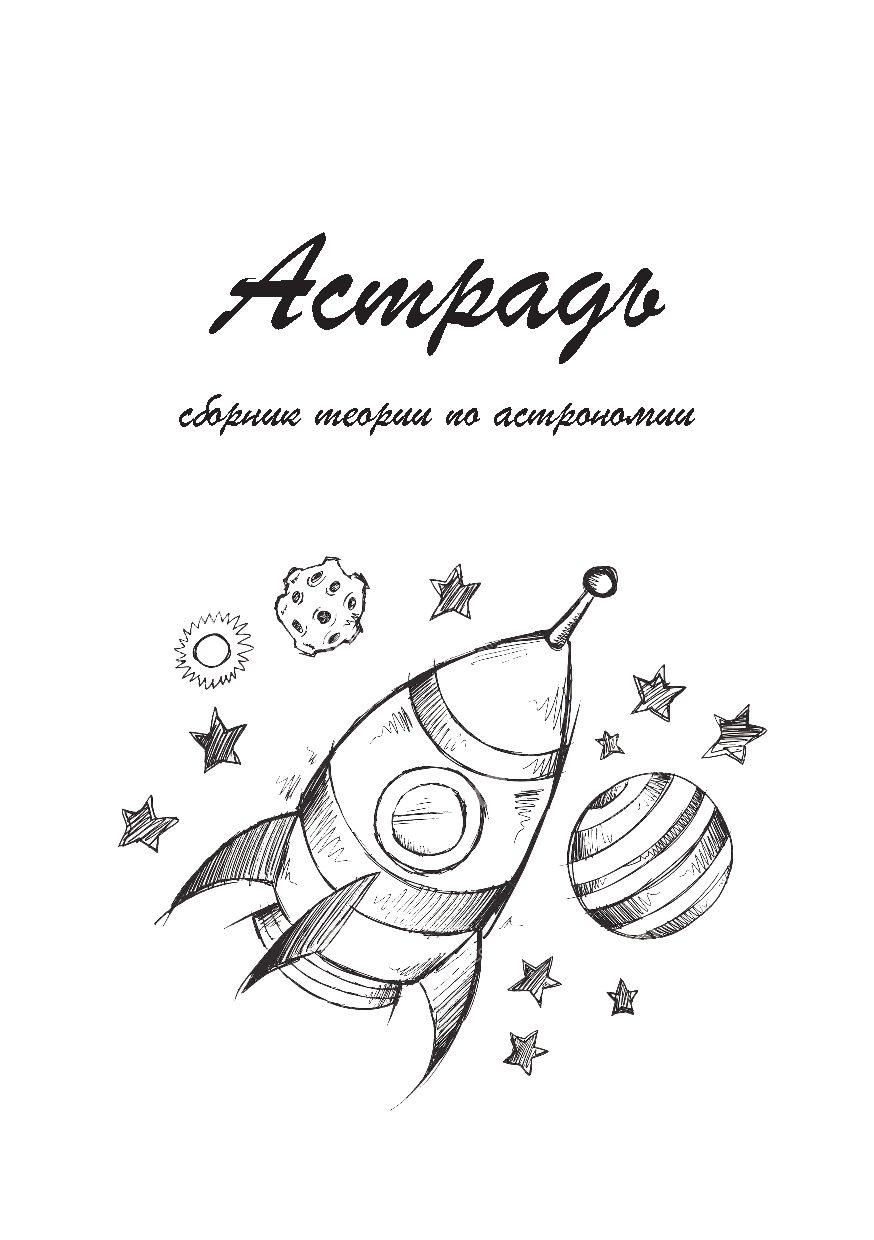
\includegraphics[width=0.95\tw]{sys/cover.pdf}\\[1pc]
{\scshape Beograd, Srbija \\ \year}	
\end{center}

	\newpage
\setcounter{page}{2}
\thispagestyle{empty}
	\noindent ББК 22.6\\
%	\hspace*{1.8pc} 
	A 91\\
	УДК 52\\[1pc]

{\small {\itshape Рецензент:}\\ учитель астрономии М.\,В.~Кузнецов (МОУ Гимназия №1~~г.\,о.~Жуковский)}\\[1pc]

{\small {\itshape Редакторы:}\\ 
выпускник Московского государственного университета А.\,В.~Афанасьев,\\
магистр политехнического института Гренобля, бакалавр Московского физико-тех\-ни\-чес\-кого института В.\,А.~Сушко\\[1pc]}


{%\hspace{1pc} 
{\bfseries А.\,С.~Шепелев, Д.\,А.~Долгов, С.\,Д.~Молчанов, С.\,Б.~Борисов}\\ Астрадь~--- краткий сборник теории по астрономии. 2020.~---~64~с: 2-е изд. ISBN 978-5-9909877-1-5\\[2pc]

{\small Астрадь является учебным пособием по астрономии, рекомендованным для школьников 7\,--\,11 класса. Сборник составлен неоднократными призерами международных олимпиад по астрономии, членами астрономического кружка им.~Е.\,П.~Левитана г.\,о.~Жуковский. 

Здесь читатель сможет найти необходимый минимум теории для участия в различных олимпиадах школьников по астрономии. Также Астрадь можно использовать и для освоения школьной программы, потому что наряду со сложными темами освещены и самые базовые вопросы астрономии.}\\[1pc]

{\small{\itshape Вёрстка:} А.\,С.~Шепелев}\\ \vfill


\noindent\begin{minipage}[t]{0.4\tw}
	{\bfseries ISBN 978-5-9909877-1-5}
\end{minipage}
\hfill
\begin{minipage}[t]{0.57\tw}
	\small
	\copyright\,А.\,С.~Шепелев, Д.\,А.~Долгов,\\
	 \hspace*{8pt} С.\,Д.~Молчанов, С.\,Б.~Борисов, 2018\\[3pt]
	\copyright\,Астрономический кружок\\ \hspace*{8pt} им.~Е.\,П.~Левитана г.\,о.~Жуковский, 2018
\end{minipage}
\newpage
	\setcounter{tocdepth}{2}
	{
		\small
		\renewcommand{\baselinestretch}{ 0.9 }
		\tableofcontents
		\label{toc}
		\renewcommand {\baselinestretch}{ 1.02 }
	}
	\newpage
	\section{Геометрическая астрономия}
\label{sec:geometrical-astronomy}

\subsection{Расстояние и размеры}
В астрономии наравне с единицами Международной системы единиц, СИ, используются внесистемные единицы измерения длины.
Одна из них, \term{Астрономическая единица}~--- единица измерения расстояния в астрономии, 
\begin{equation}
	1~\au = 149\:597\:870\:700~\text{м} \simeq 1.5 \times 10^{11}~\text{м},
\end{equation}
величина которой близка к длине большой полуось орбиты Земли. Точное значение было привязано к метру на Генеральной Асамблеи Международного Астрономического Союза в 2012 году~\cite{au}.

Астрономическая единица используется для описания расстояний между объектами Солнечной системы и экзопланетных систем. Расстояния между звездами и размеры более крупных формирований имеют существенно большую величину, чем астрономическая единица, поэтому здесь она не используется.

\begin{wrapfigure}[7]{r}{0.45\tw}
	\centering
	\vspace{-1.3pc}
	\begin{tikzpicture}	    
	    \tkzDefPoint(0,0){Sun}
	    \tkzDefPoint(3,0){Star}
	    \tkzDefPoint(0,1){E}

	    \tkzLabelPoint[above](E){Земля}
	    \tkzLabelPoint[below](Sun){Солнце}
	    \tkzLabelPoint[below](Star){Звезда}
	    
	    \tkzDrawCircle[dashed, black, line width=.5pt](Sun,E)
	    \tkzDrawPolygon[thick](Sun,Star,E)
	    \tkzMarkRightAngle[size=0.2](Star,Sun,E)
	    \tkzMarkAngle(E,Star,Sun)
	    \tkzLabelAngle[font=\footnotesize, pos=1.2](E,Star,Sun){$p$}   
	    
	    \earth(E)
	    \sun(Sun)
	    \pointStar(Star)
	    
	    \tkzLabelSegment[below](Sun,Star){$r$}
	    \tkzLabelSegment[left=-2pt](Sun,E){1\,\text{а.\!\:е.}}
	\end{tikzpicture}
	\caption{Схема годичного параллакса}
\end{wrapfigure}
Первым методом определения расстояния до звёзд был \imp{годичный параллакс}, основанный на видимом движении звезды в результате орбитального движения Земли. \term{Годичный параллакс} $p$ объекта~--- это угол, под которым отрезок длины 1~\au из окрестностей данного объекта, применяется к объектам вне
Солнечной системы.
\begin{equation}
	\tg p = \frac{1~\text{\au}}{r},
	\label{eq:parallax-sin}
\end{equation}
где $r$~--- расстояние до объекта. Учитывая малость угла $p$, можно считать $\tg p \simeq p$ в \eqref{eq:parallax-sin}, тогда
\begin{equation}
	p \simeq \frac{1~\text{\au}}{r}.
	\label{eq:parallax}
\end{equation}

С помощью параллакса вводится ещё одна внесистемная единица длина, используемая в астрономии,~--- \term{парсек}. Это такое расстояние~$r$, что, находясь на нём, произвольный объект имеет годичный параллакс~$p = 1''$. Напомним,
\begin{equation*}
	1~\text{рад} = \frac{180^\circ}{\pi} =  \frac{10800'}{\pi} = \frac{648000''}{\pi} \simeq 206265'',
\end{equation*}
следовательно, 
\begin{equation}
    1~\text{пк} = \frac{648000}{\pi}~\text{\au} \simeq 3.085677581 \cdot 10^{16}~\text{м} \simeq 206265~\au
\end{equation}
В силу определение парсека, справедливо соотношение
\begin{equation}
	r~\lbrack \text{пк} \rbrack 
	   = \frac{1~\lbrack \au \rbrack}{\pi~\lbrack '' \rbrack}.
\end{equation}


Достаточно часть в астрономии имеет значение \term{угловой размер объекта}~--- угол, под которым видно объект. Для несимметричных объектов понимается некая средняя величина, для объектов с осевой симметрией, например галактик, указывается два размера вдоль каждой из осей. Для сферически симметричных объектов с радиусом $R$, угловой размер (диаметр) при наблюдении с расстояния $r$, \lookPicRef{pic:angilar-size}, определяется как\\
\begin{wrapfigure}[9]{r}{0.45\tw}
		\centering
		\vspace{-2pc}
		\begin{tikzpicture}
            \tkzDefPoint(0,0){C}
            \tkzDefPoint(4,0){O}
            \tkzDefPointBy[homothety=center C ratio .25](O) \tkzGetPoint{U}
            
            \tkzDrawCircle[color=black, fill=gray!40, thick](C,U)
            \tkzDefLine[tangent from = O](C,U) \tkzGetPoints{I1}{I2}
            \tkzDrawSegments(C,I1 C,I2 C,O)
            \tkzDrawSegments[thick](O,I2 O,I1)
            \tkzMarkRightAngles[size=0.2](O,I1,C C,I2,O)
            \tkzMarkAngle[size=1.2](I2,O,C)
            \tkzMarkAngle[size=1.1](C,O,I1)
            
            \tkzLabelSegment[left](C,I1){$R$}
            \tkzLabelSegment[left](C,I2){$R$}
            \tkzLabelSegment[above](C,O){$r$}
            
            \DeclareCollectionInstance{angular-size-xfrac}{xfrac}{mathdefault}{math}{
                denominator-bot-sep = -1pt,
                slash-symbol = \scalebox{0.9}{/},
                numerator-bot-sep = 3pt,
                scaling= true,
                slash-right-mkern= -2 mu,
                slash-left-mkern= -1.5 mu
            }
            \UseCollection{xfrac}{angular-size-xfrac}
            
            \tkzLabelAngle[pos=1.5](I2,O,C){$\sfrac{\rho}{2}$}
            \tkzLabelAngle[pos=1.5](C,O,I1){$\sfrac{\rho}{2}$}
            
            \tkzDrawPoints(C, O, I1, I2)
        \end{tikzpicture}
    	\caption{Угловой размер}
		\label{pic:angilar-size}
	\end{wrapfigure}
\vspace{-2pc}
\begin{equation}
	\rho = 2 \arcsin \frac{R}{r}.
\end{equation}
В случае, когда $r\gg R$, можно считать, что $\sin \rho \simeq \rho$, тогда
\begin{equation}
	\rho \simeq \frac{2 R}{r}.
\end{equation}

\begin{wrapfigure}[6]{r}{0.45\tw}
	\centering
	\vspace{-1.5pc}
	\begin{tikzpicture}
            \tkzDefPoint(0,0){O}
            \tkzDefPoint(4,0){S}
            \tkzDefPointBy[homothety=center O ratio .25](S) \tkzGetPoint{X}
            \tkzDefPointBy[rotation=center O angle -90](X) \tkzGetPoint{C}
            
            \tkzDrawCircle[color=black, fill=gray!40, thick](C,O)

            \tkzDrawSegments[thick](O,S C,S)
            \tkzDrawSegments(C,O)
            \tkzMarkRightAngles[size=0.2](C,O,S)
            \tkzMarkAngle(O,S,C)

            
            \tkzLabelSegment[below](C,S){$r$}
            \tkzLabelSegment[left=-2pt](C,O){$R_\oplus$}
            \tkzLabelAngle[pos=1.3, font=\footnotesize](O,S,C){$p$}
            
            \tkzDrawPoints(C, O, S)
        \end{tikzpicture}
		\caption{Горизонтальный параллакс}
		\label{pic:horizontal-parallax}
\end{wrapfigure}
Для определения расстояния до объектов Солнечной системы также используется метод параллакса. Измеряемая величина $p$ называется \term{горизонтальным параллаксом}, \lookPicRef{pic:horizontal-parallax},~--- это угловой радиус Земли при наблюдении из окрестностей объекта:
\begin{equation}
	\sin p =\frac{R_\oplus}{r}.
\end{equation}
Так, средний горизонтальный параллакс Луны $p_{\rightmoon}$ составляет около $1^\circ$, а Солнца~--- $p_\odot \approx 9''$.

\subsection{Параллактический эллипс}
Движение Земли по орбите вокруг Солнца сопровождается изменением видимого положения объектов вне Солнечной системы. В приближении круговой орбиты движение Земли циклично, а значит, траектории объектов относительно геоцентрической системы координат также цикличны. Чтобы установить, что из себя представляют данные траектории необходимо спроецировать годичное движение Земли на плоскость, перпендикулярную лучу зрения на объект.

Проекция окружности всегда эллипс, кроме вырожденного случая~--- отрезка, когда угол проекции составляет $90^\circ$. Так как проецирование с углом $\eta$ между плоскостями~--- тоже самое, что сжатие с коэффициентом $1/\cos\eta$.

\begin{wrapfigure}{r}{0.6\tw}
	\centering
	\begin{tikzpicture}
		\footnotesize
		
		%		\clip (-5, -3.5) rectangle (3.5, 3.5);
		
		%		\foreach \x in {-5, -4.9,...,3} {
		%		\draw [line width=.1pt] (\x, -3) -- (\x, 3);
		%		};
		%
		%		\foreach \x in {-5, -4,...,3} {
		%		\draw [line width=.4pt] (\x , -3) -- (\x , 3);
		%		};
		%
		%		\foreach \y in {-3, -2.9,...,3} {
		%		\draw [line width=.1pt] (-5, \y) -- (3, \y);
		%		};
		%
		%		\foreach \y in {-3, -2,...,3} {
		%		\draw [line width=.4pt] (-5, \y) -- (3, \y);
		%		};
		
		\coordinate (O) at (0, 0) {};
		\coordinate (A1) at (-0.57, 0.98) {};
		\coordinate (A2) at (0.57, -0.98) {};
		\coordinate (B1) at (-3, 0) {};
		\coordinate (B2) at (3, 0) {};
		\coordinate (C1) at (1.5, 2.6) {};
		\coordinate (C2) at (-1.5, -2.6) {};
		\coordinate (D1) at (.75, 1.3) {};
		\coordinate (D2) at (-.75, -1.3) {};
		\coordinate (S) at (-3.5, 2) {};
		
		\draw [decoration={zigzag, segment length=1.1mm, amplitude=0.3mm}, decorate] (-2.8, 1.6) arc(-30:-10:0.81);
		\draw [double, line cap=butt](-.3, 0) arc(180:150:.3);
		\draw [double, line cap=butt](2.7, 0) arc(180:150:.3);
		\draw [decoration={snake, segment length=1mm, amplitude=0.3mm}, decorate](0.3, 0) arc(0:60:.3);
		\draw (.65, 1.127) -- (0.823, 1.027) -- (0.923, 1.2);
		\draw (.12, -0.2) -- (.35, -.2) -- (.23, 0);
		\draw (-2.14, 1.0) .. controls (-2.04, 1.07) .. (-2.1, 1.2);
		
		\draw (O) ellipse(3 and 1);
		%		\draw (O) [rotate=60, dashes] ellipse(3 and 1);
		
		\draw (A1) .. controls (-.2, 1.54) and (.5, 1.55) .. (D1);
		\draw (A2) .. controls (1.17, -.1) and (1.25, .9) .. (D1);
		\draw (A2) .. controls (.2, -1.54) and (-.5, -1.55) .. (D2);
		\draw (A1) .. controls (-1.17, .1) and (-1.25, -.9) .. (D2);
		
		\draw [dashes] (D1) -- (D2);
		\draw [dashes] (B1) -- (B2);
		\draw [dashes] (D1) -- (3, 0);
		
		\draw (A1) -- (A2);
		\draw (O) -- (S);
		\draw (D1) -- (S);
		\draw (A2) -- (S);
		
		\pointStar (S);
		
		\point (A1);
		\point (A2);
		\point (B1);
		\point (B2);
		\point (O);
		\point (D1);
		\point (D2);
		
		\draw (-2.75, 1.82) node[anchor=north west] {$\pi_\beta$};
		\draw (-1.85, 1.15) node[anchor=north] {$\pi_\alpha$};
		\draw (-.4, .15) node[anchor=east] {$\beta$};
		\draw (.25, .05) node[anchor=south west] {$\eta$};
		
	\end{tikzpicture}
	\caption{Схема построения параллактического эллипса}
\end{wrapfigure}
Траектория Земли для наблюдателя, находящегося в окрестности объекта,~--- эллипс. Тогда понятно, что траектория объекта для наблюдателя на Земле также является эллипсом. Причем большая полуось этого эллипса равна параллаксу объекта $\pi = a_\oplus / r \equiv \pi_\lambda$, где $r$~--- гелиоцентрическое расстояние до объекта, а малая полуось
\begin{equation*}
	\pi_\beta = \frac{a_\oplus \cos \eta}{r}.
\end{equation*}

Траектория (эллипс) видимого годичного движения объектов называется \term{параллактическим эллипсом}, эксцентриситет которого
\begin{equation*}
	e
	= \sqrt{1 - \left(\frac{\pi_\beta}{\pi_\lambda} \right)^2}
	= \sqrt{1 - \left( \frac{r \cdot a_\oplus \cos \eta}{a_\oplus \cdot r}\right)^2}
	= \sqrt{1 - \cos^2 \eta} = \sin \eta = \cos \beta,
\end{equation*}
где $\beta$~--- эклиптическая широта объекта.


\subsection{Кеплеровы элементы орбиты}
\begin{wrapfigure}[11]{r}{0.45\tw}
	\centering
	\vspace{-0.7pc}
	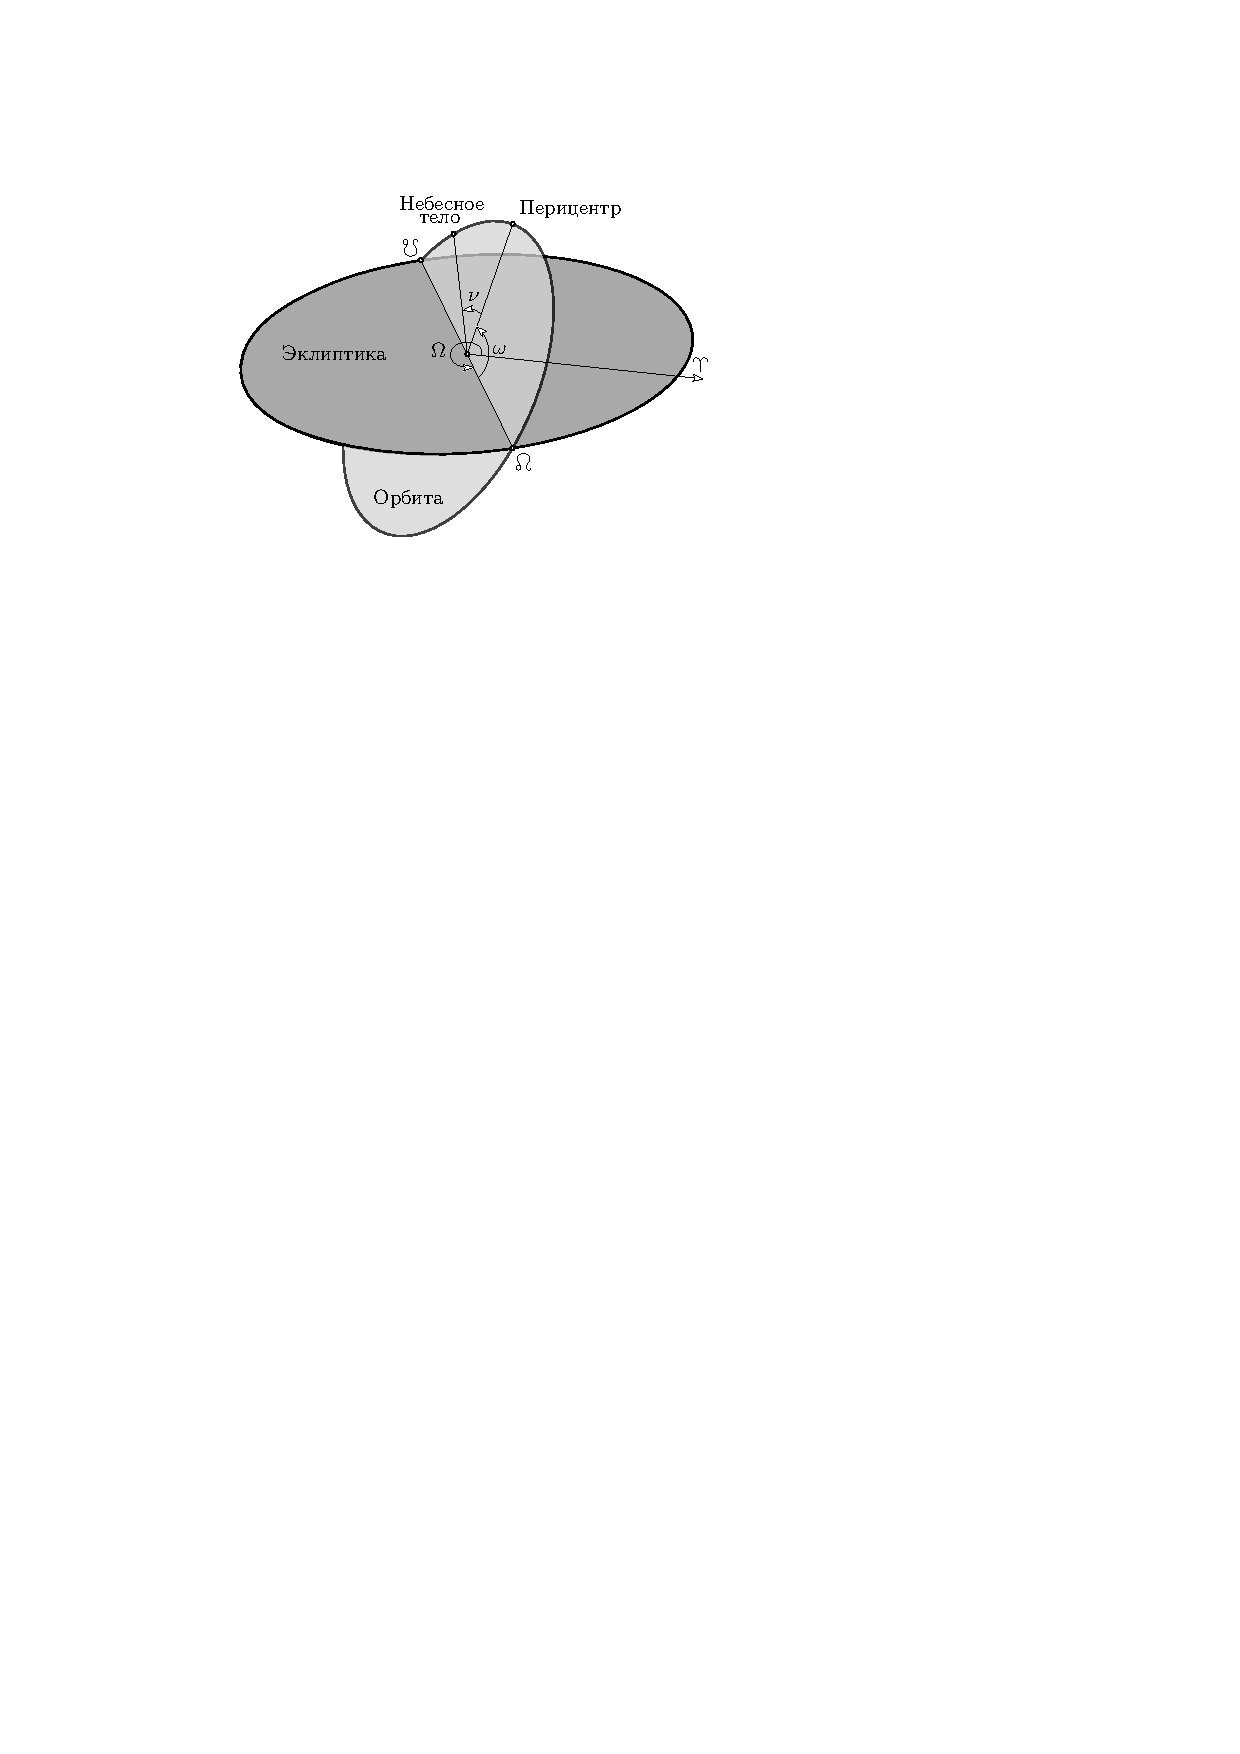
\includegraphics[width=.45\tw]{orbit-elem}
	\captionof{figure}{Кеплеровы элементы орбиты}
	\label{fig:orb-elem}
\end{wrapfigure}
\term{Кеплеровы элементы} используют для описания положения в пространстве тел, находящихся на орбите вокруг заданного гравитирующего центра. Это шесть параметров: первые два из них определяют геометрию орбиты тела~--- это \imp{большая полуось} ($a$) и \imp{эксцентриситет} ($e$). Следующие три описывают положение орбиты в пространстве: \imp{наклонение} ($i$), \imp{аргумент перицентра} ($\omega$) и \imp{долгота восходящего узла} ($\Omega$). Последний~--- \imp{истинная аномалия} ($\nu$), задает положение тела на орбите.

Для использования кеплеровых элементов для описания положения тел первоначально необходимо задать систему отсчета~--- выбрать базовую плоскость, проходящую через гравитирующий центр и луч в этой плоскости, исходящий из него. Для описания положения тел Солнечной системы за базовую плоскость принимают плоскость эклиптики, а за луч~--- направление на точку весеннего равноденствия, при описании положения тел в околопланетном пространстве~--- плоскость экватора и луч, образованный пересечение экватора и нулевого меридиана.

\term{Истинная аномалия} тела, движущегося по орбите~--- угол в плоскости орбиты с вершиной в фокусе этой орбиты между направлениями на перицентр орбиты и на тело. Возрастает в ходе орбитального движения, изменяется в промежутке $[0^\circ, 360^\circ)$.

\term{Аргумент перицентра}~--- угол между направлениями на восходящий узел орбиты и на перицентр при наблюдении из притягивающего центра (фокуса орбиты). Откладывается в сторону орбитального движения, может иметь значению в промежутке $[0^\circ, 360^\circ)$.

\term{Наклонение}~--- это угол между плоскостью орбиты небесного тела и плоскостью эклиптики. Принимает значения от $0^\circ$ до $90^\circ$.

\term{Долгота восходящего узла}~--- угол в базовой плоскости между базовым направлением и направлением восходящий узел орбиты. Отсчитывается против часов стрелки при наблюдении из северного полупространства, лежит в промежутке $[0^\circ, 360^\circ)$.

\term{Узлы орбиты}~--- точки пересечения орбиты и базовой плоскости. \imp{Восходящий узел}~--- точка, в которой тело пересекает базовую плоскость при движении в северноим направлении, а \imp{нисходящий}~--- в южном.

Кеплеровы элементы являются \imp{углами Эйлера}, описывающими поворот абсолютно твердого тела в трёхмерном евклидовом пространстве. Введём прямоугольную декартову систему координат, связанную с орбитой тела: фокус~--- начало координат, направление на перицентр~--- ось~$x$, ось~$z$~--- нормаль к плоскости орбиты в северном полупространстве. Ось~$y$~--- луч в плоскости орбиты такой, чтобы направляющие вектора $\vec e_x$, $\vec e_y$ и $\vec e_z$ образовывали правую тройку. 

Найдём правила перехода из описанной системы координат в прямоугольную декартову систему координат, связанную с базовой плоскостью и лучом. Положение тела в орбитальной системе координат можно определить вектором $\vec r = (r \cos \nu, r \sin \nu, 0)$. Перейдем в систему координат, повернутую на угол $-\omega$ вокруг оси~$z$:
\begin{multline*}
    \vec r' = Z'_\omega\vec r 
    = \begin{pmatrix}
        \cos \omega & - \sin \omega & 0\\
        \sin \omega & \cos \omega & 0\\
        0 & 0 & 1
    \end{pmatrix} \begin{pmatrix}
        r \cos \nu\\
        r \sin \nu\\
        0
    \end{pmatrix} = \\
    = \begin{pmatrix}
        r \cos \nu \cos \omega - r \sin \nu \sin \omega\\
        r \cos \nu \sin \omega + r \sin \nu \cos \omega\\
        0
    \end{pmatrix} 
    =\begin{pmatrix}
        r \cos (\nu + \omega)\\
        r \sin (\nu + \omega)\\
        0
    \end{pmatrix}.
\end{multline*}
Ось~$x$ текущей системы координат совпадает с направлением на восходящий узел орбиты. Перейдем в систему координат, повернутую на угол $-i$ вокруг оси~$x$:
\begin{equation*}
    \vec r'' = X'_i\vec r' 
%    = X_{-i}Z_{-\omega}\vec r 
    = \begin{pmatrix}
        1 & 0 & 0\\
        0 & \cos i & - \sin i\\
        0 & \sin i & \cos i
    \end{pmatrix}\begin{pmatrix}
        r \cos (\nu + \omega)\\
        r \sin (\nu + \omega)\\
        0
    \end{pmatrix} 
    = \begin{pmatrix}
        r \cos (\nu + \omega)\\
        r \sin (\nu + \omega) \cos i\\
        r \sin (\nu + \omega) \sin i
    \end{pmatrix}.
\end{equation*}
Теперь ось~$z$ является нормалью к базовой плоскости. Повернём оси координат на угол $-\Omega$ вокруг оси $z$:
\begin{multline*}
    \vec r''' = Z'_\Omega\vec r''
%    = X_{-i}Z_{-\omega}\vec r 
    = \begin{pmatrix}
        \cos \Omega & - \sin \Omega & 0\\
        \sin \Omega & \cos \Omega & 0\\
        0 & 0 & 1
    \end{pmatrix}\begin{pmatrix}
        r \cos (\nu + \omega)\\
        r \sin (\nu + \omega) \cos i\\
        r \sin (\nu + \omega) \sin i
    \end{pmatrix} = \\
    = \begin{pmatrix}
        r \cos (\nu + \omega) \cos \Omega - r \sin (\nu + \omega) \cos i \sin \Omega\\
        r \cos (\nu + \omega) \sin \Omega + r \sin (\nu + \omega) \cos i \cos \Omega\\
        r \sin (\nu + \omega) \sin i
    \end{pmatrix}.
\end{multline*}

Отсюда следует, что координаты тела, находящегося на расстоянии~$r$ от фокуса, в базовой системе координат задаются соотношением
\begin{equation*}
    \vec r_0 =
%   r K \vec e_x \equiv
    r Z'_\Omega X'_i Z'_{\omega + \nu} \vec e_x =
    r \begin{pmatrix}
        \cos (\nu + \omega) \cos \Omega - \sin (\nu + \omega) \cos i \sin \Omega\\
        \cos (\nu + \omega) \sin \Omega + \sin (\nu + \omega) \cos i \cos \Omega\\
        \sin (\nu + \omega) \sin i
    \end{pmatrix}.
\end{equation*}









\nopagebreak
\subsection{Затмения}
Диаметр тени спутника при полном центральном затмении (когда центры трёх тел лежат на одной прямой) с большой точностью равен
\begin{equation}
	d_\text{тени} = 2 \cdot \frac{R_{\moon}(a_\oplus - R_\oplus) - R_\odot \left( a_{\moon} - R_\oplus \right)}{a_\oplus - a_{\moon}}.
\end{equation}

\begin{figure}[h!]
    \centering
    \begin{tikzpicture}
        \tkzDefPoint(0, 0){X}
        \tkzDefPoint(-3.5,0){C1}
        \tkzDefShiftPoint[C1](0.5,0){R1}
        
        \def\k{2.5}
        \tkzDefPointBy[homothety=center X  ratio \k](C1) \tkzGetPoint{C2}
        \tkzDefPointBy[homothety=center X  ratio \k](R1) \tkzGetPoint{R2}
        
        \tkzDefLine[tangent from = X](C1,R1) \tkzGetPoints{A1}{B1}
        \tkzDefLine[tangent from = X](C2,R2) \tkzGetPoints{A2}{B2}
        
        \tkzDrawPolygon[fill=gray!40,draw=none](X,A1,B1)
        
        \tkzDrawCircles[fill=white, thick, draw=black](C1,R1 C2,R2)
        \tkzDrawSegments(X,A2 X,B2 X,C2 C2,A2 C2,B2 C1,A1 C1,B1)
        
        \tkzLabelSegments[left=-1pt](C2,B2 C2,A2){$R$}
        \tkzLabelSegments[left=-2pt](C1,B1 C1,A1){$r$}
        \tkzLabelSegment[above=-1.5pt](C1,C2){$d$}
        \tkzLabelSegment[above=-1.5pt](C1,X){$x$}
        
        \tkzMarkRightAngles[size=0.15](C2,A2,X X,B2,C2 C1,A1,X X,B1,C1)
        \tkzDrawPoints(C1, C2, A1, A2, B1, B2, X)
    \end{tikzpicture}
    \caption{\change{Схема построение тени}}
    \label{pic:shadow-length}
\end{figure}

\begin{figure}[h!]
    \centering
    \begin{tikzpicture}
        \tkzDefPoint(0, 0){X}
        \tkzDefPoint(-5,0){C1}
        \tkzDefShiftPoint[C1](0.7,0){R1}
        \tkzDefPoint(-0.5,0){C3}
        \tkzDefShiftPoint[C3](-0.9,0){R3}
        
        \def\k{1.7}
        \tkzDefPointBy[homothety=center X  ratio \k](C1) \tkzGetPoint{C2}
        \tkzDefPointBy[homothety=center X  ratio \k](R1) \tkzGetPoint{R2}
        
        \tkzDefLine[tangent from = X](C1,R1) \tkzGetPoints{A1}{B1}
        \tkzDefLine[tangent from = X](C2,R2) \tkzGetPoints{A2}{B2}
        
        \tkzInterLC(X,B1)(C3,R3)  \tkzGetPoints{x}{H1}
        \tkzInterLC(X,A1)(C3,R3)  \tkzGetPoints{H2}{x}
        
        \tkzDrawPolygon[fill=gray!40,draw=none](X,A1,B1)
        
        
        \tkzDrawCircles[fill=white, thick, draw=black](C1,R1 C2,R2 C3,R3)
        \tkzDrawSegments(H2,A2 H1,B2 R3,C2 C2,A2 C2,B2 C1,A1 C1,B1)
        \tkzDrawSegments[dashed](H2,X H1,X R3,X)
        
        \begin{scope}[
            dim style/.style={black, latex-latex, opacity=1},
            dim fence style/.style={black, opacity=1}
        ]
            \tkzDrawSegment[opacity=0, dim={$R$, -1cm, above=2pt}](C3,R3)
            \tkzDrawSegment[opacity=0, dim={$d_2$, -1.4cm, above=2pt}](C3,C1)
            \tkzDrawSegment[opacity=0, dim={$d_1$, -1.8cm, above=2pt}](C3,C2)
            \tkzDrawSegment[opacity=0, dim={$h$, 1cm, below=2pt}](X,R3)
            \tkzDrawSegment[opacity=0, dim={$x$, 1.4cm, above=2pt}](X,C1)
        \end{scope}
        
        \tkzLabelSegments[right=-1pt](C2,B2 C2,A2){$R_0$}
        \tkzLabelSegments[right=-2pt](C1,B1 C1,A1){$r$}
        \tkzLabelSegments[left=-2pt](R3,H1 R3,H2){$s$}
        
        \tkzMarkRightAngles[size=0.15](C2,A2,X X,B2,C2 C1,A1,X X,B1,C1)
        \tkzDrawPoints(C1, C2, A1, A2, B1, B2, X, C3, R3, H1, H2)
    \end{tikzpicture}
    \caption{\change{К вычислению диаметра пятна}}
    \label{pic:shadow-size-on-surface}    
\end{figure}


Среднее значение  этой величины около 200~км, максимальное~--- около 215~км. При нецентральном затмении максимальный диаметр тени Луны на поверхности Земли может достигать 270~км. Это даёт оценку на продолжительность, равную 7.5 минутам. Большинство полных затмений длятся 2\,--\,4~минуты.

\begin{figure}[h!]
	\centering
	\vspace{-.5pc}
	\begin{tikzpicture}[xscale=1.2]
            
        \tkzInit[
            xmax=1,
            xmin=-7,
            ymin=-1.2,
            ymax=1.2
        ]
        \tkzClip    
            
        \def\e{0}
        \def\m{-1.3}
        \def\s{-6}
        
        \def\earthR{0.7}
        \def\moonR{0.18}
        \def\sunR{1}
        
        \tkzDefPoint(\e,0){E}
        \tkzDefPoint(\m,0){M}
        \tkzDefPoint(\s,0){S}
        
        
        
        \tkzDefShiftPoint[S](0,\sunR){S'}
        \tkzDefShiftPoint[M](0,\moonR){M'}
        \tkzDefShiftPoint[E](0,\earthR){E'}
        
        \def\shadeCornerCoef{\sunR / (\sunR - \moonR)}
        \tkzDefPointBy[homothety=center S ratio \shadeCornerCoef](M)
        \tkzGetPoint{SC}
        
        \def\halfShadowCornerCoef{\sunR / (\sunR + \moonR)}
        \tkzDefPointBy[homothety=center S ratio \halfShadowCornerCoef](M)
        \tkzGetPoint{HSC}
        
        \tkzDefLine[tangent from = SC](S,S')  \tkzGetPoints{S1}{S2}
        \tkzDefLine[tangent from = SC](M,M')  \tkzGetPoints{M1}{M2}
        \tkzDefLine[tangent from = HSC](S,S')  \tkzGetPoints{HS1}{HS2}
        \tkzDefLine[tangent from = HSC](M,M')  \tkzGetPoints{HM1}{HM2}
        
        \tkzInterLC(SC,S1)(E,E') \tkzGetSecondPoint{E1}
        \tkzInterLC(SC,S2)(E,E') \tkzGetFirstPoint{E2}
        
        \tkzGetVectxy(HSC,M){hs}
        \def\halfShadowCoef{(\e - \m + \hsx) / \hsx }
        \tkzDefPointBy[homothety=center HSC ratio \halfShadowCoef](HM1)
        \tkzGetPoint{HE1}
        \tkzDefPointBy[homothety=center HSC ratio \halfShadowCoef](HM2)
        \tkzGetPoint{HE2}
        
        
        \tkzDrawSector[fill=gray!30,gray!30](HSC,HE2)(HE1)
        \tkzDrawSector[fill=gray!70](SC,M2)(M1)
        \tkzDrawSector[fill=white](HSC,HM2)(HM1)
        
        \tkzDrawCircles[dashed, line width=.4pt](S,E E,M) 

        \tkzDrawCircles[black, line width=.4pt, fill=white](S,S' M,M')
        \tkzDrawSegments(SC,S1 SC,S2 HS1,HE1 HS2,HE2)
%        \tkzDrawSegments(S,S1 S,S2 S,HS1 S,HS2 M,M1 M,M2 M,HM1 M,HM2)
%        \tkzDrawPoints(S1, S2, SC, HS1, HS2, M1, M2, HM1, HM2)
        
        \tkzDrawCircles[black, line width=.4pt, fill=white, fill opacity=1](E,E')
%        \tkzDrawPoints(E1, E2)
        
        \tkzLabelPoint[inner sep=5mm](S){\tikz{\sun(S)}}
        \tkzLabelPoint(E){\tikz{\earth(E)}}
        \tkzLabelPoint(M){$\rightmoon$}
    \end{tikzpicture}
	\caption{Полное солнечное затмение со стороны северного полюса эклиптики}
	\label{fig:eclipses-full-solar-eslipse}
\end{figure}
При \term[кольцеобразное солнечное затмение]{кольцеобразном солнечном затмении} Луна так расположена относительно Земли, что конус её тени не достаёт до поверхности планеты, и вокруг Луны можно наблюдать яркое кольцо незакрытой части солнечного диска.

\begin{figure}[h!]
	\centering
	\begin{tikzpicture}[xscale=1.2]
	
	    \tkzInit[
            xmax=1,
            xmin=-7,
            ymin=-1.2,
            ymax=1.2
        ]
        \tkzClip
            
        \def\e{0}
        \def\m{-1.8}
        \def\s{-6}
        
        \def\earthR{0.7}
        \def\moonR{0.18}
        \def\sunR{1}
        
        \tkzDefPoint(\e,0){E}
        \tkzDefPoint(\m,0){M}
        \tkzDefPoint(\s,0){S}
        
        
        \tkzDefShiftPoint[S](0,\sunR){S'}
        \tkzDefShiftPoint[M](0,\moonR){M'}
        \tkzDefShiftPoint[E](0,\earthR){E'}
        
        \def\shadeCornerCoef{\sunR / (\sunR - \moonR)}
        \tkzDefPointBy[homothety=center S ratio \shadeCornerCoef](M)
        \tkzGetPoint{SC}
        
        \def\halfShadowCornerCoef{\sunR / (\sunR + \moonR)}
        \tkzDefPointBy[homothety=center S ratio \halfShadowCornerCoef](M)
        \tkzGetPoint{HSC}
        
        \tkzDefLine[tangent from = SC](S,S')  \tkzGetPoints{S1}{S2}
        \tkzDefLine[tangent from = SC](M,M')  \tkzGetPoints{M1}{M2}
        \tkzDefLine[tangent from = HSC](S,S')  \tkzGetPoints{HS1}{HS2}
        \tkzDefLine[tangent from = HSC](M,M')  \tkzGetPoints{HM1}{HM2}
        
        \tkzInterLC(SC,S1)(E,E') \tkzGetSecondPoint{E1}
        \tkzInterLC(SC,S2)(E,E') \tkzGetFirstPoint{E2}
        
        \tkzGetVectxy(HSC,M){hs}
        \def\halfShadowCoef{(\e - \m + \hsx) / \hsx }
        \tkzDefPointBy[homothety=center HSC ratio \halfShadowCoef](HM1)
        \tkzGetPoint{HE1}
        \tkzDefPointBy[homothety=center HSC ratio \halfShadowCoef](HM2)
        \tkzGetPoint{HE2}
        
        \tkzDefPointBy[homothety=center SC ratio -1](M1) \tkzGetPoint{SC1}
        \tkzDefPointBy[homothety=center SC ratio -1](M2) \tkzGetPoint{SC2}
        
        \tkzDrawSector[fill=gray!30,gray!30](HSC,HE2)(HE1)
        \tkzDrawSector[fill=gray!70](SC,M2)(M1)
        \tkzDrawSector[fill=gray!50](SC,SC2)(SC1)
        \tkzDrawSector[fill=white](HSC,HM2)(HM1)

        \tkzDrawCircles[dashed, line width=.4pt](S,E E,M) 

        \tkzDrawCircles[black, line width=.4pt, fill=white](S,S' M,M')
        \tkzDrawSegments(SC,S1 SC,S2 HS1,HE1 HS2,HE2)
%        \tkzDrawSegments(S,S1 S,S2 S,HS1 S,HS2 M,M1 M,M2 M,HM1 M,HM2)
%        \tkzDrawPoints(S1, S2, SC, HS1, HS2, M1, M2, HM1, HM2)
        
        \tkzDrawCircles[black, line width=.4pt, fill=white, fill opacity=1](E,E')
%        \tkzDrawPoints(E1, E2)
        
        \tkzLabelPoint[inner sep=5mm](S){\tikz{\sun(S)}}
        \tkzLabelPoint(E){\tikz{\earth(E)}}
        \tkzLabelPoint(M){$\rightmoon$}
    \end{tikzpicture}
%	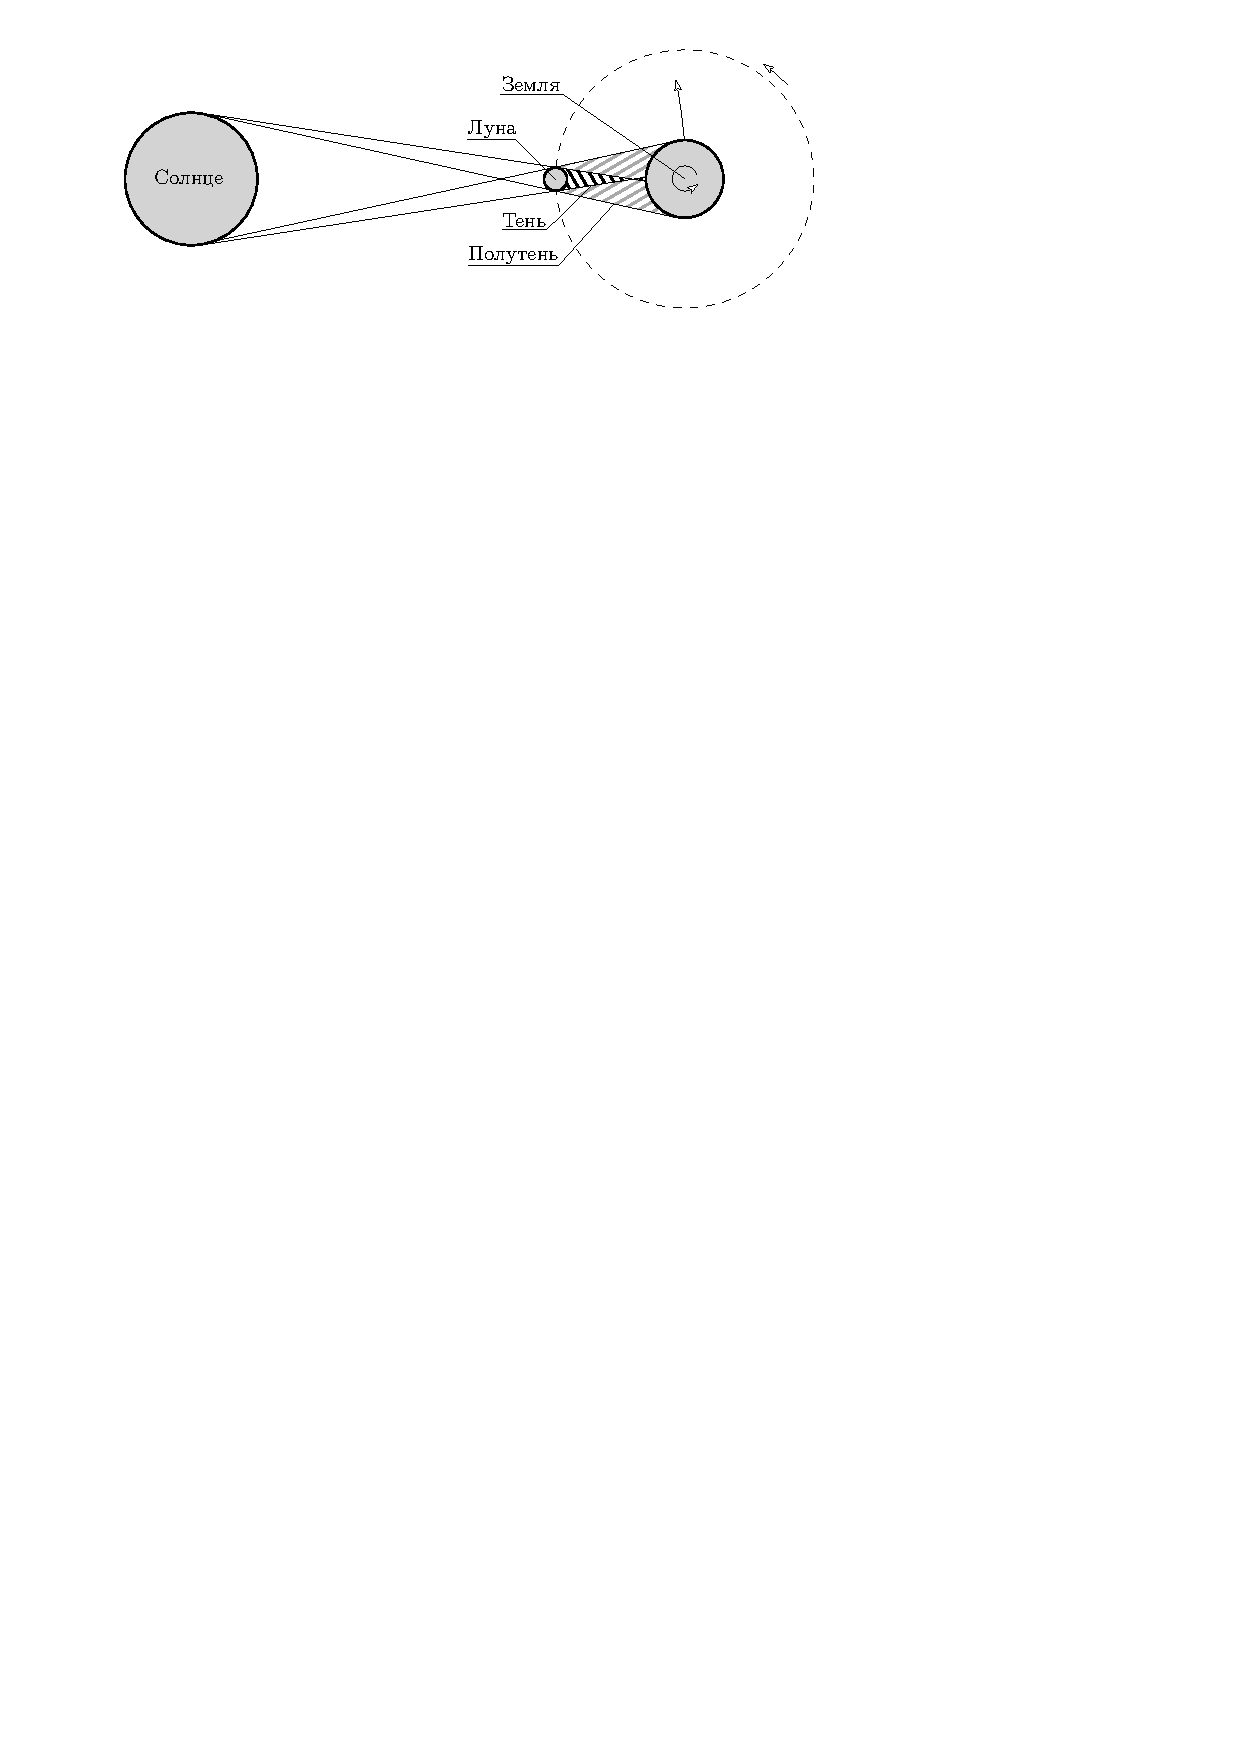
\includegraphics[width = 10cm]{partly-eclipse}
	\caption{Кольцеобразное солнечное затмение со стороны северного полюса эклиптики}
	\label{fig:eclipses-circle-solar-eslipse}
\end{figure}
При особом расположении Луны и Земли возможны \term{гибридные} затмения, когда в разных пунктах Земли наблюдаются либо \imp{кольцеобразное}, либо \imp{полное} затмение. Причиной такого явления является шарообразность Земли.

\vspace{-1pc}
\begin{figure}[h!]
	\centering
	\begin{tikzpicture}[xscale=1.2]
            
        \tkzInit[
            xmax=2.2,
            xmin=-7,
            ymin=-1.2,
            ymax=1.2
        ]
        \tkzClip
            
        \def\e{1.8}
        \def\m{0}
        \def\s{-6}
        
        \def\earthR{0.25}
        \def\moonR{0.7}
        \def\sunR{1}
        
        \tkzDefPoint(\e,0){E}
        \tkzDefPoint(\m,0){M}
        \tkzDefPoint(\s,0){S}
        
        
        \tkzDefShiftPoint[S](0,\sunR){S'}
        \tkzDefShiftPoint[M](0,\moonR){M'}
        \tkzDefShiftPoint[E](0,\earthR){E'}
        
        \def\shadeCornerCoef{\sunR / (\sunR - \moonR)}
        \tkzDefPointBy[homothety=center S ratio \shadeCornerCoef](M)
        \tkzGetPoint{SC}
        
        \def\halfShadowCornerCoef{\sunR / (\sunR + \moonR)}
        \tkzDefPointBy[homothety=center S ratio \halfShadowCornerCoef](M)
        \tkzGetPoint{HSC}
        
        \tkzDefLine[tangent from = SC](S,S')  \tkzGetPoints{S1}{S2}
        \tkzDefLine[tangent from = SC](M,M')  \tkzGetPoints{M1}{M2}
        \tkzDefLine[tangent from = HSC](S,S')  \tkzGetPoints{HS1}{HS2}
        \tkzDefLine[tangent from = HSC](M,M')  \tkzGetPoints{HM1}{HM2}
        
%        \tkzInterLC(SC,S1)(E,E') \tkzGetSecondPoint{E1}
%        \tkzInterLC(SC,S2)(E,E') \tkzGetFirstPoint{E2}
        
        \tkzGetVectxy(HSC,M){hs}
        \def\halfShadowCoef{1 + (\e - \m + \hsx) / \hsx }
        \tkzDefPointBy[homothety=center HSC ratio \halfShadowCoef](HM1)
        \tkzGetPoint{HE1}
        \tkzDefPointBy[homothety=center HSC ratio \halfShadowCoef](HM2)
        \tkzGetPoint{HE2}
        
        
        \tkzDrawSector[fill=gray!30,gray!30](HSC,HE2)(HE1)
        \tkzDrawSector[fill=gray!70](SC,M2)(M1)
        \tkzDrawSector[fill=white](HSC,HM2)(HM1)
        
        
        \tkzDrawCircles[dashed, line width=.4pt](S,M M,E)

        \tkzDrawCircles[black, line width=.4pt, fill=white](S,S' M,M')
        \tkzDrawSegments(SC,S1 SC,S2 HS1,HE1 HS2,HE2)
%        \tkzDrawSegments(S,S1 S,S2 S,HS1 S,HS2 M,M1 M,M2 M,HM1 M,HM2)
%        \tkzDrawPoints(S1, S2, SC, HS1, HS2, M1, M2, HM1, HM2)
        
        \tkzDrawCircles[black, line width=.4pt, fill=white, fill opacity=1](E,E')
%        \tkzDrawPoints(E1, E2)
        
        \tkzLabelPoint[inner sep=5mm](S){\tikz{\sun(S)}}
        \tkzLabelPoint(M){\tikz{\earth(E)}}
        \tkzLabelPoint(E){$\rightmoon$}
    \end{tikzpicture}
%	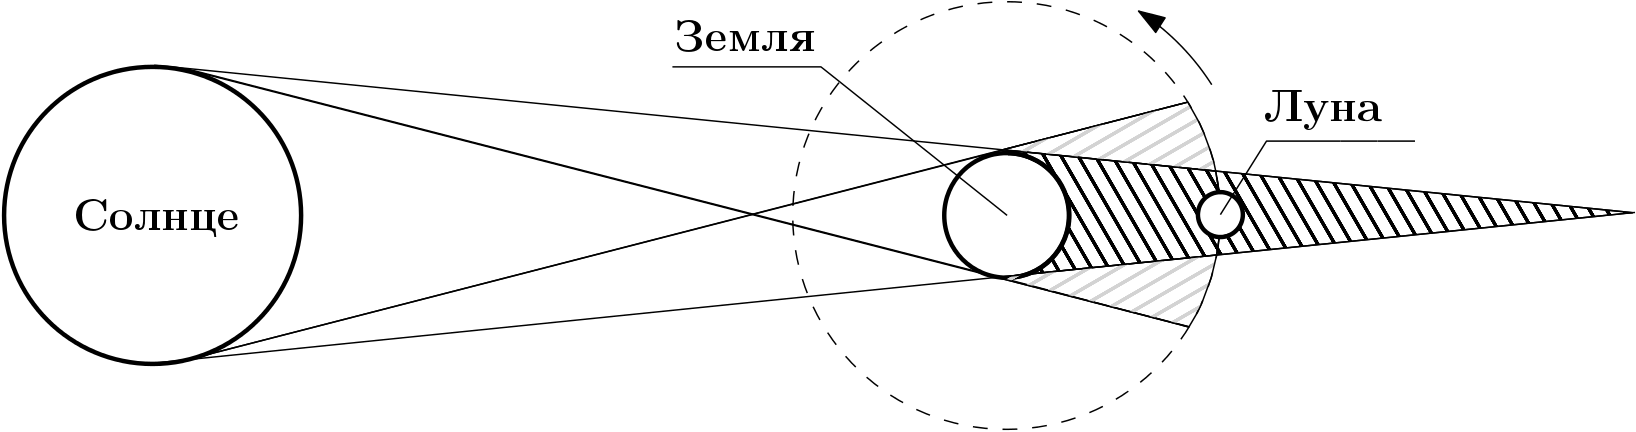
\includegraphics[width=10cm]{moon-eclipse}
	\caption{Схема лунного затмения со стороны северного полюса эклиптики}
	\label{fig:moon-eclipse-scheme}
\end{figure}
\term{Лунное затмение}, в отличие от солнечного, видно со всего ночного полушария Земли. Диаметр земной тени на расстоянии Луны превышает размер последней примерно в 2.5\,--\,3 раза. Бывают \term[частное затмение]{частные}, когда лишь часть Луны попадает в земную тень, \term[полное затмение]{полные}~--- Луна полностью погружается в тень Земли, и \term[полутеневое затмение]{полутеневые}~--- Луна проходит через полутень Земли, не затрагивая конус тени.

\term{Синодический месяц}~--- промежуток времени между одинаковыми фазами Луны, равен 29.53 суток.

\term{Драконический месяц}~--- промежуток времени между двумя последовательными прохождениями Луны через один и тот же узел орбиты,~--- 27.21 суток.

\term{Сарос}~--- промежуток  времени, по прошествии которого солнечные и лунные затмения повторяются в прежнем порядке. Происходит это из-за того, что каждый сарос Луна, орбита Луны и Солнце возвращаются в прежнее положение относительно далёких звёзд. Сарос длится ровно 242 драконических месяца, или 223 синодических месяца, или 18 лет 11 дней 8 часов.

\begin{wrapfigure}[8]{r}{.42\tw}
	\centering
	\vspace{-1pc}
	\includegraphics[width = 0.2\textwidth]{phases}
	\hfill
	\includegraphics[width = 0.2\textwidth]{phases-2}
	\caption{Частное и полное затмение}
	\label{fig:part-eclipses-scheme}
\end{wrapfigure}
Важной характеристикой любого затмения является его \term{фаза}~--- для \imp{частных} и \imp{кольцеобразных} затмений: отношение закрытой части $x$ диаметра\footnote{Здесь имеется в виду \imp{угловой} диаметр} затмеваемого тела, проходящего через центр затмевающего тела, ко всему диаметру затмеваемого тела $D$; для \imp{полного}: единица плюс отношение расстояния\footnote{Расстояние между окружностями $l_1$ и $l_2$~--- это $\min |L_1L_2|$ по всем $L_1 \in l_1$ и $L_2 \in l_2$.} между краями дисков затмеваемого и затмевающего тел к диаметру затмеваемого тела $D$.
\begin{equation}
	\Phi_{\text{част}} = \frac{x}{D} < 1, \quad \quad \quad \Phi_{\text{полн}} =  1 + \frac{\min\{d_1, d_2\}}{D} > 1.
\end{equation}
Иногда вводят такое понятие, как \term{площадная фаза затмения}, т.\,е. отношение площади закрытой части диска затмеваемого тела к полной площади его диска. Чаще всего  площадную фазу используют применительно к двойным звёздам, когда считают падение блеска при затмении одной звезды другой.

\subsection{Конфигурации планет}
\term[внутренняя планета]{Внутренними планетами} называются планеты, большая полуось орбиты $a$ которых меньше большой полуоси орбиты Земли $a_\oplus$. Отсюда следует, что для наблюдателя на Земле \imp{внутренними} планетами являются лишь Венера и Меркурий, остальные относятся к \term[внешняя планета]{внешним}~--- тем, у которых большая полуось орбиты больше большой полуоси орбиты Земли. Для таких планет выделяют три основные конфигурации: \imp{верхнее соединение}, \imp{нижнее соединение} и \imp{максимальная элонгация}. Различают две максимальные элонгации~--- \term[восточная элонгация]{восточную} и \term[западная элонгация]{западную}, когда планета наблюдается к востоку и к западу от Солнца соответственно.

Внутренняя планета находится в \term[верхнее соединение]{верхнем соединении}, когда Земля, Солнце и планета лежат на одной прямой, при этом планета и Земля располагаются по разные стороны от Солнца. Если пренебречь наклоном орбит планет к плоскости эклиптики, для наблюдателя на Земле планета находится точно за Солнцем.

\begin{wrapfigure}[20]{r}{0.65\tw}
    \centering
    \vspace{-1.2pc}
    \tikzsetnextfilename{configurations-of-planets}
    \begin{tikzpicture}
        \footnotesize
        \def\ae{2.3}
        \def\in{0.72}
        \def\out{1.52}
        \tkzDefPoint(0,0){S}
        \tkzDefPoint(0,-\ae){E}
        
        \tkzInit[
            xmin=-\out*\ae - 0.3,
            xmax=\out*\ae + 0.3,
            ymin=-\out*\ae - 0.4,
            ymax=\out*\ae + 0.4,
        ]


        \tkzDefPointBy[homothety=center S ratio \in](E) \tkzGetPoint{LC}
        \tkzDefPointBy[symmetry=center S](LC) \tkzGetPoint{UC}
        \tkzDefLine[tangent from = E](S,LC) \tkzGetPoints{EE}{WE}

        \tkzDefPointBy[homothety=center S ratio \out](E) \tkzGetPoint{OP}
        \tkzDefPointBy[symmetry=center S](OP) \tkzGetPoint{C}

        \tkzDefLine[tangent at=E](S) \tkzGetPoint{q}
        \tkzInterLC(E,q)(S,OP) \tkzGetPoints{EQ}{WQ}
        
        \tkzDrawSegments[dashed](WQ,EQ OP,C E,WE E,EE EE,S WE,S)
        \tkzDrawCircles[line width=0.4pt, black](S,E S,LC S,OP)
        
        \draw [
            decorate,
            decoration = {
                raise = 3pt, 
                text along path,
                text = {Орбита внутренней планеты}, 
                text align={center}, 
                text align/left indent = -9pc
            }
        ] (LC) arc(270:-90:{\in * \ae});
        \draw [
            decorate,
            decoration = {
                raise = 3pt, 
                text along path,
                text = {Орбита внешней планеты}, 
                text align={center}, 
                text align/left indent = -16pc
            }
        ] (OP) arc(270:-90:{\out * \ae});
        
        \tkzMarkRightAngles[size=0.2](E,EE,S S,WE,E S,E,EQ)
        \tkzMarkRightAngle[size=0.25](WQ,E,S)
        
        \sun(S)
        \earth(E)
        
        \newcommand{\pointAndLabel}[4]{
            \tkzDrawPoint(#2)
            \tkzLabelPoint[#1, align=center, fill=white, inner sep=#4](#2){#3}
        }
        
        \pointAndLabel{below=0.05}{EQ}{Восточная \\ квадратура}{1pt}
        \pointAndLabel{below=0.05}{WQ}{Западная \\ квадратура}{1pt}
        \pointAndLabel{below=0.1}{OP}{Противостояние}{0pt}
        \pointAndLabel{above=0.1}{C}{Соединение}{0pt}
        
        \pointAndLabel{below left=0.04}{EE}{Восточная \\ элонгация}{1pt}
        \pointAndLabel{below right=0.04}{WE}{Западная \\ элонгация}{1pt}
        \pointAndLabel{above=0.25}{LC}{Нижнее \\ соединение}{-1pt}
        \pointAndLabel{below=0.2}{UC}{Верхнее \\ соединение}{-1pt}
        
        \tkzClip
    \end{tikzpicture}
    \caption{Схема конфигураций внутренней и внешней планеты со стороны северного полюса элиптики}
\end{wrapfigure}
\term{Нижнее соеди\-не\-ние} внутренней планеты происходит когда Земля, Солнце и планета, также как и в случае верхнего соединения, располагаются на одной прямой, но для нижнего соединения планета должна находиться между Солнцем и Землей. Если бы орбиты всех планет лежали в одной плоскости, тогда в момент каждого нижнего соединения внутренней планеты наблюдалось бы её прохождение по диску Солнца для наблюдателя на внешней планете.

\term{Элонгацией} планеты называется угол Солнце -- Земля -- планета, отсюда очевидно, что \imp{максимальная элонгация} внутренней планеты наблюдается в момент, когда прямая Земля -- планета является касательной к орбите планеты, то есть угол Солнце -- планета -- Земля является прямым.

\term[внешняя планета]{Внешними планетами} называются планеты, большая полуось орбиты которых больше большой полуоси орбиты Земли. Для таких планет также существуют три основные конфигурации: \imp{соединение}, \imp{противостояние} и \imp{квадратура}. Квадратура бывает \term{западная} и \term{восточная}, в какой именно квадратуре находится внешняя планета определяется аналогично максимальной элонгации.

\term{Соединение} внешней планеты, подобно верхнему соединению внутренней планеты, наблюдается в момент, когда Солнце, Земля и планета находятся на одной прямой, при этом Солнце находится между планетой и Землей. В этот момент для наблюдателя на внешней планете Земля, являясь внутренней планетой, наблюдается в верхнем соединении.

Аналогично, когда планета, Солнце и Земля располагаются на одной прямой, но Солнце и планета лежат по разные стороны от Земли, считается, что внешняя планета находится в \term[противостояние]{противостоянии}. Земля же находится в нижнем соединении для наблюдателя на внешней планете, наблюдаемой в противостоянии.

\term[квадратура]{Квадратурой} называется конфигурация, когда угол между направлениями на планету и Солнце (угол {\slshape Солнце -- Земля -- планета}) является прямым. Стоит заметить, что для наблюдателя на планете Земля будет наблюдаться в максимальной элонгации, причем если планета с Земли наблюдалась в восточной квадратуре, тогда Земля будет в западной максимальной элонгации и наоборот.


\subsection{Фазы планет и спутников}

\term{Фаза} планеты (спутника)~--- отношение площади освещённой  части видимого диска ко всей его площади. Фаза объекта может принимать значения от 0 до 1. Видимая граница между освещенной и неосвещенной частями поверхности объекта называется \term[терминатор]{терминатором}. Если лучи от источника считать параллельными, то терминатор является большим кругом на поверхности сферического объекта наблюдения. При этом для наблюдателя большой круг терминатора повернут вокруг оси, перпендикулярной лучу зрения, следовательно, проекция терминатора на картинную плоскость~--- эллипс. Напомним, что площади круга и эллипса с одинаковыми большими полуосями, равными $a$, относятся как $a/b$, где $b$~--- малая полуось эллипса. Отсюда следует, что для вычисления фазы достаточно рассмотреть отрезки проекции большого круга на поверхности наблюдаемого объекта, лежащего в плоскости {\slshape Источник\,--\,Объект\,--\,Наблюдатель}, на картинную плоскость.


Однако сначала рассмотрим картину происходящего в проекции на плоскость {\slshape Источник\,--\,Объект\,--\,Наблюдатель} (см.~Рис.\,\ref{pic:phase-angle-1}). Пусть \term{фа\-зо\-вый угол} {\slshape Источник\,--\,Объект\,--\,Наблюдатель} равен $\phi$. Тогда угол между плоскостью терминатора и картинной плоскостью наблюдателя также равен $\phi$, а ширина проекции неосвещенной части объекта $s = R(1 - \cos \phi)$. Значит освещенной~--- $l = R( 1+ \cos \phi)$, (см.~Рис.\,\ref{pic:phase-angle-2}).

Теперь легко получить выражения для величины фазы через величину фазового угла:
\begin{equation}
    \Phi = \frac{S_\text{освещ}}{S} = \frac{l}{D} = \frac{R ( 1 + \cos \phi )}{2R} = \frac{1 + \cos \phi}{2} =  \cos^2 \frac{\phi}{2}.
\end{equation}

\begin{figure}[h!]
    \begin{subcaptionblock}[b]{0.47\tw}
        \centering
        \tikzsetnextfilename{phase-angle-1}
        \begin{tikzpicture}
            \tkzDefPoint(0,0){C}

            \def\R{1}
            \def\f{55}

            \tkzDefShiftPoint[C](0,\R){L1}
            \tkzDefPointBy[homothety=center C ratio -1](L1) \tkzGetPoint{L2}

            \tkzFillSector[fill=black!30](C,L2)(L1)
            \tkzDrawCircle[semithick, black](C,L1)
            \tkzDrawSegment(L1,L2)

            \tkzDefPointBy[rotation=center C angle -\f](L1) \tkzGetPoint{O1}
            \tkzDefPointBy[homothety=center C ratio -1](O1) \tkzGetPoint{O2}

            \tkzDrawSegment[dashed](O1,O2)

            \tkzDefPointWith[orthogonal,K=1.3](C,O1) \tkzGetPoint{O}
            \tkzDefPointWith[orthogonal,K=1.7](C,L1) \tkzGetPoint{L}
            \tkzDrawSegments[-latex](C,O C,L)

            \tkzMarkAngles[arc=l, size=0.4](O,C,L O1,C,L1)
            \tkzLabelAngles[pos=0.6](O,C,L O1,C,L1){\footnotesize$\phi$}

            \tkzMarkRightAngles[size=0.2](O1,C,O L,C,L2)

            \tkzLabelPoint[above](L){Источник}
            \tkzLabelPoint[above=-1pt](O){Наблюдатель}

            \tkzDrawPoints(C)
        \end{tikzpicture}
        \caption{Проекция объекта на плосткость {\slshape Источник\,--\,Объект\,--\,Наблюдатель}}
        \label{pic:phase-angle-1}
    \end{subcaptionblock}
    \hfill
    \begin{subcaptionblock}[b]{0.47\tw}
        \centering
        \tikzsetnextfilename{phase-angle-2}
        \begin{tikzpicture}
            \tkzDefPoint(0,0){C}

            \def\R{1}
            \def\f{55}

            \def\s{\R *(1 - cos(\f / 180 * pi))}

            \tkzDefShiftPoint[C](0,\R){P1}
            \tkzDefPointBy[homothety=center C ratio -1](P1) \tkzGetPoint{P2}

            \tkzFillCircle[fill=black!30](C,P1)
            \begin{scope}[xscale=\fpeval{1 - \s/\R}]
                \tkzGetPointCoord(C){c}
                \draw[fill=white,draw=none] (\cx,\cy) circle (\R);
                \tkzGetPointCoord(P2){p}
                \draw[dashed] (\px,\py) arc(270:90:\R);
            \end{scope}
            \tkzFillSector[fill=white](C,P2)(P1)

            \tkzDrawCircle[semithick, black](C,P1)

            \tkzDefPointWith[orthogonal,K=1](C,P1) \tkzGetPoint{E1}
            \tkzDefPointWith[orthogonal,K=1](C,P2) \tkzGetPoint{E2}
            \tkzDefPointWith[orthogonal,K={1 - \s/\R}](C,P1) \tkzGetPoint{T}

            \tkzDrawSegments[latex-latex](E1,T T,E2)
            \tkzLabelSegment[above](E1,T){$s$}
            \tkzLabelSegment[above](T,E2){$l$}
        \end{tikzpicture}
        \caption{Проекция объекта на картинную плоскость наблюдателя}
        \label{pic:phase-angle-2}
    \end{subcaptionblock}
    \caption{}
\end{figure}

\subsection{Собственное движение звёзд}
\term{Собственным движением} $(\mu)$ называется изменение координат звёзд на небесной сфере, вызванное относительным движением звёзд и Солнца в пространстве, измеряется обычно в mas/год. Пусть $v_\tau$~--- гелиоцентрическая (относительно Солнца) тангенциальная скорость звезды, $d$~---~расстояние до неё от Солнца, тогда её собственное движение
\begin{equation}
    \mu = \frac{v_\tau}{d}.
\end{equation}

Разделяют собственное движение по склонению~--- $\mu_\delta$ и собственное движение по прямому восхождению~--- $\mu_\alpha$, для которых справедливы следующие выражения:
\begin{gather}
    \mu_\delta(t) = \lim_{\Delta t \rightarrow 0} \frac{\delta(t + \Delta t) - \delta(t)}{\Delta t} = \delta'(t),\\
    \mu_\alpha(t) = \lim_{\Delta t \rightarrow 0} \frac{\alpha(t + \Delta t) - \alpha(t)}{\Delta t} = \alpha'(t).
\end{gather}

Из определения видно, что $\mu_\alpha$ является угловой скоростью по малому кругу, а значит, зависит от $\delta$. Следовательно, полное собственное движение $\mu$ можно найти из такой формулы:
\begin{equation}
    \mu = \sqrt{\mu_\delta^2 + \mu_\alpha^2 \cos^2 \delta},
\end{equation}
потому что радиус малого круга, состоящего из точек со склонением~$\delta$, равен $R \cos \delta$, где $R$~--- радиус сферы, содержащей этот круг.


\begin{figure}[h!]
    \begin{subcaptionblock}{0.27\tw}
        \centering
        \tdplotsetmaincoords{70}{179}
        \tikzsetnextfilename{proper-motion-components}
        \begin{tikzpicture}[
            tdplot_main_coords, 
            tdplotCsFront/.style={},
            tdplotCsBack/.style={dashed, opacity=0, line cap=round}
        ]
            \footnotesize

            \def\r{2.5}
            \def\d{30}
            \def\dd{50}
            \def\l{120}
            \def\ll{150}

            \begin{scope}
                % some magic
                \clip (-2.6,-8.5) rectangle (0,-0.5);

                % Draw spherical grid
                \foreach \a in {\d,\dd}{
                    \tdplotCsDrawLatCircle[dashed]{\r}{\a}
                }
                \foreach \a in {90 + \l, 90 + \ll}{
                    \tdplotCsDrawLonCircle[dashed]{\r}{\a}
                }
            \end{scope}

            \draw [semithick, latex-] ({\r*cos(\dd)*cos(\l)}, {\r*cos(\dd)*sin(\l)}, {\r*sin(\dd)}) arc (\l:\ll:{\r*cos(\dd)});

            \tdplotsetrotatedcoords{\ll}{0}{0}
            \draw [tdplot_rotated_coords, canvas is xz plane at y = 0, semithick, -latex] ({\r*cos(\dd)}, {\r*sin(\dd)}) arc (\dd:\d:\r);

            \def\m{acos(sin(\d)*sin(\dd) + cos(\d)*cos(\dd)*cos(\ll-\l))}
            \def\p{acos((sin(\dd) - sin(\d)*cos(\m))/(cos(\d)*sin(\m)))}
            \def\g{acos(cos(\d)*sin(\p))}
            \def\y{asin(sin(\d)/sin(\g))}
            \def\z{asin(sin(\d) * sin(\p) / sin(\g))}

            \tdplotsetrotatedcoords{\l - 90 - \z}{\g}{90 + \y};
            \draw[tdplot_rotated_coords, semithick, latex-] (\r,0,0) arc (0:\m:\r);

            %%% Label arcs
            \tdplotCsLabelPoint{\r}{\ll}{90 - \d / 2 - \dd / 2}{$\mu_\delta$}{above right=-2pt}
            \tdplotCsLabelPoint{\r}{(\l + \ll) / 2 - 3}{90 - \dd}{$\mu_\alpha$}{above}
            \tdplotCsLabelPoint{\r}{(\l + \ll) / 2}{90 - \d / 2 - \dd / 2}{$\mu$}{below right=-5pt}
            \tdplotCsLabelPoint{\r}{\l - 20}{90 - \d}{$\delta(t\!+\!\Delta t)$}{above}
            \tdplotCsLabelPoint{\r}{\l - 20}{90 - \dd}{$\delta(t)$}{above}

            %%% Draw and label points
            \tdplotCsDrawPoint{\r}{0}{0}
            \tdplotCsLabelPoint{\r}{0}{0}{$P$}{above}

            \tdplotCsDrawPoint{\r}{\l}{90 - \d}
            \tdplotCsDrawPoint{\r}{\l}{90 - \dd}
            \tdplotCsDrawPoint{\r}{\ll}{90 - \d}
            \tdplotCsDrawPoint{\r}{\ll}{90 - \dd}

            \tdplotCsLabelPoint{\r}{\l-3}{90 - \d + 7}{$\alpha(t\!+\!\Delta t)$}{below}
            \tdplotCsLabelPoint{\r}{\ll+3}{90 - \d + 15.5}{$\alpha(t)$}{below}
        \end{tikzpicture}
        \caption{}
        \label{pic:proper-motion-components}
    \end{subcaptionblock}
    \hfill
    \begin{subcaptionblock}[b]{0.21\tw}
        \centering
        \tikzsetnextfilename{proper-motion-1}
        \begin{tikzpicture}
            \tkzDefPoint(0,0){Sun}
            \tkzDefPoint(-0.5,2.5){Star}
            \tkzDefPoint(0.8,1.3){P}

            \tkzCalcLength(Sun,Star)\tkzGetLength{ss}

            \tkzDefPointBy[homothety=center Star ratio {0.7 / \ss}](Sun) \tkzGetPoint{Vr}

            \tkzDefPointBy[homothety=center Star ratio {0.5 / \ss}](Sun) \tkzGetPoint{x}
            \tkzDefPointBy[rotation=center Star angle 90](x) \tkzGetPoint{Vt}

            \tkzDrawSegments(Sun,Star Sun,P)
            \tkzDrawLine[add=0 and 0.2](Star,P)

            \tkzMarkAngle[line width = .3pt, size=0](P,Sun,Star)
            \tkzMarkAngle[arc=ll, size=0.3](P,Sun,Star)
            \tkzMarkAngle[size=0.3](Sun,Star,P)

            \tkzLabelAngle[pos=0.6](P,Sun,Star){\footnotesize$\xi$}
            \tkzLabelAngle[pos=0.5](Sun,Star,P){\footnotesize$\gamma$}

            \tkzDrawSegments[semithick, -latex](Star,Vr Star,Vt)
            \tkzLabelSegment[left](Star,Vr){$\vec{v}_r$}
            \tkzLabelSegment[above](Star,Vt){$\vec{v}_\tau$}
            \tkzLabelSegment[left](Star,Sun){$r_0$}
            \tkzLabelSegment[below right=-2pt](P,Sun){$r$}
            \tkzLabelSegment[above right=-2pt](Star,P){$v_0 \Delta t$}

            \sun(Sun)
            \pointStar(Star)
            \tkzDrawPoint(P)
        \end{tikzpicture}
        \caption{}
        \label{pic:proper-motion-1}
    \end{subcaptionblock}
    \hfill
    \begin{subcaptionblock}[b]{0.42\tw}
        \centering
        \tdplotsetmaincoords{70}{179}
        \tikzsetnextfilename{proper-motion-2}
        \begin{tikzpicture}[tdplot_main_coords]
            \footnotesize
        
            \def\r{2}
            \def\d{20}
            \def\dd{55}
            \def\l{40}
            \def\ll{130}

            % some magic
            \clip (-2.3,-6.1) rectangle (2.3,2.1);
    

            % Draw spherical grid
            \draw[tdplot_screen_coords,thin,black!30] (0,0,0) circle (\r);
            \foreach \a in {-60,-30,...,60}{
                \tdplotCsDrawLatCircle[thin,black!20]{\r}{\a}
            }
            \foreach \a in {0,30,...,150}{
                \tdplotCsDrawLonCircle[thin,black!20]{\r}{\a}
            }
        
        
            %%%% Draw great circles
            % Celestial equator
            \tdplotCsDrawLatCircle[tdplotCsFill/.style={opacity=0.00}]{\r}{0}
        
        
            %%% Label arcs
            \tdplotCsLabelPoint{\r}{\l}{45 - \d / 2}{$90 - \delta$}{left}
            \tdplotCsLabelPoint{\r}{\ll}{45 - \dd / 2}{$90 - \delta - \Delta \delta$}{above right=-3pt}
            \tdplotCsLabelPoint{\r}{\l}{90 - \d / 2}{$\delta$}{left=-1pt}
            \tdplotCsLabelPoint{\r}{\ll}{90 - \dd / 2}{$\delta + \Delta \delta$}{right}
            \tdplotCsLabelPoint{\r}{(\l + \ll) / 2 }{(\d + \dd) / 2}{$\xi$}{below left=5pt}
        
        
            \def\x{acos(sin(\d)*sin(\dd) + cos(\d)*cos(\dd)*cos(\ll - \l))}
            \def\p{acos((sin(\dd) - sin(\d)*cos(\x))/(cos(\d)*sin(\x)))}
            \def\g{acos(cos(\d)*sin(\p))}
            \def\y{asin(sin(\d)/sin(\g))}
            \def\z{asin(sin(\d) * sin(\p) / sin(\g))}
        
        
            %%% Mark angles
            \def\angleRadius{0.4}
            \tdplotsetrotatedcoords{\l}{-\d}{0}
            \draw [tdplot_rotated_coords, canvas is yz plane at x = \r, double, fill=none, line cap=butt] ({\angleRadius * cos(85)},{\angleRadius * sin(85)}) arc (85:{\p + 15}:\angleRadius);
            \tdplotCsLabelPoint{\r}{\l}{90 - \d}{\adjustbox{raise=30pt}{$\psi$}}{right=4pt}
        
            \tdplotsetrotatedcoords{0}{0}{0}
            \draw [tdplot_rotated_coords, canvas is xy plane at z = \r] ({\angleRadius * cos(\l+8)},{\angleRadius * sin(\l+8)}) arc ({\l+8}:{\ll-10}:\angleRadius);
            \tdplotCsLabelPoint{\r}{0}{0}{$\Delta\alpha$}{below=3pt}
        
        
            %%% Mark right angles
            \tdplotsetrotatedcoords{0}{0}{\l};
            \draw [tdplot_rotated_coords](\r,0.2,0.2) coordinate (c) (\r,0.2,0) coordinate (a1) -- (c) (\r,0,0.2) coordinate (a2) -- (c) pic [angle radius=0.2cm] {right angle=a1--c--a2};
        
            \tdplotsetrotatedcoords{0}{0}{\ll};
            \draw [tdplot_rotated_coords](\r,-0.2,0.2) coordinate (c) (\r,-0.2,0) coordinate (a1) -- (c) (\r,0,0.2) coordinate (a2) -- (c) pic [angle radius=0.2cm] {right angle=a1--c--a2};
        
        
            %%% Draw arcs
            \tdplotsetrotatedcoords{\ll - 90}{90}{90};
            \draw[tdplot_rotated_coords, semithick] (\r,0,0) arc (0:90:\r);
        
            \tdplotsetrotatedcoords{\l - 90}{90}{90};
            \draw[tdplot_rotated_coords, semithick] (\r,0,0) arc (0:90:\r);
        
            \tdplotsetrotatedcoords{0}{0}{\l};
            \draw[tdplot_rotated_coords, semithick] (\r,0,0) arc (0:{\ll - \l}:\r);
        
            \tdplotsetrotatedcoords{\l - 90 - \z}{\g}{90 + \y};
            \draw[tdplot_rotated_coords, semithick] (\r,0,0) arc (0:\x:\r);
    
            
            %%% Draw and label points
            \tdplotCsDrawPoint{\r}{0}{0}
            \tdplotCsLabelPoint{\r}{0}{0}{$P$}{above left=-3pt}
        
            \tdplotCsDrawPoint{\r}{\l}{90}
            \tdplotCsDrawPoint{\r}{\ll}{90}
            \tdplotCsDrawPoint{\r}{\ll}{90 - \dd}
            \tdplotCsDrawPoint{\r}{\l}{90 - \d}
        \end{tikzpicture}
        \caption{}
        \label{pic:proper-motion-2}
    \end{subcaptionblock}
    \caption{}
\end{figure}

Получим выражение для координат звезды через достаточно большой промежуток времени $\Delta t$. Пусть в начальный момент времени звезда имеет собственное движение $\mu = (\mu_\alpha, \mu_\delta)$, лучевую скорость $v_r$, параллакс $\pi_0$ и координаты $(\alpha, \delta)$. Найдем сначала тангенциальную скорость:
\begin{equation*}
    v_\tau =  \mu r_0 = r_0 \sqrt{ \mu_\delta^2 + \mu_\alpha^2 \cos^2 \delta} = \frac{a_\oplus \sqrt{ \mu_\delta^2 + \mu_\alpha^2 \cos^2 \delta}}{\pi_0},
\end{equation*}
где $r_0 = a_\oplus / \pi_0$~--- расстояние до звезды в начальный момент.
Определим угол между лучом зрения и полной скоростью звезды, исходя из \picRef{pic:proper-motion-1}, имеем:
\begin{equation*}
    \tg \gamma = \frac{v_\tau}{v_r},
\end{equation*}
при этом полная скорость $v_0 = \sqrt{v_\tau^2 + v_r^2}$.

Снова обратимся к \picRef{pic:proper-motion-1}. Из теоремы косинусов найдём расстояние от Солнца до звезды через время $\Delta t$:
\begin{equation*}
    r = \sqrt{r_0^2 + (v_0 \Delta t)^2 - 2 r_0 r_0 \Delta t \cos \gamma}.
\end{equation*}
Далее из теоремы синусов получим угловое перемещения звезды:
\begin{equation*}
    \sin \xi = \frac{v_0 \Delta t \sin \gamma}{r}.
\end{equation*}
Через компоненты собственного движения нетрудно получить угол между направлением на полюс и вектором полного собственного движения в начальный момент (\lookPicRef{pic:proper-motion-2}):
\begin{equation*}
    \tg \psi =  \frac{\mu_a \cos \delta}{\mu_\delta}.
\end{equation*}
Теперь с помощью сферической теоремы косинусов можно определить склонение звезды через время $\Delta t$:
\begin{equation*}
    \sin (\delta + \Delta \delta) = \cos \xi \sin \delta + \sin \xi \cos \delta \cos \psi.
\end{equation*}
Остается из сферической теоремы синусов получить выражение для изменения прямого восхождения за время $\Delta t$:
\begin{equation*}
    \sin \Delta \alpha = \frac{\sin \psi \sin \xi}{\cos (\delta + \Delta \delta)}.
\end{equation*}



\subsection{Картографические проекции}

\subsubsection{Цилиндрическая равнопромежуточная проекция}

\term{Цилиндрическая равнопромежуточная проекция}, иначе плоская прямоугольная проекция, является наиболее простой проекцией сферы на плоскость. При данной проекции искажаются как углы, так и площади, \lookPicRef{pic:map-projection-plate-carree}, неизменным остается только масштаб вдоль меридианов и экватора. 

Пусть базисная точка для построения проекции имеет географические координаты $(\lambda_0, \varphi_0)$, тогда цилиндрическая равнопромежуточная проекция определяется правилом
\begin{equation}
    \left\{\begin{aligned}
        x &= \lambda - \lambda_0,\\
        y &= \varphi - \varphi_0.
    \end{aligned}\right.
\end{equation}

\subsubsection{Цилиндрическая проекция Ламберта}

\term{Цилиндрическая проекция Ламберта} (\picRef{pic:map-projection-lambertcylindrical}) относится к семейству цилиндрических \imp{равновеликих} проекций. Задается преобразованием
\begin{equation*}
    \left\{\begin{aligned}
        x &= \lambda - \lambda_0,\\
        y &= \sin \varphi.
    \end{aligned}\right.
\end{equation*}

Докажем \term{равновеликость} данной проекции, то есть, что она переводит элементарные площадки площади $dS$ в элементарные площадки такой же площади. Для этого рассмотрим элементарную площадку с центром в точке $(\lambda, \varphi)$ на единичной сфере. Её площадь $dS_\text{сф} = \cos \varphi \, d\varphi \, d\lambda $. Теперь найдем выражение для площади элементарной площадки с центром в точке $(x, y)$ проекции: $dS_\text{пр} = dx \, dy = d\lambda \, d(\sin \varphi) = \cos\varphi \, d\varphi \, d\lambda$. Равенство $dS_\text{сф} = dS_\text{пр}$ завершает доказательство равновеликости цилиндрической проекции Ламберта.

\subsubsection{Проекция Меркатора}

\term{Проекция Меркатора} является конформной\footnote{равноугольная~--- сохраняющая углы} цилиндрической проекцией, \lookPicRef{pic:map-projection-mercator}. Из циндричности проекции следует, связь $x = \lambda - \lambda_0$. Получим выражение для ординаты проекции из свойства равноугольности~--- сохранения отношения масштабов по осям, которое можно записать как
\begin{equation}
    \frac{dx}{dy} = \frac{\cos \varphi \, d\lambda}{d \varphi}.
\end{equation}
Откуда, используя $dx = d \lambda$ и полагая константу интегрирования равной нулю, имеем следующее\footnote{$\lam x$~--- ламбертиан $x$}:
\begin{multline*}
    y 
        = \int dy 
%        = \int \sec \varphi \, d\varphi
        = \int \frac{d\varphi}{\cos \varphi }
        = \int \frac{\cos \varphi \,d\varphi }{\cos^2 \varphi}
        = \int \frac{\cos \varphi \, d\varphi }{1 - \sin^2 \varphi} \overset{t = \sin \varphi}{=} \\
        = \int \frac{dt}{1 - t^2} 
        = \int\frac{dt}{(1-t)(1+t)}
        = \frac{1}{2} \left( \int \frac{1}{1+t} \, dt \, + \! \int \frac{1}{1-t} \, dt \right) = \\
%        = \frac{1}{2} \ln \left|1 + t\right| - \frac{1}{2} \ln \left|1 - t\right|
        = \frac{1}{2} \ln\left|\frac{1 + t}{1 - t}\right|
        = \dfrac{1}{2} \ln \left|\frac{1+\sin \varphi }{1 - \sin\varphi}\right|
        = \ln\left| \tg \left(\frac{\varphi}{2} + \frac{\pi}{4}\right) \right|
        \equiv \lam \varphi.
\end{multline*}
Окончательно,
\begin{equation}
    \left\{\begin{aligned}
        x &= \lambda - \lambda_0,\\
        y &= \lam \varphi.
    \end{aligned}\right.
\end{equation}

\subsubsection{Ортографическая проекция}

\term{Ортографическая проекция}~--- это географическая проекция, которая создает изображение Земли так, как она выглядит со стороны бесконечно удаленного наблюдателя, \lookPicRef{pic:map-projection-orthographic}. Является прямоугольной проекцией точек сферы на плоскость. Приведем преобразование координат при проекции на плоскость, ортогональную вектору $(\lambda_0, 0)$:
\begin{equation}
    \left\{\begin{aligned}
        x &= \cos \varphi \sin(\lambda - \lambda_0),\\
        y &= \sin \varphi.
    \end{aligned}\right.
\end{equation}

\subsubsection{Стереографическая проекция}
\term{Стереографическая проекция}~--- взаимооднозначное соответствие точек сферы и касательной к ней плоскости, устроенное следующим образом. Через точку $N$, диаметрально противоположенную точке касания $C$, и произвольную точку $X \not = N$ на сфере проходит единственный луч, который имеет единственную точку $X'$ пересечения с касательной плоскостью, называемую \imp{стереографической} проекцией точки $X$ с центром в точке $C$, \lookPicRef{pic:map-projection-stereographic}.

Из определения нетрудно понять, что $C = C'$, окрестность точки $N$ проецируется на бесконечность, а сама точка $N$ не имеет проекции и является выколотой точкой стереографической проекции. 

Найдем правило преобразования координат при стереографической проекции. Для простоты рассуждений рассмотрим единичную сферу и её стереографическую проекцию с центром в точке $(0^\circ, -90^\circ)$ на плоскость, где введены полярные координаты $(r, \alpha)$ с центром в точке касания со сферой. Тогда очевидно, что $\alpha = \lambda - \lambda_0$, где $\lambda_0$~--- долгота, соответствующая направлению $\alpha = 0^\circ$. Пусть $O$~--- центр сферы, тогда центральный угол $\angle COX = 90^\circ + \varphi$, а угол $\angle CNX = \angle COX / 2 = (90^\circ + \varphi) / 2$, как вписанный, \lookPicRef{???}. Следовательно, $r = 2 \tg \angle CNX$ и окончательно:
\begin{equation}
    \left\{\begin{aligned}
        \alpha &= \lambda - \lambda_0,\\
        r &= 2 \tg \frac{90^\circ + \varphi}{2}.
    \end{aligned}\right.
\end{equation} 

\subsubsection{Гномоническая проекция}
\term{Гномоническая проекция}~--- взаимооднозначное соответствие точек полусферы и касательной к ней плоскости, \lookPicRef{pic:map-projection-gnomonic}. Устроена схожим со \imp{стереографической} проекцией образом с отличием в том, откуда строятся лучи для проекции точек сферы. В стереографической проекции~--- это точка $N$, диаметрально противоположенная точке касания $C$, а в случае \imp{гномонической}~--- центр сферы $O$. В силу чего в определении фигурирует приставка <<полу->>, так как лучи, проходящие через точки дальней от плоскости проекции полусферы не пересекаются с данной плоскостью. 

Сформулируем свойства гномонической проекции. Во-первых, отметим, что точки большого круга, параллельного плоскости проекции проецируются на бесконечность. Во-вторых, можно заметить, что по определению гномонической проекции и большого круга лучи, формирующие проекцию второго, лежат в одной плоскости. По аксиоме стереометрии пересечение плоскости, сформированной этими лучами, с плоскостью проекции есть прямая. Следовательно, гномоническая проекция все большие круги отображает в прямые.

Исходя из \picRef{???}, гномоническая проекция с центром в точке $(0^\circ, -90^\circ)$ задаётся преобразованием
\begin{equation}
    \left\{\begin{aligned}
        \alpha &= \lambda - \lambda_0;\\
        r &= \tg (90^\circ + \varphi) = \ctg \varphi.
    \end{aligned}\right.
\end{equation}

\subsubsection{Проекция Робинсона}

%\begin{wraptable}{r}{0.4\tw}
%    \vspace{-0.8pc}
%    \centering
%    \footnotesize
%    \renewcommand{\arraystretch}{1.1}
%    \begin{tabular}{|c|c|c|}
%        \hline
%        $\varphi,~^\circ$ & $l(\varphi) / l(0)$ & $d(\varphi) / l(0)$\\
%        \hline
%        0 & 1.0000 & 0.0000\\
%        5 & 0.9986 & 0.0314\\
%        10 & 0.9954 & 0.0629\\
%        15 & 0.9900 & 0.0943\\
%        20 & 0.9822 & 0.1258\\
%        25 & 0.9730 & 0.1572\\
%        30 & 0.9600 & 0.1887\\
%        35 & 0.9427 & 0.2201\\
%        40 & 0.9216 & 0.2515\\
%        45 & 0.8962 & 0.2826\\
%        50 & 0.8679 & 0.3132\\
%        55 & 0.8350 & 0.3433\\
%        60 & 0.7986 & 0.3726\\
%        65 & 0.7597 & 0.4008\\
%        70 & 0.7186 & 0.4278\\
%        75 & 0.6732 & 0.4532\\
%        80 & 0.6213 & 0.4765\\
%        85 & 0.5722 & 0.4951\\
%        90 & 0.5322 & 0.5072\\
%        \hline
%    \end{tabular}
%    \caption{Данные проекции Робинсона}
%    \label{tbl:robinson}
%\end{wraptable}
\begin{wrapfigure}[12]{r}{0.55\tw}
    \vspace{-1.1pc}
    \centering
    \begin{tikzpicture}
		\begin{axis}[
			height	=	4.4cm,
			width	=	5.5cm,
			xlabel	=	{$\varphi,~^\circ$},
			ylabel	=	{$l(\varphi) / l(0)$},
			xmin = 0,
			xmax = 90,
			ymin = 0.5,
			ymax = 1
		]
			\addplot[smooth, domain=0:90, black] table[x=lat, y=length] {data/robinson.txt}; \label{plot:robinson-length}
		\end{axis}
		
        \begin{axis}[
		    height	=	4.4cm,
            width	=	5.5cm,
            ylabel=$d(\varphi) / l(0)$,
            axis y line*=right,
            axis x line=none,
            xmin = 0,
			xmax = 90,
            ymin=0, 
            ymax=0.25,
            legend cell align=left,
			legend style={
				draw=none,
				fill=none,
				font=\scriptsize,
				at={(axis cs:28, 0.09)}, 
				anchor=north west,
			},
        ]
            \addlegendimage{/pgfplots/refstyle=plot:robinson-length}
            \addlegendentry{$l(\varphi) / l(0)$}
            \addplot[smooth, domain=0:90, dashed] table[x=lat, y=distance] {data/robinson.txt}; \label{plot:robinson-distance};
            \addlegendentry{$d(\varphi) / l(0)$}
        \end{axis}
	\end{tikzpicture}
    \caption{График зависимости длины параллели $l(\varphi)$ и её расстояния от экватора $d(\varphi)$ от широты $\varphi$}
    \label{pic:robinson}
\end{wrapfigure}
В 1963 году Артур Робинсон по заказу издательской компании Rand McNally разработал проекцию для создания карты всего мира общего назначения. \imp{Проекция Робинсона} не является ни равновеликой, ни конформной, однако является хорошим компромиссом  в решении вопроса отображения карты всей поверхности Земли на плоскость, \lookPicRef{pic:map-projection-plate-robinson}. 

В 1974 Робинсон опубликовал данные для построения его проекции. Проекция задается набором параллелей~--- их длинной относительно длины экватора и расстоянием от него.

\begin{figure}[p]
    \centering
    \begin{subcaptionblock}[b]{0.49\tw}
        \centering
        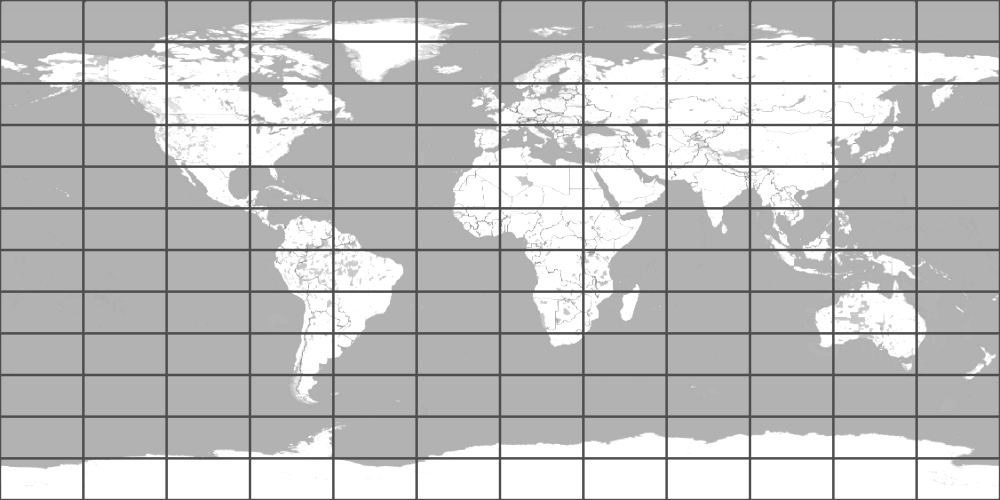
\includegraphics[width=0.9\tw]{projection-platecarree.png}
        \caption{Плоская прямоугольная проекция}
        \label{pic:map-projection-plate-carree}
    \end{subcaptionblock}
    \hfill
    \begin{subcaptionblock}[b]{0.49\tw}
        \centering
        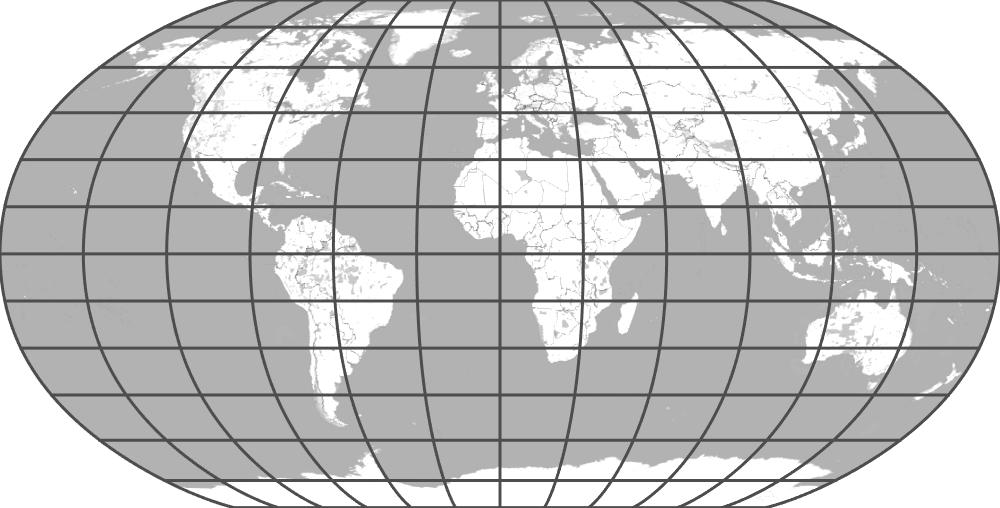
\includegraphics[width=0.9\tw]{projection-robinson.png}
        \caption{Проекция Робинсона}
        \label{pic:map-projection-plate-robinson}
    \end{subcaptionblock}
    \\
    \begin{subcaptionblock}[b]{0.49\tw}
        \centering
        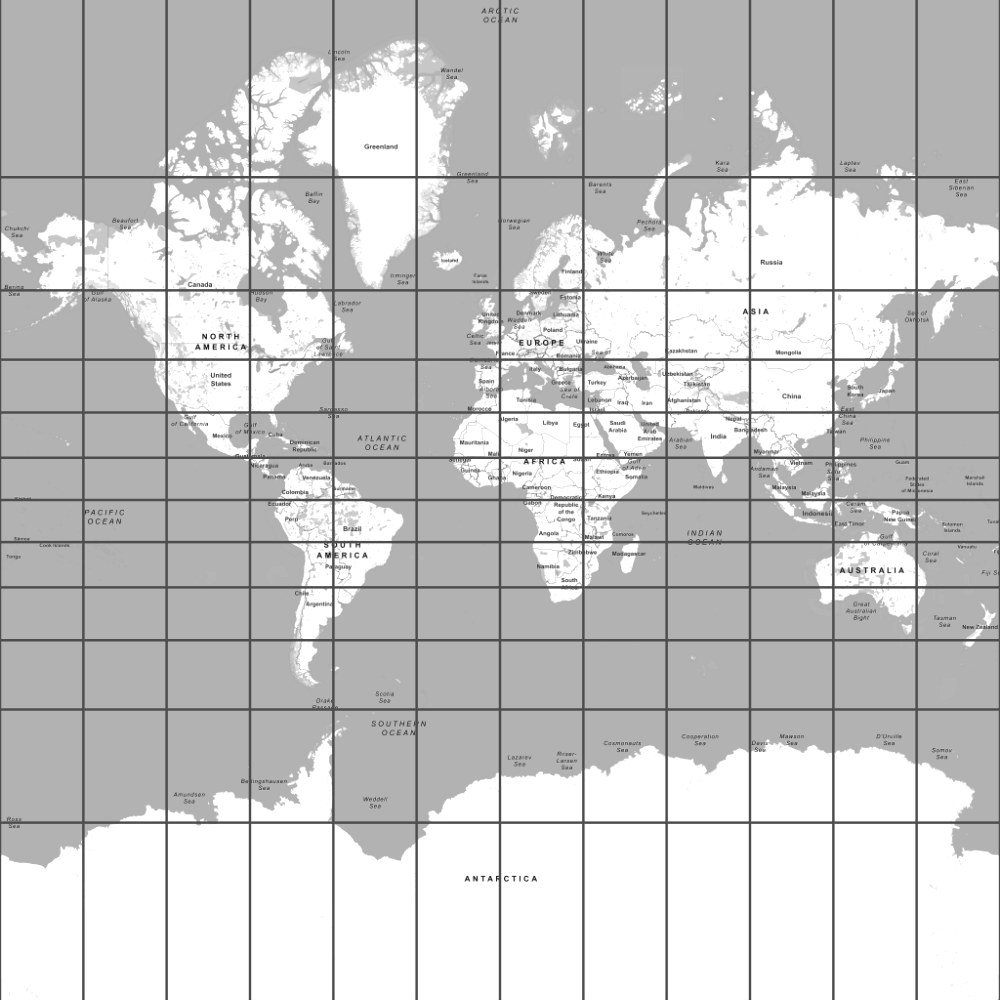
\includegraphics[width=0.9\tw]{projection-mercator.png}
        \caption{Проекция Меркатора}
        \label{pic:map-projection-mercator}
    \end{subcaptionblock}
    \hfill
    \begin{subcaptionblock}[b]{0.49\tw}
        \centering
        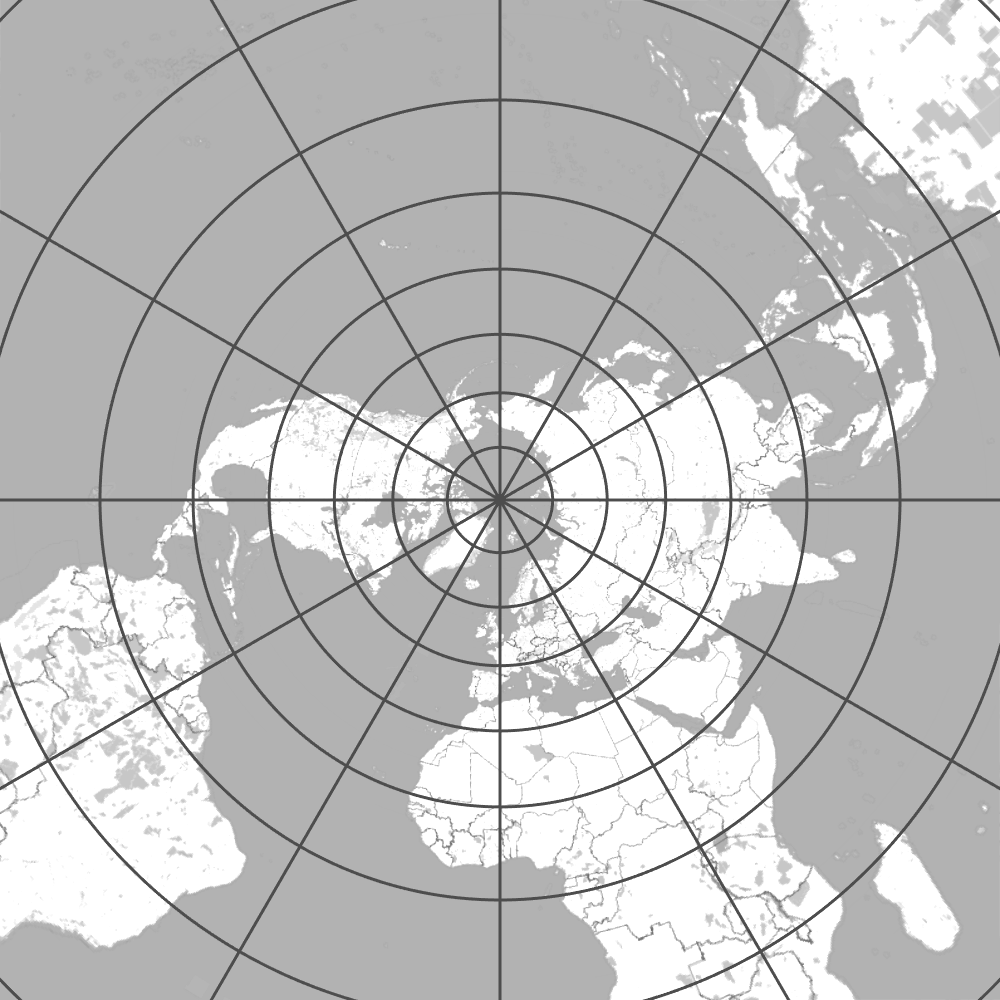
\includegraphics[width=0.9\tw]{projection-stereographic.png}
        \caption{Стереографическая проекция}
        \label{pic:map-projection-stereographic}
    \end{subcaptionblock}
    \\
    \begin{subcaptionblock}[b]{0.49\tw}
        \centering
        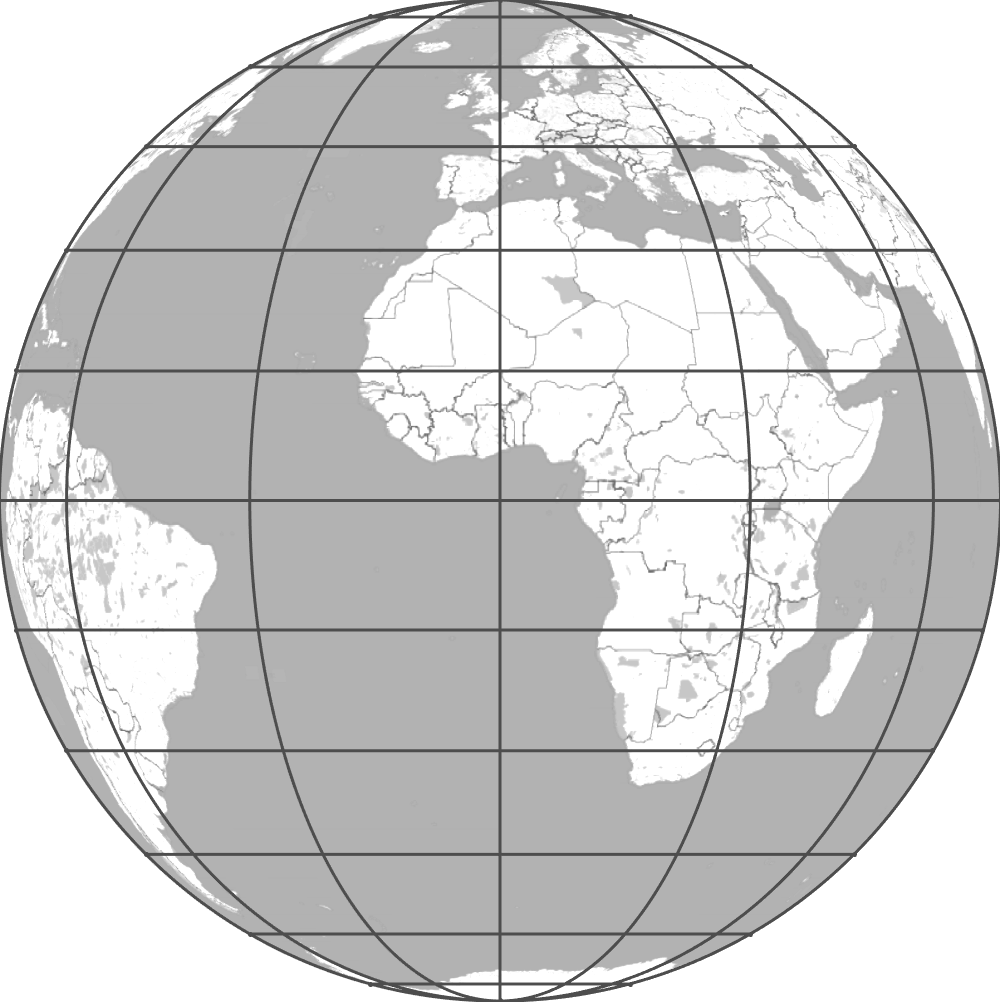
\includegraphics[width=0.9\tw]{projection-orthographic.png}
        \caption{Ортографическая проекция}
        \label{pic:map-projection-orthographic}
    \end{subcaptionblock}
    \hfill
    \begin{subcaptionblock}[b]{0.49\tw}
        \centering
        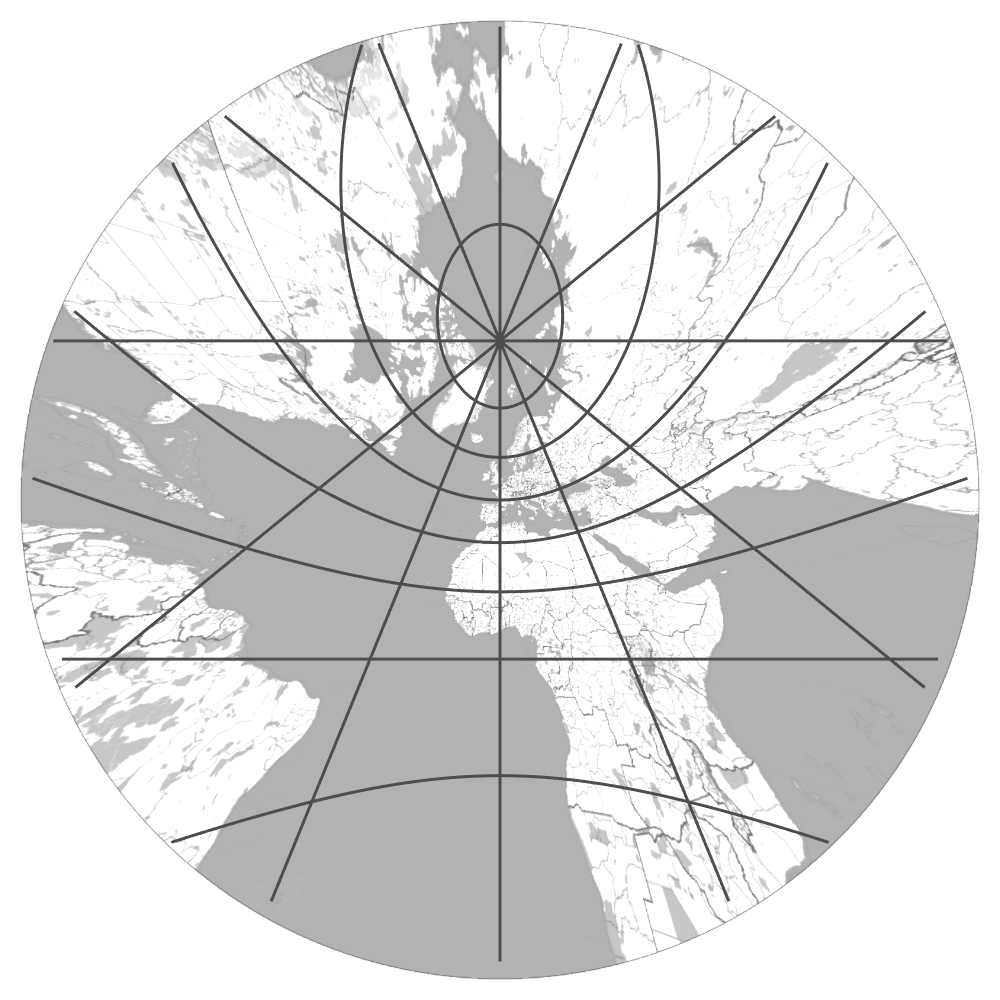
\includegraphics[width=0.9\tw]{projection-gnomonic.png}
        \caption{Гномоническая проекция}
        \label{pic:map-projection-gnomonic}
    \end{subcaptionblock}
    \\
    \begin{subcaptionblock}[b]{0.49\tw}
        \centering
        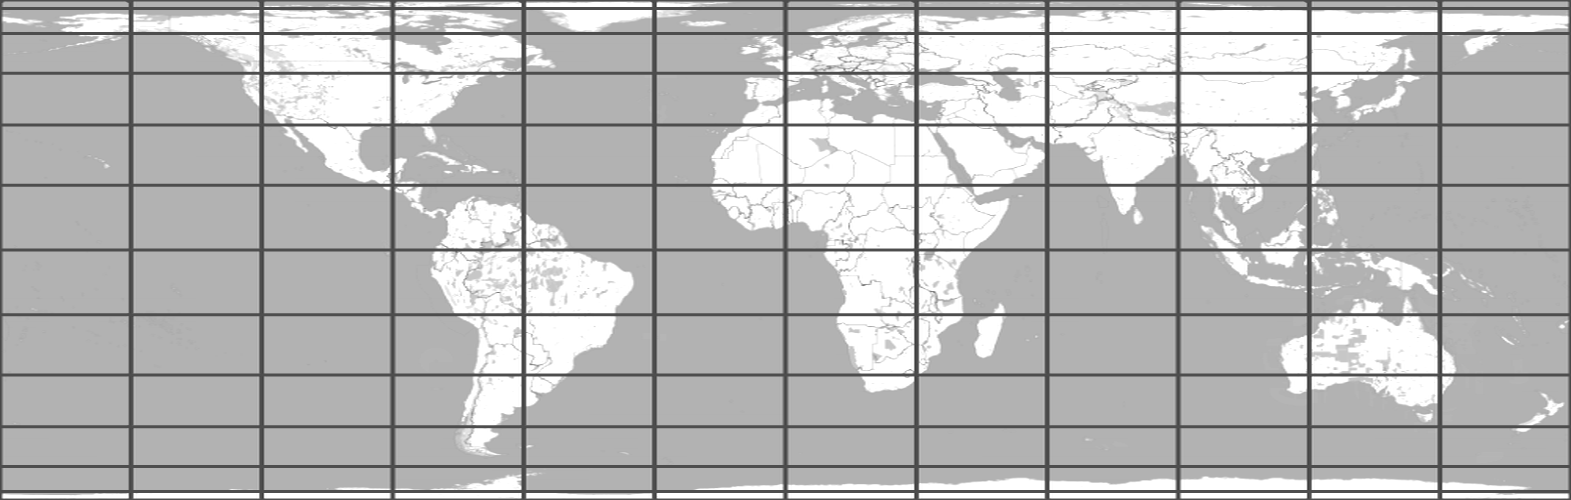
\includegraphics[width=\tw]{projection-lambertcylindrical.png}
        \caption{Цилиндрическая проекция Ламберта}
        \label{pic:map-projection-lambertcylindrical}
    \end{subcaptionblock}
    \caption{Картографические проекции}
    \label{pic:map-projection}
\end{figure}

	\section{Небесная механика}
\subsection{Закон всемирного тяготения}
Согласно \imp{закону всемирного тяготения}, опубликованному в 1687 году Ньютоном в его книге <<Математические начала натуральной философии>>, сила притяжения между двумя точечными телами с массами $M$ и $m$, находящимися на расстоянии $r$, равна
\begin{equation}
	F=\frac{GMm}{r^2}, 
	\label{eq:grav-law-1}
\end{equation}\nopagebreak где $G\simeq 6.67\cdot 10^{-11}~\text{м}^3 /\left( \text{кг} \cdot \text{с}^2 \right)$~---  \term{гравитационная постоянная}, действует вдоль прямой, соединяющей тела, и направлена в сторону гравитирующего тела.

Пусть радиус-вектор $\vec r$ одного тела откладывается от второго, тогда в векторной форме сила, действующая на первое тело,
\begin{equation}
	\vec F (\vec r) = -\frac{GMm}{r^3} \vec r. 
	\label{eq:grav-law-2}
\end{equation}

Векторное поле $\vec V (\vec r)$ называется \term{потенциальным}, если существует такая функция $\varphi(\vec r)$, что $\vec V (\vec r) = - \nabla \varphi(\vec r)$. Рассмотрим векторное поле гравитационых сил~\eqref{eq:grav-law-2}, оно является сферически симметричным, так как зависит только от расстояния до гравитирующего тела, следовательно
\begin{equation*}
	\vec F (\vec r) = -m \frac{d\varphi(r)}{dr} \, \frac{\vec{r}}{r}
\end{equation*} 
%\begin{multline*}
%    \vec F(\vec r) = - m \nabla \varphi(\vec r) = - m \left( \frac{\partial \varphi(\vec r)}{\partial x} \vec e_x + \frac{\partial \varphi(\vec r)}{\partial y} \vec e_y + \frac{\partial \varphi(\vec r)}{\partial z} \vec e_z \right) = \\
%    - m \left( \frac{\,d \varphi(\vec r)}{\,d r} \frac{\partial r}{\partial x} \vec e_x + \frac{\partial \varphi(\vec r)}{\partial y} \vec e_y + \frac{\partial \varphi(\vec r)}{\partial z} \vec e_z \right) =
%\end{multline*}

Перейдём к скалярным величинам, разделим переменные и проинтегрируем левую и правую часть полученного равенства.
%При интегрировании на интервале $(0, r]$ интеграл расходится, поэтому интегрирование будем вести на интервале $(+\infty, r]$, на котором интеграл сходится.
\begin{gather*}
	\int\limits_{+\infty}^{r} \frac{ F(r) }{m} \,d r = \int\limits_{+\infty}^{r} d\varphi(r),\\
%	\int\limits_{+\infty}^{r} \frac{GM }{r^2} \,d r = \int\limits_{+\infty}^{r} d\varphi(r),\\
	-\left.\frac{GM}{r}\right|_{+\infty}^r = \varphi(r)|_{+\infty}^r,\\
	-\frac{GM}{r} + 0 = \varphi(r) - \varphi(+\infty),\\
	\varphi(r) = -\frac{GM}{r} + \varphi(+\infty).
\end{gather*} 
Видно, что потенциал гравитационного поля определен с точностью до постоянной величины $\varphi(+\infty)$, которую для удобства полагают равной нулю. Окончательно, \term{потенциал} гравитационного поля
\begin{equation}
	\varphi(r) = -\frac{GM}{r}.
\end{equation}

\term{Потенциальная энергия} $U(r)$ тела с массой $m$ в гравитационном поле тела с массой $M$~--- энергия, необходимая, чтобы переместить первое тело с бесконечности на расстояние $r$ от второго. Исходя из определения, потенциальная энергия определяется, как
\begin{equation}
	U(\vec r)
	= \oint\limits_{+\infty}^\vec{r} \big(\vec F( \vec r),d \vec r\big) 
	= \int\limits_{+\infty}^r \frac{GMm}{r^2} \,d r 
%	= GMm \left(-\frac{1}{r} + 0 \right) 
	= -\frac{GMm}{r} = U(r).	
\end{equation}

Напряженность гравитационного поля $g$ называют \term{ускорением свободного падения} $g$, вычисляется по формуле
\begin{equation}
	\vec g(\vec r) = -\nabla \varphi(\vec r) = \frac{\vec F( \vec r)}{m} = - \frac{GM}{r^3} \vec r.
	\label{eq:g}
\end{equation} 
Следовательно, (\ref{eq:grav-law-1}) можно записать как
\begin{equation}
	\vec F (\vec r) = m \vec g(\vec r).
\end{equation}

\subsection{Круговое движение. Первая космическая скорость}

Пусть тело движется по окружности радиуса~$R$ с~постоянной скоростью~$v$. Найдём, какой ускорение $\vec a$ оно испытывает в ходе такого движения. Рассмотрим для этого малый промежуток времени $dt$. За это время тело проходит по орбите $d\alpha = \omega \, dt$~радиан, где $\omega$~--- угловая скорость движения тела по окружности, определяемая выражением
\begin{equation*}
    \omega = \frac{2 \pi}{T} = \frac{ 2\pi \cdot v}{2\pi R} = \frac{v}{R},
\end{equation*}
где за $T$ обозначен период движения тела по окружности.

С другой стороны за время $dt$ вектор скорости $\vec{v}$ изменяется на~$d \vec{v}$, причем~$d \vec{v}$ направлен вдоль радиуса окружности в сторону центра. Из~\picRef{pic:circular-velocity} видно, что $d v = v \omega \, dt$, следовательно, модуль ускорения
\begin{equation*}
    a = \frac{dv}{dt} = \omega v = \frac{v^2}{R},
\end{equation*}
а вектор $\vec a$ направлен радиально к центру.

При круговом движении малого тела в гравитационном поле массивного тела массы $M$ первое испытывает силу всемирного тяготения со стороны второго. А значит, оно испытает ускорение свободного падения~$\vec{g}$~\eqref{eq:g}. Приравняв которое к центростремительному ускорению~$\vec{a}$, получим выражение для \term{первой космической} или \term{круговой скорости}.
\begin{gather}
    g = \frac{G M}{R^2} = \frac{v_1^2}{R},\nonumber\\
    v_1 = \sqrt{\frac{GM}{R}},
\end{gather}
где $v_1$~--- первая космическая скорость~--- скорость малого тела на круговой орбите радиуса $R$ вокруг тела массы $M$.

\subsection{Закон сохранения энергии и типы орбит}
Для движения тела c массой $m$ в гравитационном  в поле тела
с массой \linebreak $M\gg m$ со скоростью $v$ на расстоянии $r$ от
гравитационного центра справедливо следующее соотношение:
\begin{equation}
	\frac{m v^2}{2}-\frac{GM m }{r}=E_0,
\end{equation}
где $E_0$~--- величина, равная сумме кинетической и потенциальной энергии тела. Она постоянна, если на тело не действуют внешние силы, кроме силы притяжения к центральному телу. Данное равенство принято называть \term{законом сохранения энергии} для тела, движущегося в поле консервативных (потенциальных) сил.

\begin{wrapfigure}[10]{l}{.5\tw}
	\centering
	\vspace{-1pc}
	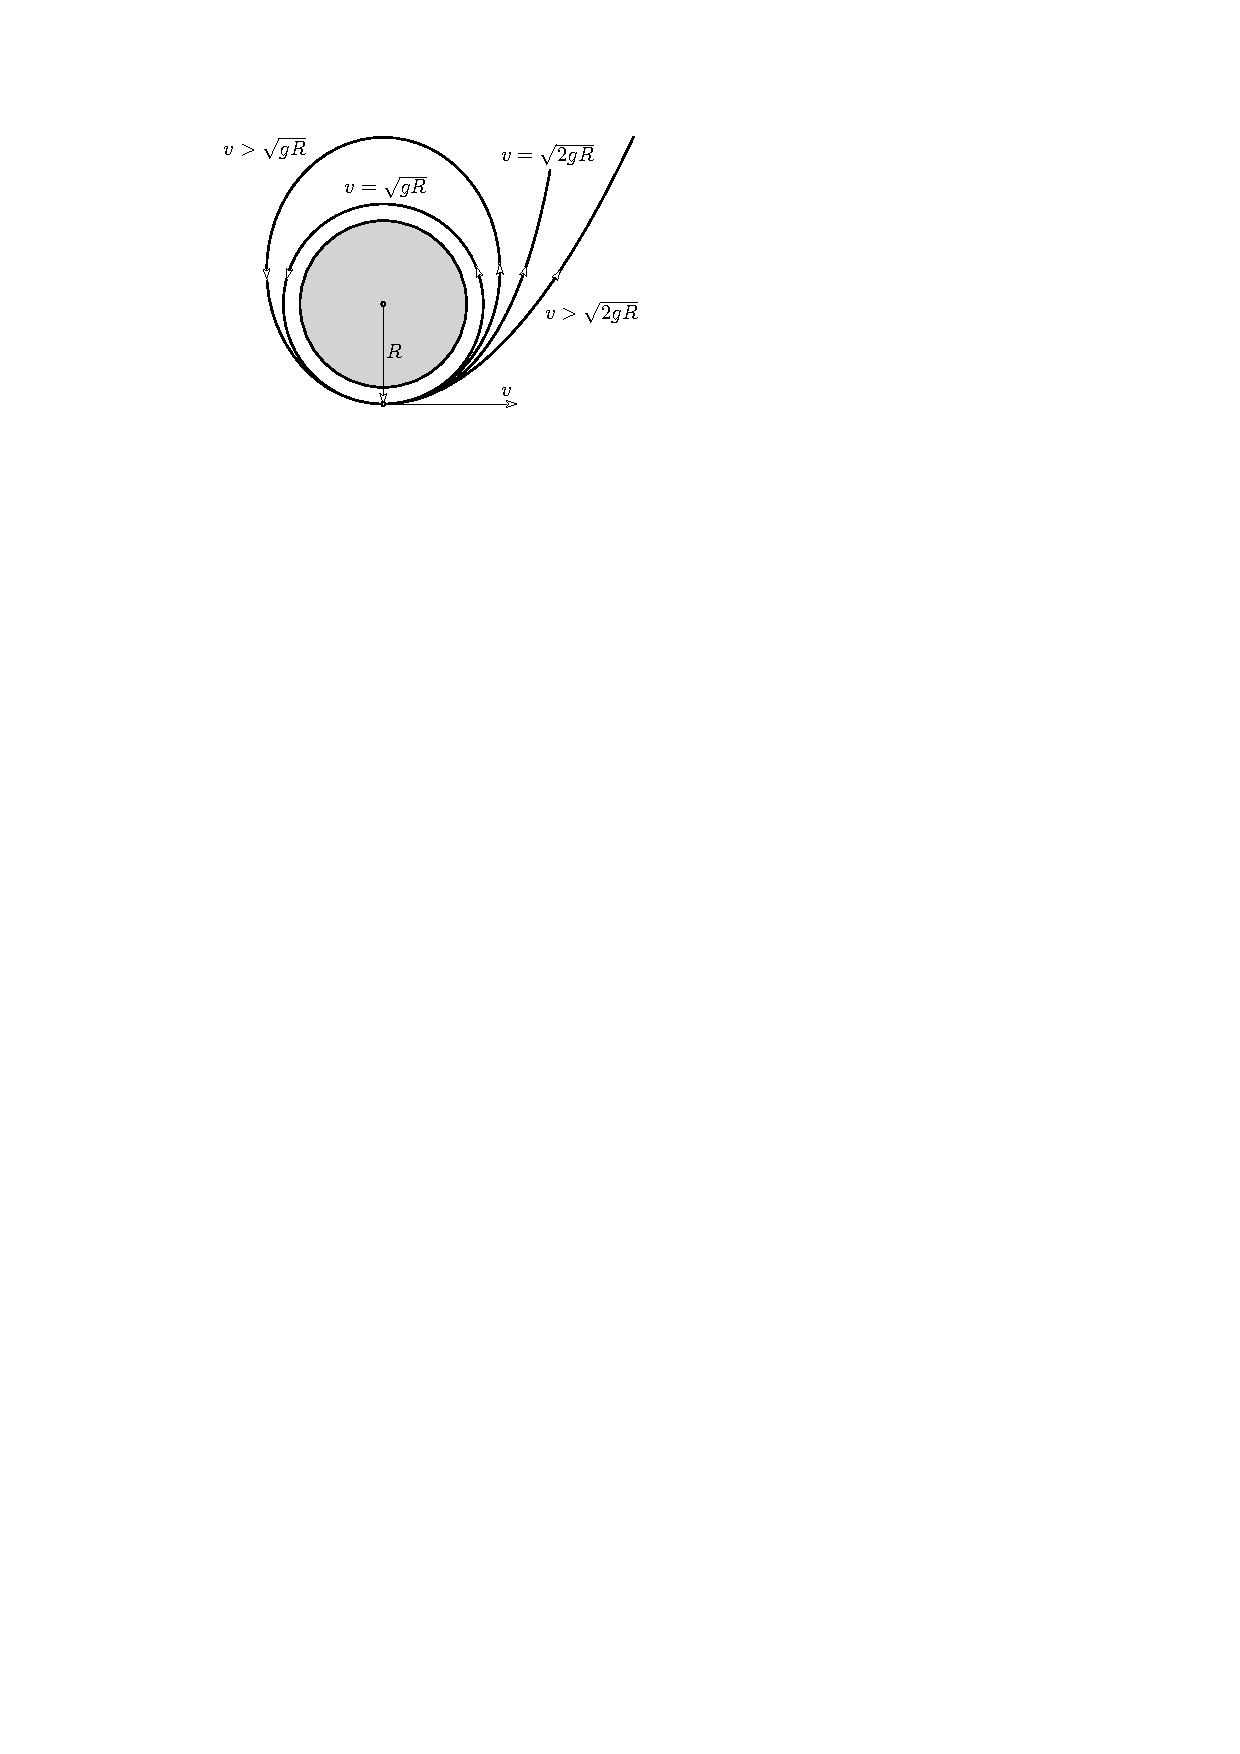
\includegraphics[width = 0.45\tw]{speeds}
	\caption{Возможные траектории тела \label{pic:orbits}}
\end{wrapfigure}
Если $E_0>0$, то траектория тела~--- \imp{гипербола},
ветви которой асимптотически приближаются к двум прямым. Стоит заметить,
что на бесконечно большом удалении малого \linebreak тела от массивного
его скорость остается положительной, так как суммарная энергия $E_0$
больше нуля.

Если $E_0=0$, то траектория тела~--- \imp{парабола}. При стремлении
расстояния $r$ между телами к бесконечности скорость тела с стремится к нулю.

Отсюда становится очевидно, что при параболической и гиперболической
траекториях движение тела не ограничено (инфинитно).

Если $E_0<0$, то траектория тела~--- \imp{эллипс}. При
эллиптической траектории движение ограничено (финитно), так как малое тело
не может бесконечно удаляться по причине того,
что суммарная энергия меньше нуля.

На Рис.\,\ref{pic:orbits} представлены примеры возможных траекторий малого тела
относительно центрального (точка C). При $v_0 > v_{2}$ тело движется
по гиперболе, при $v_0 = v_{2}$~--- по параболе,
а при $v_0 < v_{2}$~--- по эллипсу.

\term{Первая космическая скорость} --- минимальная скорость, необходимая для
того, чтобы маломассивное тело стало искусственным спутником центрального тела.
\begin{equation}v_1=\sqrt{\frac{GM}{R}},
\end{equation}
где $M$ --- масса центрального тела, а $R$~--- радиус орбиты. Отсюда несложно получить выражение для
скорости искусственного небесного тела на высоте~$h$ над~поверхностью тела радиуса $r_0$:
\begin{equation}
	v_h=\sqrt{\frac{GM}{r_0+h}}=\sqrt{\frac{g r_0^2}{r_0+h}}.
\end{equation}

\begin{wrapfigure}[10]{r}{.5\tw}
	\centering
	\vspace{-1pc}
%	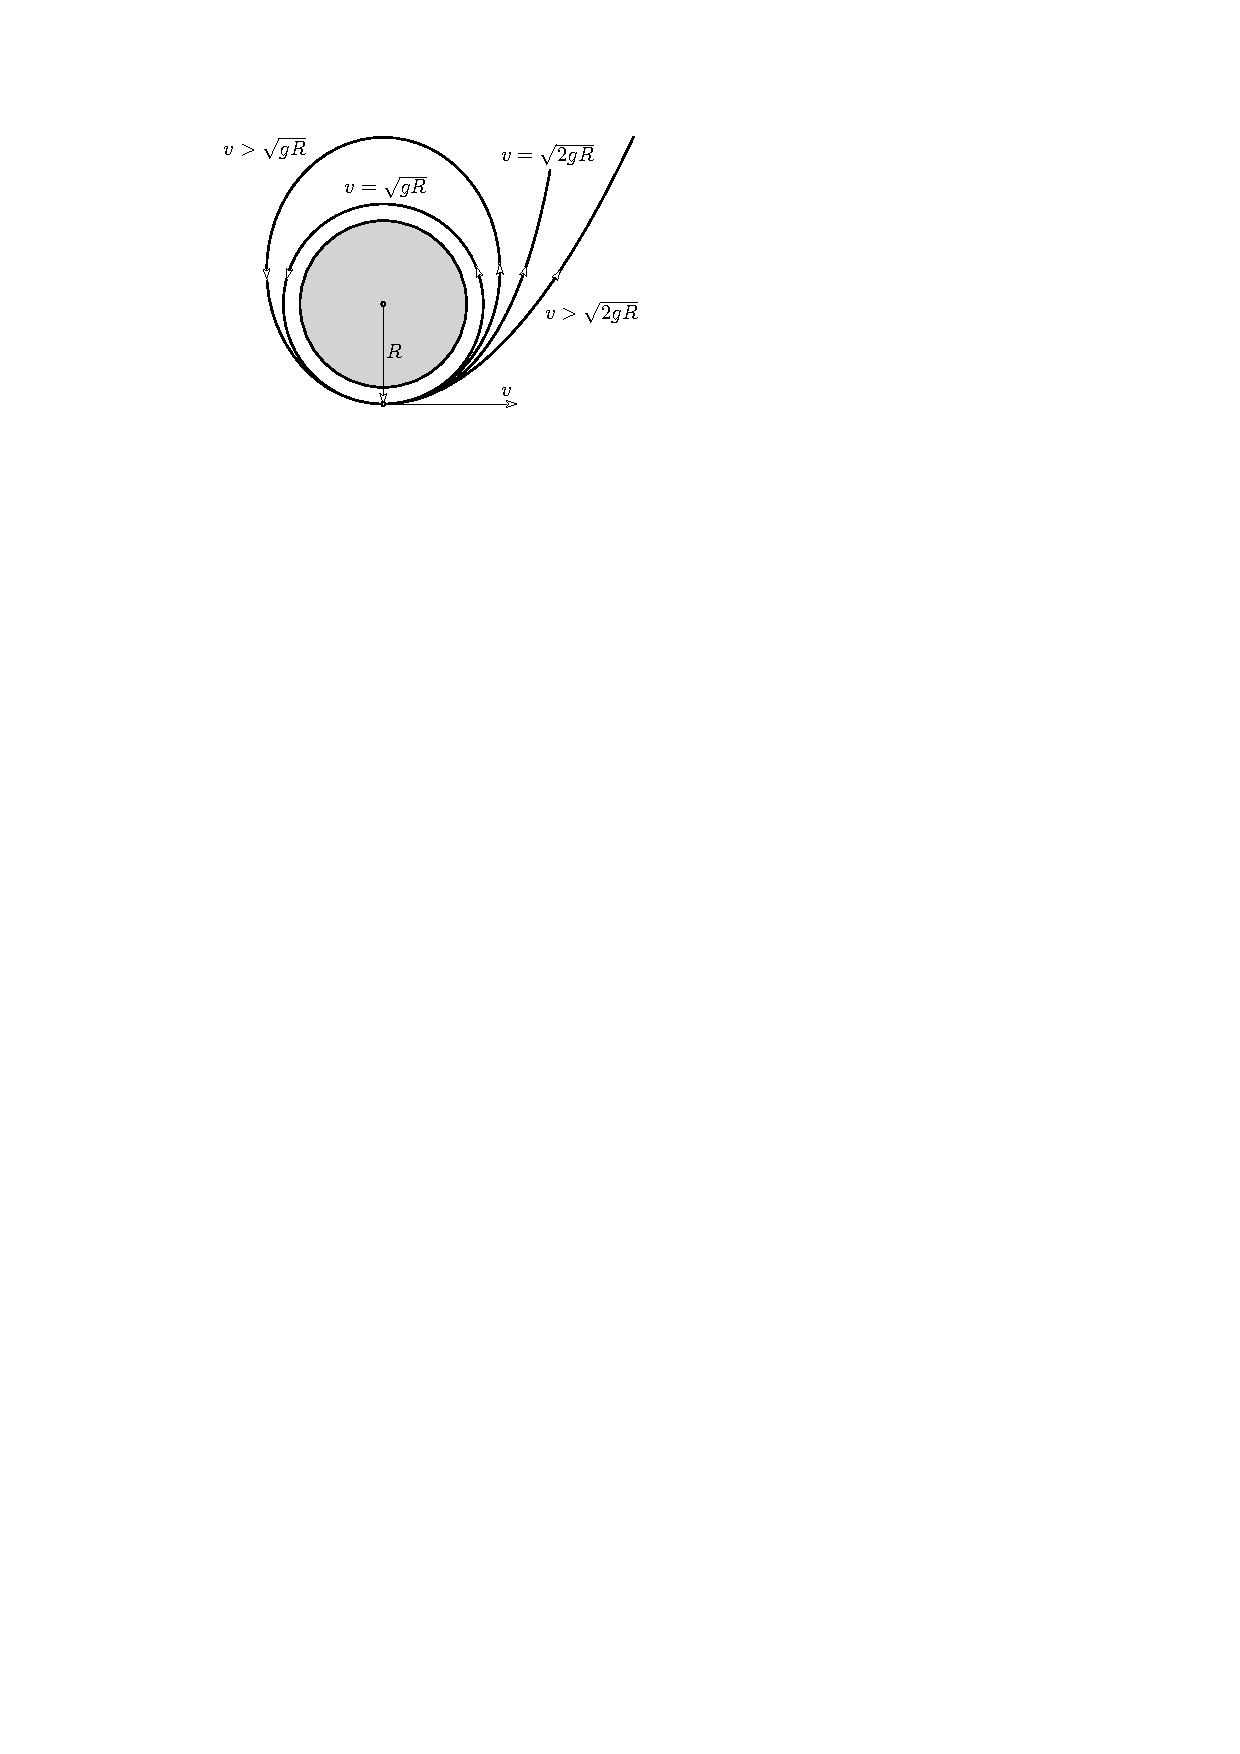
\includegraphics[width=.5\tw]{speeds}
	\caption{Движение по окружности \label{pic:orb-vel}}
\end{wrapfigure}
\change{Вывод:
\\
Рассмотрим 2 точки из траектории ($А$ и $В$) и скорости объекта в этих точках ($v_A$ и $v_B$) соответственно.
\begin{equation}
	\vec{\Delta v} = \vec{v_B} - \vec{v_A}
\end{equation}
При устремлении промежутка времени между пунктами к 0 можно считать, что длина пути становится равна длине хорды $AB$.
\begin{equation}
	\alpha = \frac{\Delta v}{v_A} = \frac{AB}{R}.
\end{equation}
Посчитаем модуль среднего ускорения:
\begin{equation}
	\langle a \rangle = \frac{\Delta v}{\Delta t} = \frac{v \Delta l}{R \Delta t}.
\end{equation}
Перейдя к пределу, получим мгновенное ускорение
\begin{equation}
	a = \lim_{\Delta t \rightarrow 0} \langle a \rangle = \lim_{\Delta t \rightarrow 0} \frac{v \Delta l}{R \Delta t} = \frac{v}{R} \lim_{\Delta t \rightarrow 0} \frac{\Delta l}{\Delta t} = \frac{v^2}{R}.
\end{equation}
Отсюда получаем значение для круговой скорости:
\begin{equation}
	v = \sqrt{a R} = \sqrt{\frac{G M}{R}}.
\end{equation}
}

\term{Параболическая} или \term{вторая космическая скорость} ---
минимальная скорость, необходимая для того, чтобы маломассивное тело преодолело гравитационное притяжение центрального тела, стартуя с расстояния $r$ от его центра масс, и покинуло замкнутую орбиту вокруг
последнего. Выражение для нее имеет следующий вид:
\begin{equation}
	v_{2}=\sqrt{\frac{2GM}{r}}.
\end{equation}
\subsection{Теорема о вириале}
Рассмотрим скалярную функцию механической системы, состоящей из $N$ материальных точек:
\begin{equation}
    V = \sum_{k=1}^N \scalarNoVec{\vec F_k}{\vec r_k},
    \label{eq:virial-def}
\end{equation}
где $\vec r_k$~--- её радиус-вектор $k$-ой материальной точки, а $\vec F_k$~-- равнодействующая сила, действующая на неё. Функция $V$ называется \term{вириалом} системы.

\paragraph{Теорема о вириале} Для стабильной системы материальных точек с установившимся движением~--- положения точек и их скорости ограничены, удвоенная усредненная по времени полная кинетическая энергия равна усредненному по времени вириалу с обратным знаком:
\begin{equation}
    2 \langle T \rangle_\tau = - \langle V \rangle_\tau.
\end{equation}

Приступим к доказательству, 
%пусть $I$~--- момент инерции системы, тогда
%\begin{equation*}
%    I = \sum_{i = 1}^N m_i \vec r_i^2.
%\end{equation*}
%Пусть $T$~--- кинетическая энергия системы, $U$~--- потенциальная, а $\vec F_i$~--- равнодействующая силНайдём первые две производные момента инерции по времени в предположении постоянства масс:
%\begin{equation*}
%    \dot{I} = 2 \sum_{i = 1}^N m_i \scalarNoVec{\vec{r}_i}{\vec{\dot{r}}_i},
%\end{equation*}
%\begin{multline*}
%    \ddot{I} 
%    = 2 \sum_{i = 1}^N m_i \vec{\dot{r}}_i^2 + 2 \sum_{i = 1}^N m_i \scalarNoVec{\vec{r_i}}{\vec{\ddot{r}}_i} 
%    = 2 \sum_{i = 1}^N m_i \vec{v}_i^2 + 2 \sum_{i = 1}^N \scalarNoVec{\vec{r_i}}{\vec{F}_i}    
%\end{multline*}
для удобства введем функцию $Q$:
\begin{equation*}
    Q = \sum_{k=1}^N \scalarNoVec{\vec p_k}{\vec r_k},
\end{equation*}
где $\vec p_k$~--- импульс $k$-ой частицы. Продифференцируем $Q$ по времени:
\begin{equation*}
    \dot Q
    = \sum_{k=1}^N \scalarNoVec{\dot{\vec p_k}}{\vec r_k} 
    + \sum_{k=1}^N \scalarNoVec{\vec p_k}{\dot{\vec r_k}} 
    = \sum_{k=1}^N \scalarNoVec{\vec F_k}{\vec r_k} 
    + \sum_{k=1}^N m_k \scalarNoVec{\dot{\vec r_k}}{\dot{\vec r_k}}
\end{equation*}
Нетрудно заметить, что первое слагаемое в правой части есть вириал, а второе~--- удвоенная кинетическая энергия, следовательно
\begin{equation}
    \dot{Q} = 2T + V.
    \label{eq:virial-2tv}
\end{equation}
Усредним $\dot{Q}$ по времени:
\begin{equation}
    \langle \dot{Q} \rangle_\tau 
    = \frac{1}{\tau} \int\limits_0^\tau \dot{Q} \,d t 
    = \frac{1}{\tau} \int\limits_0^\tau 
    = \frac{Q(\tau) - Q(0)}{\tau}.
\label{eq:virial-avg-g}
\end{equation} 
важно отметить, начало отсчёта времени здесь произвольно.

Функция $Q$ линейно зависит от импульсов и координат точек. Напомним, система стабильна и движения в ней установившиеся. Это означает, что существуют некоторые $\overline Q$, $\underline Q$ и  момент времени $\tau_0$, такие что $\forall \tau > \tau_0:~\underline Q < Q(\tau) < \overline Q$.

Пусть момент начала отсчета времени $\tau = 0$ лежит после $\tau_0$. Тогда очевидно, что $Q(0) > \underline Q$, а $Q(\tau) < \overline Q$, следовательно, $Q(\tau) - Q(0) < \overline Q - \underline Q$, а значит, $|Q(\tau) - Q(0)| < |\overline Q - \underline Q|$, так как $\underline Q < \overline Q$. 

Устремим в \eqref{eq:virial-avg-g} $\tau$ к бесконечности, тогда величина $\langle \dot{Q} \rangle_\tau  \to 0$, так как $\overline Q - \underline Q = \const$, следовательно,
\begin{equation}
    2\langle T \rangle_\tau = - \langle V \rangle_{\tau}.
    \label{eq:virial-t-v}
\end{equation}

Сам по себе вириал в физике встречается не часто. Выше была показана связь вириала с кинетической энергией, найдём теперь связь вириала с ещё одной универсальной величиной~---  потенциальной энергией $U$.\,\cite{virial-theorem}

Равнодействующая сила $\vec F_k$, действующая на $k$-ую точку является суммой сил $\vec F_{ki}$, действующих на $k$-ую точку со стороны всех остальных:
\begin{equation*}
    \vec F_k = \sum_{i \not= k} \vec F_{ki}.
\end{equation*}
Подставим полученное выражение в определение вириала \eqref{eq:virial-def}:
\begin{equation*}
    V = \sum_{k = 1}^N \scalarNoVec{\vec F_k}{\vec r_k}
%    = \sum_{i=1}^N \sum_{k=1}^N \textbf{F}_{ki} \cdot \textbf{r}_{i} 
    = \sum_{k = 1}^N \sum_{i < k} \scalarNoVec{\vec F_{ki}}{\vec r_k}
%    + \sum_{i=1}^N \sum_{k=i} \textbf{F}_{ki} \cdot \textbf{r}_{i} 
    + \sum_{k = 1}^N \sum_{i > k} \scalarNoVec{\vec F_{ki}}{\vec r_k}.
\end{equation*}
Воспользуемся III законом Ньютона: $\vec F_{ki} = - \vec F_{ik}$,
\begin{equation*}
    V = \sum_{k = 1}^N \sum_{i < k} \scalarNoVec{\vec F_{ki}}{\vec r_k}
    - \sum_{k = 1}^N \sum_{i > k} \scalarNoVec{\vec F_{ik}}{\vec r_k}
\end{equation*}
Рассмотрим подробнее второе слагаемое: суммирование ведется по всем $k$ от 1 до $N$ и $i > k$. Это значит, что $i = N$ попадет во все слагаемые первой суммы, $i = N - 1$~--- во все без одного и т.\,д. Следовательно, суммирование можно вести сначала по $i$ от 1 до $N$, а затем по $k < i$. Используем полученный факт, а также поменяем обозначения $k \leftrightarrow i$:
\begin{equation}
    V = \sum_{k = 1}^N \sum_{i < k} \scalarNoVec{\vec F_{ki}}{\vec r_k}
    - \sum_{k = 1}^N \sum_{i < k} \scalarNoVec{\vec F_{ki}}{\vec r_i}
    = \sum_{k = 1}^N \sum_{i < k} \big( \vec F_{ki} \cdot (\vec r_k - \vec r_i) \big).
    \label{eq:virial-v}
\end{equation}

До этого момента не уточнялась природа и вид сил, действующих между частицами. Пусть силы потенциальны, а потенциальная энергия взаимодействия~$U$ зависит от расстояния степенным образом, $U = \gamma r^m$, тогда сила взаимодействия 
\begin{equation*}
    \vec F = -\nabla U = - U'_r \frac{\vec{r}}{r} = -mr^{m - 1} \frac{\vec{r}}{r} = -m r^{m - 2} \vec r.
\end{equation*}
Введем обозначение $\vec r_{ik} \equiv \vec r_k - \vec r_i$ и подставим полученное выражение для силы в~\eqref{eq:virial-v}:
\begin{multline}
    V 
    = \sum_{k = 1}^N \sum_{i < k} \scalarNoVec{\vec F_{ki}}{\vec r_{ik}}
    = \sum_{k = 1}^N \sum_{i < k} -m r_{ik}^{m - 2} \scalarNoVec{\vec r_{ik}}{\vec r_{ik}} = \\
    = \sum_{k = 1}^N \sum_{i < k} -m r_{ik}^{m}
    = -m \sum_{k = 1}^N \sum_{i < k} U_{ik} = -mU,
    \label{eq:virial-v-u}
\end{multline}
где $U_{ik}$~--- потенциальная энергия пары точек $i$ и $k$. Последнее равенство верно, так как в суммировании каждая пара учитывает ровно один раз, а полная потенциальная энергия системы является суммой потенциальных энергий всех пар.

Используя~\eqref{eq:virial-v-u}, перепишем~\eqref{eq:virial-t-v}: 
\begin{equation*}
    2 \langle T \rangle_\tau = m \langle U \rangle_\tau,
\end{equation*} 
для гравитационных сил $m = -1$, отсюда получается важное на практике соотношение, 

\begin{equation}
    \boxed{2\langle T \rangle_\tau = -\langle U \rangle_\tau\!}\,.
\end{equation}

%Пусть все рассматриваемые силы взаимодействия потенциальны. Сила~--- это градиент потенциальной энергии $U$, взятый с обратным знаком. Потенциальная энергия $U$ сферически симметрична, так как зависит только от расстояния между точками, следовательно,
%\begin{equation*}
%    \vec F_{ki} 
%    = -\nabla U_i
%    = - \frac{\partial U_i}{\partial \vec r_{ki}}
%    = -\frac{dU_i}{dr} \frac{\vec{r}_{ki}}{r_{ki}} 
%    = -\frac{dU_i}{dr} \frac{\vec r_k - \vec r_i}{r_{ki}}.
%    \label{eq:virial-f-ki}
%\end{equation*}
%Осталось подставить полученное выражение для $\vec F_{ki}$ в формулу для вириала:
%\begin{equation*}
%\label{V(U)}
%    V 
%    = \sum_{k = 1}^N \sum_{i < k} \scalarNoVec{\vec F_{ki}}{(\vec r_k - \vec r_i)} 
%    = - \sum_{k = 1}^N \sum_{i < k} \frac{dU_i}{dr} \frac{(\vec r_k - \vec r_i)^2}{r_{ki}} 
%    = - \sum_{k = 1}^N \sum_{i < k} \frac{dU_i}{dr} r_{ki}.
%\end{equation*}a
%\paragraph*{Силы, что зависят от расстояния степенным образом}
%Давайте рассмотрим частный случай потенциальной энергии, когда $U(r) \sim r^n$.
%
%В таком случае подставляя $U(r)=\gamma r^n$ в \eqref{V(U)} 
%\begin{equation}
%-V = \sum_{i=1}^N \sum_{k<i} \frac{dU}{dr} r_{ki} = \sum_{i=1}^N \sum_{k<i} n\gamma r_{ki}^{n-1} r_{ki} = \sum_{i=1}^N \sum_{k<i} n\gamma r_{ki}^n.
%\end{equation}
%Заметим, что $\gamma r_{ki}^n = U(r_{ki})$, и тогда используя принцип суперпозиции
%\begin{equation}
%-V = \sum_{i=1}^N \sum_{k<i} nU(r_{ki})=nU.
%\end{equation}
%Теперь вспомним формулу \eqref{eq:virial-t-v} и получим прекрасную формулу
%\begin{equation}
%\label{nice}
%2\langle T \rangle_{\tau} = n\langle U \rangle_{\tau},
%\end{equation}
%но не стоит забывать, что, строго говоря, применима она лишь тогда, когда можно считать что $\langle \dot{Q} \rangle = 0$!
\subsection{Закон сохранения момента импульса}
\term{Момент импульса} ($\vec{L}$)~--- \imp{псевдовекторная} величина, определяющая момент количества движения (импульса). Согласно этому определению момент импульса $\vec{L}$ пробной массы зависит от её радиус-вектора и импульса следующий образом:
\begin{equation}
	\vec{L} = \cross{r}{p}.
\end{equation}

Из геометрического смысла векторного произведения ясно, что $\vec{L}$ ортогонален векторам $\vec{r}$ и $\vec{p}$. Отсюда же $|\vec{L}| \equiv L$ равен площади параллелограмма, построенного на векторах $\vec{r}$ и $\vec p$. Иными словами $L = rp_\perp$, что в свою очередь можно записать как $ L = r p \sin \alpha$, где $\alpha$~--- угол поворота от $\vec{r}$ к $\vec p$, учитывая направление. Согласно свойству векторного произведения, направление $\vec L$ определяется правилом правой руки~--- тройка векторов $\vec r$, $\vec p$ и $\vec L$ должна быть правой.

Для системы пробных масс\footnote{Здесь и далее в этом разделе под пробной массой имеется в виду точечная масса, чтобы не брать в рассмотрение момент импульса вращения тел.}, суммарный момент действия внешних сил на которую равен нулю, полный момент импульса сохраняется. Данное утверждение называется \term[закон сохранения момента импульса]{законом сохранения момента импульса}.

Докажем его сначала в случае движения постоянной пробной массы~$m$ в гравитационном поле неподвижного массивного тела с массой~$M$. Рассмотрим для этого производную по времени момента импульса данной пробной массы:
\begin{multline}
	\frac{d\vec{L}}{dt} = \frac{d\cross{r}{p}}{dt} = \left[ \frac{d \vec{r}}{dt} \times \vec{p} \right] + \left[\vec{r} \times \frac{d\vec{p}}{dt} \right] = m \underbrace{\cross{v}{v}}_{\vec{0}} + \left[\vec{r} \times m \frac{d\vec{v}}{dt} \right] = \\
	= m \cross{r}{a} = m \cross{r}{g(r)} =  -\frac{G M m}{r^3} \underbrace{ \left[\vec{r} \times \vec{r}\right]}_{\vec{0}} = 0.
\end{multline}
Равенство нулю производной момента импульса доказывает его постоянство в рассматриваемом случае.

Обобщим теперь на случай произвольного конечного числа $n$ пробных масс $m_1, \ldots, m_n$:
\begin{multline*}
	\frac{d\vec{L}}{dt} =  \sum\limits_{i=1}^n \frac{d[\vec{r}_i \times \vec{p}_i]}{dt} \overset{m_i=\const}{=} \sum\limits_{i=1}^n \left[\frac{d\vec{r}_i}{dt} \times m_i\vec{v}_i \right] + \sum\limits_{i=1}^n \left[\vec{r}_i \times m_i \frac{d\vec{v}_i}{dt} \right] = \\
	= \sum\limits_{i=1}^n \underbrace{\left[\vec{v}_i \times m_i\vec{v}_i \right]}_{\vec{0}} + \sum\limits_{i=1}^n \left[\vec{r}_i \times m_i \vec{a}_i \right] = \\
	= \sum\limits_{i=1}^n \left[ \vec{r}_i \times m_i \sum\limits_{j=1}^n \frac{G m_j}{|\vec{r}_j - \vec{r}_i|^3} (\vec{r}_j - \vec{r}_i) \right] = \\
	= \sum\limits_{i,j=1}^n \frac{G m_i m_j}{|\vec{r}_j - \vec{r}_i|^3} \big[\vec{r}_i \times (\vec{r}_j - \vec{r}_i) \big] = \sum\limits_{i,j=1}^n \frac{G m_i m_j}{|\vec{r}_j - \vec{r}_i|^3} [\vec{r}_i \times \vec{r}_j] \equiv \sum\limits_{i,j=1}^n \vec{x}_{ij}.
\end{multline*}
Можно заметить, что $\vec{x}_{ij} = -\vec{x}_{ji}$, так как
\begin{equation*}
	\vec{x}_{ij} \equiv \frac{G m_i m_j}{|\vec{r}_j - \vec{r}_i|^3} [\vec{r}_i \times \vec{r}_j] = - \frac{G m_j m_i}{|\vec{r}_i - \vec{r}_j|^3} [\vec{r}_j \times \vec{r}_i] \equiv -\vec{x}_{ji}.
\end{equation*}
Отсюда сразу следует равенство нулю производной по времени полного момента импульса, что завершает доказательство его сохранения.

\begin{figure}[t]
	\begin{subcaptionblock}[b]{0.47\tw}
		\centering
		\begin{tikzpicture}[scale=1.3]
			\footnotesize
			
			\draw [-latex] (0, 0) -- (-2, 0);
			\draw [-latex] (-2, 0) -- (-3, -1);
			
			\draw [dashes, -latex] (-2, 0) -- (-2, -1);
			\draw [dashes] (-2, 0) -- (-3, 0);
			
			\draw (-2.3, 0) arc(180:225:.3);
			\draw (-1.8, 0) -- (-1.8, -.2) -- (-2, -.2);
			
			\draw (0, 0) node {$\odot$};
			
			\point (-2, 0)
			
			\draw (-1, 0) node[anchor=south west] {$\vec{r}$};
			\draw (-2.95, -.9) node[anchor=south] {$\vec{p}$};
			\draw (-2, -.75) node[anchor=west] {$\vec{p}_\perp$};
			\draw (-2.25, -.17) node[anchor=east] {$\alpha$};
			\draw (0, 0) node[anchor=south west] {$\vec{L}$};
			
		\end{tikzpicture}
		\caption{}
	\end{subcaptionblock}
	\hfill
	\begin{subcaptionblock}[b]{0.47\tw}
		\centering
		\begin{tikzpicture}[scale=1]
			\footnotesize
			
			\draw [-latex] (0, 0) -- (0, 2);
			\draw [-latex] (0, 0) -- (2.2, -.6);
			\draw [-latex] (2.2, -.6) -- (3.6, 0);
			\draw [dashes, -latex] (0, 0) -- (1.4, 0.6);
			
			%	\draw [dashes, -latex] (-2, 0) -- (-2, -1);
			\draw [dashes] (2.2, -.6) -- (3, -.82);
			\draw (0, -1) .. controls (2, -1) and (3, -.25) .. (3.5, .4);
			
			\draw (0, .2) -- (.2, 0.15) -- (0.2, -.05);
			\draw (0, .25) -- (.25, 0.35) -- (0.25, .1);
			
			\point (2.2, -.6);
			
			\draw (2.5, -.68) .. controls (2.65, -.6) and (2.65, -.5) .. (2.5, -.47);
			
			\draw (1.1, -.3) node[anchor=south] {$\vec{r}$};
			\draw (3.4, -.1) node[anchor=north] {$\vec{p}$};
			\draw (1.15, 0.55) node[anchor=south] {$\vec{p}$};
			%	\draw (-2, -.75) node[anchor=west] {$\vec{p}_\perp$};
			\draw (2.6, -.55) node[anchor=west] {$\alpha$};
			\draw (0, 1) node[anchor=east] {$\vec{L}$};
			
		\end{tikzpicture}
		\caption{}
	\end{subcaptionblock}
	\caption{}
\end{figure}


\subsection{Эффективный потенцал}

Квадрат скорости тела на орбите массы $m$ может быть выражен как сумма квадратов \imp{лучевой} и \imp{трансверсальной} скоростей. Запишем закон сохранения энергии в следующей форме:
\begin{equation*}
	\frac{m(v^2_r + v^2_{\perp})}{2} - \frac{GMm}{r} = E_0,
\end{equation*}
где $E_0$~--- полная энергия тела на данной орбите. Вспомним выражение для модуля момента импульса:
\begin{equation}
	L = r p_{\perp} = mr v_{\perp}.
\end{equation}
Выразим $v_{\perp}$ через $L$ и подставим в ЗСЭ.
\begin{equation}
	\frac{m v^2_r}{2} + \frac{L^2}{2mr^2} - \frac{GMm}{r} = E_0.
\end{equation}
Эффективным потенциалом системы $\tilde{U}(r)$ называется выражение
\begin{equation}
	\tilde{U}(r) = \frac{L^2}{2mr^2} - \frac{GMm}{r}.
\end{equation}
Рассмотрим случай $v_r=0$ (перицентр или апоцентр орбиты). В таких точках полная энергия тела в точности равна $\tilde{U}(r)$.

\begin{wrapfigure}[10]{r}{0.47\tw}
    \centering
%    \vspace{-1pc}
    \tikzsetnextfilename{effitient-potential-plot}
    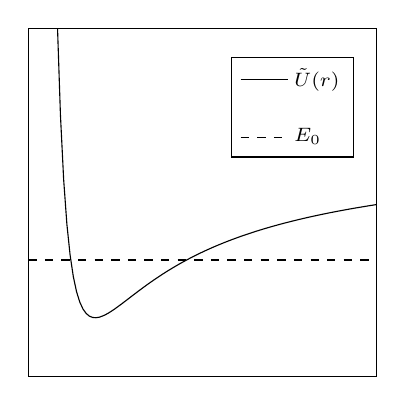
\begin{tikzpicture}
        \begin{axis}[
            width    =    6cm,
            height    =    6cm,
%            xlabel    =    {$r$},
%            xlabel style = {at={(axis description cs:0.5,-0.1)}}
            ymax    =    1,
            ymin    =    -2,
            xmax    =    3,
            xmin    =    0,
            ticks = none,
            legend cell align=left,
            legend style={
                row sep = 0.8pc,
                font=\scriptsize,
                at={(axis cs:1.75, 0.75)}, anchor=north west,
            },
        ]
            \addplot [domain=0.25:3, samples=100, black] {1 / (2 * x^2) - 1.73 / x};
            \addplot [dashed, line width=0.5pt] coordinates { (0,-1) (3,-1) };

            \legend{
                $\tilde{U}(r)$,
                $E_0$
            }
        \end{axis}
    \end{tikzpicture}
    \caption{Эффективный потенциал}
    \label{pic:effitient-potential-plot}
\end{wrapfigure} 

Исходя из \picRef{pic:effitient-potential-plot} при $E_0<0$ существует две различных интересующих нас величины $r$. 
%Так как данные точки соответствуют перицентру и апоцентру орбиты запишем эту пару как $r_{\pi}$ и $r_{\alpha}$ соответственно.
Решим уравнение $\tilde{U}(r) = E_0$, корнями которого являются $r_{\pi}$ и $r_{\alpha}$:
\begin{gather*}
	\frac{L^2}{2mr^2} - \frac{GMm}{r} = E_0 \\
	r^2 + \frac{GMm}{E_0}r - \frac{L^2}{2m E_0} = 0
\end{gather*}
По теореме Виета для корней данного квадратного уравнения можно записать следующие соотношения:
\begin{equation*}
\left\{\begin{aligned}
&r_\pi+r_\alpha=2 a & =-\frac{G M m}{E_0} \\
&r_\pi r_\alpha=b^2 & =-\frac{L^2}{2 m E_0} .
\end{aligned}\right.
\end{equation*}
Решив данную систему уравнений, получим выражения для $E_0$ и $L$:
\begin{gather}
	L = m \sqrt{GMp}, \\
	E_0 = -\frac{GMm}{2a}.
	\label{eq:total-orbit-energy}
\end{gather}








\subsection{Момент инерции}
\label{sec:inertia-moment}

\term{Момент инерции}~--- скалярная\footnote{в общем случае тензорная} величина, определяющая меру инертности тела во вращательном движении, подобна массе в поступательном. Момент инерции характеризует распределение массы в теле и определяется по формуле
\begin{equation}
    I = \int\limits_{V} r^2 \,d m,
\end{equation}
где интегрирование ведется по всему объему тела, а $r$~--- расстояние до оси, относительно которой вычисляется момент инерции.

Так, например, момент инерции однородного шара относительно оси, проходящей через его центр
\begin{multline*}
    I_\text{ш} = \int\limits_0^R \int\limits_{-\sqrt{R^2 - r^2}}^{\sqrt{R^2 - r^2}} \int\limits_0^{2\pi} r^3 \rho \,dr \,dh \,d\varphi 
    = 2\pi \rho \int_0^R \int\limits_{-\sqrt{R^2 - r^2}}^{\sqrt{R^2 - r^2}} r^3 \,dr \,dh = \\
    = 4\pi \rho \int\limits_0^R r^3 \sqrt{R^2 - r^2} \,dr
    \overset{x = R^2 - r^2}{=} -2\pi \rho \int\limits_{R^2}^0 (R^2 - x) \sqrt{x} \, dx = \\
    = - 2\pi \rho R^2 \cdot \left. \frac{2}{3}  x^\frac{3}{2} \right|_{R^2}^0 + 2\pi \rho \cdot \left. \frac{2}{5} x^\frac{5}{2} \right|_{R^2}^0
    = \frac{8}{15} \pi R^5 \rho = \frac{2}{5} m R^2.
\end{multline*}

Пусть $\boldsymbol{\omega}$~--- вектор угловой скорости вращения тела вокруг выделенной оси, тогда секториальная скорость точек тела, расположенных на расстоянии $r$ от оси, $\vec{s} = \boldsymbol{\omega} r^2$. Следовательно, момент импульса вращения 
\begin{equation*}
    \vec{L}_\text{вр} = \int\limits_{V} \boldsymbol{\omega} r^2 \,d m = I\boldsymbol{\omega}.
\end{equation*}

Получаем простую аналогию между поступательным и вращательным движением:
$m \longmapsto I$, $\vec v \longmapsto \boldsymbol\omega$, $\vec{p} \longmapsto \vec{L}$, $\vec F \longmapsto \vec M$, где $\vec{M}$~--- момент силы, определяемый как $\vec{M} = \cross{r}{F}$.

\subsection{Движение по орбите}

\begin{wrapfigure}[8]{r}{0.4\tw}
    \centering
    \vspace{-0.75pc}
    \tikzsetnextfilename{orbit-motion}
    \begin{tikzpicture}
        \def\R{4}
        \def\w{1}
        \def\s{1.5}
        \def\r{2.5}
        \def\eps{0.1}
        
        \tkzDefPoint(0,0){O}
        \tkzDefPoint(0,\w){W}
        \tkzDefPoint(0,\s){S}
        \tkzDefPoint(2.4,-0.6){R1}
        \tkzDefPoint(3,1){R2}
        
        \tkzGetPointCoord(R1){r}
        \tkzGetPointCoord(R2){rr}
        
        \draw [black] plot [smooth, tension=1] coordinates { (0.5,-1) (\rx,\ry) (\rrx,\rry) (4,1.2)};
        
        \tkzDrawSegments[-latex,semithick](O,W O,S O,R1 O,R2 R1,R2)
        
        \tkzLabelPoint[below left = -1pt](W){$\boldsymbol{\omega}$}
        \tkzLabelPoint[below left = -1pt](S){$\vec{s}$}
        \tkzLabelSegment[below](O,R1){$\vec{r}$}
        \tkzLabelSegment[above=1pt](O,R2){$\vec{r}(t + dt)$}
        \tkzLabelSegment[left](R1,R2){$d\vec{r}(t)$}
        
        \tkzMarkRightAngle[size=0.2](R1,O,W)
        \tkzMarkRightAngle[size=0.3](R2,O,W)
        
        \tkzMarkAngle[size=0.4, angle eccentricity=2](R1,O,R2)
        \tkzLabelAngle[pos=0.8](R1,O,R2){\footnotesize$\boldsymbol{\omega} \, dt$}
        
        \tkzDrawPoints(O, R1, R2)
    \end{tikzpicture}
    \caption{}
\end{wrapfigure}
Рассмотрим такую физическую величину, как \term{секториальная ско\-рость}~--- это векторная величина, описывающая ориентированную площадь, заметаемую радиус вектором тела за единицу времени. Пусть в момент времени $t$ тело находилось в точке $\vec{r}(t)$, а через промежуток времени $dt$~--- в точке $\vec{r}(t + dt)$. Обозначим перемещение тела за этот промежуток времени как $d\vec{r}$. Его можно выразить через скорость тела в момент времени $t$, считая её постоянной на промежутке от $t$ до $t + dt$: $d\vec{r} = \vec{v} \,d t$. Площадь, которую заметает радиус-вектор тела $\vec{r}(t)$ равна половине параллелограмма, построенного на векторах $\vec{r}(t)$ и $d\vec{r}$, то есть
\begin{equation*}
    \vec{s} = \frac{1}{2} [\vec{r} \times \vec{v} dt],
\end{equation*}
следовательно, секториальная скорость
\begin{equation*}
    \boldsymbol{\sigma} = \frac{d \vec{s}}{dt} = \frac{1}{2} [\vec{r} \times \vec{v}]  = \frac{\vec{L}}{2m} = \frac{\vec{l}}{2},
\end{equation*}
где $\vec{l}$~--- удельный (на единицу массы) момент импульса. Полученное выражение доказывает \imp{второй закон Кеплера}.

С другой стороны, перемещение $d\vec{r}$ можно выразить через угловую скорость $\boldsymbol{\omega}$, как $d \vec{r} = [\vec{r} \times \boldsymbol{\omega} \,d t]$. Тогда
\begin{equation*}
    \boldsymbol{\sigma}
    = \frac{1}{2} \big[ \vec{r} \times [\vec{r} \times \boldsymbol{\omega} ]\big]
    = \frac{1}{2} \left(\vec{r} \underbrace{(\vec{r}, \boldsymbol{\omega})}_0 - \boldsymbol{\omega} ( \vec{r}, \vec{r} ) \right)
    = \frac{r^2 \boldsymbol{\omega}}{2}.
\end{equation*}

Получим еще одно важное соотношение~--- \term{интеграл энергии}~--- формулу для скорости тела на орбите с большой полуосью $a$ в точке, удалённой на расстояние~$r$ от центрального тела с массой $M$. Для этого рассмотрим  сначала точку перицентра ($q$, <<п>>) и апоцентра ($Q$, <<a>>) данной орбиты. Запишем для них закон сохранения энергии и закон сохранения момента импульса:
\begin{gather*}
    -\frac{GMm}{q} + \frac{m v^2_\text{п}}{2} = -\frac{GMm}{Q} + \frac{m v^2_\text{а}}{2},\\
    mv_\text{п}q = mv_\text{a}Q.
\end{gather*}
Из ЗСМИ и выражений для перицентрического~$q$ и апоцентрического~$Q$ расстояний через большую полуось $a$ и эксцентриситет $e$ имеем:
\begin{equation*}
    \frac{v_\text{а}}{v_\text{п}} = \frac{1 - e}{1 + e}.
\end{equation*}
Используя это соотношения, преобразуем ЗСЭ:
\begin{gather}
    \frac{v_\text{п}^2}{2} \left( 1 - \frac{(1 -e)^2}{(1 + e)^2} \right) = GM \left( \frac{1}{a(1-e)} - \frac{1}{a(1+e)} \right),\\
    \frac{v_\text{п}^2}{2} \cdot \frac{ 1 + 2e + e^2 - 1 + 2e - e^2}{(1+e)^2} = \frac{GM}{a} \cdot \frac{1 + e - 1 +  e}{(1+e)(1-e)},\\
    v_\text{п} = \sqrt{\frac{GM}{a}}\sqrt{\frac{1+e}{1-e}}, \quad \quad v_\text{a} = \sqrt{\frac{GM}{a}}\sqrt{\frac{1-e}{1+e}}.
\end{gather}
Запишем теперь ЗСЭ для перицентра и произвольной точки орбиты на расстоянии $r$:
\begin{gather*}
    -\frac{GMm}{q} + \frac{m v^2_\text{п}}{2} = -\frac{GMm}{r} + \frac{m v^2}{2},\\
    -\frac{GMm}{q} + \frac{GMm}{2a} \cdot \frac{1+e}{1-e} = -\frac{GMm}{r} + \frac{m v^2}{2},\\
    v^2 = GM \left( \frac{2}{r} - \frac{2}{a(1 - e)} + \frac{1+e}{a (1-e) }\right) = GM \left( \frac{2}{r} - \frac{1}{a} \right),
\end{gather*}
\begin{equation}
    v = \sqrt{ GM \left( \frac{2}{r} - \frac{1}{a} \right)}.
    \label{eq:int-energy}
\end{equation}
Полученное выражение и называется интегралом энергии. Согласно \eqref{eq:int-energy} и \eqref{eq:ell-eq-pol} для скорости тела в произвольной точке орбиты также справедливо выражение
\begin{equation}
    v = \sqrt{\frac{GM}{p}\cdot(1 + 2 e \cos \nu + e^2)},
\end{equation}
где $\nu$~--- истинная аномалия, а $p$~--- фокальный параметр.

Установим зависимость скорости от эксцентрической аномалии~$E$\footnote{\lookSecRef{sec:kepler-eq}}, для этого воспользуемся выражением~\eqref{eq:kepler-eq-r-E} и подставим его в интеграл энергии~\eqref{eq:int-energy}, 
\begin{equation}
	v = \sqrt{\frac{GM}{a}}\sqrt{\frac{1 + e \cos E}{1 - e \cos E}}.
	\label{eq:orbit-motion-eccentcic-int-energy}
\end{equation}

Найдем величину момента импульса пробной массы $m$ на эллиптической орбите. В силу постоянства данной величины, можно выбрать любую точку орбиты для её поиска. Проще всего рассмотреть перицентр или апоцентр, рассмотрим первый.
\begin{multline*}
    L
    = m v_q q
    = m \sqrt{\frac{GM}{a} \frac{1+e}{1-e}} \cdot a(1-e) =\\
    = m \sqrt{GMa (1 + e)(1-e)}
    = m \sqrt{GMa(1-e^2)}
    = m \sqrt{GMp}.
\end{multline*}

Для параболической также рассмотрим точку перицентра:
\begin{multline*}
    L
    = m v_q q
    = m v_2(q) q
    = m \sqrt{\frac{2GM}{q}} \cdot q =\\
    = m \sqrt{2GMq}
    = m \sqrt{2GM \cdot \frac{p}{2}}
    = m \sqrt{GMp}.
\end{multline*}
Момент импульса также можно записать в терминах эксцентрической аномалии. Из такого равенства можно получить зависимость угла между радиус-вектором и вектором скорости от эксцентрической аномалии. Записав $L$ как $m r v \sin \alpha$, а далее подставив (\ref{eq:kepler-eq-r-E}) и (\ref{eq:orbit-motion-eccentcic-int-energy})
\begin{gather}
	m a (1 - e \cos E) \cdot \sqrt{\frac{GM}{a}}\sqrt{\frac{1 + e \cos E}{1 - e \cos E}} \sin \alpha = m \sqrt{GMa(1-e^2)}, \nonumber\\
	 \sin \alpha = \sqrt{\frac{1-e^2}{1- e^2 \cos^2 E}}.
\end{gather}


\subsection{Законы Кеплера}
\paragraph{I-ый закон} \imp{Все планеты движутся по
эллиптическим орбитам, в одном из фокусов которых
находится Солнце.}

Для доказательства первого закона Кеплера введём обозначение: $u \equiv 1/r$, используя его, запишем выражение для модуля момента импульса планеты:
\begin{equation*}
	L = 2 m \sigma = m r^2 \omega = \frac{m \omega}{u^2} = \frac{m}{u^2} \frac{d \theta}{d t},
\end{equation*}
где $\theta$~--- угловая координата в полярной системе координат с центром в центре Солнца.
Выразим $dt$ из полученного выражения.
\begin{equation*}
	dt = \frac{m}{L u^2} \,d \theta.
\end{equation*}

Найдем теперь первую производную длины радиус-вектора по времени в новых обозначених:
\begin{equation*}
	\frac{d r}{d t} = \frac{d}{d t} \left( \frac{1}{u} \right) = - \frac{1}{u^2} \frac{du}{dt},
\end{equation*}
подставим сюда выражение для $dt$:
\begin{equation*}
	\frac{d r}{d t} = - \frac{1}{u^2} \frac{du \cdot L u^2}{m \,d \theta} = - \frac{L}{m} \frac{d u}{d \theta}.
\end{equation*}

Далее получим выражение для второй производной:
\begin{equation*}
	\frac{d^2 r}{dt^2} = \frac{d}{dt} \frac{d r}{d t} = \frac{d}{dt} \left( - \frac{L}{m} \frac{d u}{d \theta} \right) = -\frac{L}{m} \frac{d^2 u}{dt \,d \theta},
\end{equation*}
снова воспользуемся выражением для $dt$,
\begin{equation*}
	\frac{d^2 r}{dt^2} = - \frac{L^2	 u^2}{m^2} \frac{d^2 u}{d \theta^2}.
\end{equation*}

Запишем теперь уравнение движения планеты в гравитационном поле Солнца~--- результирующая сила, действующая на планету равна сумме силы гравитационного притяжения и центробежной силы.
\begin{gather}
	m \frac{d^2 r}{d t^2} = - \frac{G M m}{r^2} + m \omega^2 r, \nonumber \\
	- \frac{L^2	 u^2}{m^2} \frac{d^2 u}{d \theta^2} = - GMu^2 + \frac{L^2 u^3}{m^2}, \nonumber\\
	\frac{d^2 u}{d \theta^2} + u = \frac{GM m^2}{L^2}. \label{eq:first-kepler-law-eq}
\end{gather}
Общее решение полученного неоднородного уравнение есть сумма общего решения однородного уравнения 
\begin{equation*}
	\frac{d^2 u}{d \theta^2} + u = 0
\end{equation*}
и частного решения неоднородного уравнения. В качестве частного решения возьмём 
\begin{equation*}
	u(\theta) = \frac{GM m^2}{L^2} = \const.
\end{equation*}
Однородное уравнения является уравнением гармонических колебаний, поэтому его решение можно представить в виде
\begin{equation*}
	u(\theta) = A \cos \theta,	
\end{equation*}
где $A$~--- постоянная интегрирования, определяемая из начальных условий. Общее решение неоднородного уравнения запишется, как
\begin{equation}
	u(\theta) = \frac{GM m^2}{L^2} + A \cos \theta \equiv \frac{1}{r(\theta)}.
	\label{eq:solution-first-kepler-law-eq}
\end{equation}

В качестве начальных условий рассмотрим: $r(0) = s$, $L = m\sqrt{G M h}$, где $s$ и $h$ пока только некоторые расстояния. Подставив выбранные начальные условия в решение~\eqref{eq:solution-first-kepler-law-eq} уравнения~\eqref{eq:first-kepler-law-eq}, получим, что
\begin{gather*}
%	\frac{1}{s} = \frac{GM m^2}{m^2 G M h} + A,\\
	A = \frac{s - h}{sh}.
\end{gather*}
В итоге решение уравнение примет вид
\begin{gather*}
	\frac{1}{r} = \frac{1}{h} + \frac{s - h}{sh} \cos \theta,\\
	r = \frac{sh}{s + (s - h) \cos \theta},\\
	r = \frac{h}{1 + \dfrac{s - h}{s} \cos \theta}.
\end{gather*}
Полученное уравнение является уравнением эллипса в полярных координатах, где $(s - h)/s$~--- эксцентриситет $e$, $h$~--- фокальный параметр $p$, а $\theta$~--- истинная аномалия $\nu$. Это завершает доказательство первого закона Кеплера. Для задачи двух тел доказательство аналогично, достаточно воспользоваться \imp{приведённой массой}.

\paragraph{II-ой закон} \imp{Радиус-вектор планеты за
равные промежутки времени заметает равные площади.}
\begin{equation}
	 \frac{dS}{dt} = \sigma =\frac{L}{2m} = \const = \frac{S_\text{эл}}{T} = \frac{\pi a b }{T}.
\end{equation}
Второй закон Кеплера является прямым следствием \imp{закона сохранения момента импульса}.


\paragraph{III-ий закон} \imp{Квадраты периодов обращения планет
относятся как кубы больших полуосей их орбит.}
\begin{equation}
	\frac{T^2_1}{T^2_2}=\frac{a^3_1}{a^3_2},
\end{equation}
где $a$ --- большая полуось, $T$ --- период обращения.
\begin{figure}[h!]
	\begin{minipage}[b]{0.5\textwidth}
		\centering
		\begin{tikzpicture}
		    \footnotesize
		    
		    \def\padding{0.3}
		    \def\r{2.5}
		    \def\bByA{0.7}
		    
		    \tkzInit[
		          xmin={-\r - \padding},
		          xmax={\r + \padding}, 
		          ymax={\r*\bByA + \padding},
		          ymin={-\r*\bByA - \padding}     
		    ]
		    \tkzClip
		    \begin{scope}[yscale=\bByA]
		    
		      \def\c{\r * sqrt(1 - \bByA^2)}
		      \tkzDefPoint(0,0){O};  
		      \tkzDefPoint(\c,0){F};
		      \tkzDefPointBy[symmetry=center O](F) \tkzGetPoint{F'}
		      \tkzDefPoint(\r,0){Q}
		      \draw[thick] (O) circle (\r cm);
		      
		      \def\planetAngle{120}
		      \tkzDefPointBy[rotation=center O angle \planetAngle](Q) \tkzGetPoint{P}
		      \tkzDrawPoint(P)
		      
		      \def\arrowShiftAngle{15}
		      \tkzDefPointBy[rotation=center O angle \arrowShiftAngle](P) \tkzGetPoint{A'}
		      
		      \def\arrowCoef{1.15}
		      \def\arrowAngularSize{15}
		      \tkzDefPointBy[homothety=center O ratio \arrowCoef](A') \tkzGetPoint{A}
		      \draw[-latex] (A) arc({\planetAngle + \arrowShiftAngle}:{\planetAngle + \arrowShiftAngle + \arrowAngularSize}:{\r * \arrowCoef});
		      

		    \end{scope}
		    \sun(F)
		    \tkzLabelPoint[below](F){Солнце}
		    \tkzLabelPoint[above left](P){Планета}
		    \tkzDrawPoint(F')
		    \tkzLabelPoint[below](F'){$F$}
		\end{tikzpicture}
%		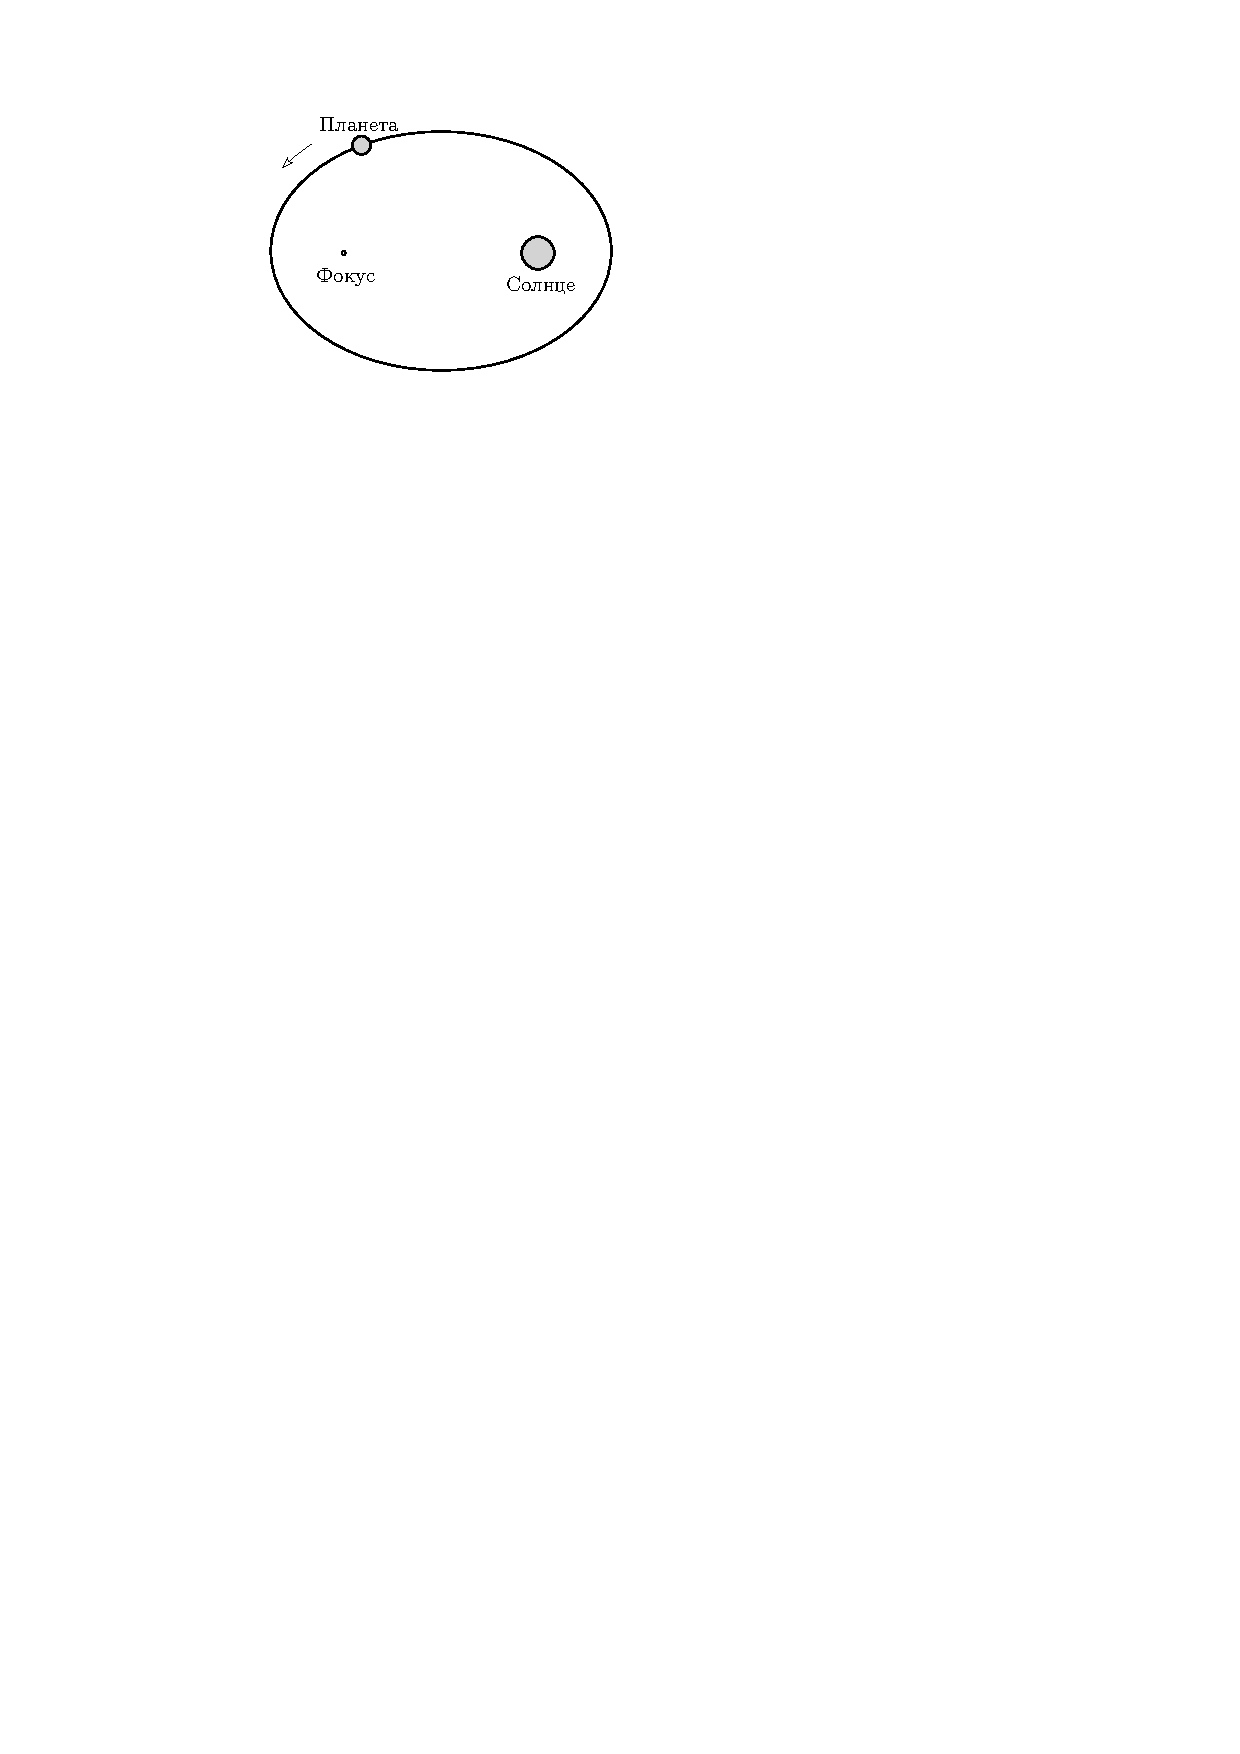
\includegraphics[width = 0.84\textwidth]{first-kepler}
		\caption{Первый закон Кеплера}
	\end{minipage}
	\begin{minipage}[b]{0.5\textwidth}
		\centering
		\begin{tikzpicture}
            
            \def\padding{0.3}
		    \def\r{2.5}
		    \def\bByA{0.7}
		    
		    \tkzInit[
		          xmin={-\r - \padding},
		          xmax={\r + \padding}, 
		          ymax={\r*\bByA + \padding},
		          ymin={-\r*\bByA - \padding}     
		    ]
		    \tkzClip
		    
		    \begin{scope}[yscale=\bByA]
		    
		      \def\c{\r * sqrt(1 - \bByA^2)}
		      \tkzDefPoint(0,0){O};  
		      \tkzDefPoint(\c,0){F};
		      \tkzDefPointBy[symmetry=center O](F) \tkzGetPoint{F'}
		      \tkzDefPoint(-20:\r){A_1};
		      \tkzDefPoint(40:\r){B_1};
		      \tkzDefPoint(120:\r){A_2};
		      \tkzDefPoint(140:\r){B_2};
		      \tkzDefPoint(-120:\r){A_3};
		      \tkzDefPoint(-90:\r){B_3};

		      \draw[thick] (O) circle (\r cm);
		      \draw [fill=lightgray, line width=.4pt] (F) -- (A_1) arc(-20:40:2.5) -- cycle;
		      \draw [fill=lightgray, line width=.4pt] (F) -- (A_2) arc(120:140:2.5) -- cycle;
		      \draw [fill=lightgray, line width=.4pt] (F) -- (A_3) arc(-120:-90:2.5) -- cycle;
		    
		      \tkzDefPointBy[homothety=center O ratio 1.04](A_1) \tkzGetPoint{A_1'}
		      \tkzDefPointBy[homothety=center O ratio 1.05](A_2) \tkzGetPoint{A_2'}
		      \tkzDefPointBy[homothety=center O ratio 1.05](A_3) \tkzGetPoint{A_3'}
		     
		      \tkzDefMidPoint(A_1,B_1) \tkzGetPoint{M_1}
		      \tkzDefMidPoint(A_2,B_2) \tkzGetPoint{M_2}
		      \tkzDefMidPoint(A_3,B_3) \tkzGetPoint{M_3}
		    
		      \tkzDefPointBy[homothety=center O ratio 1.3](M_1) \tkzGetPoint{M_1'}
		      \tkzDefPointBy[homothety=center O ratio 1.2](M_2) \tkzGetPoint{M_2'}
		      \tkzDefPointBy[homothety=center O ratio 1.2](M_3) \tkzGetPoint{M_3'}
		    
		      \draw [latex-latex] (A_1') arc(-20:40:2.6);
		      \draw [latex-latex] (A_2') arc(120:140:2.625);
		      \draw [latex-latex] (A_3') arc(-120:-90:2.625);
		      
		      \tkzLabelPoint(M_1'){$t$}
		      \tkzLabelPoint(M_2'){$t$}
		      \tkzLabelPoint(M_3'){$t$}
		      
		      
		      \tkzDefBarycentricPoint(F=-0.2,A_1=1,B_1=1) \tkzGetPoint{S_1}
		      \tkzLabelPoint(S_1){$S$}
		      \tkzDefBarycentricPoint(F=0.4,A_2=1,B_2=1) \tkzGetPoint{S_2}
		      \tkzLabelPoint(S_2){$S$}
		      \tkzDefBarycentricPoint(F=0.4,A_3=1,B_3=1) \tkzGetPoint{S_3}
		      \tkzLabelPoint(S_3){$S$}
		    \end{scope}
		    \sun(F)
		    \tkzDrawPoint(F')
		    \tkzLabelPoint[below](F'){$F$}
		\end{tikzpicture}
		\caption {Второй закон Кеплера}
	\end{minipage}
\end{figure}

Получим третий закон Кеплера, из второго. Для этого используем выражения для секториальной скорости через площадь эллипса
\begin{equation*}
    \sigma = \frac{\pi a b}{T} = \frac{\pi a^2 \sqrt{1 - e^2}}{T}
\end{equation*}
 и через момент импульса~--- рассмотрим точку перицентра:
\begin{equation*}
    \sigma = \frac{L}{2m} = \frac{m \sqrt{\dfrac{GM}{a} \cdot \dfrac{1 + e}{1 - e}} \cdot a(1-e)}{2m}.
\end{equation*}
Приравнивая их друг другу имеем:
\begin{gather*}
 \frac{\pi a^2 \sqrt{1 - e^2}}{T}
	= \frac{m \sqrt{\dfrac{GM}{a} \cdot \dfrac{1 + e}{1 - e}} \cdot a(1-e)}{2m},\\
	\frac{4\pi^2 a^4 (1 - e^2)}{T^2}
	= a^2(1-e)^2 \cdot \frac{GM}{a} \cdot \frac{1 + e}{1-e}
\end{gather*}
\begin{equation}
	\frac{T^2}{a^3} = \frac{4\pi^2}{GM}.
\end{equation}

\term{Обобщённый} Ньютоном \term{III-ий закон Кеплера} имеет вид:
\begin{equation}
	\frac{T^2_1( M_1 + m_1)}{T^2_2( M_2 + m_2 )}=\frac{a^3_1}{a^3_2} \quad \Leftrightarrow \quad
	\frac{T^2 ( M + m )}{a^3} = \frac{4 \pi^2}{G},
\end{equation}
где $M_1$ и $M_2$~--- массы центральных тел, $m_1$ и
$m_2$~--- массы обращающихся вокруг них тел. Так как характерная масса планеты
$m$ много меньше массы звезды $M$, полагают $M + m \simeq M$.

\subsection{Задача двух тел}
В случае сравнимых масс законы Кеплера нуждаются в уточнении. Данная проблема называется \term{задачей двух тел}. Пусть в пространстве в некоторой произвольной системе отсчета существуют два тела с массми $M_1$ и $M_2$ c данными начальными координатами $\vec{r}_1$ и $\vec{r}_2$, а также начальными скоростями $\vec{v}_1$ и $\vec{v}_2$. Решение задачи двух тел заключается в поиске законов движения $\vec{r}_1(t)$ и $\vec{r}_2(t)$.

\begin{wrapfigure}[7]{r}{0.47\tw}
    \centering
    \vspace{-1pc}
    \tikzsetnextfilename{reduced-mass}
    \begin{tikzpicture}[]
        
        \tkzDefPoint(0, 0){BC}
        \tkzDefPoint(-2, 1){M1}
        \tkzDefPoint(1, -1/2){M2}
        \tkzDefPoint(-1, -1){O}
        
        \tkzLabelPoint[above right](BC){ц.м.}
        \tkzLabelPoint[left](M1){$M_1$}
        \tkzLabelPoint[right](M2){$M_2$}
        \tkzLabelSegment[below left=-3pt](O,M1){$\vec{r_1}$}
        \tkzLabelSegment[below right=-3pt, pos=0.45](O,M2){$\vec{r_2}$}
        \tkzLabelSegment[above, pos=0.45](M1,M2){$\vec{r}$}
        \tkzLabelSegment[above left=-3pt](O,BC){$\vec{R}$}
        
        \tkzDrawSegments[latex-](M1,O M2,O M1,M2 BC,O)
        
        \tkzDrawPoints(M1,M2,O,BC)
    \end{tikzpicture}
    \caption{}
    \label{pic:reduced-mass}    
\end{wrapfigure}

Второй закон Ньютона в данной СО записывается как:
\begin{equation}
\begin{aligned}
	\vec{F}_{12} &= M_1 \ddot{\vec{r}}_1,\\
	\vec{F}_{21} &= M_2 \ddot{\vec{r}}_2.
\end{aligned}
\label{eq:tbp-newton-second-laws}
\end{equation}
Если сложить два данных уравнения, учитывая что по третьему закону Ньютона $\vec{F}_{12} = -\vec{F}_{21}$, можно получить частный случай \imp{теоремы о движении центра масс}:
\begin{equation*}
	M_1 \ddot{\vec{r}}_1 + M_2 \ddot{\vec{r}}_2 = (M_1 + M_2) \ddot{\vec{R}} = 0,
\end{equation*}
где $\ddot{\vec{R}}$~--- ускорение центра масс системы. Данное равенство следует напрямую из определения центра масс. % добавить \ref
Введем вектор $\vec{r}$ как $\vec{r}_1-\vec{r}_2$, тогда общее решение задачи можно найти как:
\begin{equation}
\begin{aligned}
	\vec{r_1}(t) &= \vec{R}(t) + \frac{M_2}{M_1 + M_2} \vec{r}(t), \\
	\vec{r_2}(t) &= \vec{R}(t) - \frac{M_1}{M_1 + M_2} \vec{r}(t).
\end{aligned}
\end{equation}
Как уже было показано, в данной системе ускорение центра масс равно нулю, а его координаты и скорость находятся напрямую из начальных условий, поэтому сконцентрируемся на поиске выражения для $\vec{r}(t)$.

Поделим каждое из уравнений (\ref{eq:tbp-newton-second-laws}) на соответствующую массу и вычтем их друг из друга:
\begin{equation}
	\ddot{\vec{r}}_1 - \ddot{\vec{r}}_2 = \ddot{\vec{r}} = \frac{\vec{F}_{12}}{M_1}-\frac{\vec{F}_{21}}{M_2} = \left(\frac{1}{M_1}+\frac{1}{M_2}\right) \vec{F} = \frac{\vec{F}}{\mu}.
	\label{eq:tbp-relative-second-law}
\end{equation}
Тут мы опять воспользовались третьим законом Ньютона, чтобы обозначить $\vec{F} = \vec{F}_12 = -\vec{F}_21$. Выражение с обратной суммой обратных масс называется \term{приведённой массой} системы.
\begin{equation}
	\mu = \frac{1}{\frac{1}{M_1} + \frac{1}{M_2}} = \frac{M_1 M_2}{M_1 + M_2}.
\end{equation}
Выражение (\ref{eq:tbp-relative-second-law}) является аналогом второго закона Ньютона для задачи двух тел. Это уравнение можно решить аналогично обычной задаче Кеплера и свести его к аналогу уравнения (\ref{eq:first-kepler-law-eq}):
\begin{equation}
	\frac{d^2 u}{d \theta^2} + u = \frac{GM_1 M_2}{\mu l^2}.
\end{equation}
Решение данного уравнения~--- эллипс с фокальным параметром
\begin{equation*}
	p = \frac{\mu l^2}{GM_1 M_2} = \frac{l^2}{G(M_1 + M_2)}.
\end{equation*}
Таким образом тела будут двигаться по подобным эллипсам с коэффициентом подобия $M_1/M_2$ так, что центр масс системы будет двигаться без ускорения.

Найдем выражение для полной энергии в системе двух тел. По определению полная энергия есть сумма кинетической и потенциальной:
\begin{equation*}
	T + U = E_0
\end{equation*}
Из теоремы о вириале известно соотношение
\begin{equation*}
	2\langle T \rangle_\tau = -\langle U \rangle_\tau
\end{equation*}
Таким образом можно получить выражение для полной энергии через среднюю величину потенциальной энергии:
\begin{equation*}
	E_0 = \left\langle \frac{U}{2} \right\rangle_\tau
\end{equation*}
Гравитационный потенциал имеет форму $1/r$. Найдем по определению среднее по времени (средней аномалии) значение величины $1/r$ для тела на орбите:
\begin{equation*}
	\left\langle \frac{1}{r} \right\rangle_\tau = \frac{1}{2 \pi} \int\limits_0^{2\pi}\frac{dM}{r} = \frac{1}{2 \pi} \int\limits_0^{2\pi}\frac{dE}{a} = \frac{1}{a}.
\end{equation*}
Тут мы воспользовались соотношением $a dM = r dE$. Отсюда величина полной энергии
\begin{equation*}
	E_0 = -\frac{G M_1 M_2}{2a},
\end{equation*}
где $a$ есть полуось эллипса образованного вектором $\vec{r}$.






\subsection{Типы орбит}
\label{sec:orbit-types}

Вернемся к первому закону Кеплера, в частности к полученному уравнению орбиты \eqref{eq:first-kepler-law-conic-seq-eq}. Определим, как знак полной механической энергии связан с видом орбиты. 

Заметим, в принятых обозначениях $s$~--- перицентр орбиты, так как истинная аномалия отсчитывается от перицентра, то есть минимальное расстояние от тела до гравитирующего центра. Согласно закону сохранения энергии на минимальном расстоянии достигается максимальная скорость $v_\text{макс}$. Также из соображения минимальности расстояния, в это момент скорость перпендикулярна радиус вектору, следовательно момент импульса тела $L = m\sqrt{GMh} =  m s v_\text{макс}$, то есть
\begin{equation*}
     v_\text{макс} = \frac{\sqrt{Gmh}}{s}.
\end{equation*}
Запишем закон сохранения энергии:
\begin{gather*}
     \frac{m v_\text{макс}^2}{2} - \frac{GMm}{s} = E_0,\\
     \frac{GMmh}{2s^2} - \frac{GMm}{s} = E_0,\\
     E_0 = GMm \cdot \frac{h - 2s}{2s^2}.
\end{gather*}
 
\begin{wrapfigure}[12]{r}{0.6\tw}
    \centering
    \vspace{-1pc}
    \tikzsetnextfilename{orbit-types}
    \begin{tikzpicture}        
        \pgfmathsetmacro{\r}{1}
        \pgfmathsetmacro{\ec}{0.0}
        \pgfmathsetmacro{\ee}{0.4}
        \pgfmathsetmacro{\ep}{1.001}
        \pgfmathsetmacro{\eh}{1.7}
        
        \pgfmathsetmacro{\step}{1}
        
        \tkzDefPoint(0,0){O}
        \tkzDefPoint(0,-\r){S}  
    
        \newcommand{\defConicPoint}[3]{
            \pgfmathsetmacro\rr{\r / abs(1 - (#1)) *  abs(1 - (#1)^2) / (1 - (#1) * cos(#2))}
            \tkzDefPoint({\fpeval{\rr * sin(#2 / 180 * pi)}}, {\fpeval{\rr * cos(#2 / 180 * pi)}}){#3}
        }
        
        \newcommand{\drawConic}[4]{
            \def\start{#1}
            \def\next{\start + \step}
            \defConicPoint{#2}{\start}{H'}
            \tkzLabelPoint[#3](H'){#4}
            \foreach \n in {\start,\fpeval{\next},...,180} {
                \defConicPoint{#2}{\n}{H}
                \tkzDefPointBy[reflection = over O--S](H) \tkzGetPoint{h}
                \tkzDefPointBy[reflection = over O--S](H') \tkzGetPoint{h'}
                \tkzDrawSegments[thick](H',H h,h')
                \tkzDefShiftPoint[H](0,0){H'}
            }
        }
        
        \drawConic{0}{\ec}{above=-3pt}{$E_0 = \dfrac{\Pi}{2}$}
        \drawConic{0}{\ee}{above}{$E_0 < 0$}
        \drawConic{70}{\ep}{above=-2pt}{$E_0 = 0$}
        \drawConic{87}{\eh}{above=-2pt}{$E_0 > 0$}
        
        \tkzDefPointBy[rotation=center S angle -90](O) \tkzGetPoint{V}
        \tkzDrawSegment(O,S)
        \tkzDrawSegment[semithick, -latex](S,V)
        
        \tkzLabelSegment[below, pos=0.7](S,V){$\vec{v}_\text{макс}$}
        \tkzLabelSegment[left](O,S){$r$}
        \tkzLabelPoint[above left=-2pt](O){$M$}
        \tkzLabelPoint[below left=-1pt](S){$m$}
        
        \tkzMarkRightAngle[size=0.2](V,S,O)
        
        \tkzDrawPoints(O, S)
    \end{tikzpicture}   
    \caption{Типы орбит при различных значениях $E_0$}
    \label{pic:orbit-types} 
\end{wrapfigure}

Таким образом, если движение финитно~--- $E_0 < 0$, то $h < 2s$ и эксцентриситет
\begin{equation*}
     e = \frac{h-s}{s} < 1,
\end{equation*}
следовательно, орбита является \imp{эллипсом}. Пусть теперь $E_0=0$, тогда $h = 2s$ и $e = 1$, откуда орбита~--- \imp{парабола}. Остается рассмотреть случай $E_0 > 0$, тогда $h > 2s$, $e > 1$ и орбита является \imp{гиперболой}.
 
Частным случаем эллиптической орбиты является \imp{окружность}, когда $s = h \equiv r$~--- радиус орбиты. В этом случае 
\begin{equation*}
    E_0 = -\frac{GMm}{2r} = \frac{\Pi}{2},
\end{equation*}
откуда $K = - \Pi / 2$, следовательно,
\begin{gather}
    \frac{m v_1^2}{2} = \frac{GMm}{2r}, \nonumber \\
    v_1 = \frac{GM}{r}.
    \label{eq:circle-speed}
\end{gather} 
Полученная скорость называется \term{первой космической} или \term{круговой} скоростью и является минимальной скоростью, чтобы оставаться на орбите вокруг гравитирующего центра массы $M$ на расстоянии $r$ от него.
 
 
\subsection{Уравнение Кеплера}

\begin{wrapfigure}[12]{r}{0.48\tw}
	\centering
	%	\vspace{-0.3pc}
	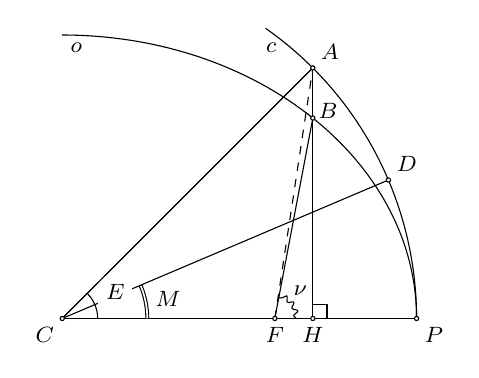
\begin{tikzpicture}[scale = 0.9]
		\footnotesize
		
		\draw (5, 0) arc(0:55:5);
		\draw (5, 0) arc(0:90:5 and 4);
		\draw (0, 0) -- (5, 0);
		
		\draw (0, 0) -- (3.536, 3.536); %%% Угол E = 45 градусов
		\draw (3, 0) -- (3.536, 2.828); %%% a * cos(45) * (b / a)
		\draw[dashed] (3, 0) -- (3.536, 3.536); %%% a * cos(45) * (b / a)
		
		\draw (0.5, 0) arc(0:45:0.5);
		\draw[double] (1.2, 0) arc(0:23:1.2);
		\draw[decoration={snake, segment length=1.1mm,
		amplitude=0.3mm}, decorate] (3.3, 0) arc(0:79.26:0.3);
		\draw (3.536, 3.536) -- (3.536, 0);
		
		\draw (0, 0) node [anchor=north east] {$C$};
		\draw (3, 0) node [anchor=north] {$F$};
		\draw (3.536, 3.536) node[anchor=south west] {$A$};
		\draw (3.5, 2.7) node[anchor=south west] {$B$};
		\draw (1.2, 0.05) node[anchor=south west] {$M$};
		\draw (0, 0) -- (4.603, 1.954); %%% a * cos(23)
		\draw (0.5, 0.15) node[anchor=south west, fill=white] {$E$};
		\draw (0, 0) -- (3.536, 3.536);
		\draw (3.15, 0.2) node[anchor=south west] {$\nu$};
		
		\draw (5, 0) node [anchor= north west] {$P$};
		\draw (3.536, 0) node [anchor= north] {$H$};
		\draw (4.603, 1.954) node [anchor=south west] {$D$};
		\draw (2.95, 4) node [anchor=north] {$c$};
		\draw (0, 4) node [anchor=north west] {$o$};
		
		\draw[fill=white] (3.536, 3.536) circle (0.03); 	 %%% A
		\draw[fill=white] (3.536, 2.828) circle (0.03); 	 %%% B
		\draw[fill=white] (0, 0) circle (0.03);			 %%% C
		\draw[fill=white] (4.603, 1.954) circle (0.03); 	 %%% D
		\draw[fill=white] (3, 0) circle (0.03); 	         %%% F
		\draw[fill=white] (3.536, 0) circle (0.03);      %%% H
		\draw[fill=white] (5, 0) circle (0.03);          %%% P
		
		\draw (3.736, 0) -- (3.736, 0.2) -- (3.536, 0.2);
		
	\end{tikzpicture}
	\caption{К выводу уравнения Кеплера}
	\label{fig:kepler-eq}
\end{wrapfigure}
Рассмотрим эллиптическую орбиту $o$ с центром в точке $C$, центральным телом в фокусе $F$ и большой полуосью $a$. Обозначим за $P$ перицентр данной орбиты, тогда $|CP| = a$. Рассмотрим также окружность $c$, с центром в точке в точке $C$ и радиусом $a$, очевидно, эта окружность будет касаться эллипса внешним образом в точке~$P$. Выберем на эллипсе произвольную точку $B$. Проведем через нее прямую, параллельную малой оси эллипса. Точку пересечения полученной прямой с окружностью $c$ назовем $A$. Угол $E = \angle ACP$ называется \term[эксцентрическая аномалия]{эксцентрической аномалией} точки $B$.


Получим связь средней аномалии $M$ с эксцентрической~--- $E$~\cite{orbital-motion-roy}. Прежде всего напомним, что эллипс является результатом действия аффинного преобразования сжатия (вдоль малой оси) на окружность с радиусом~$a$. И, наоборот, окружность под действием растяжения переходит в эллипс. В наших обозначениях будем считать, что окружность $o$ под действием сжатия $\xi$ с коэффициентом $a/b$ переходит в эллипс $o$.

\begin{figure}[h!]
	\begin{subcaptionblock}{0.47\tw}
		\begin{tikzpicture}[scale = 0.9]
			\footnotesize
			
			\draw[line width=2pt, lightgray, line join = round] (5, 0) arc(0:45:5) -- (3, 0) -- cycle;
			\draw[line width=2pt, lightgray, line join = round] (5, 0) arc(0:45:5 and 4) -- (3, 0) -- cycle;
			
			\draw [line cap = round](5, 0) arc(0:55:5);
			\draw [line cap = round] (5, 0) arc(0:90:5 and 4);
			\draw (0, 0) -- (5, 0);
			
			\draw (0, 0) -- (3.536, 3.536); %%% Угол E = 45 градусов
			\draw (3, 0) -- (3.536, 2.828); %%% a * cos(45) * (b / a)
			\draw[dashes] (3, 0) -- (3.536, 3.536); %%% a * cos(45) * (b / a)
			
			\draw (0.5, 0) arc(0:45:0.5);
			\draw[double] (1.2, 0) arc(0:23:1.2);
			\draw[decoration={snake, segment length=1.1mm, amplitude=0.3mm}, decorate] (3.3, 0) arc(0:79.26:0.3);
			\draw (3.536, 3.536) -- (3.536, 0);
			
			\draw (0, 0) node [anchor=north east] {$C$};
			\draw (3, 0) node [anchor=north] {$F$};
			\draw (3.536, 3.536) node[anchor=south west] {$A$};
			\draw (3.5, 2.7) node[anchor=south west] {$B$};
			\draw (1.2, 0.05) node[anchor=south west] {$M$};
			\draw (0, 0) -- (4.603, 1.954); %%% a * cos(23)
			\draw (0.5, 0.15) node[anchor=south west, fill=white] {$E$};
			\draw (0, 0) -- (3.536, 3.536);
			\draw (3.15, 0.2) node[anchor=south west] {$\nu$};
			
			\draw (5, 0) node [anchor= north west] {$P$};
			\draw (3.536, 0) node [anchor= north] {$H$};
			\draw (4.603, 1.954) node [anchor=south west] {$D$};
			\draw (2.95, 4) node [anchor=north] {$c$};
			\draw (0, 4) node [anchor=north west] {$o$};
			
			\draw[fill=white] (3.536, 3.536) circle (0.03); 	 %%% A
			\draw[fill=white] (3.536, 2.828) circle (0.03); 	 %%% B
			\draw[fill=white] (0, 0) circle (0.03);			 %%% C
			\draw[fill=white] (4.603, 1.954) circle (0.03); 	 %%% D
			\draw[fill=white] (3, 0) circle (0.03); 	         %%% F
			\draw[fill=white] (3.536, 0) circle (0.03);      %%% H
			\draw[fill=white] (5, 0) circle (0.03);          %%% P
			
			\draw (3.736, 0) -- (3.736, 0.2) -- (3.536, 0.2);
			
		\end{tikzpicture}
		\caption{Секторы $\sector BFP$ и $\sector AFP$}
	\end{subcaptionblock}
	\hfill
	\begin{subcaptionblock}{0.47\tw}
		\begin{tikzpicture}[scale = 0.9]
			\footnotesize
			
			\draw[line width=2pt, lightgray, line join = round] (5, 0) arc(0:23:5) -- (0, 0) -- cycle;
			\draw[line width=2pt, lightgray, line join = round] (5, 0) arc(0:45:5 and 4) -- (3, 0) -- cycle;
			
			\draw [line cap = round](5, 0) arc(0:55:5);
			\draw [line cap = round] (5, 0) arc(0:90:5 and 4);
			\draw (0, 0) -- (5, 0);
			
			\draw (0, 0) -- (3.536, 3.536); %%% Угол E = 45 градусов
			\draw (3, 0) -- (3.536, 2.828); %%% a * cos(45) * (b / a)
			\draw[dashes] (3, 0) -- (3.536, 3.536); %%% a * cos(45) * (b / a)
			
			\draw (0.5, 0) arc(0:45:0.5);
			\draw[double] (1.2, 0) arc(0:23:1.2);
			\draw[decoration={snake, segment length=1.1mm, amplitude=0.3mm}, decorate] (3.3, 0) arc(0:79.26:0.3);
			\draw (3.536, 3.536) -- (3.536, 0);
			
			\draw (0, 0) node [anchor=north east] {$C$};
			\draw (3, 0) node [anchor=north] {$F$};
			\draw (3.536, 3.536) node[anchor=south west] {$A$};
			\draw (3.5, 2.7) node[anchor=south west] {$B$};
			\draw (1.2, 0.05) node[anchor=south west] {$M$};
			\draw (0, 0) -- (4.603, 1.954); %%% a * cos(23)
			\draw (0.5, 0.15) node[anchor=south west, fill=white] {$E$};
			\draw (0, 0) -- (3.536, 3.536);
			\draw (3.15, 0.2) node[anchor=south west] {$\nu$};
			
			\draw (5, 0) node [anchor= north west] {$P$};
			\draw (3.536, 0) node [anchor= north] {$H$};
			\draw (4.603, 1.954) node [anchor=south west] {$D$};
			\draw (2.95, 4) node [anchor=north] {$c$};
			\draw (0, 4) node [anchor=north west] {$o$};
			
			\draw[fill=white] (3.536, 3.536) circle (0.03); 	 %%% A
			\draw[fill=white] (3.536, 2.828) circle (0.03); 	 %%% B
			\draw[fill=white] (0, 0) circle (0.03);			 %%% C
			\draw[fill=white] (4.603, 1.954) circle (0.03); 	 %%% D
			\draw[fill=white] (3, 0) circle (0.03); 	         %%% F
			\draw[fill=white] (3.536, 0) circle (0.03);      %%% H
			\draw[fill=white] (5, 0) circle (0.03);          %%% P
			
			\draw (3.736, 0) -- (3.736, 0.2) -- (3.536, 0.2);
			
		\end{tikzpicture}
		\caption{Секторы $\sector DCP$ и $\sector BFP$}
	\end{subcaptionblock}
	\caption{}
\end{figure}

Найдем связь площадей секторов $\sector AFP$ и $\sector BFP$. Нетрудно заметить, что первый переходит во второй под действием $\xi$. Из свойств аффинного преобразования получаем:
\begin{equation*}
	\frac{\area \sector BFP}{\area \sector AFP} = \frac{b}{a}.
\end{equation*}


Как известно, площадь эллипса $S = \pi ab$, а окружности с той же большой полуосью~---  $S' = \pi a^2$. По второму закону Кеплера радиус-вектор тела $\overrightarrow{FB}$ за равные промежутки времени заметает равные площади, то есть скорость заметания постоянна и равна $\sigma = \pi a b / T$. A из определения средней аномалии следует, что угловая скорость вектора $\overrightarrow{CD}$ также постоянна и равна $\sigma' = \pi a^2 / T$. Отсюда можно сделать вывод о следующем соотношении между площадями секторов $\sector BFP$ и $ \sector DCP$:
\begin{equation*}
	\frac{\area \sector BFP}{\area \sector DCP} = \frac{b}{a}.
\end{equation*}
Следовательно, $\area \sector DCP = \area \sector AFP$.

Как для площади центрального сектора, для $\area \sector DCP$ верно
\begin{equation*}
	\area \sector DCP = \frac{a^2}{2} M,
\end{equation*}
здесь угол $M$, конечно, в радианной мере. Аналогично для $\area \sector ACP$:
\begin{equation*}
	\area \sector ACP = \frac{a^2}{2} E.
\end{equation*}
С другой стороны $\sector ACP = \sector AFP + \triangle ACF$, а, значит,
\begin{equation}
	\area \sector ACP = \area\sector AFP + \area\triangle ACF.
	\label{eq:kepler-eq-acp}
\end{equation}
Найдем площадь треугольника $\triangle ACF$:
\begin{equation*}
	\area \triangle ACF = \frac{1}{2} |CF| \cdot |AC| \sin E = \frac{1}{2} a e \cdot a \sin E =  \frac{a^2 e\sin E}{2}
\end{equation*}
Тогда из равенства $\area \sector DCP = \area \sector AFP$ и \eqref{eq:kepler-eq-acp} получаем:
\begin{equation*}
	\frac{a^2}{2} E = \frac{a^2 e\sin E}{2} + \frac{a^2}{2} M.
\end{equation*}
Отсюда получаем так называемое \term{уравнение Кеплера}, оно связывает среднюю и эксцентрическую аномалии
\begin{equation}\label{eq:kepler-eq}
	M = E - e \sin E.
\end{equation}
Найдем теперь зависимость эксцентрической аномалии $E$ от истинной, чтобы связать все три аномалии. Вспомним, что точка $B$ принадлежит эллипсу $o$, следовательно, она удовлетворяет уравнению эллипса в декартовых координатах, значит
\begin{equation}
	\frac{|CH|^2}{a^2} + \frac{|BH|^2}{b^2} = 1.
	\label{eq:kepler-eq-dec-eq}
\end{equation}
Далее, $|CH| = |AC| \cos E = a \cos E$, как прилежащий к углу $\angle E$ катет в прямоугольном треугольнике $\triangle AHC$. Выразим теперь $|BH|$ из \eqref{eq:kepler-eq-dec-eq}:
\begin{equation*}
	|BH| = b\sqrt{1 - \frac{|CH|^2}{a^2}} = a \sqrt{1 - e^2} \sqrt{1 - \frac{a^2 \cos^2 E}{a^2}} = a \sqrt{1 - e^2} \sin E .
\end{equation*}
Найдем $|FH|$:
\begin{equation*}
	|FH| = |CH| - |CF| = a \cos E - a e = a (\cos E - e).
\end{equation*}
Запишем теорему Пифагора для прямоугольного треугольника $\triangle BHF$:
\begin{align*}
	|FB|^2 &= |FH|^2 + |BH|^2 = \\
	&= a^2 (\cos E - e)^2 + a^2 \left( 1 - e^2 \right) \sin^2 E = \\
	&= a^2 \left( \cos^2 E + e^2 - 2 e \cos E + \sin^2 E - e^2 \sin^2 E \right) = \\
	&= a^2 \Big( 1 - 2 e \cos E + e^2 \left( 1 - \sin^2 E \right) \Big) =  a^2 \left( 1 - e \cos E \right)^2
\end{align*}
Приравняем полученное выражение для $|FB|$ и выражение через уравнение эллипса в полярных координатах:
\begin{equation*}
	|FB| = r = \frac{a \left(1 - e^2 \right)}{ 1 + e \cos \nu},
\end{equation*}
\begin{equation}
	1 - e \cos E  = \frac{1 - e^2}{ 1 + e \cos \nu}.
	\label{eq:kepler-eq-E-nu-1}
\end{equation}

\newcommand{\sqTgHalf}[1]{#1'}

Приведем \eqref{eq:kepler-eq-E-nu-1} к более простому виду. Воспользуемся для этого формулой для косинуса двойного угла
\begin{equation*}
     \cos x = \frac{\raisebox{5pt}{$1 - \tg^2 \dfrac{x}{2}$}}{\raisebox{-5pt}{$1 + \tg^2 \dfrac{x}{2}$}},
\end{equation*}
подставим её в \eqref{eq:kepler-eq-E-nu-1}, приведем левую и правую части к общим знаменателям и введём обозначения $\sqTgHalf{E} \equiv \tg^2 (E/2)$ и $\sqTgHalf{\nu} \equiv \tg^2 (\nu/2)$:
\begin{gather*}
    \frac{1 + \sqTgHalf{E} - e + e \sqTgHalf{E}}{1 + \sqTgHalf{E}} = \frac{(1 - e^2) \left( 1 + \sqTgHalf{\nu} \right)}{1 + \sqTgHalf{\nu} + e - e \sqTgHalf{\nu}},\\
    \frac{(1 - e) + (1 + e) \sqTgHalf{E}}{1 + \sqTgHalf{E}} = \frac{(1-e)(1+e)\left( 1 + \sqTgHalf{\nu} \right)}{(1 + e) + (1 - e) \sqTgHalf{\nu} }.
\end{gather*}
Разделим обе части на $1 + e$, сократим правую на $1 - e$, также введём обозначение $\varepsilon = (1 - e) / (1 + e)$:
\begin{equation*}
    \frac{\varepsilon + \sqTgHalf{E}}{1 + \sqTgHalf{E}} = \frac{1 + \sqTgHalf{\nu}}{1 / \varepsilon + \sqTgHalf{\nu}}.
\end{equation*}
Перемножив члены пропорции и приведя подобные, получим
\begin{gather}
    \sqTgHalf{E} = \varepsilon \sqTgHalf{\nu},\nonumber\\
    \tg \frac{E}{2} = \sqrt{\frac{1 - e}{1 + e}} \tg \frac{\nu}{2}.
    \label{eq:kepler-eq-E-nu-2}
\end{gather}
Полученное равенство завершает систему уравнений для $\nu$, $E$ и $M$.


\subsection{Гиперболическое уравнение Кеплера}

Для гиперболы тоже есть свой вариант уравнения Кеплера. Для того, чтобы его получить запишем выражение для момента импульса и уравнение гиперболы в полярных координатах:
\begin{equation*}
    l = r^2 \dot{\nu} = \sqrt{GMp}, \quad r = \frac{p}{1 + e \cos \nu}.
\end{equation*}
Подставив одно уравнение в другое можно получить такое дифференциальное соотношение:
\begin{equation*}
    \sqrt{GMp}\,dt=\frac{p^2 \,d\nu}{(1 + e \cos{\nu})^2}.
\end{equation*}
Вспомнив значение для частоты из третьего закона Кеплера и интегрируя с обеих сторон выходит:
\begin{equation*}
    \int\limits_{\nu_1}^{\nu_2}{\frac{d\nu}{(1+e\cos \nu)^2}} = \frac{\omega T}{\sqrt{(e^2 - 1)^3}}.
\end{equation*}
Далее сделаем замену в интеграле:
\begin{equation*}
    \cos \nu = \frac{e - \cosh H}{e \cosh H - 1}, \quad \sin \nu = \frac{\sqrt{e^2-1} \sinh H}{e \cosh H - 1}.
\end{equation*}
Дифференциал тогда:
\begin{gather*}
    -\sin \nu \, d \nu = -\frac{(e^2 - 1) \sinh H}{(e \cosh H - 1)^2}\,dH = -\frac{\sqrt{e^2-1}\sin \nu}{e \cosh H - 1}\,dH, \\
    d\nu = \frac{\sqrt{e^2-1}}{e \cosh H - 1}\,dH.
\end{gather*}
После замены интеграл упрощается до:
\begin{equation*}
    \int\limits_{H_1}^{H_2}{\frac{e \cosh H - 1}{\sqrt{(e^2-1)^3}} \,dH} = \frac{\omega T}{\sqrt{(e^2 - 1)^3}}.
\end{equation*}
Отсюда получаем \term{уравнение Кеплера для гиперболы}:
\begin{equation}
    \omega T = M = e \sinh H - H.
\end{equation}

\subsection{Уравнение Баркера}
Для того, чтобы связать истинную аномалию с некоторым временем при движении тела по параболе используют \term{уравнение Баркера}.

Вспомним выражение для периода тела на орбите из третьего закона Кеплера (\ref{eq:kepler-third-law}):
\begin{equation*}
    T = 2\pi \sqrt{\frac{a^3}{GM}},
\end{equation*}
Однако с учётом того, что расстояние до перицентра  $q = a(1-e)$ и также вспомнив определение средней аномалии можно записать:
\begin{equation}
    M = t \sqrt{\frac{GM(1 - e)^3}{q^3}}.
    \label{eq:third-kepler-law-mean-anomaly}
\end{equation}
С другой стороны из уравнения Кеплера \eqref{eq:kepler-eq} и разложения синуса в ряд Тейлора~\eqref{eq:taylor-series} средняя аномалия
\begin{gather}
    M = E - e \sin E = E - e \left(E - \frac{E^3}{3!} + \frac{E^5}{5!} - \dots\right),\nonumber\\
    M = E(1-e) + e\left(\frac{E^3}{3!} - \frac{E^5}{5!} + \dots \right).
    \label{eq:kepler-eq-series}
\end{gather}
Теперь запишем формулу перехода от истинной аномалии к эксцентрической~\eqref{eq:kepler-eq-E-nu-2}:
\begin{equation*}
    \tg \frac{E}{2} = \sqrt{\frac{1-e}{1+e}} \tg \frac{\nu}{2}.
\end{equation*}
Заметим, что при всех $\nu$, исключая $\pi$, можно считать, что $E \ll 1$, так как для параболы $1-e \ll 1$. Следовательно, поскольку $\tg x \simeq x$,
\begin{equation*}
    E = 2 \sqrt{\frac{1-e}{1+e}} \tg \frac{\nu}{2}.
\end{equation*}
Подставим это в~\eqref{eq:third-kepler-law-mean-anomaly} c учётом~\eqref{eq:kepler-eq-series}:
\begin{equation*}
    M = t \sqrt{\frac{GM(1-e)^3}{q^3}} = \frac{2(1-e)^{3/2}}{\sqrt{1+e}}\tg\frac{\nu}{2} + \frac{8(1-e)^{3/2}}{3! \cdot (1+e)^{3/2}}\tg^3 \frac{\nu}{2} + \dots
\end{equation*}
Сократив на $(1-e)^{3/2}$ и приведя выражение, получим \imp{уравнение Баркера}
\begin{equation}
    t = \sqrt{\frac{2q^3}{GM}}\left(\tg \frac{\nu}{2 } + \frac{1}{3}\tg^3 \frac{\nu}{2}\right).
\end{equation}

\subsection{Точки Лагранжа}

\begin{wrapfigure}[12]{r}{0.5\tw}
	\centering
	\vspace{-1pc}
	\begin{tikzpicture}
        \def\d{3.5}
        \def\m{1}
        \def\M{3.5}
        \def\r{(3 * \M / \m)^(-1/3)}
        \def\rrr{7 * \m / (12 * \M)}
        \def\R{\fpeval{\d / (1 + 1 - \r)}}
        \def\c{\fpeval{\m / (\M + \m)}}
        \def\xL{\fpeval{\R / 2 * (\M - \m) / (\M + \m)}}
        \def\yL{\fpeval{sqrt(3) / 2 * \R}}
        
        \tkzDefPoint(0,0){M}
        \tkzDefShiftPoint[M](\R,0){m}
        \tkzDefPointBy[homothety=center M ratio \c](m) \tkzGetPoint{C}
        \tkzDefPointBy[homothety=center m ratio \r](M) \tkzGetPoint{L1}
        \tkzDefPointBy[homothety=center m ratio {-\r}](M) \tkzGetPoint{L2}
        \tkzDefPointBy[homothety=center M ratio {-1+\rrr}](m) \tkzGetPoint{L3}
        \tkzDefShiftPoint[C](\xL,\yL){L4}
        \tkzDefShiftPoint[C](\xL,-\yL){L5}
        
        \tkzDrawSegments[dashed](L2,L3 M,L4 M,L5 m,L5 m,L4)
        
        \tkzLabelPoint[below](M){\adjustbox{left=20pt}{$M_1$}}
        \tkzLabelPoint[below](m){\adjustbox{right=22pt}{$M_2$}}
        \tkzLabelPoint[above](C){ц.\,м.}
        \tkzLabelPoint[below](L1){$L_1$}
        \tkzLabelPoint[below](L2){$L_2$}
        \tkzLabelPoint[below](L3){$L_3$}
        \tkzLabelPoint[above](L4){$L_4$}
        \tkzLabelPoint[below](L5){$L_5$}
        
        \tkzMarkAngles[size=0.2](m,M,L4 M,L4,m L4,m,M)
        \tkzMarkAngles[size=0.25](L5,M,m m,L5,M M,m,L5)
        
        \tkzDrawPoints(M, m, C, L1, L2, L3, L4, L5)        
    \end{tikzpicture}
	\caption{Точки Лагранжа}
	\label{pic:larg-points}
\end{wrapfigure}
\term{Точки Лагранжа}~--- точки во вращающейся системе из двух массивных тел, в которых третье тело с пренебрежимо малой массой, не испытывающее воздействие никаких других сил, кроме гравитационных со стороны двух первых тел, может оставаться неподвижным относительно этих тел. В данных точках гравитационные силы, действующие на малое тело, уравновешиваются силами инерции.

Точки $L_1$, $L_2$ и $L_3$ лежат на одной прямой,
соединяющей два массивных тела (см.~Рис.\,\ref{pic:larg-points}).
В системе Солнце\,--\,Земля точка $L_1$ находится между Землёй и
Солнцем, $L_2$~--- с противоположной стороны от Земли, а точка
$L_3$ располагается за Солнцем. Точки $L_4$ и $L_5$
образуют равносторонние треугольники с массивными телами.

%Для расстояний до точек $L_1$, $L_2$ и $L_3$ от
%центра масс системы справедливы следующие выражения:
%\begin{equation}r_1=R\left(1-\sqrt[3]{\frac{\alpha}
%{3}}\right), \quad r_2=R\left(1+\sqrt[3]{\frac{\alpha}
%{3}}\right), \quad r_3=R\left(1+\frac{5}{12}\alpha\right),
%\end{equation}
%где $\alpha=M_2 / (M_1 + M_2)$, $R$~--- расстояние между
%телами, $M_1$ --- масса более массивного тела, $M_2$
% --- масса второго тела.
%
%Если $M_2 \ll M_1$, то точки $L_1$ и $L_2$ находятся
%примерно на одинаковом расстоянии от тела $M_2$, равном
%\begin{equation}
%r\approx R\sqrt[3]{\frac{M_2}{3M_1}}.
%\end{equation}

\begin{wrapfigure}[4]{r}{0.45\tw}
	\centering
	\vspace{-.5pc}
	\begin{tikzpicture}
        \def\R{4}
        \def\m{1}
        \def\M{5}
        \def\r{3 * \M / \m)^(-1/3)}
        \def\c{\m / (\M + \m)}
        
        \tkzDefPoint(0,0){M}
        \tkzDefShiftPoint[M](\R,0){m}
        \tkzDefPointBy[homothety=center M ratio \c](m) \tkzGetPoint{C}
        \tkzDefPointBy[homothety=center m ratio \r](M) \tkzGetPoint{L}
        
        \tkzDrawSegment[dashed](M,m)
        
        \tkzLabelPoint[above](M){$M_1$}
        \tkzLabelPoint[above](m){$M_2$}
        \tkzLabelPoint[above](C){ц.\,м.}
        \tkzLabelPoint[above](L){$L_1$}
        
        \begin{scope}[
            dim style/.style={black, latex-latex, opacity=1},
            dim fence style/.style={opacity=0}
        ]
            \tkzDrawSegment[opacity=0, dim={$R - r$, -0.2cm, below=2pt}](M,L)
            \tkzDrawSegment[opacity=0, dim={$r$, -0.2cm, below=2pt}](L,m)
        \end{scope}
        
        \tkzDrawPoints(M, m, C, L)
    \end{tikzpicture}
	\caption{Расположение точки $L_1$}
	\label{pic:larg-points-1-2}
\end{wrapfigure}Получим выражения для расстояний от центра масс системы до точек Лагранжа. Проще всего это сделать для точек $L_1$ и $L_2$. Пусть $R$~--- расстояние между телами, $M_1$ и $M_2$~--- их массы. Будем искать расстояние~$r$ до точки $L_1$ от тела $M_2$.

Из уравнения моментов сил тело с массой $M_2$ находится на расстоянии $\beta R$ от центра масс, где $\beta \equiv M_1 / (M_1 + M_2)$. Тело с массой $M_1$, соответственно, --- на расстоянии $\alpha R$, где $\alpha \equiv M_2 / (M_1 + M_2)$. Легко видеть, что $\alpha + \beta = 1$, данный факт будет использован ниже.

Запишем уравнение баланса сил, действующих на пробное тело в точке~$L_1$:
\begin{equation}
	\frac{GM_1 m}{(R - r)^2} = \frac{G M_2 m}{r^2} + m \omega^2 \left(R \cdot \frac{M_1}{M_1 + M_2} - r \right),
	\label{eq:lagrange-1}
\end{equation}
где $\omega$~--- угловая скорость вращения системы вокруг центра масс. Выразим её из обобщенного третьего закона Кеплера:
\begin{equation*}
	\frac{G \left(M_1 + M_2 \right)}{R^3} = \frac{4 \pi^2}{T^2} = \omega^2.
\end{equation*}
Подставим угловую скорость в \eqref{eq:lagrange-1}:
\begin{gather*}
	\frac{GM_1 m}{(R - r)^2} = \frac{G M_2 m}{r^2} + m \frac{G \left(M_1 + M_2 \right)}{R^3} \left(R \cdot \frac{M_1}{M_1 + M_2} - r \right),\\
	\frac{M_1}{(R - r)^2} = \frac{M_2}{r^2} + \frac{M_1 + M_2}{R^3} \left(R \cdot\frac{M_1}{M_1 + M_2} - r \right),\\
	\frac{M_1}{(R - r)^2} = \frac{M_2}{r^2} + \frac{M_1}{R^2} - \frac{\left(M_1 + M_2 \right)}{R^2} \cdot \frac{r}{R}.
\end{gather*}
Рассмотрим случай $M_2 \ll M_1$, тогда $r \ll R$, следовательно
\begin{gather*}
	\frac{M_1}{R^2} \left(1 + \frac{2r}{R} + o\left(\frac{r}{R}\right) \right) = \frac{M_2}{r^2} + \frac{M_1}{R^2} - \frac{\left(M_1 + M_2 \right)}{R^2} \cdot \frac{r}{R},\\
	\frac{M_1}{R^2} \left( 1 + \frac{2r}{R} - 1 + \frac{r}{R}  + o\left(\frac{r}{R}\right) \right) = M_2 \left( \frac{1}{r^2} - \frac{r}{R^3} \right), \\
	\frac{M_1}{R^2} \left( \frac{3r}{R} + o\left(\frac{r}{R}\right) \right) =
	% \frac{M_2}{r^2} \left( 1 - \frac{r^3}{R^3} \right) =
	\frac{M_2}{r^2} \left( 1 +  o\left(\frac{r}{R}\right)  \right),\\
	\frac{M_1}{R^2} \cdot \frac{3r}{R} \simeq \frac{M_2}{r^2} \quad \Rightarrow \quad r \simeq R \sqrt[3]{\frac{M_2}{3M_1}}.
\end{gather*}
Заметим, что уравнение для точки $L_2$ с точностью до знака перед $r$ совпадает с \eqref{eq:lagrange-1}. Следовательно, расстояние от центра масс системы до точек $L_1$ и $L_2$ определяется, как
\begin{equation}
	R_{1,2} = R \left( 1 \mp \sqrt[3]{\frac{M_2}{3M_1}} \right).
\end{equation}


\begin{wrapfigure}[4]{r}{0.4\tw}
	\centering
	\vspace{-1pc}
	\begin{tikzpicture}
        \def\d{4}
        \def\m{1}
        \def\M{2.7}
        \def\r{7 * \m / (12 * \M)}
        \def\R{\fpeval{\d / (1 + 1 - \r)}}
        \def\c{\m / (\M + \m)}
        
        \tkzDefPoint(0,0){M}
        \tkzDefShiftPoint[M](\R,0){m}
        \tkzDefPointBy[homothety=center M ratio \c](m) \tkzGetPoint{C}
        \tkzDefPointBy[homothety=center M ratio {-1+\r}](m) \tkzGetPoint{L}
        
        \tkzDrawSegment[dashed](L,m)
        
        \tkzLabelPoint[above](M){$M_1$}
        \tkzLabelPoint[above](m){$M_2$}
        \tkzLabelPoint[above](C){ц.\,м.}
        \tkzLabelPoint[above](L){$L_3$}
        
        \begin{scope}[
            dim style/.style={black, latex-latex, opacity=1},
            dim fence style/.style={opacity=0}
        ]
            \tkzDrawSegment[opacity=0, dim={$R - r$, -0.2cm, below=2pt}](L,M)
            \tkzDrawSegment[opacity=0, dim={$R$, -0.2cm, below=2pt}](M,m)
        \end{scope}
        
        \tkzDrawPoints(M, m, C, L)
    \end{tikzpicture}
	\caption{Расположение точки $L_3$}
	\label{pic:larg-points-3}
\end{wrapfigure}
Найдем теперь расстояние $R_3$ от центра масс до точки $L_3$. Пусть точка $L_3$ находится на расстоянии $R - r$ от тела с массой $M_1$. Будем искать расстояние~$r$. Запишем баланс сил, предварительно сократив на $Gm$:
\begin{equation}
	\frac{M_1}{(R - r)^2} + \frac{M_2}{(2R - r)^2} =  \frac{M_1 + M_2}{R^3} \left(R - r + R \cdot \frac{M_2}{M_1 + M_2} \right).
	\label{eq:lagrange-2}
\end{equation}
Снова рассмотрим случай $r \ll R$, когда $M_2 \ll M_1$, тогда \eqref{eq:lagrange-2} будет выглядеть, следующий образом:
\begin{gather*}
	\frac{M_1}{R^2} \left(1 + \frac{2r}{R} \right) + \frac{M_2}{4R^2} \left(1 + \frac{r}{R} \right) \simeq \frac{M_1}{R^2} + \frac{M_2}{R^2} - \frac{M_1}{R^2} \cdot \frac{r}{R} - \frac{M_2}{R^2} \cdot \frac{r}{R} + \frac{M_2}{R^2},\\
	\frac{r}{R} \left( \frac{3M_1}{R^2} + \frac{5M_2}{4R^2} \right) \simeq \frac{7M_2}{4R^2} \quad \Rightarrow \quad r \simeq R \cdot \frac{7 M_2}{12 M_1}.
	%	\frac{r}{R} \left( 3 + \frac{5M_2}{4M_1} \right) \simeq \frac{7M_2}{4M_1},\\[0.5pc]
\end{gather*}
Следовательно, расстояние до точки $L_3$ от центра масс системы равно
\begin{equation}
	R_3 \simeq R - r + R\alpha \simeq
	% 	R \left(1 - \frac{7 M_2}{12 M_1} + \frac{M_2}{M_1} \right) =
	R \left( 1 + \frac{ 5 M_2}{12 M_1} \right).
\end{equation}


Остается найти координаты точек Лагранжа $L_4$ и $L_5$, для этого рассмотрим~Рис.\,\ref{pic:larg-points-4-5_1}. Векторы $\vec{r}_1$, $\vec{r}_2$ и $\vec{r}_3$~--- радиус-векторы соответсвенно тела с массой $M_1$, тела с массой $M_2$ и центра масс относительно точки~$L_4$. В~силу симметрии  все рассуждения будут верны и для точки~$L_5$. Также на рисунке отмечены силы, действующие на тело, располагающееся в точке $L_4$: $\vec{F}_1$~--- сила гравитации от тела с массой $M_1$, $\vec{F}_2$~--- с массой $M_2$, сила инерции $\vec{F}_\text{ц.б.}$~--- центробежная, коллинеарна вектору~$\vec{r}_3$.

\begin{figure}[h!]
    \hfill
    \begin{subcaptionblock}{0.47\tw}
        \centering
		\begin{tikzpicture}
            \def\R{3.5}
            \def\m{1}
            \def\M{3}
            \def\xL{\fpeval{\R / 2 * (\M - \m) / (\M + \m)}}
            \def\yL{\fpeval{sqrt(3) / 2 * \R}}
            \def\c{\m / (\M + \m)}
        
            \tkzDefPoint(0,0){M}
            \tkzDefShiftPoint[M](\R,0){m}
            \tkzDefPointBy[homothety=center M ratio \c](m) \tkzGetPoint{C}
            \tkzDefShiftPoint[C](\xL,\yL){L}
        
            \tkzDrawSegment[dashed](M,m)
        
            \tkzLabelPoint[below](M){$M_1$}
            \tkzLabelPoint[below](m){$M_2$}
            \tkzLabelPoint[below](C){ц.\,м.}
            \tkzLabelPoint[above left=-2pt](L){$L_4$}
        
            \def\k{0.6}
            \tkzDefPointBy[homothety=center L ratio \k](M) \tkzGetPoint{F1}
            \tkzDefPointBy[homothety=center L ratio \fpeval{\k * \m / \M}](m) \tkzGetPoint{F2}
            \tkzDefPointBy[homothety=center L ratio \fpeval{-\k * (1 - \m / \M)}](C) \tkzGetPoint{Fc}
        
            \tkzDrawSegments[-latex](L,M L,C L,m)
            \tkzLabelSegment[above left=-2pt](F1,M){$\vec{r}_1$}
            \tkzLabelSegment[above right=-2pt](F2,m){$\vec{r}_2$}
            \tkzLabelSegment[right](L,C){$\vec{r}_3$}
        
            \tkzDrawSegments[thick, -latex](L,F1 L,F2 L,Fc)
            \tkzLabelSegment[left](L,F1){$\vec{F}_1$}
            \tkzLabelSegment[above right=-2pt](L,F2){$\vec{F}_2$}
            \tkzLabelSegment[below right=-2pt, pos=0.6](L,Fc){$\vec{F}_\text{ц.\,б.}$}
        
            \tkzDrawPoints(M, m, C, L)
        \end{tikzpicture}
		\caption{Основной способ поиска координат точек $L_4$ и $L_5$}
		\label{pic:larg-points-4-5_1}
	\end{subcaptionblock}
	\hfill
	\begin{subcaptionblock}{0.47\tw}
	    \centering
	    \begin{tikzpicture}
            \def\R{3.5}
            \def\m{1}
            \def\M{3}
            \def\xL{\fpeval{\R / 2 * (\M - \m) / (\M + \m)}}
            \def\yL{\fpeval{sqrt(3) / 2 * \R}}
            \def\c{\m / (\M + \m)}
        
            \tkzDefPoint(0,0){M}
            \tkzDefShiftPoint[M](\R,0){m}
            \tkzDefPointBy[homothety=center M ratio \c](m) \tkzGetPoint{C}
            \tkzDefShiftPoint[C](\xL,\yL){L}
        
            \tkzDrawSegments[dashed](M,L m,L)
        
            \tkzLabelPoint[below](M){$M_1$}
            \tkzLabelPoint[below](m){$M_2$}
            \tkzLabelPoint[below](C){ц.\,м.}
            \tkzLabelPoint[above left=-2pt](L){$L_4$}
        
            \def\k{0.6}
            \tkzDefPointBy[homothety=center L ratio \k](M) \tkzGetPoint{F1}
            \tkzDefPointBy[homothety=center L ratio \fpeval{\k * \m / \M}](m) \tkzGetPoint{F2}
            \tkzDefPointBy[homothety=center L ratio \fpeval{-\k * (1 - \m / \M)}](C) \tkzGetPoint{Fc}
        
            \tkzDrawSegments[-latex](C,M C,L C,m)
            \tkzLabelSegment[above, pos=0.4](C,M){$\vec{r}_1$}
            \tkzLabelSegment[right](C,L){$\vec{r}_2$}
            \tkzLabelSegment[above](C,m){$\vec{r}_3$}
        
            \tkzDrawSegments[thick, -latex](L,F1 L,F2 L,Fc)
            \tkzLabelSegment[left](L,F1){$\vec{F}_1$}
            \tkzLabelSegment[above right=-2pt](L,F2){$\vec{F}_2$}
            \tkzLabelSegment[below right=-2pt, pos=0.6](L,Fc){$\vec{F}_\text{ц.\,б.}$}
        
            \tkzDrawPoints(M, m, C, L)
        \end{tikzpicture}
		\caption{Альтернативный способ поиска координат точек $L_4$ и $L_5$}
		\label{pic:larg-points-4-5_2}
	\end{subcaptionblock}
	\hfill\!\!\!~
	\caption{}
\end{figure}

Будем действовать также, как с точками $L_1$, $L_2$ и $L_3$~--- запишем уравнение баланса сил, сократив на массу пробного тела $m$:
\begin{equation}
	\frac{G M_1}{\left|\vec{r}_1 \right|^3 } \vec{r}_1 + \frac{G M_2}{\left| \vec{r}_2 \right|^3} \vec{r}_2 - \omega^2 \vec{r}_3 = 0.
	\label{eq:larg-point-3}
\end{equation}


Из физического смысла радиус-вектора центра масс, что суммарная масса системы, помещенная в центр масс должна создавать такой же момент силы относительно произвольной точки, как вся система, справедливо следующее:
\begin{equation*}
	\vec{r}_3 = \frac{M_1 \vec{r}_1 + M_2 \vec{r}_2}{M_1 + M_2}.
	\label{eq:larg-point-r_3}
\end{equation*}
А так как $| \vec{r}_2 - \vec{r}_1| = R$, то выражение для силы инерции принимает вид
\begin{equation}
	\vec{F}_\text{ц.б.} = m \omega^2 \vec{r}_3 = \frac{ G m (M_1 \vec{r}_1 + M_2 \vec{r}_2)}{\left| \vec{r}_2 - \vec{r}_1 \right|^3}.
	\label{eq:larg-point-omega}
\end{equation}
Подставляя \eqref{eq:larg-point-omega} в уравнение баланса сил \eqref{eq:larg-point-3}, получим:
\begin{gather*}
	\frac{G M_1}{\left|\vec{r}_1 \right|^3 } \vec{r}_1 + \frac{G M_2}{\left| \vec{r}_2 \right|^3} \vec{r}_2 - \frac{G M_1}{\left|\vec{r}_2 - \vec{r}_1 \right|^3 } \vec{r}_1 - \frac{G M_2}{\left| \vec{r}_2 - \vec{r}_1 \right|^3} \vec{r}_2 = 0,\\
	M_1 \left(\frac{1}{\left| \vec{r}_1 \right|^3} - \frac{1}{\left|\vec{r}_2 - \vec{r}_1 \right|^3} \right) \vec{r}_1 + M_2 \left(\frac{1}{\left| \vec{r}_2 \right|^3} - \frac{1}{\left|\vec{r}_2 - \vec{r}_1 \right|^3} \right) \vec{r}_2 = 0.
\end{gather*}
В силу неколлинеарности векторов $\vec{r}_1$ и $\vec{r}_2$ получаем, что
\begin{equation}
	|\vec{r}_1| = |\vec{r}_2 - \vec{r}_1 | = |\vec{r}_2|,
\end{equation}
следовательно треугольник $\triangle M_1 L_4 M_2$ равносторонний. Значит в системе координат центра масс $y$-координата точек $L_4$ и $L_5$ равна $\pm R\sqrt{3}/2$. Найдем $x$-координату точки $L_4$ в системе координат центра масс:
\begin{equation*}
	x = -R\alpha + \frac{R}{2} = \frac{R}{2} \cdot \frac{-2 M_2 + M_1 + M_2}{M_1 + M_2} = \frac{R}{2} \cdot \frac{M_1 - M_2}{M_1 + M_2}.
\end{equation*}
Окончательно для координат точек Лагранжа в системе отсчета центра масс, с осью $x$, направленной в сторону тела с массой $M_2$, имеем следующее:
\begin{equation}
	\begin{gathered}
		\vec{r}_{1,2} = R \begin{pmatrix}
		1 \mp \sqrt[3]{\dfrac{M_2}{3M_1}}~~\\[1pc]
		0
	\end{pmatrix}; \quad
	%	\vec{r}_2 = R \begin{pmatrix}
	%		1 + \sqrt[3]{\dfrac{M_2}{3M_1}}~~\\[1pc]
	%		0
	%	\end{pmatrix}; \quad
	\vec{r}_3 = - R \begin{pmatrix}
	1 + \dfrac{ 5 M_2}{12 M_1}\\[1pc]
	0
\end{pmatrix};\\[0.5pc]
%	\vec{r}_4 = \begin{pmatrix}
%		\dfrac{R}{2} \cdot \dfrac{M_1-M_2}{M_1+M_2}\\[1pc]
%		\dfrac{\sqrt{3}R}{2}
%	\end{pmatrix}; \quad
\vec{r}_{4,5} = \begin{pmatrix}
\dfrac{R}{2} \cdot \dfrac{M_1-M_2}{M_1+M_2}\\[1pc]
\pm \dfrac{\sqrt{3}R}{2}
\end{pmatrix}.
\end{gathered}
\end{equation}


\footnotesize{Разберем также второй способ найти координаты точек $L_{4}$ и $L_5$. Рассмотрим Рис.\,\ref{pic:larg-points-4-5_2}. Пусть положение тел с массами $M_1$ и $M_2$, а также точки $L_4$, относительно центра масс задается радиус-векторами $\vec{r}_1$, $\vec{r}_2$ и $\vec{r}_3$ соответственно. Выпишем координаты этих векторов, приняв расстояние между массивными телами за $R$:
\begin{equation*}
\vec{r}_1 = \begin{pmatrix}
-R \cdot \dfrac{M_2}{M_1 + M_2}\\[.5pc]
0
\end{pmatrix} \equiv \begin{pmatrix}
-R \alpha\\
0
\end{pmatrix}; \quad
\vec{r}_2 = \begin{pmatrix}
R \cdot \dfrac{M_1}{M_1 + M_2}\\[.5pc]
0
\end{pmatrix} \equiv \begin{pmatrix}
R \beta\\
0
\end{pmatrix}; \quad
\vec{r}_3 = \begin{pmatrix}
x\\
y
\end{pmatrix}.
\end{equation*}
Координаты $(x, y)$ ненулевого вектора $\vec{r}_3$  и предстоит найти. Суть данного способа заключается в проецировании сил, действующих на пробную массу, находящуюся в точке $L_4$ на радиальную относительно центра масс ось и тангенциальную. Направление радиальной оси задается вектором $\vec{r}_3$, а тангенциальной~---  вектором ей ортогональным с координатами, например, $(y, -x)$. Обозначим его $\vec{r}_3^\perp$. Силы, принимаемые в расчет равны
\begin{gather*}
\vec{F}_1 = \dfrac{G M_1 m}{|\vec{r}_1 - \vec{r}_3 |^3} (\vec{r}_1 - \vec{r}_3) = \frac{G M_1 m}{\big[ (R \alpha + x)^2 + y^2 \big]^{3/2}}\begin{pmatrix}
-R\alpha - x\\
-y
\end{pmatrix} \equiv \frac{G M_1 m}{A}\begin{pmatrix}
-R\alpha - x\\
-y
\end{pmatrix} ,\\
\vec{F}_2 = \dfrac{G M_2 m}{|\vec{r}_2 - \vec{r}_3 |^3} (\vec{r}_2 - \vec{r}_3) = \frac{G M_2 m}{\big[ (R \beta - x)^2 + y^2 \big]^{3/2}}\begin{pmatrix}
R\beta - x\\
-y
\end{pmatrix} \equiv \frac{G M_2 m}{B}\begin{pmatrix}
R\beta - x\\
-y
\end{pmatrix},\\
\vec{F}_\text{ц.б} = m\omega^2 \vec{r}_3 = \frac{G (M_1 + M_2)m}{|\vec{r}_1 - \vec{r}_2|^3} \vec{r}_3 = \frac{G(M_1 + M_2)m}{R^3} \begin{pmatrix}
x\\
y
\end{pmatrix},
\end{gather*}
Запишем уравнение баланса этих сил в проекции на ось $\vec{r}_3^\perp$, используя координатное представление скалярного произведения:
\begin{gather*}
\frac{ \left( \vec{r_3^\perp},  \vec{F}_1 \right)}{\left| \vec{r}_3^\perp \right|} + \frac{ \left( \vec{r_3^\perp}, \vec{F}_2 \right)}{\left| \vec{r}_3^\perp \right|} = 0,\\
%		\frac{ \left( \vec{r_3^\perp} \right)_x  F_1^x + \left( \vec{r_3^\perp} \right)_y F_1^y}{ \sqrt{\left( \vec{r_3^\perp} \right)_x^2 + \left( \vec{r_3^\perp} \right)_y^2}} + \frac{ \left( \vec{r_3^\perp} \right)_x F_2^x + \left( \vec{r_3^\perp} \right)_y  F_2^y}{ \sqrt{\left( \vec{r_3^\perp} \right)_x^2 + \left( \vec{r_3^\perp} \right)_y^2}} = 0,\\
%		\frac{ y F_1^x - x F_1^y}{ \sqrt{x^2 + y^2}} + \frac{ y F_2^x - x F_2^y}{ \sqrt{x^2 + y^2}} = 0,\\
y F_1^x - x F_1^y + y F_2^x - x F_2^y = 0,\\
%		 \begin{aligned}
%		 	\frac{1}{\sqrt{x^2 + y^2}} \Bigg(&\dfrac{-y M_1 (R\alpha + x )}{\big[ (R \alpha + x)^2 + y^2 \big]^{3/2}} + \dfrac{x y M_1}{\big[ (R \alpha + x)^2 + y^2 \big]^{3/2}}  + \\
%		 	& + \frac{y M_2(R\beta - x)}{\big[ (R \beta - x)^2 + y^2 \big]^{3/2}} + \frac{xy  M_2}{\big[ (R \beta - x)^2 + y^2 \big]^{3/2}} \Bigg)= 0,
%		 \end{aligned}\\
%		 \dfrac{-y M_1 (R\alpha + x ) + x y M_1}{\underbrace{\big[ (R \alpha + x)^2 + y^2 \big]^{3/2}}_A} 	+ \frac{y M_2(R\beta - x) + xy  M_2}{\underbrace{\big[ (R \beta - x)^2 + y^2 \big]^{3/2}}_B}= 0,\\
\dfrac{-y M_1 (R\alpha + x ) + x y M_1}{A} 	+ \frac{y M_2(R\beta - x) + xy  M_2}{B}= 0,\\
%		 \dfrac{-y M_1 (R\alpha + x ) + x y M_1}{A} 	+ \frac{y M_2(R\beta - x) + xy  M_2}{B}= 0,\\
yR \left( - \frac{M_1 \alpha}{A} + \frac{M_2 \beta}{B}\right) + xy \cancelto{0}{\left( - \frac{M_1}{A} + \frac{M_1}{A} - \frac{M_2}{B} + \frac{M_2}{B} \right)} = 0.
\end{gather*}
Подставим выражения для $\alpha$ и $\beta$:
\begin{gather*}
\frac{yRM_1M_2}{M_1 + M_2} \left\{ \frac{1}{\big[ (R \alpha + x)^2 + y^2 \big]^{3/2}} - \frac{1}{\big[ (R \beta - x)^2 + y^2 \big]^{3/2}} \right\} = 0,\\
\frac{\big[ (R \beta - x)^2 + y^2 \big]^{3/2} - \big[ (R \alpha + x)^2 + y^2 \big]^{3/2}}{\big[ (R \alpha + x)^2 + y^2 \big]^{3/2}\big[ (R \beta - x)^2 + y^2 \big]^{3/2}} = 0.
%		 \big[ (R \beta - x)^2 + y^2 \big]^{3/2} = \big[ (R \alpha + x)^2 + y^2 \big]^{3/2},\\
\end{gather*}
Заметим, полученное уравнение верно лишь при равенстве нулю числителя, что равносильно условию $R \beta - x = R \alpha + x$, следовательно,
\begin{equation*}
	 x = \frac{R}{2} \left( \beta - \alpha \right) = \frac{R}{2} \cdot \frac{M_1 - M_2}{M_1 + M_2}.
\end{equation*}
Важно отметить, при полученном значении $x$ выполняется равенство $A = B$, чем мы сейчас и воспользуемся. Найдём возможные значения $y$, при заданном значении $x$, полученном выше. Для этого запишем уравнения баланса сил  $\vec{F}_1$, $\vec{F}_2$ и $\vec{F}_\text{ц.б}$ на ось $\vec{r_3}$:
\begin{gather*}
\frac{ \left( \vec{r_3},  \vec{F}_1 \right)}{\left| \vec{r}_3 \right|} + \frac{ \left( \vec{r_3}, \vec{F}_2 \right)}{\left| \vec{r}_3\right|} + \frac{m \omega^2 \left(\vec{r}_3, \vec{r}_3\right)}{\left| \vec{r}_3\right|} = 0,\\
\frac{-x M_1 (R \alpha + x) - y^2 M_1}{A} + \frac{ x M_2 ( R \beta - x) - y^2 M_2}{B} + \frac{M_1 + M_2}{R^3} \cdot \left( x^2 + y^2 \right) = 0,\\
\left( x^2 + y^2 \right) \left(   - \frac{M_1}{A} - \frac{M_2}{B} + \frac{M_1 + M_2}{R^3}\right) + xR \cancelto{0}{\left(  - \frac{M_1 \alpha}{A} + \frac{M_2 \beta}{B} \right)} = 0,\\
%		\left( x^2 + y^2 \right) \left(  \frac{M_1 + M_2}{R^3} - \frac{M_1 + M_2}{B} \right) + \cancelto{0}{\frac{xR M_1 M_2}{M_1 + M_2} \left( \frac{1}{B} - \frac{1}{B} \right)} = 0,\\
\left( x^2 + y^2 \right)(M_1 + M_2) \left(  - \frac{1}{B} + \frac{1}{R^3} \right) = 0.
%		B = R^3,\\
%		y^2 = R^2 \left( 1 - \left(\frac{1}{2}\left(\beta - \alpha \right) - \beta \right)^2\right) = R^2 \left( 1 - \frac{1}{4}(\underbrace{\beta + \alpha}_{1})^2 \right) = \frac{3}{4}R^2,\\
\end{gather*}
Случай $x = y = 0$ нарушает предположение $\vec{r}_3 \not = \vec{0}$, значит приведенное выше равенство выполняется только при условии $R^3 = B$, иначе,
\begin{equation*}
	(x - R \beta)^2 + y^2 = R^2 \quad \Rightarrow y = \pm \frac{\sqrt{3}}{2} R.
\end{equation*}
Полученные координаты совпадают с найдеными ранее. Относятся, соответственно, к точкам $L_4$ и $L_5$.
}
}
\subsection{Сфера действия, сфера Хилла}
\term{Сфера действия}~--- область пространства внутри которой возмущение от внешнего тела относительно планеты меньше, чем возмущение от планеты относительно внешнего тела. То есть лёгкое отклонение от положения на орбите не должно приводить к уводу внешним телом. В первом приближении данная область~--- сфера. Приведем  классический вывод её радиуса:

Для этого рассмотрим две точечные массы~$A$ и $B$ расположенные в точках $\vec{r}_A$ и $\vec{r}_B$, с массами $M_A$ и $M_B$ соответственно. Расстояние между объектами $R=\left|r_B-r_A\right|$. Введем третью безмассовую частицу $C$ в точке $\vec{r}_{\text{C}}$. Далее для анализа динамики движения точки $C$ мы можем рассматривать задачу как в системе отсчета точки $A$, так и точки $B$.

Рассмотрим систему отсчета связанную с точкой~$A$. Точка~$B$ с силой гравитации которую мы обозначим как~$g_B$ будет возмущать точку~$C$ относительно гравитации~$g_A$ точки~$A$. Вследствие закона всемирного тяготения, точка~$A$ будет притягиваться к точке~$B$ с ускорением 
\begin{equation*}
    \vec{a}_A=\frac{G M_B}{R^3}\left(\vec{r}_B-\vec{r}_A\right),
\end{equation*}
а значит данная система отсчета неинерциальна. Для того чтобы оценить эффекты возмущений в данной системе отсчета можно рассмотреть отношение величины данных возмущений к основному гравитирующему телу, то есть:
\begin{equation*}
    \chi_A=\frac{\left|g_B-a_A\right|}{\left|g_A\right|}.
\end{equation*}
Возмущающая сила $g_B-a_A$ также известна как приливная (\ref{Ebb_flow}). Аналогичным образом строится $\chi_B$ для системы отсчета точки $B$, в выводе требуется лишь провести замену $A \leftrightarrow B$.

По приближении точки $C$ к $A, \chi_A \rightarrow 0$ и $\chi_B \rightarrow \infty$, и в обратную сторону. Главным считается тот объект относительно которого отношение возмущающих сил меньше, чем относительно другого. Поверхность для которой $\chi_A=\chi_B$ разграничивает пространство на области влияния того или иного тела. В общем случае эта поверхность имеет сложную форму, однако в случае когда масса одного тела много больше другого, скажем $M_A \ll M_B$, возможно найти хорошую аппроксимацию этой разграничивающей поверхности. В этом случае поверхность будет располагаться вокруг точки~$A$, обозначим $r$ расстояние от точки $A$ до разграничивающей поверхности.

Главное ускорение в системе отсчета точки $A$ будет равно $g_A$:
\begin{equation*}
    g_A = \frac{GM_A}{r^2}.
\end{equation*}
Ускорение системы отсчета $a_A$ по модулю равно:
\begin{equation*}
    a_A = \frac{GM_B}{R^2}.
\end{equation*}
Вторичное же ускорение равно:
\begin{equation*}
    g_B\simeq\frac{GM_B}{R^2}+\frac{GM_B}{R^3}r.
\end{equation*}
Приливные силы тогда как разность вторичного ускорения и ускорения системы отсчёта:
\begin{equation*}
    g_B-a_A \simeq \frac{G M_B}{R^3} r.
\end{equation*} 
Заключая находим отношение $\chi_A$:
\begin{equation*}
    \chi_A\simeq\frac{M_B}{M_A} \frac{r^3}{R^3}.
\end{equation*}
Аналогично для системы отсчёта точки $B$. Главным ускорением тут будет $g_B$, а вторичным $g_A$. Вследстивие массивности тела $B$ ($M_A~\ll~M_B$) ускорение системы отсчета можно принять равным 0:
\begin{equation*}
    a_B=\frac{G M_A}{R^2} \simeq 0,
\end{equation*}
тогда приливные силы равные $g_A-a_B$ будут численно равны $g_A$. Отсюда отношение $\chi_B$ равно:
\begin{equation*}
    \chi_B \simeq \frac{M_A}{M_B} \frac{R^2}{r^2}.
\end{equation*}
Расстояние до сферы действия должно удволетворять равенству:
\begin{equation*}
    \frac{M_B}{M_A} \frac{r^3}{R^3}=\frac{M_A}{M_B} \frac{R^2}{r^2},
\end{equation*}
а отсюда мы можем записать выражение для радиуса сферы действия точки $A$:
\begin{equation}
    \frac{r}{R}=\left(\frac{M_A}{M_B}\right)^{2 / 5}.
\end{equation} 
\term{Сфера Хилла}~--- одна из моделей рассчета радиуса \imp{сферы действия}. Имеет физический смысл области пространства вокруг некоторого объекта (планеты) в которой его собственное гравитационное влияние на пробную массу больше, чем от внешних тел (Солнца). В первом приближении данная область~--- сфера, содержащая на себе точку $L_1$ \eqref{eq:lagrange-12} интересующей системы. В обозначениях предыдущей задачи её радиус будет выражаться как:
\begin{equation}
    \frac{r}{R} = \sqrt[3]{\frac{M_A}{3M_B}}.
\end{equation}
\begin{wrapfigure}[13]{r}{0.4\tw}
    \centering
    \vspace{-1pc}
    \tikzsetnextfilename{hill-influence-sphere-plot}
    \begin{tikzpicture}
        \begin{axis}[
            width   =   5cm,
            height  =   5cm,
            xlabel  =   {$\lg(M_B / M_A)$},
            ylabel  =   {$r/R$},
            ymax    =   0.3,
            ymin    =   0,
            xmax    =   5,
            xmin    =   1.5,
            legend cell align=left,
            legend style={
                row sep =   0.8pc,
                draw    =   none,
                fill    =   none,
                font    =   \scriptsize,
                at      =   {(axis cs:2, 0.285)}, anchor=north west,
            },
        ]
            \addplot [domain=1.5:5, samples=100, black] {10 ^ (-2 * x / 5)};
            \addplot [domain=1.5:5, samples=100, dash pattern=on 6pt off 2pt on 1pt off 2pt] {1 / (3 * 10^x)^(1/3)};

            \legend{
                Сфера действия,
                Сфера Хилла
            }
        \end{axis}
    \end{tikzpicture}
    \caption{Сравнение радиусов сферы действия и сферы Хилла}
    \label{pic:hill-influence-sphere-plot}
\end{wrapfigure} 
Часто про сферу Хилла можно услышать что она является областью пространства в которой объект может иметь собственный спутник, однако в реальности же на расстоянии равной сфере Хилла любое внешнее возмущение будет уводить спутник с орбиты и по-настоящему стабильные обриты имеют радиусы в 2-3 раза меньшие, чем сфера Хилла.
 График сравнения радиусов сферы действия и сферы Хилла для разных отношений масс $M_A$ и $M_B$ приведен правее. При отношении масс тел порядка 250 размеры сфер сравнимы между собой, однако же для малых тел для которых параметр $\lg(M_{\astrosun} / M)>6$ сфера действия будет уже вдвое меньше сферы Хилла. 
\begin{figure}[h!]
\tikzsetnextfilename{hill-influence-sphere-bar-plot2}
\begin{tikzpicture}
\begin{axis}[
    ybar,
    ymode=log,
    enlargelimits=0.15,
    legend cell align=left,
    legend style={at={(0.03,0.97)},
                    row sep = 0.8pc,
                    font=\scriptsize,
                    anchor=north west,
                    draw=none,},
    ylabel={млн. км},
    symbolic x coords={Меркурий,Венера,Земля,Марс,Юпитер,Сатурн,Уран,Нептун},
    xtick=data,
    width    =    \tw,
    height    =    6cm,
    ]
\addplot[pattern=dots] coordinates {(Меркурий,0.117) (Венера, 0.616) (Земля, 0.929) (Марс, 0.578) (Юпитер, 48.2) (Сатурн, 54.5) (Уран, 51.9) (Нептун, 86.2)};
\addplot[pattern=grid] coordinates {(Меркурий, 0.1753) (Венера, 1.0042) (Земля, 1.4714) (Марс, 0.9827) (Юпитер, 50.5736) (Сатурн, 61.6340) (Уран, 66.7831) (Нептун, 115.0307)};
\legend{Cфера действия,
        Сфера хилла}
\end{axis}
\end{tikzpicture}
\caption{Радиусы сферы действия и сферы Хилла для разных планет}
    \label{pic:hill-influence-sphere-bar-plot2}
\end{figure}

\subsection{Гравитационный манёвр}
\label{sec:grav-assist}

\term{Гравитационный манёвр}~--- изменение направления и скорости движения космического аппарата, а как следствие и параметров орбиты, в результате гравитационного взаимодействия с массивным третьим телом. Может осуществляться с применением тяги двигателя и без.

В общем случае рассматривается незамкнутое движение аппарата вокруг третьего тела, иначе  аппарат становится его спутником. Рассмотрим гравитационный маневр без двигателя подробнее и найдем максимальное достижимое в этом случае изменение скорости.

\begin{wrapfigure}[16]{r}{0.55\tw}
    \centering
    \vspace{-0.5pc}
    \begin{tikzpicture}        
        \pgfmathsetmacro\r{3}
        \pgfmathsetmacro\a{1}
        \pgfmathsetmacro\b{1.5}
        \pgfmathsetmacro\c{sqrt(\a^2 + \b^2}
        \pgfmathsetmacro\al{acos(\a / \c)}
        \pgfmathsetmacro\f{-\al}
        \pgfmathsetmacro\dx{\c * cos(\al)}
        \pgfmathsetmacro\dy{-\b}
        \pgfmathsetmacro\t{(sin(\f) - \b * \a * cos(\f)) / (cos(\f) + \b / \a * sin(\f))}
        \pgfmathsetmacro\d{-(\dy)^2 + \r^2 + 2 * \dx * \dy * \t - (\dx)^2 * \t^2 + \r^2 * \t^2}
        

        \tkzDefPoint(0,0){O}
        \tkzDefPoint(0,\r){Y}
        
        
        \tkzDrawCircle[dotted, black, line width=0.4pt](O,Y)
        
        \pgfmathsetmacro\xI{sqrt(\r^2-(\dy)^2)}
        \tkzDefShiftPoint[O](\xI,-\dy){I}
        \tkzDefPointBy[reflection = over O--Y](I) \tkzGetPoint{I'}
        
        \tkzDrawSegment[dashed](I,I')
        

        \pgfmathsetmacro\xJ{(\dy * \t - \dx * \t^2 + sqrt(\d))/(1 + \t^2)}
        \pgfmathsetmacro\yJ{sqrt(\r^2 - (\xJ)^2)}
        \tkzDefPoint(\xJ,\yJ){J}
        
        \pgfmathsetmacro\xJ{(\dy * \t - \dx * \t^2 - sqrt(\d))/(1 + \t^2)}
        \pgfmathsetmacro\yJ{-sqrt(\r^2 - (\xJ)^2)}
        \tkzDefPoint(\xJ,\yJ){J'}

        \tkzDrawSegment[dashed](J,J')
        
        
        \pgfmathsetmacro\nn{acos((\a * \r - \b^2) / \c / \r)}
        \pgfmathsetmacro\nBegin{\f + \nn}
        \pgfmathsetmacro\nEnd{360 + \f - \nn}
        
        \newcommand{\defHypPoint}[2]{
            \pgfmathsetmacro\rr{\b^2 / \a / (1 - \c / \a * cos(#1 - \f))}
            \tkzDefPoint({\rr * cos(#1 / 180 * pi)}, {\rr * sin(#1 / 180 * pi)}){#2}
        }
        \defHypPoint{\nBegin}{H'}
        \foreach \n in {\fpeval{\nBegin},\fpeval{\nBegin + 3},...,\fpeval{\nEnd},\fpeval{\nEnd}} {
            \defHypPoint{\n}{H}
            \tkzDrawSegment[line width=0.6pt](H',H)
            \tkzDefShiftPoint[H](0,0){H'}
        }
        

        \tkzDefPoint({\r * cos(\nBegin / 180 * pi)},{\r * sin(\nBegin / 180 * pi)}){B}
        \tkzDefPoint({\r * cos(\nEnd / 180 * pi)},{\r * sin(\nEnd / 180 * pi)}){E}
        

        \tkzDefPointBy[projection = onto I--I'](O) \tkzGetPoint{P}
        \tkzInterLL(I,I')(J,J') \tkzGetPoint{C}
        \tkzDefPointBy[homothety=center O ratio {1 - \a/\c}](C) \tkzGetPoint{Q}
        

        \def\vPx{-0.6}
        \def\vPy{0.4} 
        \tkzDefShiftPoint[O](\vPx,\vPy){O'}
        \tkzDefPointWith[orthogonal,K=-1.25](Q,O) \tkzGetPoint{Q'}
        

        \def\vRIx{-0.7}
        \def\vRIy{-0.043}
        \tkzDefShiftPoint[B](\vRIx,\vRIy){Vri}
        \tkzDefShiftPoint[B]({\vPx + \vRIx},{\vPy + \vRIy}){Vi}
        \tkzDefShiftPoint[B](\vPx,\vPy){Pi}
        
        \tkzLabelSegment[above,pos=0.7](B,Vi){$\vec{v}_0$}
        \tkzLabelSegment[below=-1pt, pos=0.4](B,Vri){$\vec{v}_0'$}
        \tkzLabelSegment[above right=-2pt, pos=0.7](B,Pi){$\vec{u}$}
        
        
        \def\vROx{-0.3}
        \def\vROy{-0.6}
        \tkzDefShiftPoint[E](\vROx,\vROy){Vro}
        \tkzDefShiftPoint[E](\vPx,\vPy){Eo}
        \tkzDefShiftPoint[E]({\vPx + \vROx},{\vPy + \vROy}){Vo}
        
        
        \tkzLabelSegment[above=-1pt, pos=0.6](E,Vo){$\vec{v}_1$}
        \tkzLabelSegment[right, pos=0.6](E,Vro){$\vec{v}_1'$}
        \tkzLabelSegment[above right=-2pt, pos=0.6](E,Eo){$\vec{u}$}
        
        
        \tkzLabelSegment[below left=-2pt](O,O'){$\vec{u}$}
        \tkzLabelSegment[above left=-3pt](Q,Q'){$\vec{v}_\text{макс}$}
        
        
        \tkzLabelSegment[right=-1pt](O,P){$b$}
        \tkzLabelSegment[above right=-4pt](O,Q){$q$}
        
        \tkzMarkRightAngle[size=0.15](Q',Q,O)
        \tkzMarkRightAngle[size=0.15](O,P,I)
        
        \tkzDefPointBy[homothety=center O ratio {-\c/\a}](Q) \tkzGetPoint{X}
        
        \tkzDefShiftPoint[X](\vROx,\vROy){VroX}
        \tkzDefShiftPoint[X](\vRIx,\vRIy){VriX}
        \tkzDefShiftPoint[X]({\vROx - \vRIx},{\vROy - \vRIy}){dV}
        
        \tkzLabelSegment[above](X,VriX){$\vec{v}_0'$}
        \tkzLabelSegment[left, pos=0.6](X,VroX){$\vec{v}_1'$}
        \tkzLabelSegment[above right=-2pt, pos=0.6](X,dV){$\Delta\vec{v}$}
        
        \tkzDrawSegments[line width=1pt, -latex](B,Vri B,Vi B,Pi E,Vro E,Vo E,Eo O,O' Q,Q' X,VriX X,dV X,VroX)
        
        
        \tkzMarkAngle[size=0.5](I',C,J')
        \tkzLabelAngle[pos=0.7](I',C,J'){\footnotesize$\varphi$}
        
        \tkzDrawSegments(O,P O,Q)
        
        \tkzDrawPoints(O, B, E, Q)
    \end{tikzpicture}
    \caption{Схема гравитационного маневра}
    \label{pic:grav-assist}    
\end{wrapfigure}
Пусть третье тело и аппарат в момент входа второго в область гравитационного влияния первого имеют гелиоцентрические скорости $\vec{u}$ и $\vec{v}_0$ соответственно. Тогда скорость аппарата относительно третьего тела в момент входа в область его гравитационного влияния $\vec{v}_0' = \vec{v}_0 - \vec{u}$. Обозначим $|\vec{v}_0'| \equiv v_\infty$.

Из закона сохранения энергии ясно, что максимальная скорость $\vec{v}_\text{макс}$ достигается на минимальном расстоянии $q$ от гравитирующего тела, а из минимальности расстояния следует перпендикулярность вектора скорости к радиус-вектору аппарата в этот момент. Исходя из этого, запишем законы сохранения для момента пересечения сферы влияния тела и момента максимального сближения с ним:
\begin{align*}
    \text{ЗСМИ:}&\quad v_\infty b = q v_\text{макс},\\
    \text{ЗСЭ:}&\quad \frac{v_\infty^2}{2} = \frac{v_\text{макс}^2}{2} - \frac{GM}{q}.
\end{align*}
Откуда можно выразить максимальную скорость:
\begin{equation*}
    v_\text{макс} = \sqrt{v_\infty^2 + \frac{2GM}{q}} = \sqrt{v_\infty^2 + \frac{2 v_1^2}{ \rho}},\\ \quad \rho \equiv \frac{q}{R_\text{пл}} > 1,
\end{equation*}
где $v_1$~--- первая космическая скорость на поверхности тела. Далее, прицельный параметр гиперболической орбиты аппарата $b = \sqrt{e^2 - 1}$, с другой стороны
\begin{equation*}
     b = q \frac{v_\text{макс}}{v_\infty} = a(e - 1)\sqrt{1 + \frac{2 v_1^2}{\rho v_\infty^2}} = a\sqrt{e^2 - 1}.
\end{equation*}
Получаем уравнение на эксцентриситет:
\begin{gather*}
    \sqrt{\frac{e + 1}{e - 1}} 
        = \sqrt{1 + \frac{2 v_1^2 }{ \rho v_\infty^2}}
        = \sqrt{1 + \frac{2 }{\rho\nu^2}}, 
        \quad \nu \equiv \frac{v_\infty}{v_1} > 0;\\
    e(\rho, \nu) = \rho\nu^2 + 1.
\end{gather*}

Далее находим зависимость угла поворота, что то же самое, угла между асимптотами орбиты, от входных параметров:
\begin{gather*}
    \alpha = 2 \arctg \frac{b}{a} = 2 \arctg \frac{a \sqrt{e^2 - 1}}{a} = 2 \arctg \sqrt{e^2 - 1},\\
    \alpha(\rho, \nu) = 2 \arctg \sqrt{(\rho\nu^2 + 1)^2 - 1},\\
    \varphi(\rho, \nu) = \pi - \alpha( \rho, \nu).
\end{gather*}

В силу симметрии гиперболы и законов сохранения величина относительной скорости в момент выхода из области гравитационного влияния третьего тела $|\vec{v}_1'| = v_\infty$. Остается с помощью теоремы косинусов определить $\Delta v$~--- величину приращения скорости, получаемого при гравитационном манёвре, 
\begin{gather*}
    (\Delta v)^2 = 2 v_\infty^2 - 2 v_\infty^2 \cos \varphi = 2 v_\infty^2(1 + \cos \alpha),\\
    \frac{\Delta v}{v_1} = \nu \sqrt{2 \left[ 1 + \cos \left(2 \arctg \sqrt{(\rho\nu^2 + 1)^2 - 1} \right) \right]}. 
\end{gather*}

Для нахождения максимального приращения скорости необходимо решить задачу оптимизации, решение которой выходит за рамки этой книги, поэтому сразу приведем ответ:
\begin{equation*}
    (\rho_0, \nu_0)
        = \underset{\rho \geqslant 1,~\nu \geqslant 0} \argmax\, \frac{\Delta v (\rho, \nu)}{v_1} 
        = (1, 1).
\end{equation*}
Следовательно, максимальное приращение скорости при гравитационном маневре с выключенным двигателем составляет
\begin{equation*}
    (\Delta v)_\text{макс}
        = \Delta v (\rho_0, \nu_0)
%        = \nu_0 v_1 \sqrt{2 \left[ 1 + \cos \left(2 \arctg \sqrt{(\rho_0\nu_0^2 + 1)^2 - 1} \right) \right]}
        = \sqrt{\frac{G M}{R}}.
\end{equation*}

\begin{wrapfigure}[11]{r}{0.45\tw}
    \vspace{-1.2pc}
    \begin{tikzpicture}
		\begin{axis} [
			width    = 4cm,
			height   = 4cm,
			colormap = {GS}{rgb(0cm)=(0.3, 0.3, 0.3) rgb(1cm)=(1, 1, 1)},
			xlabel 	 = {$\rho$},
			ylabel 	 = {$\nu$},
			zlabel 	 = {$I/I_0$},
			view	 = {0}{90},
			ytick    = {0,1,2,3,4},
			xtick	 = {1,2,3,4,5},
			colorbar,
			colorbar style = {ytick = {0, .2, .4, .6, .8, 1.}}
		]
				
			\addplot3[surf,shader=interp] table[x=r, y=v, z=D] {data/grav-assist.txt};
		\end{axis}
	\end{tikzpicture}
	\caption{Зависимость величины приращения скорости $\frac{\Delta v}{v_1}$ от параметров $\rho$ и $\nu$}
\end{wrapfigure}
Важно понимать, полученная величина достигается только при определенной скорости входа в зону гравитационного влияния тела, а также при сверхблизком по меркам современной космонавтики пролёте. Поэтому в действительности гравитационные маневры добавляют лишь некоторую часть этой скорости, которая используется для ускорения, торможения или поворота.

Отличительной особенность гравитационного манёвра с включением двигателя является возможное различие величины скорости входа и выхода из зоны влияния тела. Тем самым можно достичь произвольного изменения скорости, если это позволяют запасы топлива на борту аппарата.


\subsection{Годограф}
\begin{wrapfigure}[10]{r}{0.4\tw}
    \centering
    \vspace{-1.2pc}
    \tikzsetnextfilename{hodograph1}
    \begin{tikzpicture}
        \footnotesize
        \def\r{1.8}
        \def\bByA{0.7}
        
        \def\c{\r * sqrt(1 - \bByA^2)}
        \tkzDefPoint(0,0){O};
        \tkzDefPoint(\c,0){F};

        \begin{scope}[yscale=\bByA]
            \tkzDefPoint(0:\r){A_1};
            \tkzDefPoint(12.5:\r){A_2};
            \tkzDefPoint(26.5:\r){A_3};
            \tkzDefPoint(44.4:\r){A_4};
            \tkzDefPoint(70.6:\r){A_5};
            \tkzDefPoint(113.5:\r){A_6};
            \tkzDefPoint(180:\r){A_7};
            \tkzDefPoint(-113.5:\r){A_8};
            \tkzDefPoint(-70.6:\r){A_9};
            \tkzDefPoint(-44.4:\r){A_10};
            \tkzDefPoint(-26.5:\r){A_11};
            \tkzDefPoint(-12.5:\r){A_12};


            \tkzDefLine[perpendicular=through A_1](O,A_1)\tkzGetPoint{A_1'}
            \tkzDefBarycentricPoint(A_1=1,A_1'=2.5)\tkzGetPoint{1}
            \tkzDefLine[perpendicular=through A_2](O,A_2)\tkzGetPoint{A_2'}
            \tkzDefBarycentricPoint(A_2=1,A_2'=2.2)\tkzGetPoint{2}
            \tkzDefLine[perpendicular=through A_3](O,A_3)\tkzGetPoint{A_3'}
            \tkzDefBarycentricPoint(A_3=1,A_3'=1.9)\tkzGetPoint{3}
            \tkzDefLine[perpendicular=through A_4](O,A_4)\tkzGetPoint{A_4'}
            \tkzDefBarycentricPoint(A_4=1,A_4'=1.6)\tkzGetPoint{4}
            \tkzDefLine[perpendicular=through A_5](O,A_5)\tkzGetPoint{A_5'}
            \tkzDefBarycentricPoint(A_5=1,A_5'=1.3)\tkzGetPoint{5}
            \tkzDefLine[perpendicular=through A_6](O,A_6)\tkzGetPoint{A_6'}
            \tkzDefBarycentricPoint(A_6=1,A_6'=1)\tkzGetPoint{6}
            \tkzDefLine[perpendicular=through A_7](O,A_7)\tkzGetPoint{A_7'}
            \tkzDefBarycentricPoint(A_7=1,A_7'=0.7)\tkzGetPoint{7}
            \tkzDefLine[perpendicular=through A_12](O,A_12)\tkzGetPoint{A_12'}
            \tkzDefBarycentricPoint(A_12=1,A_12'=2.2)\tkzGetPoint{12}
            \tkzDefLine[perpendicular=through A_11](O,A_11)\tkzGetPoint{A_11'}
            \tkzDefBarycentricPoint(A_11=1,A_11'=1.9)\tkzGetPoint{11}
            \tkzDefLine[perpendicular=through A_10](O,A_10)\tkzGetPoint{A_10'}
            \tkzDefBarycentricPoint(A_10=1,A_10'=1.6)\tkzGetPoint{10}
            \tkzDefLine[perpendicular=through A_9](O,A_9)\tkzGetPoint{A_9'}
            \tkzDefBarycentricPoint(A_9=1,A_9'=1.3)\tkzGetPoint{9}
            \tkzDefLine[perpendicular=through A_8](O,A_8)\tkzGetPoint{A_8'}
            \tkzDefBarycentricPoint(A_8=1,A_8'=1)\tkzGetPoint{8}

            \tkzDrawSegments[-latex](A_1,1 A_2,2 A_3,3 A_4,4 A_5,5 A_6,6 A_7,7 A_8,8 A_9,9 A_10,10 A_11,11 A_12,12)
            \tkzDrawSegments(F,A_1 F,A_2 F,A_3 F,A_4 F,A_5 F,A_6 F,A_8 F,A_9 F,A_10 F,A_11 F,A_12)

            \tkzLabelPoints[above](2,3,4,5,6);
            \tkzLabelPoints[below](7,8,9);
            \tkzLabelPoints[above right](1,12);
            \tkzLabelPoints[below right](11,10);

            \draw [line width=.4pt] (F) -- (A_7) node[midway,above]{$R$};

            \draw [fill=lightgray] (F) -- (A_1) arc(0:12.5:1.8) -- cycle;
            \draw [fill=lightgray] (F) -- (A_7) arc(180:246.5:1.8) -- cycle;

            \tkzMarkAngles[size=0.3](A_1,F,A_2 A_7,F,A_8)
           
            \draw[thick] (O) circle (\r cm);
        \end{scope}
        \sun(F)
    \end{tikzpicture}
    \caption{Разбиение на секторы}
    \label{pic:hodograph1}
\end{wrapfigure}
Рассмотрим разбиение эллипса на секторы равной инстинной аномалии. Можно заметить, что из второго закона Кеплера время прохождения одного сектора пропорционально квадрату расстояния до фокуса, обозначим это время за $\Delta t$:
\begin{equation*}
    \Delta t \sim S \sim R^2.
\end{equation*}
Также из второго закона Ньютона известно соотношение:
\begin{equation*}
    \frac{\Delta v}{\Delta t} \sim R^{-2}.
\end{equation*}
Отсюда можем заключить, что:
\begin{equation*}
    \Delta v \sim \Delta t \cdot R^{-2} \sim  R^2 \cdot R^{-2} \sim \text{const}.
\end{equation*}
Значит при прохождении каждого сектора вектор скорости изменяется на некоторую постоянную величину, а также из-за того, что векторы силы и, соответственно, ускорения всегда направлены в сторону Солнца, при прохождении каждого сектора вектор скорости поворачивается на постоянный угол.

\begin{wrapfigure}[10]{l}{0.33\tw}
    \centering
    \vspace{-1pc}
    \tikzsetnextfilename{hodograph2}
    \begin{tikzpicture}
        \footnotesize
        \def\r{1.5}
        \def\bByA{0.7}

        \def\c{\r * sqrt(1 - \bByA^2)}
        \tkzDefPoint(0,0){O};
        \tkzDefPoint(0,-\c){F};
        \tkzDefPoint(0:\r){10};
        \tkzDefPoint(30:\r){11};
        \tkzDefPoint(60:\r){12};
        \tkzDefPoint(90:\r){1};
        \tkzDefPoint(120:\r){2};
        \tkzDefPoint(150:\r){3};
        \tkzDefPoint(180:\r){4};
        \tkzDefPoint(210:\r){5};
        \tkzDefPoint(240:\r){6};
        \tkzDefPoint(270:\r){7};
        \tkzDefPoint(300:\r){8};
        \tkzDefPoint(330:\r){9};

        \tkzDrawSegments[line width=.4pt,-latex](F,1 F,2 F,3 F,4 F,5 F,6 F,7 F,8 F,9 F,10 F,11 12,1 1,2 2,3 3,4 4,5 5,6 6,7 7,8 9,10 10,11 11,12)
        \draw [line width=.4pt,-latex] (F) -- (12) node[pos=0.7, right]{$v$};
        \draw [line width=.4pt,-latex] (8) -- (9) node[midway,below right]{$\Delta v$};

        \draw [line width=.4pt] (O) -- (3);

        \tkzMarkAngle[size=0.4](1,O,3)
        \tkzLabelAngle[pos=0.6](1,O,3){\footnotesize$\nu$}

        \tkzDrawPoints(1,2,3,4,5,6,7,8,9,10,11,12,O,F);
        \tkzLabelPoints[above](1,2,12);
        \tkzLabelPoints[left](3,4,5);
        \tkzLabelPoints[below](6,7,8);
        \tkzLabelPoints[right](9,10,11);
    \end{tikzpicture}
    \caption{Годограф}
    \label{pic:hodograph2}
\end{wrapfigure}
\noindent Геометрически это означает, что вектор скорости будет описывать многоугольник у которого все стороны равны, а также между собой равны все внешние углы, значит этот многоугольник правильный. При устремлении количества секторов на бесконечность фигура будет сходиться к \imp{окружности}. Годограф позволяет решать задачи в пространстве скоростей. Из факта центральности силы гравитации следует, что центральный угол на годографе напрямую соотносится с истинной аномалией, а также нетрудно показать, что при единичной нормировке размера годографа, расстояние между центром окружности и точкой начала отсчета векторов есть эксцентриситет орбиты для которой был построен годограф.

Рассмотрим краткий вывод геометрических свойств годографа. Радиус может быть оценен как полусумма перицентрической и апоцентрической скорости:
\begin{equation*}
    v_{R} = \frac{v_{\pi}+v_{\alpha}}{2}=\frac{1}{2}\sqrt{\frac{GM}{a}}\left[\sqrt{\frac{1+e}{1-e}}+\sqrt{\frac{1-e}{1+e}}\right]=\frac{v_I}{\sqrt{1-e^2}}.
\end{equation*}
А центральное смещение как полуразность:
\begin{equation*}
    v_{c} = \frac{v_{\pi}-v_{\alpha}}{2}=\frac{1}{2}\sqrt{\frac{GM}{a}}\left[\sqrt{\frac{1+e}{1-e}}-\sqrt{\frac{1-e}{1+e}}\right]=v_{I}\frac{e}{\sqrt{1-e^2}}=e v_{R}.
\end{equation*}


\subsection{Приливы и отливы}

\term{Приливы и отливы}~--- периодические вертикальные колебания уровня океана, являющиеся результатом изменения положения Луны и Солнца. Хотя силы тяготения Солнца почти в 200 раз больше, чем силы тяготения Луны, приливные силы, порождаемые Луной, почти вдвое больше порождаемых Солнцем. Это происходит из-за того, что приливные силы зависят не от величины гравитационного поля, а от степени его неоднородности. Высота приливов зависит от взаимного расположения Луны и Солнца: наибольший~---  силы от Луны и от Солнца действуют вдоль одного направления, а наименьший~--- под прямым углом друг к другу.

\begin{minipage}{.24\tw}
	Ускорение в центре Земли ($T$) определяется формулой \eqref{eq:g}:
	\begin{equation*}
		a_T=\frac{G M}{r^2},
	\end{equation*}
	$M$~--- масса возмущающего тела,
\end{minipage}
\hfill
\begin{minipage}{0.74\tw}
	\vspace{-.5pc}
	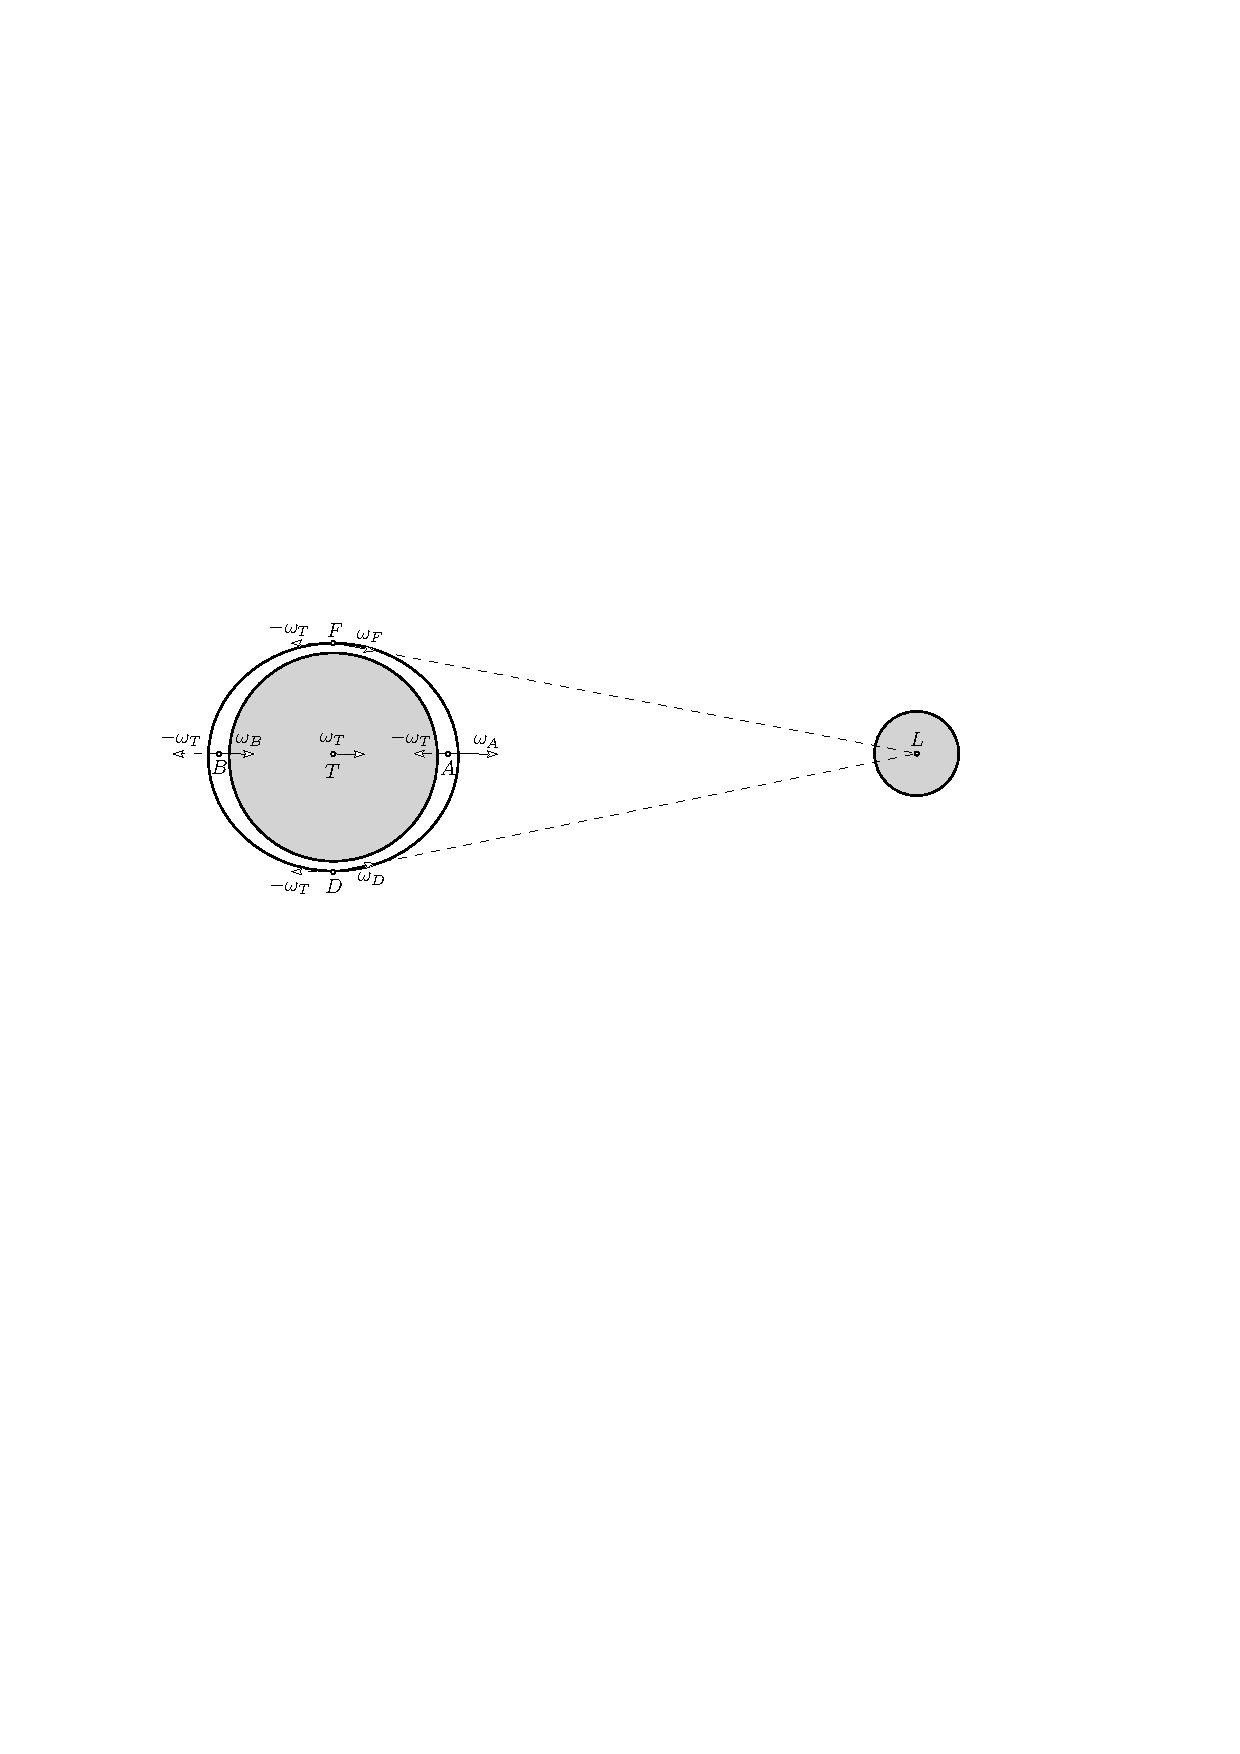
\includegraphics[width = \tw]{Ebb_flow}
	\captionof{figure}{К объяснению приливных сил}\label{Ebb_flow}
\end{minipage}\\[-0.5pc]

$r$~--- расстояние между центрами Земли и данного тела. Аналогично, ускорения в точках $A$ и $B$ равны соответственно
\begin{equation}
	a_A = \frac{G M}{(r - R)^2} \quad \text{и} \quad a_B = \frac{GM}{(r + R)^2},
\end{equation}
где $R$~--- радиус Земли или иного тела, подверженного воздействию приливных сил. Ускорение в точке $A$ относительно точки $T$ равно
\begin{equation}
    a_A - a_T = GM \cdot \frac{r^2 - (r - R)^2}{r^2 (r - R)^2} \xrightarrow{R \ll r} \frac{2 G M R}{r^3}.
	\label{eq:ebb-force}
\end{equation}

Под действием лунного притяжения водная оболочка Земли принимает форму
эллипсоида, который вытянут по направлению к Луне. Близ точек $A$ и $B$ будет
прилив, а в точках $F$ и $D$ --- отлив (см.~Рис.\,\ref{Ebb_flow}).

\subsection{Синодический период}
\label{sec:synodic-period}

\term{Синодический период} (период смены фаз) небесного тела~--- период относительного кругового движения.

В большинстве случаев имеется в виду относительное движение планет вокруг Солнца (А). Также может рассматриваться период смены фаз спутника планеты (Б) или период между последовательными пролетами спутника над одним и тем же меридианом планеты (В).

Важным понятием в определении синодического периода является \imp{относительная угловая скорость}~--- скорость увеличения углового разделения двух рассматриваемых объектов. Так в случае (A) это скорость изменения угла <<{\slshape одна планета\,--\,Солнце\,--\,другая планета}>>, в случае (Б)~--- угла <<{\slshape спутник\,--\,планета\,--\,Солнца}>>, наконец, в случае (В)~--- угла между отрезком <<{\slshape центр планеты\,--\,спутника}>> и меридианом планеты.

Численно относительная скорость равна разности угловых скоростей двух рассматриваемых движений.
\begin{equation*}
    \boldsymbol\omega_\text{отн} = \boldsymbol{\omega}_1 - \boldsymbol\omega_2.
\end{equation*} 
Обозначим за $S$ синодический период, тогда
\begin{equation*}
    \frac{2\pi}{S} = |\boldsymbol\omega_\text{отн}| = |\vec\omega_1 - \vec\omega_2| = \left| \frac{2\pi}{T_1} \pm \frac{2\pi}{T_2} \right|,
\end{equation*}
где выбор знака в последнем выражении зависит от взаимного направления векторов угловых скоростей, а значит от направления каждого из движений. Окончательно, для синодического периода верно,
\begin{equation}
    \frac{1}{S} = \left| \frac{1}{T_1} \pm \frac{1}{T_2} \right|.
\end{equation}
   
Для внешних и внутренних планет, соответственно, выражения принимают вид:
\begin{equation} \frac{1}{S} = \frac{1}{T_\oplus} - \frac{1}{T_\text{пл}} \quad \text{и} \quad \frac{1}{S} = \frac{1}{T_\text{пл}} - \frac{1}{T_\oplus},
\end{equation}
где $S$~--- синодический период, $T_\text{пл}$~--- сидерический период планеты, $T_\oplus$~--- сидерический период обращения Земли.

\begin{figure}[h!]
    \centering
    \begin{subcaptionblock}[t]{0.32\tw}
        \centering
        \tikzsetnextfilename{synodic-period-same-direction-outer}
        \begin{tikzpicture}
            \tkzDefPoint(0,0){S}
            \def\R{1.1}
            \def\r{0.8}
            \def\OMEGAIN{40}
            \def\OMEGAOUT{\OMEGAIN * (\R/\r) ^ (-3/2)}
            \tkzDefShiftPoint[S](0,\r){IN}
            \tkzDefShiftPoint[S](0,\R){OUT}

            \tkzDrawCircle[black,line width=0.4pt](S,IN)
            \tkzDrawCircle[black,line width=0.4pt](S,OUT)

            \tkzDrawArc[rotate, semithick, -latex](S,IN)(\OMEGAIN)
            \tkzDrawArc[rotate, semithick, -latex](S,OUT)(\OMEGAOUT)

            \sun(S)
            \earth(IN)
            \tkzDrawPoint(OUT)
        \end{tikzpicture}
        \caption{Схема относительного движения Земли и объекта на внешней орбите, движущегося в том же направлении, что и Земля}
    \end{subcaptionblock}
    \hfill
    \begin{subcaptionblock}[t]{0.32\tw}
        \centering
        \tikzsetnextfilename{synodic-period-same-direction-inner}
        \begin{tikzpicture}
            \tkzDefPoint(0,0){S}
            \def\R{1.1}
            \def\r{0.8}
            \def\OMEGAIN{40}
            \def\OMEGAOUT{\OMEGAIN * (\R/\r) ^ (-3/2)}
            \tkzDefShiftPoint[S](0,\r){IN}
            \tkzDefShiftPoint[S](0,\R){OUT}

            \tkzDrawCircle[black,line width=0.4pt](S,IN)
            \tkzDrawCircle[black,line width=0.4pt](S,OUT)

            \tkzDrawArc[rotate, semithick, -latex](S,IN)(\OMEGAIN)
            \tkzDrawArc[rotate, semithick, -latex](S,OUT)(\OMEGAOUT)

            \sun(S)
            \tkzDrawPoint(IN)
            \earth(OUT)
        \end{tikzpicture}
        \caption{Схема относительного движения Земли и объекта на внутренней орбите, движущегося в том же направлении, что и Земля}
    \end{subcaptionblock}
    \hfill
    \begin{subcaptionblock}[t]{0.32\tw}
        \centering
        \tikzsetnextfilename{synodic-period-opposite-direction}
        \begin{tikzpicture}
            \tkzDefPoint(0,0){S}
            \def\R{1.1}
            \def\r{0.8}
            \def\OMEGAIN{40}
            \def\OMEGAOUT{\OMEGAIN * (\R/\r) ^ (-3/2)}
            \tkzDefShiftPoint[S](0,\r){IN}
            \tkzDefShiftPoint[S](0,\R){OUT}

            \tkzDrawCircle[black,line width=0.4pt](S,IN)
            \tkzDrawCircle[black,line width=0.4pt](S,OUT)

            \tkzDrawArc[rotate, semithick, -latex](S,IN)(\OMEGAIN)
            \tkzDrawArc[rotate, semithick, latex-](S,OUT)(-\OMEGAOUT)

            \sun(S)
            \earth(IN)
            \tkzDrawPoint(OUT)
        \end{tikzpicture}
        \caption{Схема относительного движения Земли и объекта, движущегося в противоположном направлении, нежели Земля}
    \end{subcaptionblock}
    \caption{}
\end{figure}

В случае, если тела обращаются в противоположные стороны, связь
их синодического периода с сидерическими очевидным образом принимает вид:
\begin{equation}
    \frac{1}{S} = \frac{1}{T_1} + \frac{1}{T_2}.
\end{equation}

\begin{wrapfigure}[14]{r}{0.47\tw}
    \centering
    \vspace{-1pc}
    \tikzsetnextfilename{sinodic-period-plot}
    \begin{tikzpicture}
        \begin{axis}[
            width    =    6cm,
            height    =    6cm,
            xlabel    =    {$T_2 / T_1$},
            ylabel    =    {$S / T_1$},
            ymax    =    6,
            ymin    =    0,
            xmax    =    6,
            xmin    =    0,
            legend cell align=left,
            legend style={
                row sep = 0.8pc,
                draw=none,
                fill=none,
                font=\scriptsize,
                at={(axis cs:2.5, 5.5)}, anchor=north west,
            },
        ]
            \addplot [domain=0:1, samples=100, black] {-1 / (1 - 1 / x)};
            \addplot [domain=1:6, samples=100, dash pattern=on 6pt off 2pt on 1pt off 2pt] {1 / (1 - 1 / x)};
            \addplot [domain=0:6, samples=100, dash pattern=on 6pt off 2pt on 1pt off 2pt on 1pt off 2pt] {1 / (1 + 1 / x)};

            \addplot [dashed, line width=0.5pt] coordinates { (1,0) (1,6) };
            \addplot [dashed, line width=0.5pt] coordinates { (0,1) (6,1) };

            \legend{
                $\dfrac{1}{T_1/T_2 - 1}$,
                $\dfrac{1}{1 - T_1/T_2}$,
                $\dfrac{1}{1 + T_1/T_2}$
            }
        \end{axis}
    \end{tikzpicture}
    \caption{}
    \label{pic:sinodic-period-plot}
\end{wrapfigure} 
На~\picRef{pic:sinodic-period-plot} изображены зависимости продолжительности синодического периода от отношения периодов планет. Важно обратить внимание на вертикальную асимптоту, к которой стремится график в случае движения планет в одну сторону вокруг Солнца. Она отражает отсутствие смены фаз в случае движения объектов по одной круговой орбите.

Горизонтальная асимптота является следствием стремления синодического периода к сидерическому периоду наблюдателя при стремлении сидерического периода объекта к бесконечности. При этом в случае сонаправленного движения синодический период приближается к сидерическому периоду наблюдателя сверху, а в случае встречного~--- снизу.

{\footnotesize Рассмотрим подробнее описанные выше случаи на конкретных примерах.\newline
{\bfseries (A) Относительное движение двух планет вокруг Солнца.} Для анализа возьмем пару Земля и Венера. Период Земли $T_\oplus = 1$~год, Венеры~--- $T_{\venus} = 0.62$~года. Следовательно, синодический период (период смены фаз) Венера для земного наблюдателя, также синодический период Земли для наблюдателя на Венера, определяется как
\begin{equation*}
    \frac{1}{S_{\oplus\venus}} = \left| \frac{1}{T_\oplus} - \frac{1}{T_{\venus}} \right| = \frac{1}{T_{\venus}} - \frac{1}{T_\oplus} = \frac{1}{0.62~\text{года}} - \frac{1}{1~\text{год}} = 0.61~\frac{1}{\text{год}}~~\Rightarrow~~S_{\oplus\venus} = 1.63~\text{года},
\end{equation*}
важно отметить, что здесь имеется в виду не календарный, а сидерический год Земли.\newline
{\bfseries (Б) Период смены фаз спутника планеты.} Найдём период смены фаз естественного спутника Земли~--- Луны. Движения, рассматриваемые в данном примере, это обращение Луны вокруг Земли с сидерическим периодом Луны $T_{\rightmoon} = 27.3$~суток и обращение Земли вокруг Солнца с сидерическим периодом Земли $T_\oplus \simeq 365$~суток. Следовательно, период смены фаз Луны
\begin{equation*}
    S_{\rightmoon} = \left| \frac{1}{T_\oplus} - \frac{1}{T_{\rightmoon}}\right|^{-1} = \left(\frac{1}{T_{\rightmoon}} - \frac{1}{T_\oplus}\right)^{-1} = \left(\frac{1}{27.3} - \frac{1}{365}\right)^{-1} = 29.5~\text{суток}.
\end{equation*}
{\bfseries (В) Орбитальное движение и вращение вокруг своей оси.} Несколько переиначим пример описанный выше: рассмотрим движение Земли вокруг Солнца и суточное вращение Земли вокруг своей оси, найдём продолжительность солнечных суток на Земле. Сидерический период Земли $T_\text{орб} \simeq 365$~суток (солнечных), а звёздные сутки $T_\text{ос} = 23^\text{h}\,56^\text{m}\,4^\text{s}$. Отсюда,
\begin{equation*}
    T_\text{сут} = \left(\frac{1}{T_\text{ос}} - \frac{1}{T_\text{орб}}\right)^{-1} = 24~\text{часа}.
\end{equation*}}

\subsubsection*{Либрация}

\begin{wrapfigure}[15]{r}{0.52\tw}
    \centering
    \vspace{-1pc}
    \tikzsetnextfilename{libration-plot}
     \begin{tikzpicture}
        \begin{axis}[
            width     =    6cm,
            height    =    6cm,
            ymax    =    3.142,
            xmax    =    6.284,
            xmin    =    0,
            ymin    =   -3.142,
            xlabel    =    {$M$},
            ylabel     =     {$\nu - M$},
            legend cell align=left,
            legend style={
                draw=none,
                fill=white,
                font=\scriptsize,
                at={(axis cs:3.5, 3)}, anchor=north west,
            },
            legend image post style={
                minimum height=0.75em,
                minimum width=3.5em,
            },
            xtick={0, pi / 2, pi, 3 * pi / 2, 2 * pi}, 
            xticklabels={$0$, $\pi / 2$, $\pi$, $3\pi / 2$, $2\pi$},
            ytick={-pi, -pi / 2, 0, pi / 2, pi}, 
            yticklabels={$-\pi$, $-\dfrac{\pi}{2}$, $0$, $\dfrac{\pi}{2}$, $\pi$},
        ]
            \addplot[smooth,dash pattern=on 6pt off 2pt on 1pt off 2pt on 1pt off 2pt on 1pt off 2pt] table[x=m, y=e01] {data/libration.txt};
            \addplot[smooth,dash pattern=on 6pt off 2pt on 1pt off 2pt on 1pt off 2pt] table[x=m, y=e03] {data/libration.txt};
            \addplot[smooth,dash pattern=on 6pt off 2pt on 1pt off 2pt] table[x=m, y=e05] {data/libration.txt};
            \addplot[smooth,dash pattern=on 6pt off 2pt] table[x=m, y=e07] {data/libration.txt};
            \addplot[smooth] table[x=m, y=e09] {data/libration.txt};

            \legend{
                $e=0.1$,
                $e=0.3$,
                $e=0.5$,
                $e=0.7$,
                $e=0.9$,
            }
        \end{axis}
    \end{tikzpicture}
    \caption{}
    \label{pic:libration-plot}
\end{wrapfigure}
Tермин \term{либрация} в астрономии используется для описания влияния неравномерности орбитального движения спутника его на видимое вращение, которое происходит в постоянной угловой скоростью. В случае сихрнонизации орбитального движения спутника и его вращения вокруг оси, например, Луна, либрация позволяет наблюдателю на Земле видеть более половины поверхности спутника. 

Так как вращение спутника вокруг своей оси происходит с постоянной угловой скоростью, то оно линейным образом зависит от средней аномалии $M$ спутника. При этом средняя аномалия связана с эксцентрической аномалией $E$ уравнением Кеплера \eqref{eq:kepler-eq-E-nu-2}. Которая в свою очередь описывать истинную аномалию $\nu$, определяющую положение тела на орбите и, соотвветственно, его поворот относительно наблюдателя в следствии орбитального движения.

Выразим эксцентрическую аномалию $E$ как функцию от средней аномалии $M$. Для этого воспользуемся методом неподвижной точки\,\cite{balk_dynamic_space_flight}. Пусть $E_0 = 0$, а $E_{n+1} = e \sin E_n + M$, такая последовательность сходится, см.~\cite{balk_dynamic_space_flight}. Не сложно  получить, что
\begin{equation*}
    E_n = M + e \sin \big( M + e \sin ( M + \ldots) \big).
\end{equation*}
Далее преобразуем \eqref{eq:kepler-eq-E-nu-2}, чтобы получить выражение для $nu$:
\begin{equation*}
    \nu = 2 \arctg \left( \tg \frac{E}{2} \sqrt{\frac{1 + e}{1 - e}} \right).
\end{equation*}

Разность $\nu - M$ определяет разность между наблюдаемой ориентацией спутника и ориентацией в случае круговой орбиты. График зависимости $\nu - M$ от $M$ или, что тоже самое, от части периода спутника приведем на \picRef{pic:libration-plot} для различных величин эксцентриситета $e$.



\subsection{Ретроградное движение и точки стояния}
Рассмотрим характер движения планеты по небесной сфере в течение синодического периода. Пусть \imp{наблюдатель}~--- условная точка, обращающаяся вокруг Солнца по некоторой круговой орбите, согласно законам Кеплера. Назовем \imp{лучем зрения} прямую, проходящую через наблюдателя и наблюдаемую планету. Тогда угловая скорость планеты на небесной сфере наблюдателя $\boldsymbol \omega = \cross{(r_\text{п} - r_\text{н})}{(u - v)}$, где $\vec{u}$ и $\vec{v}$~--- векторы орбитальных скоростей планеты и наблюдателя соответсвенно. 

Пусть планета является внешней для наблюдателя, случай внутренней рассматривается аналогично. Найдём угловую скорость планеты в противостоянии и соединении:
\begin{align*}
    \omega_\text{п} &= \frac{u - v}{a_\text{п} - a_\text{н}} < 0,\\ 
    \omega_\text{с} &= \frac{u + v}{a_\text{п} + a_\text{н}} > 0,
\end{align*}
где в качестве положительного направления выбрано направления движения Солнца на небе наблюдателя. 

Из геометрического смысла и определения угловой скорости очевидно, что это непрерывная функция, а значит, существуют такие моменты, когда планета меняет направление своего видимого движения по небесной сфере наблюдателя, такие точки называются \term{точками стояния}. А движение планеты в противоположную движению Солнца сторону~--- \term{ретроградным движением}. Причём внешние планеты находятся в ретроградном движении в окрестности противостояния, а внутренние~--- в окрестности нижнего соединения.

Получим выражение для размера петли ретроградного движения планеты. Для простоты изложения положим, что планета является внешней. В конце покажем, что полученное выражение справедливо и для внутренних планет. 

Итак, пусть обиты планеты и наблюдателя круговые с радиусами $a_\text{п}$ и  $a_\text{н}$ соответственно, пусть также $\alpha$~--- разность эклиптических долгот наблюдателя и планеты, \lookPicRef{???}. Тогда расстояние $r$ между ними можно найти из теоремы косинусов:
\begin{equation}
    r = \sqrt{a_\text{п}^2 + a_\text{н}^2 - 2 a_\text{п} a_\text{н} \cos \alpha}.
    \label{eq:retrograde-movement-distance}
\end{equation}

Пусть $\delta$~--- угол Солнце~-- планета~-- наблюдатель, запишем теорему синусов:
\begin{equation}
    \frac{a_\text{н}}{\sin \delta} = \frac{r}{\sin \alpha}.
    \label{eq:retrograde-movement-sinuses-theorem}
\end{equation}
Остается сказать, что обнуление видимой угловой скорости планеты происходит при равенстве проекций скоростей планеты и наблюдателя на нормаль к лучу зрения, что эквивалентно
\begin{equation}
    v \cos (\alpha + \delta) = u \cos \delta.
    \label{eq:retrograde-movement-velocity-projectione-equivalence}
\end{equation}

Найдём теперь $\alpha$ из системы уравнений \eqref{eq:retrograde-movement-distance}\,--\,\eqref{eq:retrograde-movement-velocity-projectione-equivalence}. Для удобства изложения введём обозначение $b \equiv a_\text{п} / a_\text{н} > 1$. И начнём с \eqref{eq:retrograde-movement-sinuses-theorem}, откуда выразим $\sin \delta$:
\begin{multline*}
    \sin \delta 
        = \frac{a_\text{н} \sin \alpha}{r} 
        = \frac{a_\text{н} \sin \alpha}{\sqrt{a_\text{п}^2 + a_\text{н}^2 - 2 a_\text{п} a_\text{н} \cos \alpha}} = \\
        =  \frac{a_\text{н} \sin \alpha}{a_\text{н} \sqrt{1 + \dfrac{a_\text{п}^2}{a_\text{н}^2} - 2 \dfrac{a_\text{п}}{a_\text{н}} \cos \alpha}}
        = \frac{\sin \alpha}{\sqrt{1 + b^2 - 2 b \cos \alpha}}.
\end{multline*}
Далее получим выражение для $\cos \delta$ из основного тригонометрического тождества:
\begin{multline*}
    0 < \cos \delta 
        = \sqrt{1 - \sin^2 \delta} 
        = \sqrt{1 - \frac{\sin^2 \alpha}{1 + b^2 - 2 b \cos \alpha}} = \\
        = \sqrt{\frac{1 + b^2 - 2 b \cos \alpha - 1 + \cos^2 \alpha}{1 + b^2 - 2 b \cos \alpha}}
        = \frac{b - \cos \alpha}{\sqrt{1 + b^2 - 2 b \cos \alpha}}
\end{multline*}
Также вспомним, что
\begin{equation*}
    \frac{u}{v} = \frac{\sqrt{\dfrac{GM_\odot}{a_\text{п}}}}{\sqrt{\dfrac{GM_\odot}{a_\text{н}}}} = \sqrt{\frac{a_\text{н}}{a_\text{п}}} \equiv \sqrt{\frac{1}{b}}.
\end{equation*}
Остаётся раскрыть косинус суммы в \eqref{eq:retrograde-movement-velocity-projectione-equivalence}:
\begin{gather}
    v (\cos \alpha \cos \delta - \sin \alpha \sin \delta) = u \cos \delta,\nonumber\\
    \cos \alpha \cos \delta - \sin \alpha \sin \delta = \sqrt{\frac{1}{b}} \cos \delta,\nonumber\\
    \cos \delta \left( \cos \alpha - \sqrt{\frac{1}{b}} \right) = \sin \alpha \sin \delta,\nonumber\\
    \frac{b - \cos \alpha}{\sqrt{1 + b^2 - 2 b \cos \alpha}}\left( \cos \alpha - \sqrt{\frac{1}{b}} \right) = \sin \alpha \frac{\sin \alpha}{\sqrt{1 + b^2 - 2 b \cos \alpha}},\nonumber\\
    b \cos \alpha - \sqrt{b} - \cos^2 \alpha + \sqrt{\frac{1}{b}} \cos \alpha = 1 - \cos^2 \alpha,\nonumber\\
    \cos \alpha = \frac{b + \sqrt{b}}{b \sqrt{b} + 1}.
    \label{eq:retrograde-movement-alpha}
\end{gather}
Вторая точка стояния определяется той же разницей долгот, что видно из \picRef{???}, следовательно, ретроградное движение планеты происходит на протяжении времени
\begin{equation*}
    t 
        = \frac{2 \alpha}{|\omega_\text{н} - \omega_\text{п}|} 
        = \frac{2 \alpha}{\left|\dfrac{2\pi}{T_\text{н}} - \dfrac{2\pi}{T_\text{п}} \right|} 
%        = \frac{\alpha}{\pi} \cdot \frac{T_\text{п} T_\text{н}}{T_\text{п} - T_\text{н}} = \\
        = \frac{\alpha}{\pi}\cdot \frac{T_\text{п}}{\left|\dfrac{T_\text{п}}{T_\text{н}} - 1\right|} 
        = \frac{\alpha}{\pi}\cdot \frac{T_\text{п}}{\left| b \sqrt{b} - 1 \right|}.
\end{equation*}
А планета за это время проходит по орбите угол
\begin{equation*}
    \psi = t \omega_\text{п} = \frac{\alpha}{\pi} \cdot \frac{T_\text{п}}{b \sqrt{b} - 1} \cdot \frac{2\pi}{T_\text{п}} = \frac{2\alpha}{b \sqrt{b} - 1}.
\end{equation*}
Остается отметить, размер петли попятного движения $\Delta \lambda = 2\delta - \psi$, что следует из \picRef{???}. Чтобы получить аналитический вид данного выражения, найдем
\begin{multline*}
    \cos 2 \delta 
        = 1 - 2 \sin^2 \delta 
        = 1 - \frac{2(1 - \cos^2 \alpha)}{1 + b^2 - 2b \cos \alpha} = \\
        =\frac{1 + b^2 - 2 b \cos \alpha - 2 + 2 \cos^2 \alpha}{1 + b^2 - 2b\cos \alpha} =\\
        = \frac{-1 + b^2 - 2b \cdot \dfrac{b + \sqrt{b}}{b \sqrt{b} + 1} + 2 \cdot \dfrac{b^2 + b +2b\sqrt{b}}{b^3 + 1 + 2 b \sqrt{b}}}{1 + b^2 - 2b \cdot \dfrac{b + \sqrt{b}}{b \sqrt{b} + 1}}\\
%        = \frac{\dfrac{\scriptstyle{-b^3 - 1 - 2b\sqrt{b} + b^5 + b^2 + 2b^3\sqrt{b} - 2b^3 \sqrt{b} - 2b^3 - 2b^2 - 2b\sqrt{b} + 2b^2 + 2b + 4b\sqrt{b}}}{\scriptstyle{\left(b \sqrt{b} +1\right)^2}}}{\dfrac{\scriptstyle{b\sqrt{b} + 1 + b^3 \sqrt{b} + b^2 - 2b^2 - 2b\sqrt{b}}}{\scriptstyle{b \sqrt{b} + 1}}} = \\
        = \frac{-1 + 2b + b^2 - 3b^3 + b^5}{\left(b \sqrt{b} + 1\right) \left(1 - b \sqrt{b} - b^2 + b^3 \sqrt{b}\right)} = \\
        = \frac{(b^2 - 1) - 2b(b^2 - 1) + b^3(b^2 - 1)}{(1 - b^3)(1 - b^2)} = \\
        = \frac{1 - 2b + b^3}{b^3 - 1} = \frac{b^2(b-1) + b(b-1) - (b - 1)}{\left(b-1\right)\left(b^2 + b + 1\right)} = \frac{b^2 + b - 1}{b^2 + b + 1}.
\end{multline*} 
Отсюда, размер петли
\begin{equation}
    \Delta\lambda = \arccos \frac{b^2 + b - 1}{b^2 + b + 1} - \frac{2}{\left|b\sqrt{b} - 1 \right|} \cdot \arccos \frac{b + \sqrt{b}}{b \sqrt{b} + 1}.
\end{equation}

\begin{wrapfigure}[9]{r}{0.47\tw}
	\centering
	\vspace{-1pc}
	\begin{tikzpicture}
		\begin{axis}[
			width	=	.5\tw,
			height	=	4.5cm,
			xlabel	=	{$b$},
			ylabel	=	{$\Delta \lambda, ~^\circ$},
%			ymax	=	1,
			ymin	=	0,
			xmax	=	10,
			xmin	=	0,
			legend cell align=left,
			legend style={
				row sep = 1mm,
				draw=none,
				fill=none,
				font=\scriptsize,
				at={(axis cs:1.2, 2.5)}, anchor=south west,
			},
		]
			\addplot [domain=0:10, samples=37, smooth] {acos((x^2 + x - 1)/(x^2 + x + 1)) - 2 / abs(x*sqrt(x) - 1) * acos((x + sqrt(x))/(x * sqrt(x) + 1))};
			\addplot[mark=o, only marks, black, mark options={
        scale=0.75, fill=white}]  coordinates {(0.42, 14.2) (0.72,16.15) (1.52,15.93) (5.2,9.95) (9.6,6.76)};
			\legend{
				$\Delta \lambda(b)$,
				Планеты Сол.\,сист.
			}
		\end{axis}
	\end{tikzpicture}
	\caption{}
\end{wrapfigure}
Легко заметить, что для внутренней планеты результат будет тот же, стоит только поменять местами индексы наблюдателя и планеты в вкладках выше. 









\subsection{Прецессия}
\begin{wrapfigure}[15]{l}{0.41\tw}
	\vspace{-1pc}
	\centering
	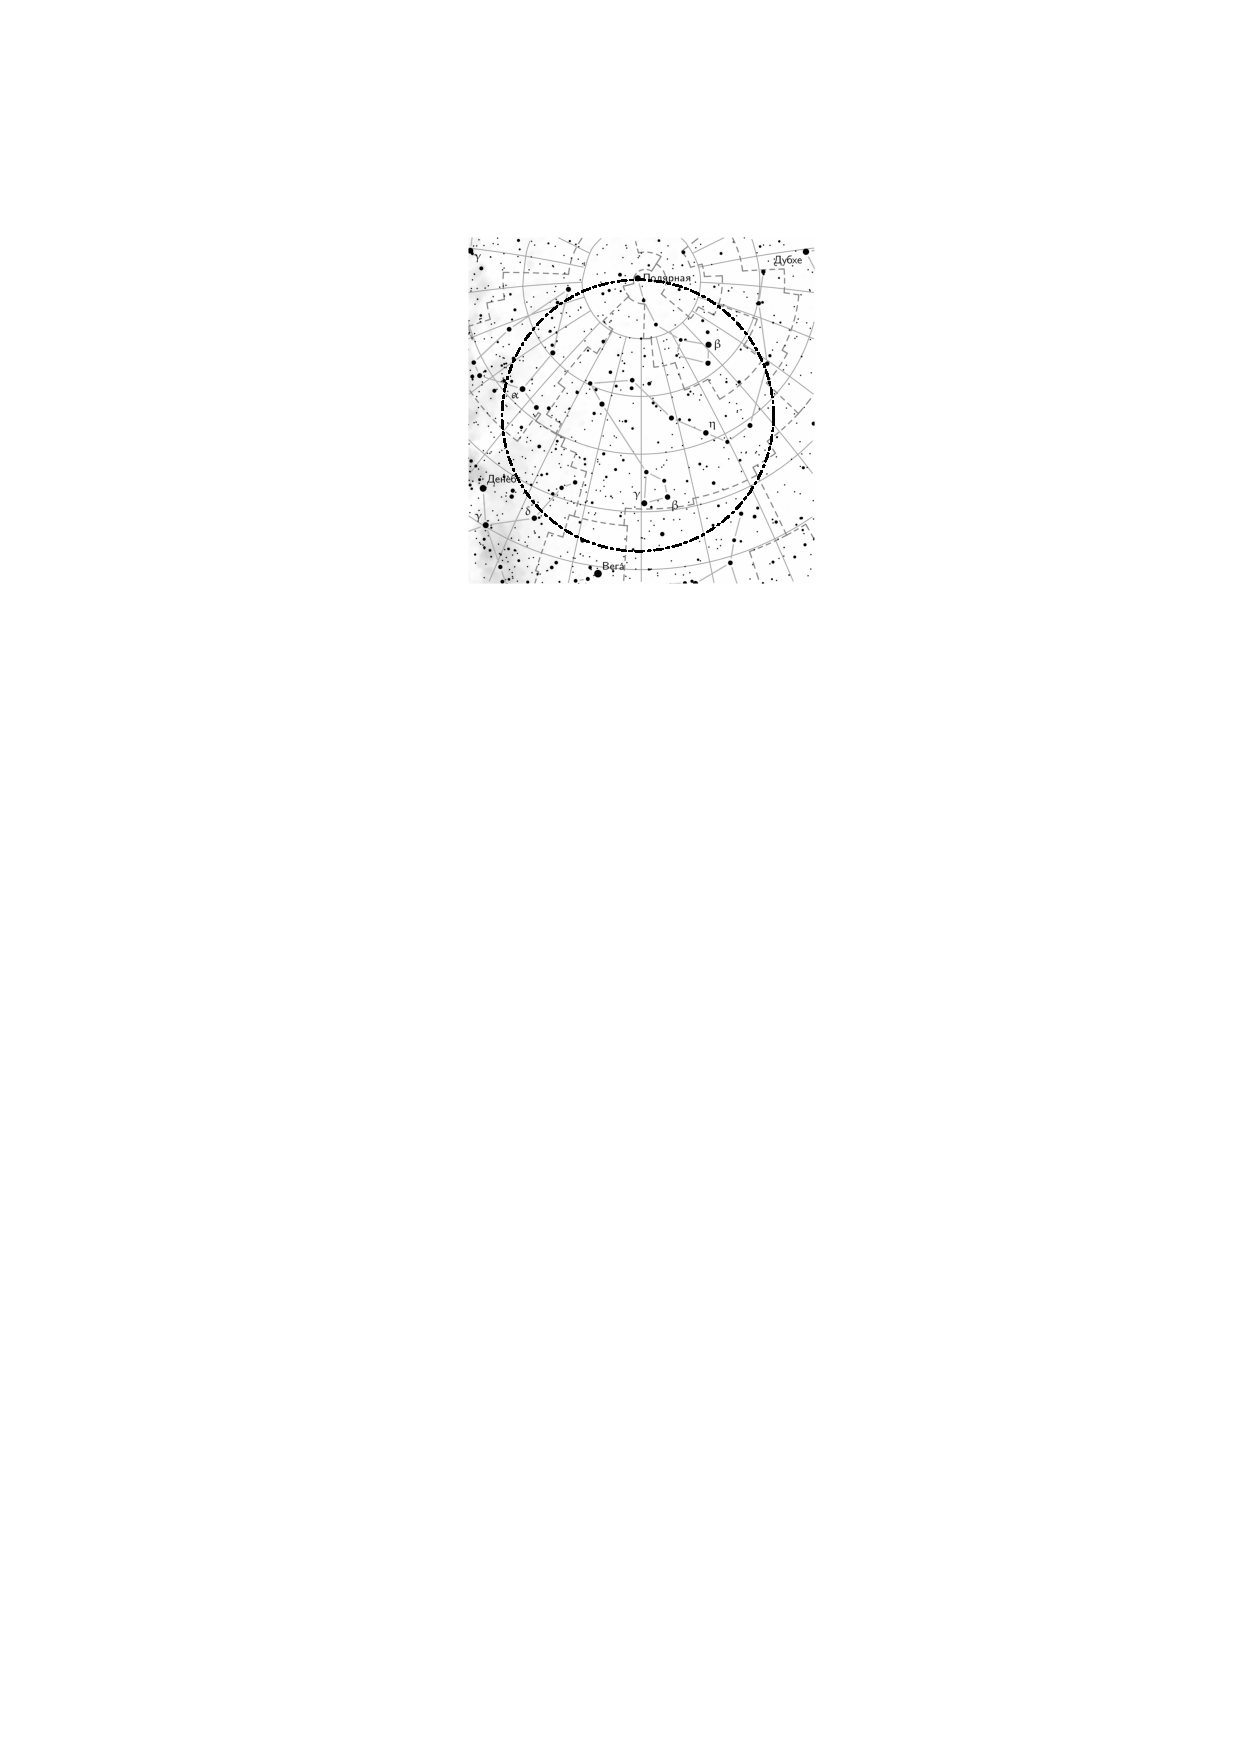
\includegraphics[width = .42\tw]{precession_bw}
	\caption{Прецессионное движение северного полюса мира}
	\label{fig:precession-path}
\end{wrapfigure}
Под действием возмущающих сил ось вращения Земли совершает прецессионное движение: описывает вокруг оси эклиптики конус с углом раствора $23.5^\circ$ с периодом около  25\,765~лет. Из-за этого меняется положение полюса мира. Например, сейчас полюс мира практически совпадает с Полярной звездой ($\alpha$\,UMi), а 15\,000~лет назад роль полярной звезды играла Вега ($\alpha$\,Lyr). Если считать, что величина прецессии постоянна, то полюсы мира описывают вокруг полюсов эклиптики малые круги с радиусом $23.5^\circ$. В~действительности~же величина прецессии меняется, поэтому путь полюсов мира представляет собой не~окружность, а~спираль.

Поворот оси Земли имеет различные последствия. Во-первых, меняется продолжительность тропического года, он становится примерно на $20$~минут короче звёздного, во-вторых, меняется вид звёздного неба  (см.~Рис.\,\ref{fig:precession-path}).

	\section{Конические сечения}
\subsection{Эллипс}

{\bfseries \term{Эллипс}}~--- плоская замкнутая кривая, сумма расстояний от любой точки которой до двух фиксированных точек, называемых фокусами, постоянна.
\begin{equation}
	|F_1 M| + |F_2 M|=\const \label{eq:ell-def}
\end{equation}
\imp{Центром} эллипса называется середина отрезка, соединяющего его фокусы.

\imp{Большая ось} эллипса~--- прямая, проходящая через фокусы эллипса; \imp{малая ось}~--- прямая ей перпендикулярная и проходящая через центр эллипса.

\begin{wrapfigure}[10]{r}{0.5\tw}
    \vspace{-1pc}
	\centering
	 \begin{tikzpicture}
       \pgfmathsetmacro\a{2}
	   \pgfmathsetmacro\e{0.7}
	   \pgfmathsetmacro\b{\a * sqrt(1 - \e^2)}
	   \pgfmathsetmacro\c{\a * (1 - \e)} 
	   
	   \tkzDefPoint(\a,0){X0}
	   \foreach \nu in {0,0.05,...,6.4} {
	       \def\x{\a * cos(\nu)}
	       \def\y{\a * sin(\nu) * sqrt(1 - \e * \e)}
	       \tkzDefPoint(\x,\y){X1}
	       \tkzDrawSegment[thick](X0,X1)
	       \tkzDefShiftPoint[X1](0,0){X0}
	   }
	   
	   \tkzDefPoint(0,0){O}
	   \tkzDefPoint({-\a*\e},0){F1}
	   
	   \tkzDefPointBy[homothety=center O ratio -1](F1) \tkzGetPoint{F2}
	   
	   \tkzDefPointBy[homothety=center O ratio 1/\e](F1) \tkzGetPoint{Q1}
	   \tkzDefPointBy[homothety=center O ratio 1/\e](F2) \tkzGetPoint{Q2}
	   
	   \tkzDefPointWith[orthogonal,K={-1/\e+\e}](F2,O) \tkzGetPoint{P}
	   
	   \tkzDefPointWith[orthogonal,K={sqrt(1-\e*\e)}](O,Q1) \tkzGetPoint{B1}
	   \tkzDefPointWith[orthogonal,K={sqrt(1-\e*\e)}](O,Q2) \tkzGetPoint{B2}
	   
	   \tkzDrawSegments[thick](Q1,Q2 F1,P P,F2 B1,O F1,B1 B1,F2)
	   
	   \tkzLabelPoint[above=-1pt](F1){\adjustbox{right=10pt}{$\mathbf{F_1}$}}
	   \tkzLabelPoint[above right=-2pt](F2){$\mathbf{F_2}$}
	   \tkzLabelPoint[above](O){$\mathbf{O}$}
	   
	   \tkzLabelSegment[above=2pt](F1,P){$2a-p$}
	   \tkzLabelSegment[below left=-3pt](F1,B1){$a$}
	   \tkzLabelSegment[below right=-3pt](F2,B1){$a$}
	   
	   \tkzMarkRightAngles[size=0.15](P,F2,O B1,O,F2)
	   
	   \def\k{0.2}
	   
	   \tkzDrawSegment[dim={$p$, \fpeval{\c+\k}cm, right=1mm}](P,F2)
	   
	   \tkzDrawSegment[dim={$b$, \fpeval{\a+\k}cm, left=1mm}](B1,O)

	   \tkzDrawSegment[dim={$a$, \fpeval{\b + \k}cm, below=1mm}](Q2,O)
	   \tkzDrawSegment[dim={$c$, \fpeval{\b + \k}cm, below=1mm}](O,F1)
	   \tkzDrawSegment[dim={$Q$, \fpeval{\b + 3*\k}cm, below=1mm}](Q2,F1)
	   \tkzDrawSegment[dim={$q$, \fpeval{\b + 3*\k}cm, below=1mm}](F1,Q1)
	   
	   \tkzDrawPoints(O, F1, F2, Q1, Q2, B1, P)     
    \end{tikzpicture}
	\caption{Эллипс}
	\label{pic:ellipse}
\end{wrapfigure}
Главные отрезки эллипса: \term{боль\-шая полуось} ($a$)~--- расстояние от центра эллипса до его пересечения с большой осью; \term{малая полуось} ($b$) определяется дословно также, заменив большую ось на малую; \term{фокальное расстояние} ($c$)~--- расстояние от центра эллипса до одного из фокусов, что тоже самое, половина расстояния между фокусами.

Рассмотрим крайнюю левую и крайнюю правую точки эллипса на Рис.~\ref{pic:ellipse}, назовем их $A$ и $B$ соответственно, тогда сумма расстояний $l$ от каждой из них до фокусов $F_1$ и $F_2$ равна:
\begin{equation*}
	AF_1 + AO + OF_2 = AF_1 + a + c = l = BF_2 + BO + OF_1 = BF_2 + a + c.
\end{equation*}
Откуда следует, что $A F_1 = B F_2$. Легко видеть, что $AB = 2a$, значит $l = AF_1 + AO + OF_2 = AO + OF_2 + F_2B = 2a$. Получается, сумма расстояний до фокусов от любой точки эллипса равна его удвоенной большой полуоси.

В силу равенства прямоугольных треугольников $\triangle F_1 O C$ и $\triangle F_2 O C$ равны их гипотенузы $F_1C$ и $F_2C$, причем $F_1C= F_2C = l/2 = a$. Отсюда получается одно из основных соотношений в эллипсе:

\begin{equation}
	b^2 + c^2 = a^2.
\end{equation}
\term{Эксцентриситет} ($e$)~--- числовая
характеристика, показывающая степень отклонения конического сечения от окружности. Для эллипса $e$ лежит в интервале $(0, \, 1)$ и
определяется формулой
\begin{equation}
	e = \frac{c}{a}.
\end{equation}

\term{Апоцентр}~--- наиболее удаленная от заданного фокуса точка эллипса. Расстояние $Q$ до апоцентра от фокуса~--- сумма расстояний от фокуса, до центра эллипса и расстояния от центра до апоцентра, т.\,е.

\begin{equation}
	Q = c + a = a (1 + e).
\end{equation}

\term{Перицентр}~--- ближайшая точка эллипса к заданному фокусу. По аналогии с апоцентром, для расстояния $q$ от фокуса эллипса до перицентра справедливо следующее:
\begin{equation}
	q = a - c = a (1 - e).
\end{equation}

\term{Фокальный параметр}~($p$)~--- длина перпендикуляра, проведенного из фокуса до точки пересечения с эллипсом. Найдем $p$ из теоремы Пифагора для треугольника $\triangle F_1 F_2 P$:
\begin{gather}
	p^2 = (2a - p)^2 - (2c)^2, \notag\\
	p^2 =  4a^2 - 4ap + p^2 - 4a^2e^2,\notag\\
%	0 = a ( 1 - e^2) - p,\notag\\
	\therefore p = a (1 - e^2) = \frac{b^2}{a} = b \sqrt{1 - e^2}.
\end{gather}


\begin{wrapfigure}{r}{0.45\tw}
	\centering
	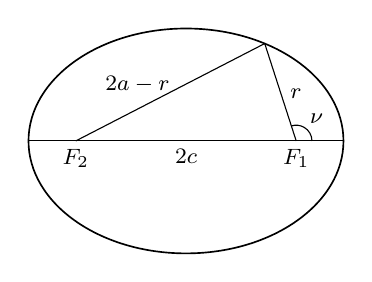
\begin{tikzpicture}[scale=1]
		\footnotesize
		
		\coordinate (O) at (0, 0);
		\coordinate (xy) at (1, 1.237);
		\coordinate (F1) at (1.4, 0);
		\coordinate (F2) at (-1.4, 0);
		
		\draw [semithick] (O) ellipse(2 and 1.428);
		
		\draw  (-2, 0) -- (2, 0);
		
		\draw (F1) -- (xy) -- (F2);
		
		\draw ([shift=(0:0.2)] F1) arc(0:108:0.2);
		
		\draw (F1) node [anchor=north] {$F_1$};
		\draw (F2) node [anchor=north] {$F_2$};
		\draw (1.47, 0.12) node [anchor=south west] {$\nu$};
		\draw (O) node[anchor=north] {$2c$};
		\draw (1.22, 0.6) node[anchor=west] {$r$};
		\draw (-0.1, 0.72) node[anchor=east] {$2a-r$};
		
		\point (F1);
		\point (F2);
		\point (xy);
	\end{tikzpicture}
	\caption{}
\end{wrapfigure}
Получим теперь выражение для расстояния от произвольной точки эллипса с \term{истинной аномалией}~$\nu$~--- угол
{\slshape перицентр -- фокус -- заданная точка},
отсчитываемый в сторону движения по эллипсу. Для этого необходимо рассмотреть треугольник {\slshape перицентр -- фокус -- заданная точка} и записать для него теорему косинусов:
\begin{gather*}
	(2a - r)^2 = r^2 + (2c)^2 - 2 r \cdot 2c \cos (180^\circ - \nu),\\
	4a^2 - 4ar + r^2 = r^2 + 4 a^2 e^2 + 4 r a e \cos \nu,\\
%	a - r = ae^2 + re\cos \nu,\\
	\therefore r = \frac{a(1 - e^2)}{1 + \cos \nu}.
\end{gather*}
Полученное выражение для длины радиус-вектора точки на эллипсе в зависимости от ее угла от перицентра называется \term{уравнением эллипса в полярных координатах}. Если же полюс системы координат расположить в другом фокусе, тогда полярный угол будет, очевидно, отсчитываться от точки апоцентра и в знаменателе уравнения будет знак <<$-$>>. Окончательно,
\begin{equation}
	r = \frac{a ( 1- e^2)}{1 \pm e \cos \nu}.
	\label{eq:ell-eq-pol}
\end{equation}

Перейдем теперь в декартовы координаты, в которых $r = \sqrt{x^2 + y^2}$, а $\cos \nu = x / r$, тогда:
\begin{gather*}
	\sqrt{x^2 + y^2} = \frac{a(1 - e^2)}{1 + e \cdot \dfrac{x}{\sqrt{x^2 + y^2}}} = \frac{a (1 - e^2) \sqrt{x^2 + y^2}}{\sqrt{x^2 + y^2} + e x},\\
	\sqrt{x^2 + y^2} = a(1 - e^2) - e x,\\
	x^2 + y^2 = a^2 (1 - e^2)^2 + e^2 x^2 - 2ae(1 - e^2) x,\\
	(1 - e^2) x^2 + y^2 = a^2 (1 - e^2)^2 - 2ae (1 - e^2) x,\\
	x^2 + \frac{y^2}{1 - e^2} = a^2 (1 - e^2) - 2aex.
\end{gather*}
\begin{wrapfigure}{r}{0.45\tw}
	\centering
	\vspace{-2pc}
	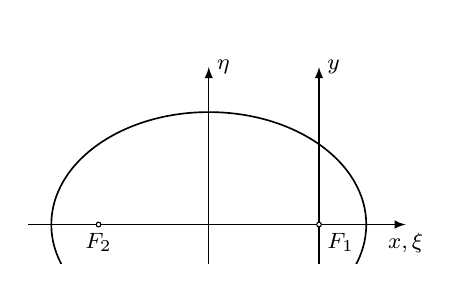
\begin{tikzpicture}[scale=1]
		\footnotesize
		
		\clip (-2.3, -0.5) rectangle (3, 2.5);
		
		\coordinate (O) at (0, 0);
		\coordinate (xy) at (1, 1.237);
		\coordinate (F1) at (1.4, 0);
		\coordinate (F2) at (-1.4, 0);
		
		\draw [semithick] (O) ellipse(2 and 1.428);
		
		\draw [-latex] (0, -1.7) -- (0, 2);
		\draw [-latex] (1.4, -1.7) -- (1.4, 2);
		\draw [-latex] (-2.3, 0) -- (2.5, 0);
		
%		\draw [-latex, thick] (xy) -- (F1);
%		\draw [-latex, thick] (xy) -- (F2) ;
%		\draw [-latex, thick] (xy) -- (2, 0.825);
%		\draw [dashes] (-1, 2.062) -- (2.5, 0.618);
		
%		\draw ([shift=(-72:0.3)] xy) arc(-72:-22.4:0.3);
%		\draw ([shift=(157.6:0.3)] xy) arc(157.6:207.3:0.3);

		\draw (F1) node [anchor=north west] {$F_1$};
		\draw (F2) node [anchor=north] {$F_2$};
%		\draw (1.2, 0.6) node [anchor=west] {$\vec r_1$};
%		\draw (-0.2, 0.63) node [anchor=south] {$\vec r_2$};
%		\draw (1.505, 1) node [anchor=south] {$\vec t$};

		\draw (2.5, 0) node [anchor=north] {$x, \xi$};
		\draw (1.4, 2) node [anchor=west] {$y$};
		\draw (0, 2) node [anchor=west] {$\eta$};
		
		\draw (F1) [fill=white] circle(.03);
		\draw (F2) [fill=white] circle(.03);
%		\draw (xy) [fill=white] circle(.025);
	\end{tikzpicture}
	\caption{}
\end{wrapfigure}
Сдвинем систему отсчета влево так, чтобы центр эллипса оказался в начале координат, тогда новая координата по оси $x$ определяется, как $\xi = x + ae$, иначе $x = \xi - ae$, а $y = \eta$. Подставим полученное выражение в преобразованное уравнение:
\begin{gather*}
	\xi^2 + a^2 e^2 - 2ae\xi + \frac{\eta^2}{1 - e^2} = a^2 (1 - e^2) - 2 ae\xi + 2 a^2 e^2,\\
	\xi^2 + a^2 e^2  + \frac{\eta^2}{1 - e^2} = a^2 - a^2 e^2 + 2 a^2 e^2,\\
	\frac{\xi^2}{a^2} + \frac{\eta^2}{a^2 (1 - e^2)} = 1,\\
	\frac{\xi^2}{a^2} + \frac{\eta^2}{b^2} = 1. \tag{\theequation} \label{eq:ell-eq-dec}
\end{gather*}
Данное уравнение называется \term{уравнением эллипса в декартовых координатах}.

Далее покажем, что любая точка плоскости, удовлетворяющая \eqref{eq:ell-eq-dec} принадлежит эллипсу с большой полуосью $a$ и малой~--- $b$, чтобы доказать равносильность предыдущих переходов. Для этого выберем произвольную точку $(x_0, y_0)$, для которой выполняется \eqref{eq:ell-eq-dec}, т.\,е.
\begin{equation}
	y_0 = \pm b \sqrt{1 - \frac{x_0^2}{a^2}} = \pm \sqrt{1 - e^2} \sqrt{a^2 - x_0^2}. \label{eq:ell-y0}
\end{equation}
Докажем, что множество точек $(x_0, y_0)$, для которых справедливо равенство \eqref{eq:ell-y0} являются эллипсом, а точки $(\pm a e, 0)$~--- его фокусами:
\begin{multline*}
	r_{1,2}
	= \big| (x_0, y_0) - (\pm ae, 0) \big|
	= \sqrt{(x_0 \mp ae)^2 + y_0^2} =\\
	= \sqrt{x_0^2 \mp 2 a e x_0 + a^2 e^2 + a^2(1 - e^2) - x_0^2(1 - e^2)} =\\
	= \sqrt{x_0^2 \mp 2 a e x_0 + a^2 e^2 + a^2 - a^2 e^2 - x_0^2 + e^2 x_0^2} = \\
	= \sqrt{e^2 x_0 \mp 2 a e x_0 + a^2 } = \sqrt{(e x_0 \mp a)^2} = |e x_0 \mp a| = a \mp ex_0.
\end{multline*}
Отсюда получается, что $r_1 + r_2 = 2a$, а значит рассмотренное множество точек, удовлетворяет определению эллипса. Это доказывает эквивалентность определений эллипса в виде \eqref{eq:ell-def}, \eqref{eq:ell-eq-pol} и \eqref{eq:ell-eq-dec}.

Теперь легко показать, что эллипс является образом афинного преобразования сжатия окружности с радиусом $a$. Для этого рассмотрим окружность, задаваемую уравнением $x^2 + y^2 = a^2$ и сжатие вдоль оси $y$ с коэффициентом $1/\sqrt{1 - e^2}$. Тогда $x' \hookrightarrow x$, а $y' \hookrightarrow y \sqrt{1-e^2}$. Следовательно для обратного преобразования $x \hookrightarrow x'$, а $y \hookrightarrow y'/\sqrt{1 - e^2}$. При этом прообраз сжатой окружность должен быть исходной окружность, а значит, удовлетворять исходному уравнения, то есть
\begin{gather*}
	x'^2 + \frac{y'^2}{1 - e^2} = a^2,\\
	\frac{x'^2}{a^2} + \frac{y'^2}{b^2} = 1.
\end{gather*}
Получаем, что образ окружности под действием афинного преобразования сжатия является эллипсом.

Данный факт помогает легко найти \term{площадь эллипса}~($S$)~--- площадь части
плоскости, ограниченной эллипсом. Так как под действием сжатия площади уменьшаются пропорционально коэффициенту преобразования, что есть
\begin{equation}
	S = S_\text{окр} \sqrt{1 - e^2} = \pi a^2 \sqrt{1 - e^2} = \pi a b.
\end{equation}

Также из свойств афинного преобразования и параметрического уравнения окружности следует \imp{параметрическое уравнение эллипса}, которое имеет такой вид:
\begin{equation}
	\left\{
	\begin{aligned}[lcl]
		&x=a\cos t,\\
		&y=b\sin t;\\
	\end{aligned}
	\right. \quad\quad t \in [0, \, 2\pi).
\end{equation}

\begin{wrapfigure}{r}{0.45\tw}
	\centering
	\begin{tikzpicture}[scale=1]
		\footnotesize
		
		\coordinate (O) at (0, 0);
		\coordinate (xy) at (1, 1.237);
		\coordinate (F1) at (1.4, 0);
		\coordinate (F2) at (-1.4, 0);
		
		\draw [semithick] (O) ellipse(2 and 1.428);
		
		\draw [-latex] (0, -1.7) -- (0, 2);
		\draw [-latex] (-2.3, 0) -- (2.5, 0);
		
		\draw [-latex, thick] (xy) -- (F1);
		\draw [-latex, thick] (xy) -- (F2) ;
		\draw [-latex, thick] (xy) -- (2, 0.825);
		\draw [dashes] (-1, 2.062) -- (2.5, 0.618);
		
		\draw ([shift=(-72:0.3)] xy) arc(-72:-22.4:0.3);
		\draw ([shift=(157.6:0.3)] xy) arc(157.6:207.3:0.3);

		\draw (F1) node [anchor=north] {$F_1$};
		\draw (F2) node [anchor=north] {$F_2$};
		\draw (1.2, 0.6) node [anchor=west] {$\vec r_1$};
		\draw (-0.2, 0.63) node [anchor=south] {$\vec r_2$};
		\draw (1.505, 1) node [anchor=south] {$\vec t$};

		\draw (2.5, 0) node [anchor=north] {$x$};
		\draw (0, 2) node [anchor=west] {$y$};
		
		\draw (F1) [fill=white] circle(.03);
		\draw (F2) [fill=white] circle(.03);
		\draw (xy) [fill=white] circle(.025);
	\end{tikzpicture}
	\caption{}
\end{wrapfigure}
Кроме этого, эллипс обладает важным \imp{оптическим свойством}, которое можно сформулировать так: свет от источника в одном из фокусов, отражается эллипсом так, что отражённые лучи пересекаются во втором фокусе или, что тоже самое, касательная к эллипсу в заданной точке образует с фокальными радиусами в данной точке равные острые углы. Для его доказательства необходимо показать равенство углов между касательной в точке к эллипсу и направлениями на фокусы. Для этого получим сначала уравнение касательной к эллипсу в произвольной точке $(x_0, y_0)$, принадлежащей ему. Как было показано выше, эллипс можно представить объединением графиков двух функций~\eqref{eq:ell-y0}. Найдем теперь производные от этих функций по $x_0$:
\begin{equation*}
	(y_0)'_{x_0} = \pm \sqrt{1 - e^2} \cdot \frac{-x_0}{\sqrt{a^2 - x_0^2}}.
\end{equation*}
Так как значение производной в точке равно тангенсу угла наклона касательной, то направляющий вектор касательной можно представить в координатах:
\begin{equation*}
	\vec t =
	\begin{pmatrix}
		1\\
		(y_0)'_{x_0}
	\end{pmatrix}
	=
	\begin{pmatrix}
		1\\
		\mp \sqrt{1 - e^2} \cdot \dfrac{\alpha}{\sqrt{1 - \alpha^2}}
	\end{pmatrix},~\text{где}~ \alpha \equiv \frac{x_0}{a},\quad -1 \leqslant \alpha \leqslant 1.
\end{equation*}
При этом модуль направляющего вектора $\vec t$ определяется, как
\begin{equation*}
	|\vec t| \equiv t = \sqrt{t_x^2 + t_y^2} = \sqrt{1 + (1 - e^2) \cdot \frac{\alpha^2}{1 - \alpha^2}} = \sqrt{\frac{1 - e^2 \alpha^2}{1 - \alpha^2}}.
\end{equation*}
Выпишем векторы $\vec r_1$ и $\vec r_2$, от точки $(x_0, y_0)$ до фокусов, имеющих координаты $(\pm ae, 0)$ соответственно:
\begin{equation*}
	\vec r_{1,2} =
	\begin{pmatrix}
		\pm ae - x_0\\
		-y_0
	\end{pmatrix}.
\end{equation*}
Покажем теперь, что $\cos \widehat{\vec r_1 \vec t} = - \cos \widehat{\vec r_2 \vec t}$ для верхнего полуэллипса, что завершит доказательство оптического свойства эллипса, так как для нижнего доказательство аналогично:
\begin{multline*}
	\cos \widehat{\vec r_{1, 2}  \vec t}
	= \frac{(r_{1, 2}, t)}{|\vec r_{1, 2}| | \vec t|} = \\
	= \frac{(\pm ae - x_0) \cdot 1 + \left[ -y_0 \cdot \left(- \sqrt{1 - e^2} \cdot \dfrac{\alpha}{\sqrt{1 - \alpha^2}} \right) \right]}{\sqrt{(\pm ae - x_0)^2 + y_0^2} \cdot \sqrt{\dfrac{1 - e^2 \alpha^2}{1 - \alpha^2}}} =\\
	= \frac{(\pm ae - x_0) \cdot \sqrt{1 - \alpha^2} + \alpha y_0\sqrt{1 - e^2}}{\sqrt{(\pm ae - x_0)^2 + y_0^2} \cdot \sqrt{1 - e^2 \alpha^2}}.
\end{multline*}
Из параметричекого уравнения эллипса можно получить, что $\sin t = x_0/a = \alpha$, тогда
\begin{equation*}
	y_0 = b \cos t = b \sqrt{1 - \sin^2 t} = b \sqrt{1 - \alpha^2} = a \sqrt{1 - e^2} \sqrt{1 - \alpha^2}.
\end{equation*}
Подставим данное выражение для $y_0$ в предыдущие выкладки:
\begin{multline*}
	\cos \widehat{\vec r_{1, 2}  \vec t}
	= \frac{a ( \pm e - \alpha) \sqrt{1 - \alpha^2} + \alpha a \sqrt{1 - e^2} \sqrt{1 - \alpha^2} \sqrt{1 - e^2}}{a \sqrt{(\pm e - \alpha)^2 + (1 - e^2)(1 - \alpha^2)} \cdot \sqrt{1 - e^2 \alpha^2}} = \\
	= \frac{ (\pm e - \alpha + \alpha - e^2 \alpha) \sqrt{1 - \alpha^2}}{\sqrt{e^2 \mp 2 e\alpha + \alpha^2 + 1 - \alpha^2 - e^2 + e^2 \alpha^2} \cdot \sqrt{1 - e^2 \alpha^2}} = \\
	= \frac{ (\pm e - e^2 \alpha) \sqrt{1 - \alpha^2}}{\sqrt{\mp 2 e\alpha + 1  + e^2 \alpha^2} \cdot \sqrt{1 - e^2 \alpha^2}} = \\
	= \frac{ e(\pm 1 - e \alpha) \sqrt{1 - \alpha^2}}{|1 \mp e\alpha| \sqrt{1 - e^2 \alpha^2}}
	= \frac{ e(\pm 1 - e \alpha) \sqrt{1 - \alpha^2}}{(1 \mp e\alpha) \sqrt{1 - e^2 \alpha^2}}
	= \pm \frac{e \sqrt{1 - \alpha^2}}{\sqrt{1 - e^2 \alpha^2}}.
\end{multline*}


\subsection{Парабола}

\begin{wrapfigure}[8]{r}{0.45\tw}
    \centering
    \vspace{-0.7pc}
    \tikzsetnextfilename{parabola}
    \begin{tikzpicture}
       \def\xmax{2.4}
       \def\k{0.33}
       \def\x{1/(4*\k)}


       \tkzDefPoint(-\xmax,{\xmax*\xmax*\k}){X0}
       \foreach \x in {-2.4,-2.35,...,2.4} {
           \def\y{\x*\x*\k}
           \tkzDefPoint(\x,\y){X1}
           \tkzDrawSegment[thick](X0,X1)
           \tkzDefShiftPoint[X1](0,0){X0}
       }

       \tkzDefPoint(0,0){O}
       \tkzDefPoint(0,{1/(4 *\k)}){F}
       \tkzDefPointBy[homothety=center O ratio -1](F) \tkzGetPoint{D}
       \tkzDefPointBy[homothety=center O ratio 2](F) \tkzGetPoint{F'}
       \tkzDefPointWith[orthogonal,K={2*\k *\xmax}](D,F) \tkzGetPoint{D1}
       \tkzDefPointBy[homothety=center D ratio -1](D1) \tkzGetPoint{D2}

       \tkzDefPointWith[orthogonal,K=-1](F,D) \tkzGetPoint{P}
       \tkzDefPointBy[projection = onto D1--D2](P)  \tkzGetPoint{P'}

       \tkzDefPoint(-\x, \k*\x*\x){X}
       \tkzDefPointBy[projection = onto D1--D2](X)  \tkzGetPoint{X'}

       \tkzMarkRightAngles[size=0.2](D2,D,F F',F,P D,P',P D2,X',X)


       \tkzDrawSegments[semithick](D1,D2 F,P P,P' F,X X,X')

       \tkzDrawSegment[dim={{$q$},{\xmax*0.9},right=1mm, midway}](F,O)
       \tkzDrawSegment[dim={{$q$},{\xmax*0.9},right=1mm, midway}](O,D)

       \tkzLabelPoint[above right=-1pt](F){$\mathbf{F}$}
       \tkzLabelPoint[below right=-2pt](O){$\mathbf{O}$}
       \tkzLabelPoint[below left=-2pt](X){$\mathbf{X}$}
       \tkzLabelSegment[above](F,P){$p$}
       \tkzLabelSegment[left](P,P'){$p$}
       \tkzLabelSegment[above left=-4pt](F,X){$r$}
       \tkzLabelSegment[right](X,X'){$d$}

       \tkzDrawSegments[dash dot, semithick](D,F')
       \tkzDrawSegments[semithick](D,F)

       \tkzDrawPoints(O, F, P, X)
        
    \end{tikzpicture}
    \caption{Парабола}
    \label{pic:parabola}
\end{wrapfigure}
\term{Парабола}~--- геометрическое место точек, равноудалённых от заданной прямой~--- \term{директрисы} параболы, и заданной точки~--- \term{фокуса} параболы.

Получим из определения параболы её уравнение в декартовых координатах. Пусть расстояние между фокусом и директрисой параболы равно $p$. Из определения ясно, что существует точка параболы $P$, располагающаяся в середине перпендикуляра, опущенного из фокуса на директрису. Расположим параболу так, чтобы эта точка оказалась в начале координат, директриса задавалась уравнением $x = -p/2$, а фокус имел координаты $(p/2, 0)$.

Приравняем расстояния от произвольной точки параболы с координатами $(x, y)$ до директрисы и до фокуса:
\begin{gather*}
    x + \frac{p}{2} = \sqrt{\left(x - \frac{p}{2} \right)^2 + y^2},\\
    x^2 + \frac{p^2}{4} + px = x^2 + \frac{p^2}{4} - px + y^2,\\
    y^2 = 2px. \tag{\theequation}
\end{gather*}

Полученное равенство является каноническим уравнением параболы в декартовых координатах. В силу симметрии данного уравнения, перпендикуляр, опущенный из фокуса на директрису, является \imp{осью} параболы, а точка $P$~--- её \imp{вершиной}.

Легко заметить, что длина перпендикуляра, опущенного из фокуса на параболу, равна $p$. Этот отрезок называется \term{фокальным параметром}, а его длина, как следует из вышесказанного, равна расстоянию от фокуса до директрисы.

\begin{wrapfigure}[9]{r}{0.4\tw}
    \centering
    \vspace{-1pc}
    \tikzsetnextfilename{parabola-polar-coord}
    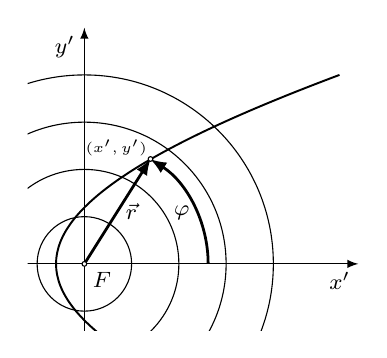
\begin{tikzpicture}[scale=1.2]
        \footnotesize
        \clip (-.3, -0.7) rectangle + (3.5, 3.2);

        \coordinate (xy) at (1, 1.11) {};
        \coordinate (F) at (.3, 0) {};

        \draw [line width = .7pt](3, 2) .. controls (-1, .5) and (-1, -.5) .. (3, -2);

        \draw [-latex] (.3, -2.2) -- (.3, 2.5);
        \draw [-latex] (-1, 0) -- (3.2, 0);

        \draw (F) circle (.5);
        \draw (F) circle (1);
        \draw (F) circle (1.5);
        \draw (F) circle (2);
        \draw (1.61, 0) [-latex, line width=1pt] arc (0:57.8:1.31);
        \draw [-latex, line width=1pt] (.3, 0) -- (1, 1.11);

        \draw (1.05, 1.05) node [anchor=south east] {\tiny{$(x', y')$}};
        \draw (F) node [anchor=north west] {$F$};
        \draw (.65, .55) node [anchor=west] {$\vec r$};
        \draw (1.5, .7) node [anchor=north east] {$\boldsymbol{\varphi}$};
        \draw (3.2, 0) node [anchor=north east] {$x'$};
        \draw (-.1, 2.5) node [anchor=north west] {$y'$};

        \draw (F) [fill=white] circle(.025);
        \draw (xy) [fill=white] circle(.025);
    \end{tikzpicture}
    \caption{}
    \label{pic:parabola-polar-coord}
\end{wrapfigure}
Перенесем теперь фокус параболы в начало координат и получим уравнение параболы в полярных координатах. Для этого нужно сделать такую замену: $x' \hookrightarrow x - p/2$, значит $x \hookrightarrow x' + p/2$, а $y' \hookrightarrow y$. Запишем уравнение параболы в новых координатах:
\begin{gather*}
    y^2 = 2px,\\
    (y')^2 = 2 p \left(x' + \frac{p}{2} \right).
\end{gather*}
Перейдём в полярные координаты в полученном равенстве:
\begin{gather*}
    r^2 \sin^2 \varphi = p^2 + 2pr\cos \varphi,\\
    r^2 \cdot \sin^2 \varphi - r \cdot 2 p  \cos \varphi - p^2,\\
    D = 4p^2 \cos^2 \varphi + 4 p^2 \sin^2 \varphi = 4 p^2,\\
    r = \frac{2p \cos \varphi \pm 2p}{2\sin^2 \varphi}, \quad r \geqslant 0,\\
    r = \frac{p (\cos \varphi + 1)}{1 - \cos^2 \varphi} = \frac{p (\cos \varphi + 1)}{(1 - \cos\varphi)(1 + \cos\varphi)} = \frac{p}{1 - \cos \varphi}.
\end{gather*}
Если же параболу развернуть на $180^\circ$, в знаменателе будет знак плюс. Это завершает вывод уравнения параболы в полярных координатах:
\begin{equation}
    r = \frac{p}{1 \pm \cos \varphi}.
\end{equation}

\begin{wrapfigure}{r}{0.45\tw}
    \centering
    \vspace{-.5pc}
    \tikzsetnextfilename{parabola-optic-property}
    \begin{tikzpicture}[scale=1.2]
        \footnotesize
        \clip (-.4, -1) rectangle + (4, 3.5);

        \coordinate (xy) at (1, 1.11) {};
        \coordinate (F) at (.3, 0) {};

        \draw [line width = .7pt](3, 2) .. controls (-1, .5) and (-1, -.5) .. (3, -2);

        \draw [-latex] (0, -2.2) -- (0, 2.5);
        \draw [-latex] (-1, 0) -- (3.5, 0);

        \draw [-latex, line width=1pt] (F) -- (xy);
        \draw [-latex, line width=1pt] (xy) -- (2, 1.11);
        \draw [-latex, line width=1pt] (xy) -- (2, 1.67);
        \draw (xy) -- (3, 1.11);
        \draw [dashes] (3, 2.21) -- (-.5, 0.29);

        \draw (1.2, 1.11) node [anchor=south east] {$(x, y)$};
        \draw (F) node [anchor=north] {$F$};
        \draw (.65, .55) node [anchor=west] {$\vec r$};
        \draw (1.5, 1.11) node [anchor=north] {$\vec x$};
        \draw (1.5, 1.39) node [anchor=south] {$\vec t$};

        \draw (3.5, 0) node [anchor=north east] {$x$};
        \draw (0, 2.5) node [anchor=north west] {$y$};

        \draw (F) [fill=white] circle(.025);
        \draw (xy) [fill=white] circle(.025);
    \end{tikzpicture}
    \caption{}
    \label{pic:parabola-optic-property}
\end{wrapfigure}
Как и все конические сечения, парабола обладает \imp{оптическим свойством}, которое формулируется таким образом: пучок лучей, параллельных оси параболы, отражаясь в последней, собирается в её фокусе. И наоборот, свет от точечного источника, находящегося в фокусе, отражается параболой в пучок параллельных её оси лучей.

Аналогично доказательству оптического свойства эллипса рассмотрим случай только верхней ветви. Выберем на ней произвольную точку $(x, y)$. Тогда вектор, определяющий направление луча из фокуса в выбранную точку задается вектором $\vec r = (x - p/2, y)$. Направление, соответствующее оси параболы, зададим единичным вектором $\vec x = (1, 0)$, так как ось параболы с каноническим уравнением совпадает с осью абсцисс. Остается найти вектор $\vec t$ касательной в точке $(x, y)$. Для верхней ветви параболы каноническое уравнение эквивалентно $y = \sqrt{2px}$. Найдем производную данной функции:
\begin{gather*}
    y' = \frac{2p}{2\sqrt{2px}} = \sqrt{\frac{p}{2x}}.
\end{gather*}
Значит направляющий вектор касательной можно представить в виде
\begin{equation*}
    \vec t =
    \begin{pmatrix}
        1\\
        y'_x
    \end{pmatrix} =
    \begin{pmatrix}
        1\\
        \sqrt{\dfrac{p}{2x}}
    \end{pmatrix}.
\end{equation*}

Остается проверить равенство косинусов углов между векторами $\vec r$ и $\vec t$ и векторами $\vec x$ и $\vec t$:
\begin{gather*}
    \frac{\scalar{r}{t}}{|\vec r| | \vec t|} = \frac{\scalar{x}{t}}{|\vec x| |\vec t|},\\
    \scalar{r}{t} = |\vec r| \scalar{x}{t},\\
    \left(x - \frac{p}{2}\right)\cdot 1 + y \cdot \sqrt{\frac{p}{2x}}  = \sqrt{\left( x - \frac{p}{2} \right)^2 + y^2 } \left(1 \cdot 1 + 0 \cdot \sqrt{\frac{p}{2x}} \,\right),\\
    \left(x - \frac{p}{2}\right)^2 + \frac{y^2 p}{2x} + 2 y \sqrt{\frac{p}{2x}} \left(x - \frac{p}{2}\right) = \left(x - \frac{p}{2}\right)^2 + y^2,\\
    2  \sqrt{\frac{p}{2x}} \left(x - \frac{p}{2}\right) =  y \left( 1 - \frac{p}{2x} \right),\\
    \sqrt{\frac{4x^2p}{2x}} \left(1 - \frac{p}{2x}\right) =  y \left( 1 - \frac{p}{2x} \right),\\
    \sqrt{2xp}  =  y.
\end{gather*}
Получено уравнение верхней ветви параболы, которому, очевидно, координаты точки, принадлежащей параболе, удовлетворяют. Следовательно, оптическое свойство доказано.

Покажем, что парабола является коническим сечением. Для этого рассмотрим каноническое уравнение конической поверхности
\begin{equation*}
    \frac{x^2}{a^2} + \frac{y^2}{b^2} - \frac{z^2}{c^2} = 0
\end{equation*}
и секущую плоскость, параллельную образующей конуса и задаваемую уравнением
\begin{equation*}
    z = \frac{c(x + d)}{a},
\end{equation*}
где коэффициенты $a, b, c$ определяют вид поверхности, а $d$~--- положение плоскости. Подставим второе в первое:
\begin{gather*}
    \frac{x^2}{a^2} + \frac{y^2}{b^2} = \frac{x^2 + d^2 + 2yd}{a^2},\\
    \frac{y^2}{b^2} = \frac{d^2 + 2xd}{a^2},\\
    y^2 = 2 x \underbrace{\frac{b^2d}{a^2}}_p + \frac{b^2 d^2}{a^2}.
\end{gather*}
С точностью до вертикального сдвига получено каноническое уравнение параболы, что подтверждает принадлежность параболы множеству конических сечений.


\subsection{Гипербола}

	\section{Астрофизика}
\subsection{Звёздные величины}
Звёздная величина~--- безразмерная числовая характеристика яркости объекта. Принято, что увеличению светового потока в 100 раз соответствует уменьшение звёздной величины ровно на 5 единиц. Тогда уменьшение звёздной величины на одну единицу означает увеличение плотности светового потока в $\sqrt[5]{100}\approx 2.512$~раз, то есть звёздные величины являются логарифмической шкалой измерения плотности потока. Зависимость, связывающая отношение освещённостей $E_1$ и $E_2$ и разность звёздных величин $m_1$ и $m_2$ двух объектов, называется \term{формулой Погсона} и имеет вид
\begin{equation}
    \frac{E_1}{E_2} = 10^{0.4(m_2 - m_1)} \quad \text{или} \quad m_2 = m_1 + 2.5 \lg \frac{E_1}{E_2}.
    \label{eq:pogson-law}
\end{equation}

Широко используется понятие \term{абсолютной звёздной величины} $M$~--- это звёздная величина при наблюдении с установленного расстояния~$R_0$: для звёзд и объектов вне Солнечной системы~---~10~пк, для тел Солнечной системы~---~1~\au, причем считается, что тело находится в 1~\au~и от наблюдателя и от Солнца, а фаза равна единице, то есть можно считать, что наблюдатель находится в центре Солнца, а~тело~--- в~1~\au~от него.

Абсолютную звёздную величину объекта вне Солнечной системы можно получить по формуле Погсона \eqref{eq:pogson-law} из наблюдаемой звёздной величины~$m$ и расстояния~$r$ до него
\begin{equation}
    M = m + 2.5 \lg \frac{E}{E_\text{абс}} = m + 2.5 \lg \frac{L \cdot R_0^2}{r^2 \cdot L} = m + 5 \lg \frac{R_0}{r}.
    \label{eq:absolute-magnutude}
\end{equation}
Если принимать к рассмотрению межзвездное поглощение~$A$, то формулу  \eqref{eq:absolute-magnutude} необходимо уточнить:
\begin{equation}
    M = m + 5 \lg \frac{R_0}{r} - Ar.
\end{equation}

Важно определить понятие \term{болометрической звёздной величины}~$m_\text{bol}$~--- это звёздная величина, при расчёте которой учитывается полная мощность излучения источника во всем диапазоне длин электромагнитных волн.

Резолюция B2, принятая на Генеральной Асамблеи Международного астрономического союза в 2015 году\,\cite{bolometric-magnitude}, определяет нуль-пункт звёздных величин. Так \imp{абсолютную болометрическую звёздную величину}, равную $0^m$ имеет изотропный источник излучения с мощностью $L_0 = 3.0128 \cdot 10^{28}$~Вт. Данное значение выбрано таким образом, чтобы абсолютная болометрическая звёздная величина Солнца $M_{\text{Bol}\odot}$ составляла $4.74^m$. Такому источнику излучения соответствует наблюдаемая плотность потока
\begin{equation}
    E_0 = \frac{L_0}{4\pi R_0^2} = 2.518021002\ldots \cdot 10^{-8}~\frac{\text{Вт}}{\text{м}^2}.
\end{equation}
Исходя из этого, используя \imp{формулу Погсона}, можно определить болометрическую звёздную величину любого изотропного источника излучения, зная его светимость и расстояние до него.

\term{Фотометрическая звёздная величина}~--- звёздная величина источника в некотором фильтре $\xi$, для которого определена функция чувствительности приемника $S_\xi(\lambda): [0, +\infty] \rightarrow [0,1]$. Определяется выражением
\begin{equation}
    m_\xi = -2.5\lg \frac{\int E(\lambda) S_\xi(\lambda) \, d \lambda}{E_0} + C_\xi,
\end{equation}
где $E(\lambda)$~--- плотность потока излучения от источника на длине волны~$\lambda$, а $C_\xi$~--- нормировочная константа фильтра $\xi$. Несмотря на то, что интегралы определенные, звёздная величина в том или ином фильтре определяется с точностью до нормировки на определенный нуль-пункт.

\begin{wraptable}[15]{r}{0.43\tw}
    \vspace{-0.75pc}
    \footnotesize
    \centering
    \renewcommand{\arraystretch}{1.2}
    \begin{tabular}{|c|c|c|}
        \hline
        Фильтр & $\langle\lambda\rangle$, нм & FWHM, нм \\
        \hline
        $U$    & 365                         & 66       \\
        $B$    & 445                         & 94       \\
        $V$    & 551                         & 88       \\
        $R$    & 658                         & 138      \\
        $I$    & 806                         & 149      \\
        $Y$    & 1020                        & 120      \\
        $J$    & 1220                        & 213      \\
        $H$    & 1630                        & 307      \\
        $K$    & 2190                        & 390      \\
        $L$    & 3450                        & 472      \\
        $M$    & 4750                        & 460      \\
        $N$    & 10500                       & 2500     \\
        \hline
    \end{tabular}
    \caption{Параметры фильтров фотометрической системы Джонсона}
    \label{tbl:johnson-bands}
\end{wraptable}
Для стандартизации фотометрических звёздных величин описаны различные фотометрические системы, особенно распространена система, опубликованная в 1966 году\,\cite{johnson-photometry}, где авторы определяют 8 широкополосных фильтров $U\!BV\!RIJKL$ (позднее были добавлены фильтры $M$ и $N$), параметры которых приведены в Таблице\,\ref{tbl:johnson-bands}, а профили пропускания представлены на \picRef{pic:johnson-bands}. Нуль-пунктом отсчета звездной величины в каждом из фильтров является блеск звезды спектрального класса $A0V$~--- Веги ($\alpha$\,Lyr), которой принимается равным $0.03^m$ в каждом из фильтров.

\begin{figure}[t]
    \centering
    \begin{subcaptionblock}{\tw}
        \centering
        \tikzsetnextfilename{johnson-bands-1}
        \begin{tikzpicture}
            \begin{axis} [
                width   =    \tw,
                height  =    3.5cm,
                xmax    =    1500,
                xmin    =    300,
                xlabel  =    {Длина волны $\lambda$,~нм},
                ylabel  =    {$S_\xi(\lambda)$}
            ]
                \addplot[black, smooth] table[x=l, y=U] {data/filters-data-U.txt} node at (axis cs:350, 0.5) {\scriptsize{$U$}};
                \addplot[black, smooth] table[x=l, y=B] {data/filters-data-B.txt} node at (axis cs:440, 0.5) {\scriptsize{$B$}};
                \addplot[black, smooth] table[x=l, y=V] {data/filters-data-V.txt} node at (axis cs:550, 0.5) {\scriptsize{$V$}};
                \addplot[black, smooth] table[x=l, y=R] {data/filters-data-R.txt} node at (axis cs:700, 0.5) {\scriptsize{$R$}};
                \addplot[black, smooth] table[x=l, y=I] {data/filters-data-I.txt} node at (axis cs:870, 0.5) {\scriptsize{$I$}};
                \addplot[black, smooth] table[x=l, y=J] {data/filters-data-J.txt} node at (axis cs:1250, 0.5) {\scriptsize{$J$}};
            \end{axis}
        \end{tikzpicture}
    \end{subcaptionblock}
    
    \vspace{0.5pc}
    \begin{subcaptionblock}{\tw}
        \centering
        \tikzsetnextfilename{johnson-bands-2}
        \begin{tikzpicture}
            \begin{axis} [
                width   =    \tw,
                height  =    3.5cm,
                xmax    =    15,
                xmin    =    1,
                xlabel  =    {Длина волны $\lambda$,~мкм},
                ylabel  =    {$S_\xi(\lambda)$}
            ]
                \addplot[black, smooth] table[x=l, y=K] {data/filters-data-K.txt} node at (axis cs:2.2, 0.5) {\scriptsize{$K$}};
                \addplot[black, smooth] table[x=l, y=L] {data/filters-data-L.txt} node at (axis cs:3.5, 0.5) {\scriptsize{$L$}};
                \addplot[black, smooth] table[x=l, y=M] {data/filters-data-M.txt} node at (axis cs:5, 0.5) {\scriptsize{$M$}};
                \addplot[black, smooth] table[x=l, y=N] {data/filters-data-N.txt} node at (axis cs:10, 0.5) {\scriptsize{$N$}};
            \end{axis}
        \end{tikzpicture}
    \end{subcaptionblock}
    \caption{Профили пропускания фотометрических фильтров системы $U\!BV\!RIJKLMN$}
    \label{pic:johnson-bands}
\end{figure}

Важно отметить, когда речь идёт звёздной величине без какой-либо кон\-кретизации, обычно имеется в виду видимая звёздная величина, другими словами~--- звёздная величина в фильтре~$V$, и обозначается как~$m_V$ или просто~$m$.

Разность между болометрической и фотометрической звёздными величинами называется \term{болометрической поправкой} (B.C.), которая отличается для разных спектральных классов звёзд и разных фильтров. Болометрическая поправка для фильтра $\xi$ может быть найдена из определения по формуле
\begin{equation}
    \text{B.C.}_\xi = M_\text{Bol} - M_\xi = m_\text{Bol} - m_\xi = 2.5\lg \frac{\int E(\lambda) S_\xi(\lambda) \, d \lambda}{\int E(\lambda)\, d \lambda} + C_\xi - C_\text{Bol},
\end{equation}
где $C_\text{Bol}=0$, если $C_\xi$ была определена с использованием стандарта~$E_0$.


\subsection{Закон Стефана-Больцмана}
\term{Закон Стефана~--- Больцмана} определяет зависимость плотности мощности излучения абсолютно чёрного тела (АЧТ) $u$ от его температуры $T$:
\begin{equation}
	u = a T^4,
\end{equation}
где $a$~--- некая универсальная константа.
Отсюда полная светимость АЧТ с площадью поверхности $S$
\begin{equation}
	L = S \sigma T^4,
	\label{eq:steff-bol-law}
\end{equation}
константа $\sigma$ называется \term{постоянной Стефана-Больцмана}.

Важно отметить, что \imp{закон Стефана-Больцмана}~--- прямое следствие формулы Планка (\ref{eq:plancks-law-nu} -- \ref{eq:plancks-law-lambda}), так как, исходя из физического смысла формулы Планка, справедливы равенства
\begin{multline}
	\sigma T^4 = \int\limits^\infty_0 B(\lambda, T) \,d \lambda \int\limits_0^{\pi/2} \sin \varphi \,d \varphi \int\limits_0^{2\pi} \cos \varphi \,d \theta = \pi \int\limits^\infty_0 B(\lambda, T) \,d \lambda =\\
	= \int\limits^\infty_0 B(\nu, T) \,d \nu \int\limits_0^{\pi/2} \sin \varphi \,d varphi \int\limits_0^{2\pi} \cos \varphi \,d theta = \pi \int\limits^\infty_0 B(\nu, T) \,d \nu.
\end{multline}

Здесь интегрирование ведется в сферических координатах $(\varphi, \theta)$ по телесному углу $d\Omega = d\varphi \cos \varphi d\theta$. А $\sin \varphi$ во втором интеграле отвечает за проекцию единичной площадки на направление излучения. Вычислим данный интеграл, чтобы получить значение постоянной Стефана-Больцмана:
\begin{equation*}
	\sigma T^4 = \pi \int\limits_0^{\infty} \frac{2h\nu^3}{c^2}\cdot \frac{1}{\exp\left(\frac{h\nu}{kT}\right)-1} \,d \nu.
\end{equation*}
Сделаем замену $x = \frac{h \nu}{k T}$, так как $dx = \frac{h}{k T} d\nu$, то
\begin{equation*}
	\sigma T^4 = \frac{2\pi}{c^2}  \int\limits_0^{\infty} \underbrace{\frac{k^3 T^3}{h^2} x^3}_{h\nu^3} \cdot \frac{1}{e^x - 1} \cdot \underbrace{\frac{kT}{h} \,d x}_{d\nu} = \frac{2 \pi k^4 T^4}{c^2 h^3} \int\limits_0^{\infty} \frac{x^3 \,d x}{e^x - 1}.
\end{equation*}
Значение табличного интеграла $\int\limits_0^{\infty} \frac{x^3 \,d x}{e^x - 1}$ равно $\frac{\pi^4}{15}$, откуда
\begin{equation*}
	\sigma = \frac{2 \pi^5 k^4}{15 c^2 h^3} = 5.67 \cdot 10^{-8}~\frac{\text{Вт}}{\text{м}^2 \cdot \text{К}^4}.
\end{equation*}

Для звёзд главной последовательности выполняется соотношение $L \sim M^{\alpha}$, где~$\alpha$~--- коэффициент пропорциональности, который зависит от массы звезды следующим образом:
\begin{align*}
	\alpha &= 2.5,\quad M < 0.5 M_\odot; \\
	\alpha &= 4, \quad 0.5 M_\odot < M < 8 M_\odot;\\
	\alpha &= 2.5, \quad  M > 8 M_\odot.
	%\alpha &= 1, \quad M > 20 M_\odot.
\end{align*}
Также существует примерная зависимость светимости звёзды от её радиуса, имеющая вид  $L\sim R^{5.2}$.

\subsection{Энергия излучения}
\term{Энергия излучения}~--- энергия, переносимая излучением ($Q_e$).\\
\term{Поток излучения}~--- физическая величина, характеризующая мощность, переносимую излучением,
\begin{equation}
	\Phi_e = \frac{d Q_e}{dt}.
\end{equation}
\imp{Теорема Гаусса}: через любую замкнутую поверхность потоки от одинаковых источников равны.

\term{Спектральная плотность потока излучения}~--- поток излучения, приходящийся на малый единичный интервал спектра,
\begin{equation}
	\Phi_{e, \lambda}(\lambda) = \frac{d\Phi_e(\lambda)}{d\lambda}, \quad\quad \Phi_{e, \nu}(\nu) = \frac{d\Phi_e(\nu)}{d\nu} =  \frac{\lambda^2}{c}\Phi_{e, \lambda}(\lambda).
\end{equation}

\term{Объемная плотность энергии излучения}~--- количество энергии на единицу объема
\begin{equation}
	U_e = \frac{d Q_e}{dV}.
\end{equation}

\term{Светимость}~--- величина, представляющая собой световой поток излучения, испускаемого с малого участка светящейся поверхности единичной площади,
\begin{equation}
	M_e = \frac{d \Phi_e}{dS_1},
\end{equation}
здесь $S_1$~--- площадь объекта, испускающего энергию.

\term{Яркость}~--- световой поток, приходящийся на единичный телесный угол, в расчёте на единичную площадку проекции излучающей поверхности на картинную плоскость,
\begin{equation}
	L_e = \frac{d^2 \Phi_e}{d \Omega\,dS_1 \cos \varepsilon},
\end{equation}
где $\varepsilon$~--- угол между направлением потока излучения и нормалью к плоскости излучающей поверхности.

\term{Интегральная яркость}~--- интеграл яркости по видимой поверхности источника. Показывает количество энергии, пришедшее от источника за единицу времени.
\begin{equation}
	\Lambda_e = \int \limits_S L_e(\vec{r})\,ds.
\end{equation}
\term{Освещенность}~--- величина, равная отношению светового потока, падающего на малый участок поверхности, к его площади~--- поверхностная плотность потока
\begin{equation}
	E_e = \frac{d\Phi_e}{dS_2} \sim \frac{1}{r^2},
\end{equation}
здесь $S_2$~--- площадь поверхности приёмника, $r$~--- расстояние от источника.

\subsection{Альбедо}
\term{Альбедо}~($A$)~--- характеристика отражательной способности поверхности какого-либо объекта. Альбедо является отношением отражённого светового потока к падающему на поверхность объекта. Тогда для нахождения поглощённой части излучения используется соотношение
\begin{equation}
    E_\text{п} = E_0 \cdot (1-A),
\end{equation}
где $E_{\text{п}}$~--- поглощённая часть излучения, $E_0$~--- пришедшее излучение, $A$~--- альбедо. А для отражённой части излучения $E_{\text{отр}}$ можно использовать формулу
\begin{equation}
    E_{\text{отр}}= A \cdot E_0.
\end{equation}

Существует несколько видов альбедо: \imp{геометрическое}, \imp{сферическое} и \imp{бондовское}. \term{Геометрическое альбедо} равно отношению освещённости у Земли, создаваемой планетой в полной фазе, к освещённости, которую создал бы плоский абсолютно белый экран того же размера, что и планета, расположенный на её месте перпендикулярно лучу зрения и солнечным лучам. \term{Сферическое альбедо} определяется как отношение светового потока, рассеянного телом во всех направлениях, к потоку, падающему на это тело. Может быть определено как для некоторого диапазона длин волн, так и для всего спектра. Сферическое альбедо для всего спектра излучения называется \term{альбедо Бонда}.

\subsection{Энергия и импульс фотона}
\term{Фотон}~--- материальная, электрически нейтральная частица, квант электромагнитного поля (переносчик электромагнитного взаимодействия). В силу корпускулярно-волнового дуализма, фотон можно рассматривать либо как частицу, либо как волну. Фотон не имеет массы, однако обладает энергией
\begin{equation}
	E = h \nu = \frac{h c}{\lambda}
\end{equation}
и импульсом, определяемым как
\begin{equation}
	p = \frac{E}{c} = \frac{h}{\lambda},
\end{equation}
где коэффициент пропорциональности $h = 6.63 \times 10^{-34}~\text{Дж}\cdot\text{с}$ называется \imp{постоянной Планка}.

\subsection{Линии излучения и поглощения}

\textbf{Планетарная модель атома (Резерфорда)} описывает модель атома, состоящего из маленького ядра, в котором сосредоточена почти вся масса атома, и электронов, обращающихся по круговым орбитам вокргу ядра. \\

\textbf{Модель атома Бора} содержит в основе модель атома Резерфорда, но в данной модели электроны могут обращаться только по строго определённым орбитам.\\

\textbf{Певый постулат Бора.} Электроны в атоме могут двигаться только по определенным (стационарным) орбитам, находясь на которых они не излучают энергию.  Причём, стационарными являются лишь те орбиты, при движении по которым момент количества движения электрона равен целому числу постоянных Планка:

\begin{equation}
	m_e v r_n = \frac{n h}{2 \pi} = n \hbar,~n \in \mathbb{N} \backslash \lbrace 0 \rbrace
\end{equation}
где $m_e$~--- масса электрона, $v$~--- скорость электрона, $r_n$~--- радиус $n$-ой орбиты, $h$~--- постоянная Планка.

Рассмотрим электрон, находящийся на произвольной орбите вокруг ядра некоторого атома. Запишем для него равенство центробежной и Кулоновской силы.

\begin{equation}
	\frac{m_e v^2}{r_n} = \frac{Z^2 e^2}{4 \pi \varepsilon_0 r_n^2},
\end{equation}
где $Z$~--- зарядовое число, $e$~--- заряд электрона, $\varepsilon_0$~--- электрическая постоянная.

Из данного уравнения и первого постулата Бора можно получить значени для радиуса $n$-ой орбиты:

\begin{equation}
	r_n = \frac{\varepsilon_0 n^2 h^2}{\pi m_e Z^2 e^2}.
\end{equation}
Отсюда можно получить значение боровского радиуса~--- радиус первой орбиты для атома водорода $(Z = 1,~n = 1)$. $a_0 \approx 5,291769241 \times 10^{-11}~text{м}$. \\

Считая, что полная энергия электроа равна кинетической, взятой со знаком минус, можно получить выражение для полной энергии электрона на некоторой орбите:

\begin{equation}
	E_n = -\frac{m_e Z^2 e^2}{8 n^2 h^2 \varepsilon_0}.
\end{equation}

Посчитаем, как изменяется энергия эектрона при переходе с уровня $n$ на уровень $m$:
\begin{equation}
	\Delta E_{n, m} = \frac{m_e Z^2 e^2}{8 n^2 h^2 \varepsilon_0} \left( \frac{1}{n^2} - \frac{1}{m^2}\right) = h \nu.
\end{equation}
Получается, что при переходе с нижнего уровня на верхний может поглотиться фотон с определенной частотой, а при ообратном переходе~--- излучиться. Частоту фотона можно найти из следущего выражения:
\begin{equation}
	\nu_{n, m} =
	\frac{\Delta E_{n, m}}{h} = \frac{m_e Z^2 e^2}{8 n^2 h^3 \varepsilon_0} \left( \frac{1}{n^2} - \frac{1}{m^2}\right) = R Z^2 \left(\frac{1}{n^2} - \frac{1}{m^2} \right),
\end{equation}
где $R$~--- постоянная Ридберга $(10973731~\text{м}^{-1})$.

Из-за того, что энергетических уровней в атоме лишь счетное число, то и возможные длины частот поглощения и излучения принимают только счетное количество значений.

\subsection{Формула Планка}
\label{sec:planck-law}
\term{Формула Планка}~--- выражение для спектральной плотности мощности излучения
 абсолютно чёрного тела на интервале частот $[\nu, \nu + d \nu)$,
 распространяющегося в телесном угле $d\Omega$, которое было получено Максом
 Планком в 1900~году. Данное выражение имеет следующий вид:
\begin{equation}
	B_\nu(\nu,T) 
	= \frac{2h\nu^3}{c^2}\cdot \frac{1}{\exp\left(\frac{h\nu}{kT}\right)-1} 
	= \left[ \frac{\text{Вт}}{\text{м}^2 \cdot \text{Гц} \cdot \text{ср}}\right],
	\label{eq:plancks-law-nu}
\end{equation}
где $\nu$~--- частота излучения, $T$~--- температура АЧТ, $h$~--- постоянная
 Планка, $k$~--- постоянная Больцмана, $c$~--- скорость света. Если записать закон
 излучения Планка \eqref{eq:plancks-law-nu} для длин волн, получится
\begin{equation}
	B_\lambda(\lambda,T)
	= \frac{2hc^2}{\lambda^5} \cdot \frac{1}{\exp\left(\frac{hc}{\lambda kT}\right)-1} 
	= \left[ \frac{\text{Вт}}{\text{м}^3 \cdot \text{ср}}\right].
	\label{eq:plancks-law-lambda}
\end{equation}

Стоит заметить, что при переходе к выражению формулы Планка через длину
 волны также меняется выражение для интервала, поэтому в результате 
 изменяется степень переменной в знаменателе.

Формула Планка появилась, когда стало ясно, что формула Рэлея-Джинса
 удовлетворительно описывает излучение только в области больших длин волн,
 а~с~убыванием длин волн сильно расходится с реальными данными. Однако формулу
 Рэлея-Джинса используют и сейчас для описания спектра абсолютно чёрного тела 
 в длинноволновой области.


Проделаем обратные действия: получим формулу Рэлея-Джинса из формулы Планка. Длинноволновая часть спектра характеризуется соотношением $h\nu \ll kT$, то есть
\begin{equation*}
	\exp\left( \frac{h\nu}{kT}\right) \approx 1 + \frac{h\nu}{kT}.
\end{equation*}
Подставляя данное выражение в знаменатель \eqref{eq:plancks-law-nu}, получим
\begin{equation*}
	B_\nu(\nu,T) 
	\approx \frac{2h\nu^3}{c^2}\cdot \frac{1}{1 + \frac{h\nu}{kT} - 1} 
	= \frac{2h\nu^3 }{c^2}\cdot \frac{k T}{ h \nu} 
	= \frac{2 \nu^2 k T}{c^2}.
\end{equation*}

\begin{figure}[t]
	\centering
	\vspace{-.9pc}
	\begin{tikzpicture}
		\begin{axis}[
			width 	=	\tw,
			height	=	8cm,
			ymax	=	1e+14,
			xmax	=	2000,
			xmin	=	0,
			ymin	=	0,
			xlabel	=	{Длина волны $\lambda$,~нм},
			ylabel 	= 	{$B_\lambda(\lambda, T)$,~$\text{Вт} \cdot \text{м}^{-3}$},
			restrict y to domain		=	0:1e+15
			]
			\addplot+[dashed, thin, black] table[x=l, y=tl] {data/planck.txt};
			\addplot[black] table[x=l, y=t3800] {data/planck.txt} node at (axis cs:870, 1.4e+13) {\scriptsize{$3800$~K}};
			\addplot+[black, smooth, solid] table[x=l, y=t4500] {data/planck.txt} node at (axis cs:750, 2.7e+13) {\scriptsize{$4500$~K}};
			\addplot+[black, smooth, solid] table[x=l, y=t5000] {data/planck.txt}node at (axis cs:710, 4.4e+13) {\scriptsize{$5000$~K}};
			\addplot+[black, smooth, solid] table[x=l, y=t5800] {data/planck.txt}node at (axis cs:640, 8.7e+13) {\scriptsize{$5800$~K}};
			\addplot+[black, smooth, solid] table[x=l, y=t7000] {data/planck.txt}node at (axis cs:1340, 3.3e+13) {\scriptsize{$7000$~K}};
			\addplot+[black, smooth, solid] table[x=l, y=t10000] {data/planck.txt} node at (axis cs:1430, 5.5e+13) {\scriptsize{$10000$~K}};
			\addplot+[black, smooth, solid] table[x=l, y=t20000] {data/planck.txt} node at (axis cs:1670, 8.0e+13) {\scriptsize{$20000$~K}};
		\end{axis}
	\end{tikzpicture}
	\caption{Кривые спектральной плотности мощности изотропного излучения АЧТ с разной температурой}
	\label{pic:wien-law}
\end{figure}

Проделав те же действия для формулы Планка через длину волны, получим:
\begin{equation}
	B(\lambda, T) 
	\simeq \frac{2 c k T}{\lambda^4}, \quad\quad B(\nu, T) \simeq \frac{2 \nu^2 k T}{c^2}.
	\label{Ray-Jean}
\end{equation}

В коротковолновой области, наоборот, $h \nu \gg kT$, следовательно, единица в знаменателе формулы Планка много меньше стоящей там экспоненты, то есть
\begin{equation*}
	\frac{1}{\exp\left(\frac{h\nu}{kT}\right)-1} 
	\approx \frac{1}{\exp\left(\frac{h\nu}{kT}\right)} 
	= \exp\left(-\frac{h\nu}{kT}\right).
\end{equation*}
Отсюда получаются приближения, называемые приближениями Вина:
\begin{equation}
	B ( \lambda, T) 
	\simeq \frac{2 h c^2}{\lambda^5} \exp\left(-\frac{h c}{\lambda k T}\right), \quad B( \nu, T ) 
	\simeq \frac{2 h \nu^3}{c^2} \exp\left(-\frac{h \nu}{k T}\right).
\end{equation}

\subsection{Количество фотонов. Средняя Энергия}
Если разделить формулу Планка на энергию одного фотона, то можно получить функцию распределения количества фотонов по энергиям
\begin{equation*}
	\frac{\pi B_{\lambda}}{E_{\gamma}} = \frac{2 \pi c}{\lambda^4} \cdot \frac{1}{\exp\left(\frac{hc}{\lambda k T}\right)-1} = f_{\lambda}
\end{equation*}
Интегрируя от 0 до $\infty$ можно получить полное количество фотонов излучаемое АЧТ:
\begin{equation*}
	N = \int_{0}^{\infty}{\pi f_{\lambda}d\lambda} = \int_{0}^{\infty}{\frac{2\pi c}{\lambda^4} \cdot \frac{d\lambda}{\exp\left(\frac{hc}{\lambda k T}\right)-1}}
\end{equation*}
Сделав замену $x = \frac{hc}{\lambda kt}$ интеграл сводится к
\begin{equation*}
	N = \frac{2\pi k^3 T^3}{h^3 c^2}\int_{0}^{\infty}{\frac{x^2 dx}{e^x-1}}
\end{equation*}
Последний интеграл вычисляется аналочично интегралу, что появляется при выводе закона Стефана-Больцмана и равен $2\zeta(3)$, отсюда
\begin{equation}
	N = \frac{4\pi k^3 \zeta(3)}{h^3 c^2} \cdot T^3 = \beta T^3
\end{equation}
Константа пропорциональности $\beta$ равна примерно $1.52 \cdot 10^{15}$. Если поделить полную энергию излучаемое АЧТ на полное количество фотонов, то можно получить \term{среднюю энергию чернотельного фотона}:
\begin{equation}
	\overline{E_{\gamma}} = \frac{\sigma T^4}{\beta T^3} \simeq 2.7 k T
\end{equation}
\subsection{Закон смещения Вина}
\textit{Закон смещения Виина} --- закон, устанавливающий зависимость длины волны от температуры чёрного тела, на которой поток излучения энергии чёрного тела достигает своего максимума (Рис.\ref{pic:wien-law}).

\begin{figure}[h!]
\begin{center}
\includegraphics[scale=0.35]{Wien-law}
\end{center}
\caption{Кривые потока излучения абсолютно чёрных тел с разной температурой}\label{pic:wien-law}
\end{figure}

Длину волны, на которой интенсивность излучения абсолютно чёрного тела достигает своего максимума, можно определить по следующей формуле:
\begin{equation}
\lambda_{max}\approx\frac{b}{T}
\end{equation}

Где $b$ --- постоянная Вина равная $b\approx0.0029 $ $\text{м} \cdot \text{К}$

Данная формула получается путём нахождения экстремума \textit{закона излучения Планка} для абсолютно чёрного тела, записанного для длин волн:
\begin{equation}
B(\lambda,T)=\frac{2hc}{\lambda^5 e^{hc/\lambda KT}-1}
\end{equation}

\subsection{Эффект Доплера. Красное смещение}
\term{Эффект Доплера}~--- эффект изменения частоты и длины волны электромагнитного излучения, регистрируемого приёмником, вызванный относительным движением источника и приёмника (\lookPicRef{doppler-ef}).

При $\Delta \lambda \ll \lambda_0$ с большой точностью выполняется следующее важное соотношение:
\begin{equation}
    \beta \equiv \dfrac{v}{c} = \dfrac{\lambda - \lambda_0}{\lambda_0} \equiv \dfrac{\Delta \lambda}{\lambda_0},
    \label{eq:dopler-ef-simple}
\end{equation}
\begin{wrapfigure}[6]{r}{0.5\tw}
    \centering
    \vspace{-.5pc}
    \tikzsetnextfilename{doppler-effect}
    \begin{tikzpicture}
        \clip (-1.5,-0.8) rectangle + (5.5, 1.6);
        \foreach \i in {12,...,0} {
            \pgfmathsetmacro\m{int(mod(\i * 5, 2))};
            \ifthenelse{\m = 0}{
                \fill [lightgray] ($({(\i / 8)}, 0)$) circle ({0.5*5/12*\i});
            }{
                \fill [white] ($({(\i / 8)}, 0)$) circle ({0.5*5/12*\i});
            };
        };
        \filldraw (0, 0) circle (0.05);
        \draw [-latex, line width=1pt] (-1.1, 0) -- (-1.5, 0);
        \begin{axis}[
            xmin    =   -1,
            xmax    =   4,
            ymin    =   -1,
            ymax    =   1,
            width   =   6.6cm,
            height  =   3.6cm,
            xshift  =   -1cm,
            yshift  =   -1cm,
            grid    =   none,
            ticks   =   none,
            axis line style = {draw=none},
            tick style = {draw=none},
        ]
            \addplot+[domain=-1:0, samples=1000, smooth, black, line width = 1pt]{0.6*sin(deg(37.7*x))};
            \addplot+[domain=0:4, samples=200, black, line width = 1pt]{0.6*sin(deg(37.7/4*x))};
        \end{axis}
    \end{tikzpicture}
    \caption{Эффект Доплера}
    \label{doppler-ef}
\end{wrapfigure}
где $\lambda_0$~--- лабораторная длина волны излучения источника, а $\lambda$~--- наблюдаемая. В действительности же имеет место более общий случай: \imp{релятивистский эффект Доплера}, обусловленный проявлением СТО при $v \simeq c$, для которого формула~\eqref{eq:dopler-ef-simple} усложняется и принимает вид
\begin{equation}
\nu = \nu_0 \cdot \dfrac{\sqrt{1 - \beta^2}}{1 + \beta \cdot \cos\theta},
\label{eq:dopler-ef-rel}
\end{equation}
где $\nu$~--- частота, с которой наблюдатель принимает волны, $\nu_0$~--- частота, с которой источник испускает волны, $v$~--- скорость источника, $\theta$~--- угол между направлением на источник и вектором его скорости в системе отсчёта приёмника. Если источник радиально удаляется от наблюдателя, то $\theta = 0$, если приближается, то $\theta =\pi$. Важно, что~\eqref{eq:dopler-ef-simple} напрямую следует из \eqref{eq:dopler-ef-rel} при $\beta  \ll 1$.

\term{Красное смещение}~--- явление сдвига спектральных линий химических элементов в красную (длинноволновую) сторону, обусловленное относительным движение объектов. Параметр красного смещения определяется из наблюдаемой и лабораторной длин волн как
\begin{equation}
z = \dfrac{\lambda - \lambda_0}{\lambda_0}.
\end{equation}

Доплеровское смещение длины волны в спектре источника, движущегося с лучевой скоростью $v_{r}$ и полной скоростью $v$,
\begin{equation}
z = \dfrac{1 + v_r / c}{\sqrt{1 - \beta^2}}.
\end{equation}

\term{Гравитационное красное смещение}~--- проявление эффекта изменения частоты излучения, испущенного массивным объектом, таким как звезда или чёрная дыра. Наблюдается как сдвиг спектральных линий в спектре источника в красную область спектра. Гравитационное красное смещение определяется из формулы, выведенной Эйнштейном,
\begin{equation}
z_G=\dfrac{GM}{c^2 R}-\dfrac{GM}{c^2 r},
\label{eq:grav-red-shift}
\end{equation}
где $M$~--- масса гравитирующего тела, $R$~--- радиальное расстояние от центра масс тела до точки излучения (радиус источника), $r$~---  радиальное расстояние от центра масс источника до точки наблюдения. В случае, когда наблюдатель находится от источника много дальше его радиуса, т.\,е. выполняется соотношение $r \gg R$, выражение~\eqref{eq:grav-red-shift} можно упростить до
\begin{equation}
z_G \simeq \dfrac{GM}{c^2 R}.
\end{equation}

\subsection{Давление излучения}
\term{Давление электромагнитного излучения}, падающего на поверхность тела, в отсутствии рассеяния выражается формулой
\begin{equation}
	p = \frac{I}{c} \cdot (1 - k + A) \cdot \cos \beta,
\end{equation}
здесь $I$~--- поток падающего излучения, $c$~--- скорость света, $k$~--- коэффициент пропускания, $A$~--- коэффициент отражения, а $\beta$~--- угол падения излучения.

\term{Давление фотонного газа} определяется соотношением
\begin{equation}
	p_\text{ф.г.} = \frac{u}{3} = \frac{4 \sigma T^4}{3c},
\end{equation}
где $u$~--- плотность энергии фотонного газа, $T$~--- температура фотонного газа.

Возможными областями применения являются солнечный парус, а в отдалённом будущем~--- фотонный двигатель.

\subsection{Предел Эддингтона}
\term{Предел Эддингтона}~--- величина мощности электромагнитного излучения, исходящего из недр звезды, при которой его давления достаточно для компенсации веса оболочек звезды, которые окружают зону термоядерных реакций, то есть звезда находится в состоянии равновесия: не сжимается и не расширяется.\\
Сила тяжести $F_g$, действующая со стороны тела массы $M$ на протон, находящийся на расстоянии $r$ от него, равна
\begin{equation}
    F_g = \frac{G M m_p}{r^2}.
\end{equation}
Поток излучения $I$  от тела со светимостью $L$ на расстоянии $r$ выражается выражается, как
\begin{equation}
    I=\frac{L}{4\pi r^2}.
\end{equation}
Тогда сила $F_r$, действующая на электрон вследствие томсоновского рассеяния фотонов на электронах,
\begin{equation}
    F_r = \frac{I \sigma_T}{c},
\end{equation}
где $\sigma_T$~--- томсоновское сечение рассеяния фотона на электроне, равное
\begin{equation}
    \sigma_T = \left(\frac{8\pi}{3}\right)\left(\frac{e^2}{m_e c^2}\right)^2 = 6.65 \times 10^{-29}~\text{м}^2.
\end{equation}
Таким образом, так как $F_g = F_r$, то
\begin{equation}
    L_\text{Эдд} = \frac{4\pi G M m_p c}{\sigma_T} =  \frac{M}{M_\odot} \times 10^{31}~\text{Вт}.
\end{equation}

\subsection{Гравитационное линзирование}

\textit{Гравитационная линза} --- массивное тело или система тел (галактик, скопление галактик, скопление тёмной материи), искривляющая своим гравитационным полем направление распространения электромагнитного излучения.

На (Рис.\ref{grav-lens}) показано, как происходит гравитационное линзирование. S --- источник электромагнитных волн, O --- наблюдатель, $J_1$ и $J_2$ --- видимые положения источника, $M$ --- массивное тело.

\begin{figure}[h!]
\begin{center}
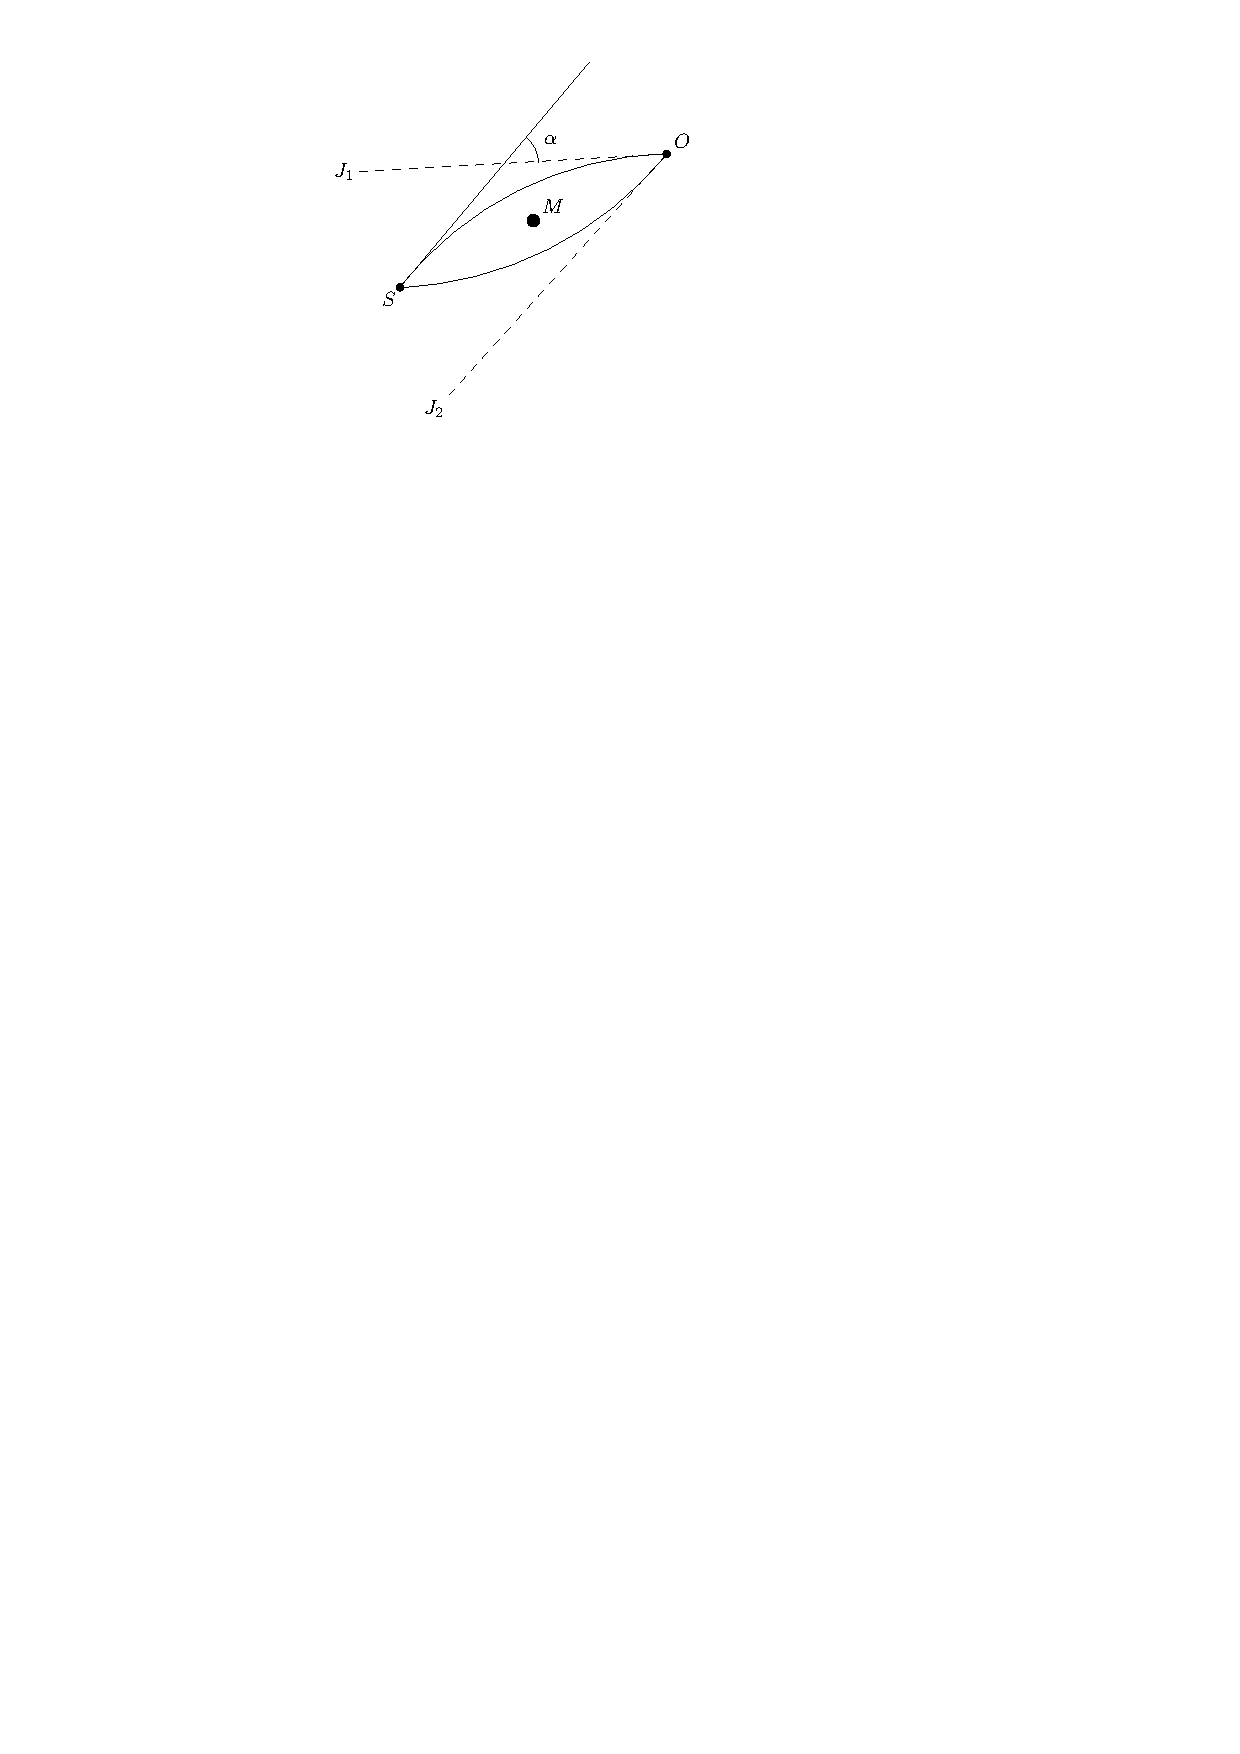
\includegraphics[width=0.4\textwidth]{grav-lens}
\caption{Гравитационное линзирование}\label{grav-lens}
\end{center}
\end{figure}

Найти угол отклонения луча в радианах можно по следующей формуле:
\begin{equation}
\alpha=\frac{4GM}{Rc^2},
\end{equation}
где $M$ --- масса тела, отклоняющего луч, $R$ --- радиус этого тела, $c$ --- скорость света.
\subsection{Шкала электромагнитных волн}

\term{Гамма излучение} возникает при радиоактивных распадах ядер, при торможении электронов энергией более $10^5$~эВ и при других взаимодействиях элементарных частиц. Используются в гамма-дефектоскопии, при изучении свойств вещества.

\term{Рентгеновские лучи} излучаются при большом ускорении электронов, например при их торможении в металлах. Получают их при помощи рентгеновской трубки: электроны в вакуумной трубке ускоряются электрическим полем при высоком напряжении, достигая анода, при со­ударении резко тормозятся. При торможении электроны движут­ся с ускорением и излучают электромагнитные волны с малой длиной.

\begin{figure}[!h]
	\centering
	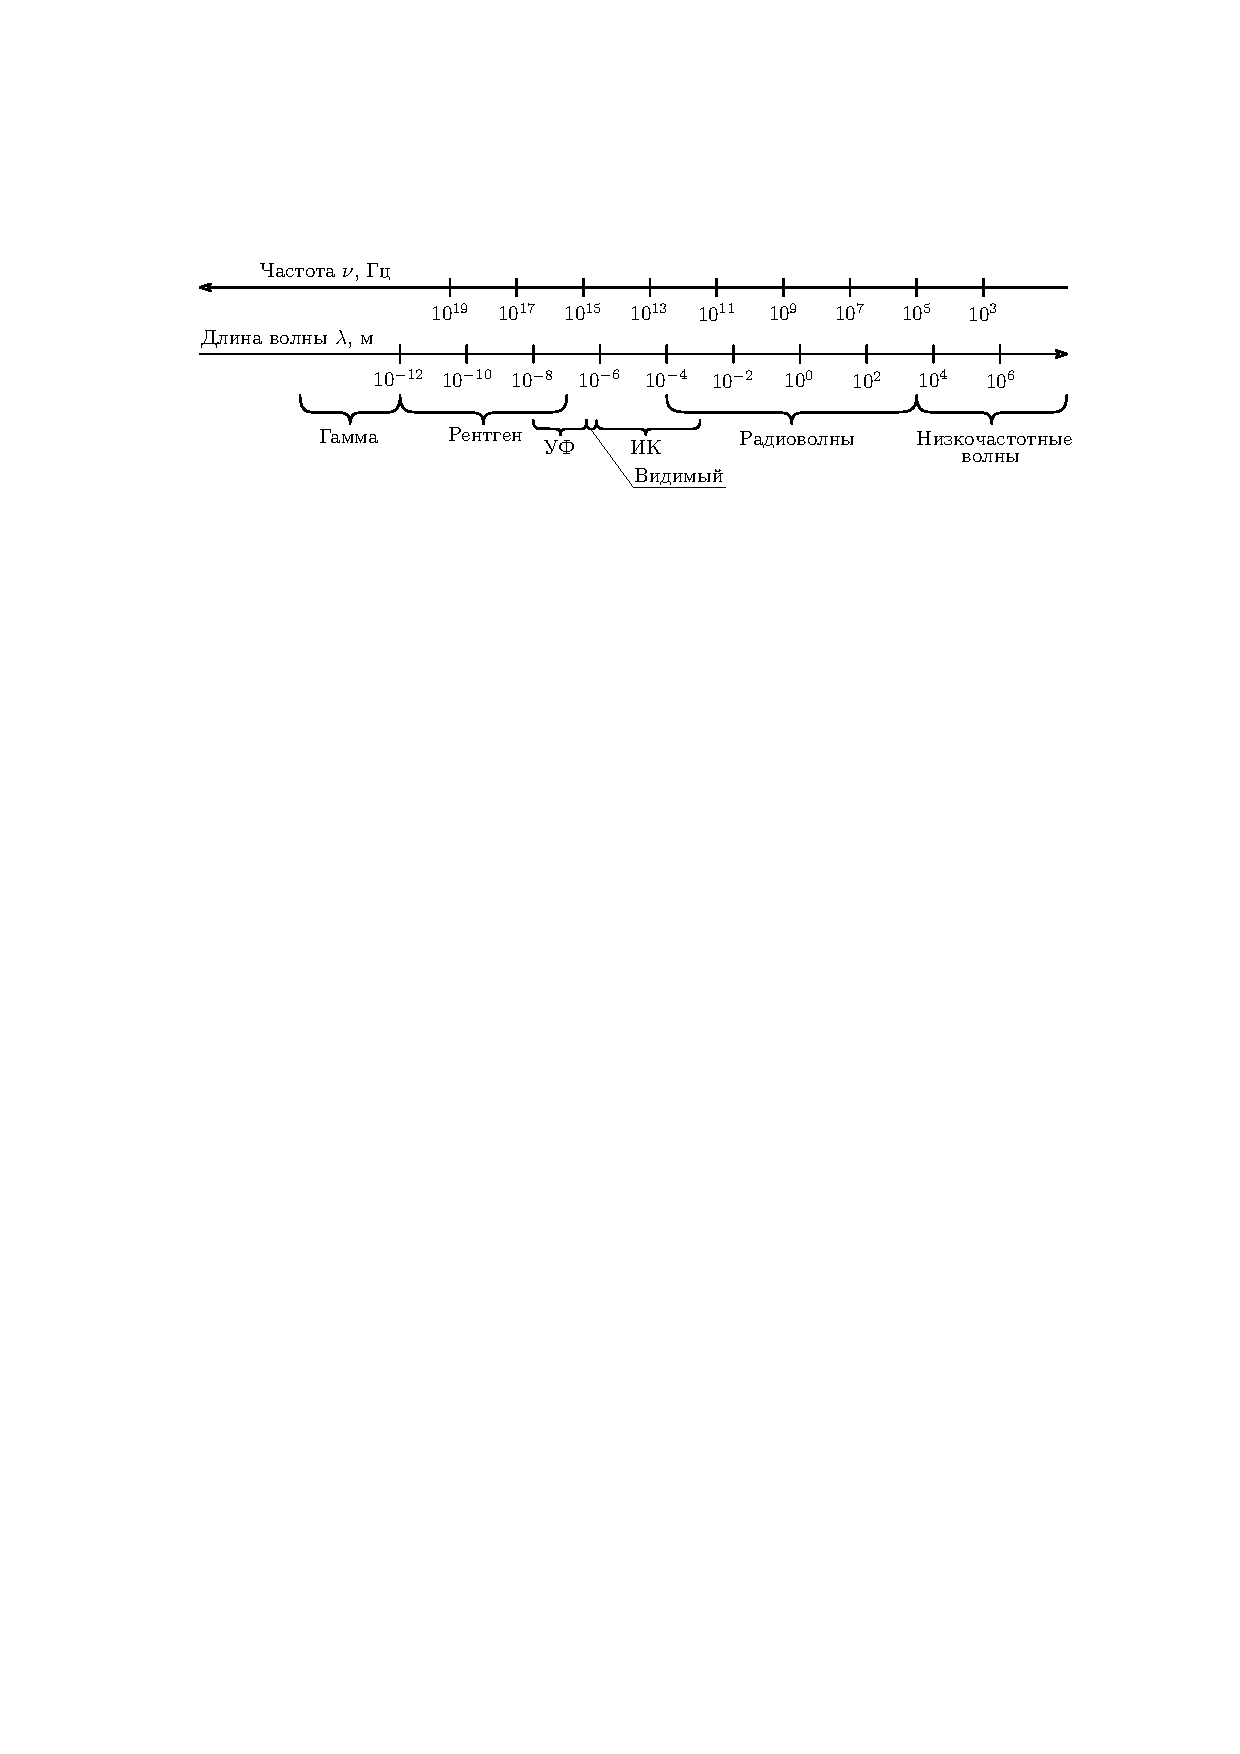
\includegraphics[width = 1\textwidth]{scale-wave.pdf}
	\caption{Шкала электромагнитных волн}
\end{figure}
\term{Ультрафиолетовые лучи}~--- излучение Солнца, ртутных ламп и т.\,п. Используются в ультрафиолетовой микроскопии, в медицине.

\term{Видимое излучение}~--- часть электромагнитного излучения, воспринимаемая глазом (от фиолетового до от красного).

\term{Инфракрасное излучение}~--- тепловое, излучается любым нагретым телом.

\term{Радиоволны} используются повсеместно в обычной жизни, это и сотовая связь, и радиолокация, и спутниковая связь, и Wi-Fi и многое другое.

\term{Низкочастотные волны}~--- диапазон, традиционно используемый в электротехнике. В промышленной электроэнергетике используется частота 50~Гц, на~которой осуществляется передача электрической энергии по линиям и преобразование напряжений трансформаторными устройствами.

%\subsection{Специальная теория относительности. Аберрация}

Обычно в СТО рассматриваются две инерциальные системы $S$ и $S'$. Время и координаты некоторого события, измеренные относительно системы $S$, обозначаются как $(t, x, y, z)$, а координаты и время этого же события, измеренные относительно системы $S'$, как $(t', x', y', z')$. Удобно считать, что координатные оси систем параллельны друг другу, и система $S'$ движется вдоль оси $x$ системы $S$ со скоростью $v$. Одной из задач СТО является поиск соотношений, связывающих $(t', x', y', z')$ и $(t, x, y, z)$, которые называются \textit{преобразованиями Лоренца}. Общий вид \term{преобразований Лоренца} в векторном виде, когда относительная скорость систем отсчёта имеет произвольное направление:
\begin{equation}
    t'=\gamma\cdot \left(t-\frac{(\vec{r},\vec{v})}{c^2}\right),
\end{equation}
\begin{equation}
    \vec{r'} = \vec{r} - \gamma \vec{v} t + (\gamma - 1) \cdot \frac{(\vec{r},\vec{v})\vec{v}}{v^2},
\end{equation}
где  $\gamma = \dfrac{1}{\sqrt{1 - \frac{v^2}{c^2}}} \equiv \dfrac{1}{\sqrt{1-\beta^2}}$~--- Лоренц фактор, являющийся коэффициентом масштабирования; $\vec{r}$ и $\vec{r'}$ --- радиус-векторы события относительно систем отсчёта $S$ и $S'$.

Если сориентировать координатные оси по направлению относительного движения инерциальных систем и выбрать это направление в качестве оси $x$, то преобразования Лоренца примут вид:
\begin{equation}
    t'=\gamma \left(t - \frac{v x}{c^2} \right),\quad\quad x'= \gamma \left( x-vt \right), \quad\quad y'=y,\quad\quad z'=z.
\end{equation}

При скоростях много меньше скорости света $(v\ll c)$ преобразования Лоренца переходят в \textit{преобразования Галилея}:
\begin{equation}
    t'=t,\quad\quad x'=x-vt,\quad\quad  y'=y,\quad\quad  z'=z.
\end{equation}

\term{Аберрация} --- явление, состоящее в том, что движущийся наблюдатель видит светило не в том направлении, в котором он видел бы его в тот же момент, если бы находился в покое. Причём светило  смещается в сторону движения наблюдателя. Это происходит из-за конечности скорости света и из-за изменения системы отсчёта для наблюдателя.
Угол аберрационного смещения можно найти по следующей формуле
\begin{equation}\sigma=\frac{v}{c}\sin\theta,
\end{equation}
где $v$ --- скорость наблюдателя, $\theta$ --- угол между направлением вектора скорости наблюдателя и направлением на объект.

\subsection{Оптическая толщина. Закон Бугера -- Ламберта -- Бера}
\begin{wrapfigure}[10]{c}{0.4\tw}
	\centering
	\begin{tikzpicture}
		\footnotesize
		
		\foreach \x in {-1, -.9, ..., 1.01} {
		\foreach \y in {-1.5, -1.4, ..., 1.51} {
		\pgfmathsetmacro\radius{(rand+1)/60};
		\fill [lightgray] (\x + rand*.03, \y + rand*.03)  circle(\radius);
		};
		};
		
		\draw [line width=1pt](-2, 0) -- (-1, 0);
		\draw [line width=1pt, -latex](-2, 0) -- (-1.4, 0);
		\fill[left color=black, right color=lightgray] (-1, -.5pt) rectangle (1, .5pt);
		\draw [line width=1pt, lightgray](1, 0) -- (2, 0);
		\draw [line width=1pt, lightgray, -latex](1, 0) -- (1.6, 0);
		
		\draw (-1.5, .1) node[anchor=south] {$I_0$};
		\draw (1.5, .1) node[anchor=south] {$I$};
		
		\draw [latex-latex] (-1.05, -1.7) -- (1.05, -1.7);
		\draw (0, -1.7) node[anchor=north] {$L$};
	\end{tikzpicture}
	\caption{}
	\label{}
\end{wrapfigure}
Рассмотрим процесс прохождение электромагнитного излучения с интенсивностью $I_0$ через слой толщины $L$ непрозрачных частиц со средней концентрацией $n$ и сечением поглощения $\sigma$. Ясно, что интенсивность выходящего из слоя пыли излучения будет меньше начальной. Выясним, по какому закону падает интенсивность излучения в таком случае.

Для этого рассмотрим тонкий слой толщины $dx$ из всего слоя частиц. Пусть на входе в этот тонкий слой излучение имеет интенсивность $I$, а на выходе из слоя~--- $I - dI$. Часть излучения прошла сквозь тонкий слой, а часть поглотилась пылинками, общая площадь которых равна произведению их количества в этом слое на среднюю площадь поглощения. Здесь можно считать, что перекрытия частиц друг другом не происходит, так как рассматриваемый слой достаточно тонкий. Количество частиц  $dN$ в тонком слое зависит только от их концентрации и площади всего слоя, таким образом:
\begin{equation*}
	N = n S \, dx.
\end{equation*}
Тогда можно составить уравнение на изменение интенсивности излучения тонким слоем:
\begin{equation*}
	-\frac{dI}{I} = \frac{N\sigma}{S} = n\sigma \, dx.
\end{equation*}
Проинтегрируем левую и правую часть полученного уравнения:
\begin{gather*}
	-\int\limits_{I_0}^{I} \frac{dI}{I} = \int\limits_{0}^{L} n \sigma \, dx,\\
	-\ln I + \ln I_0 = n\sigma L,\\[.5pc]
	%	e^{-\ln I_0} \cdot e^{\ln I} = e^{n \sigma L},
	I = I_0 e^{-n\sigma L}. \tag{\theequation}
\end{gather*}

\term{Оптическая толщина}~--- безразмерная величина, характеризующая степень непрозрачности среды для проходящего сквозь неё излучения. В общем случае, конечно, концентрация частиц и их площадь сечения взаимодействия могут меняться от координаты, поэтому оптическая толщина определяется как
\begin{equation}
	\tau = \int n(x) \sigma(x)\,dx.
\end{equation}
Для случая постоянных $n$ и $\sigma$, как было получено выше, $\tau = n \sigma L$.

Связь интенсивности $I_0$ на входе с интенсивностью $I$ на выходе называется \term{Законом Бугера -- Ламберта -- Бера} и записывается в виде
\begin{equation}
	I = I_0 e^{-\tau}.
\end{equation}

Определим теперь среднюю длину пути $\langle l \rangle$ луча в слое до момента поглощения частицей. Будем в этом случае считать, что $L = \infty$. Вероятность поглощения луча слоем толщины $dx$ в приближении постоянной концентрации и площади эффективного сечения равна
\begin{equation*}
	p(x) = \frac{-dI(x) / dx}{I_0} = n \sigma e^{-n\sigma x}
\end{equation*}

Тогда средняя длина пути определяется как
\begin{multline*}
	\langle l \rangle 
	= \int\limits_0^\infty x p(x) \, dx 
	= \int\limits_0^\infty x n \sigma e^{-n\sigma x} \, dx =\\
	= - x e^{-n \sigma x}\big|_{0}^{\infty} -  \int\limits_0^\infty e^{-n\sigma x} \, dx 
	= 0 + \frac{1}{n \sigma} \cdot e^{-n \sigma x} \big|_0^\infty = \frac{1}{n \sigma}.
\end{multline*}
Величина $\langle l \rangle$ называется \imp{средней длиной свободного пробега} или просто \term{длиной свободного пробега}.


\subsection{Фотометрия. Показатель цвета}
\term{Фотометрическая система UBV}~--- система, разработанная для классификации звезд в зависимости от их цвета. В этой системе измеряются звездные величины звезд на трех участках спектра: $U$ (максимум чувствительности $\lambda_\text{макс}^U = 350$~нм), $B$ ($\lambda_\text{макс}^B = 430$~нм) и $V$ ($\lambda_\text{макс}^V = 550$~нм). Для звёзд спектрального класса A0V все три значения равны, поэтому такие звёзды являются фотометрическим стандартом. Одним из таких стандартов является яркая звезда северного неба Вега.

\term{Показатель цвета} $(B-V)$~--- разница блеска объекта в фильтрах $B$ и $V$, измеряется в звёздных величинах. Существует эмпирическая зависимость, связывающая показатель цвета $(B-V)$ и температуру  объекта,
\begin{equation}
	T = 4600 \cdot\left(\frac{1}{0.92\left(B-V\right) + 1.7} + \frac{1}{0.92\left(B-V\right) + 0.62}\right).
\end{equation}

\term{Избыток цвета} $E\left(B - V\right)$~--- разность между наблюдаемым показателем цвета звезды и нормальным, свойственным ее спектральному классу.
\begin{equation}
	E\left(B - V\right) = \left(B - V\right) - \left(B - V\right)_0 = \left(B - B_0\right) - \left(V - V_0\right) = A_B - A_V,
\end{equation}
величины $A_B$ и $A_V$~--- поглощения на голубом и видимом участках спектра.

\term{Межзвёздное поглощение}~--- суммарный эффект рассеяния и истинного поглощения света пылевыми частицами в межзвёздной среде. Известно соотношение, связывающее межзвёздное поглощение с избытком цвета,
\begin{equation}
	\frac{A_V}{E\left(B - V\right)} = R \approx 3.1.
\end{equation}

%Поглощение света в среде зависит от длины волны, и установлена эмпирическая зависимость
%\begin{equation}
%A_B - A_V = 1.086 \bigl(\tau\left(B\right) - \tau\left(V\right)\bigr),
%\end{equation}
%где $\tau\left(B\right)$ и $\tau\left(V\right)$~---  оптические толщины в голубом и видимом диапазоне.

\subsection{МКТ и термодинамика}
\term{Молекулярно-кинетическая теория} изучает процессы, происходящие в макроскопических телах, на основе предположения о том, что вещество состоит из частиц, движение которых подчиняется законам механики Ньютона.

\term{Уравнение Менделеева-Клайперона} является следствием этой теории и~связывает давление $(P)$, объем $(V)$ и температуру $(T)$ идеального газа:
\begin{equation}
    PV = \nu R T,
    \label{eq:mkt-idial-gas}
\end{equation}
здесь $R = 8.31~\text{м}^2 \cdot \text{кг} \cdot \text{с}^{-2} \cdot \text{К}^{-1} \cdot \text{моль}^{-1}$~--- \imp{универсальная газовая постоянная}, а $\nu$~--- количество вещества идеального газа. Иначе, можно записать
\begin{equation}
    P = nkT =  \frac{\rho}{\mu}RT,
    \label{eq:mkt-p}
\end{equation}
где $n$~--- концентрация, $k$~--- постоянная Больцмана, $\rho$~--- плотность газа, $\mu$~--- молярная масса.

Частицы газа имеют равномерное распределение в предоставленном пространстве и распределение Максвелла по энергиям, то есть вероятность, что частица обладает энергией $E$ равна
\begin{equation}
    f_E(E) = \frac {2\pi \sqrt{E}}{\sqrt{(\pi kT)^3}}  \exp\left(\frac {-E} {kT} \right).
    \label{eq:maxwell}
\end{equation}
После некоторых математических преобразований несложно получить выражение для средней энергии $\langle E \rangle$ частиц идеального газа:
\begin{equation}
    \langle E \rangle = \frac{3}{2}kT,
\end{equation}
следовательно, \term{среднеквадратичная скорость} определяется, как
\begin{equation}
    \langle v^2 \rangle = \frac{3kT}{m}.
\end{equation}
Однако, исходя из распределения \eqref{eq:maxwell}, \imp{наиболее вероятная скорость} частиц
\begin{equation}
    v_\text{н.в.} = \sqrt{\frac{2kT}{m}}.
\end{equation}

\term{Первое начало термодинамики} гласит:
\begin{equation}
    \delta Q = dU + \delta A,
\end{equation}
где $\delta Q$~--- подведенная теплота, $d U$~--- изменение внутренней энергии газа, $\delta A$~--- работа газа.

\imp{Внутренняя энергия} газа определяется соотношением
\begin{equation}
    U = \frac{i}{2}RT,
\end{equation}
здесь $i$~--- количество степеней свободы частиц газа.

\term{Теплоёмкость идеального газа}~--- отношение количества сообщённой газу теплоты $\Delta Q$, к произошедшему изменению температуры $\Delta T$, в расчёте на один моль:
\begin{equation}
    C = \frac{\delta Q}{dT}
\end{equation}

\term[изотермический процесс]{Изотермический} процесс~--- при котором температура газа не изменяется:
\begin{equation}
    PV = \const, \quad\quad C_T = +\infty,
\end{equation}
индекс теплоёмкости соответствует величине, постоянной в течение процесса.

\term[изохорический процесс]{Изохорический} процесс~--- когда объём, занимаемый газом, не изменяется:
\begin{equation}
    \frac{P}{T} = \const, \quad\quad C_V = \frac{i}{2}R.
\end{equation}

\term[изобарический процесс]{Изобарический} процесс~--- тот, при котором давление газа не изменяется:
\begin{equation}
    \frac{V}{T} = \const, \quad\quad C_P = \frac{i+2}{2}R = C_V + R.
\end{equation}

\term[адиабатический процесс]{Адиабатический} процесс~--- процесс, в котором количество подведенной теплоты $\delta Q$ равно нулю:
\begin{equation}
    P V^\alpha = \const, \quad\quad C_Q = 0,
\end{equation}
где $\alpha = C_P/C_V$~--- показатель адиабаты.

\subsection{Атмосфера Земли}
Применим знания о МКТ для поиска характерной высоты атмосферы Земли в двух её моделях: изотермической и адиабатической атмосферах. Прежде, чем приступим к поиску, несколько фактов об атмосфере Земли. Давление у поверхности Земли в среднем составляет 
\begin{equation*}
	p_0 = 1~\text{атм} = 101325~\text{Па} = 760~\text{мм рт. ст}.
\end{equation*}
Наблюдаемые отклонения от среднего значения незначительны для последующих выкладок, так как составляют не более $5\%$. 

Средняя температура воздуха у поверхности $T_0 \approx 12^\circ\text{C} = 285~\text{K}$. Молярная масса воздуха, средневзвешенное молярных масс его компонент, $\mu_0 = 29~\text{г}/\text{моль}$. 

\paragraph{Изотермическая атмосфера} Падение давления воздуха с увеличением высоты можно описать математически~\cite{barometric-formula-isotermal}. Для этого рассмотрим тонкий слой воздуха толщиной $dh$, выделим в нём фрагмент с площадью $dS$. Пусть масса воздуха в этом фрагменте равна $dm$.  Представим, что воздух в выделенном фрагменте окружен невесомой тонкой оболочкой~--- не перемешивается с окружающим воздухом и находится в равновесии. Которое достигается благодаря равенству нулю равдействующей трёх сил: силы давления воздуха снизу $F_\uparrow = p\d S$, силы давления воздуха сверху $F_\downarrow = -(p + dp)\d S$ и силы тяжести $F_g = -g\d m$, действующей на выделенный слой. Здесь $dp < 0$, так как с высотой давления, очевидно, уменьшается, потому что все меньший столб воздуха оказывает давление на рассматриваемый слой. Итак,
\begin{gather}
	F_\uparrow + F_\downarrow + F_g = 0,\nonumber\\
	p \d S - (p + dp) \d S - g \d m = 0,\nonumber\\
	- dp\d S = g \rho \d V = g \rho \d h \d S,\nonumber\\
	dp = - g \rho \d h. \label{eq:isotherm-atm-dp}
\end{gather}

Из уравнения состояния идеального газа \eqref{eq:mkt-p}, считая воздух таковым, выразим плотность воздуха $\rho$:
\begin{equation*}
	\rho = \frac{p \mu}{RT}.
\end{equation*}
Подставив полученное выражение в~\eqref{eq:isotherm-atm-dp}, получим,
\begin{equation}
	dp = - \frac{\mu g}{RT} p \d h.
	\label{eq:earth-atm-dp}
\end{equation}

Разделим переменные и проинтегрируем левую и правую часть от нуля до высоты $h$:
\begin{gather}
	\int\limits_{p_0}^{p(h)} \frac{dp}{p} = -\int\limits_0^h \frac{\mu g}{RT} dh,\nonumber\\
	\ln p(h) - \ln p_0 = -\frac{\mu g h}{RT},\nonumber\\
	p(h) = p_0 \exp \left[ -\frac{\mu g h}{RT} \right]. \label{eq:earth-atm-isot}
\end{gather}
Полученное равенство называется \imp{барометрической формулой для изотермической атмосферы}. Из нее следует, что характерная (давление уменьшилось в $e$ раз) высота изотермической атмосферы
\begin{equation*}
	H_{T=\const} = \frac{RT}{\mu g} \simeq 8~\text{км}.
\end{equation*}

\paragraph{Адиабатическая атмосфера}
Конечно, предположение об изотермичности атмосферы достаточно грубо. Рассмотрим модель, в рамках которой выполняется равенство $dQ = 0$ для выделенного тонкого слоя воздуха~--- адиабатическую модель атмосферы~\cite{barometric-formula-adiabatic}.

Такая модель хорошо описывает наблюдаемые в атмосфере процессы. Наибольший нагрев воздуха происходит у поверхности Земли, и чем выше, тем воздух холоднее. Это хорошо заметно в горах, где воздух холоднее, чем в нижележащих долинах. В ходе конвекции слои теплого воздуха поднимаются и расширяются, так как давление окружающего воздуха с высотой уменьшается. Работа газа по его расширению уменьшает его внутреннюю энергии~--- газ остывает.

Приступим к выводу барометрической формулы для адиабатической атмосферы. Начнем с выражений для работы газа и изменения его потенциальной энергии:
\begin{gather*}
	\delta A = p \d V,\\
	dU = C_V \nu \d T.
\end{gather*}
Запишем первое начало термодинамики для тонкого слоя воздуха:
\begin{gather}
	dQ = 0 = dU + \delta A = p \d V + C_V \nu \d T,\notag\\
	dT = - \frac{p}{C_V \nu} dV.
	\label{eq:earth-atm-dt}
\end{gather}
Выразим объем из уравнения состояния идеального газа \eqref{eq:mkt-idial-gas} и перейдем к дифференциалам:
\begin{equation}
	dV = d \left(\frac{\nu R T}{p} \right) = \frac{\nu R}{p} \d T - \frac{\nu R T}{p^2} \d p.
	\label{eq:earth-atm-dv}
\end{equation}
Подставив \eqref{eq:earth-atm-dv} в уравнение \eqref{eq:earth-atm-dt}, получим
\begin{gather*}
	dT = - \frac{p}{C_V \nu} \left( \frac{\nu R}{p} \d T - \frac{\nu R T}{p^2} \d p \right),\\
%	\left( 1 + \frac{R}{C_V} \right)\frac{dT}{T} = \frac{R}{C_V} \frac{dp}{p},\\
	\therefore \frac{dT}{T} = \frac{R}{C_V + R} \frac{dp}{p} = \frac{R}{C_p} \frac{dp}{p}.
\end{gather*}
Воспользуемся выражением~\eqref{eq:earth-atm-dp} для $dp$:
\begin{gather}
	\frac{d T}{T} = -\frac{\mu g}{C_P T} \d h,\\
	\frac{dT}{dh} =  -\frac{\mu g}{C_P} \equiv \Gamma.\label{eq:ad-therm-grad}
\end{gather}

Выражение~\eqref{eq:ad-therm-grad} показывает, что в случае адиабатической атмосферы градиент температуры $\Gamma$ является постоянной величиной. Поэтому справедливо, температура воздуха $T(h) = T_0 + \Gamma h$, где $T_0$~--- температура у поверхности. Молярная теплоёмкость воздуха при постоянном давлении $C_p = 29.15$~Дж/моль, поэтому градиент температуры~$\Gamma$ составляет~$-0.83$~К на 100~м. 

Вернемся к уравнению \eqref{eq:earth-atm-dp} и подставим в него полученное выражение для температуры, чтобы получить барометрическую формулу:
\begin{gather*}
	dp = - \frac{p \mu g}{RT(h)} dh,\\
	\int\limits_{p_0}^{p(H)} \frac{dp}{p} = - \frac{\mu g}{R} \int\limits_0^H \frac{dh}{T_0 + \Gamma h}= - \frac{\mu g}{R\Gamma} \int\limits_0^H \frac{d(T_0 + \Gamma h)}{T_0 + \Gamma h},\\
	\ln \frac{p(H)}{p_0} = - \frac{\mu g}{R\Gamma} \ln \frac{T_0 + \Gamma H}{T_0},\\
	p(H) = p_0 \left(1 + \frac{\Gamma H}{T_0} \right)^{ - \mu g /R\Gamma} =  p_0 \left(1 + \frac{\Gamma H}{T_0} \right)^{ - C_p/R}.
\end{gather*}

Отсюда получаем, что высота характерная высота адиабатической атмосферы
\begin{equation*}
	H_{dQ=0} = \left(\exp \left[ \frac{R}{C_p} \right] - 1 \right) \cdot  \frac{T_0}{\Gamma} = 9.6~\text{км}.
\end{equation*}

\begin{figure}[h]
	\centering
	\begin{tikzpicture}
	\begin{axis}[
		height	=	6cm,
		width	=	8cm,
		xlabel	=	{$H$, км},
		ylabel	=	{$p(H)$, км},
%		ylabel shift	= -1 cm,
		ymax=1,
		ymin=0,
		xmin=0,
		xmax=10,
		legend cell align=left,
			legend style={
			draw=none,
			fill=none,
			font=\scriptsize,
			at={(axis cs:1, 0.1)}, anchor=south west,
			row sep=.5pc,
			},
		]
		
		\addplot[smooth, domain=0:10, samples=200] {1 * exp(-0.029*9.81*x*1000/8.31/285) };
		\addplot[smooth, domain=0:10, samples=200, gray] {1 * (1 + 10*x/285)^(-0.029*9.81/8.31/0.00975)};
		\legend{
			$T=\const$,
			$dQ = 0$
		};
	\end{axis}
\end{tikzpicture}
\end{figure}



















\subsection{Оптические атмосферные эффекты}

В этом разделе будут рассмотрены известные оптические эффекты, возникающие в атмосфере Земли. Их можно разделить на три группы по природе происхождения. Так, \term{радуга} (см.~\ref{sec:rainbow}) формируется в ходе рефракции и отражения света в достаточно крупных каплях воды, распыленных в воздухе. Различные виды \term{гало}~--- \imp{гало} (см.~\ref{sec:halo}), \imp{зенитная дуга} (см.~\ref{sec:circumzenithal-arc}), \imp{округло-горизонтальная дуга} (см.~\ref{sec:circumhorizon-arc}) и \imp{паргелий} (см.~\ref{sec:parhelion}), формируются в результате прохождения света через кристаллы льда, находящиеся в воздухе. А такие эффекты как \imp{глория} (см.~\ref{sec:glory}), \imp{венец (корона)} (см.~\ref{sec:corona}) и \imp{радужные облака} (см.~\ref{sec:iridenscent-clouds}) формируются в силу  диффракции света на мелких каплях или кристаллах льда, или других частицах, например, частицы дыма или мелкий песок.

\subsubsection{Радуга}
\label{sec:rainbow}

\input{sections/astrophysics/optical-atmosphere-effects/tikz/rainbow-formation-tikz}
\input{sections/astrophysics/optical-atmosphere-effects/tikz/rainbow-dispersion-tikz}

Радуга~--- событие проявления преломления (рефракции) и отражения солнечного света, в каплях воды, распыленных в воздуха. Наблюдается в виде ярких разноцветных колец, перпендикулярных прямой \textsl{Солце -- наблюдатель}, с центром на ней. 

Стоит обратить внимание на возможность обобщения данной формулировки. Излучение может быть монохромным, тогда радуга будет также монохромна. Для появления радуги необязательно наличие воздуха. Данного эффекта можно достичь, распыляя воду в космосе~--- без атмосферы и гравитации. Также радуга может наблюдаться во взвеси стеклянных шариков или капель любой другой прозрачной для рассматриваемого излучения жидкости.

Рассмотрим детальнее, как формируются радужные кольца. Для упрощения расчетов солнечный свет можно считать параллельным фронтом с выделенным направлением, а капли воды с достаточной точностью сферическими. 

\begin{wrapfigure}[13]{r}{0.47\tw}
    \vspace{-1.5pc}
    \input{sections/astrophysics/optical-atmosphere-effects/tikz/rainbow-schema-tikz}
    \caption{Схема следования луча в капле при $k=2$}
\end{wrapfigure}
Представим такую каплю и отметим выделенное направление падения света пунктиром (\lookPicRef{pic:rainbow}). Рассмотрим луч, падающий на каплю на расстоянии $\rho \in [0,1]$ радиусов капли от её оси. В таком случае угол падения луча на поверхность капли $\alpha = \arcsin \rho$. Пусть $n$~--- коэффициент преломления воды, тогда по закону Снеллиуса угол преломления
\begin{equation*}
    \beta = \arcsin \frac{\sin{\alpha}}{n} = \arcsin \frac{\rho}{n}.
\end{equation*}
Так как $\beta$~--- угол между радиусом и преломленным лучем, то преломленный луч вновь пересечется с поверхностью капли на угловом расстоянии $180^\circ - 2\beta$ в сторону движения луча. 

В точке пересечения преломленного луча с поверхностью капли часть света преломится и выйдет наружу, а остальная часть отразится от внутренней поверхности под углом $\beta$ согласно закону отражения. И~на угловом расстоянии $180^\circ - 2\beta$ вновь частично преломится и покинет каплю, а частично отразится и продолжит свой путь внутри капли.

Определим \imp{порядок} радуги $k$ как число отражений луча от внутренней поверхности капли. Тогда при формировании радуги $k$-ого порядка луч света, проходящий на расстоянии $\rho$ радиусов капли от её оси с точностью до целого числа полных оборотов поворачивается на угол 
\begin{multline*}
    \omega 
        = 2(\alpha - \beta) + k (\pi - 2\beta) 
        = 2\alpha - 2\beta(k + 1) + \pi (k \!\!\!\! \mod 2) = \\
        = 2\arcsin \rho - 2(k + 1) \arcsin \frac{\rho}{n} + \pi (k \!\!\!\!  \mod 2). 
\end{multline*}

Радуга выделяется на фоне за счет своей яркости, которая достигается из-за увеличения плотности потока излучения, выходящего из капли после $k$ отражения, в конкретном направлении. Что соответствует равенству нулю производной $\partial\omega/\partial\rho$. Определим значение~$\rho$, при котором это происходит, чтобы найти угловой радиус радуги $k$-ого порядка.
\begin{gather*}
    \frac{\partial \omega}{\partial \rho} = \frac{2}{\sqrt{1 - \rho^2}} - \frac{k + 1}{\sqrt{n^2 - \rho^2}} = 0,\quad \rho \in [0,1];\\
%    \sqrt{n^2 - \rho^2} - (k + 1) \sqrt{1 - \rho^2} = 0,\quad \rho \in [0,1);\\
%    n^2 - \rho^2 = (k+1)^2(1 - \rho^2), \quad \rho \in [0,1) ;\\
    \rho = \sqrt{\frac{(k+1)^2 - n^2}{(k+1)^2 - 1}},\quad \rho \in [0, 1).
\end{gather*}

Коэффициент преломления воды в оптическом диапазоне зависит от длины волны практически линейно, принимая значения от $n_\text{к} = 1.331$ для красного света ($\lambda = 700$~нм) до $n_\text{ф} = 1.344$ для фиолетового ($\lambda = 400$~нм). Таким образом внешний край \imp{первичной} радуги имеет радиус~$42.4^\circ$ и красный цвет, а внутренний~---~$40.5^\circ$ и фиолетовый цвет,  \lookPicRef{pic:rainbow-disp-1}.
\imp{Вторичная} радуга имеет размер от~$50.4^\circ$ для красного до~$53.7^\circ$ для фиолетового, \lookPicRef{pic:rainbow-disp-2}. Важно отметить, из-за дополнительного отражения цвета вторичной радуги идут в обратном порядке относительно первичной. 

\begin{figure}[t]
    \begin{subcaptionblock}{0.3\tw}
        \centering
        \tikzsetnextfilename{rainbow-1-scheme}
        \begin{tikzpicture}[scale=1.3]
            \begin{scope}[yscale=-1]
                \drawRainbow[-1]{1}
            \end{scope}
        \end{tikzpicture}
        \caption{$k=1$}
        \label{pic:rainbow-1}
    \end{subcaptionblock}
    \hfill
    \begin{subcaptionblock}{0.3\tw}
        \centering
        \tikzsetnextfilename{rainbow-2-scheme}
        \begin{tikzpicture}[scale=1.3]
            \drawRainbow{2}
        \end{tikzpicture}
        \caption{$k=2$}
        \label{pic:rainbow-2}
    \end{subcaptionblock}
    \hfill
    \begin{subcaptionblock}{0.3\tw}   
        \centering
        \tikzsetnextfilename{rainbow-3-scheme}
        \begin{tikzpicture}[scale=1.3]
            \drawRainbow{3}
        \end{tikzpicture}
        \caption{$k=3$}
        \label{pic:rainbow-3}
    \end{subcaptionblock}
    \caption{Схема хода лучей при формировании радуги $k$-ого порядка}
    \label{pic:rainbow}
\end{figure}
\begin{figure}[h!]
    \begin{subcaptionblock}{0.3\tw}
        \centering
        \tikzsetnextfilename{rainbow-1-dispersion}
        \begin{tikzpicture}[scale=1.3]
            \begin{scope}[yscale=-1]
                \drawRainbowDispersion[-1]{1}
            \end{scope}
            \tkzDefPoint(1.2,-1.15){Label}
            \tkzLabelPoint[below=-1pt](Label){\tiny$42.4^\circ$}
            \tkzLabelPoint[left=6pt](Label){\tiny$40.5^\circ$}
        \end{tikzpicture}
        \caption{$k=1$}
        \label{pic:rainbow-disp-1}
    \end{subcaptionblock}
    \hfill
    \begin{subcaptionblock}{0.3\tw}
        \centering
        \tikzsetnextfilename{rainbow-2-dispersion}
        \begin{tikzpicture}[scale=1.3]
            \begin{scope}
                \drawRainbowDispersion{2}
            \end{scope}
            \tkzDefPoint(-0.2,-0.3){Label}
            \tkzLabelPoint[below](Label){\adjustbox{right=18pt, raise=12pt}{\tiny$53.7^\circ$}}
            \tkzLabelPoint[above](Label){\adjustbox{raise=18pt}{\tiny$50.4^\circ$}}
        \end{tikzpicture}
        \caption{$k=2$}
        \label{pic:rainbow-disp-2}
    \end{subcaptionblock}
    \hfill
    \begin{subcaptionblock}{0.3\tw}
        \centering
        \tikzsetnextfilename{rainbow-3-dispersion}
        \begin{tikzpicture}[scale=1.3]
            \drawRainbowDispersion{3}
            \tkzDefPoint(1.1,-1.3){Label}
            \tkzLabelPoint[above right=-2pt](Label){\tiny${37.7^\circ}$}
            \tkzLabelPoint[below left=-1pt](Label){\adjustbox{raise=15pt}{\tiny${42.5^\circ}$}}
        \end{tikzpicture}
        \caption{$k=3$}
        \label{pic:rainbow-disp-3}
    \end{subcaptionblock}
    \caption{Схема дисперсии лучей при формировании радуги $k$-ого порядка}
\end{figure}

Обе радуги, несложно заключить, расположены напротив Солнца и их радиус отсчитывается от противосолнечной точки. Отсюда следует важное замечание, чем ниже Солнце расположено над горизонтом, тем выше радуги первого и второго порядков. Напротив, \imp{третичная} радуга расположена со стороны Солнца на расстоянии от~$37.7^\circ$ для фиолетового до~$42.5^\circ$ для красного цветов, \lookPicRef{pic:rainbow-disp-3}.

В заключение необходимо объяснить применимость геометрической оптики в изложенных выше рассуждениях. Чаще всего радуга наблюдается до или после дождя, капли которого существенно больше капель тумана или облаков и достигают нескольких миллиметров в диаметре. Это больше характерной длины волны видимого глазом излучения на три--четыре порядка, что позволяет не учитывать волновые свойства света. В силу последних капли существенно меньшего размера могут вообще не сформировать радугу. 

\subsubsection{Гало}
\label{sec:halo}

Как было сказано выше, различные виды \imp{гало} наблюдаются в результате рефракции солнечного света в кристаллах льда, составляющих перистые облака. Эти облака в среднем находятся на высоте от 5 до 10~км, имеют температуру около $-40^\circ$C, почему состоят исключительно из кристаллов льда.


\begin{wrapfigure}[6]{r}{0.3\tw}
    \centering
    \vspace{-0.7pc}
    \newcommand{\drawPrizm}[2]{
        \tkzDefPoint(0,0){C}
	    
	    \def\R{#1}
	    \def\h{#2}
	    \def\f{0}
	    
	    \tkzDefShiftPoint[C](\R,0){x}
	    \tkzDefPointBy[rotation=center C angle \f](x)  \tkzGetPoint{R1}
	    \tkzDefPointBy[rotation=center C angle 60](R1) \tkzGetPoint{R2}
	    \tkzDefPointBy[rotation=center C angle 60](R2) \tkzGetPoint{R3}
	    \tkzDefPointBy[rotation=center C angle 60](R3) \tkzGetPoint{R4}
	    \tkzDefPointBy[rotation=center C angle 60](R4) \tkzGetPoint{R5}
	    \tkzDefPointBy[rotation=center C angle 60](R5) \tkzGetPoint{R6}
	    
	    \tkzGetPointCoord(R1){r}
	    \tkzGetPointCoord(R2){R}
	    \tkzGetPointCoord(R3){rr}
	    \tkzGetPointCoord(R4){rR}
	    \tkzGetPointCoord(R5){Rr}
	    \tkzGetPointCoord(R6){RR}
	    
	    \draw[dashed] (\rx,\ry,0) -- (\Rx,\Ry,0) -- (\rrx,\rry,0) -- (\rRx,\rRy,0);
	    \draw (\rRx,\rRy,0) -- (\Rrx,\Rry,0) -- (\RRx,\RRy,0) -- (\rx,\ry,0);
	    
	    \draw (\rx,\ry,\h) -- (\Rx,\Ry,\h) -- (\rrx,\rry,\h) -- (\rRx,\rRy,\h) -- (\Rrx,\Rry,\h) -- (\RRx,\RRy,\h) -- cycle; 
	    
	    \draw (\rx,\ry,0) -- (\rx,\ry,\h);
	    \draw[dashed] (\Rx,\Ry,0) -- (\Rx,\Ry,\h);
	    \draw[dashed] (\rrx,\rry,0) -- (\rrx,\rry,\h);
	    \draw (\rRx,\rRy,0) -- (\rRx,\rRy,\h);
	    \draw (\Rrx,\Rry,0) -- (\Rrx,\Rry,\h);
	    \draw (\RRx,\RRy,0) -- (\RRx,\RRy,\h);
    }

    \tdplotsetmaincoords{70}{165}
    \begin{tikzpicture}[tdplot_main_coords]
        \drawPrizm{0.4}{1.5}
	\end{tikzpicture}
	\tdplotsetmaincoords{70}{185}
    \begin{tikzpicture}[tdplot_main_coords]
        \drawPrizm{0.9}{0.3}
	\end{tikzpicture}
	\caption{}
	\label{}    
\end{wrapfigure}

В условия формирования перистых облаков кристаллы льда имеют шестиугольную симметрию и являются прямоугольными шестиугольными призмами. Их боковые грани могут иметь разные пропорции, но угол между соседними всегда составляет $60^\circ$. В дальнейшем будем разделять кристаллы на два вида: пластинчатые~--- размер оснований много больше высоты призмы, и колончатые~--- наоборот, высота призмы существенно больше размеров основания.

\paragraph{$\mathbf{22^\circ}$ гало}
\begin{wrapfigure}[11]{r}{0.25\tw}
    \vspace{-1pc}
    \centering
    \begin{tikzpicture}[
        arrow/.style 2 args={
            postaction=decorate,
                decoration={
                    markings, 
                    mark=at position #2 with {\arrow{#1}}
                } 
            }
    ]
    
	    \tkzDefPoint(0,0){C}
	    
	    \def\R{2}
	    \def\f{0}
	    \def\n{1.31}
	    
	    \tkzInit[
	       xmin={-0.2*\R},
	       xmax={1.1*\R},
	       ymin={-1.1*\R},
	       ymax={1.3*\R},
	    ]
	    \tkzClip
	    
	    
	    \tkzDefShiftPoint[C](\R,0){x}
	    \tkzDefPointBy[rotation=center C angle \f](x)  \tkzGetPoint{R1}
	    \tkzDefPointBy[rotation=center C angle 60](R1) \tkzGetPoint{R2}
	    \tkzDefPointBy[rotation=center C angle 60](R2) \tkzGetPoint{R3}
	    \tkzDefPointBy[rotation=center C angle 60](R3) \tkzGetPoint{R4}
	    \tkzDefPointBy[rotation=center C angle 60](R4) \tkzGetPoint{R5}
	    \tkzDefPointBy[rotation=center C angle 60](R5) \tkzGetPoint{R6}
	    
	    \tkzDrawPolygon(R1,R2,R3,R4,R5,R6)
	    
	    \def\al{30}
	    \def\x{0.4}
	    
	    \tkzDefPointBy[homothety=center R2 ratio \x](R3) \tkzGetPoint{I}
	    \tkzDefLine[perpendicular=through I](R3,R2) \tkzGetPoint{I'}
	    
	    \def\bet{asin(sin(\al / 180 * pi) / \n)}
	    \def\b{\R * (sqrt(3) / 2  + (0.5 - \x) * tan(pi / 2 - \bet))}
	    \def\xo{(\b + sqrt(3) * \R) / (tan(pi / 2 - \bet) + sqrt(3))}
	    \def\yo{sqrt(3) * \xo - sqrt(3) * \R}
	    
	    \tkzDefPoint(\xo,\yo){O}
	    \tkzDefLine[perpendicular=through O](R1,R6) \tkzGetPoint{O'}
	    
	    \tkzInterLL(I,I')(O,O') \tkzGetPoint{T}
	    
	    \tkzDefPointBy[rotation=center I angle {-180 + \al}](T) \tkzGetPoint{x}
	    \tkzDefPointBy[homothety=center I ratio 0.4](x) \tkzGetPoint{A}
	    
	    \tkzFindAngle(I,O,T) \tkzGetAngle{gam}
	    \def\del{asin(\n * sin(\gam / 180 * pi)) * 180 / pi}
	    
	    \tkzDefPointBy[rotation=center O angle {180 - \del}](T) \tkzGetPoint{x}
	    \tkzDefPointBy[homothety=center O ratio 0.5](x) \tkzGetPoint{D}
	    
	    \tkzDrawSegments[semithick, arrow={latex}{0.3}](A,I)
	    \tkzDrawSegments[semithick, arrow={latex}{0.5}](I,O)
	    \tkzDrawSegments[semithick, arrow={latex}{0.9}](O,D)
	     
	    \tkzDrawLines[dashed, add=0.5cm and 0.5cm](I,T O,T)
	    
	    \tkzMarkRightAngles[size=0.2](R3,I,T T,O,R6)
	    
	    \tkzMarkAngle[arc=lll, size=0.5](T,I,O)
	    \tkzLabelAngle[pos=0.75](T,I,O){\footnotesize$\beta$}
	    
	    \tkzMarkAngle[arc=lll, mark=|, size=0.4, mksize=2](I',I,A)
	    \tkzLabelAngle[pos=0.6](I',I,A){\footnotesize$\alpha$}
	    
	    \tkzMarkAngle[line width = .3pt, size=0.01](I,O,T)
	    \tkzMarkAngle[arc=ll, size=0.3](I,O,T)
	    \tkzLabelAngle[pos=0.5](I,O,T){\footnotesize$\gamma$}
	    
	    \tkzMarkAngle[arc=ll, mark=|, size=0.3, mksize=2](D,O,O')
	    \tkzLabelAngle[pos=0.5](D,O,O'){\footnotesize$\delta$}
	    
	    \tkzMarkAngles[size=0.2](O,T,I R2,R1,R6 R3,R2,R1 R1,R6,R5)
	    \tkzLabelAngle[pos=0.5](O,T,I){\scriptsize$120^\circ$}
	   	    
	    \tkzDrawPoints(I, T, O, R1, R2, R6)
	\end{tikzpicture}
	\caption{}
	\label{}
\end{wrapfigure}
Яркая окружность вокруг Солнца, угловой радиус которой оставляет около $22^\circ$ в зависимости от длины волны излучения. Формируется в произвольно расположенных кристаллах в результате рефракции света на двух, следующих через одну, боковых гранях.

В зависимости от угла падения света на первую грань меняется угол итогового преломления, минимальная величина которого~--- примерно $22^\circ$. В силу экстремальности этого значения, наибольшее число кристаллом преломляют солнечный свет именно под этим углом.

Детально расмотрим геометрию формирования $22^\circ$ гало. Пусть~$\alpha$~--- угол падения луча на боковую грань $\mathcal{A}$ в проекции на нормальную к оси кристалла плоскость, а $n$~--- коэффициент преломления льда. Тогда, исходя из закона Снеллиуса, угол преломления $\beta$ определяется соотношением $\sin \alpha = n \sin \beta$. Выберем место падения луча и угол $\alpha$ такими, чтобы преломленный луч упал на несмежную и непротивоположную боковую грань $\mathcal{B}$. Обозначим угол падения на эту грань как $\gamma$. Учитывая геометрию кристаллов льда, несложно показать, что угол между нормалями к $\mathcal{A}$ и $\mathcal{B}$ составляет $120^\circ$, таким образом $\gamma = 60^\circ - \beta$. Снова применяя закон Снеллиуса, получаем, $\sin \delta = n \sin \gamma$. Окончательно, угол преломления исходного луча кристаллом льда $\rho =  \alpha + \delta - 60^\circ$.

Из полученных соотношений имеем зависимость $\rho(\alpha)$. Максимум плотности излучения наблюдается близ экстремума данной функции, то есть при $\rho'(\alpha) = 0$. Что соответствует $\alpha_0 = 40.9^\circ$ и $\rho(\alpha_0) = 21.8^\circ$ при $n=1.31$. 

\paragraph{Паргелий}

Когда пластинчатые кристаллы дрейфуют вниз под действием силы тяжести, из-за сопротивления воздуха и своей формы они ориентируются определённым образом: их основания почти горизонтальны. Такая конфигурация стабильна, то есть небольшие отклонения создают корректирующие силы, возвращающие кристаллы в близкое горизонтальному положение. Таким образом у пластинчатых кристаллов только одна степень свободы~--- вращение в горизонтальное плоскости.

Эта особенность пластинчатых кристаллов проявляется в виде увеличения яркости $22^\circ$ гало на высоте в окрестности высоты Солнца над горизонтом. Данное явление считают отдельным видом гало~--- \imp{паргелием}. А 

\paragraph{Паргелический круг}

В силу горизонтальной ориентации пластинчатых кристаллов происходит следующее. Солнечный свет, попадая в пластинчатый кристалл через верхнюю торцевую грань, один или более раз отражаясь от боковых граней, выходит из кристалла через нижнюю торцевую грань под тем же углом к горизонту, однако, имея отличное по азимуту направление. Таким образом равномерно распределенные в воздухе пластинчатые кристаллы отражают солнечный свет во всех направлениях в горизонтальной плоскости, сохраняя угол следования лучей к горизонту.

В результате описанных выше отражений при подходящих метеорологических условиях и высоте Солнца наблюдатель может увидеть полную окружность, параллельную горизонту, проходящую через Солнце.

\begin{tikzpicture}
		\begin{axis}[
			height	=	7cm,
			width	=	7cm,
			xmin = -2.1,
			xmax = 2.1,
			ymin = -2.1,
			ymax = 2.1,
			grid=none,
			axis line style={draw=none},
			every tick/.style	=	{ draw=none},
			yticklabels={,,},
			xticklabels={,,} 
			]
			
			\addplot+[smooth, dashes, gray] table[x=x, y=y] {data/tanget_arc_grid-80.txt};
			\addplot+[smooth, dashes, gray] table[x=x, y=y] {data/tanget_arc_grid-70.txt};
			\addplot+[smooth, dashes, gray] table[x=x, y=y] {data/tanget_arc_grid-60.txt};
			\addplot+[smooth, dashes, gray] table[x=x, y=y] {data/tanget_arc_grid-50.txt};
			\addplot+[smooth, dashes, gray] table[x=x, y=y] {data/tanget_arc_grid-40.txt};
			\addplot+[smooth, dashes, gray] table[x=x, y=y] {data/tanget_arc_grid-30.txt};
			\addplot+[smooth, dashes, gray] table[x=x, y=y] {data/tanget_arc_grid-20.txt};
			\addplot+[smooth, dashes, gray] table[x=x, y=y] {data/tanget_arc_grid-10.txt};
			\addplot[smooth, gray] table[x=x, y=y] {data/tanget_arc_grid0.txt};
			\addplot+[smooth, dashes, gray] table[x=x, y=y] {data/tanget_arc_grid10.txt};
			\addplot+[smooth, dashes, gray] table[x=x, y=y] {data/tanget_arc_grid20.txt};
			\addplot+[smooth, dashes, gray] table[x=x, y=y] {data/tanget_arc_grid30.txt};
			\addplot+[smooth, dashes, gray] table[x=x, y=y] {data/tanget_arc_grid40.txt};
			\addplot+[smooth, dashes, gray] table[x=x, y=y] {data/tanget_arc_grid50.txt};
			\addplot+[smooth, dashes, gray] table[x=x, y=y] {data/tanget_arc_grid60.txt};
			\addplot+[smooth, dashes, gray] table[x=x, y=y] {data/tanget_arc_grid70.txt};
			\addplot+[smooth, dashes, gray] table[x=x, y=y] {data/tanget_arc_grid80.txt};
			\addplot[smooth] table[x=x, y=y] {data/tanget_arc_grid_border.txt};
			
			\addplot+[only marks, mark = o, mark options={scale=0.2, black}] table[x=x, y=y] {data/tanget_arc_h45.txt};
			\addplot+[only marks, mark = o, mark options={scale=0.2, darkgray}] table[x=x, y=y] {data/tanget_arc_h30.txt};
			\addplot+[only marks, mark = o, mark options={scale=0.2, gray}] table[x=x, y=y] {data/tanget_arc_h15.txt};
			\addplot+[only marks, mark = o, mark options={scale=0.2, lightgray}] table[x=x, y=y] {data/tanget_arc_h0.txt};
			
		\end{axis}
	\end{tikzpicture}

\paragraph{Зенитная дуга}

Радужная дуга недалеко от зенита~--- результат рефракции солнечного света в пластинчатых кристаллах льда, расположенных над наблюдателем. 


% todo: Как пересечение 22 гало и паргелического круга



\subsubsection{Округло-горизонтальная дуга}
\label{sec:circumhorizon-arc}

\subsubsection{Радужные облака}
\label{sec:iridenscent-clouds}
\subsubsection{Венец (корона)}
\label{sec:corona}
\subsubsection{Глория}
\label{sec:glory}
\subsection{Давление и температура в центре звезды}
В данном разделе найдем оценку для давления и температуры в центре звезды. Для этого рассмотрим такую модель, пусть звезда~--- однородное газовое облако радиусом $R$. Пусть плотность звезды равна $\rho$, а вещество~--- водородоподобная плазма, такое допущение справедливо для звёзд на главной последовательности. Тогда средняя масса частиц газа составляется примерно $m = 0.5m_p$, потому вещество состоит из одинакового числа протонов и электронов, так как в целом оно нейтрально, а $m_e \ll m_p$.

Аналогично поиску высоты атмосферы рассмотрим тонкий слой вещества высоты $dr$ с площадью сечения $dS$ на расстоянии $r$ от центра звезды. Пусть его масса  равна $dm$. На слой действуют три силы: сила давления газа снизу $F_\uparrow = p(r)\,d S$, сила давления газа сверху $F_\downarrow = -p(r + \,d r)\,d S$ и сила гравитационного притяжения $F_g = -GM(r)/r^2\,d m$ от массы, находящейся внутри сферы радиуса $r$, так как суммарное воздействие от внешней оболочка равно нулю. Стационарность звезды обеспечивается балансом этих сил, значит
\begin{gather*}
	F_\uparrow + F_\downarrow + F_g = 0,\\
	p(r)\,d S - p(r + \,d r)\,d S - \frac{GM(r)}{r^2}\,d m = 0,\\
	p\,d S - (p + dp)\,d S - \frac{4\pi G \rho r^3}{3r^2} \cdot \rho \,d r \,d S = 0,\\
%	-dp = \frac{4\pi G \rho^2}{3} \cdot r\,d r,\\  
	\int\limits_{p_0}^0 -dp = \int\limits_{0}^R \frac{4\pi G \rho^2}{3} \cdot r\,d r,\\
 	p_0 = \frac{4\pi G \rho^2 R^2}{6} = \frac{GM\rho}{R}.
\end{gather*}

Приняв вещество звезды за идеальный газ, получим:
\begin{gather*}
	p_0 = \frac{G M \rho}{R} = n k T_0,\\
	T_0 = \frac{G M \rho}{n k R} = \frac{G M \rho m}{\rho k R} = \frac{G M m_p}{2k R}.
\end{gather*}
Для Солнца имеем $p_0 \sim 10^{14}$~Па, $T_0 \sim 10^7$. В действительности же давление в центре Солнца оценивается на два порядка большим значением, однако температуры рассмотренная модель дает похожий на действительность результат.
\subsection{Теорема Гаусса}
\label{sec:gauss}

Пусть элементарная площадка имеет площадь $dS$, нормаль $\vec n$, определим вектор этой площадки, как $\vec{dS} = \vec n \,d S$. Пусть напряженность гравитационного поля (ускорение свободного падения) постоянно в малой окрестности площадки, тогда поток напряженности поля через площадку равен $d\Phi = \scalar{g}{dS} = g \,d S \cos \theta$, где $\theta$~--- угол поворота от вектора $\vec g$ к вектору $\vec {dS}$.  

\paragraph{Теорема Гаусса} Пусть внутри замкнутой поверхности $s$ заключена масса $M$, тогда полный поток напряженности гравитационного поля через поверхность $s$ равен
\begin{equation}
    \Phi = \oint\limits_s \scalar{g(r)}{dS} = -4\pi G M.
\end{equation}    
\imp{Доказательство}\,\cite{кириченко2011электричество}. Начнем с самого простого случая~--- точечной массы $M$, а в качестве замкнутой поверхности $s$ возьмём сферу, центр которой совпадает с положение точечной массы, радиусом $R$. Тогда в любой точке поверхности модуль вектора напряженности гравитационного поля будет равен $g = GM/R^2$, а направление $\vec g$ будет противоположным направлению нормалей к сфере (считаем нормали внешними). Следовательно,
\begin{equation*}
    \Phi = \oint\limits_s \scalar{g(r)}{dS} = -\oint\limits_s \frac{GM}{R^2} \,d S = -\int\limits_{4\pi} \frac{GM}{R^2} R^2 \,d \Omega = -4\pi GM.\footnote{см. раздел \ref{subsec:solid-angle}}
\end{equation*}
Этот случай легко обобщается на несферические поверхности, потому что, как можно заметить, подынтегральное выражение не зависит от расстояния элементарной площадки от точечной массы.

Пусть теперь точечная масса $M$ находится вне поверхности $s$. В таком случае суммарный поток через поверхность должен быть равен нуль, потому как внутри поверхности нет никакой массы. Действительно, пустим луч из точечной массы через поверхность, ясно, луч пересечет поверхность дважды, причем первый раз нормаль к поверхности с вектором ускорения свободного падения будет образовывать острый угол ($\cos \theta > 0$), а во втором~--- тупой ($\cos \theta < 0$). Рассмотрим телесный угол $d \Omega$ вокруг этого направления и найдём вклад в суммарный поток от потоков через элементарные площадки в данном телесном углу:
\begin{equation*}
    d\Phi = d\Phi_+ + d \Phi_- = \frac{GM}{R_1^2} R_1^2 \,d \Omega -  \frac{GM}{R_2^2} R_2^2 \,d \Omega = 0.
\end{equation*}
Так как вклад не зависит от выбора направления, то теорема в этом случае доказана.

До этого момента в расчет брались только выпуклые относительно точечной массы поверхности. Поступая аналогично предыдущему случаю, можно показать, что если масса находится внутри поверхности, то луч, пересекающий поверхность не один раз, обязательно пересекает её нечетное число раз. А значит, элементарные площадки, находящиеся в телесном углу $d\Omega$ дадут вклад $d\Phi = - GM \,d \Omega$. Следовательно, общий поток будет равен $\Phi = - 4 \pi GM$.

Остается обобщить полученные результаты на случай произвольного распределения масс. В силу принципа суперпозиции полей поток напряженности суммарного поля является суммой потоков полей элементарных масс. Пусть $\rho(\vec r)$~--- распределение плотности внутри поверхности. Тогда суммарный поток
\begin{equation*}
    \Phi = \int\limits_V -4\pi G \rho(\vec r) \,d V = -4 \pi GM.
\end{equation*}

Остается сказать, что приведенные выше выкладки не зависят от природы поля и подходят для любого поля, напряженность которого подчиняется закону $C\vec{r}/r^3$. Так, для электрического поля $\Phi = 4\pi Q$, где $Q$~--- суммарный заряд внутри поверхности. На самом деле теорема Гаусса выполняется не только для полей, но и для функций, являющихся зависимостями вида $C/r^2$, так, например, суммарный поток излучения проходящий через замкнутую поверхность равен $L$, где $L$~--- суммарная светимость источников внутри поверхности.


	\section{Космология}
Будем считать, что наша Вселенная не содержит каких-либо выделенных областей
 и направлений. Её глобальные характеристики одинаковы во всех точках
 пространства в фиксированный момент времени. Это составляет суть
 \term{космологического принципа}. Он подтверждается наблюдениями: распределение
 материи во Вселенной на масштабах более~$100$\,Mpc можно считать однородным
 и изотропным, а относительные флуктуации температуры реликтового фона не
 превышают $ 10^{-5}$. Также введём следующие обозначения: величины без индексов 
 или с индексом <<e>> (от англ. \textit{emit}) обозначают наблюдаемый объект, а с 
 индексами <<$0$>> или <<o>> (от англ. \textit{observe})~--- наблюдателя.
\subsection{Кинематика}
Эволюция Вселенной соответствует \imp{космологическому принципу}, если из состояния Вселенной в один момент времени, можно получить её состояние в любой другой момент путем только лишь масштабирования. Соответственно, расстояние $D$ между двумя несвязанными объектами будет меняться по следующему закону: 
\begin{equation}
D(t) = a(t)D_0,
\label{eq}
\end{equation}
 где $a(t)$~--- масштабный фактор, $D_0$~--- а расстояние между этими объектами сейчас.

\term{Масштабный фактор}~--- это безразмерная величина, характеризующая эволюцию Вселенной. Во всех точках Вселенной в заданный момент времени масштабный фактор одинаков. В момент большого взрыва масштабный фактор принимают равным нулю, а единица соответствует текущему моменту.

Продифференциируем (\ref{eq}) по времени и разделим на себя:
\begin{equation}
\frac{1}{D} \frac{dD}{dt} = \frac{1}{aD_0} \frac{D_0 \,d a}{dt} = \frac{\dot{a}}{a} \equiv H(t).
\label{eq2}
\end{equation}
Таким образом, мы получили величину, не зависящую от расстояния, и изменяющуюся только со временем. Параметр $H(t)$ называется \term{пара\-мет\-ром Хаббла-Леметра}. А его значение сейчас, т.\,е. на данный момент~$t_0$~--- \term{постоян\-ной Хаббла}, которая равна
\begin{equation}
    H_0 = H(t_0) \approx 67...\,\frac{\text{км}}{\text{c} \cdot \text{Мпк}}.
\end{equation} 
По сути, этот параметр определяет наклон касательной к графику $a(t)$ в какой-либо момент времени, то есть показывает, расширяется Вселенная, или нет. Вторая производная \imp{масштабного фактора} по времени  определяется \term{параметром замедления} $q = -\ddot{a}a \slash \dot{a}^2$:
\begin{equation}
\frac{\ddot{a}}{a} = -qH^2.
\label{eq3}
\end{equation}
Из (\ref{eq3}) видно, что при отрицательном значении $q$ Вселенная эволюционирует с ускорением, а при положительном~--- с замедлением. Судя по наблюдениям, наша Вселенная ускоренно расширяется.

Так как выделенного направления в расширении Вселенной нет, то при отсутствии пекулярных скоростей, все объекты, подверженные расширению будут удаляться от наблюдателя радиально. Напрямую из~(\ref{eq}) следует $\dot{D} \slash D = \dot{a} \slash a = H$, то есть \term{закон Хаббла}:
\begin{equation}
v_r = HD
\label{hubble}
\end{equation}
Запишем \imp{эффект Доплера}:
\begin{equation}
\frac{\lambda_\text{o} - \lambda_\text{e}}{\lambda_\text{e}} = z \simeq \frac{v_r}{c}.
\end{equation}
Здесь $\lambda_\text{o}$~--- длина волны принимаемого света, а $\lambda_\text{e}$~--- излучаемого. Стоит заметить, что \term{красное смещение} $z$ может быть больше $1$, а последнее равенство выполняется только для $v_r \ll c.$

Рассмотрим теперь объект на небольшом расстоянии $D = cdt$ от наблюдателя таком, что $v_r \slash c = d \lambda \slash \lambda \ll 1$. Используя \imp{закон Хаббла}, получаем:
\begin{equation}
\frac{v_r}{c} = \frac{d \lambda}{\lambda} = \frac{D \dot{a}}{ca} = dt \frac{\dot{a}}{a} = \frac{da}{a}.
\end{equation}
\begin{equation}
\int_{\lambda_\text{e}}^{\lambda_\text{o}} \frac{d \lambda}{\lambda} = \int_{a}^{1} \frac{da}{a} \Rightarrow \ln \lambda_\text{o} - \ln \lambda_\text{e} = \ln 1 - \ln a \Rightarrow \frac{\lambda_\text{o}}{\lambda_\text{e}} = \frac{1}{a}
\label{dopler}
\end{equation}
%\ln \frac{\lambda_\text{o}}{\lambda_\text{e}} = \ln \frac{1}{a} \Rightarrow 
Чтобы получить связь между \imp{масштабным фактором} и \imp{красным смещением}, используем \imp{эффект Доплера}. Из него следует равенство $\lambda_{\text{o}} / \lambda_{\text{e}} = z+1.$ После подстановки в \eqref{dopler} получаем зависимость $a(z)$:
\begin{equation}
a = (1+z)^{-1}
\label{zf}
\end{equation}
Последнее уравнение очень важно в современной космологии. Оно показывает зависимомть \imp{масштабного фактора}, величины, не имеющей явного физического смысла, от \imp{красного смещения}, которое можно просто измерить. \newline \linebreak
%Определим некоторые важные размерные константы:
%\begin{enumerate}
%\item \imp{Постоянная Хаббла} $H_0 \approx 67 \text{ km} \text{ s}^{-1} \text{Mpc}^{-1} \approx 2.26 \cdot 10^{-18} \text{ s}^{-1}$
%\item \imp{Хаббловское время} сейчас $t_{H_0} = H_{0}^{-1} \approx 14.0 \text{ Gyr}$
%\item \imp{Хабблосвское расстояние} сейчас $D_{H_0} = \displaystyle \frac{c}{H_0} \approx 4.28 \text{ Gpc}$
%\end{enumerate}
Теперь продифференциируем \text{(\ref{zf}) }по времени:
\begin{equation}
\frac{da}{dt} = - \frac{1}{(1+z)^{2}} \frac{dz}{dt} = - \frac{a}{1+z} \frac{dz}{dt},
\label{dadz}
\end{equation}
разделим на $a$:
\begin{equation}
H = \frac{1}{a} \frac{da}{dt} = \frac{d\ln (a)}{dt} = - \frac{1}{1+z} \frac{dz}{dt},
\end{equation}

\subsection{Динамика}
В этом разделе будут приведены \imp{иллюстрации} выводов некоторых основных уравнений в динамике эволюции плоской, однородной и изотропной Вселенной, заполненной материей, излучением (включая релятивистские нейтрино и т. п.) и тёмной энергией.
\subsubsection{Вселенная, заполненная материей.}
Выделим небольшую сферу радиусом $R(t) = R_0 a(t) \ll D_{\text{H}_0}$, массой $M$ и средней плотностью $\rho = M / \frac{4}{3} \pi R^3 $. В силу изотропности Вселенной пространство вокруг выбранной нами области гравитационно на неё не действует. Запишем выражение для ускорения свободного падения на границе этой сферы. По закону Всемирного тяготения
\begin{equation}
g = \ddot{R} = -\frac{GM}{R^2} = -\frac{4 \pi G \rho R^3}{3 R^2} = -\frac{4 \pi}{3} G \rho R.
\label{dmov}
\end{equation}
Таким образом мы получили \term{уравнение движения} для нашей Вселенной. 
%Для удобства использования перепишем его в другой форме:
%\begin{equation}
%r_0 \ddot{a} = -\frac{4 \pi G \rho_0 r_{0}^{3}}{3r_{0}^{2} a^2} = -\frac{4 \pi G \rho_0 r_{0}}{3 a^2}.
%\end{equation}
%Разделив уравнение на $r_0$, получаем:
%\begin{equation}
%\ddot{a} = -\frac{4 \pi G \rho_0}{3} a^{-2},
%\label{mov}
%\end{equation}
%где $\rho_0$~--- плотность Вселенной на данный момент. Один раз проинтегрируем (\ref{mov}). 
%$$
%\ddot{a} = \frac{d}{dt} \dot{a} = \frac{d \dot{a}}{da} \frac{da}{dt} = \frac{d \dot{a}}{da} \dot{a}
%$$
%Подставим эту замену в (\ref{mov}):
%\begin{equation}
%\dot{a} \frac{d \dot{a}}{da} = -\frac{4 \pi G \rho_0}{3} a^{-2}
%\end{equation}
%%В итоге:
%После интегррования получаем
%%$$
%%\int \dot{a} d \dot{a} = -\frac{4 \pi G \rho_0}{3} \int a^{-2} da
%%$$
%%$$
%%\frac{1}{2} \dot{a}^2 = -\frac{4 \pi G \rho_0}{3} \frac{a^{-1}}{-1} + C
%%$$
%\begin{equation}
%\frac{1}{2} \dot{a}^2 - \frac{4 \pi G \rho_0}{3} a^{-1} = C
%\end{equation}
%Это выражение по своему виду является законом сохранения энергии. Определим теперь ыид константы $C$. 
Проинетгрируем его один раз.
\begin{equation}
\ddot{R} = \frac{d}{dt} \dot{R} = \frac{d \dot{R}}{dR} \frac{dR}{dt} = \frac{d \dot{R}}{dR} \dot{R}
\label{change}
\end{equation}
Подставим эту замену в (\ref{dmov}):
\begin{equation}
\dot{R} \frac{d \dot{R}}{dR} = -\frac{GM}{R^2}
\end{equation}
%В итоге:
После интегрирования получаем
%$$
%\int \dot{a} d \dot{a} = -\frac{4 \pi G \rho_0}{3} \int a^{-2} da
%$$
%$$
%\frac{1}{2} \dot{a}^2 = -\frac{4 \pi G \rho_0}{3} \frac{a^{-1}}{-1} + C
%$$
\begin{equation}
\frac{1}{2} \dot{R}^2 - \frac{GM}{R} = C
\label{menerg}
\end{equation}
Это выражение по своему виду является законом сохранения энергии. Определим теперь вид константы $C$. Будем считать известными значения $H_0, R_0$ и $\rho_0$ в данный момент времени $t_0$. По \imp{закону Хаббла} $(dR / dt)_{t = t_0} = R_0H_0$. Также $M = \frac{4}{3} \pi R_{0}^{3} \rho_0$. Подставим эти выражения в (\ref{menerg}):
\begin{multline}
C = \frac{1}{2} \left(\frac{dR}{dt}\right)_{t = t_0} - \frac{4 \pi G \rho_0 R_{0}^{3}}{R_0}  =\\ 
= \frac{1}{2} R_{0}^{2} H_{0}^{2} - \frac{4 \pi G}{3} \rho_0 R_{0}^{2} = \frac{1}{2} R_{0}^{2}H_{0}^{2} \left( 1 - \frac{8 \pi G \rho_0}{3 H_{0}^{2}} \right)
\end{multline}
Соотношение $3H^2 / 8 \pi G = \rho_c$ называется \term{критической плотностью} Вселенной. Перепишем выражение для константы в более простом виде:
\begin{equation}
C = \frac{R_{0}^{2} H_{0}^{2}}{2} \left(1 - \frac{\rho_0}{\rho_{c,0}} \right).
\label{const}
\end{equation}
Тогда уравнение (\ref{menerg}) принимает следующий вид:
\begin{equation}
\dot{R}^2 = \frac{8 \pi G R_{0}^{3} \rho_0}{3R} + R_{0}^{2} H_{0}^{2} \left(1 - \frac{\rho_0}{\rho_{c,0}} \right).
\label{menerg1}
\end{equation}

Наиболее популярным и простым является сценарий развития Вселенной, при котором её плотность равна критической. В этом случае $C \equiv 0$ и уравнение (\ref{menerg1}) принимает вид
\begin{equation}
\frac{dR}{dt} = \sqrt{\frac{8 \pi G R_{0}^{3} \rho_0}{3R}} = H_0 \sqrt{\frac{8 \pi G R_{0}^{3} \rho_0}{3 H_{0}^{2} R}} = H_0 \sqrt{\frac{R_{0}^{3} \rho_0}{R \rho_{c,0}}} = H_0 \sqrt{\frac{R_{0}^{3}}{R}} \, .
\end{equation}
Решая его, получаем
\begin{equation}
\left(\frac{R}{R_0}\right)^{3/2} = a^{3/2} = \frac{3}{2} H_0 t; \quad t_0 = \frac{2}{3 H_0},
\end{equation}
Где $t$~--- возраст Вселенной на \imp{масштабном факторе} $a,$ а $t_0$~--- возраст Вселенной сейчас.

\imp{Постоянная Хаббла} в этом случае эволюционирует по следующему закону:
\begin{equation}
H(t) = \frac{\dot{R}}{R} = H_0 \sqrt{\frac{R_{0}^{3}}{R}} \cdot \frac{1}{R} = H_0 \left(\frac{R_{0}}{R}\right)^{3/2} = \frac{2}{3t},
\end{equation}
а плотность вещества, равная критической:
\begin{equation}
\rho(t) = \rho_c = \frac{3 H^2}{8 \pi G} = \frac{1}{6 \pi G t^2}.
\end{equation}
%\frac{3}{8 \pi G} \frac{4}{9 t^2} =
%Запишем \imp{закон сохранения энергии} в расчёте на единицу массы для этой сферы (равенство нулю достигается в выбранной нами модели):
%\begin{equation}
%\frac{\dot{r}^2}{2} - \frac{GM}{r} = E = 0
%\end{equation}
%Так как $r = r_0 a(t)$, а $M = \frac{4}{3} \pi r^3 \rho$, (2.1) принимает следующий вид:
%\begin{equation}
%\frac{\dot{a}^2}{2} - \frac{4 \pi}{3} G a^2 \rho = 0
%\end{equation}
%Умножим обе части (2.2) на $2 \slash a^2$ и выразим плотность:
%\begin{equation}
%\rho = \rho_c = \frac{3}{8 \pi G} \left(\frac{\dot{a}}{a}\right)^2 = \frac{3 H^2}{8 \pi G}
%\end{equation}
%Полученное нами выражение

\subsubsection{Учёт давления. Тёмная энергия.}
Пусть теперь помимо холодной материи в нашей Вселенной есть излучение и релятивистские частицы плотностью энергии $\varepsilon_r$. Будем рассматривать их как фотонный газ. Выполняется следующее уравнение:
\begin{equation}
\varepsilon = \rho c^2,
\label{albert}
\end{equation}
Где $\rho$~--- плотность, выраженная в $kg/m^3$ (плотность массы), а $c$~--- скорость света. Если излучение находится в термодинамическом равновесии, то $\varepsilon_r = $. Давление фотонного газа задается формулой:
$$
P = \frac{\varepsilon_r}{3} = \frac{\rho_r c^2}{3}
$$
Добавим плотность излучения к плотности вещества в (\ref{dmov}) и получим \imp{уравнение движения} для Вселенной с излучением:
\begin{equation}
\ddot{R} = -\frac{4 \pi}{3} G R \left( \rho + \frac{3P}{c^2} \right).
\label{rmov}
\end{equation}
Оно совпадает с \imp{уравнением движения} из ОТО. Здесь стоит оговориться, что излучение в силу \eqref{rmov} вносит вклад как в плотность массы, так и в давление, а \imp{холодная} материя давления не оказывает. Добавим теперь в нашу Вселенную тёмную энергию.

\term{Космологическая постоянная} $\Lambda$, отвечающая за тёмную энергию, была введена А.\,Эйнштейном в уравнения ОТО для получения статичной Вселенной при их решении. Однако после решения уравнений А.\,Фридманом оказалось, что с \imp{космологической постоянной} возможны как статические, так и нестатические решения.

Из уравнений ОТО следует, что плотность \imp{тёмной энергии} постоянна:
\begin{equation}
\varepsilon_{\Lambda} = \frac{c^4 \Lambda}{8 \pi G},
\end{equation}
а давление
\begin{equation}
P_{\Lambda} = -\varepsilon_{\Lambda} = -\frac{c^4 \Lambda}{8 \pi G}.
\end{equation}
Теперь окончательно в \eqref{rmov} имеем:
$$
\rho = \rho_m + \rho_r + \rho_{\Lambda}; \quad P = P_r + P_{\Lambda} = \frac{\varepsilon_r}{3} - \varepsilon_{\Lambda}
$$
Преобразуем скобку в \eqref{rmov}:
$$
\rho + \frac{3P}{c^2} = \rho_m + \rho_r + \rho_{\Lambda} + \frac{\varepsilon_r}{c^2} - 3\frac{\varepsilon_{\Lambda}}{c^2} = \rho_m + 2\rho_r - 2\rho_{\Lambda}
$$
После подстановки в \imp{уравнение движения} получаем:
\begin{multline}
\ddot{R} = -\frac{4 \pi}{3} G R (\rho_m + 2\rho_r - 2\rho_{\Lambda}) = \\
= -\frac{4 \pi}{3} G R \left(\rho_m + 2\rho_r - \frac{c^2 \Lambda}{4 \pi G}\right) =
\\ = -\frac{4 \pi}{3} G R \left(\rho_m + 2\rho_r\right) + \frac{\Lambda c^2}{3} R.
\label{imov}
\end{multline}
Данный вид \imp{уравнения движения} наиболее удобен для интегрирования. Обычно под $\rho$ и $P$ подразумевают вклады только материи и излучения в плотность и давленние соответственно. Учитывая, что $R(t) = a(t) R_0$, перепишем \eqref{imov} в наиболее известном виде:
\begin{equation}
\frac{\ddot{a}}{a} = -\frac{4 \pi G}{3} \left( \rho + \frac{3P}{c^2} \right) + \frac{\Lambda c^2}{3}.
\label{mov}
\end{equation}

Для интегрирования уравнения \eqref{imov} нам необходимо знать, как плотности материи и излучения эволюционируют с изменением \imp{масштабного фактора}, или размера выделенной области.

Сначала рассмотрим эволюцию плотности материи. Так как масса $M$, заключённая внутри области радиса $R$ всегда остаётся внутри него, плотность этой области будет падать как куб радиуса:
\begin{equation}
\rho_{m} = \frac{3M}{4 \pi} R^{-3} = \frac{3M}{4 \pi R_{0}^{3}} a^{-3} = a^{-3} \rho_{m,0}
\label{mden}
\end{equation}
Плотность излучения эволюционирует по следующему закону:
\begin{equation}
\rho_r = a^{-4} \rho_{r,0}.
\label{rden}
\end{equation}
Вид (\ref{rden}) можно объяснить эффектом Доплера, который испытывают фотоны, догоняя удаляющегося наблюдателя. Пространственная концентрация фотонов в выделенной области будет падать, как и плотность материи, обратно пропорционально объёму области. Также из-за эффекта Доплера (см. \ref{dopler}), энергия каждого фотона будет уменьшаться обратно пропорционально \imp{масштабному фактору}: $\epsilon = hc/\lambda \sim a^{-1}$. Совокупность этих эффектов даёт нам \eqref{rden}.

Получить это выражение более формально можно, рассматривая излучение как идеальный газ, расширяющийся адиабатически. Запишем его работу:
\begin{equation}
dA_r = d\varepsilon_r V = -P dV = -\frac{\varepsilon_r}{3} dV.
\label{work}
\end{equation}
Раскроем $d\varepsilon_r V$ как приращение произведения двух функций:
$$
d\varepsilon_r V = \varepsilon_r dV + Vd\varepsilon_r,
$$
подставим в \eqref{work}:
%$$
%udV + Vdu = -\frac{u}{3} dV
%$$
$$
Vd\varepsilon_r = -\frac{\varepsilon_r}{3} - \varepsilon _r dV = -\frac{4}{3} \varepsilon_r dV
$$
$$
-\frac{3}{4} \frac{d\varepsilon_r}{\varepsilon_r} = \frac{dV}{V}
$$
После интегрирования получаем:
$$
\ln \left(\frac{\varepsilon_r}{\varepsilon_{r,0}}\right)^{-3/4} = \ln \frac{V}{V_0}
$$
\begin{equation}
\varepsilon_r = \varepsilon_r \left( \frac{V}{V_0} \right)^{-4/3} = \varepsilon_{r,0} \left( \frac{R}{R_0} \right)^{-4} = a^{-4} \varepsilon_{r,0}
\end{equation}
Заменяя плотность энергии на плотность массы с помощью \eqref{albert}, получаем \eqref{rden}.

Итак, подставим \eqref{mden} и \eqref{rden} в \imp{уравнение движения}:
\begin{multline}
\ddot{a} = -\frac{4 \pi}{3} G a \left(a^{-3} \rho_{m,0} + 2 a^{-4} \rho_r\right) + \frac{\Lambda c^2}{3} a = \\
= -\frac{4\pi G}{3} a^{-2} \rho_{m,0} -\frac{8\pi G}{3} a^{-3} \rho_{r,0} + \frac{\Lambda c^2}{3} a.
\end{multline}
Проинтегрируем это уравнение с помощью замены $\ddot{a} = \dot{a} \displaystyle \frac{d\dot{a}}{da}$ (см. \ref{change}):
\begin{equation}
\frac{1}{2} \dot{a}^2 = \frac{4\pi G}{3} a^{-1} \rho_{m,0} + \frac{1}{2}\frac{8\pi G}{3} a^{-2} \rho_{r,0} + \frac{1}{2} \frac{\Lambda c^2}{3} a^2 + C_1
\end{equation}
Разделим на $a^2$ и умножим на $2$:
\begin{equation}
\left(\frac{\dot{a}}{a}\right)^2 = \frac{8\pi G}{3} a^{-3} \rho_{m,0} + \frac{8\pi G}{3} a^{-4} \rho_{r,0} + \frac{\Lambda c^2}{3} + \frac{C_2}{a^2}.
\label{energy}
\end{equation}
Из ОТО известно, что константа $C_2$ равна $-k c^2$, где $k$ может принимать значения $-1, 0$ и $1$ и называется кривизной пространства (при $k = 0$ пространство евклидово). Далее везде будем считать $k \equiv 0$. Вынесем $8 \pi G / 3$ за скобки:
\begin{equation}
\left(\frac{\dot{a}}{a}\right)^2 = \frac{8\pi G \rho}{3} + \frac{\Lambda c^2}{3} - \frac{k c^2}{a^2}.
\end{equation}
Это равенство называется \term{уравнением энергии}. Приведём здесь ещё одну форму этого уравнения, тоже достаточно известную. 

Преопразуем $\Lambda c^2 / 3$ (т. н. $\Lambda$-член) в \eqref{energy}:
$$
\frac{\Lambda c^2}{3} = \frac{8 \pi G}{3} \frac{\Lambda c^2}{8 \pi G} = \frac{8 \pi G}{3} \rho_{\Lambda}.
$$
В левой части \imp{уравнения энергии} стоит не что иное как \imp{параметр Хаббла}! Разделим обе части уравнения на $H_{0}^{2}$:
\begin{equation}
\left(\frac{H}{H_0}\right)^2 = \frac{8\pi G}{3H_{0}^{2}} a^{-3} \rho_{m,0} + \frac{8\pi G}{3H_{0}^{2}} a^{-4} \rho_{r,0} + \frac{8 \pi G}{3H_{0}^{2}} \rho_{\Lambda}
\end{equation}
Вспомним, что отношение $3H_{0}^{2} / 8 \pi G$~--- критическая плотность Вселенной сейчас. Также введём обозначения удельной плотности: $\Omega_{i} = \displaystyle \frac{\rho_i}{\rho_c}.$ Перепишем \imp{уравнение энергии}.
\begin{equation}
\left(\frac{H}{H_0}\right)^2 = a^{-3} \Omega_{m,0} + a^{-4} \Omega_{r,0} + \Omega_{\Lambda,0}.
\end{equation}
Впоследствие мы часто будем исползовать отношение $H / H_0,$ поэтому введём для него специальное обозначение:
\begin{equation}
\frac{H}{H_0} = E(a) = \sqrt{a^{-3} \Omega_{m,0} + a^{-4} \Omega_{r,0} + \Omega_{\Lambda,0}\,}.
\label{energa}
\end{equation}
Иногда \imp{уравнение энергии} удобнее записывать, выражая \imp{масштабный фактор} через \imp{красное смещение}. Так как $a = (1+z)^{-1},$ 
\begin{equation}
E(z) = \sqrt{\Omega_{m,0}(1+z)^{3} + \Omega_{r,0}(1+z)^{4} + \Omega_{\Lambda,0}\,}.
\end{equation}

\subsection{Расстояния в космологии}
Представим, что невдалеке от нас стоит уличный фонарь. Мы хотим узнать, на каком расстоянии он от нас находится. Как же можно это расстояние измерить?
\begin{enumerate}
\item Проще всего измерить расстояние линейкой или каким-то жестким объектом известной длины.
\item Мы можем определить расстояние по времени, которое требуется свету, чтобы дойти от фонаря до нас.
\item Зная реальный размер самого фонаря, можно измерить расстояние до него по его угловому размеру.
\item Можно измерить плотность потока излучения от фонаря и по ней определить расстояние.
\end{enumerate}
В случае с обычным уличным фонарём все эти способы дадут одинаковый результат, равный расстоянию, измеренному линейкой. Пусть теперь наш уличный фонарь~--- это далёкая галактика, не связанная с нами гравитационно и не имеющая пекулярной скорости. Попробуем определить расстояние до неё предложенными выше способами.

\subsubsection{Сопутствующие координаты}
Представим сетку координат, которая расширяется вместе с Вселенной. В таких координатах любая точка Вселенной, не имеющая пекулярной скорости, неподвижна относительно сетки. Следовательно, разность координат объекта и наблюдателя в данной системе не зависит от времени.

\subsubsection*{Сопутствующее расстояние}
По сути, эта разность координат определяется количеством узлов сетки, расположенных между наблюдателем и объектом. Предположим теперь, что в данный момент времени $t_0$ количество узлов равно $N$, а расстояние между соседними~--- $l(t_0) = l_0.$ Следовательно, расстояние между наблюдателем и объектом равно $D = N l_0.$ Поскольку наша Вселенная масштабируема, мы можем вычислить $l$ для любого другого момента времени $t$: $l(t) = l_0 a(t)$ (вспомните уравнение \eqref{eq}). Напомним, что $a(t_0) \equiv 1.$ 

Если расстояние мажду соседними узлами $l(t)$ устремить к нулю, то $D$ будет вычисляться посредством интегрирования по $dl_0.$ Так как $dl_0 = dl(t) / a(t)$, а приращение расстояния $dl(t) = c dt,$ где $c$~--- скорость света,
\begin{equation}
D \equiv D_{\text{C}} = \int dl_0 = \int \frac{c dt}{a}.
\label{com}
\end{equation}
Величина $D_{\text{C}}$ называется сопутствующим расстоянием. Приведём его к более удобному для вычислений виду. Для этого домножим и разделим подынтегральное выражение на $d \ln(a)$.
$$
D_{\text{C}} = c \int_{t}^{t_0} \frac{dt}{d \ln(a)} \frac{d \ln(a)}{a} = c \int_{a}^{1} \frac{d \ln(a)}{a H(a)} = c \int_{a}^{1} \frac{da}{a^2 H(a)}
$$
Вспомним, что $da = - dz / (1+z)^{2}$ (см. \eqref{dadz}) и $a = (1+z)^{-1}$. При замене масштабного фактора на красное смещение интеграл принимает следующий вид:
$$
-c \int_{z}^{0} \frac{dz}{(1+z)^{2}} \frac{(1+z)^{2}}{H(z)} = c \int_{0}^{z} \frac{dz}{H(z)}
$$
Воспользуемся выводами, полученными в прошлом разделе:
\begin{equation}
D_{\text{C}} = D_{\text{H}_0} \int_{0}^{z} \frac{dz}{E(z)}
\label{Dc}
\end{equation}

Поскольку сопутствующее расстояние~--- это расстояние между наблюдателем и объектом в данный момент времени, то взяв интеграл \eqref{Dc} в пределах  от $z = 0$ до $z = \infty,$ мы получим нынешний размер Вселенной. Будем считать, что относительная плотность тёмной энергии $\Omega_{\Lambda,0} \simeq 0.69,$ а вкладом излучения из-за его малости пренебрежём.
\begin{equation}
R_{0,\text{C}} = D_{\text{H}_0} \int_{0}^{\infty} \frac{dz}{E(z)} \approx 3.24D_{\text{H}_0} \approx 13.9 \text{ Gpc}.
\end{equation}

\subsubsection{Световое расстояние}

%Чтобы линейки не были подвержены расширению Вселенной, они должны быть малой длины. Обозначим её за $l.$ Теперь мы можем вычислить расстояние между соседними узлами: $l N(t) = l (N_0 / a(t))$ %При расстояних, значительно меньших размера Вселенной, оно определяется следующим соотношением:
%\begin{equation}
%D_{\text{C}} \equiv \frac{D(t)}{a(t)} = D_0.
%\end{equation}
%мы измеряем расстояние между двумя соседними узлами с помощью жестких линеек одинаковой длины. Понятно, что их количество, требуемое для измерения расстояния, в разные моменты времени будет разным.
%и, прежде, чем перейти к следующему разделу, разберемся с ещё одним уравнением, позволяющим расчитать время, которое требуется свету, излученному в момент времени $t_\text{e}$, чтобы дойти до наблюдателя. Заметим, что всё, относящееся к моменту испускания обозначается с индексом "e"\text{} (от англ. \textit{emit}), а к момету наблюдения~--- с индексом "0",или "o"\text{} (от англ. \textit{observe}). В англоязычной литературе это время называется \text{} "\imp{lookback time}". Обозначим его как $t_\text{L}$.

Пусть мы наблюдаем некоторый объект на красном смнщнении $z$. Расстояние до него равно $D_{\text{C}}$, однако из-за расширения вселенной оно не будет равно тому расстоянию, которое пройдёт свет от объекта да наблюдателя. Световое расстояние складывается из небольших отрезков $c dt$, то есть, чтобы его найти, нужно вычислить следующий интеграл:

$$
D_\text{L} = \int_{t_\text{e}}^{t_\text{o}} c dt = c \int_{a_\text{e}}^{1} \left(\frac{dt}{d \ln(a)}\right)  d \ln(a)
$$
Так как $d \ln (a) \slash dt = H$, то
\begin{equation}
D_\text{L} = c \int_{a_\text{e}}^{1} \frac{da}{aH(a)} = D_{\text{H}_0} \int_{a_\text{e}}^{1} \frac{da}{a E(a)}.
\end{equation}
Или же, выражая через $z$:
\begin{equation}
D_\text{L} = -c \int_{0}^{z_\text{e}} \left(\frac{dt}{dz}\right) dz = D_{\text{H}_0} \int_{0}^{z_\text{e}} \frac{dz}{(1+z)E(z)}.
\end{equation} 

\subsubsection{Расстояние по угловому размеру}

Предположим, что некоторый небольшой объект размера $l$ располагается перпендикулярно нашему лучу зрения на красном смещении $z$ и имеет наблюдаемый угловой размер $\theta \ll 1.$  
Для него можно ввести расстояние: $D_{\text{A}} = l \slash \theta.$ Выясним, как оно связано сосопутствующим. Пока свет шёл от объекта до нас, Вселенная успела расшириться. 
Объект сохранил свой размер, но стал занимать меньше места. Сопутствующее расстояние будет равно $l_0 \slash \theta,$ где $l_0$~--- разность координат между концами объекта на момент испускания видимого света 
(то есть, на эпоху~$z$). Получается, что $l_0 = l (1 + z),$ а расстояние по угловому размеру выражается через сопутствующее следующим образом:
\begin{equation}
D_{\text{A}} = \frac{D_{\text{C}}}{1 + z}.
\end{equation}
 
\subsubsection{Фотометрические расстояние}
Для изотропного источника с известной светимостью $L$ можно определить фотометрическое расстояние:
$$
F = \frac{L}{4 \pi D_{\text{L}}^2},
$$
где $F$~--- измеренная плотность потока излучения от источника. Однако фотометрическое расстояние не равно сопутствующему.
Если наблюдаемый объект находится на красном смещении $z,$ то длина волны каждого принятого фотона не равна длине волны излученного: $\lambda_0 = \lambda_{\text{e}} (1 + z).$ Следовательно, 
энерия фотона ($E = hc \slash \lambda$) тоже будет меняться: $E_0 = E_{\text{e}} \slash (1 + z),$ как и $F.$ Расстояние между фотонами будет увеличиваться пропорционально $1 + z,$ как и $\lambda.$ Увеличение расстояния 
между фотонами уменьшает частоту их детектирования (в сравнении с частотой испускания), а следовательно, и плотность потока в $1 + z$ раз. Поскольку плотность потока, не подверженная этим изменениям,-- это 
просто $L \slash 4 \pi D_{\text{C}}^2,$ можно связать сопутствующее и фотометрическое расстояния:
$$
\frac{L}{4 \pi D_{\text{L}}^2} = \frac{L}{4 \pi D_{\text{C}}^2} \frac{1}{(1 + z)^2},
$$
из чего следует, что
\begin{equation}
    D_{\text{L}} = D_{\text{C}} (1 + z).
\end{equation}
    
	\section{Оптика}
\subsection{Телескоп}
\term{Телескоп}~--- устройство для наблюдения удаленных объектов. На данный момент существуют телескопы  для наблюдения во всех  диапазонах электро-магнитного излучения. По наблюдаемому диапазону телескопы делят на \imp{оптические} телескопы, \imp{радиотелескопы}, \imp{рентгеновские} телескопы и \imp{гамма-те\-ле\-скопы}. Каждый из классов в свою очередь содержит множество подклассов. Поговорим подробнее про оптические телескопы.

Оптические телескопы по своей схеме делятся на три типа: \imp{рефлекторы} (диоптрические), \imp{рефракторы} (катаптрические) и \imp{катадиоптрические}.

%\subsubsection*{Рефрактор} 
Оптический телескоп, в котором для собирания света используется система линз называется \term{рефрактором} (\imp{зеркальным телескопом}). Апертура телескопа определяется диаметром главной линзы. Существует две оптические схемы телескопов-рефракторов. 

\vspace{-.3pc}
\begin{figure}[h!]
    \centering
    \begin{subcaptionblock}{0.49\tw}
        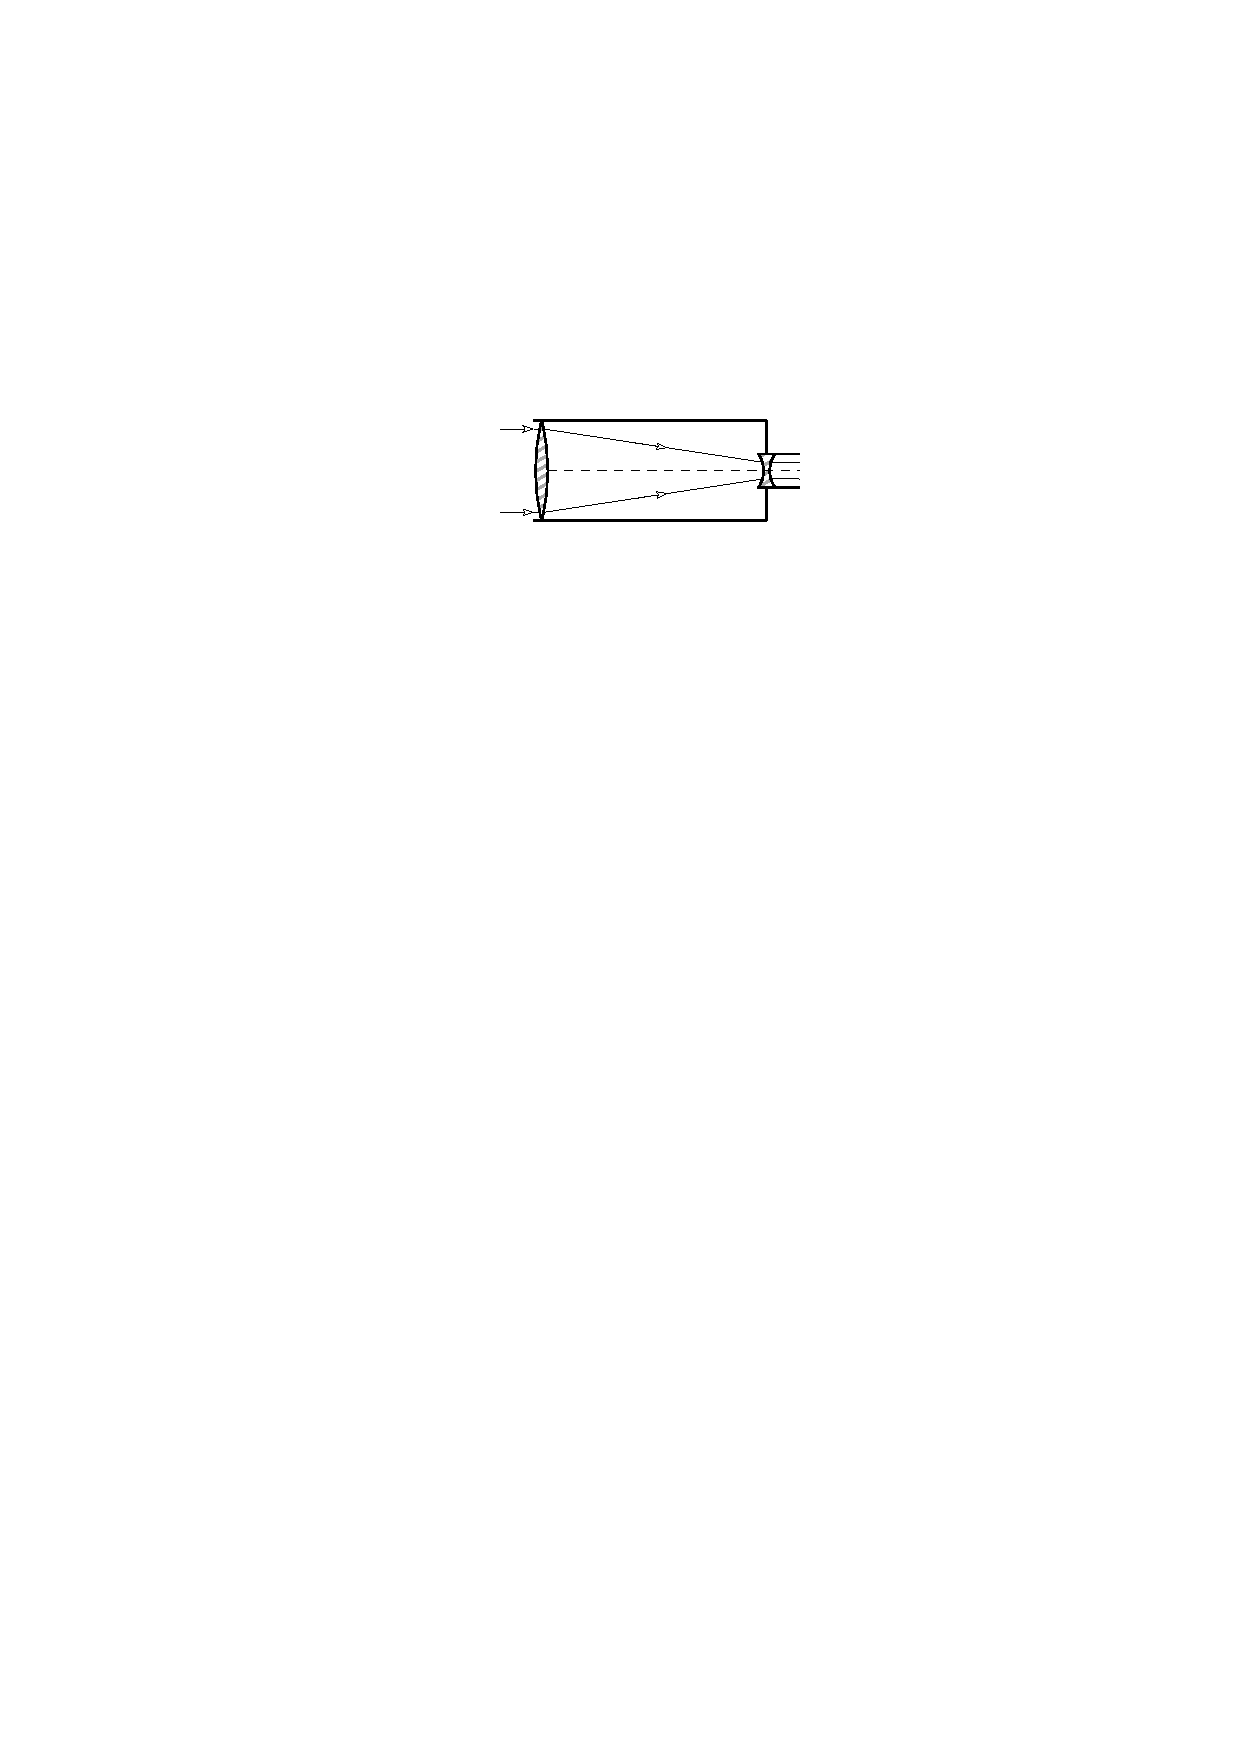
\includegraphics[width = \tw]{Galiley}
        \caption{Рефрактор системы Галилея}
    \end{subcaptionblock}
    \hfill
    \begin{subcaptionblock}{0.49\tw}
        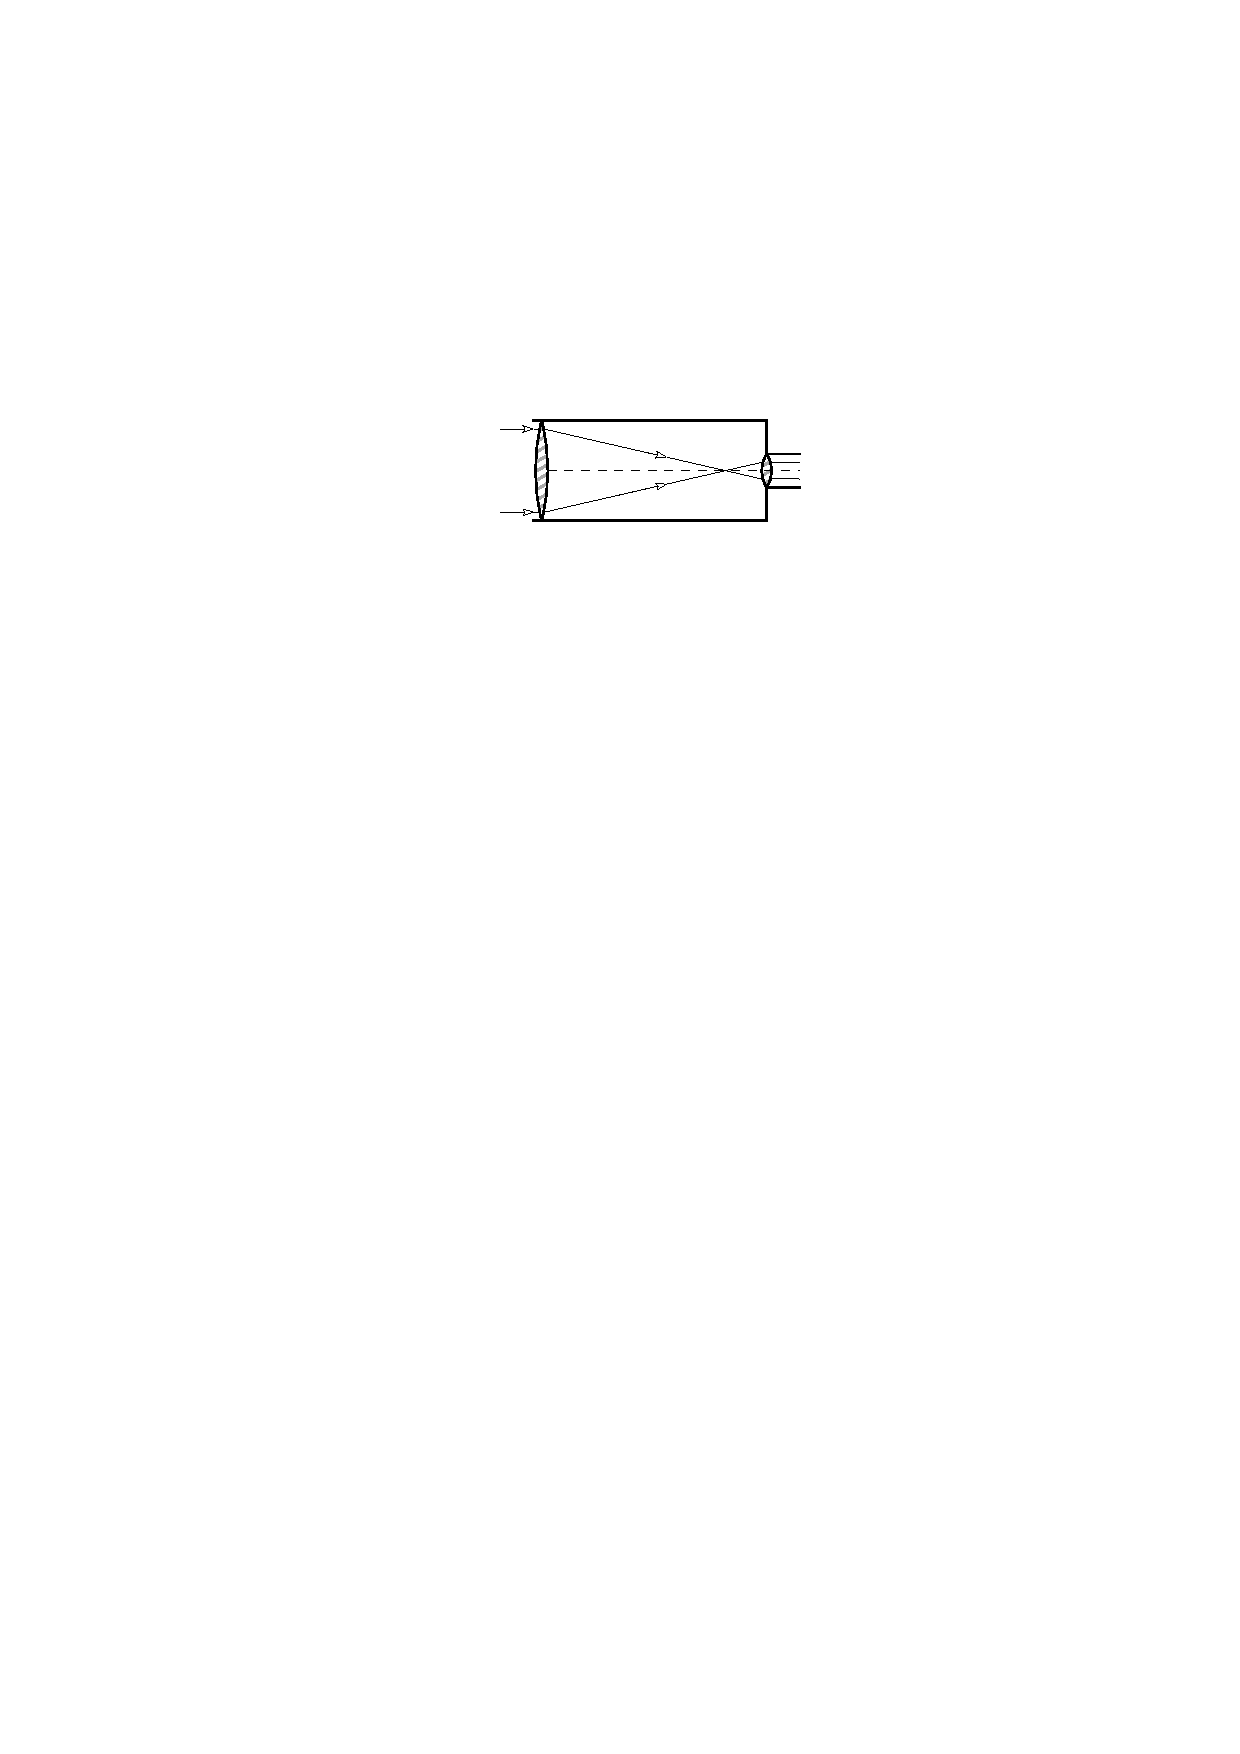
\includegraphics[width = \tw]{Kepler}
        \caption{Рефрактор системы Кеплера}
        \label{Kepler}
    \end{subcaptionblock}
    \caption{Оптические схемы телескопов рефракторов}
\end{figure}

\imp{Система Галилея}~--- окуляр является рассеивающей линзой и располагается перед фокусом главной линзы, изображение прямое. И \imp{система Кеплера}~--- окуляром является положительная (собирающая) линза, находящаяся за главным фокусом, следовательно, телескоп такой схемы дает перевернутое изображение.

%\subsubsection*{Рефлектор} 
Оптический телескоп,  в котором светособирающими элементами являются зеркала называется \term{рефлектором} (\imp{зеркальным телескопом}). Апертура определяется диаметром главного зеркала. В силу удобства изготовления рефлекторов, они пользуются большой попопулярностью за счёт невысокой относительно рефракторов цены. Кроме того использование зеркал в оптической схеме позволяет сильно её разнообразить. Зеркально-линзовый телескоп называется \term{катадиоптрическим}~--- телескоп, в котором используется как система линз, так и зеркал. В обиходе часто не различают рефлекторы и катадиоптрики, обращая внимание лишь на тип главного собирающего элемента. 

\vspace{-.3pc}
\begin{figure}[h!]
    \begin{subcaptionblock}{0.49\tw}
        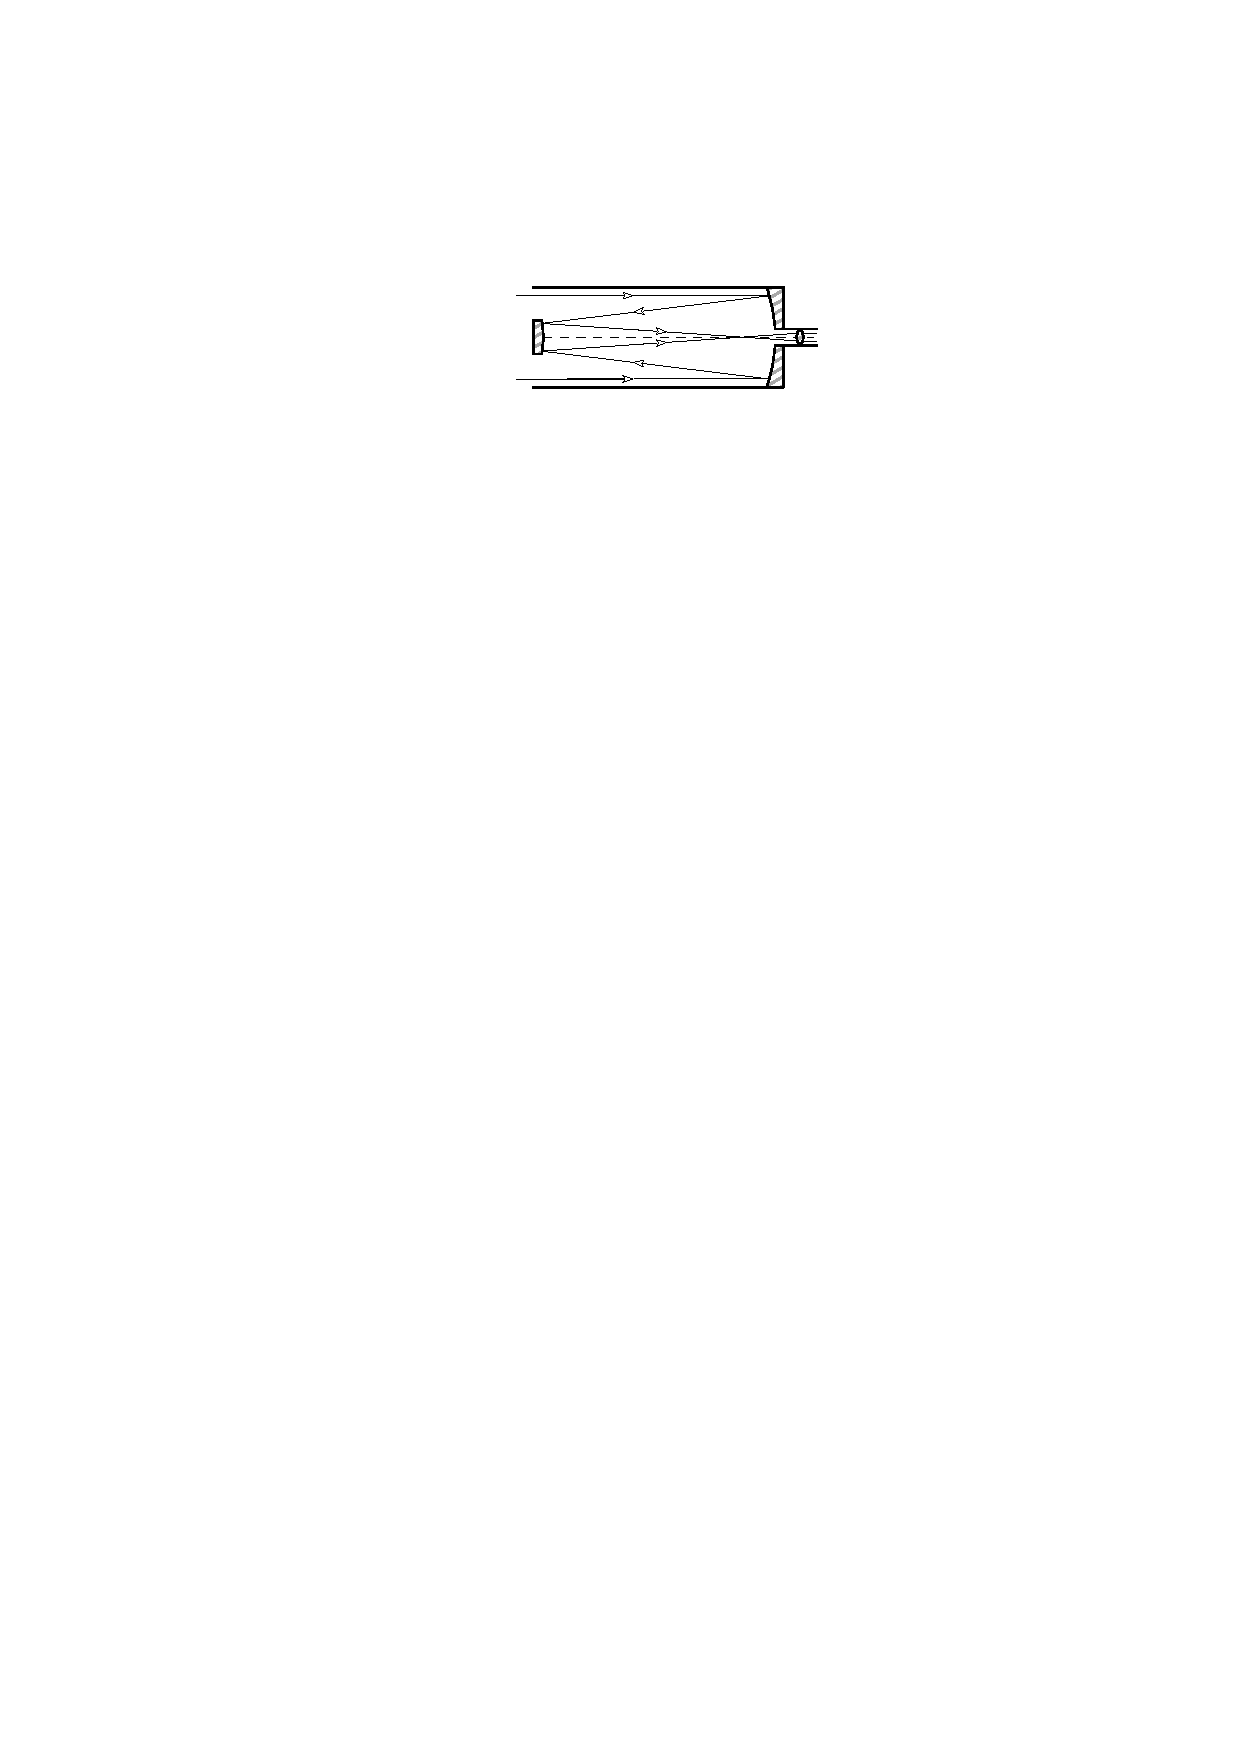
\includegraphics[width = \tw]{Cassigren.pdf}
        \caption{Рефлектор системы Кассегрена}
    \end{subcaptionblock}
    \hfill
    \begin{subcaptionblock}{0.49\tw}
        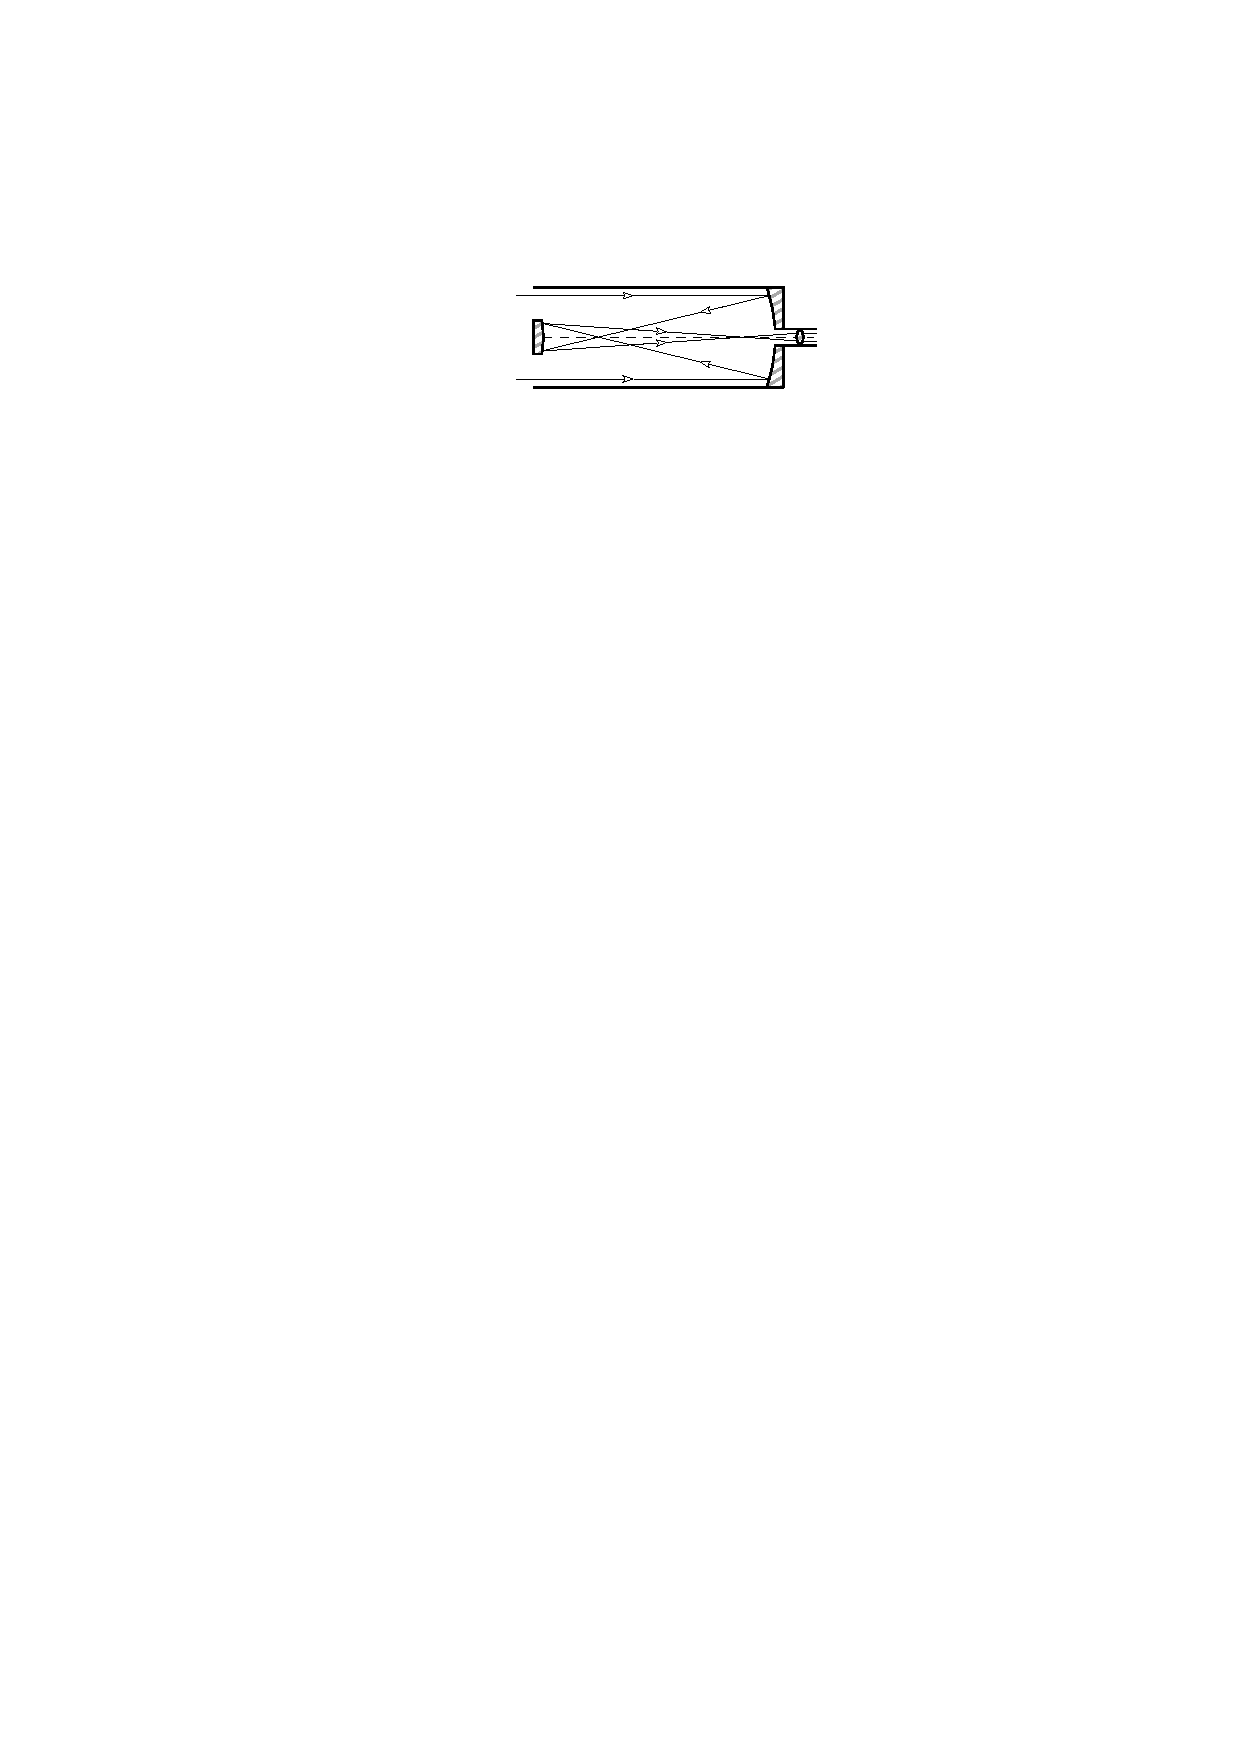
\includegraphics[width = \tw]{Gregory.pdf}
        \caption{Рефлектор системы Грегори}
        \label{Gregory}
    \end{subcaptionblock}
    \vskip4pt
    \begin{subcaptionblock}{0.49\tw}
        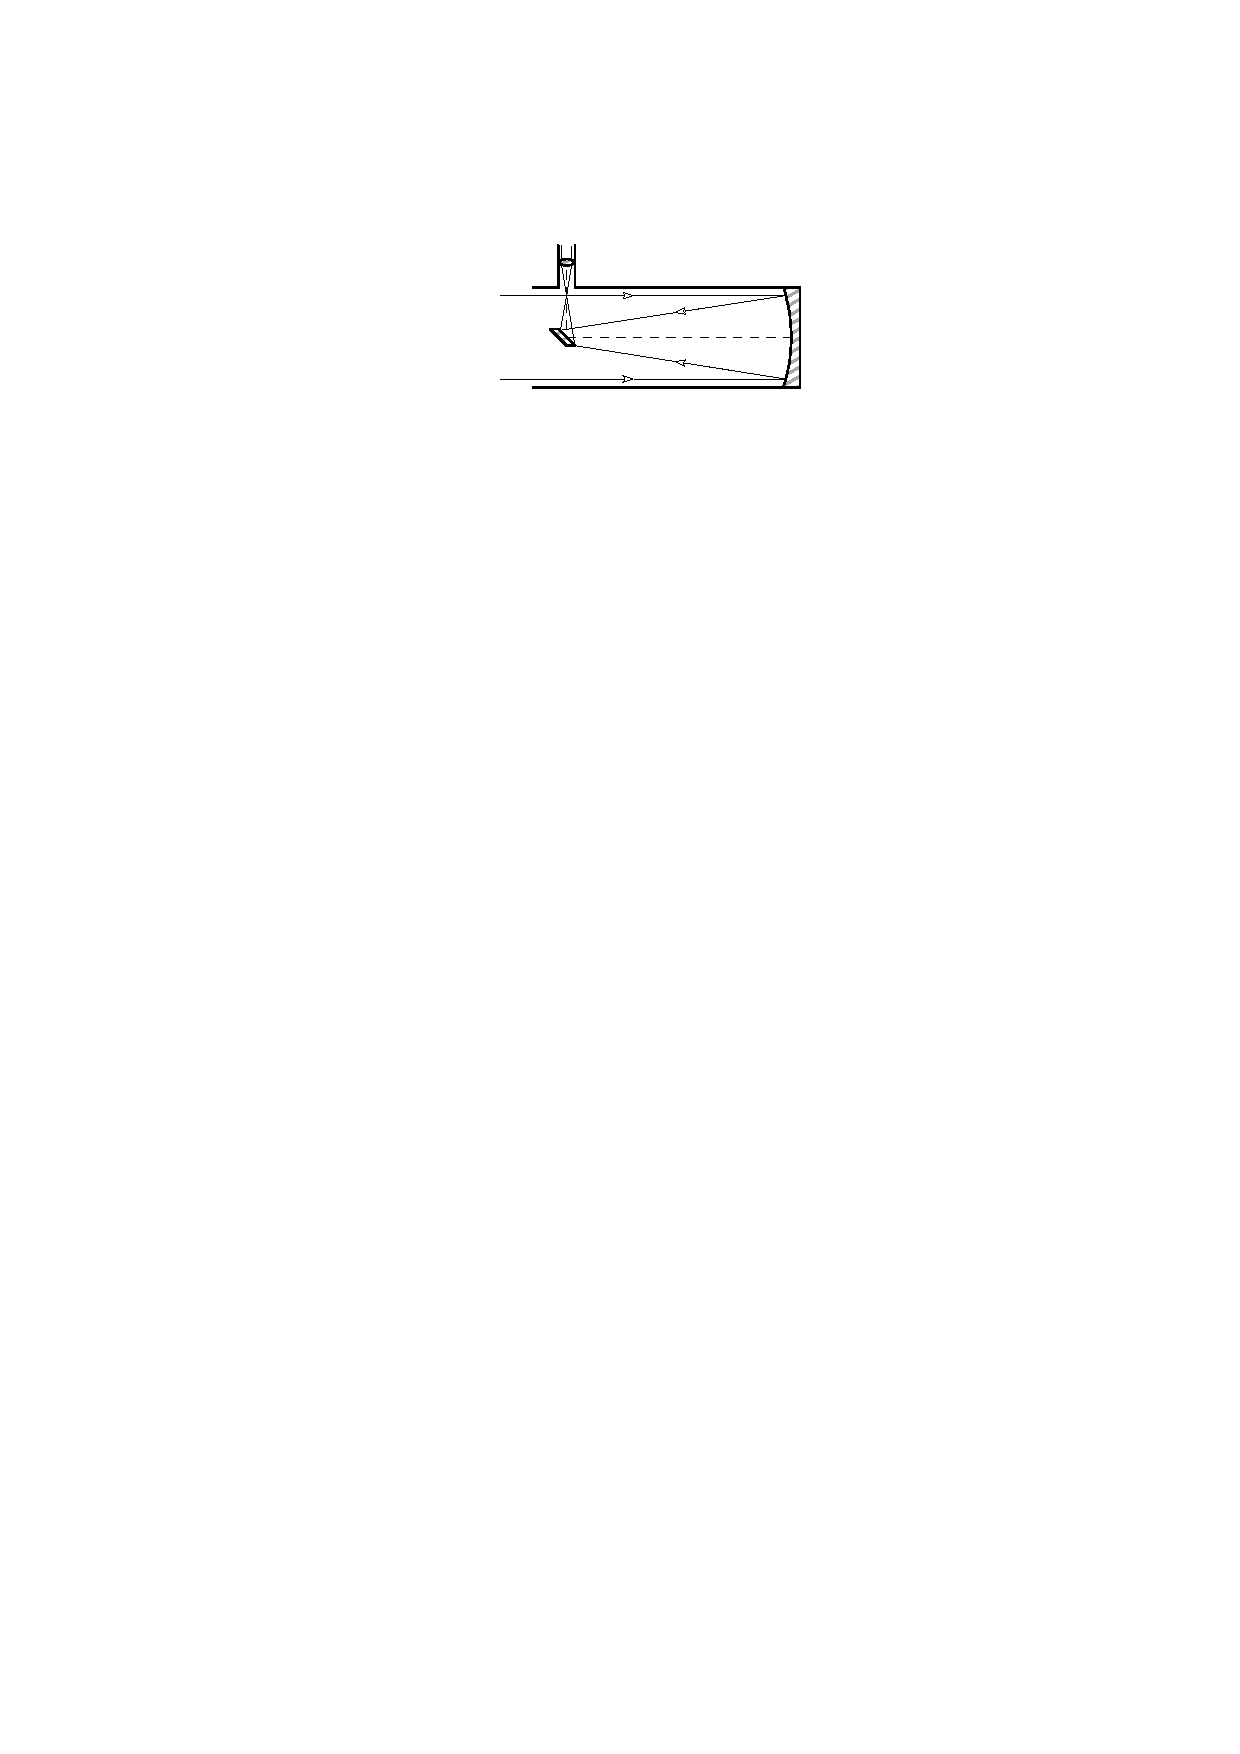
\includegraphics[width = \tw]{Newton}
        \caption{Рефлектор системы Ньютона}
    \end{subcaptionblock}
    \hfill
    \begin{subcaptionblock}{0.49\tw}
        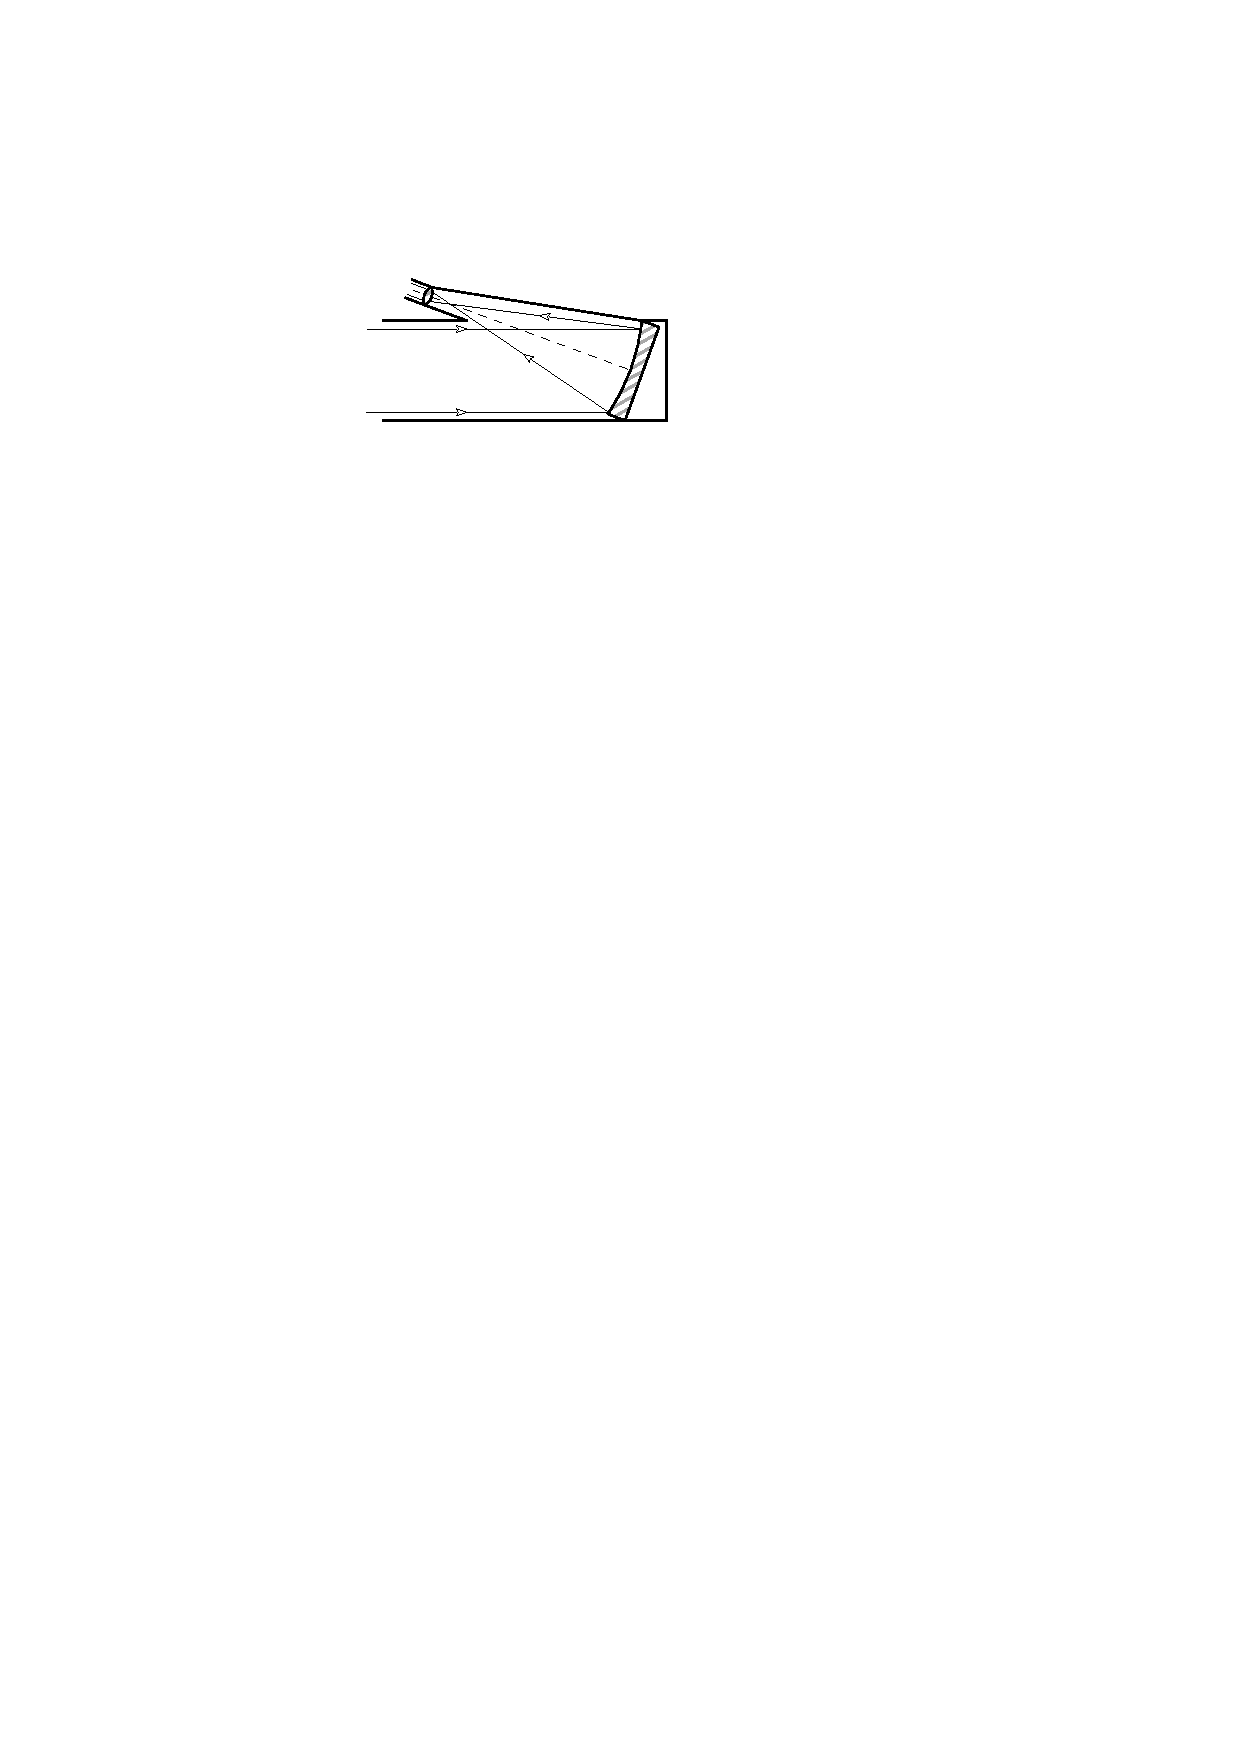
\includegraphics[width = \tw]{Lomonosov.pdf}
        \caption{Рефлектор системы Ломоносова}
    \end{subcaptionblock}
    \caption{Оптические схемы телескопов рефлекторов}
\end{figure}

Первый телескоп телескоп-рефлектор был построен Ньютоном по его же схеме в 1668 году. Главное зеркало параболическое, вторичное~--- плоское, наклонено под $45^\circ$ к оптической оси. Вторичное зеркало в схеме Ньютона поворачивает оптическую ось и выносит фокус из трубы. Изображение получается перевернутым, так как окуляр, как и для все телескопов рефлекторов, являясь собирающей линзой, располагается за фокусом.

Несмотря та то, что Ньютон построил первый телескоп-рефлектор, первую схему телескопа предложим не он, а Грегори, и сделал он это в 1663 году. В его схеме все зеркала расположены соосно, главное~--- параболическое, вторичное~--- эллиптическое. Первый главный фокус в системе Грегори расположен до вторичного зеркала, именно это и позволяет использовать эллиптическое зеркало в качестве вторичного. После вторичного зеркала находится второго главный фокус, а значит, телескоп с такой схемой строит прямое изображение.

В 1672 году Кассегрен предложил модификацию системы Грегори. В качестве вторичного зеркала он предложил использовать выпуклое гиперболическое, вместо вогнутого эллиптического, как было в Грегори. Это позволяет избавиться от второго главного фокуса и сократить размер трубы телескопа. А также такое вторичное зеркало приводит к меньшему экранированию главного, что улучшает проницающую способность. В последствие многие ученые модифицировали систему Кассегрена: добавляли различные апертурные корректоры, меняли форму зеркал. Самыми популярными, а потому и известными стали системы Максутова~--~Кассегрена, Шмидта~--~Кассегрена и Ричи~--~Кретьена.

Описанные выше схемы телескопов обладают важным недостатком: вторичное зеркало затеняет центральную область главного зеркала, причём чем больше относительное отверстие, тем больше затеняемая площадь. В 1762 году М.\,В.~Ломоносов реализовал схему телескопа-реф\-лек\-тора без вторичного зеркала. Главное зеркало в его схеме~--- внеосевой параболоид, фокус которого находится за пределами трубы. К сожалению данная оптическая схема не получила распространения из-за сильной комы.



\subsection{Виньетирование}
\imp{Виньетирование} (от франц. vignette~--- заставка), явление частичного ограничения (затенения) различными диафрагмами оптической системы наклонных (по отношению к оптической оси) пучков световых лучей.\footnote{{\itshape Фото и кинотехника}: <<Советская энциклопедия>>, 1981.}

В однолинзовых рефракторах перекрытия световых пучков не происходит, однако виньетирование наблюдается. Связано это с изменение эффективной площадью $S'$ собирающей поверхности в зависимости от угла $\alpha$ между центральным лучом пучка и оптической осью. Пусть площадь линзы равна $S$, тогда $S' = S\cos \alpha$. Отсюда получаем зависимость яркости изображения от линейного расстояния $x$ от оптическое оси в фокальной плоскости:
\begin{equation*}
	\frac{I}{I_0} = \cos \frac{x}{F},
\end{equation*}
где $F$~---  фокусное расстояние линзы, а $I_0$~--- яркость на оптической оси.

Однако в телескопах-рефракторах этот эффект ничтожно мал в силу малости поля зрения, а значит, и угла $\alpha$. Так как при $\alpha \ll 1$ с хорошей точностью справедливо приближение $\cos \alpha \simeq 1$. С другой стороны виньетирование сильно проявляется в широкоугольных объективах, угол $\alpha$ там может быть вплоть до $90^\circ$. Поэтому, но не только, фотографические объективы состоят из большого числа линз.


\subsection{Монтировки телескопов}
Монтировки телескопов разделяют на два основных вида: \imp{экваториальная} и \imp{альтзимутальная} монтировка (см.~Рис.\,\ref{mounts}).
\begin{figure}[h]
	\centering
	\hspace*{.4cm}
	\begin{subcaptionblock}{0.48\textwidth}
		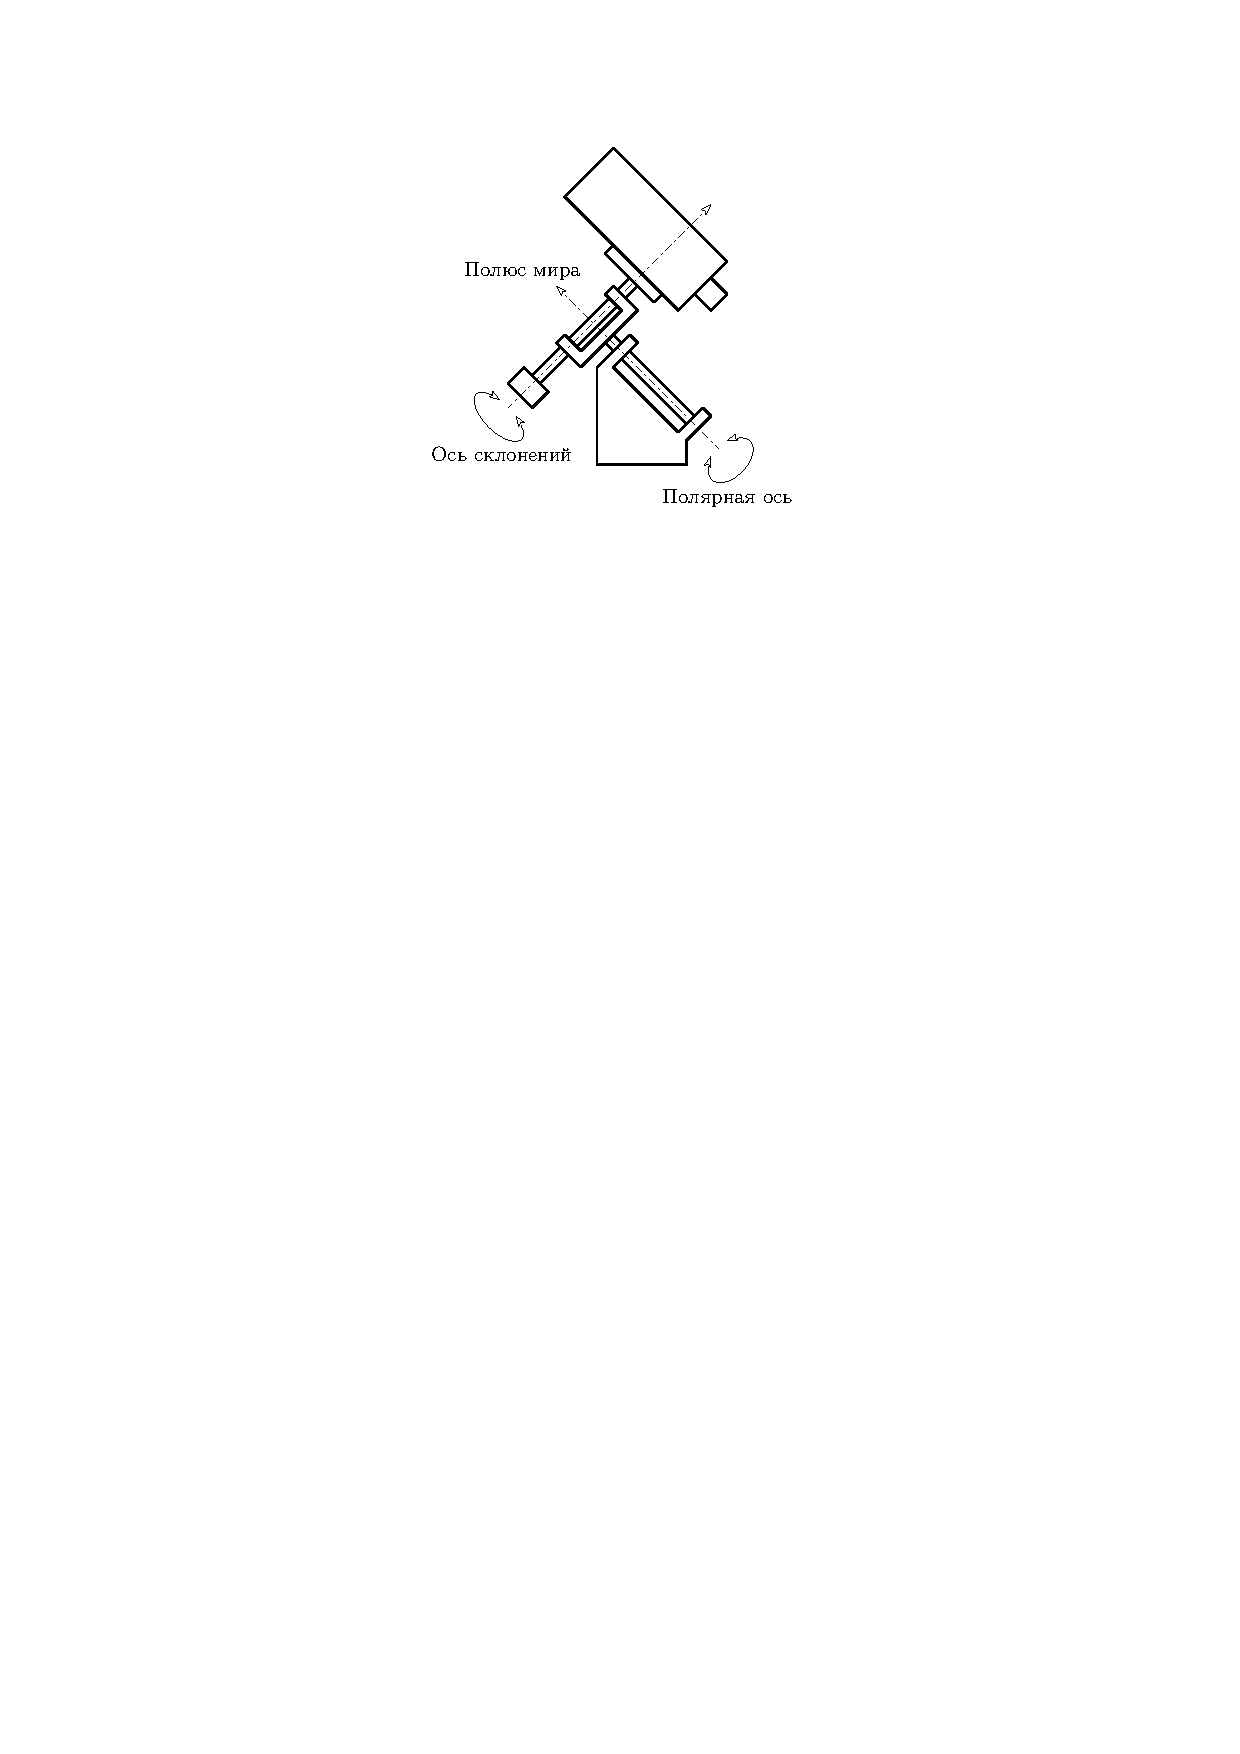
\includegraphics[height = 5cm]{mount-eq}
		\caption{Экваториальная мортировка}
	\end{subcaptionblock}
	\hspace*{.4cm}
	\begin{subcaptionblock}{0.41\textwidth}
		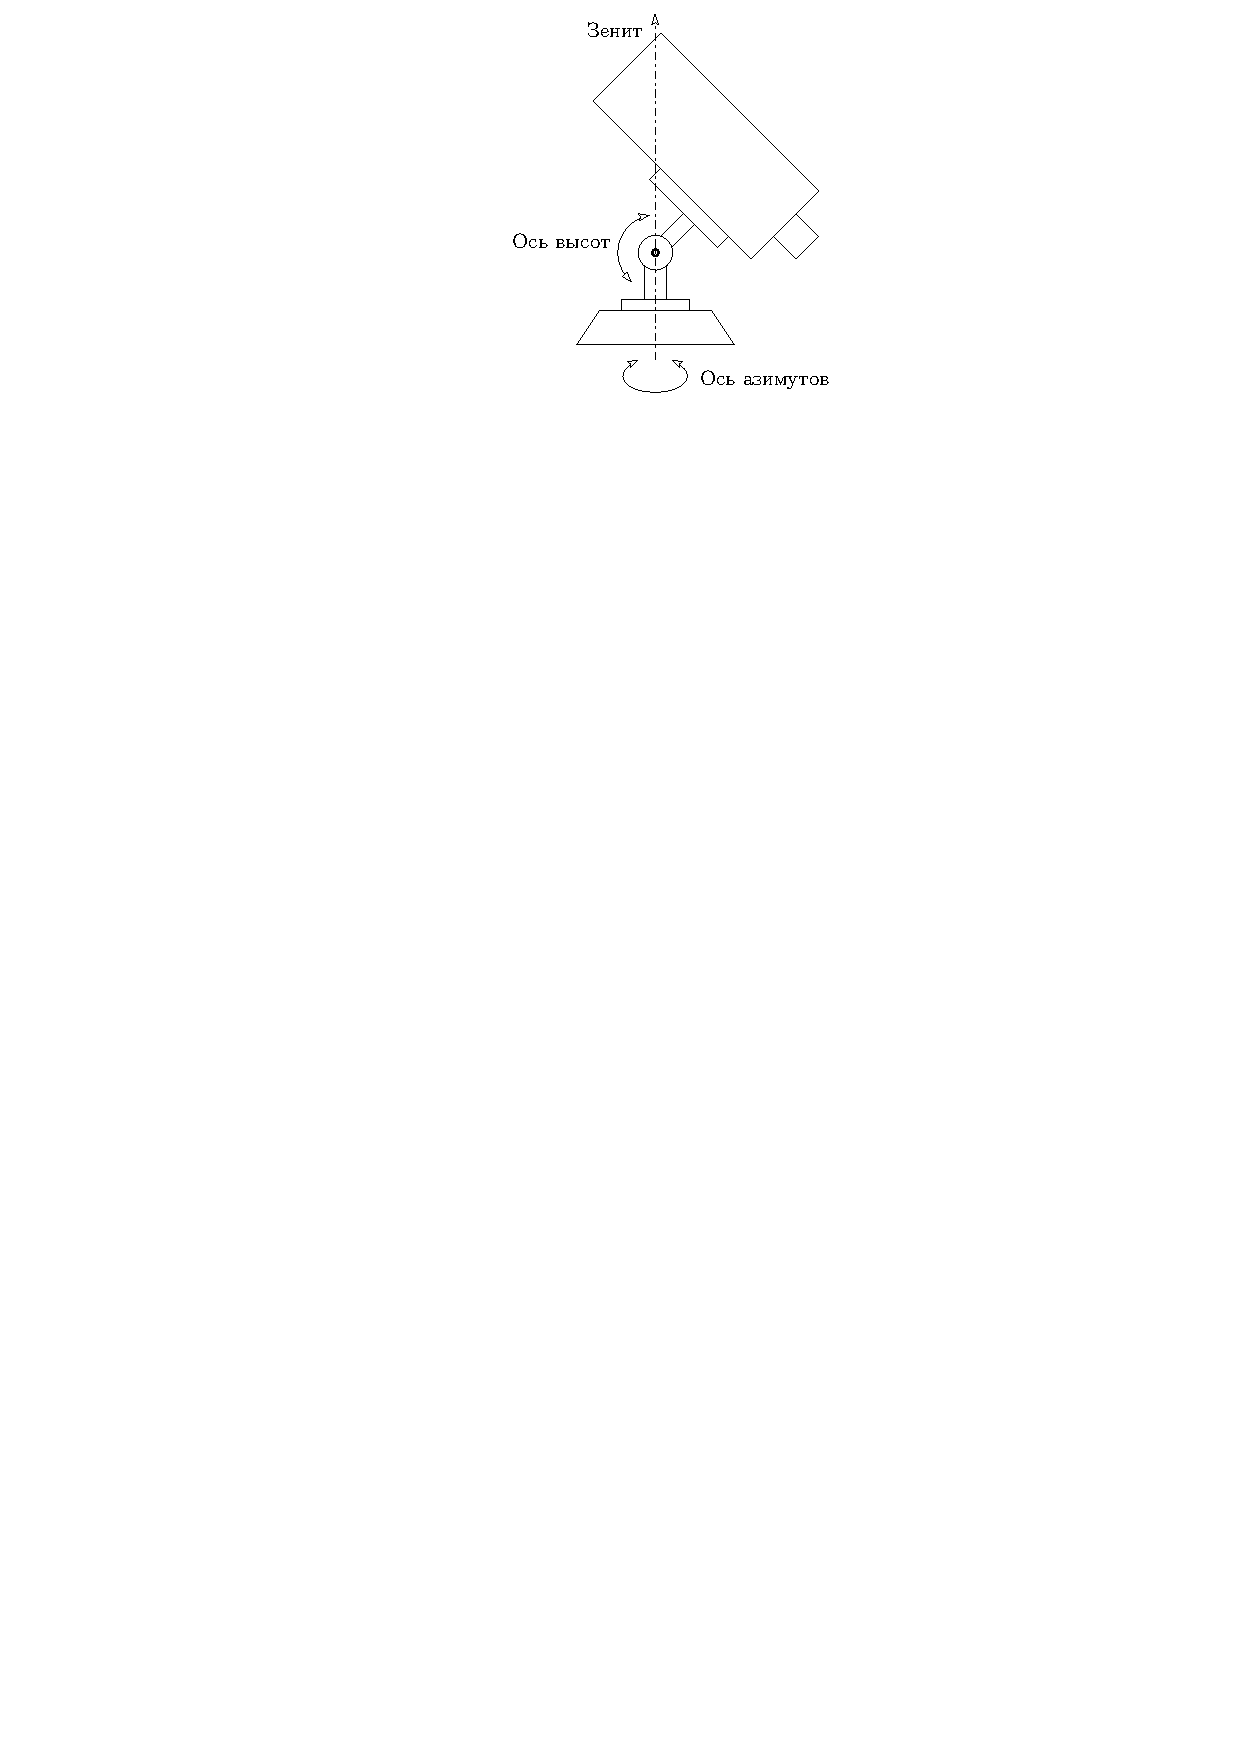
\includegraphics[height = 5cm]{mount-alt}
		\caption{Альтзимутальная монтировка}
	\end{subcaptionblock}
	\hspace*{.4cm}
	\caption{Виды монтировок}
	\label{mounts}
\end{figure}

\term{Экваториальная монтировка}~--- монтировка, одна ось которой направлена на полюс мира (полярная ось), а другая параллельна небесному экватору (ось склонения).
Для гидирования на такой монтировке, нужно лишь поворачивать её с постоянной угловой скоростью вокруг полярной оси в направлении роста часового угла.
Важно отметить, что существует несколько разновидностей экваториальных монтировок: \imp{немецкая}, \imp{английская}, \imp{американская} монтировки и монтировка \imp{с рамой}.

\term{Альтзимутальная монтировка}~--- монтировка телескопа, имеющая вертикальную и горизонтальную оси вращения, позволяющая поворачивать телескоп по высоте и по азимуту. Для слежения за небесными объектами, перемещающиеся по небесной сфере вследствие суточного вращения Земли, телескоп нужно поворачивать одновременно вокруг обеих осей с разными переменными скоростями.
\subsection{Параметры телескопа}
Из геометрической оптики известно, что лучи, проходящие через оптический центр линзы, не преломляются. Отсюда следует важное соотношение для линейного размера $l$ изображения объекта с угловым размером $\rho$ в фокальной плоскости:
\begin{equation}
	l = \rho F,
\end{equation}
здесь $F$~--- фокусное расстояние используемого телескопа.
Так как при помощи окуляра наблюдатель фактически смотрит на фокальную плоскость с расстояния $f$~--- фокусного расстояния окуляра, то угловой размер изображения, которое видит наблюдатель равно
\begin{equation}
	\alpha = \frac{l}{f}.
	\label{eq:zoom2}
\end{equation}
Следовательно, \term{увеличение телескопа}~$\Gamma$~--- отношение наблюдаемого и реального угловых размеров объекта равно отношению фокусных расстояний телескопа и окуляра. Из подобных треугольников также следует, что
\begin{equation}
	\Gamma =\frac{F}{f} = \frac{D}{d},
	\label{eq:zoom1}
\end{equation}
где $D$~--- диаметр входного зрачка (телескопа), $d$~--- диаметр выходного зрачка (окуляра). Важно отметить, что диаметры выходного и входного зрачка~--- диаметры пучков света, а не самих линз.

Увеличение называется \imp{равнозрачковым}, если диаметр выходного зрачка равен диаметру глазного зрачка наблюдателя, то есть
\begin{equation}
	\Gamma_\text{р.з.} = \frac{D}{d_\text{г}},
\end{equation}
где $d_\text{г}$~--- диаметр человеческого зрачка, обычно в тёмное время суток принимается за~6~мм.

Однако при росте увеличения детальность наблюдаемого изображения не улучшается. Происходит это в силу волновой природы света и, как следствие, явления \imp{дифракции} на входном отверстии телескопа. Наименьший угловой размер ещё различимых деталей определяется \term{разрешающей способностью} телескопа~--- это наименьшее угловое расстояние между двумя точечными объектами, при котором в телескоп ещё можно различить их раздельно. Предельное разрешение телескопа определяется формулой
\begin{equation}
	\beta = \frac{1.22\lambda}{D},
\end{equation}
где $\lambda$ --- длина волны наблюдений, при визуальных наблюдениях $\lambda \approx 550$~нм.

Кроме того, чем больше увеличение, тем меньше \term{поле зрения}~--- множество направлений, доступных для наблюдения. Из соотношений \eqref{eq:zoom2} и \eqref{eq:zoom1} следует зависимость \imp{поле зрения телескопа} $\alpha_\text{т}$ от \imp{поля зрения окуляра} $\alpha_\text{ок}$:
\begin{equation}
	\alpha_\text{т} = \frac{\alpha_\text{ок}}{\text{Г}},
\end{equation}
поле зрения стандартного окуляра составляет $45^\circ$.

Также, поле зрения телескопа можно вычислить, зная время $\tau$, за которое звезда со склонением $\delta$ пересекает поле зрения через его центр:
\begin{equation}
	\alpha_\text{т} = \frac{\tau \cos\delta}{4}.
\end{equation}

\term{Масштаб}~--- отношение углового размера объекта к линейному размеру его изображения на фокальной плоскости, следовательно
\begin{equation}
	\mu = \frac{\rho}{l} = \frac{\rho}{\rho F} = \frac{1}{F}=\left[\frac{\text{рад}}{\text{м}}\right].
\end{equation}

\term{Относительное отверстие}~--- геометрический параметр телескопа, равный отношению диаметра телескопа к его фокусному расстоянию
\begin{equation}
	\forall=\frac{D}{F}.
\end{equation}

\term{Светосила}~--- отношение освещенностей входного отверстия и фокальной плоскости, равна квадрату относительного отверстия.
\begin{equation}
	A=\forall^2=\frac{D^2}{F^2}.
\end{equation}

Пожалуй, самой важной характеристикой телескопа является то, насколько слабые объекты можно зафиксировать с его помощью. Эта величина называется \term{проницающей способностью телескопа}~--- это предельная звёздная величина объектов, которые доступны для наблюдения в данный телескоп. Чаще всего проницающая способность определяется из формулы Погсона \eqref{eq:pogson-law} в ходе сравнения телескопа с глазом ($m_\text{г} \simeq 6^m$), однако здесь нужно учесть:
\begin{enumerate}
	\item Отношение площадей собирающих поверхностей.
	\item Диаметр выходного пучка может быть больше размера приёмника, тогда часть света теряется.
	\item Отношение времён экспозиций (выдержка глаза составляет около 0.3~сек).
	\item Отношение квантовых эффективностей\footnote{\term{Квантовая эффективность}~--- отношение мощности регистрируемого излучения к мощности подающего для единицы площади приемника.}.
	\item Прочие эффекты, возникающие в ходе фотографических наблюдений.
\end{enumerate}
При учёте только первых двух пунктов проницающая способность равна
\begin{equation}
	m_\text{т} = m_\text{г} + 5\lg\frac{D}{d_\text{г}} - 5\lg\max \left\{ \frac{d}{d_\text{г}}, 1\right\}.
\end{equation}

\subsection{Формула тонкой линзы}

\begin{wrapfigure}[9]{c}{0.6\tw}
    \centering
    \vspace{-1pc}
    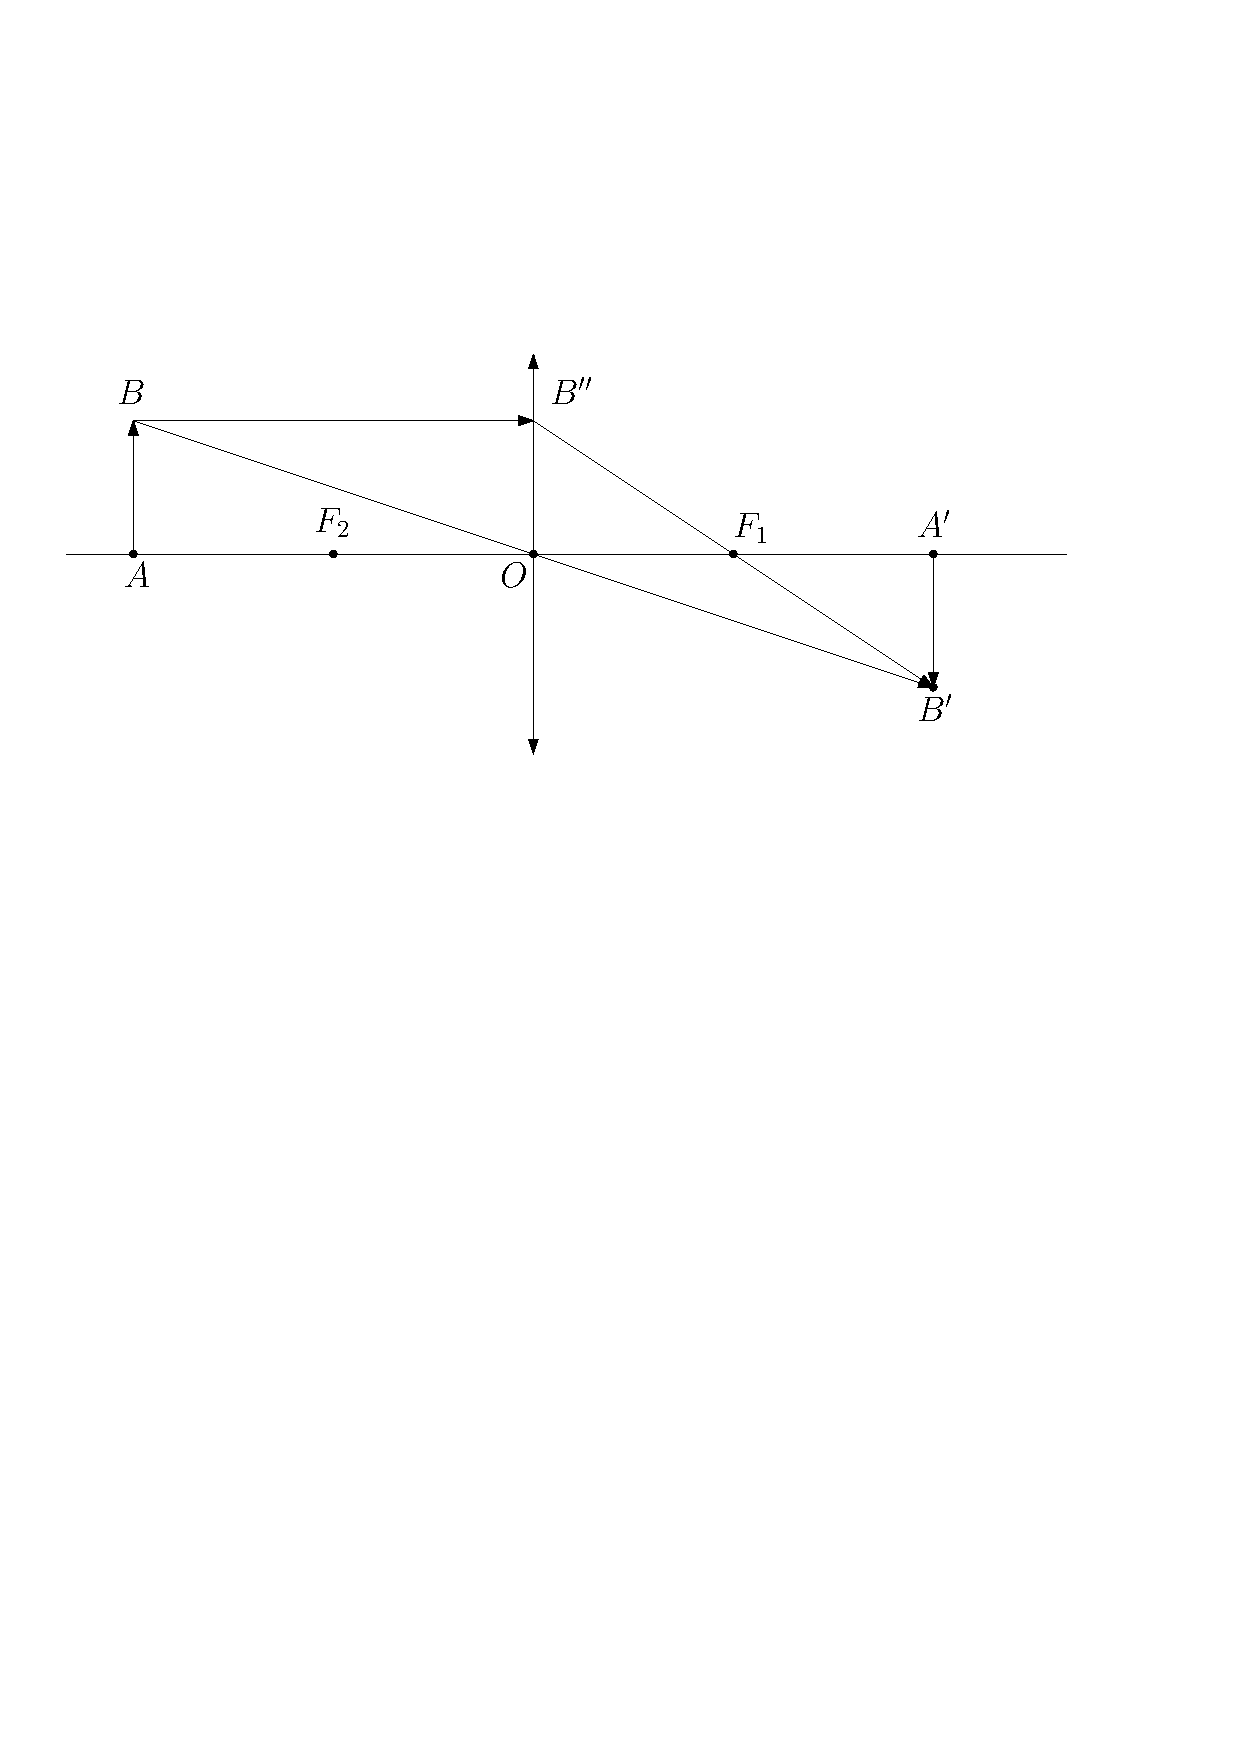
\includegraphics[width=.6\tw]{thin-lense}
    \caption{Схема лучей в тонкой линзе}
    \label{fig:thin-lens}
\end{wrapfigure}

Выведем формулу для связи расстояния от объекта до линзы, расстояния до изображения и фокусным расстоянием линзы.
Введем обозначения: $F = OF_1 = OF_2$~--- фокусное расстояние линзы, $d = OA = BB^{\prime \prime}$~--- расстояние до объекта, $f = OA^\prime$~--- расстоние до изображения.
\begin{equation}
    \Delta ABO \sim \Delta A^\prime B^\prime O \Longrightarrow \frac{d}{f} = \frac{OB}{OB^\prime} = \frac{AB}{A^\prime B^\prime}
\end{equation}
\begin{equation}
    \Delta OB^{\prime \prime} F_1 \sim \Delta A^\prime B^\prime F_1 \Longrightarrow \frac{f - F}{F} = \frac{F_1 B^\prime}{OF_1} = \frac{A^\prime B^\prime}{OB^{\prime \prime}} = \frac{A^\prime B^\prime}{AB}
\end{equation}
\begin{equation}
    \frac{f}{d} = \frac{f - F}{F} \Longrightarrow \frac{1}{d} = \frac{1}{F} - \frac{1}{f} \Longrightarrow \frac{1}{F} = \frac{1}{f} + \frac{1}{d}
\end{equation}
Полученная формула называется формулой тонкой линзой.


\subsection{Закон Снеллиуса}
Рассмотрим плоскую \imp{границу раздела} двух сред и луч, падающий на нее. Прямая, нормальная к плоскости раздела и проходящая через точку падения называется \imp{нормалью}. \term{Угол падение}~--- угол между нормалью и падающим лучем. В общем случае часть падающего излучения отражается от границы раздела, а часть проходит во вторую среду. \term{Углом отражения} называется угол между нормалью и отраженным лучем, а \term{углом преломления}~--- угол между нормалью и преломленным лучем.

Оптически прозрачная среда характеризуется скоростью распространения электромагнитного излучения (скоростью света) в ней. Скорость света в прозрачной среде определяется как
\begin{equation}
	c = \frac{c_0}{n},
\end{equation}
где $c_0$~--- скорость света в вакууме, а $n$~--- коэффициент преломления среды.

\term{Преломление}~--- изменение направления распространения волн (лучей) электромагнитного излучения, возникающее на границе раздела двух прозрачных для этих волн сред. Преломление света на границе двух сред даёт парадоксальный зрительный эффект: пересекающие границу раздела прямые предметы в более плотной среде ($n_1 >  n_2$) выглядят образующими больший угол с нормалью к границе раздела (то есть преломлёнными <<вверх»>>); в то время как луч, входящий в более плотную среду, распространяется в ней под меньшим углом к нормали (то есть преломляется <<вниз>>). Этот же оптический эффект приводит к ошибкам в визуальном определении глубины водоёма, которая всегда кажется меньше, чем есть на самом деле.

\begin{wrapfigure}[11]{r}{0.45\tw}
	\centering
	\vspace{-1pc}
	\begin{tikzpicture}
		\footnotesize
		
		\coordinate (0) at (0, 0) {};
		\coordinate (A) at (1.5, 0.87) {};
		\coordinate (2) at (2, 0) {};
		\coordinate (B) at (.13, -.5) {};
		
		%		\tkzMarkRightAngle[size=.4](0, A, 2);
		%		\tkzMarkRightAngle[size=.4](0, B, 2);
		
		\draw [double, line cap = butt] (0, -.7) arc(-90:-75:.7);
		\draw [double, line cap = butt] (1.3, 0) arc(180:195:.7);
		\draw [line cap = butt] (.5, 0) arc(0:30:.5);
		\draw [line cap = butt] (0, .5) arc(90:120:.5);
		
		\draw [line width = .5pt] (-1.5, 0) -- (3, 0);
		
		\draw [dashes] (0, -2) -- (0, 2);
		
		\draw [line width = 1pt] (-1.15, 2) -- (0, 0);
		\draw [line width = 1pt] (0.85, 2) -- (2, 0);
		\draw [line width = 1pt] (0.54, -2) -- (0, 0);
		\draw [line width = 1pt] (2.54, -2) -- (2, 0);
		\draw [line width = 1pt, -latex] (-1.15, 2) -- (-0.57, 1);
		\draw [line width = 1pt, -latex] (0.85, 2) -- (1.43, 1);
		\draw [line width = 1pt, -latex] (0, 0) -- (0.27, -1);
		\draw [line width = 1pt, -latex] (2, 0) -- (2.27, -1) ;
		
		\draw (0) -- (A);
		\draw (B) -- (2);
		
		\draw (3, 0) node [anchor=south east] {$n_1$};
		\draw (3, 0) node [anchor=north east] {$n_2$};
		\draw (0, .5) node [anchor=south east] {$\alpha$};
		\draw (.5, 0) node [anchor=south west] {$\alpha$};
		\draw (-.05, -.9) node [anchor=north west] {$\beta$};
		\draw (1, .06) node [anchor=north east] {$\beta$};
		
		вв	\end{tikzpicture}
		\caption{Ход лучей при прохождении границы раздела двух сред ввнаправлении из оптически менее плотной в оптически более плотную среду}
		\label{}
	\end{wrapfigure}
	Преломление света в атмосфере Земли приводит к тому, что мы наблюдаем восход Солнца несколько раньше, а закат несколько позже, чем это имело бы место при отсутствии атмосферы. По той же причине вблизи горизонта диск Солнца выглядит заметно сплющенным вдоль вертикали.
	
	Закон преломления называется \term{законом Снеллиуса}. Оставим его без доказательства в силу необходимой для этого теории, выходящей за рамки данного книги. Формулируется закон Снеллиуса так:
	\begin{equation}
		n_1 \sin \alpha = n_2 \sin \beta,
		\label{eq:snell-law}
	\end{equation}
	где $\alpha$~--- угол между лучем и нормалью в среде 1, $\beta$~--- в среде 2.
	
	Из \eqref{eq:snell-law} видно, что для некоторых $n_1$ и $n_2$ таких, что, например $n_2 > n_1$, и достаточно большом угле $\beta$ должно выполняться неравенство $\sin \alpha > 1$, что, очевидно, невозможно. Данная ситуация называется \imp{полным внутренним отражением}~--- всё излучение, падающее из более оптически более плотной среды, отразится от границы раздела. \term{Углом полного внутреннего отражения} называется такой минимальный угол $\beta$, при котором наблюдается полное внутреннее отражение. Положив $\sin \alpha = 1$, получаем, что
	\begin{equation}
		\sin \beta_\text{min} = \frac{n_1}{n_2}, \quad n_1 < n_2.
	\end{equation}

\subsection{Аберрации в оптике}
\paragraph{Хроматическая аберрация}
Пожалуй главным недостатком оптических схем, содержащий преломляющие оптические элементы (линзы; призмы, за исключением использования их для спектроскопии) являются \imp{хроматические аберрации}. Дело в том, что показатель преломления материала линзы зависит от длины волны падающего излучения. Это приводит к тому, что положения фокуса оптической системы зависит от длины волны излучения. При наблюдениях это проявляется как радужный ореол вокруг объектов, ухудшающий качество изображения.

\begin{wrapfigure}{r}{0.5\tw}
	\centering
	\vspace{-1pc}
	\begin{tikzpicture}
		\begin{axis}[
			height	=	4.5cm,
			width	=	6cm,
			xlabel	=	{$\lambda$, мкм},
			ylabel	=	{$n(\lambda)$},
%			ylabel shift	= -1 cm,
			xmin = 0.3,
			xmax = 2.5,
			ymin = 1.48,
			ymax = 1.55,
			]
			
			\addplot[smooth, domain=0.3:2.5] table[x=l, y=n] {data/crown-dispersion.txt};
		\end{axis}
	\end{tikzpicture}
	\caption{}
	\label{pic:crown-dispersion}
\end{wrapfigure}
Найдем зависимость величины хроматической аберрации от величины дисперсии материала линзы. В качестве линзы рассмотрим плосковыпуклую линзу из оптического стекла~--- \imp{крона} (BK7). Зависимость $n(\lambda)$ её показателя преломления $n$ от длины волны $\lambda$ проходящего излучения представлена на графике (см.~Рис\,\ref{pic:crown-dispersion}). Важно отметить, здесь уже нельзя считать линзу тонкой, так как само по себе понятие тонкой линзы подразумевает отсутствие разного рода аберраций и условие фокусировки лучей в одной точке (фокусе), чего не происходит на практике.

\begin{wrapfigure}[9]{r}{0.63\tw}
	\centering
	\vspace{-.8pc}
	\begin{tikzpicture}
		\footnotesize
		
		\draw [decoration={snake, segment length=.7mm, amplitude=0.2mm}, decorate] (1.35, 1) arc(-31:15:0.26);
		\draw [double, line cap=butt] (.2, 1.135) arc(180:195:0.94);
		\draw  (2.7, 0) arc(180:149:0.3);
		
		\fill [lightgray] (.5, -1.5) -- (.5, 1.5) -- (1, 1.5) arc(20:-20:4.386) -- (.5, -1.5);
		
		\draw [thick] (.5, -1.5) -- (.5, 1.5);
		\draw [thick] (1, -1.5) arc(-20:20:4.386);
		\draw [semithick, dash pattern={on 5pt off 2pt on .5pt off 2pt}] (-3.8, 0) -- (3.2, 0);
		%		\draw (-3.12, 0) node{$\times$};
		
		\draw [dashes] (-3.12, 0) -- (1.71, 1.29);
		
		\draw [semithick] (-3.8, 1.135) -- (1.12, 1.135) -- (3, 0);
		\draw [-latex] (-3.5, 1.135)-- (-1, 1.135);
		\draw [-latex] (1.12, 1.135) -- (2.25, 0.45);
		
		\draw [latex-latex] (-3.5, 0) -- (-3.5, 1.135);
		\draw [latex-latex] (1.27, -.5) -- (3, -.5);
		\draw [latex-latex] (1.12, -1.4) -- (3, -1.4);
		\draw [-latex] (0.5, -.5) -- (1.12, -.5);
		
		\draw (1.12, 1.135) -- (1.12, -1.5);
		\draw (1.27, 0) -- (1.27, -.6);
		\draw (3, 0) -- (3, -1.5);
		
		\draw (-3.5, 0.56) node[anchor=east] {$d$};
		\draw (-3.12, 0) node[anchor=north] {$C$};
		\draw (-.7, 0.6) node[anchor=north] {$R$};
		\draw (2.14, -.5) node[anchor=south] {$x$};
		\draw (2.14, -1.4) node[anchor=south] {$\frac{d}{\tg \gamma}$};
		
		\draw (.8, -1.5) node[anchor=south] {$n$};
		
		\draw (.2, 1) node[anchor=east] {$\alpha$};
		\draw (1.4, 1.07) node[anchor=west] {$\beta$};
		\draw (2.65, 0.15) node[anchor=east] {$\gamma$};
		
		\draw [fill=white] (3, 0) circle (.03);
		\draw [fill=white] (-3.12, 0) circle (.03);
	\end{tikzpicture}
	\caption{}
	\label{pic:sphere-aberrations-lens}
\end{wrapfigure}
Итак, пусть радиус кривизны выпуклой поверхности рассматриваемой плос\-ко-вы\-пук\-лой линзы равен $R$. Рассмотрим также луч, параллельный оптической оси данной линзы, на расстоянии $d$ от этой оси (см.~Рис.\,\ref{pic:sphere-aberrations-lens}). Так как передняя поверхность линзы плоская, луч, попадая в линзу, не преломляется. Преломление происходит на выходе из линзы. Нетрудно показать, что для угла падения луча на заднюю поверхность линзы $\alpha$ справедливо, что $\sin \alpha = d/R$. По закону Снеллиуса угол преломления рассматримоего луча $\beta$ определяется соотношением $\sin \beta = n \sin \alpha$. Так как угол между нормалью к выпуклой поверхности линзы и ее оптической осью равен $\alpha$, то угол $\gamma$ между преломленным лучем и оптической осью линзы равен $\beta - \alpha$.

Расстояние до точки пересечения преломлённого луча с оптической осью линзы будем отсчитывать от вершины выпуклой поверхности линзы. Расстояние $h$ между проекцией точки преломления на оптическую ось и вершиной можно найти из теоремы Пифагора:
\begin{equation*}
	h = R - \sqrt{R^2 - d^2}.
\end{equation*}
Тогда координата фокуса для лучей на расстоянии $d$ от оптической оси равно
\begin{equation}
	x = \frac{d}{\tg \gamma} - h = \frac{d}{\tg \left( \arcsin \dfrac{n d}{R} - \arcsin \dfrac{d}{R} \right)} - \left( R - \sqrt{R^2 - d^2} \right).
	\label{eq:optics-aberr-x(d)}
\end{equation}
Введём обозначение $\delta \equiv d/R$ и разделим обе части полученного равенства на $R$, чтобы перейти к относительным единицам:
\begin{equation}
	\frac{x}{R}
	= \frac{\delta}{\tg \left( \arcsin n\delta - \arcsin \delta \right)} -  1 + \sqrt{1 - \delta^2}
	~\xrightarrow{\delta \ll 1}~  \frac{1}{n - 1} - \frac{\delta^2 n^2}{2(n-1)}.\footnote{\scriptsize Вывод приближения:
	\begin{multline*}
		\frac{\delta}{\tg \left( \arcsin n\delta - \arcsin \delta \right)} -  1 + \sqrt{1 - \delta^2} =\\
		= \frac{\delta}{\tg \left[ n \delta + \dfrac{n^3 \delta^3}{6} - \delta - \dfrac{ \delta^3}{6} + o(\delta^3) \right]} -  1 + \left(1 - \frac{\delta^2}{2} + o(\delta^2) \right) =\\
		= \frac{\delta}{\tg \left[ \delta(n-1) + \dfrac{(n^3-1) \delta^3}{6} + o(\delta^3) \right]} - \frac{\delta^2}{2} + o(\delta^2) =\\
		= \frac{\delta}{\delta(n-1) + \dfrac{(n^3-1) \delta^3}{6} + \dfrac{\delta^3}{3}(n-1)^3 + o(\delta^3)} - \frac{\delta^2}{2} + o(\delta^2) =\\
		= \frac{1/(n-1)}{1 + \dfrac{\delta^2}{6}(n^2 + n + 1) + \dfrac{\delta^2}{3}(n-1)^2 + o(\delta^2)} - \frac{\delta^2}{2} + o(\delta^2) =\\
		=\frac{1}{n-1} \left[1 - \frac{\delta^2}{6} (3n^2 -3n + 3) \right] - \frac{\delta^2}{2} + o(\delta^2)
		%	= \frac{1}{n-1} - \frac{\delta^2}{2(n-1)}(n^2 - n + 1 + n - 1) + o(\delta^2)
		\simeq \frac{1}{n-1} - \frac{\delta^2 n^2}{2(n-1)}.
	\end{multline*}
	}
\end{equation}

Найдём область определения функции $x(\delta)$. Прежде всего $\delta \geqslant 0$, потому что $d$~--- это расстояние от оптической оси, которое не может быть отрицательным. С другой стороны радиус линзы не может быть больше радиуса кривизны ее поверхности, следовательно, $\delta < 1$. Однако есть ещё одно условие, которое ограничивает $\delta$ сверху. Это эффект полного внутреннего отражения. Действительно, $\sin \beta$ не может быть больше единицы, следовательно, $\sin \alpha < \sfrac{1}{n}$, а значит, $\delta < \sfrac{1}{n}$. Для стекла, коэффициент преломления которого $n \approx 1.5$, получаем, что $\delta \in [0, \sfrac{2}{3})$.

\begin{wrapfigure}{r}{0.5\tw}
	\centering
	\vspace{-1pc}
	\begin{tikzpicture}
		\begin{axis}[
			height	=	4.5cm,
			width	=	6cm,
			xlabel	=	{$\lambda$, мкм},
			ylabel	=	{$x(\lambda)$},
%			ylabel shift	= -1 cm,
			xmin = 0.3,
			xmax = 2.5,
			ymin = 1.8,
			ymax = 2.1,
			]
			
			\addplot[smooth, domain=0.3:2.5] table[x=l, y=x] {data/crown-dispersion.txt};
		\end{axis}
	\end{tikzpicture}
	\caption{}
	\label{pic:crown-dispersion-x}
\end{wrapfigure}
Как будет показано далее, во избежании проявления \imp{сферической аберрации}, используют линзы с маленьким относительным отверстием ($\forall \ll 1$). Следовательно, и $\delta \ll 1$, возьмем для примера значение $\delta = 0.1$. Для него, очевидно, можно использовать приближение для $x$, поэтому при заданном значении $\delta$ выражение для $x$ принимает вид:
\begin{equation*}
	x = \frac{1}{n-1} - \frac{0.01 n^2}{2(n-1)}.
\end{equation*}
Как видно из графика данной зависимости (см.~Рис.\,\ref{pic:crown-dispersion-x}), для оптического диапазона $x(\lambda)$ принимает значения от примерно 1.85 для коротковолновой (фиолетовой) части до примерно 1.95 для красного цвета.

Чтобы компенсировать такой разбег совместно с собирающей линзой использую рассеивающую из другого материала. Объективы, где исправлена хроматическая аберрация для двух цветов и частично исправлена сферическая аберрация называют \term{ахроматами}; где хроматическая аберрация исправлена для трёх цветов, а также полностью исправлена сферическая аберрация~--- \term{апохроматами}; с более полной геометрической коррекцией~--- \term{апланатами}.

\paragraph{Сферическая аберрация}
В оптических системах, содержащих \change{сферические поверхности (линзы, зеркала)} может наблюдаться \imp{сферическая аберрация}. Суть такой аберрации состоит в том, что лучи, параллельные оптической оси, идущие на разном расстоянии от неё собираются в разных её местах. Это приводит к тому, что изображения точечных источников размываются.

\begin{wrapfigure}[12]{r}{0.55\tw}
	\centering
	\vspace{-.5pc}
	\begin{tikzpicture}
		\begin{axis}[
			height	=	5cm,
			width	=	6.5cm,
			xlabel	=	{$\delta$},
			ylabel	=	{$x(\delta)/R$},
%			ylabel shift	= -1.1 cm,
			extra x ticks ={0.667},
			extra x tick labels={$\frac{1}{n}$},
			xmin=-.05,
			xmax=0.72,
			ymin=-.25,
			ymax=2.25,
			legend cell align=left,
			legend style={
			draw=none,
			fill=none,
			font=\scriptsize,
			at={(axis cs:0, 0.1)}, anchor=south west,
			row sep=.5pc,
			},
			]
			\addplot[smooth, gray] table[x=d, y=simple] {data/shere-aberrations-lens.txt};
			\addplot[smooth] table[x=d, y=x] {data/shere-aberrations-lens.txt};
			\addplot[dashes] coordinates { (0.667, -10) (0.667, 10)};
			\legend{
			$\left. \dfrac{x(\delta)}{R} \right|_{\delta \ll 1}$,
			$\dfrac{x(\delta)}{R}$,
			$\delta = \left.\dfrac{1}{n}\right|_{n=3/2}$,
			}
		\end{axis}
	\end{tikzpicture}
	\caption{}
	\label{pic:sphere-aberrations-lens-plot}
\end{wrapfigure}
Покажем наличие сферической аберрации для плосковыпуклой линзы. Рассмотрим полученное выше выражение \eqref{eq:optics-aberr-x(d)} и его приближение при $\delta \ll 1$. Зафиксируем в них $n=3/2$~--- характерное значение показателя преломления для стекла. Графики получаемых при этом зависимостей представлены на Рис.\,\ref{pic:sphere-aberrations-lens-plot}. Как видно из данных графиков, сферические аберрации проявляются уже на малых расстояниях от оптической оси.

Чтобы показать важность сферических аберраций рассмотрим небольшой телескоп рефрактор с диаметром плосковы\-пук\-ло\-во\-го\linebreak стеклянного ($n \approx 3/2$) объектива $D = 50$~мм. Характерная точность фокусировки $\Delta x$ для таких маленьких телескопов составляет около 1~мм. Установим, при каком фокусном расстоянии такого телескопа точность фокусировки нивелирует сферическую аберрацию.

При отсутствии сферической аберрации фокусное расстояние плосковыпуклового объектива $F = R/(n-1) = 2R$. Предельное значение $\delta$, которое нужно рассмотреть, соответствует лучам, проходящим через край объектива, следовательно, $\delta = D/(2R)$. Используя приближение, теперь можно записать выражение для требуемого $\Delta x$, чтобы найти необходимое для этого относительное отверситие $\forall$:
\begin{gather*}
	\Delta x = F - x(\delta) = F - x\left( \frac{D}{2R} \right),\\
	\Delta x = F - R\left( 2 - \frac{9 D^2}{4 \cdot 4R^2} \right),\\
	\Delta x = \frac{9D^2}{16R} = \frac{9D^2}{16F} = \frac{9}{16} D \forall;\\
	\therefore \forall = \frac{\Delta x \cdot 16}{9D} = 0.036.
\end{gather*}

\begin{wrapfigure}[9]{r}{0.5\tw}
	\centering
	\vspace{-.8pc}
	\begin{tikzpicture}
		\footnotesize
		
		\draw [decoration={snake, segment length=.7mm, amplitude=0.2mm}, decorate] (1.35, 1) arc(-31:15:0.26);
		\draw (.2, 1.135) arc(180:209:0.94);
		\draw (-2.18, 0) arc(0:15:0.94);
		
		\fill [lightgray] (1.5, -1.5) -- (1.5, 1.5) -- (1, 1.5) arc(20:-20:4.386) -- (1.5, -1.5);
		
		\draw [thick] (1, -1.5) arc(-20:20:4.386);
		\draw [semithick, dash pattern={on 5pt off 2pt on .5pt off 2pt}] (-3.8, 0) -- (1.7, 0);
		
		\draw [dashes] (-3.12, 0) -- (1.71, 1.29);
		
		\draw [semithick] (-3.8, 1.135) -- (1.12, 1.135) -- (-.85, 0);
		\draw [-latex] (-3.5, 1.135)-- (-1, 1.135);
		\draw [-latex] (1.12, 1.135) -- (-.06, 0.45);
		
		\draw [latex-latex] (-3.5, 0) -- (-3.5, 1.135);
		\draw [latex-latex] (-.85, -1.3) -- (1.27, -1.3);
		
		\draw (1.27, 0) -- (1.27, -1.5);
		\draw (-.85, 0) -- (-.85, -1.5);
		
		\draw (-3.5, 0.56) node[anchor=east] {$d$};
		\draw (-0.85, 0) node[anchor=north east] {$F$};
		\draw (-3.12, 0) node[anchor=south] {$C$};
		\draw (-1.2, 0.5) node[anchor=south] {$R$};
		\draw (0.27, -1.3) node[anchor=south] {$x_F(d)$};
		
		\draw (.2, 1) node[anchor=east] {$\alpha$};
		\draw (-2.2, .15) node[anchor=west] {$\alpha$};
		\draw (.3, .7) node[anchor=east] {$\alpha$};
		
		\draw [fill=white] (-0.85, 0) circle (.03);
		\draw [fill=white] (-3.12, 0) circle (.03);
	\end{tikzpicture}
	\caption{}
	\label{pic:sphere-aberrations-mirrow}
\end{wrapfigure}
Найдем теперь величину аберрации сферического зеркала.\linebreak Пусть $R$~--- радиус кривизны зеркал. Рассмотрим луч, идущий параллельно оптической оси зеркала на расстоянии $d$ от неё. Он падает на зеркало под углом $\alpha$, причем $\sin \alpha = d/R$. В силу закона отражения: угол падения равен углу отражения, то есть угол отражения также равен $\alpha$. Кроме того, угол между нормалью к зеркалу в точке отражения и оптической осью зеркала также равен $\alpha$ как вертикальный. Следовательно треугольник {\slshape центр кривизны зеркала ($C$) -- точка отражения ($A$) -- точка пересечения отраженного луча с оптической осью (F)} является равнобедренным. Значит расстояние $x_F(d)$ от центра зеркала до <<фокуса>> $F$ можно найти как
\begin{gather*}
	x_F(d) = R - \frac{R}{2} \cdot \frac{1}{\cos\alpha} = R - \frac{R}{2\sqrt{1 - \sin^2 \alpha}}  = R  - \frac{R}{2\sqrt{1 - \dfrac{d^2}{R^2}}};\\
	\left. \frac{x_F(d)}{R} \right|_{d \ll R} \simeq  1  - \frac{1}{2\left(1 - \dfrac{d^2}{2R^2} \right)} \simeq  1 - \frac{1}{2}\left(1 + \dfrac{d^2}{2R^2} \right)  = \frac{1}{2} -  \dfrac{d^2}{4R^2}.
\end{gather*}
\begin{wrapfigure}[12]{r}{0.55\tw}
	\centering
	\vspace{-.5pc}
	\begin{tikzpicture}
		\begin{axis}[
			height	=	5cm,
			width	=	6.5cm,
			xlabel	=	{$d/R$},
			ylabel	=	{$x(d)/R$},
%			ylabel shift	= -1.1 cm,
			extra x ticks ={sqrt(2)/2},
			extra x tick labels={$\frac{\sqrt{2}}{2}$},
			xmin=-.05,
			xmax=0.85,
			ymin=.15,
			ymax=0.55,
			legend cell align=left,
			legend style={
			draw=none,
			fill=none,
			font=\scriptsize,
			at={(axis cs:0, .2)}, anchor=south west,
			row sep=.5pc,
			},
			]
			\addplot[smooth, gray] table[x=d, y=simple] {data/sphere-aberrations-mirrow.txt};
			\addplot[smooth] table[x=d, y=x] {data/sphere-aberrations-mirrow.txt};
			\addplot[dashes] coordinates { (sqrt(2)/2, -10) (sqrt(2)/2, 10)};
			\legend{
			$\left. \dfrac{x_F(d)}{R} \right|_{d \ll R}$,
			$\dfrac{x_F(d)}{R}$,
			$ \dfrac{d}{R} = \dfrac{\sqrt{2}}{2}$,
			}
		\end{axis}
	\end{tikzpicture}
	\caption{}
\end{wrapfigure}
Отсюда получается, что фокус сферического зеркала находится ровно между центром кривизны зеркала и центром этого зеркала. Однако в силу сферической аберрации возникает ошибка фокусировки порядка $d/R$, которая размывает изображение. Причём при $d > R\sqrt{2}/2$ лучи не <<разворачиваются>>, следовательно, не вносят вклада в изображение, так как приходят на приемник с другой стороны.

Для компенсации сферической аберрации используют различные линзы-коррек\-торы, однако они помогают лишь частично избавиться от неё. \change{Поэтому в современных рефлекторах используются параболические зеркала, не подверженные сферическим аберрациям.}

%Напоследок нужно отметить, что сферические аберрации

\paragraph{Астигматизм} Ещё один вид аберраций оптических систем состоящий в разности радиусов кривизны оптических элементов в двух перпендикулярных направлениях. Такое возможно, например, в случае большой массы линзы или зеркала. Когда данный оптический элемент долгое время находится в вертикальном положении (оптическая ось горизонтальна), он деформируется: вдоль горизонтали радиус кривизны сохраняется, а по вертикали из-за сжатия уменьшается.

\begin{wrapfigure}[7]{r}{0.4\tw}
	\centering
	\vspace{-1pc}
	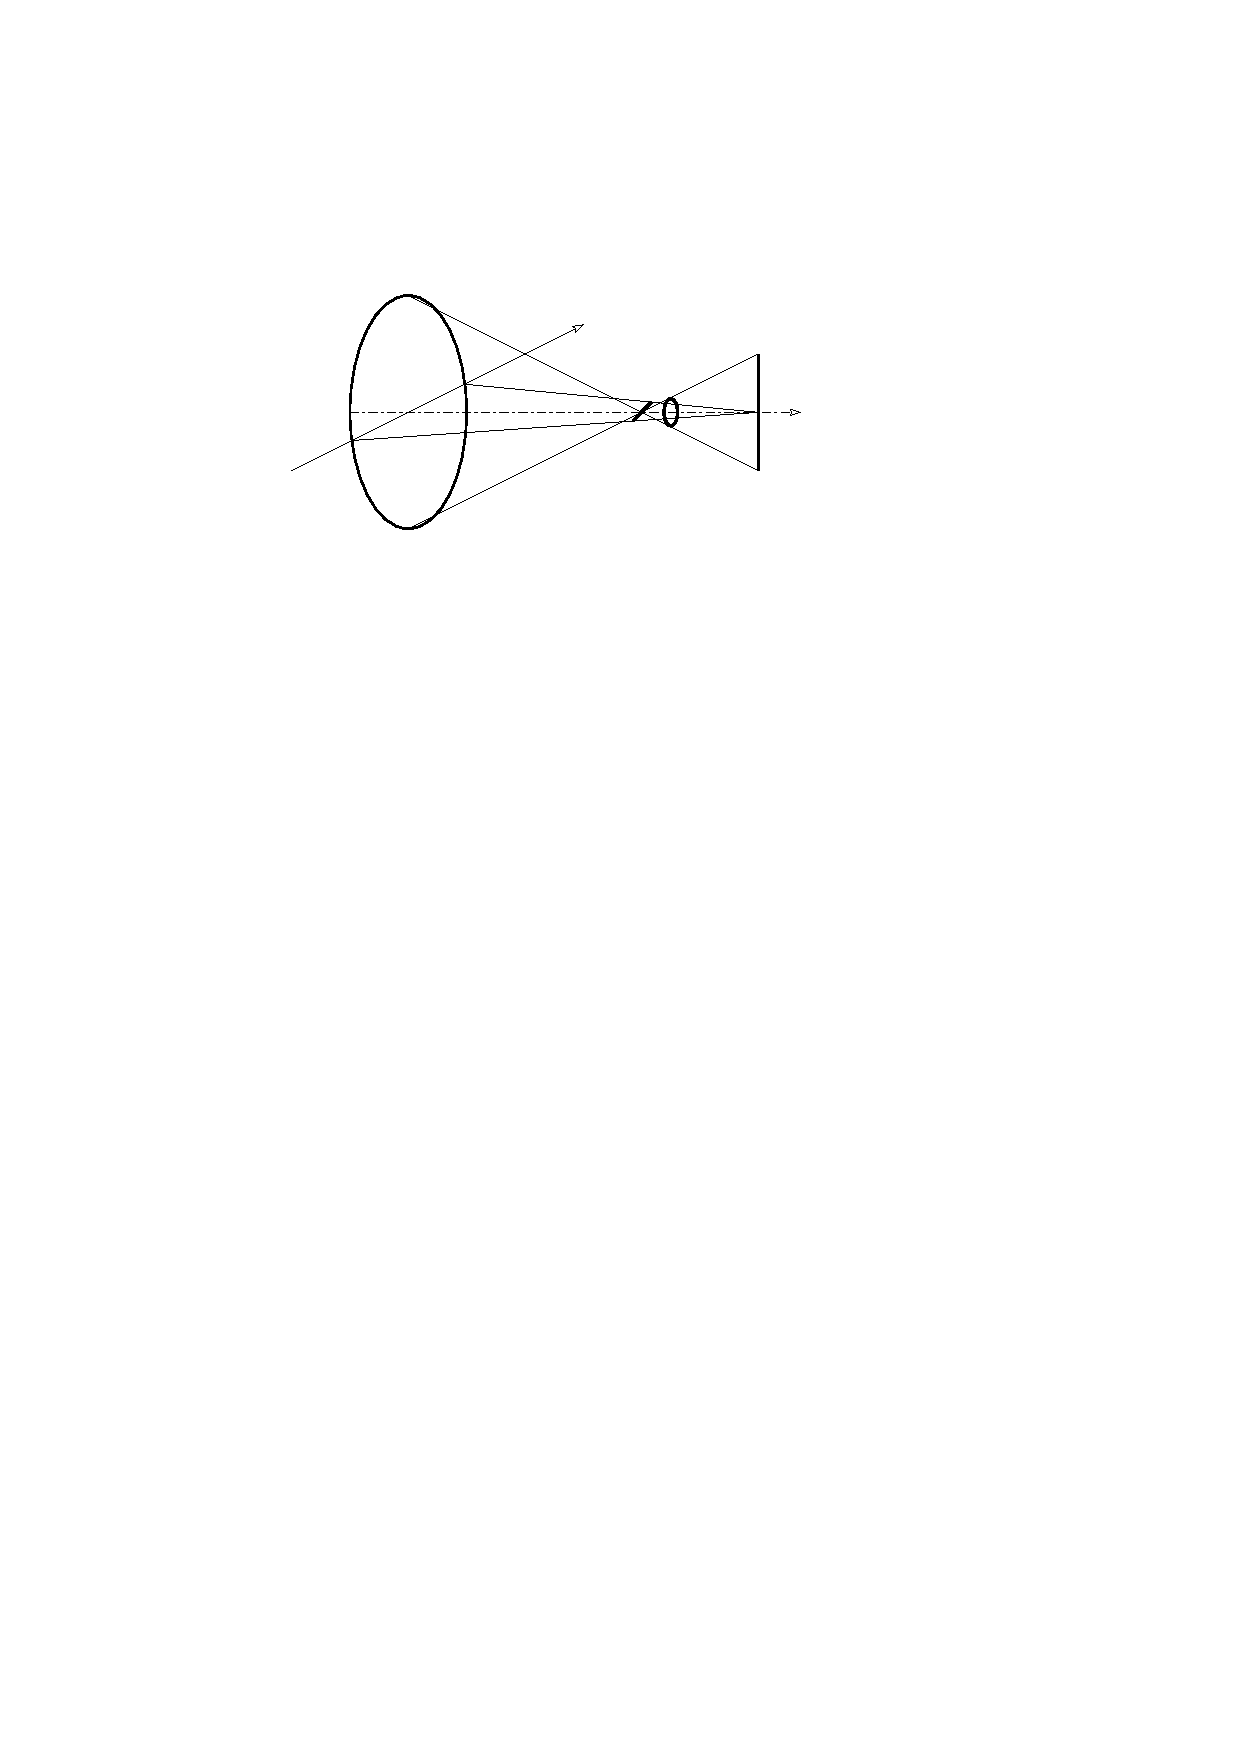
\includegraphics[width=0.4\tw]{img/astigmatism.pdf}
	\caption{}
	\label{pic:astigmatism}
\end{wrapfigure}
Астигматизм проявляется в том, что пучок лучей, исходящих из какой-либо точки, после прохождения через оптическую систему собирается не в одной точке, а на двух взаимно перпендикулярных отрезках, расположенных на некотором расстоянии друг от друга. Изображения промежуточных сечений имеют форму эллипсов.

\paragraph{Кома}

\begin{wrapfigure}[13]{l}{0.4\tw}
	\centering
	\vspace{-1pc}
	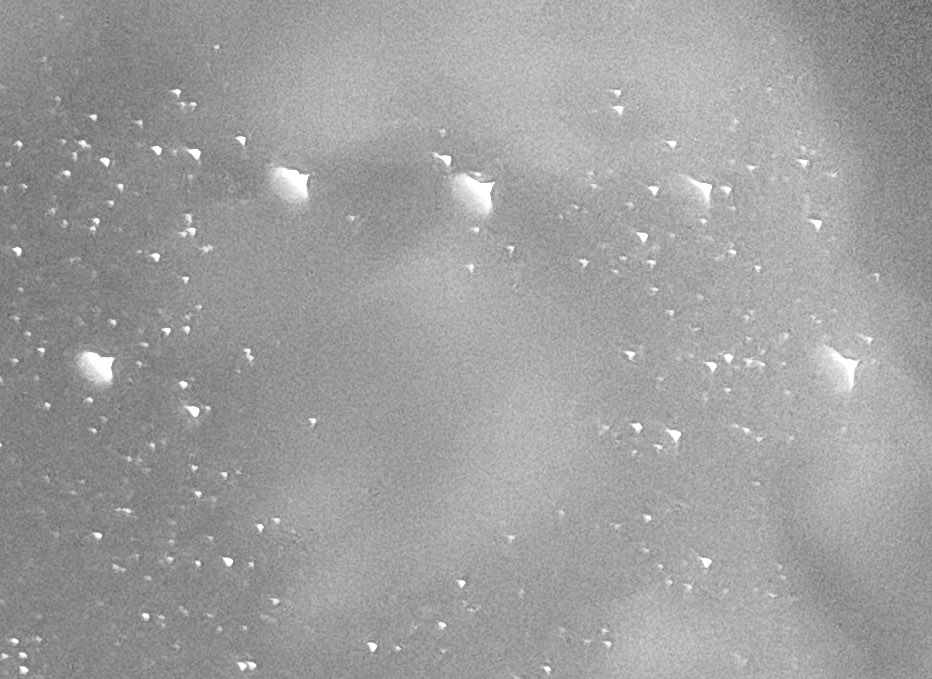
\includegraphics[width=0.4\tw]{optical-aberrations-coma.jpg}
	\caption{Изображение <<хвоста>> Большой Медведицы, полученное с помощью широкоугольного объектива, страдающего ярко выраженной комой.}
	\label{pic:optics-aberrations-coma}
\end{wrapfigure}
Один из видов аберраций оптических систем~--- аберрация широкого пучка световых лучей, проходящий наклонно к оптической оси системы, как и \imp{сферическая аберрация}, обусловлена неодинаковым преломлением световых лучей различными участками линзовых компонент системы. Кома приводит к нарушению центрированности светового пучка. В результате такой аберрации изображение точки имеет вид несимметричного пятна (см.~Рис.\,\ref{pic:optics-aberrations-coma}), по форме напоминающего запятую (англ. {\itshape comma}).

\begin{figure}[h]
	\centering
	\begin{tikzpicture}[ipe stylesheet, scale=1.1]
		%  \useasboundingbox (200, 500) rectangle (550, 750);
		\fill [lightgray] (336, 704) -- (336, 576) -- (384, 576) arc[start angle=-26.5651, end angle=26.5651, radius=143.1084] -- (336, 704);
		\draw[ipe pen fat]
		(384, 576)
		arc[start angle=-26.5651, end angle=26.5651, radius=143.1084];
		\draw[ipe pen fat]
		(336, 704)
		-- (336, 576);
		
		\draw[ipe pen heavier, ipe dash dash dotted]
		(224, 640)
		-- (500, 640);
		\draw[ipe dash dashed]
		(224, 688)
		-- (380, 688);
		\draw[ipe dash dashed]
		(304, 592)
		-- (368, 592);
		\draw[ipe dash dashed]
		(256, 640)
		-- (410.7052, 705.7731);
		\draw[ipe dash dashed]
		(256, 640)
		-- (415.3607, 594.5412);
		\draw[ipe pen heavier]
		(252, 664)
		-- (336, 688)
		-- (388, 696)
		-- (464, 650)
		-- (393, 601)
		-- (336, 592)
		-- (280, 576);
		\filldraw[fill=white]
		(435, 640) [double, line cap = butt]
		arc[start angle=180, end angle=215, radius=15];
		\node[ipe node]
		at (251.993, 630.085) {$C$};
		\draw
		(356, 700)
		-- (256, 640)
		-- (356, 580);
		\draw
		(350, 690)
		arc[start angle=9.2524, end angle=42, radius=9.7017];
		\draw
		(380, 688) [decoration={zigzag, segment length=1.1mm, amplitude=0.3mm}, decorate]
		arc[start angle=0, end angle=8.9, radius=45];
		\draw
		(316, 687.9682)
		arc[start angle=-180, end angle=-164.0101, radius=20];
		\draw
		(350, 690) [decoration={snake, segment length=1mm, amplitude=0.3mm}, decorate]
		arc[start angle=-171.1895, end angle=-157.2715, radius=38];
		\draw
		(397.3793, 690)
		arc[start angle=-20, end angle=20, radius=15];
		\draw
		(272.7114, 640.2703) [double,  line cap=butt]
		arc[start angle=0.9936, end angle=23.3266, radius=16.5778];
		\draw
		(280.6909, 632.9696)
		arc[start angle=-15.3798, end angle=0.7105, radius=25.6239];
		\node[ipe node]
		at (364.414, 642.015) {$h$};
		\node[ipe node]
		at (326.338, 662.276) {$R$};
		\node[ipe node]
		at (326.556, 621.048) {$R$};
		\draw[{ipe fptarc[ipe arrow small]}-{ipe fptarc[ipe arrow small]}]
		(240, 688)
		-- (240, 640);
		\node[ipe node]
		at (233.078, 660.549) {$d$};
		\node[ipe node]
		at (364.414, 642.015) {$h$};
		\node[ipe node]
		at (294.96, 666.059) {$l$};
		\node[ipe node]
		at (276.734, 643.661) {$\eta_1$};
		\node[ipe node]
		at (284.917, 634.094) {$\eta_2$};
		\node[ipe node]
		at (307, 683.074) {$\alpha$};
		\node[ipe node]
		at (383, 688) {\small $\beta$};
		\node[ipe node]
		at (342, 683) {\small $\gamma_1$};
		\node[ipe node]
		at (402, 693) {$\delta_1$};
		\draw
		(464, 650)
		-- (500, 620);
		\node[ipe node]
		at (425, 633) {$\omega_2$};
		\node[ipe node]
		at (457, 656) {$(x, y)$};
		\node[ipe node]
		at (408, 602) {$\delta_2$};
		\node[ipe node]
		at (366.698, 589.106) {$\beta$};
		\node[ipe node]
		at (363.462, 601.476) {$\gamma_2$};
		\node[ipe node]
		at (306.222, 586.462) {$\alpha$};
		\draw
		(316, 591.9788)
		arc[start angle=180, end angle=194.6129, radius=20];
		\draw
		(327.0296, 597.2938)
		arc[start angle=148.7026, end angle=178.4025, radius=10.533];
		\node[ipe node]
		at (314.996, 595.309) {$\xi$};
		\node[ipe node]
		at (355, 695) {\small $\xi - \beta$};
		\node[ipe node]
		at (325, 692.319) {$A_1$};
		\node[ipe node]
		at (388, 703) {$B_1$};
		\node[ipe node]
		at (324, 582) {$A_2$};
		\node[ipe node]
		at (393, 591) {$B_2$};
		\node[ipe node]
		at (338, 643) {$O$};
		\draw
		(362.1296, 591.989)
		arc[start angle=0.3563, end angle=9.2262, radius=26.1304];
		\draw
		(374.9012, 606.1184)
		arc[start angle=163.6381, end angle=187.6335, radius=19.4597];
		\draw
		(404.9644, 597.6586)
		arc[start angle=-15.516, end angle=38, radius=11.8867];
		%  \draw
		%    (580.705, 634.3486)
		%     arc[start angle=-17.9201, end angle=0.7153, radius=17.6622];
		%  \node[ipe node]
		%     at (583.258, 634.438) {$\omega_1$};
		
		%    		\foreach \x in {200, 210,...,500} {
		%				\draw [line width=.1pt] (\x, 500) -- (\x, 800);
		%				};
		%
		%				\foreach \x in {200, 300,...,500} {
		%				\draw [line width=.4pt] (\x , 500) -- (\x, 800);
		%				};
		%
		%				\foreach \y in {500, 510,...,800} {
		%				\draw [line width=.1pt] (200, \y) -- (500, \y);
		%				};
		%
		%				\foreach \y in {500, 600,...,800} {
		%				\draw [line width=.4pt] (200, \y) -- (500, \y);
		%				};
		
		\pic[ipe mark small, fill=white]
		at (256, 640) {ipe fdisk};
		\pic[ipe mark small, fill=white]
		at (336, 688) {ipe fdisk};
		\pic[ipe mark small, fill=white]
		at (388, 696) {ipe fdisk};
		\pic[ipe mark small, fill=white]
		at (336, 592) {ipe fdisk};
		\pic[ipe mark small, fill=white]
		at (464, 650) {ipe fdisk};
		\pic[ipe mark small, fill=white]
		at (393.5264, 600.6558) {ipe fdisk};
		\pic[ipe mark small, fill=white]
		at (336, 640) {ipe fdisk};
		
	\end{tikzpicture}
	\caption{}
	\label{pic:optical-aberrations-coma1}
\end{figure}

Найдем положение фокуса светового пучка, идущего под углом $\alpha$ к оптической оси. Для этого рассмотрим два луча из него, вместе с оптической осью лежащих в одной плоскости, таких, что точки преломления их передней (плоской) поверхностью линзы $A_1$ и $A_2$ лежат на расстоянии $d$ от оптической оси линзы (см.~Рис.\,\ref{pic:optical-aberrations-coma1}).

Пусть толщина линзы~--- расстояние вдоль оптической оси от вершины выпуклой поверхности, до центра плоской поверхности $O$, равно $h$. А радиус кривизны выпуклой поверхности равен $R$. Тогда расстояние $l$ от центра кривизны задней (выпуклой) поверхности линзы до точек $A_1$ и $A_2$ можно найти из теоремы Пифагора для треугольника $\triangle COA_{1,2}$:
\begin{equation*}
	l = \sqrt{(R - h)^2 - d^2}.
\end{equation*}
Равные углы $\angle A_{1,2} C O$ обозначим за $\xi$, где
\begin{equation*}
	\xi = \arcsin \frac{d}{l}.
\end{equation*}

Угол падения рассматриваемых лучей на плоскую поверхность линзы равен $\alpha$, следовательно, по закону Снеллиуса угол преломления $\beta$ определяется выражением
\begin{equation*}
	\beta = \arcsin \frac{\sin \alpha}{n},
\end{equation*}
где $n$~--- показатель преломления линзы. Обозначим углы падения верхнего и нижнего луча на заднюю поверхность линзы $\gamma_{1,2}$ соответственно. А точки преломления лучей задней поверхностью соответственно $B_{1,2}$. Запишем теорему синусов для треугольников $\triangle C A_{1,2} B_{1,2}$, чтобы найти углы $\gamma_{1,2}$ соответственно:
\begin{gather*}
	\frac{R}{\sin (180^\circ - (\xi \mp \beta))} = \frac{l}{\sin \gamma_{1,2}},\\
	\therefore \gamma_1 = \arcsin \frac{l\sin (\xi \mp \beta)}{R}.
\end{gather*}

Чтобы найти координаты точек $B_{1,2}$, определим сначала углы $ \eta_{1,2} \equiv \angle B_{1,2} C O$:
\begin{equation*}
	\eta_{1,2} = \xi - \Big[180^\circ - \gamma_{1,2} - \big(180^\circ - \left(\xi \mp \beta\right)\big)\Big] = \gamma_{1,2} \pm \beta.
\end{equation*}

Введем теперь декартову систему координат, за начало отсчета примем центр кривизны выпуклой поверхности линзы, ось $x$ направим вдоль оптической оси вправо, ось $y$ перпендикулярно вверх. В такой системе координаты точки $B_{1,2}$ задаются векторами
\begin{equation*}
	\begin{pmatrix}
		x_{1,2}\\
		y_{1,2}
	\end{pmatrix}
	= R
	\begin{pmatrix}
		\cos \eta_{1,2}\\
		\sin \eta_{1,2}
	\end{pmatrix}.
\end{equation*}
Остается воспользоваться законом Снеллиуса для определения углов $\delta_{1,2}$:
\begin{equation*}
	\delta_{1,2} = \arcsin \left( n \sin \gamma_{1,2} \right).
\end{equation*}

Поиск координат  $(x,y)$ точки пересечения лучей, вышедших из линзы начнём с поиска абсциссы. Можно заметить, что она должно удовлетворять уравнению
\begin{gather*}
	-(x - x_1) \tg \omega_1 + (x - x_2) \tg \omega_2 = y_1 + y_2,\\
	\therefore x = \frac{y_1 + y_2 - x_1\tg \omega_1 + x_2 \tg \omega_2}{\tg \omega_2 - \tg \omega_1};
\end{gather*}
где $\omega_1 = \eta_1 - \delta_1$, а $\omega_2 = -\eta_2 + \delta_2$. Теперь не сложно найти координату $y$ <<фокуса>>:
\begin{equation*}
	y = y_1 + (x - x_1) \tg \omega_1 = y_2 + (x - x_2) \tg \omega_2.
\end{equation*}

Продемонстрируем полученные зависимости (см.~Рис.\,\ref{pic:coma}), при следующих параметрах: $R = 1$, $h = 0.3$, $\alpha = 50^\circ$, $n=1.5$.

\begin{figure}[h]
	\begin{subfigure}{0.49\tw}
		\begin{tikzpicture}
			\begin{axis}[
				height	=	5cm,
				width	=	6cm,
				xlabel	=	{$d$},
				ylabel	=	{},
				ylabel shift	= 2mm,
				%			extra x ticks ={sqrt(2)/2},
				%			extra x tick labels={$\frac{\sqrt{2}}{2}$},
				xmin=0,
				xmax=0.4,
				ymin=.6,
				ymax=2,
				legend cell align=left,
				legend style={
				draw=none,
				fill=none,
				font=\scriptsize,
				at={(axis cs:.4, 2)}, anchor=north east,
%				row sep=.5pc,
				},
				]
				\addplot[smooth, gray] table[x=d, y=x] {data/coma.txt};
				\addplot[smooth] table[x=d, y=y] {data/coma.txt};
				\addplot[dashes] coordinates { (0.359606, -10) (0.359606, 1.6)};
				\legend{
				$x(d)$,
				$y(d)$,
%				$d:~\gamma_2(d)=\arcsin\frac{1}{n}$ 
				}
			\end{axis}
		\end{tikzpicture}
%		\caption{}
	\end{subfigure}
	\hfill
	\begin{subfigure}{0.49\tw}
		\begin{tikzpicture}
			\begin{axis}[
				height	=	5cm,
				width	=	6cm,
				xlabel	=	{$x$},
				ylabel	=	{$y$},
%				ylabel shift	= 2mm,
				%			extra x ticks ={sqrt(2)/2},
				%			extra x tick labels={$\frac{\sqrt{2}}{2}$},
				xmin=1.2,
				xmax=2,
				ymin=.6,
				ymax=1.1,
				]
				\addplot[only marks, mark = o, mark options={scale=0.2, black}] table[x=x, y=y] {data/coma.txt};
			\end{axis}
		\end{tikzpicture}
%		\caption{}
	\end{subfigure}
	\caption{}
	\label{pic:coma}
\end{figure}

Понятно, что смещение положение фокуса вдоль оси $x$ обусловлено \imp{сферической аберрацией}, однако смещение вдоль ось $y$ есть проявление \imp{аберрации кома}.

\paragraph{Дисторсия и кривизна фокальной поверхности}
Для тонкой линзы выполняется правило, что лучи, проходящие через оптический центр не преломляются. А световые пучки, идущие под различными углами фокусируются на фокальной плоскости, перпендикулярной оптической оси. Отсюда следует, что параллельные пучки, идущие под углом $\alpha$ к оптической оси и проходящие через оптический центр тонкой линзы, фокусируются на расстоянии $F \tg \alpha$ от оптической оси. 

\begin{figure}[h]
\begin{subfigure}{0.49\tw}
		\begin{tikzpicture}
			\begin{axis}[
				height	=	5cm,
				width	=	6cm,
				xlabel	=	{$x$},
				ylabel	=	{$y$},
%				ylabel shift	= 3mm,
				%			extra x ticks ={sqrt(2)/2},
				%			extra x tick labels={$\frac{\sqrt{2}}{2}$},
				xmin=1.25,
				xmax=3.25,
				ymin=-.2,
				ymax=1.2,
				]
				\addplot[only marks, mark = o, mark options={scale=0.2, black}] table[x=x, y=y] {data/distorsion-xy.txt};
			\end{axis}
		\end{tikzpicture}
		\caption{}
		\label{pic:pitzval}
	\end{subfigure}
	\hfill
	\begin{subfigure}{0.49\tw}
		\begin{tikzpicture}
			\begin{axis}[
				height	=	5cm,
				width	=	6cm,
				xlabel	=	{$\alpha$},
				ylabel	=	{$y(\alpha)$},
%				ylabel shift	= 1mm,
				xmin=0,
				xmax=90,
				ymin=0,
				ymax=10,
				legend cell align=left,
				legend style={
				draw=none,
				fill=none,
				font=\scriptsize,
				at={(axis cs:5, 9)}, anchor=north west,
				},
				]
				\addplot[smooth, gray] table[x=alpha, y=tan] {data/distorsion-y.txt};
				\addplot[smooth] table[x=alpha, y=y] {data/distorsion-y.txt};
				\legend{
				$2R\tg \alpha$,
				$y(\alpha)$
				}
			\end{axis}
		\end{tikzpicture}
		\caption{}
		\label{pic:distorsion-y}
	\end{subfigure}
	\caption{}
	
\end{figure}

Легко догадаться, что для толстой линзы это не выполняется. На рисунке Рис.\,\ref{pic:pitzval} показаны координаты точек фокусировки бесконечно узких пучков, падающих под углом $\alpha \in [0^\circ, 90^\circ]$ к оптической оси на центр передней поверхности рассмотренной выше плосковыпуклой линзы: ($R = 1$, $h = 0.3$, $n=1.5$, шаг составляет $1^\circ$). Отсюда ясно, что фокальная <<плоскость>> является таковой только в очень узком диапазоне направлений вокруг оптической оси. В остальной области фокальная поверхность является выпуклой в сторону от линзы.

  А на рисунке Рис.\,\ref{pic:distorsion-y} показана зависимость $y$-координаты точки фокуса от угла падения на линзу в сравнение с функцией $F \tg \alpha = 2R \tg \alpha$. Нелинейность данной зависимости от $F \tg \alpha$ проявляется в неравномерности увеличения изображения по полю зрения: чем дальше от центра, тем меньше увеличение. Такой эффект называется \term{дисторсией}, в данном случае~--- \imp{бочкообразной}, от схожести с видом деревянных бочек. Также возможна ситуация, когда $y(\alpha)$ растет быстрее $F \tg \alpha$, тогда дисторсия имеет противоположный знак и называется \imp{подушкообразной} (достаточно вспомнить, как выглядит плотно набитая подушка).
  
  \begin{figure}[h]
  \centering
\begin{subfigure}{0.31\tw}
	\centering
		\begin{tikzpicture}
			\begin{axis}[
				height	=	4cm,
				width	=	4cm,
%				xlabel	=	{$x$},
%				ylabel	=	{$y$},
%				ylabel shift	= 3mm,
				%			extra x ticks ={sqrt(2)/2},
				%			extra x tick labels={$\frac{\sqrt{2}}{2}$},
				xmin=-1.25,
				xmax=1.25,
				ymin=-1.25,
				ymax=1.25,
				hide axis
				]
				\addplot[only marks, mark = o, mark options={scale=0.2, black}] table[x=x, y=y] {data/distorsion-types.txt};
			\end{axis}
		\end{tikzpicture}
		\caption{Без дисторсии}
%		\label{pic:pitzval}
	\end{subfigure}
	\hfill
	\begin{subfigure}{0.31\tw}
	\centering
		\begin{tikzpicture}
			\begin{axis}[
				height	=	4cm,
				width	=	4cm,
%				xlabel	=	{$x$},
%				ylabel	=	{$y$},
%				ylabel shift	= 3mm,
				%			extra x ticks ={sqrt(2)/2},
				%			extra x tick labels={$\frac{\sqrt{2}}{2}$},
				xmin=-1.25,
				xmax=1.25,
				ymin=-1.25,
				ymax=1.25,
				hide axis
				]
				\addplot[only marks, mark = o, mark options={scale=0.2, black}] table[x=x_barrel, y=y_barrel] {data/distorsion-types.txt};
			\end{axis}
		\end{tikzpicture}
		\caption{Дисторсия <<бочка>>}
%		\label{pic:pitzval}
	\end{subfigure}
	\hfill
	\begin{subfigure}{0.31\tw}
	\centering
		\begin{tikzpicture}
			\begin{axis}[
				height	=	4cm,
				width	=	4cm,
%				xlabel	=	{$x$},
%				ylabel	=	{$y$},
%				ylabel shift	= 3mm,
				%			extra x ticks ={sqrt(2)/2},
				%			extra x tick labels={$\frac{\sqrt{2}}{2}$},
				xmin=-1.25,
				xmax=1.25,
				ymin=-1.25,
				ymax=1.25,
				hide axis
				]
				\addplot[only marks, mark = o, mark options={scale=0.2, black}] table[x=x_pillow, y=y_pillow] {data/distorsion-types.txt};
			\end{axis}
		\end{tikzpicture}
		\caption{Дисторсия <<подушка>>}
%		\label{pic:pitzval}
	\end{subfigure}
	\caption{Виды дисторсии}
	
\end{figure}



\subsection{Диффракция}

Электромагнитное излучение берет свое название из принципа переноса энергии, который происходит в следствие колебаний электрического и магнитного полей. В случае одномерных гармонических колебаний уравнения Максвелла имеют такое решение:
\begin{align*}
	\vec E(x, t) &= \vec E_0 \cos (k x - \omega t + \varphi_0),\\
	\vec H(x, t) &= \vec H_0 \cos (k x - \omega t + \varphi_0).
\end{align*}
\begin{wrapfigure}{l}{0.45\tw}
	\centering
	\begin{tikzpicture}[x=(-15:1.2), y=(90:1.0), z=(-150:1.0),
		line cap=round, line join=round,
		axis/.style={black, thick,->},
		vector/.style={>=stealth,->}, scale=0.5]
		\footnotesize
		\def\A{1.5}
		\def\nNodes{3} % use even number
		\def\nVectorsPerNode{8}
		\def\N{\nNodes*40}
		\def\xmax{\nNodes*pi/2*1.01}
		\pgfmathsetmacro\nVectors{(\nVectorsPerNode+1)*\nNodes}
		
		\def\vE{\mathbf{E}}
		\def\vB{\mathbf{B}}
		\def\vk{\mathbf{\hat{k}}}
		
		% main axes
		\draw[axis] (0,0,0) -- ++(\xmax*1.1,0,0) node[right] {$x$};
		\draw[axis] (0,-\A*1.4,0) -- (0,\A*1.4,0) node[right] {$y$};
		\draw[axis] (0,0,-\A*1.4) -- (0,0,\A*1.4) node[above left] {$z$};
		
		% small axes
		\def\xOffset{{(\nNodes-2)*pi/2}}
		\def\yOffset{\A*1.2}
		\def\zOffset{\A*1.2}
		\draw[axis] (\xOffset,\yOffset,-\zOffset) -- ++(\A*0.6,0,0) node[right] {$\vk$};
		\draw[axis] (\xOffset,\yOffset,-\zOffset) -- ++(0,\A*0.6,0) node[right] {$\vE$};
		\draw[axis] (\xOffset,\yOffset,-\zOffset) -- ++(0,0,\A*0.6) node[above left] {$\vB$};
		
		% waves
		\draw[very thick,variable=\t,domain=0:\nNodes*pi/2*1.01,samples=\N]
		plot (\t,{\A*sin(\t*360/pi)},0);
		\draw[very thick,variable=\t,domain=0:\nNodes*pi/2*1.01,samples=\N]
		plot (\t,0,{\A*sin(\t*360/pi)});
		
		% draw vectors
		\foreach \k [evaluate={\t=\k*pi/2/(\nVectorsPerNode+1);
		\angle=\k*90/(\nVectorsPerNode+1);
		\c=(mod(\angle,90)!=0);}]
		in {1,...,\nVectors}{
		\if\c1
		\draw[vector] (\t,0,0) -- ++(0,{\A*sin(2*\angle)},0);
		\draw[vector] (\t,0,0) -- ++(0,0,{\A*sin(2*\angle)});
		\fi
		}
	\end{tikzpicture}
	\caption{}
\end{wrapfigure}
Здесь $\vec E(x, t)$ и $\vec H (x, t)$~---  векторы напряженности электрического и магнитного полей соответственно с точке пространства с координатой $x$ в момент времени $t$. $E_0$ и $H_0$~--- амплитуды волн, которые связывает соотношение $\sqrt{\varepsilon}E_0 = \sqrt{\mu} H_0$. Остановимся на рассмотрении случая распространения излучения только в вакууме, тогда в СГС $E_0 = H_0$, так как в отсутствие среды $\varepsilon = \mu = 1$. \imp{Круговая частота} колебаний $\omega$ связана с обычной частотой колебаний $\nu$ соотношением $2\pi \nu = \omega$. А коэффициент $k$~--- \imp{волновое число}, определяемое, как $k = 2 \pi / \lambda$.

Такие волны, когда фаза волны в фиксированный момент времени зависит лишь от одной координаты, называют \imp{плоскими}. Остановимся на рассмотрении только таких волн.

Плотность потока энергии в электромагнитной волне определяется \imp{вектором Пойнтинга}:
\begin{equation}
	\vec{S} = \frac{c}{4\pi} \cross{E}{H}.
\end{equation}

Среднее значение вектора Пойнтинга называется \imp{интенсивностью излучения}:
\begin{equation}
	\vec I = \langle \vec S\rangle = \frac{c}{4\pi} \langle \cross{E}{H} \rangle.
\end{equation}
Для плоской волны в вакууме интенсивность равна
\begin{equation}
	I = \frac{c}{8\pi} E_0^2.
\end{equation}

\paragraph{Принцип Гюйгенса-Френеля}
\imp{Каждый элемент волнового фронта является центром возмущения, порождающего вторичные сферические волны, результат интерференции которых есть итоговое поле в каждой точке пространства.}

Воспользуемся данным принципом, чтобы найти поле от плоской волны после прохождения тонкой щели, то есть такой, что её ширина много меньше её длины. Пусть ширина щели равна $b$. Согласно принципу Гюйгенса-Френеля поле зависит только от угла между рассматриваемым направлением распространения излучения и осью щели. Пусть амплитуда падающей волны равна $A_0$. Тогда амплитуда от элемента ширины $dx$ в направлении $\theta$ определяется, как
\begin{equation*}
	dA = A_0 \cos (k x \sin \theta) \frac{dx}{b}.
\end{equation*}

Пусть $u \equiv k \sin \theta$, тогда суммарная амплитуда в направлении $\theta$ равна
\begin{multline*}
	A(\theta)
	= \int dA
	= \frac{A_0}{b} \int\limits_{-b/2}^{b/2} \cos ux \,d x =\\
	= \frac{A_0}{b} \left. \frac{\sin ux}{u} \right|_{-b/2}^{b/2}
	%	= \frac{A_0}{bu} \left( \sin \frac{ub}{2} - \sin \le- \frac{ub}{2} \right) = \\
	= \frac{A_0}{bu} \cdot 2 \sin \frac{bu}{2} = A_0 \left[ \sin \left( \frac{bu}{2}\right) \middle/  \frac{bu}{2} \right] .
\end{multline*}

Следовательно интенсивность определяется выражением
\begin{equation}
	I(\theta) = A^2(\theta) = A_0^2 \left[ \sin \left( \frac{bu}{2}\right) \middle/  \frac{bu}{2} \right]^2.
\end{equation}

Минимум данной функции достигается в точках, где обнуляется синус, то есть
\begin{gather*}
	\frac{bu}{2} = \pi m, \quad n \in \mathbb Z;\\
	k \sin \theta = u = \frac{2 \pi m}{b},\\
	\sin \theta = \frac{2 \pi m}{bk} = \frac{2 \pi m \lambda}{2 \pi b},\\
	\theta \simeq \sin \theta = \frac{m \lambda}{b}.
\end{gather*}
Значит первый минимум находится на $\theta = \lambda/b$.

\begin{tikzpicture}
	\begin{axis}[
		height	=	6cm,
		width	=	9cm,
		xlabel	=	{$\frac{\lambda}{b}$, $\text{м}^2$},
		ylabel	=	{$I/A_0^2$},
%		ylabel shift	= -1 cm,
		]
		
		\addplot[smooth, domain=-4:4, samples=200] {(sin(deg(x*pi))/(x*pi))^2};
	\end{axis}
\end{tikzpicture}

\begin{figure}[p]
	\centering
	\begin{subcaptionblock}{\tw}
		\begin{tikzpicture}
			\begin{axis} [
				width			=	10cm,
				colormap 		= 	{GS}{rgb(0cm)=(.1, .1, .1)  rgb(1cm)	=	(1, 1, 1)},
				xlabel 			=	{$x$, $\frac{\lambda}{D}$},
				ylabel 			=	{$y$, $\frac{\lambda}{D}$},
				zlabel 			=	{$I/I_0$},
				ylabel shift 	= -.4 cm,
				xlabel shift 	= -.3 cm,
				ytick			= {-2,0,2},
				colorbar,
				colorbar style 	= {
				ytick 	= 	{0, .2, .4, .6, .8, 1.},
				}
				]
				
				\addplot3[
				samples				=	100,
				samples y			=	100,
				mesh,
				patch type			=	line,
				x filter/.code		=	\def\pgfmathresult{-5},
				smooth
				]
				table[x=x, y=y, z=I] {data/eiry-disk-x.txt};
				%
				\addplot3[
				samples			=	100,
				samples y		=	100,
				mesh,
				patch type		=	line,
				y filter/.code	=	\def\pgfmathresult{4.5},
				smooth
				]
				table[x=x, y=y, z=I] {data/eiry-disk-y.txt};
				
				\ifthenelse{\boolean{useLightPlotVersion}}{}{
				    \addplot3[surf] table[x=x, y=y, z=I] {data/eiry-disk.txt};
				}
			\end{axis}
		\end{tikzpicture}
		\caption{}
		\label{}
	\end{subcaptionblock}\\[2pc]
	\begin{subcaptionblock}{\tw}
		\begin{tikzpicture}
			\begin{axis} [
				width			=	10cm,
				height			=	7.5cm,
				colormap 		= 	{GS}{rgb(0cm)=(.1, .1, .1)  rgb(1cm)	=	(1, 1, 1)},
				view			=	{0}{90},
				ytick 	= 	{-3, -2, ..., 3},
				colorbar,
				colorbar style 	= 	{
				ytick 	= 	{0, .2, .4, .6, .8, 1.},
				},
				xlabel 			=	{$x$, $\frac{\lambda}{D}$},
				ylabel 			=	{$y$, $\frac{\lambda}{D}$},
				]
				
				\ifthenelse{\boolean{useLightPlotVersion}}{}{
				    \addplot3[surf, shader=interp] table[x=x, y=y, z=I] {data/eiry-disk.txt};
				}
			\end{axis}
		\end{tikzpicture}
		\caption{}
		\label{}
	\end{subcaptionblock}
	\caption{}
\end{figure}

\begin{figure}[p]
	\centering
	\begin{subcaptionblock}{\tw}
		\begin{tikzpicture}
			\begin{axis} [
				width			=	10cm,
				colormap 		= 	{GSW}{rgb(0cm)=(.1, .1, .1) rgb(.05cm)=(.99, .99, .99) rgb(1cm)	=	(1, 1, 1)},
				xlabel 			=	{$x$, $\frac{\lambda}{D}$},
				ylabel 			=	{$y$, $\frac{\lambda}{D}$},
				zlabel 			=	{$I/I_0$},
				ylabel shift 	= -.4 cm,
				xlabel shift 	= -.3 cm,
				ytick			= {-2,0,2},
				colorbar,
				colorbar style 	= {
				ytick 	= 	{0, .2, .4, .6, .8, 1.},
				}
				]
				
				\addplot3[
				samples				=	100,
				samples y			=	100,
				mesh,
				patch type			=	line,
				x filter/.code		=	\def\pgfmathresult{-5},
				smooth
				]
				table[x=x, y=y, z=I] {data/eiry-disk-x.txt};
				%
				\addplot3[
				samples			=	100,
				samples y		=	100,
				mesh,
				patch type		=	line,
				y filter/.code	=	\def\pgfmathresult{4.5},
				smooth
				]
				table[x=x, y=y, z=I] {data/eiry-disk-y.txt};
				
				\ifthenelse{\boolean{useLightPlotVersion}}{}{
				    \addplot3[surf] table[x=x, y=y, z=I] {data/eiry-disk.txt};
				}
			\end{axis}
		\end{tikzpicture}
		\caption{}
		\label{}
	\end{subcaptionblock}\\[2pc]
	\begin{subcaptionblock}{\tw}
		\begin{tikzpicture}
			\begin{axis} [
				width			=	10cm,
				height			=	7.5cm,
				colormap 		= 	{GSW}{rgb(0cm)=(.1, .1, .1) rgb(.05cm)=(.99, .99, .99) rgb(1cm)	=	(1, 1, 1)},
				view			=	{0}{90},
				ytick 	= 	{-3, -2, ..., 3},
				colorbar,
				colorbar style 	= 	{
				ytick 	= 	{0, .2, .4, .6, .8, 1.},
				},
				xlabel 			=	{$x$, $\frac{\lambda}{D}$},
				ylabel 			=	{$y$, $\frac{\lambda}{D}$},
				]
				
				\ifthenelse{\boolean{useLightPlotVersion}}{}{
				    \addplot3[surf, shader=interp] table[x=x, y=y, z=I] {data/eiry-disk.txt};
				}
			\end{axis}
		\end{tikzpicture}
		\caption{}
		\label{}
	\end{subcaptionblock}
	\caption{}
\end{figure}

\begin{figure}[p]
	\begin{subcaptionblock}[t]{\tw}
		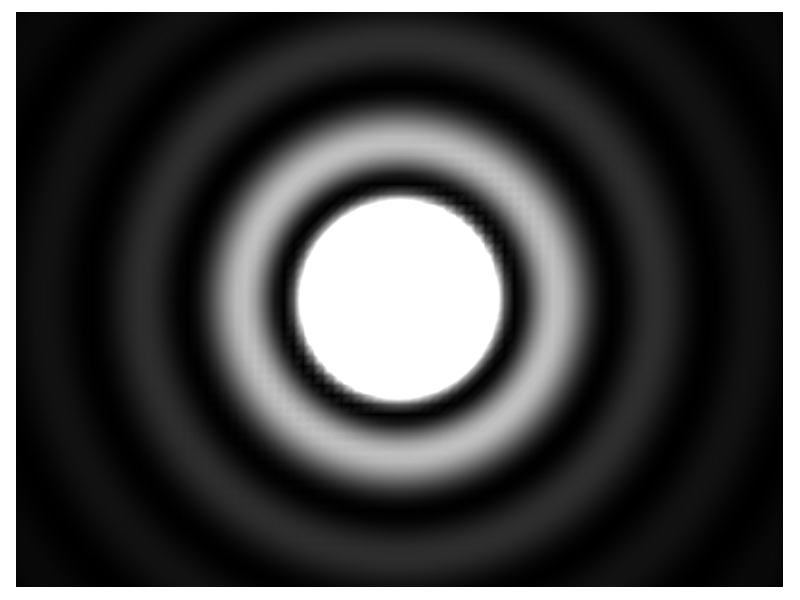
\includegraphics[width=4.7cm]{eiry-disk-0}\hfill
		\begin{tikzpicture}
			\begin{axis}[
				height	=	4.125cm,
				width	=	5.5cm,
				xlabel	=	{$x$, $\frac{\lambda}{D}$},
				ylabel	=	{$I/I_0$},
%				ylabel shift	= -1.1 cm,
				]
				
				\addplot[smooth] table[x=x, y=e0]{data/eiry-disk-profile.txt};
			\end{axis}
		\end{tikzpicture}
		\caption{Диффракционное изображение от одного источника}
	\end{subcaptionblock}\\
	\begin{subcaptionblock}[t]{\tw}
		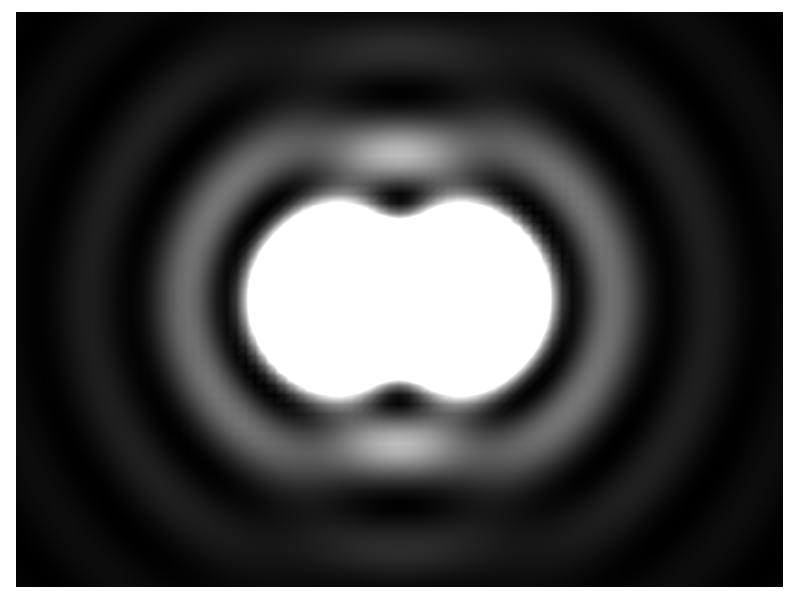
\includegraphics[width=4.7cm]{eiry-disk-1}\hfill
		\begin{tikzpicture}
			\begin{axis}[
				height	=	4.125cm,
				width	=	5.5cm,
				xlabel	=	{$x$, $\frac{\lambda}{D}$},
				ylabel	=	{$I/I_0$},
%				ylabel shift	= -1.1 cm,
				]
				
				\addplot[smooth] table[x=x, y=e1]{data/eiry-disk-profile.txt};
			\end{axis}
		\end{tikzpicture}
		\caption{Диффракционное изображение от двух источников с разделением~$1.22\lambda/D$}
	\end{subcaptionblock}\\
	\begin{subcaptionblock}{\tw}
		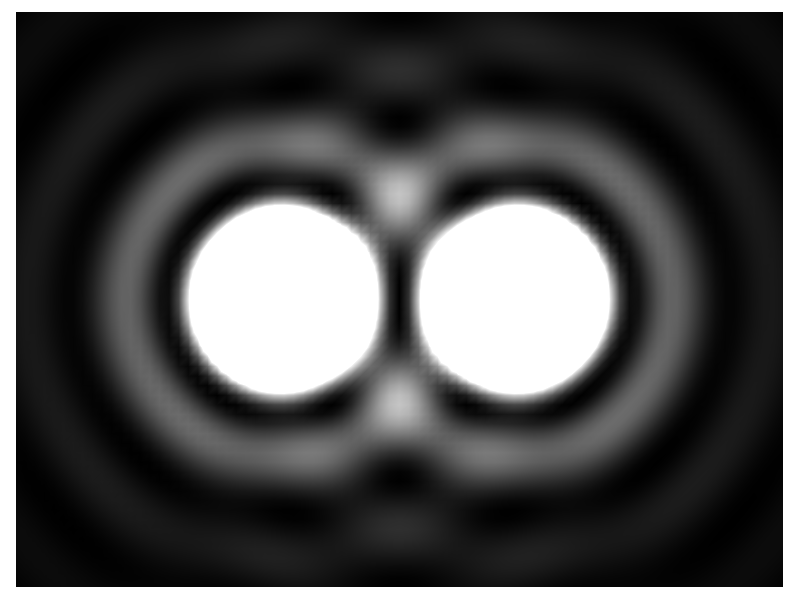
\includegraphics[width=4.7cm]{eiry-disk-2}\hfill
		\begin{tikzpicture}
			\begin{axis}[
				height	=	4.125cm,
				width	=	5.5cm,
				xlabel	=	{$x$, $\frac{\lambda}{D}$},
				ylabel	=	{$I/I_0$},
%				ylabel shift	= -1.1 cm,
				]
				
				\addplot[smooth] table[x=x, y=e2]{data/eiry-disk-profile.txt};
			\end{axis}
		\end{tikzpicture}
		\caption{Диффракционное изображение от двух источников с разделением~$2 \cdot 1.22\lambda/D$}
	\end{subcaptionblock}\\
	\begin{subcaptionblock}{\tw}
		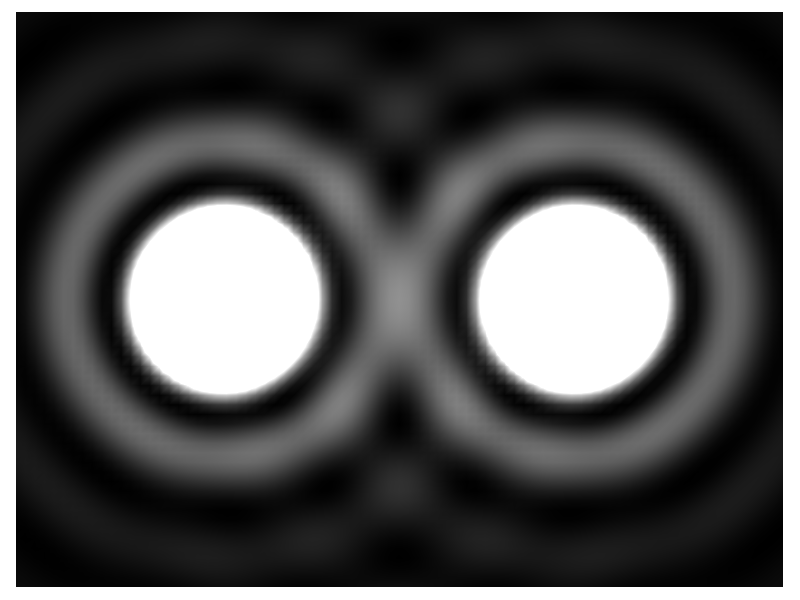
\includegraphics[width=4.7cm]{eiry-disk-3}\hfill
		\begin{tikzpicture}
			\begin{axis}[
				height	=	4.125cm,
				width	=	5.5cm,
				xlabel	=	{$x$, $\frac{\lambda}{D}$},
				ylabel	=	{$I/I_0$},
%				ylabel shift	= -1.1 cm,
				]
				
				\addplot[smooth] table[x=x, y=e3]{data/eiry-disk-profile.txt};
			\end{axis}
		\end{tikzpicture}
		\caption{Диффракционное изображение от двух источников с разделением~$3 \cdot 1.22\lambda/D$}
	\end{subcaptionblock}
	\caption{}
\end{figure}




	\section{Сферическая астрономия}

Раздел сферической астрономии или небесной сферы собирает в себе темы, связанные с положением и движением небесных тел по небесной сфере в результате суточного и годичного движение Земли. Для дальнейшего повествования определим некоторые термины, на которых оно будет построено.

\term{Большой круг сферы}~--- окружность на поверхности сферы, центр которого совпадает с центром сферы.

Здесь и далее \imp{осью вращения} будем называть неподвижную ось вращения сферы, проходящую через ее центр. 

\term{Экватор}~--- большой круг, перпендикулярный оси вращения. Точки пересечения оси вращения со сферой называются \term{полюсами}.

\term{Малый круг сферы}~--- произвольная окружность на поверхности сферы. \term{Параллель}~--- малый круг, параллельный экватору.

Большой круг, перпендикулярный экватору, называется \term{мери\-диа\-ном}. Угловое расстояние между заданной точкой $A$ и точкой пересечения меридиана, проходящего через точку $A$, с экватором называется \term{широтой} точки $A$. Широта обозначается греческой буквой $\varphi$. В северном полушарии $\varphi > 0$, в южном~--- $\varphi < 0$. Очевидно, $\varphi \in [-90; 90]$. \term{Полярное расстояние}~$p$~--- угловое расстояние между рассматриваемой точкой и точкой северного полюса. $p + \varphi = 90^\circ$.

Теперь можно перейти от геометрии к астрономии. 

\term{Наблюдатель}~--- материальная точка на поверхности сферы (Земли). \term{Небесная сфера}~--- воображаемая сфера произвольного (бесконечного) радиуса с центром в наблюдателе. \term{Точка небесной сферы}~--- воображаемая точка на небесной сфере, на самом деле являющаяся некоторым лучом с заданным направлением.

\term{Математический горизонт}~--- касательная плоскость к поверхности сферы в наблюдателе. Чаще математическим горизонтом называют большой круг небесной сферы~--- пересечение вышеописанной плоскости с небесной сферы. 

\term{Зенит}~$Z$~--- (точка небесной сферы) луч, исходящий из наблюдателя от, перпендикулярный математическому горизонту, направлен от центра сферы. эквивалентично определяется точка \term{надира}~$Z'$, противоположная точке зенита.

\term{Полярная ось}~--- ось вращения небесной сферы, параллельная оси вращения Земли. \term{Полюс мира} (северный)~$P$~--- точка пересечения полярной оси с небесной сферой со стороны северного полюса Земли. Южный \imp{полюс мира}~$P'$~--- точка, противоположная северному полюсу мира.

Здесь возникает проблема: Земля вращается, а значит наблюдатель движется, и небесная небесная сфера смещается. То есть положения на небесной сфере неподвижных в пространстве звезд меняются. Это называется параллаксом, а котором говорилось в Разделе ??. 

В силу малости горизонтального параллакса можно сделать вывод, что для далеких небесных объектов можно им пренебречь и считать их неподвижными. Также в большинстве задач сферической астрономии пренебрегают и годичным параллаксом, хотя его величина уже не исчезающе мала. 

Однако из этого всего не следует, что нужно совсем забывать про явления параллакса. Важно при решении каждой задачи на сферическую астрономию проверять необходимость учета этого явления.

Так или иначе, пренебрегая размером Земли, можно считать, что наблюдатель находится в центре Земли. А плоскостью математического горизонта, все также проходит через наблюдателя и параллельна изначальной.

\term{Небесный экватор}~--- большой круг небесной сферы, перпендикулярный полярной оси. \term{Суточная параллель}~--- путь неподвижного небесного объекта в течение суток по небесной сфере, является малым кругом, эквивалент~--- параллель.

\term{Север}~$N$ и \term{юг}~$S$~--- точки небесной сферы на математическом горизонте, лежащие на одном луче с проекциями соответствующих полюсов мира на математический горизонт.

Нетрудно показать, что точки $P$~--- северный полюс мира, $P'$~--- южный полюс мира, $Z$~--- зенит, $Z'$~--- надир, $N$~--- север и $S$~---юг лежат на одном большом круге. Этот круг называется \term{небесным меридианом}.


\subsection{Системы небесных координат}
Каждая из систем небесных координат является сферической системой координат, в которой радиус не имеет значения, так как параллакс не учитывается, а объекты считаются бесконечно удалёнными от наблюдателя.

\begin{figure}[!h]
	\centering
	\begin{subcaptionblock}{0.49\textwidth}
		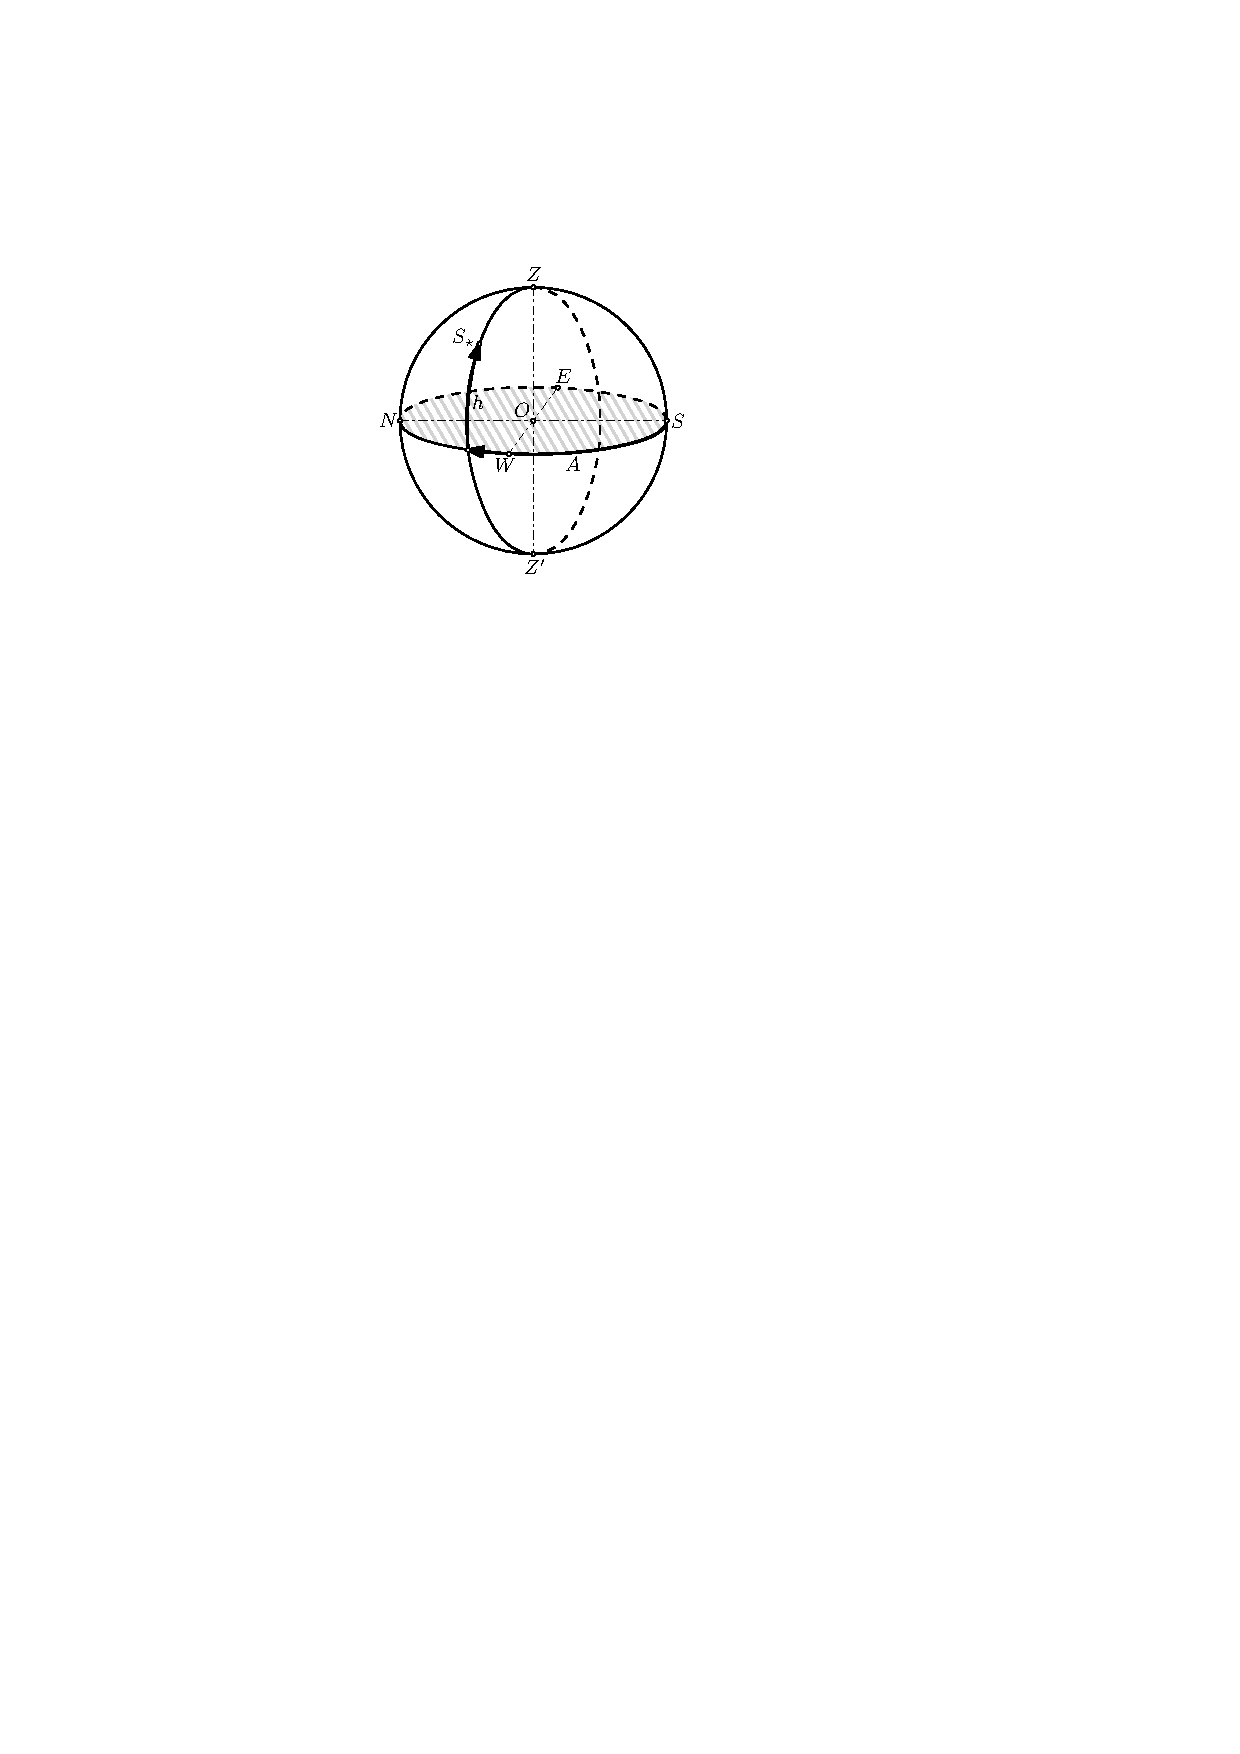
\includegraphics[width = \textwidth]{hor-coordin-sys}
		\caption{Горизонтальная система координат}
	\end{subcaptionblock}
	\hfill
	\begin{subcaptionblock}{0.49\textwidth}
		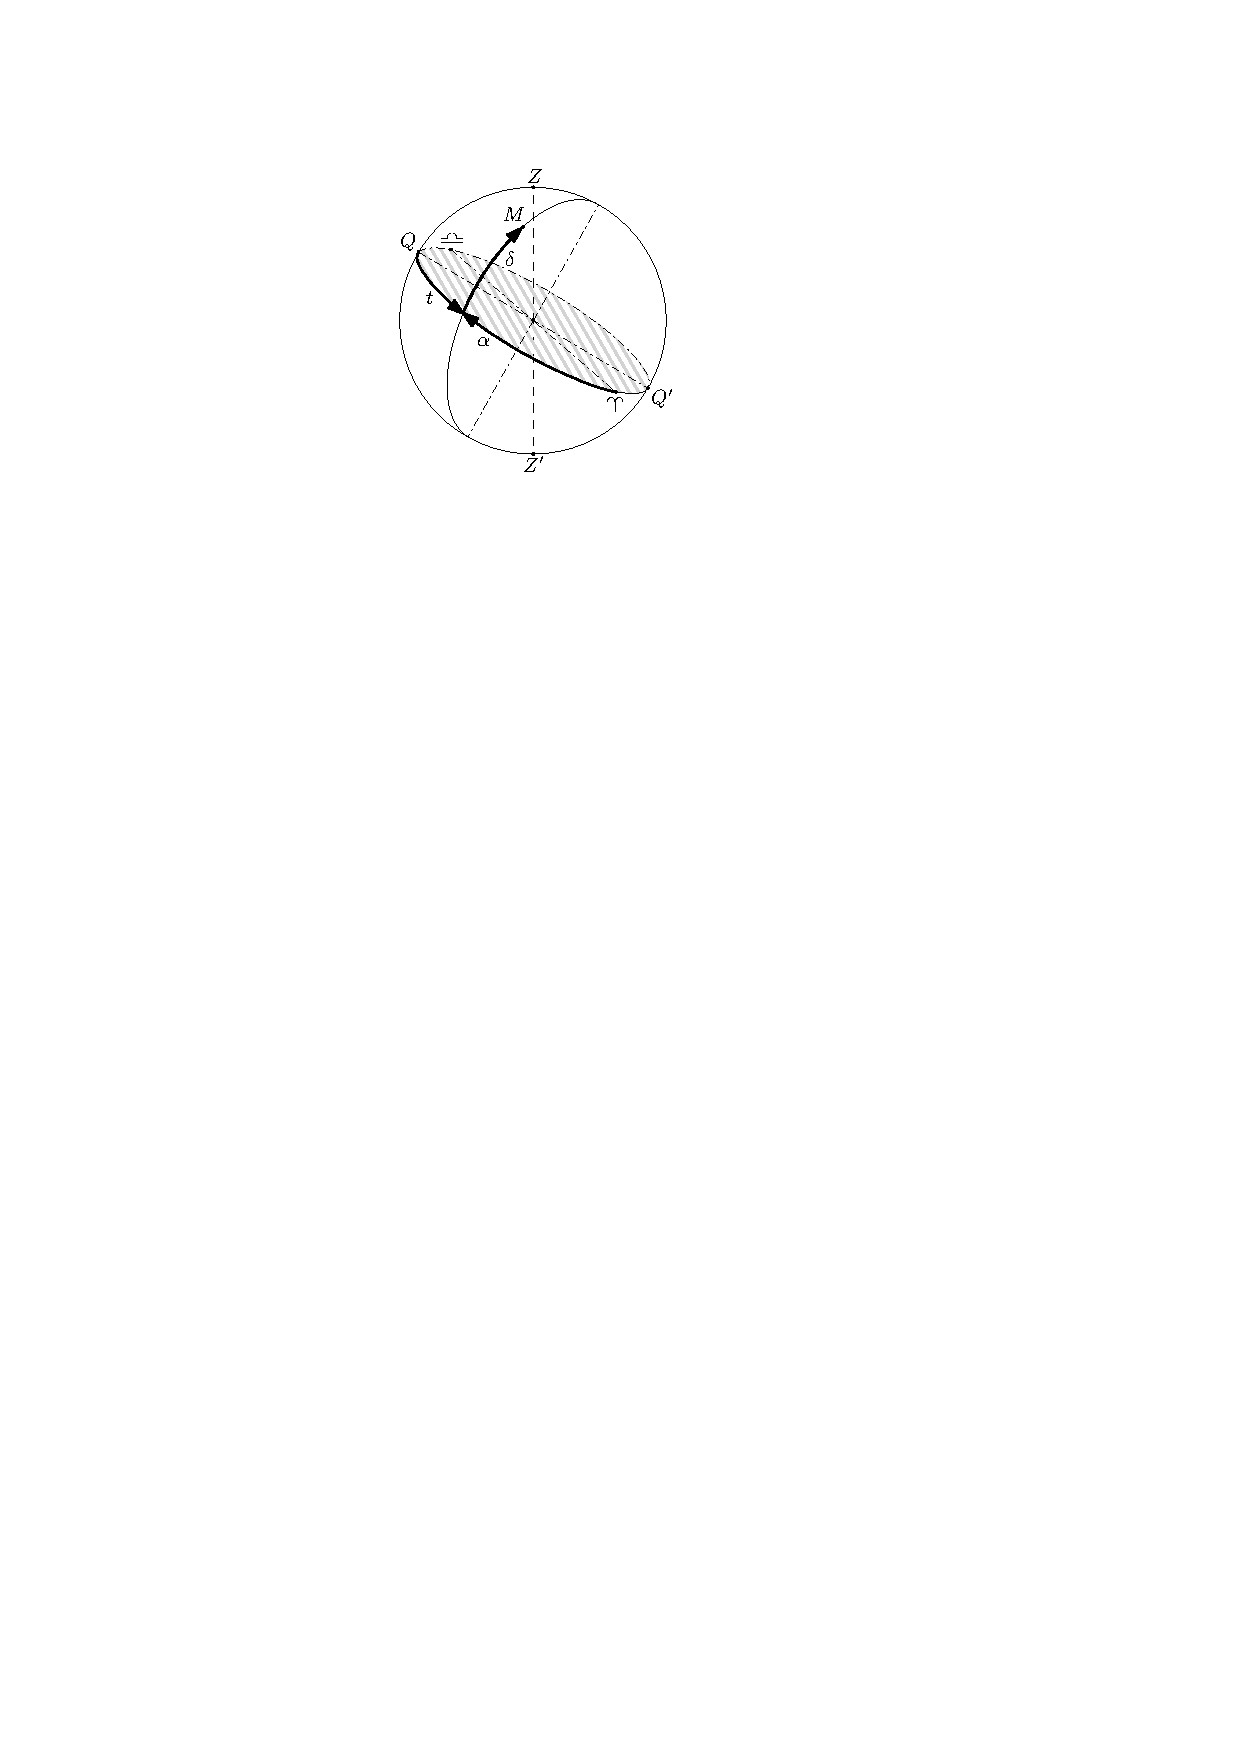
\includegraphics[width = \textwidth]{eq-coordin-sys}
		\caption{Экваториальная система координат}
	\end{subcaptionblock}
	\caption{Системы координат I}
\end{figure}
\term{Горизонтальная система координат}~--- система координат, в которой основной плоскостью является плоскость математического горизонта, а полюсами~--- \term{зенит} и \term{надир}~--- точки небесной сферы, расположенные ровно над наблюдателем и под ним соответственно. Одной координатой является либо \term{высота} светила $h$~--- угловое расстояние между светилом и математическим горизонтом, отсчитываемое в сторону зенита, либо его \term{зенитное расстояние}~$z$~--- угловое расстояние между зенитом и светилом. Другой координатой является \term{астрономический азимут} $A$~--- угол $SZS_\star$, отсчитываемый в сторону запада. Половина большого круга, перпендикулярного горизонту,~--- $Z S_\star Z'$  называется \term{вертикалом} объекта.

\term[экваториальная система координат]{Первая экваториальная система координат}~--- система координат,
основной плоскостью которой является плоскость небесного экватора $QEQW'$.
Одной координатой при этом является \term{склонение}~$\delta$~--- угловое
расстояние между светилом и плоскостью небесного экватора, отсчитываемое в
сторону севера. Половина большого круга, вдоль которой отсчитывается склонение,
перпендикулярна небесному экватору и называется \term[круг склонений]{кругом склонений} или
\imp{кругом равных часовых углов (прямых восхождений)}. Наряду со склонением
используется \term{полярное расстояние}~$p$~--- угловое расстояние между
светилом и полюсом мира. Другой координатой является \term{часовой угол}~$t$~---
дуга небесного экватора от верхней точки небесного экватора до круга склонения
светила в сторону запада, или угол между небесным меридианом и кругом склонения
светила. $\aries$ и $\libra$~--- точки весеннего и осеннего равноденствия соответственно.

\term[экваториальная система координат]{Вторая экваториальная система координат}~--- система, аналогичная предыдущей. Одной координатой по прежнему является \term{склонение}~$\delta$. А другой координатой является \term{прямое восхождение}~$\alpha$~--- угловое расстояние между точкой весеннего равноденствия и кругом склонений светила в сторону годичного движения Солнца.

\begin{figure}[!h]
	\centering
	\begin{subcaptionblock}{0.49\textwidth}
		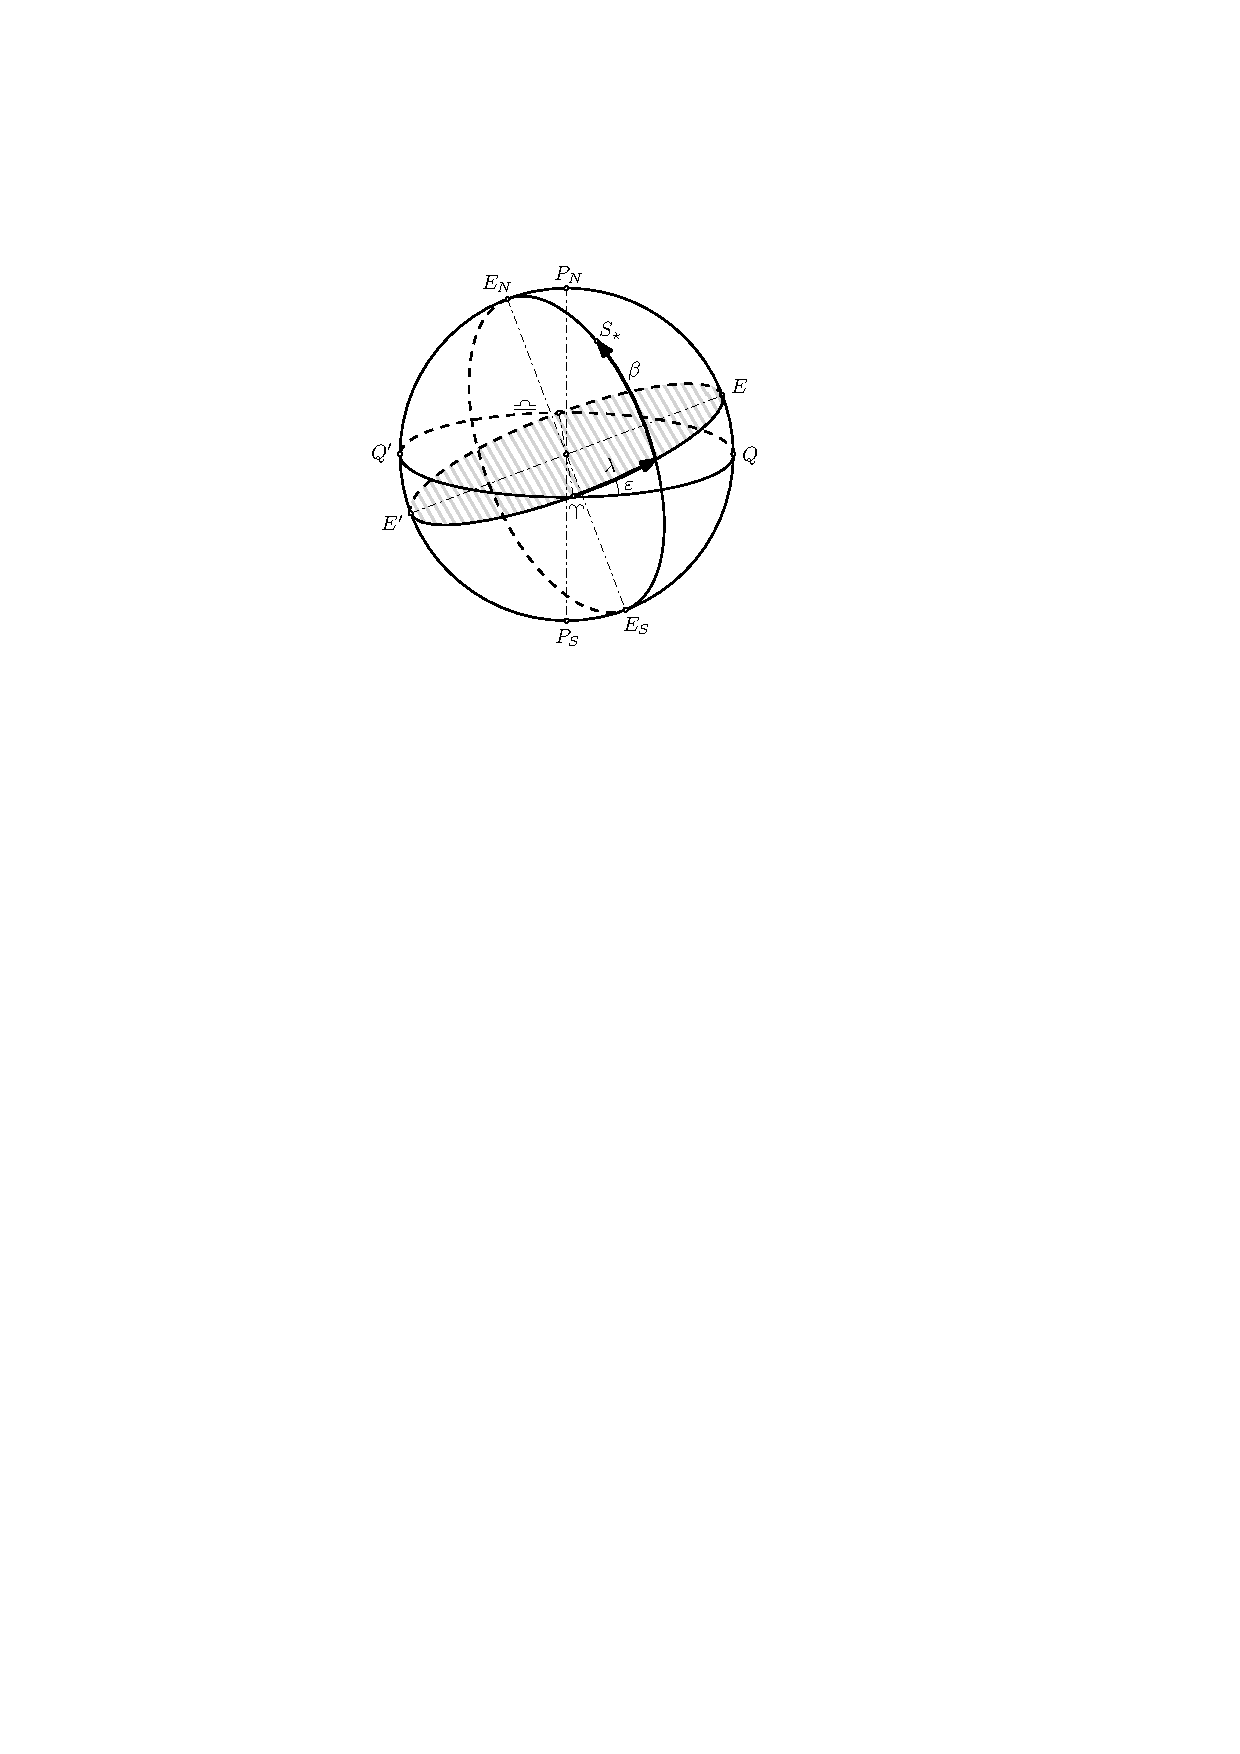
\includegraphics[width = \textwidth]{eql-coordin-sys}
		\caption{Эклиптическая система координат}
	\end{subcaptionblock}
	\hfill
	\begin{subcaptionblock}{0.49\textwidth}
		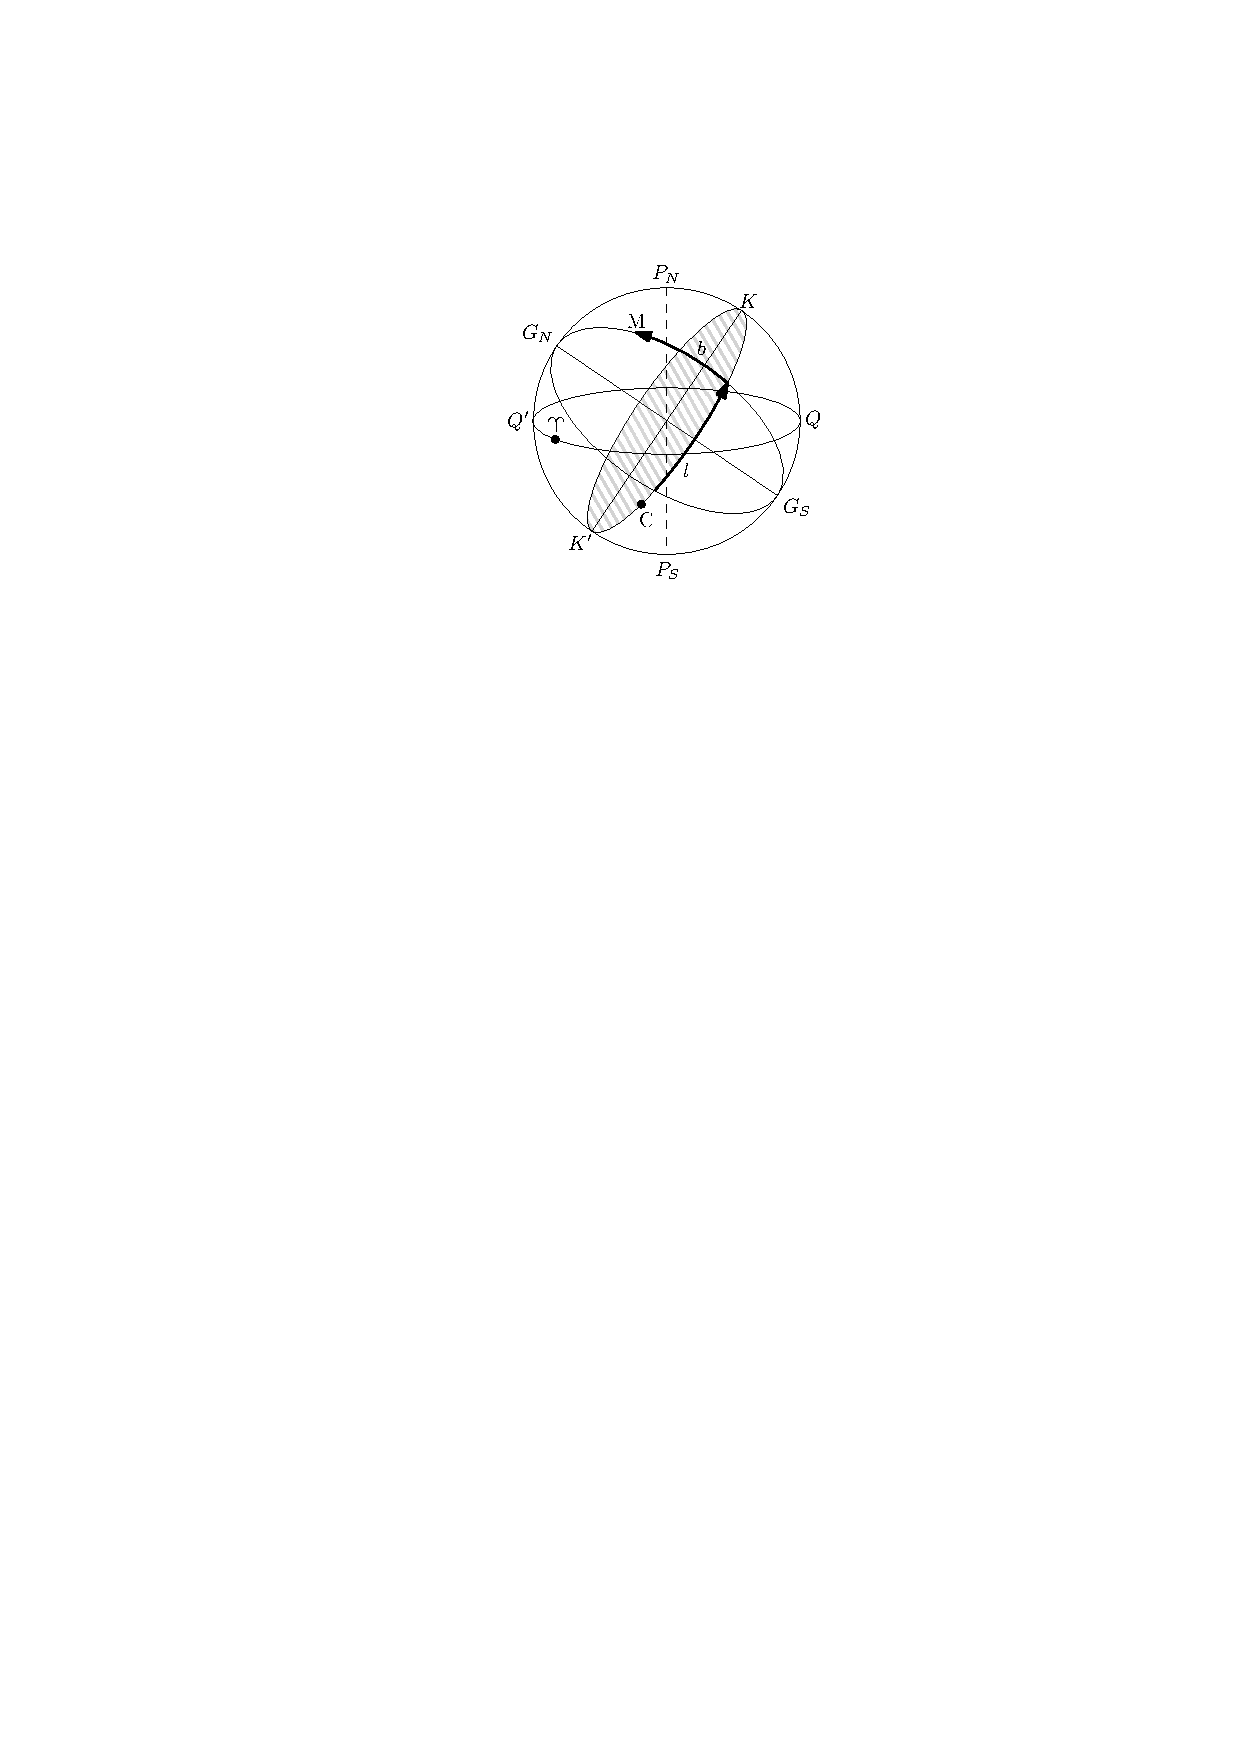
\includegraphics[width = \textwidth]{gal-coordin-sys}
		\caption{Галактическая система координат}
	\end{subcaptionblock}
	\caption{Системы координат II}
\end{figure}
\term{Эклиптическая система координат}~--- система координат, основной плоскостью которой является плоскость эклиптики $E \libra E' \aries $. Одной координатой при этом является \term{эклиптическая широта}~$\beta$~--- угловое расстояние между светилом и плоскостью эклиптики, отсчитываемое в сторону северного полюса мира, а другой~--- \term{эклиптическая долгота}~$\lambda$~--- угловое расстояние между точкой весеннего равноденствия и кругом эклиптической широты светила. Полюса эклиптики $E_N$ и $E_S$ имеют координаты ($18^h$,~$90^\circ - \varepsilon$) и ($6^h$,~$-90^\circ + \varepsilon$).

\term{Галактическая система координат}~--- система координат, основной плоскостью которой является плоскость нашей галактики, которая наклонена к плоскости небесного экватора под углом $62.6^\circ$. Одной координатой при этом является \term{галактическая широта}~$b$~--- угол между плоскостью галактического экватора и направлением на светило, а другой~--- \term{галактическая долгота}~$l$~--- угол между направлением на точку начала отсчёта $C$ и плоскостью круга галактической широты светила. Точка $C$ является направлением на центр галактики и имеет координаты: $\alpha=17^h\,45.6^m$, $\delta=-28^{\circ}\,56.2'$. $C K K'$~--- плоскость галактического экватора; $G_N$, $G_S$~--- северный и южный полюса галактики соответственно.

\subsection{Суточное вращение небесной сферы}
Вследствие вращения Земли вокруг своей оси для наблюдателя на поверхности небесные объекты совершают суточное движение параллельно небесному экватору, плоскость которого совпадает с плоскостью экватора Земли. Очевидно, в ходе такого движения высота светил постоянно меняется и в некоторые моменты времени достигает своего максимального и минимального значения.

\term[верхняя кульминация]{Верхняя} и \term{нижняя кульминация}~--- моменты пересечения светилом небесного меридиана, причём при верхней кульминации светило имеет наибольшую высоту, а при нижней~--- наименьшую.

Высота светила в верхней и нижней кульминации со склонением $|\delta| < |\varphi|$, соответственно:
\begin{equation}
	h_{\text{в}}= 90^\circ - \varphi + \delta, \quad\quad
	h_{\text{н}}= - 90^\circ + \varphi  + \delta.
\end{equation}

Если же светило имеет склонение $|\delta| > |\varphi|$, то высота в верхней и нижней кульминации вычисляется так:
\begin{equation}
	h_{\text{в}}= 90^\circ + \varphi - \delta, \quad\quad
	h_{\text{н}}= - 90^\circ -\varphi - \delta.
\end{equation}

Из формул для высоты в нижней кульминации вытекает условие, определяющее, пересекает ли звезда горизонт:
\begin{equation}
	\begin{cases}
		h_\text{в} = +90^\circ - |\varphi - \delta| > 0^\circ,\\
		h_\text{н} = - 90^\circ + |\varphi + \delta| < 0^\circ;
	\end{cases}
	\quad \Longleftrightarrow \quad~~ |\delta|< 90^{\circ} - |\varphi|.
\end{equation}

Используя формулы сферической тригонометрии (см.\,\ref{sec:spher-trig}), можно выразить зависимость часового угла светила от его зенитного расстояния:
\begin{equation}
	\cos t=\frac{\cos z-\sin\varphi\sin\delta}{\cos\varphi\cos\delta}.
\end{equation}
Отсюда следует, что для часового угла захода и восхода светила справедливо равенство:
\begin{equation}
	\cos t_{\uparrow\downarrow}=-\tg\varphi\cdot\tg\delta.
\end{equation}

Аналогично, для вычисления азимута светила верна формула
\begin{equation}
	\cos A=\frac{\cos\delta\cos t-\cos\varphi\cos z}{\sin\varphi\sin z}.
\end{equation}
Следовательно, азимуты точек восхода и захода
\begin{equation}
	A_\uparrow = \arccos \left(-\dfrac{\sin\delta}{\cos \varphi} \right)\quad\text{и}\quad A_\downarrow = - A_\uparrow.
\end{equation}

\term{Звёздное время}~$z$~--- часовой угол точки весеннего равноденствия. Из определений прямого восхождения и часового угла следует справедливость равенства\begin{equation}
z = \alpha + t.
\end{equation}

\subsection{Сферическая тригонометрия}
\label{sec:spher-trig}
\begin{wrapfigure}[10]{r}{.3\tw}
    \centering
    \vspace{-1pc}
    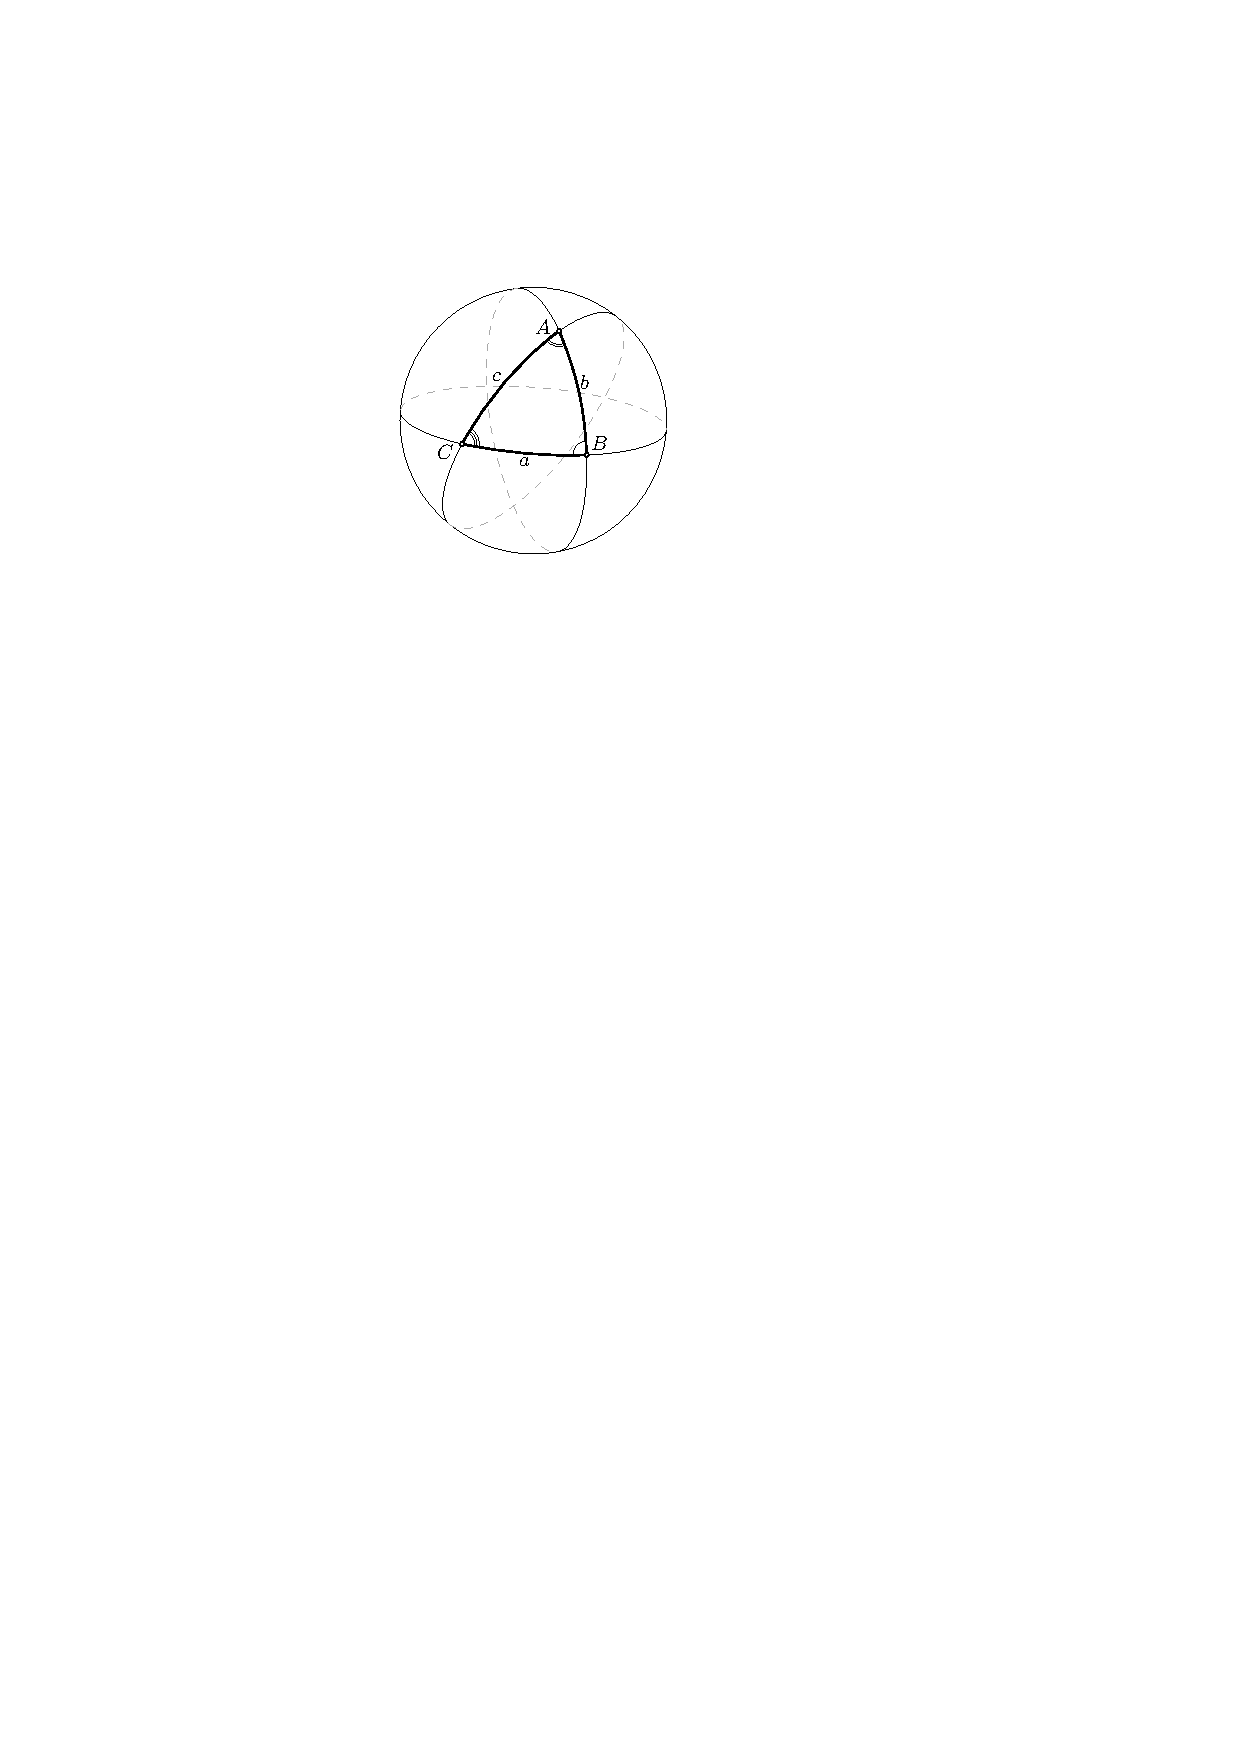
\includegraphics[width=0.3\textwidth]{spher-trigonom}
    \caption{Сферический треугольник}
\end{wrapfigure}
Для решения некоторых задач астрономии, связанных с видимыми положениями небесных тел, требуются знания о сферической тригонометрии. \imp{Сферический треугольник}~--- фигура на поверхности сферы, состоящая из трёх точек и трёх дуг больших кругов, соединяющих эти точки. Пусть $A$, $B$ и $C$~--- углы сферического треугольника, а $a$, $b$ и $c$~--- его стороны.

Сферические треугольники обладают следующими свойствами:
\begin{enumerate}
    \item Два сферических треугольника равны, если они подобны.
    \item Каждая сторона меньше суммы двух других сторон и больше их разности.
    \item Сумма всех сторон $a+b+c$ всегда меньше $2\pi$.
    \item Сумма углов сферического треугольника $\pi < A + B + C < 3\pi$.
    \item Разность суммы двух углов и третьего угла меньше $\pi$
\end{enumerate}

Площадь сферического треугольника определяется по формуле:
\begin{equation}
    S = R^2( A + B + C - \pi),
\end{equation}
где $A + B + C - \pi$~--- \imp{сферический избыток}.

Рассмотрим сферический треугольник $ABC$, радиус векторы вершин соответственно $\vec{a}$, $\vec{b}$ и $\vec{c}$.Причем из определения сферы $|\vec{a}| = |\vec{b}| = |\vec{c}| = r$. Пусть против вершин $A$, $B$ и $C$ лежат стороны с угловой мерой $a$, $b$ и $c$ соответсвенно. Повернем сферические координаты и нормируем так, чтобы $\vec{a} = (0, 0, 1)$, $\vec{b} = (\sin c, 0, \cos c)$, тогда $ \vec{c} = (\sin b \cos A, \sin b \sin A, \cos b)$.

Теперь запишем выражение для $\scalar{b}{c}$:
\begin{equation}
    \scalar{b}{c} = \cos a = \sin c \sin b \cos A + \cos c \cos b.
    \label{eq:spher-astro-cos-1}
\end{equation}
Аналогично,
\begin{gather}
    \scalar{a}{c} = \cos b = \sin a \sin c \cos B +  \cos a \cos c,\\
    \scalar{a}{b} = \cos c = \sin a \sin b \cos C + \cos a \cos b.
    \label{eq:spher-astro-cos-1-1}
\end{gather}
Выразим отсюда $\cos A$:
\begin{equation}
    \cos A = \frac{\cos a - \cos c \cos b}{\sin c \sin b}.
    \label{eq:spher-astro-cos-2}
\end{equation}
Формулы \eqref{eq:spher-astro-cos-1}\,--\,\eqref{eq:spher-astro-cos-2} называются \term{сферической теоремой косинусов} \imp{для стороны} \eqref{eq:spher-astro-cos-1}\,--\,\eqref{eq:spher-astro-cos-1-1} и, соответственно \imp{для угла} \eqref{eq:spher-astro-cos-2}.

Из основного тригонометрического тождества имеем:
\begin{multline*}
    \sin^2 A = 1 - \cos^2 A = 1 - \left[ \frac{\cos a - \cos c \cos b}{\sin c \sin b} \right]^2 = \\
    = \frac{\sin^2 c \sin^2 b - \cos^2 a + 2\cos a \cos c \cos b - \cos^2 c \cos^2 b}{\sin^2 c \sin^2 b}=\\
    = \frac{(1 - \cos^2 c)(1 -  \cos^2 b) - \cos^2 a + 2\cos a \cos c \cos b - \cos^2 c \cos^2 b}{\sin^2 c \sin^2 b}=\\
    = \frac{1 - \cos^2 c - \cos^2 b + \cos^2 c \cos^2 b -\cos^2 a}{\sin^2 c \sin^2 b} + \\
    + \frac{2\cos a \cos c \cos b - \cos^2 c \cos^2 b}{\sin^2 c \sin^2 b} = \\
    = \frac{1 - \cos^2 c - \cos^2 b - \cos^2 a + 2\cos a \cos c \cos b}{\sin^2 c \sin^2 b}.
\end{multline*}
Извлекая квадратный корень из левой и правой части и деля их на $\sin a$ имеем
\begin{equation*}
    \frac{\sin{A}}{\sin a} = \frac{\sqrt{1 - \cos^2 c - \cos^2 b - \cos^2 a + 2\cos a \cos c \cos b}}{\sin a \sin b \sin c}.
\end{equation*}
Заметим, что правая часть равенства циклична по переменным $a$, $b$ и $c$, следовательно, \term{сферическая теорема синусов} имеет вид
\begin{equation}
    \frac{\sin A}{\sin a} = \frac{\sin B}{\sin b} = \frac{\sin C}{\sin c}.
    \label{eq:sphere-th-sinus}
\end{equation}

Далее получим \term{формулу пяти элементов}. Для этого запишем теорему косинусов в выразим в ней один из косинусов, применяя ее же:
\begin{gather}
    \cos a = \sin c \sin b \cos A + \cos c \cos b,\nonumber\\
    \cos a = \sin c \sin b \cos A + \left( \sin a \sin b \cos C + \cos a \cos b \right)\cos b,\nonumber\\
    \cos a - \cos a \cos^2 b = \sin c \sin b \cos A + \sin a \sin b \cos b \cos C,\nonumber\\
    \cos a \sin^2 b = \sin c \sin b \cos A + \sin a \sin b \cos b \cos C,\nonumber\\
    \cos a \sin b = \sin a \cos b \cos C + \sin c \cos A.
    \label{eq:formula-5-elem}
\end{gather}


\begin{wrapfigure}[14]{r}{0.5\tw}
    \centering
    \vspace{-1pc}
    \tikzsetnextfilename{navigation-triangle}
    \tdplotsetmaincoords{70}{170}
    \begin{tikzpicture}[tdplot_main_coords]
        \footnotesize
        
        \def\r{2.5}
        \def\f{55}
        \def\d{20}
        \def\l{100}
        \def\t{60}


        % Draw spherical grid
        \draw[tdplot_screen_coords,thin,black!30] (0,0,0) circle (\r);
        \foreach \a in {-60,-30,...,60}{
            \tdplotCsDrawLatCircle[thin,black!20]{\r}{\a}
        }
        \foreach \a in {0,30,...,150}{
            \tdplotCsDrawLonCircle[thin,black!20]{\r}{\a}
        }
    
        
        % Delta coord of the intersection horizon and circle of equal right ascention
        \pgfmathsetmacro{\deltaMin}{atan(-cos(\t)/tan(\f))}
        
        % Angle between horizon and circle of equal right ascention
        \pgfmathsetmacro{\rotateAngle}{asin(cos(\t) * cos(\f) / sin(\deltaMin))}
        
        % 90 - Azimuth coord of the intersection horizon and circle of equal right ascention
        \pgfmathsetmacro{\AA}{acos(sin(\t) * cos(\deltaMin))}
        
        
        \pgfmathsetmacro\z{acos(sin(\f)*sin(\d) + cos(\f)*cos(\d)*cos(\t)}
        \pgfmathsetmacro\a{asin(cos(\d) * sin(\t) / sin(\z))}
        
    
        % Draw main azimuthal directions
        \draw [gray] (0,\r,0) -- (0,-\r,0);
        \draw [gray] (\r,0,0) -- (-\r,0,0);
        
        
        % Mark  and label angle A and 180 - A near Z
        \draw [double, fill=none, line cap=butt]({0.3*cos(180-\a - 3)},{0.3 * sin(180-\a -3)},\r) arc (180-\a-3:5:0.3);
        \tdplotCsLabelPoint{\r}{0}{0}{\adjustbox{right=10pt}{\scriptsize$180 \! - \!\!A$}}{below=3pt}
        
        
        % Mark and label angle t near P
        \def\angleRadius{0.4}
        \tdplotsetrotatedcoords{0}{-\f}{0};
        \draw [tdplot_rotated_coords, canvas is yz plane at x = \r]({\angleRadius * cos(80)},{\angleRadius * sin(80)}) arc (80:{90 - \t - 5}:\angleRadius);
        \tdplotCsLabelPoint{\r}{0}{90 - \f}{\adjustbox{raise=6pt}{$t$}}{right=9pt}
        
        
         % Mark right angles
        \tdplotsetrotatedcoords{0}{0}{180 - \a};
        \draw [tdplot_rotated_coords](\r,0.2,0.2) coordinate (c) (\r,0.2,0) coordinate (a1) -- (c) (\r,0,0.2) coordinate (a2) -- (c) pic [angle radius=0.2cm] {right angle=a1--c--a2};
        
        \tdplotsetrotatedcoords{0}{90 - \f}{180 - \t};
        \draw [tdplot_rotated_coords](\r,0.2,0.2) coordinate (c) (\r,0.2,0) coordinate (a1) -- (c) (\r,0,0.2) coordinate (a2) -- (c) pic [angle radius=0.2cm] {right angle=a1--c--a2};
        
        
        % Draw triangle
        \tdplotsetrotatedcoords{-90}{-90}{0};
        \draw[tdplot_rotated_coords, thick] (\r,0,0) arc (0:{90 -  \f}:\r);
        \tdplotsetrotatedcoords{\AA}{\rotateAngle}{\deltaMin};
        \draw[tdplot_rotated_coords, thick] (\r,0,0) arc (0:{90 - \d}:\r);
        \tdplotsetrotatedcoords{90 - \a}{-90}{0};
        \draw[tdplot_rotated_coords, thick] (\r,0,0) arc (0:\z:\r);
        
        
        %%%% Draw great circles
        % Celestial equator
        \tdplotCsDrawGreatCircle[semithick, tdplotCsFill/.style={opacity=0.0}]{\r}{0}{90 - \f}
        % Circle of equal azimuths
        \tdplotCsDrawGreatCircle[tdplotCsFill/.style={opacity=0.0}]{\r}{90 -\a}{90}
        % Celestial meridial
        \tdplotCsDrawGreatCircle[tdplotCsFill/.style={opacity=0.0}]{\r}{90}{90}
        % Circle of equal right ascension
        \tdplotCsDrawGreatCircle[tdplotCsFill/.style={opacity=0.0}]{\r}{180 + \AA}{180 - \rotateAngle}
        % Horizon
        \tdplotCsDrawLatCircle[semithick,tdplotCsFill/.style={opacity=0.00}]{\r}{0}

        
        % Draw and label points
        \tdplotCsDrawPoint{\r}{0}{90}
        \tdplotCsLabelPoint{\r}{0}{90}{$N$}{left}
        
        \tdplotCsDrawPoint{\r}{90}{90}
        \tdplotCsLabelPoint{\r}{90}{90}{$W$}{below right=-2pt}
        
        \tdplotCsDrawPoint{\r}{180}{90}
        \tdplotCsLabelPoint{\r}{180}{90}{$S$}{right}
        
        \tdplotCsDrawPoint{\r}{270}{90}
        \tdplotCsLabelPoint{\r}{270}{90}{$E$}{above}
        
        \tdplotCsDrawPoint{\r}{0}{0}
        \tdplotCsLabelPoint{\r}{0}{0}{$Z$}{above}
        
        \tdplotCsDrawPoint{\r}{0}{90 - \f}
        \tdplotCsLabelPoint{\r}{0}{90 - \f}{$P$}{above}
        
        \tdplotCsLabelPoint{\r}{90 + \a / 2}{88}{$A$}{above right = 3pt}
        
        
        % Label arcs
        \tdplotCsLabelPoint{\r}{0}{45 - \f / 2}{\adjustbox{right=12pt}{$90 - \varphi$}}{above}
        \tdplotCsLabelPoint{\r}{135 - \a / 2}{\z / 2}{$z$}{right=5pt}
        \tdplotCsLabelPoint{\r}{90 - \a / 2}{(90 - \f + \z) / 2}{\adjustbox{left=15pt}{$90 - \delta$}}{below=-13pt}
        \tdplotCsLabelPoint{\r}{180 - \t / 1.5}{45 + \f / 3}{$t$}{right}
        \tdplotCsLabelPoint{\r}{180 - \a + 6}{\z + (90 - \z) / 5}{$\delta$}{right}
        \tdplotCsLabelPoint{\r}{180 - \a}{\z + (90 - \z) / 2}{$h$}{left=-1pt}
        
        
        % Draw intersection oof celestial equator and celestial meridian
        \tdplotCsDrawPoint{\r}{180}{\f}
        
        % Draw star's projection on horizon
        \tdplotCsDrawPoint{\r}{180-\a}{90}
        
        % Draw star's projection on celestial equator
        \pgfmathsetmacro{\zz}{acos(cos(\f)*cos(\t)}
        \pgfmathsetmacro{\aa}{180 - asin(sin(\t) / sin(\zz))}
        \tdplotCsDrawPoint{\r}{\aa}{\zz}
        
        % Draw star
        \draw ({\r * cos(180 - \a) * sin(\z)}, {\r * sin(180 - \a) * sin(\z)}, {\r * cos(\z)}) node[star, star points=5, star point ratio=2.25, fill=black, scale=0.35] {};
        
        % Draw the center of sphere
        \tdplotCsDrawPoint{0}{0}{0}
    \end{tikzpicture}

    \caption{Параллактический треугольник}
    \label{pic:paralactic-triangle}    
\end{wrapfigure}

\term{Параллактический треугольник}~--- треугольник на небесной сфере, образованный пересечением небесного меридиана, вертикального круга и часового круга светила. \imp{Вертикальный круг}~--- большой круг небесной сферы, проходящий через надир, зенит и светило. \imp{Часовой круг}~--- большой круг небесной сферы, проходящий через полюса мира и наблюдаемое светило.

Применяя теоремы синусов и косинусов к параллактическому треугольнику, нетрудно получить следующие соотношения:
\begin{gather}
    \cos z=\sin\varphi\sin\delta+\cos\varphi\cos\delta\cos t\\
    \sin z\sin A=\cos\delta\sin t\\
    \sin z\cos A=-\cos\varphi\sin\delta+\sin\varphi\cos\delta\cos t
\end{gather}

\begin{wrapfigure}[11]{r}{0.42\tw}
    \centering
    \vspace{-1.5pc}
    \tikzsetnextfilename{grand-circle-eq}
    \tdplotsetmaincoords{70}{155}
    \begin{tikzpicture}[tdplot_main_coords]
        \footnotesize

        \def\r{2}
        \def\i{25}
        \def\lo{70}
        \def\l{100}
        \def\f{atan(sin(\l - \lo) * tan(\i))}

        \def\x{asin(sin(\f) / sin(\i))}
        \def\q{atan(sin(\x) * tan(\i))}
        \def\y{asin(sin(\q) / sin(\i))}
        \def\w{asin(sin(\x) / sin(\y))}


        \draw[tdplot_screen_coords,thin,black!30] (0,0,0) circle (\r);
        \foreach \a in {-60,-30,...,60}{
            \tdplotCsDrawLatCircle[thin,black!30]{\r}{\a}
        }
        \foreach \a in {0,30,...,150}{
            \tdplotCsDrawLonCircle[thin,black!30]{\r}{\a}
        }

        \tdplotCsDrawLatCircle[thick,tdplotCsFill/.style={opacity=0.00}]{\r}{0}

        \tdplotCsDrawGreatCircle[thick,tdplotCsFill/.style={opacity=0.0}]{\r}{\lo-90}{\i}

        \tdplotsetrotatedcoords{\y - 90 + \lo}{180 - \w}{\q};
        \draw[tdplot_rotated_coords, line width=1pt] (0,\r,0) arc (90:180:\r);
        \draw[tdplot_rotated_coords, anchor=north] (0,\r,0) node {\adjustbox{right=4mm,raise=-1mm}{$G$}};

        \tdplotsetrotatedcoords{\l - 90}{90}{\f};
        \draw[tdplot_rotated_coords, line width=1pt] (0,\r,0) arc (90:{180 -\f}:\r);

        \tdplotsetrotatedcoords{-180+\lo}{90}{90 - \i};
        \draw[tdplot_rotated_coords, line width=1pt] (0,\r,0) arc (90:{90+\i}:\r);

        \coordinate (P) at ({\r*cos(\lo - 90)*sin(\i)}, {\r*sin(\lo - 90)*sin(\i)},{\r*cos(\i)});
        \coordinate (P') at ({-\r*cos(\lo - 90)*sin(\i)}, {-\r*sin(\lo - 90)*sin(\i)},{-\r*cos(\i)});
        \draw[semithick, gray, dash dot, line cap=round] (P) -- (P');

        \def\x{asin(0.5/\r)}
        \tdplotsetrotatedcoords{-90+\lo+\x}{0}{0};
        \draw[tdplot_rotated_coords] (0,\r,0) arc (0:\i:5mm);

        \def\x{asin(0.2/\r)}
        \tdplotsetrotatedcoords{0}{-90 + \x}{-90 - \q};
        \draw[tdplot_rotated_coords] (0,\r,0) arc (200:315:2mm);

        \tdplotCsDrawPoint{\r}{\l}{90 - \f}

        \tdplotCsDrawPoint{\r}{\lo}{90}
        \tdplotCsLabelPoint{\r}{\lo}{90}{\adjustbox{left=4mm}{$(\lambda_0,0)$}}{anchor=north}

        \tdplotCsDrawPoint{\r}{\lo-90}{\i}
        \tdplotCsLabelPoint{\r}{\lo-90}{\i}{\adjustbox{left=5mm}{$P'$}}{anchor=south}

        \tdplotCsLabelPoint{\r}{0}{0}{}{label={[below]250:$\Delta \lambda$}}

        \tdplotCsDrawPoint{\r}{0}{0}
        \tdplotCsLabelPoint{\r}{0}{0}{$P$}{anchor=south}

        \tdplotCsLabelPoint{\r}{\lo-90}{\i/2}{$i$}{anchor=south}
        \tdplotCsLabelPoint{\r}{\l}{(90 - \f)/2 - 5}{$90^\circ - \varphi$}{anchor=west}
        \tdplotCsLabelPoint{\r}{\l - (\l - \lo + 90) /3 + 5}{(90 - \f + \i)/2 - 10}{$90^\circ$}{}

        \tdplotCsDrawPoint{\r}{0}{90}{}
        \tdplotCsLabelPoint{\r}{0}{90}{\adjustbox{left=2.5mm}{$(0,0)$}}{anchor= south}

        \tdplotCsDrawPoint{0}{0}{0}
    \end{tikzpicture}
    \caption{Произвольная точка $(\lambda, \varphi)$ на большом круге с полюсом $P'$}
    \label{pic:grand-circle}
\end{wrapfigure}
Напоследок, используя сферическую теорему косинусов, получим \term{уравнение большого круга}. Пусть на сфере заданы сферические координаты $(\lambda, \varphi)$, где $\lambda$~--- угол проекции вектора на плоскость $Oxy$ с осью $Ox$, \lookSecRef{sec:coord-systems}, а $\varphi$~--- угол между вектором в плоскостью $Oxy$. Найдем уравнение большого круга с наклонением $i$, восходящий узел которого находится в точке $(\lambda_0, 0)$.

Для этого рассмотрим произвольную точку $G = (\lambda, \varphi)$ на этом большом круге и один из его полюсов $P' = (\lambda_0 - 90^\circ,\,90^\circ - i)$. По определению большого круга каждая его точка отстоит от полюса на $90^\circ$. Обозначим разность первых координат $P'$ и $G$~--- $\lambda - (\lambda_0 - 90^\circ)$, за $\Delta \lambda$ и запишем сферическую теорему косинусов для $\triangle PP'G$, где $P$~--- полюс заданной системы координат:
\begin{gather}
    \cos 90^\circ = \cos i \cos (90^\circ - \varphi) + \sin i \sin (90^\circ - \varphi) \cos \Delta \lambda,\nonumber \\
    0 = \cos i \sin \varphi - \sin i \cos \varphi \sin (\lambda - \lambda_0),\nonumber\\
    \frac{\tg \varphi}{\tg i} = \sin (\lambda - \lambda_0),
    \label{eq:great-circle-eq}
\end{gather}
полученное уравнение является \imp{уравнением большого круга}.

\subsection{Солнечное время. Уравнение времени}

\term{Истинные солнечные сутки}~--- промежуток времени между двумя последовательными одноимёнными кульминациями Солнца.

\term{Истинное солнечное время}~--- промежуток времени между нижней кульминацией Солнца и его текущим положением. Рассчитывается по формуле
\begin{equation}
    T_{\text{ист}} = t_{\text{сол}}+12^h,
\end{equation}
где $t_{\text{сол}}$~--- часовой угол Солнца.

\term{Среднее Солнце}~--- точка небесной сферы, которая равномерно движется по небесному экватору с угловой скоростью, равной средней скорости изменения прямого восхождения Солнца.

\term{Среднее солнечное время} ($T_\text{ср}$)~--- время, прошедшее с последней нижней кульминации \imp{среднего Солнца}. Зная долготу наблюдателя, нетрудно вычислить среднее солнечное время:
\begin{equation*}
    T_\text{ср} = \text{UTC} + \frac{\lambda}{15^\circ/\text{час}},
\end{equation*}
где UTC~--- \imp{всемирное время}~--- среднее солнечное время на нулевом меридиане (меридиан с долготой $\lambda = 0^\circ$).

\term{Поясное} или \term{гражданское время}~--- среднее солнечное время на срединном меридиане географического часового пояса. В России также установлено декретное время, которое на 1 час больше поясного.

\begin{wrapfigure}[12]{r}{0.55\tw}
    \centering
    \vspace{-0.7pc}
    \tikzsetnextfilename{time-eq}
    \begin{tikzpicture}
        \begin{axis}[
            width    =    6.5cm,
            height    =    4.7cm,
            xmax     =    365,
            xmin    =    0,
            ymax    =    20,
            ymin     =     -20,
            ylabel    =    {$\eta$, мин},
            xlabel     =     {$d$, сут}
        ]
            \addplot [domain=0:365.25, samples = 100, black, smooth]{-7.65 * sin(360*x/365.25) + 9.86 * sin(2 * ( 102.9 + 360*x/365.25 ))};
        \end{axis}
    \end{tikzpicture}
    \caption{График уравнения времени}
    \label{pic:time-eq}
\end{wrapfigure}
\term{Уравнение времени}~--- разница между истинным солнечным временем и средним солнечным временем, возникающая по причине неравномерности движения Земли по орбите и наклона земного экватора к плоскости эклиптики (см.~Рис.\,\ref{pic:time-eq}). 

Получим приближенное выражение для величины уравнения времени. Для этого вспомним величину эксцентриситета орбиты Земли $e_\oplus = 0.017 \ll 1$, и рассмотрим выражение
\begin{multline}
    \sin E
        = \sin(E - M + M) =\\
        = \underbrace{\sin (E - M)}_{\simeq E - M} \cos M + \underbrace{\cos(E - M)}_{\simeq 1} \sin M \simeq\\
        \simeq (E - M) \cos M + \sin M,
        \label{eq:sun-time-sinE}
\end{multline}
так как $E - M \sim e$. Применим метод последовательных приближений, чтобы получить зависимость $E(M)$. Используем уравнение Кеплера~\eqref{eq:kepler-eq} и полученное выражение для $\sin E$~\eqref{eq:sun-time-sinE} для первого приближения: 
\begin{equation*}
    E_1
        = M + e \sin E
        = M + e \big( (E - M) \cos M + \sin M \big)
        \simeq M + e \sin M.
\end{equation*}
Воспользуемся полученным приближением, чтобы точнее оценить $E$,
\begin{equation}
    E
        = M + e \big( (E_1 - M) \cos M + \sin M \big)
        = M + e \sin M + \frac{e^2}{2} \sin 2M.
    \label{eq:sun-time-E(M)}
\end{equation}

Теперь запишем первые три члена многочлена Тейлора формулы перехода от истинной аномалии к эксцентрической~\eqref{eq:kepler-eq-E-nu-2}:
\begin{equation*}
    \nu
        = 2 \arctg \left(\sqrt{\frac{1+e}{1-e}} \tg \frac{E}{2} \right)
        \simeq E + e \sin E + \frac{e^2}{4} \sin 2E.
\end{equation*}
Подставим сюда выражение~\eqref{eq:sun-time-E(M)} для $E(M)$ и воспользуемся формулой для разложения синуса суммы:
\begin{multline*}
    \nu
        \simeq M + e \sin M + \frac{e^2}{2} \sin 2M + \\
        + e \bigg( 
            \sin M \cdot \underbrace{\cos (e \sin M + \ldots)}_{\simeq 1} + 
            \cos M \cdot \underbrace{\sin ( e \sin M  + \ldots )}_{\simeq e \sin M} 
        \bigg) + \\
        + \frac{e^2}{4} \bigg( 
            \sin 2M \cdot \underbrace{\cos (2e \sin M + \ldots)}_{\simeq 1} + 
            \cos 2M \cdot \underbrace{\sin (2e \sin M + \ldots)}_{\ll 1,~\text{с уч-м коэф-та}}
        \bigg)  \simeq \\
        \simeq M + 2e \sin M + \frac{5e^2}{4} \sin 2M.
\end{multline*}

Обозначим как $\omega = 103^\circ$ эклиптическую долготу перицентра, тогда эклиптическая долгота Солнца $\lambda = \nu + \omega$.



Теперь запишем формулу тангенса половинного угла для $\tg \frac{\varepsilon}{2}$ и воспользуемся выражением~\eqref{eq:tgAlpha/tgLambda} для $\cos \varepsilon$:
\begin{gather*}
    \tg^2 \frac{\varepsilon}{2} = \frac{1 - \cos \varepsilon}{1 + \cos \varepsilon} \equiv y ,\\
    1 - \frac{\tg \alpha}{\tg \lambda} = y \cdot \left( 1 + \frac{\tg \alpha}{\tg \lambda} \right),\\
    \sin \lambda \cos \alpha - \cos \lambda \sin \alpha = y \cdot \left( \sin \lambda \cos \alpha + \cos \lambda \sin \alpha \right),\\
    \sin ( \lambda - \alpha ) = y \sin(\alpha + \lambda),\\
    \alpha = \lambda - \arcsin \left( y \sin( \alpha + \lambda) \right).
\end{gather*}
Отметим, при $\varepsilon = 0$ выполняется $\alpha = \lambda$. Следовательно, можно сделать нулевое приближение $\alpha_0 = \lambda$. Воспользуемся методом последовательных приближений для получения более точного выражения для $\alpha(\lambda, \varepsilon)$.
\begin{gather}
    \alpha_1 = \lambda - \arcsin \left( y \sin (\alpha_0 + \lambda)  \right) \overset{\varepsilon \ll 1}{\simeq} \lambda - y \sin 2 \lambda,\nonumber\\
    \alpha_2
        = \lambda - \arcsin \left( y \sin (\alpha_1 + \lambda) \right)
        \overset{\varepsilon \ll 1}{\simeq} \lambda - y \sin 2 \lambda + \frac{y^2}{2} \sin 4 \lambda. \label{eq:second-approx-alpha-lambda}.
\end{gather}

Используем~\eqref{eq:second-approx-alpha-lambda} для записи уравнения времени:
\begin{multline}
    \eta
        = t_\text{ист} - t_\text{ср}
        = \alpha_2 - (M + \omega) = \\
        = \lambda - y \sin 2 \lambda + \frac{y^2}{2} \sin 4 \lambda - M - \omega = \\
        = \nu - y \sin (2\nu + 2\omega)  + \frac{y^2}{2} \sin (4\nu + 4\omega)  - M \simeq \\
        \overset{\varepsilon \ll 1,\, e \ll 1}{\simeq} \!\!\underbracket[0.5pt]{~2e \sin M\,}_\text{эксц-т орб.} - \underbracket[0.5pt]{\tg^2 \frac{\varepsilon}{2} \sin (2M + 2\omega)}_\text{наклон орбиты}.
        \label{eq:time-eq-M}
\end{multline}
Подставим~в~\eqref{eq:time-eq-M} параметры орбиты Земли:
\begin{equation*}
    e = 0.0167,~\varepsilon = 23.44^\circ,~\omega = 102.9^\circ,
\end{equation*}
чтобы получить уравнение времени в минутах,~\lookPicRef{pic:time-eq}:
\begin{equation}
    \eta = t_\text{ист} - t_\text{ср} =  -7.65 \sin \frac{2\pi d}{P} + 9.86 \sin 2 \left( 1.80 + \frac{2\pi d}{P} \right)~\text{мин},
\end{equation}
где $P = T_\text{сид}$~--- сидерический год (здесь не учитываются поправки, связанные с прецессией Земной оси), а $d$~--- время от момента прохождения точки перицентра (в современную эпоху это происходит в период со 2 по 5 января).

\subsection{Годичное движение Солнца}

\begin{wrapfigure}[23]{r}{0.62\tw}
    \vspace{-1pc}
    \centering
    \tikzsetnextfilename{analemma}
    \begin{tikzpicture}
        \footnotesize
        \begin{axis}[
            width    =    7.27cm,
            height    =    10cm,
            xmax     =    20,
            xmin    =    -20,
            ymax    =    27.5,
            ymin     =     -27.5,
            xlabel    =    {$\eta$, мин},
            ylabel     =     {$\delta_\odot$, $~^\circ$}
        ]
            \addplot[smooth] table[x=eta, y=delta, col sep = comma] {data/analemma.csv};
            \addplot[only marks, mark = o,mark options={scale=0.4, black}] table[x=eta, y=delta, col sep = comma] {data/analemma-months.csv}; %
            \draw (axis cs:-4.31549,-22.7642) node[anchor=south west] {01.01};
            \draw (axis cs:-13.7937,-15.9581) node[anchor=north east] {01.02};
            \draw (axis cs:-12.2946,-5.49806) node[anchor=south east] {01.03};
            \draw (axis cs:-3.41919,5.51223) node[anchor=south east] {01.04};
            \draw (axis cs:3.16321,15.5839) node[anchor=west] {01.05};
            \draw (axis cs:1.62501,22.3907) node[anchor=south west] {01.06};
            \draw (axis cs:-4.38004,22.7234) node[anchor=south east] {01.07};
            \draw (axis cs:-5.9518,16.4302) node[anchor=east] {01.08};
            \draw (axis cs:1.35013,6.67371) node[anchor=south west] {01.09};
            \draw (axis cs:12.2793,-4.12177) node[anchor=south west] {01.10};
            \draw (axis cs:16.6081,-14.6495) node[anchor=east] {01.11};
            \draw (axis cs:9.1938,-22.1884) node[anchor=south east] {01.12};
%            \draw [-latex, gray] (axis cs:5,-5) .. controls (axis cs:18,-20) and (axis cs:-15,-20) .. (axis cs:-5,-5);
%            \draw [-latex, gray] (axis cs:1,15) .. controls (axis cs:5,24) and (axis cs:-8,23) .. (axis cs:-3,15);
        \end{axis}
    \end{tikzpicture}
    \caption{Аналемма}
    \label{fig:analemma}
\end{wrapfigure}
В течение сидерического года Земля совершает полный оборот вокруг Солнца. Вследствие этого Солнце движется относительно далёких звёзд для наблюдателя на Земле. Это движение совершается по большому кругу небесной сферы~---  \term{эклиптике}~--- проекции орбиты Земли на небесную сферу. 

Однако, в силу прецессии земной оси, период такого движения равен \term{тропическому году}, который короче сидерического года примерно на 20~мин~25~сек.

%\begin{wrapfigure}[12]{r}{0.5\tw}
%    \centering
%    \vspace{-.9pc}
%    \tikzsetnextfilename{sun-path}
%    \begin{tikzpicture}
%        \begin{axis}[
%            width    =    .5\tw,
%            height    =    4.5cm,
%            xlabel    =    {Прямое восхождение $\alpha^h$},
%            ylabel    =    {Склонение $\delta^{\circ}$},
%            extra y ticks    =    {23.44, -23.44},
%            ytick = {-20, -10, 0, 10, 20},
%            ymax    =    25,
%            ymin    =    -25,
%            xmax    =    24,
%            xmin    =    0,
%            xtick    =    {0, 4, 8, 12, 16, 20, 24},
%            x dir = reverse
%            ]
%            \addplot [domain=0:24, samples=100] {atan(sin(x*15)*tan(23.44))};
%        \end{axis}
%    \end{tikzpicture}
%    \caption{График зависимости склонения Солнца от его прямого восхождения}
%\end{wrapfigure}
В моменты, когда Солнце находится в \imp{точке весеннего равноденствия}~$\aries$  (20~марта, реже~21) его координаты: $\alpha=0^h$, $\delta=0^{\circ}$. Во время прохождения этой точки обе координаты Солнца растут. Так происходит до момента, пока Солнце не пройдет \imp{точку летнего солнцестояния} (21~июня, реже~20), координаты которой~--- $\alpha=6^h$ и $\delta=\varepsilon$. После этого склонение Солнца начинает убывать. В момент прохождения \imp{точки осеннего равноденствия}~$\libra$ (22~или 23~сентября), координаты Солнца составляют $\alpha=12^h$, $\delta=0^{\circ}$. После прохождения \imp{точки зимнего солнцестояния} с координатами $\alpha=18^h$, $\delta=-\varepsilon$ (22~или 21~декабря) склонение Солнца начинает увеличиваться.

\begin{wrapfigure}[5]{r}{0.4\tw}
    \centering
    \vspace{-1pc}
    \tikzsetnextfilename{sun-lambda-alpha}
    \tdplotsetmaincoords{70}{-70}
    \begin{tikzpicture}[tdplot_main_coords]
        \footnotesize

        \def\R{5}
        \def\EPS{23.5}
        \def\ALPHA{45}
        \def\LAMBDA{atan(tan(\ALPHA)/cos(\EPS))}
        \def\DELTA{asin(sin(\LAMBDA)*sin(\EPS))}

        % Draw triangle
        \tdplotsetrotatedcoords{0}{0}{0};
        \draw[tdplot_rotated_coords, semithick] (\R,0,0) arc (0:{\ALPHA}:\R);
        \tdplotsetrotatedcoords{90}{-\EPS}{-90};
        \draw[tdplot_rotated_coords, semithick] (\R,0,0) arc (0:\LAMBDA:\R);
        \tdplotsetrotatedcoords{90+\ALPHA}{-90}{-90};
        \draw[tdplot_rotated_coords, semithick] (\R,0,0) arc (0:\DELTA:\R);

        % Draw points
        \tdplotCsDrawPoint{\R}{180}{-90}
        \tdplotCsDrawPoint{\R}{180 + \ALPHA}{-90 + \DELTA}
        \tdplotCsDrawPoint{\R}{180 + \ALPHA}{-90}

        % Label arcs
        \tdplotCsLabelPoint{\R}{180 + \ALPHA / 2}{-90}{$\alpha$}{below}
        \tdplotCsLabelPoint{\R}{180 + \ALPHA / 2}{-90 + \DELTA / 2}{$\lambda$}{above right}
        \tdplotCsLabelPoint{\R}{180 + \ALPHA}{-90 + \DELTA / 2}{$\delta$}{left}

        % Mark right angle
        \tdplotsetrotatedcoords{\ALPHA}{0}{0};
        \draw [tdplot_rotated_coords](\R,-0.2,0.2) coordinate (c) (\R,0,0.2) coordinate (a1) -- (c) (\R,-0.2,0) coordinate (a2) -- (c) pic [angle radius=0.2cm] {right angle=a1--c--a2};

        % Mark and label angle t near P
        \def\angleRadius{0.6}
        \tdplotsetrotatedcoords{0}{0}{0};
        \draw [tdplot_rotated_coords, canvas is yz plane at x = \R]({\angleRadius * cos(\EPS)},0) arc (0:{\EPS - 3}:\angleRadius);
        \tdplotCsLabelPoint{\R}{6}{88.3}{$\varepsilon$}{left}
    \end{tikzpicture}
    \caption{}
    \label{pic:sun-lambda-alpha}
\end{wrapfigure}
Найдём выражение для прямого восхождения Солнца $\alpha$ через переменные $\lambda$ и $\varepsilon$, где $\varepsilon = 23.44^\circ$~--- угол наклона экватора Земли к эклиптике. Для этого рассмотрим формулу пяти элементов~\eqref{eq:formula-5-elem} для прямоугольного сферического треугольника, представленного на рисунке~\picRef{pic:sun-lambda-alpha}:
\begin{gather}
    \sin \delta \cos 90^\circ = \cos \lambda \sin \alpha - \sin \lambda \cos \alpha \cos \varepsilon,\notag\\
    \cos \lambda \sin \alpha = \sin \lambda \cos \alpha \cos \varepsilon,\notag\\
    \frac{\tg \alpha }{\tg \lambda} = \cos \varepsilon.
    \label{eq:tgAlpha/tgLambda}
\end{gather}

Из аналогичных рассуждений несложно получить, что прямое восхождение Солнца связано со склонением формулой. Рассмотрим формулу пяти элементов~\eqref{eq:formula-5-elem},
\begin{gather*}
    \cos \delta \sin \alpha = \sin \delta \cos \alpha \cos 90^\circ + \sin \lambda \cos \varepsilon,\\
    \cos \delta \sin \alpha = \sin \lambda \cos \varepsilon.
\end{gather*}
Выразим $\sin \lambda$ из теоремы синусов~\eqref{eq:sphere-th-sinus}:
\begin{equation*}    
    \sin \lambda = \frac{\sin \delta}{\sin \varepsilon}.
\end{equation*}
и подставим в полученное выше равенство:
\begin{equation}
    \sin\alpha = \frac{\tg\delta}{\tg\varepsilon}.  
    \label{eq:sin-alpha}
\end{equation}





\subsection{Рефракция}
\term{Рефракция}~--- явление преломления световых лучей, приходящих от небесных светил, в атмосфере планеты. Вследствие рефракции для наблюдателя на поверхности планеты с атмосферой видимая высота светила отличается от истинной на некоторый угол~--- \imp{величину рефракции}.

Для зенитного расстояния $z < 70^\circ$ величину рефракции можно определить по формуле
\begin{equation}
    \rho = 60.25'' \cdot \tg z' \cdot \frac{p}{760} \frac{273^{\circ}}{273^{\circ}+ t^{\circ}},
    \label{eq:refrac}
\end{equation}
где $t^{\circ}$~--- температура воздуха в градусах Цельсия, $p$~--- атмосферное давление в мм~рт.\,ст., $z'$~--- видимое зенитное расстояние. При н.\,у.: $p = 760$ мм~рт.\,ст. и $t = 0^{\circ}$C, формула \eqref{eq:refrac} принимает вид
\begin{equation}
    \rho = 60.25'' \cdot \tg z'.
\end{equation}

\begin{wrapfigure}{l}{0.35\tw}
    \centering
    \vspace{-1pc}
    \tikzsetnextfilename{refraction}
    \begin{tikzpicture}[scale=1]
        \footnotesize
        \coordinate (O) at (0, 0) {};

        \draw (2, 0) arc(0:110:2);
        \draw (3, 0) arc(0:105:3);

        \draw (0, .3) arc(90:41.8:.3);
        \draw [double, line cap=butt](1.94, 2) arc(180:221.8:.3);
        \draw [decoration={snake, segment length=1mm, amplitude=0.3mm}, decorate](2.52, 1.89) arc(-21.5:41.8:.3);
        \draw (0, 1.8) -- (.2, 1.8) -- (.2, 2);

        \draw (O) -- (0, 3);
        \draw (0,2) -- (2.24, 2) -- (3, 1.7);
        \draw [-latex] (0, 2) -- (1.24, 2);
        \draw [-latex] (2.24, 2) -- (2.848, 1.76);
        \draw [dashes] (O) -- (2.98, 2.67);

        \draw (O) node[anchor=north east] {$C$};
        \draw (0, 3) node[anchor=south east] {$Z$};
        \draw (0, 2) node[anchor=south east] {$O$};
        \draw (0, 1) node[anchor=east] {$R_\oplus$};
        \draw (0.75, 0.72) node[anchor=north west] {$R_\oplus$};
        \draw (1.85, 1.72) node[anchor=north west] {$h$};

        \draw (.17, .25) node[anchor=south] {$\alpha$};
        \draw (1.95, 2.05) node[anchor=north east] {$\beta$};
        \draw (2.55, 2.07) node[anchor= west] {$\beta'$};

        \draw [fill=white] (O) circle (.03);
        \draw [fill=white] (0, 2) circle (.03);
        \draw [fill=white] (0, 3) circle (.03);
    \end{tikzpicture}
    \caption{}
    \label{pic:refraction}
\end{wrapfigure}

Однако для расчета рефракции у горизонта данная формула не подходит. Получим оценку на величину рефракции у горизонта, считая атмосферу Земли однородной, положив её высоту $h$ равной 8~км. 

Рассмотрим луч зрения, лежащий в плоскости математического горизонта наблюдателя. Найдём угол между лучом и нормалью к верхней границе атмосферы в точке выхода луча из атмосферы (\lookPicRef{pic:refraction}):
\begin{equation*}
    \beta = 90^\circ - \alpha = 90^\circ - \arccos \frac{R_\oplus}{R_\oplus + h} = 87.13^\circ.
\end{equation*}
Для любой другой высоты атмосферы и радиуса планеты расчёт производится ровно также с соответствующими параметрами.

Коэффициент преломления воздуха $n_\text{в}$ при давлении $p = 1$~атм и температуре $t=0^\circ\text{C}$ равен $1 + 2.9\times 10^{-4}$. Следовательно угол преломления будет равен $\beta' = \arcsin n_\text{в} \sin \beta = 87.48^\circ$. Величина отклонения луча и есть рефракция, то есть $\rho = \beta' - \beta = 0.35^\circ$.

Реальное же значение рефракции $\rho_0$ у горизонта составляет около $0.5^\circ$.


\subsection{Сумерки}
\term{Сумерки}~--- часть суток, когда Солнце находится неглубоко под горизонтом.
В зависимости от высоты Солнца под горизонтом различают \imp{гражданские}, \imp{навигационные} и \imp{астрономические} сумерки:\\
\begin{minipage}{0.54\tw}
	\begin{enumerate}
		\item Гражданские~--- от $0^{\circ}$ до $-6^{\circ}$
		\item Навигационные~--- от $-6^{\circ}$ до $-12^{\circ}$
		\item Астрономические~--- от $-12^{\circ}$ до $-18^{\circ}$
	\end{enumerate}
	Когда Солнце опускается ниже $-18^{\circ}$, наступает ночь.
\end{minipage}
\hfill
\begin{minipage}{0.44\tw}
	\centering
	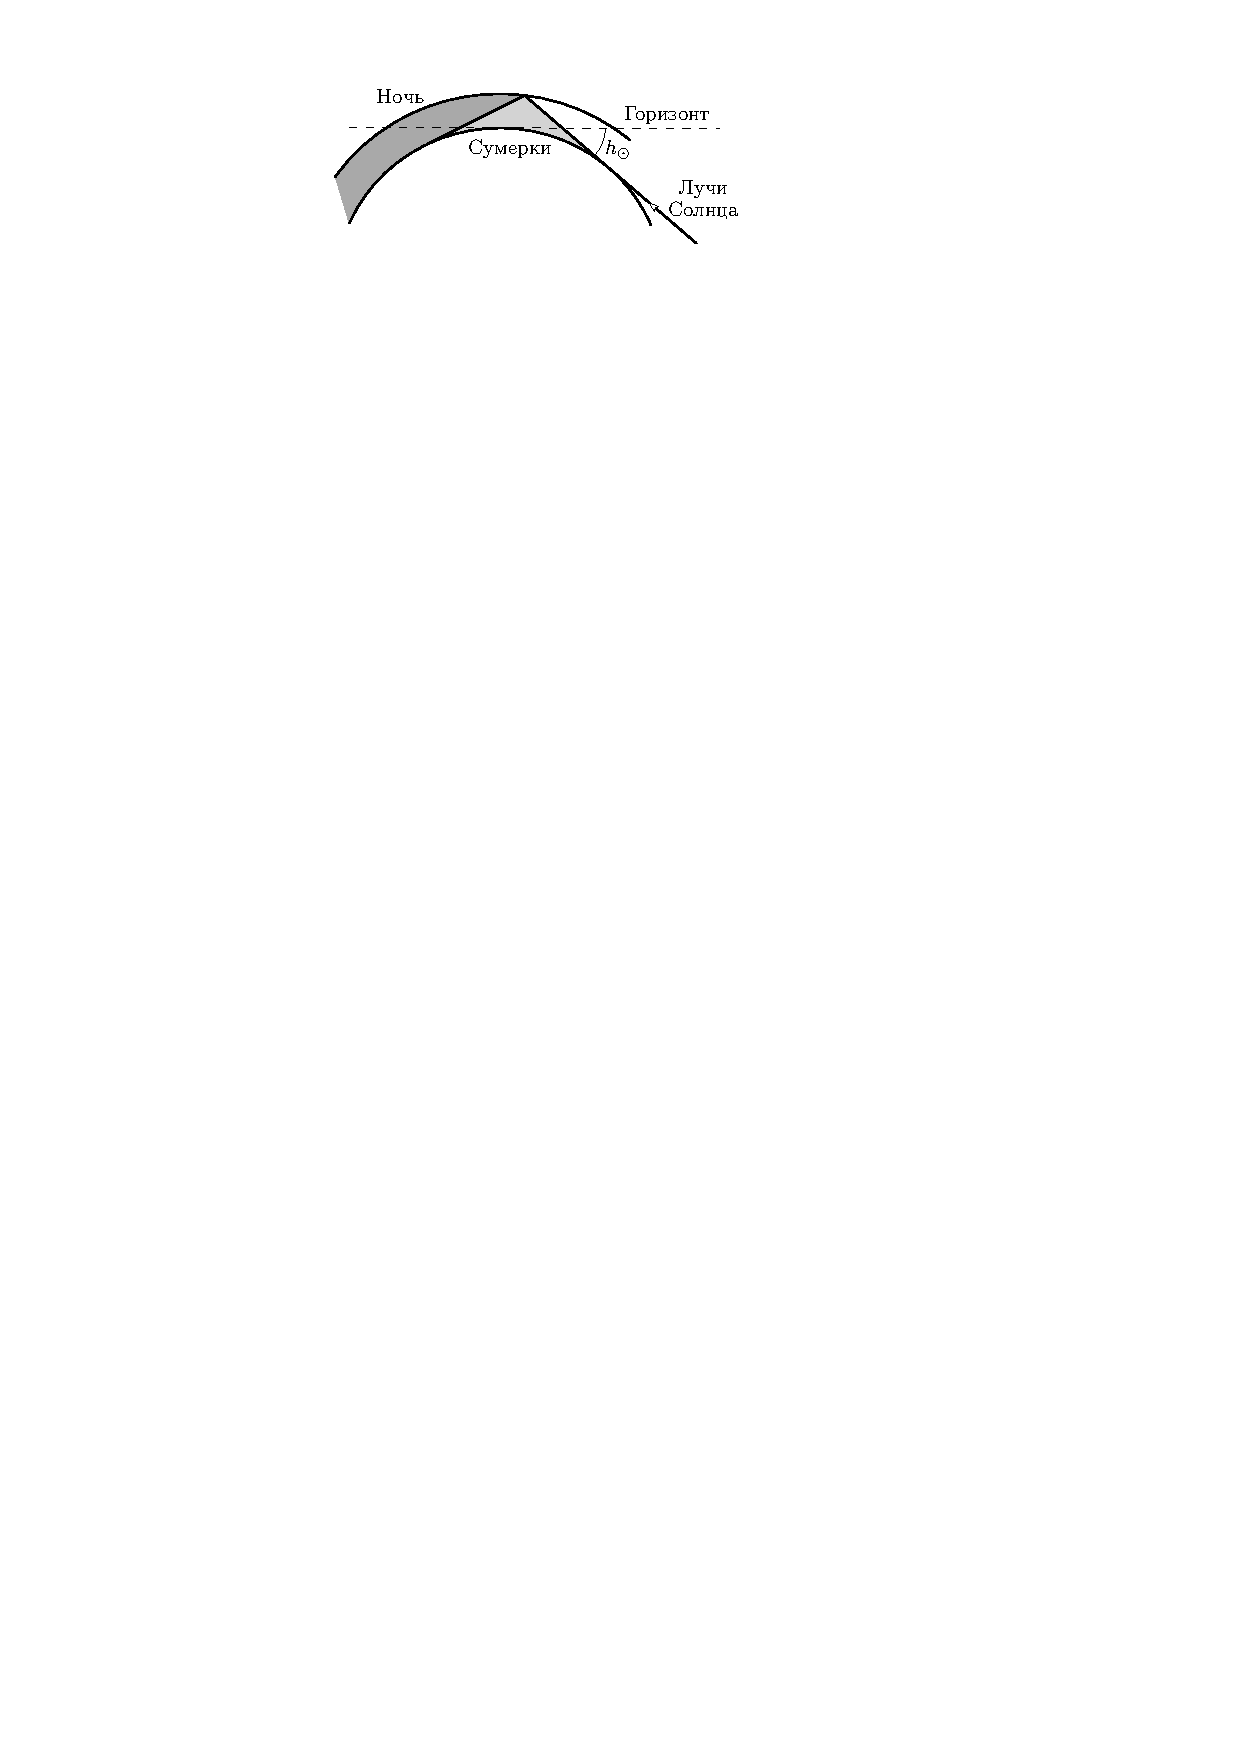
\includegraphics[width=\tw]{spher-astro-dusk.pdf}
	\captionof{figure}{Сумерки}
\end{minipage}
\newpage


	\section{Объекты космоса}
\subsection{Солнце}
\term{Солнце} --- центральное тело Солнечной системы, в нём сосредоточено 99,866\%  всей массы. Водород составляет~73\% общей массы Солнца, гелий~---~25\%. Остальные элементы: кислород, углерод, азот, магний, кремний, железо, сера, алюминий, натрий, кальций, никель и другие дают вклад всего~2\%.

По спектральной классификации Солнце~--- звезда типа G2V (жёлтый карлик на главной последовательности). Температура поверхности Солнца составляет $5 778$~К, поэтому Солнце светит почти в белом свете, но прямой свет Солнца у поверхности Земли приобретает жёлтый оттенок из-за рассеяния и поглощения коротковолновой части спектра в атмосфере.

Солнце вырабатывает энергию путём термоядерного синтеза. Каждую секунду в ядре около 4~млн.~тонн вещества превращается в лучистую энергию.\\

\term{Строение Солнца.}~~~В центре Солнца находится ядро с радиусом $150 $ -- $ 180$~тыс.~км, где идут термоядерные реакции. Плотность ядра около $1.5\times 10^5~\text{кг}/\text{м}^3$, а температура в его центре достигает $1.5\times 10^7$~К.

\begin{figure}[h!]
	\centering
	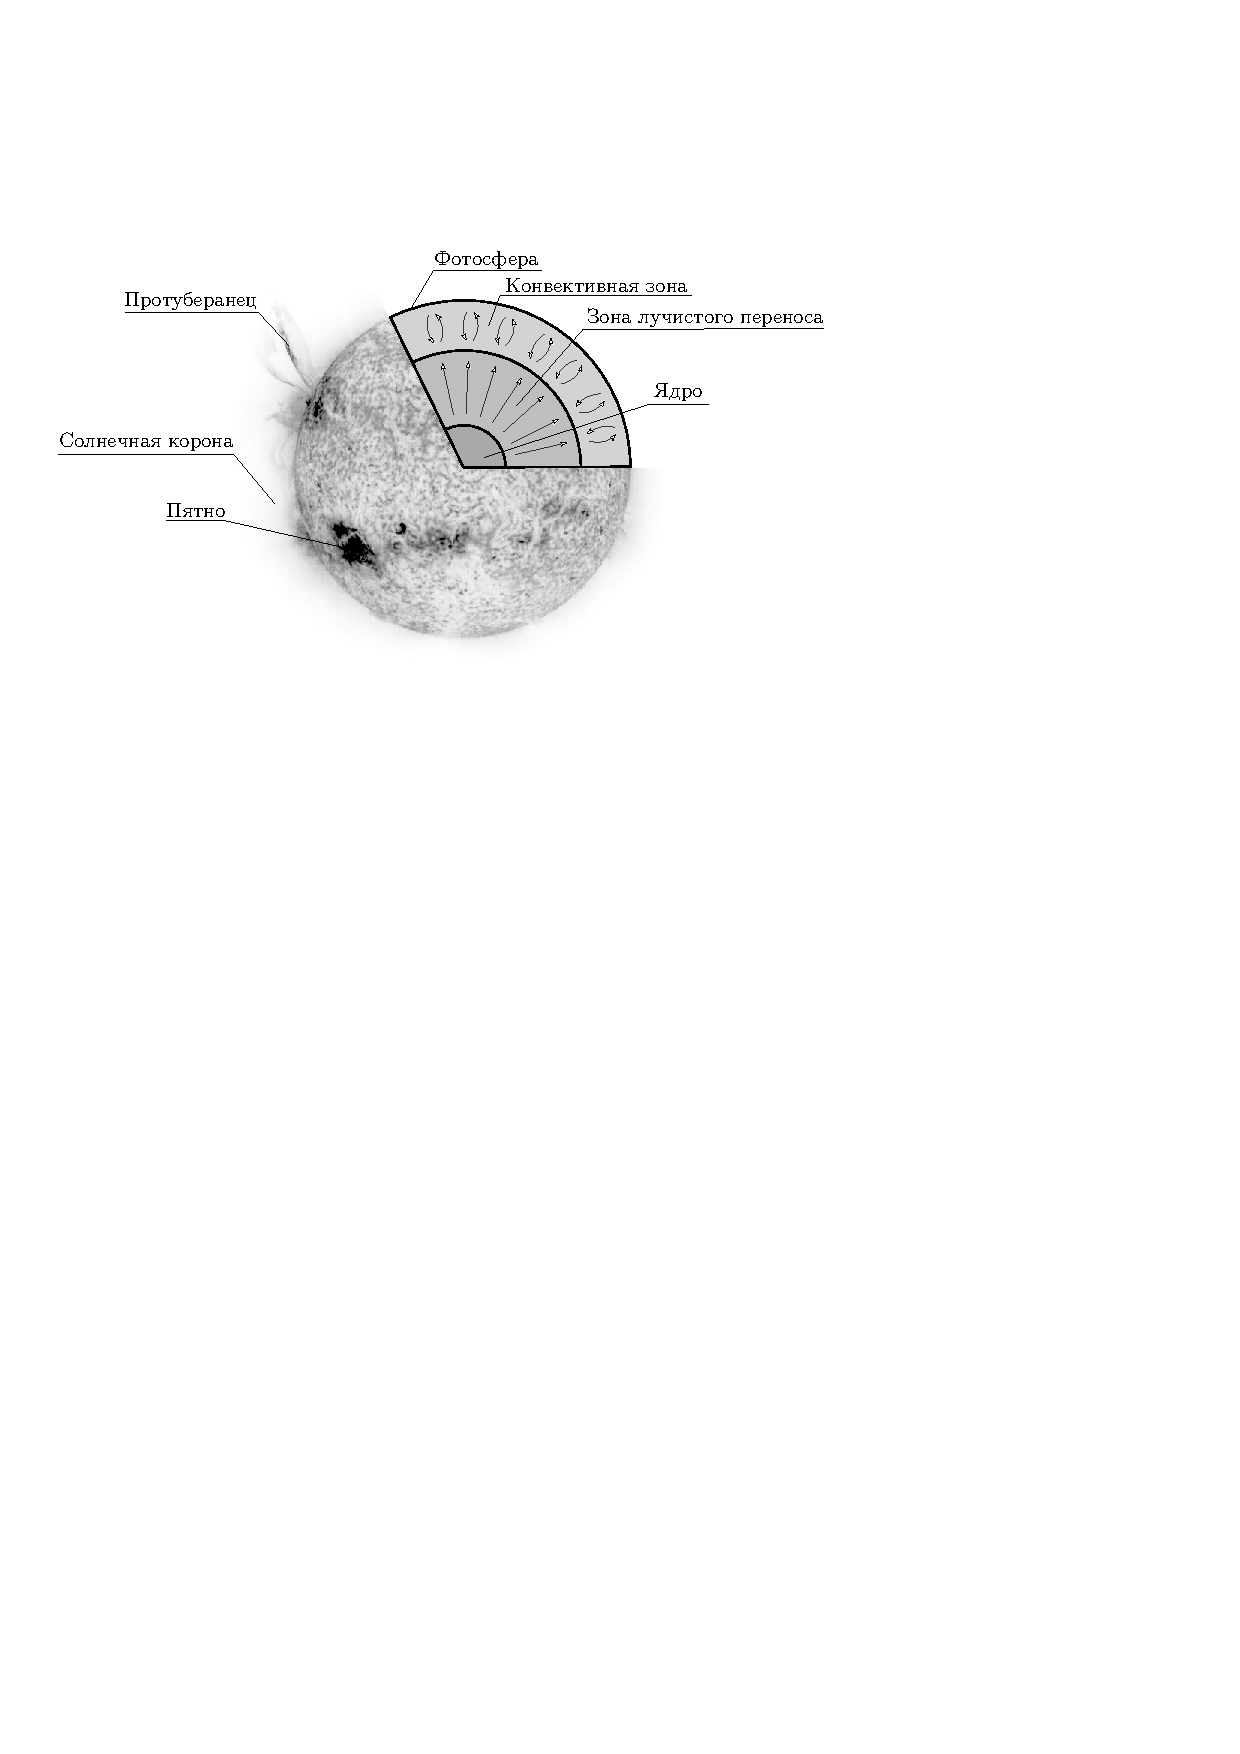
\includegraphics[width=0.8\textwidth]{sun.pdf}
	\caption{Строение Солнца. Фотография со спутника1 SOHO в фильтре $H_\alpha$ (негатив)}
\end{figure}
Над ядром, на расстояниях примерно от $0.25 R_\odot$ до $0.7R_\odot$ от его центра, находится \imp{зона лучистого переноса}. В этой зоне перенос энергии происходит главным образом с помощью излучения и поглощения фотонов. Температура в этой зоне лежит в интервале от $2\times10^6$~К сверху до $7\times10^6$~К снизу.

Над зоной лучистого  переноса (радиоактивная зона) находится \imp{конвективная зона}. Это слой толщиной примерно $2\times10^5$~км, в котором перенос энергии к поверхности совершается движением самого вещества. При приближении к поверхности конвективной зоны температура падает до $~5800$~К.

\textit{Фотосфера} --- видимая поверхность Солнца, по которой определяется размер Солнца. Эффективная температура фотосферы $T_\odot =  5778$~К.

\textit{Хромосфера} --- внешняя оболочка Солнца толщиной около 2000 км, окружающая фотосферу. Из хромосферы происходят горячие  выбросы вещества --- \textit{спикулы}. Температура хромосферы увеличивается с высотой до $2\times10^4$~К.

\textit{Солнечная корона} --- последний внешний слой Солнца, который состоит из протуберанцев и энергетических  извержений, образующих солнечный ветер. Средняя температура короны $2 \times 10^6$~К, а в некоторых частях достигает  и $20\times10^6$~К. Столь высокая температура обусловлена процессами, происходящими в магнитном поле звезды. Однако, несмотря на столь высокую температуру, корона видна лишь во время солнечных затмений, так как плотность её очень мала.

\term{Вращение Солнца} происходит не твердотельно~--- угловая скорость на разных широтах отличается, при удалении от экватора она уменьшается. Период вращения Солнца на разных широтах можно найти, наблюдая за солнечными пятнами и другими образованиями в фотосфере звезды. На экваторе период вращения составляет 25.05 суток, к полюсу он увеличивается до 34 суток. По наблюдениям за пятнами в течение длительного периода при помощи метода наименьших квадратов можно найти зависимость углового перемещения пятна за сутки от гелиографической широты:
\begin{equation}
	\Delta\lambda=14.37^{\circ}-2.7^{\circ}\sin^2\varphi,
\end{equation}
где $\Delta\lambda$~--- угловое перемещение пятна, $\varphi$~--- гелиографическая широта. Данная зависимость верна только для широт $\varphi < 40^\circ$.

\subsection{Спектральные классы звёзд}
\begin{table}[h!]
	\centering
	\footnotesize
	\renewcommand{\arraystretch}{1.4}
	\renewcommand{\tabcolsep}{0pt}
	\begin{tabularx}{\tw}{|C{0.1}|C{0.3}|C{0.23}|C{0.13}|C{0.13}|C{0.13}|}
		\hline
		{\bfseries Класс} & {$\mathbf{T}$, К} & {\bfseries Цвет} & {$\mathbf{M}$, $M_{\odot}$} & {$\mathbf{R}$, $R_{\odot}$} & {$\mathbf{L}$, $L_{\odot}$}\\
		\hline
		O & $3 \times 10^4$ --- $6 \times 10^4$ & Голубой & 60 & 15 & $1.4 \times 10^6$\\
		
		B & $1 \times 10^4$ --- $3 \times 10^4$ & Бело-голубой & 18 & 7 & $2 \times 10^4$\\
		
		A & $7.5 \times 10^3$ --- $1 \times 10^4$ & Белый & 3.1 & 2.1 & 80\\
		
		F & $6 \times 10^3$ --- $7.5 \times 10^3$ & Жёлто-белый & 1.7 & 1.3 & 6\\
		
		G & $5 \times 10^3$ --- $6 \times 10^3$ & Жёлтый & 1.1 & 1.1 & 1.2\\
		
		K & $3.5 \times 10^3$ --- $5 \times 10^3$ & Оранжевый & 0.8 & 0.9 & 0.4\\
		
		M & $2 \times 10^3$ --- $3.5 \times 10^3$ & Красный & 0.3 & 0.4 & 0.04\\
		\hline
	\end{tabularx}
	\caption{Современная спектральная классификация звёзд}
	\label{tab:spectr-types}
\end{table}
Звёзды в зависимости от своего цвета делятся на \imp{спектральные классы}, основные из них представлены в Таблице\,\ref{tab:spectr-types}. Масса, радиус и светимость приведены средних представителей спектрального класса, лежащих на главной последовательности (V).

Запись спектрального класса представляет собой латинскую букву, арабское число и римское число, например, спектральный класс Солнца~--- G2V. арабское число показывает к какой именно части спектрального класса относится звезда: к более синей (число меньше) или к красной (число больше). Так,~G10V~--- это тоже самое, что K0V. Спектральный класс (показатель цвета) и абсолютная звёздная величина задают положение звезды на \imp{Диаграмме Герцшпрунга-Рассела}.

\begin{figure}[h!]
	\centering
	\vspace{-1pc}
	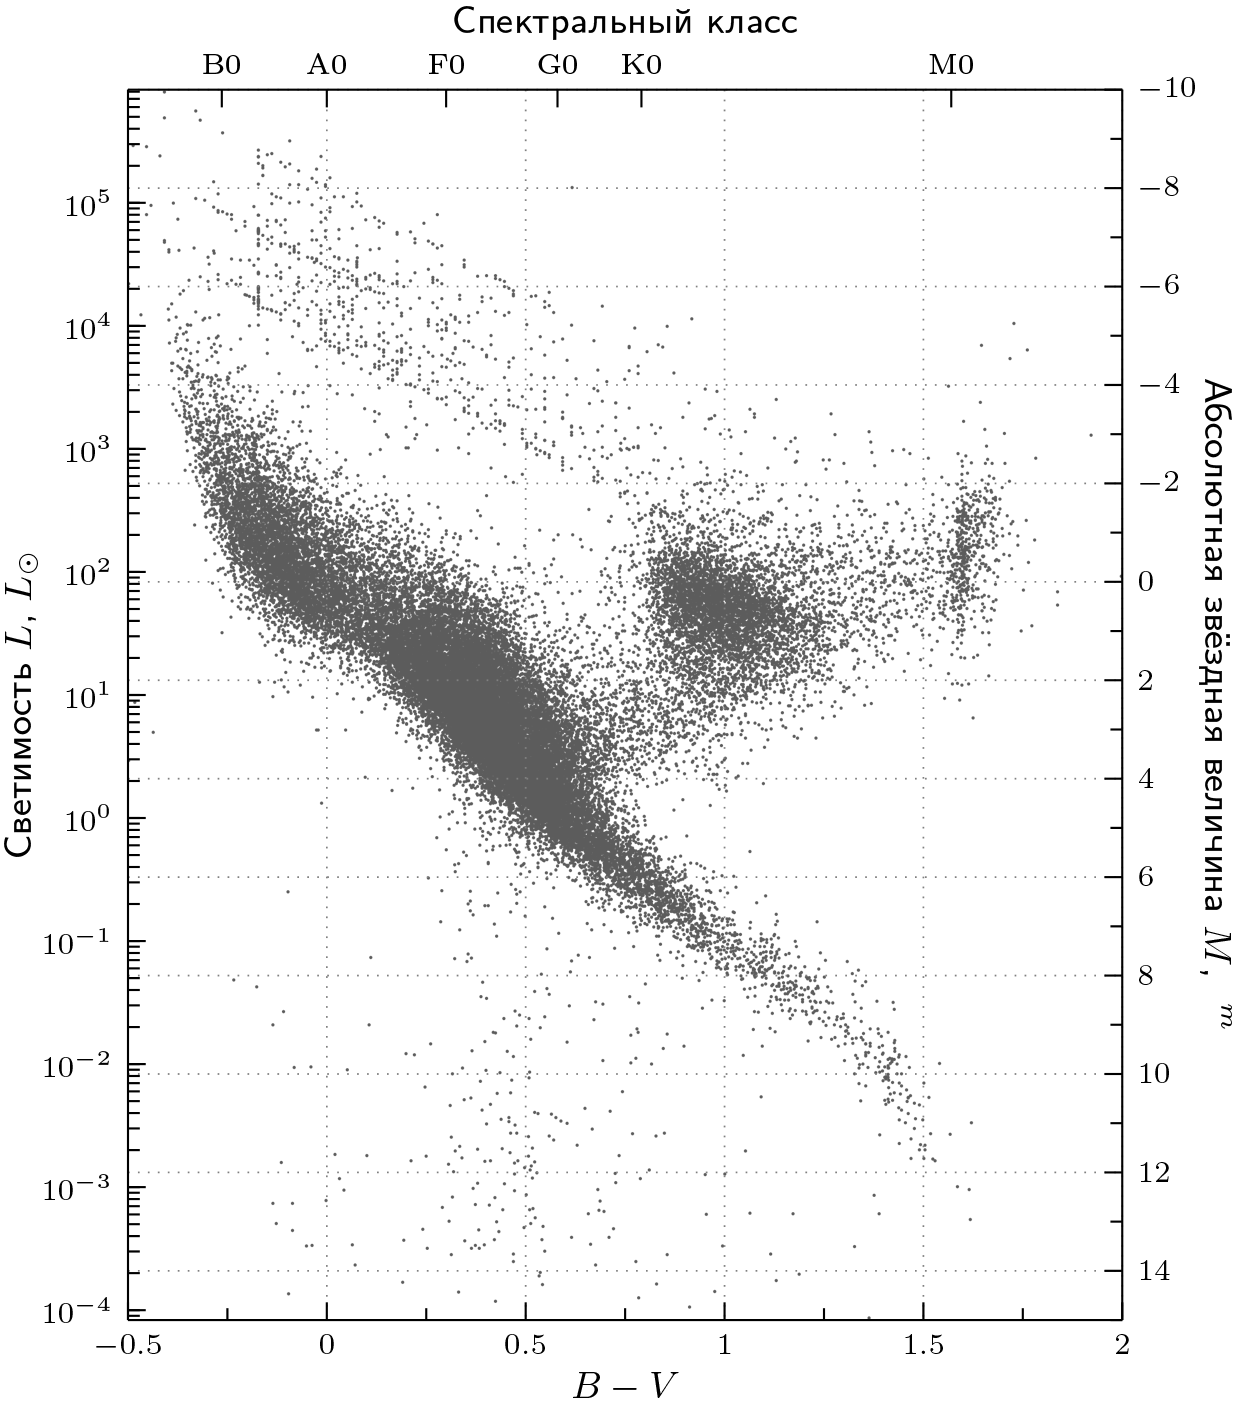
\includegraphics[width=10cm]{gr}
	\caption{Диаграмма Герцшпрунга--Рассела}
	\label{pic:d-cep}
\end{figure}
\term{Диаграмма Герцшпрунга-Рассела} показывает зависимость светимости или абсолютной звёздной величины от спектрального класса, показателя цвета $(B-V)$ или эффективной температуры фотосферы звезды.

Была предложена примерно в 1910 году независимо Эйнаром Герцшпрунгом и Генри Расселом. Диаграмма используется для классификации звёзд и соответствует современным представлениям о звёздной эволюции.

Около $90 \%$ звёзд находятся на главной последовательности. Их светимость обусловлена термоядерными реакциями превращения водорода в гелий. Выделяется также несколько ветвей проэволюционировавших звёзд-гигантов, в которых происходит горение гелия и более тяжёлых элементов. В левой нижней части диаграммы находятся полностью проэволюционировавшие белые карлики.

Мнемонические правила для запоминания спектральных классов: <<\textbf{O}h \textbf{B}e \textbf{A} \textbf{F}ine \textbf{G}irl, \textbf{K}iss \textbf{M}e \textbf{R}ight \textbf{N}ow \textbf{S}weetheart.>> и <<\textbf{В}ообразите: \textbf{О}дин \textbf{Б}ритый \textbf{А}нгличанин \textbf{Ф}иники \textbf{Ж}евал \textbf{К}ак \textbf{М}орковь --- \textbf{Р}азве \textbf{Н}е \textbf{С}мешно?>>

%	\begin{tikzpicture}
% 		\begin{axis}[
% 						height	=	12cm,
% 						width	=	10cm,
% 						ymax	=	15.,
% 						ymin	=	-10.,
% 						y dir	=	reverse,
% 						xmax	=	2.,
% 						xmin	=	-.5,
% 						axis x line* = bottom,
% 						axis y line* = right,
% 						xlabel=$B-V$,
% 						y label style = {at={(axis description cs: 1.2, 0.5)}, rotate=180},
% 						ylabel	=	{Абсолютная звёздная величина $M$, $~^m$}
% 					]
%%			\addplot+[only marks, mark = o, mark options={scale=0.2, black}] table[x=f, y=m]{data/light-curve-D-Cep.txt};
% 		\end{axis}
% 		\begin{semilogyaxis}[
% 						height	=	12cm,
% 						width	=	10cm,
% 						ymax	=	8.312e5,
% 						ymin	=	8.312e-5,
% 						xmax	=	2.,
% 						xmin	=	-.5,
% 						minor x tick num = 0,
% 						minor y tick num = 01,
% 						xtick = {-0.264, 0, 0.3, 0.58, 0.791, 1.57},
% 						xticklabels = {B0, A0, F0, G0, K0, M0},
% 						axis x line* = top,
% 						axis y line* = left,
% 						xlabel	=	{Спектральный класс},
% 						x label style = {at={(axis description cs: 0.5, 1.11)}, rotate=0},
% 						ylabel	=	{Светимость $L$, $L_\odot$},
% 						ymajorgrids	 =	false,
% 						xmajorgrids	 =	false
%    				]
%		\end{semilogyaxis}
% 	\end{tikzpicture}
Помимо основных спектральных классов звёзд существуют дополнительные: W~--- звёзды Вольфа-Райе, очень тяжёлые яркие звёзды с температурой порядка $70000$~К и интенсивными эмиссиоными линиями спектра; L~--- звёзды или коричневые карлики с температурой 1500\,--\,2000~К и соединениями металлов в атмосфере; T~--- метановые коричневые карлики с температурой $700 - 1500$~К; Y~---  очень холодные (метано-аммиачные) коричневые карлики с температурой ниже $700$~К; C~--- углеродные звёзды, гиганты с повышенным содержанием углерода. Ранее относились к классам R и N.

\subsection{Переменные звёзды}
\term{Переменные звёзды}~--- звёзды, у которых наблюдаются колебания блеска.   Для отнесения звезды к разряду переменных достаточно, чтобы блеск звезды хотя бы однажды претерпел изменение.

Переменные звёзды делятся на две большие группы: \imp{затменные} и \imp{физические}, причём физические подразделяются на \imp{пульсирующие} и \imp{эруптивные}.

\begin{wrapfigure}[11]{l}{0.5\tw}
	\centering
	\vspace{-1.2pc}
	\begin{tikzpicture}
		\begin{axis}[
			height	=	4.5cm,
			width	=	.5\tw,
			xlabel	=	{Фаза},
			ylabel	=	{Блеск $m$, $~^m$},
			ymax	=	8.,
			ymin	=	6.5,
			y dir	=	reverse,
			xmax	=	1,
			xmin	=	0
			]
			\addplot+[only marks, mark = o, mark options={scale=0.2, black}] table[x=f, y=m]{data/light-curve-D-Cep.txt};
		\end{axis}
	\end{tikzpicture}
	\caption{Кривая блеска переменной типа $\delta$\,Cep}
	\label{pic:d-cep}
\end{wrapfigure}
К \term{пульсирующим} переменным  относят те звёзды, переменность которых вызвана процессами, происходящими в их недрах. Эти процессы приводят к периодическому изменению температуры поверхности и радиуса фотосферы, а вместе с ними и блеска звезды. Период переменности варьируется в пределе от долей суток до~нескольких~лет в зависимости от типа переменной.

Классический пример пульсирующих переменных звёзд~--- \imp{цефеиды}, названные в честь первой открытой переменной данного типа~--- $\delta$\,Cep. Абсолютную звёздную величину $M$ и период $T$ (в сутках) цефеид связывает соотношение
\begin{equation}
	M = -1.43^m - 2.81\lg T.
\end{equation}
К \term{эруптивным} переменным звёздам относятся звёзды, меняющие свой блеск нерегулярно или единожды за время наблюдений. Все изменения блеска эруптивных звёзд связывают с бурными процессами и вспышками в их хромосферах и коронах. К таким, например, относятся \imp{новые} и \imp{сверхновые}.

\term{Затменно-переменные} звёзды --- системы из двух звёзд, суммарный блеск которых периодически изменяется с течением времени. Причиной изменения блеска могут быть затмения звёзд друг другом, или изменение их формы взаимной гравитацией в тесных системах. На Рис.\,\ref{pic:w-uma}\,--\,\ref{pic:b-lyr}  представлены кривые блеска затменно-переменных звёзд трёх основных типов.

\begin{figure}[!h]
	\centering
	\begin{minipage}[c]{0.49\tw}
		\begin{tikzpicture}
			\begin{axis}[
				height	=	4.5cm,
				width	=	\tw,
				xlabel	=	{Фаза},
				ylabel	=	{Блеск $m$, $~^m$},
				ymax	=	1.1,
				ymin	=	-.1,
				y dir	=	reverse,
				xmax	=	1,
				xmin	=	0
				]
				
				\addplot[smooth] table[x=t, y=m]{data/light-curve-W-UMa.txt};
			\end{axis}
		\end{tikzpicture}
	\end{minipage}
	\hfill
	\begin{minipage}[c]{0.49\tw}
		\centering
		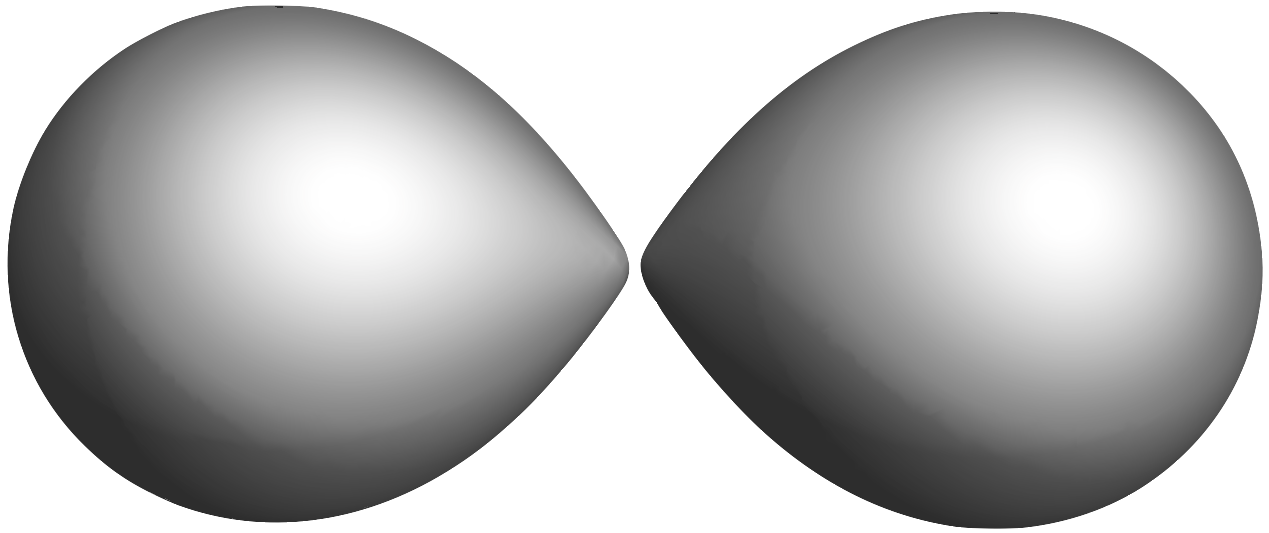
\includegraphics[width = .9\tw]{w-uma}
	\end{minipage}
	\caption{Кривая блеска переменной типа W\,UMa}
	\label{pic:w-uma}
\end{figure}

\begin{figure}[!h]
	\centering
	\begin{minipage}[c]{0.49\tw}
		\begin{tikzpicture}
			\begin{axis}[
				height	=	4.5cm,
				width	=	\tw,
				xlabel	=	{Фаза},
				ylabel	=	{Блеск $m$, $~^m$},
				ymax	=	.7,
				ymin	=	-.1,
				y dir	=	reverse,
				xmax	=	1.,
				xmin	=	.0
				]
				\addplot[smooth] table[x=t, y=m]{data/light-curve-B-Per.txt};
			\end{axis}
		\end{tikzpicture}
	\end{minipage}
	\hfill
	\begin{minipage}[c]{0.49\tw}
		\centering
		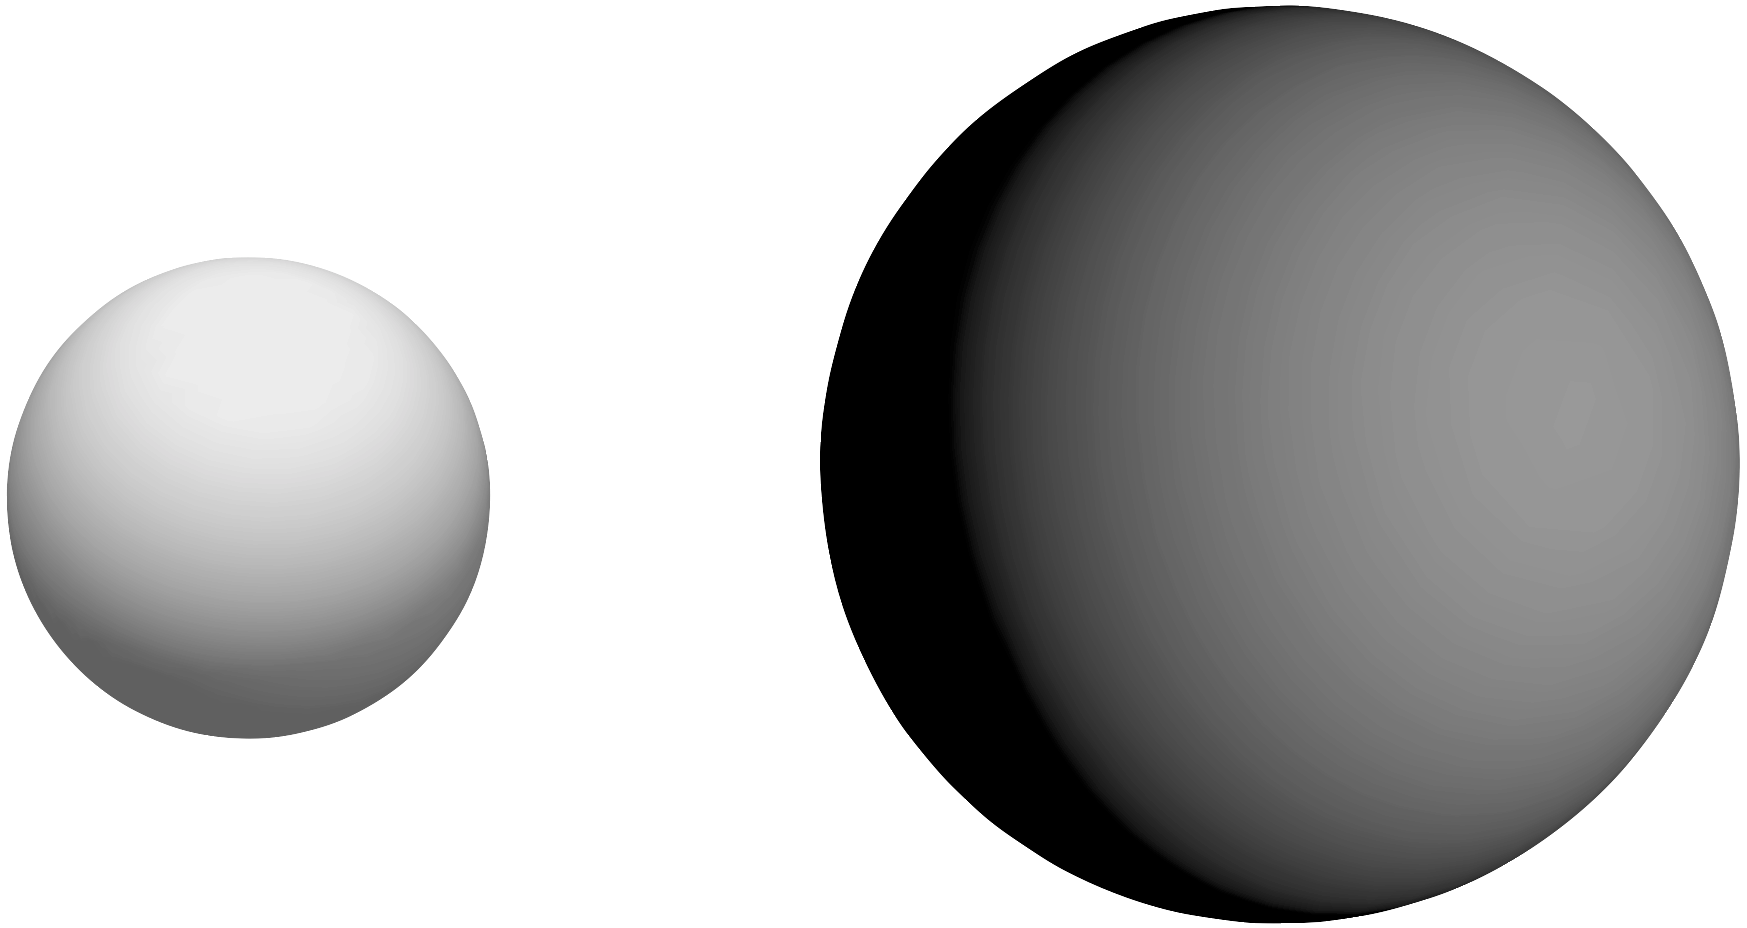
\includegraphics[width=.9\tw]{b-per}
	\end{minipage}
	\caption{Кривая блеска переменной типа $\beta$\,Per}
\end{figure}

\subsection{Вырожденные звёзды}
\term{Вырожденные звезды}~--- звезды, в которых силам гравитации противостоят силы давление вырожденного газа. К таким относятся \imp{белые карлики} и \imp{нейтронные звезды}. 

\begin{figure}[!h]
	\centering
	\begin{minipage}[c]{0.49\tw}
 		\begin{tikzpicture}
 			\begin{axis}[
 							height	=	4.5cm,
 							width	=	\tw,
 							xlabel	=	{Фаза}, 
 							ylabel	=	{Блеск $m$, $~^m$}, 
 							ymax	=	.7,
 							ymin	=	-.1,
 							y dir	=	reverse,
 							xmax	=	1,
 							xmin	=	.0
 						]
				\addplot[smooth] table[x=t, y=m]{data/light-curve-B-Lyr.txt};
 			\end{axis}
 		\end{tikzpicture}
 	\end{minipage}
 	\hfill
 	\begin{minipage}[c]{0.49\tw}
 		\centering
 		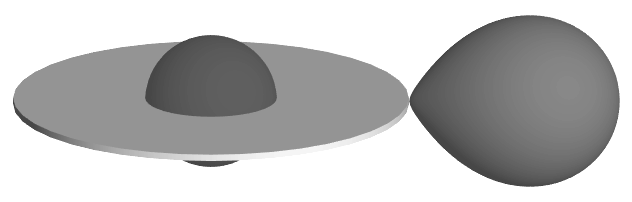
\includegraphics[width = .9\tw]{b-lyr}	
 	\end{minipage}
 	\caption{Кривая блеска переменной типа $\beta$\,Lyr}
 	\label{pic:b-lyr}
 	\vspace{-.8pc}
\end{figure}
\term{Белые карлики}~--- проэволюционировавшие звёзды лишённые собственных источников термоядерной энергии. Масса белого карлика находится в диапазоне от $0.6M_{\odot}$ до $1.44 M_{\odot}$. Верхняя границы массы белого карлика называется пределом Чандрасекара, звезда с массой больше данного предела не может существовать как белый карлик. Радиус белых карликов примерно в $10^2$ раз меньше солнечного, т.е. можно считать, что $R_\text{БК} \simeq R_\oplus$. Плотность белых карликов лежит в диапазоне $10^7$\,--\,$10^{10}$~$\text{кг}/\text{м}^3$.

\term{Нейтронная звезда}~--- сверхплотная звезда, образующаяся в результате взрыва Сверхновой. Вещество нейтронной звезды состоит в основном из нейтронов. Масса нейтронной звезды лежит в пределах от $0.1M_{\odot}$ до $2$\,--\,$2.8M_{\odot}$ (предел Оппенгеймера-Волкова). Размер данной звезды составляет лишь $10$\,--\,$20$~км, а плотность составляет $10^{16}$\,--\,$10^{18}$ $\text{кг}/\text{м}^3$.  Дальнейшему гравитационному сжатию нейтронной звезды препятствует давление ядерной материи, возникающее за счёт взаимодействия нейтронов. Так как нейтронные звёзды образуются в результате  коллапса массивных звёзд, то из-за сохранения момента импульса скорость их вращения очень велика~--- максимальная скорость может достигать $10^5$~км/с.
\subsection{Чёрные дыры}
\term{Чёрная дыра}~(ЧД)~--- область пространства-времени с массой $M$, гравитационное притяжение которой настолько велико, что покинуть её не могут даже объекты, движущиеся со скоростью света $c$. Граница этой области называется \imp{горизонтом событий}, а её характерный размер~$R_G$~--- \imp{гравитационным радиусом}, для величины которого справедливо равенство
\begin{equation}
R_G = \frac{2 G M}{c^2}.
\end{equation}

Минимальная масса ЧД составляет около $2.5M_{\odot}$. А плотность ЧД определяется отношением ее массы~$M$ к~объему~$V$, следовательно
\begin{equation}
\rho = \frac{M}{V} = \frac{3c^6}{32\pi M^2G^3}.
\end{equation}

\term{Эффект излучения} (испарения) \term{Хокинга}~--- эффект, при котором гравитационное поле черной дыры поляризует вакуум, в результате чего возможно образование не только виртуальных, но и реальных пар частица~--античастица. Одна из частиц, оказавшаяся чуть ниже горизонта событий, падает внутрь чёрной дыры, а другая, оказавшаяся чуть выше горизонта, улетает, унося энергию (то есть часть массы) чёрной дыры. Для мощности излучения ЧД справедлива формула
\begin{equation}
L = \frac{h c^6}{30720 \pi^2 G^2 M^2},
\end{equation}
где $h$ --- постоянная Планка. Спектр хокинговского излучения для безмассовых полей оказался строго совпадающим с излучением абсолютно чёрного тела, что позволило приписать ЧД температуру, равную
\begin{equation}
T = \frac{h c^3}{16 \pi^2 k G M},
\end{equation}
где $k$ --- постоянная Больцмана.
\subsection{Галактики}
\term{Морфологическая классификация галактик}~--- система разделения галактик на группы по визуальным признакам, используемая в астрономии. Наиболее известной является классификация, разработанная Хабблом и дополненная другими учеными. 
	\begin{figure}[h!]
		\centering
		\vspace{-.9pc}
		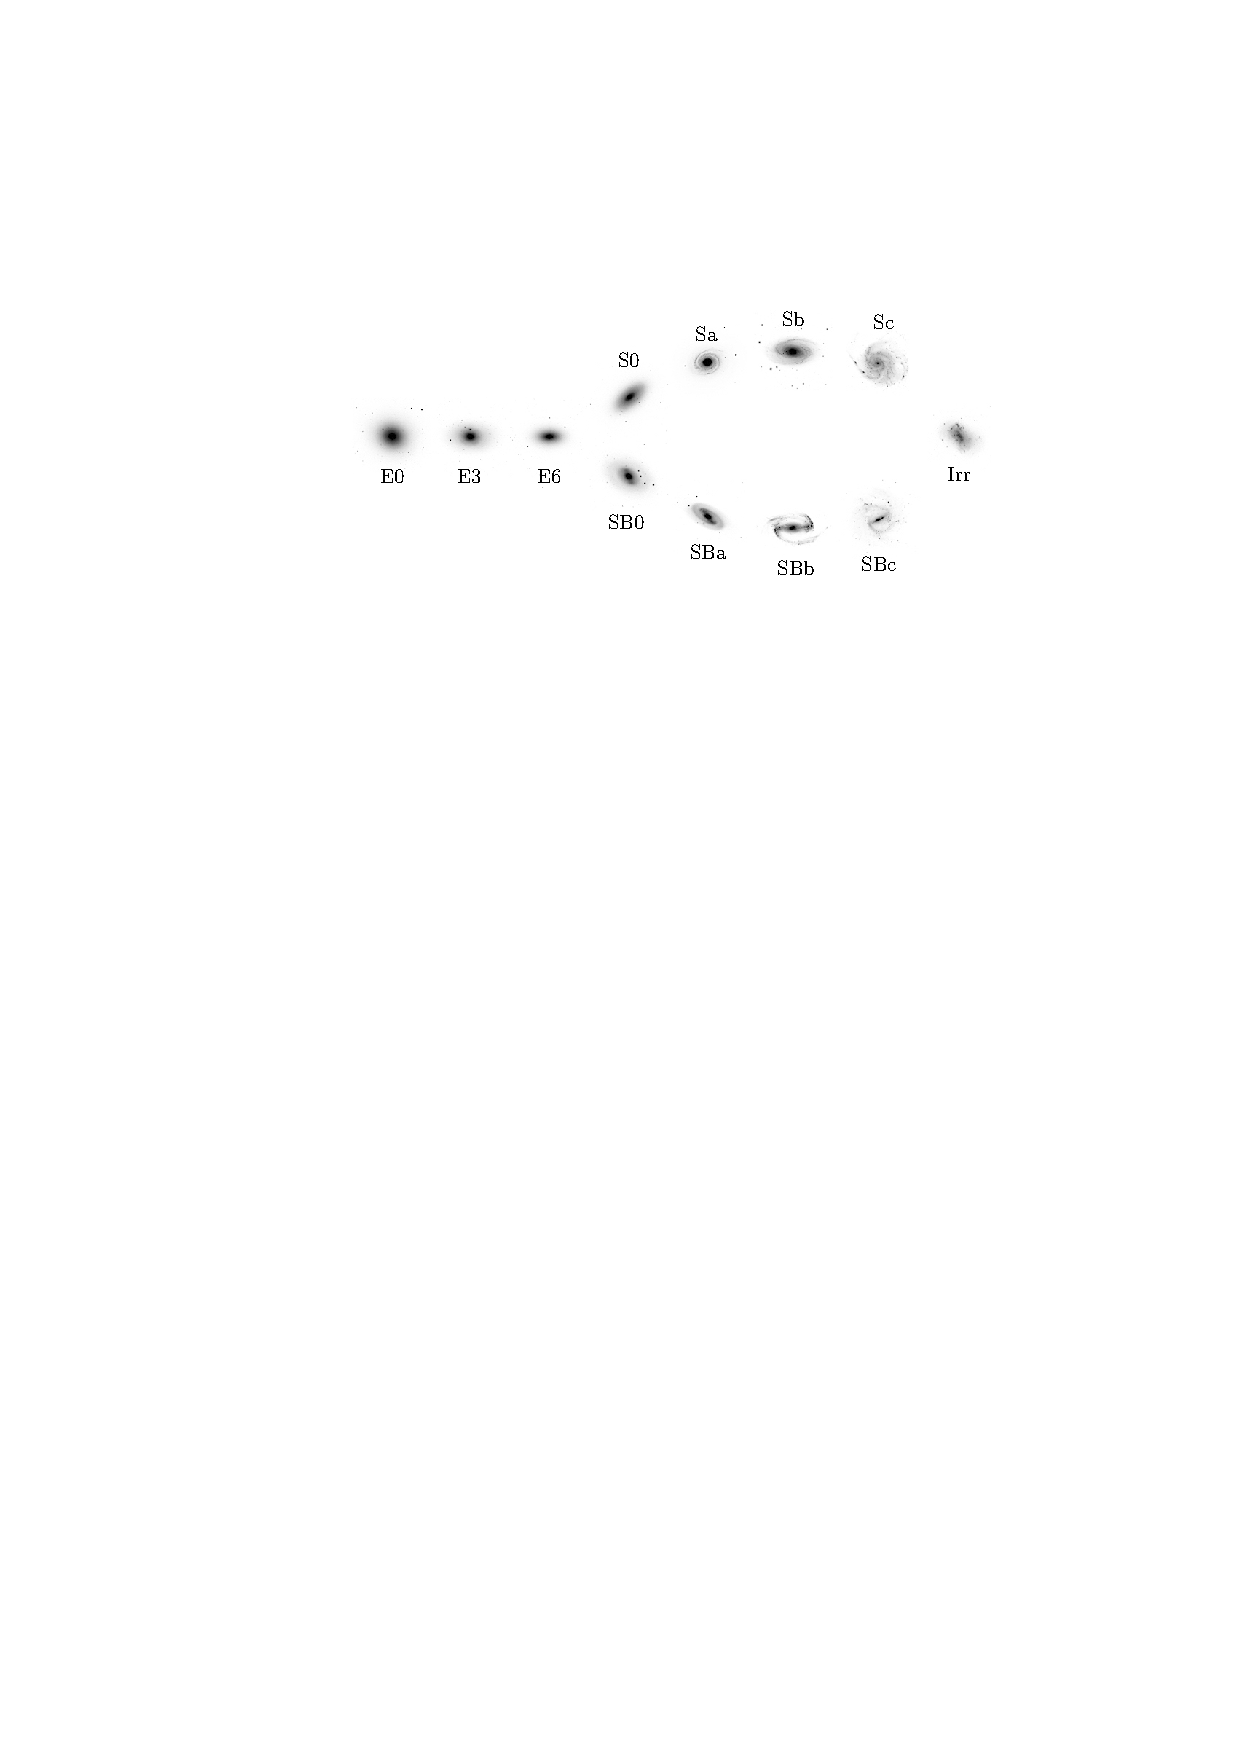
\includegraphics[width=0.65\tw]{hubble-fork.pdf}
		\caption{<<Вилка Хаббла>>}
	\end{figure}
	
Согласно данной классфикации галактики делятся на 4 типа:
\begin{enumerate}[itemsep=3pt, label={\arabic*.}, leftmargin=1pc]
	\item{\term{Эллиптические галактики} имеют гладкую эллиптическую форму без отличительных деталей с равномерным уменьшением яркости от центра к периферии. Обозначаются буквой E с индексом. Индекс можно рассчитать по формуле
		\begin{equation}
		i = 10 \cdot \left(1 - \frac{b}{a}\right),
		\end{equation}\nopagebreak
		где $a$ и $b$~--- большая и малая полуоси видимого эллипса. 
		
		К линзовидным галактикам с абсолютной звёздной величиной около $-21^m$ применимо соотношение Фабер-Джексона:
		\begin{equation}
			L \propto \sigma^4,
		\end{equation}
		где $\sigma$~--- дисперсия скоростей вещества в галактике.}
	\item{\term{Спиральные галактики} состоят из уплощенного диска из звезд и газа, в центре которого находится сферическое уплотнение, называемое балджем, а также обширного сферического гало. Спиральные галактики обозначаются SB при наличии бара (перемычки между рукавами) или S при отсутствии бара. В зависимости от размеров ядра и балджа галактики делят на 3 группы: a, b и c. Для галактик Sa характерен большой балдж, для галактик Sc~--- маленький. Галактики Sb представляют собой нечто среднее между галактиками Sa и Sc.
	
	Светимость спиральных галактик $L$ связана с их максимальной скоростью вращения $v_\text{макс}$ \term{соотношением Талли-Фишера}:
	\begin{equation}
		L \propto v_\text{макс}^4.
	\end{equation}
	Абсолютная звёздная величина Млечного пути $M_\text{MW} \simeq -21^m$.}
	\item{\term{Неправильные или иррегулярные галактики}~--- галактика, лишенная как вращательной симметрии, так и значительного ядра. Обозначение: Irr.}
	\item{\term{Линзовидные галактики}~--- галактики, являющиеся переходными между спиральными и эллиптическими. Обозначения: S0, SB0.}
\end{enumerate}


\subsection{Другие объекты}
\begin{minipage}{0.63\tw}
\term{Шаровое звёздное скопление}~--- скопление звёзд, состоящее из нескольких сотен тысяч светил, тесно связанных гравитацией. Млечный путь насчитывает около 160 шаровых звёздных скоплений. Диаметры шаровых скоплений составляют 20\,--\,60~пк, массы~--- $10^4$\,--\,$10^6$~солнечных.\par

\term{Планетарная туманность}~--- система из звезды, называемой ядром туманности, и симметрично окружающей ее светящейся газовой оболочки. Планетарные туманности образуются при сбросе внешних слоёв (оболочек) красных гигантов и сверхгигантов с массой от $0.8M_\odot$ до $8M_\odot$ на завершающей стадии их эволюции. Характерный размер~--- 1\,--\,2~св.\,лет.
\end{minipage}
\hfill
\begin{minipage}{0.32\tw}
	\centering
	\vspace{-1.2pc}
	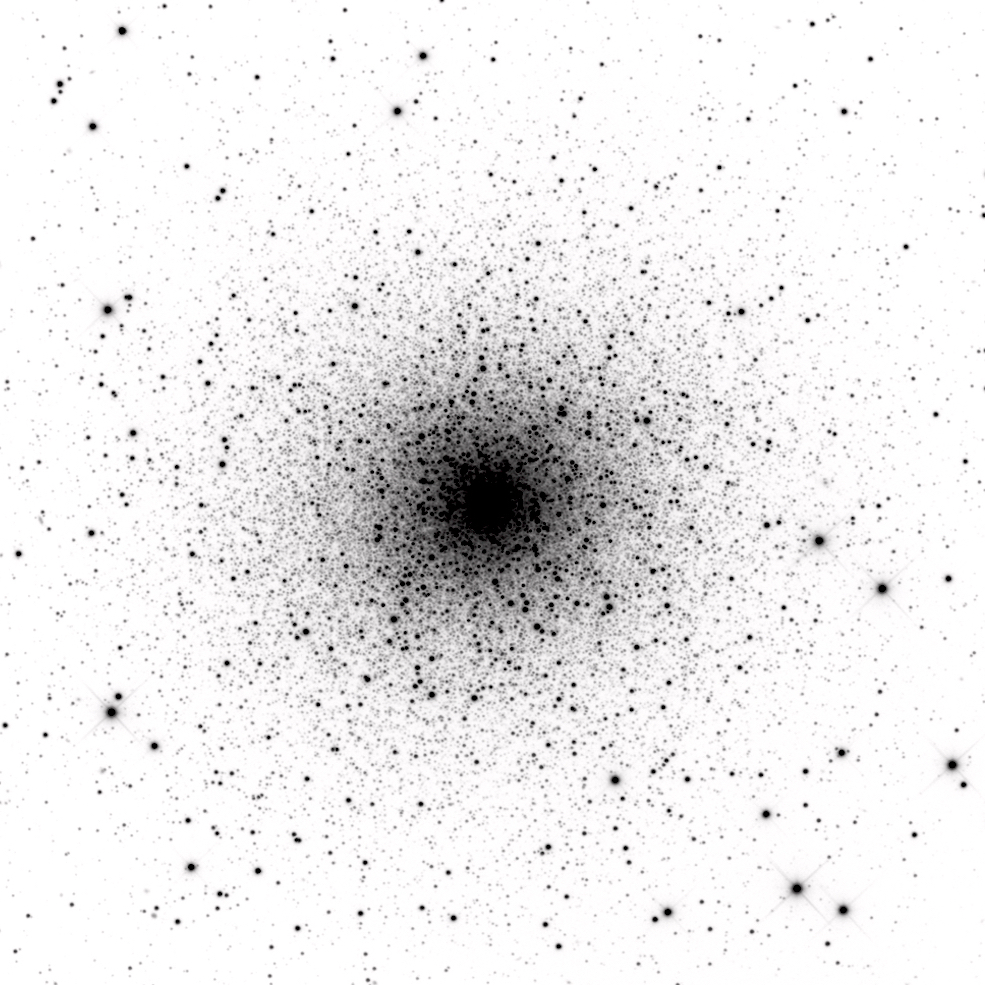
\includegraphics[width = .55\tw]{m13}
	\captionof{figure}{Шаровое скопление M13 (негатив)}
	\vspace{1pc}
	\includegraphics[width = .55\tw]{m57}
	\captionof{figure}{Пла\-не\-тар\-ная туманность M57 (негатив)}
\end{minipage}
	\newpage
\section{Математика}
\subsection{Системы координат}

\begin{wrapfigure}{r}{0.27\tw}
	\centering
	\vspace{-1pc}
	\begin{tikzpicture}[scale=1]
		\footnotesize
		\coordinate (O) at (0, 0);
		\coordinate (E1) at (2, 0);
		\coordinate (E2) at (1, 0.5);
		\coordinate (E3) at (0.5, 1.5);
		\coordinate (M) at (2, 2);
		
		\draw[semithick, -latex] (O) -- (E1);
		\draw[semithick, -latex] (O) -- (E2);
		\draw[semithick, -latex] (O) -- (E3);
		\draw[thick, -latex] (O) -- (M);
		
		\point (O);
		\point (M);
		
		\draw (1, 0) node[anchor=north]{$\vec{e}_1$};
		\draw (0.66, 0.33) node[anchor=north]{$\vec{e}_2$};
		\draw (0.25, 0.75) node[anchor=east]{$\vec{e}_3$};
		\draw (1, 1.05) node[anchor=south]{$\vec{r}$};
		\draw (M) node[anchor=north west]{$M$};
		\draw (O) node[anchor=north east]{$O$};
	\end{tikzpicture}
	\caption{}
	\vspace{-1pc}
	\label{pic:math-coord-sys-decart}
\end{wrapfigure}
Зафиксируем точку $O$ в пространстве и рассмотрим произвольную точку $M$. Вектор $\vec{r} = \overrightarrow{OM}$ называется радиус-вектором точки $M$. Пусть в рассматриваемом пространстве также выбран базис $\{\vec{e}_1, \ldots, \vec{e}_n \}$, тогда совокупность точка $O$ и базиса называется \term{декартовой системой координат}. Причем точка $O$~--- начало координат, а базисные векторы $\vec{e}_1, \ldots, \vec{e}_n$ задают координатные оси.

\begin{wrapfigure}{r}{0.27\tw}
	\centering
	\vspace{-1pc}
	\begin{tikzpicture}[scale=1]
		\footnotesize
		\coordinate (O) at (0, 0);
		\coordinate (E1) at (1.5, 0);
		\coordinate (E2) at (-1, -0.5);
		\coordinate (E3) at (0, 1.5);
%		\coordinate (M) at (2, 2);
		
		\draw[semithick, -latex] (O) -- (E1);
		\draw[semithick, -latex] (O) -- (E2);
		\draw[semithick, -latex] (O) -- (E3);
%		\draw[thick, -latex] (O) -- (M);
		
		\point (O);
%		\point (M);
		
		\draw (-0.5, -0.25) node[anchor=south]{$\vec{e}_1$};
		\draw (0.75, 0) node[anchor=south]{$\vec{e}_2$};
		\draw (0, 0.75) node[anchor=east]{$\vec{e}_3$};
%		\draw (1, 1.05) node[anchor=south]{$\vec{r}$};
%		\draw (M) node[anchor=south]{$M$};
		\draw (0, -0.1) node[anchor=north]{$O$};
		
		\draw (0, 0.25) -- (0.25, 0.25) -- (0.25, 0);
		\draw (0.25, 0) -- (0.027, -0.112) -- (-0.223, -0.112);
		\draw (0, 0.25) -- (-0.223, 0.138) -- (-0.223, -0.112);
	\end{tikzpicture}
	\caption{}
	\vspace{-1pc}
	\label{pic:math-coord-sys-ord-basis}
\end{wrapfigure}
Однако пользоваться представлением векторов в произвольном базисе довольно сложно, поэтому рассмотрим специальный тип~--- \term{орто\-нор\-ми\-рованный базис}~--- это такой базис, базисные векторы которого попарно ортогональны, и длина каждого равна единице.

\term{Прямоугольной декартовой системой координат} (ПДСК) называют декартову систему координат с ортонормированным базисом. В практических задачах использовать ПДСК не всегда удобно, поэтому также рассмотрим другие системы координат. 

\begin{wrapfigure}{r}{0.27\tw}
	\centering
	\vspace{-1pc}
	\begin{tikzpicture}[scale=1]
		\clip(-1.05, -1.55) rectangle (2.1, 1.55);
	
		\footnotesize
		\coordinate (O) at (0, 0);
		\coordinate (E1) at (2, 0);
%		\coordinate (E2) at (1, 0.5);
%		\coordinate (E3) at (0.5, 1.5);
		\coordinate (M) at (1, 1);
		
		\draw[semithick, -latex] (O) -- (E1);
%		\draw[semithick, -latex] (O) -- (E2);
%		\draw[semithick, -latex] (O) -- (E3);
		\draw[thick, -latex] (O) -- (M);
		\draw[-latex] (0.65, 0) arc(0:45:0.65);
		
		\foreach \r in {0.5, 1, 1.5} {
			\draw (O) circle(\r);
		};
		
		\point (O);
		\point (M);
		
		\draw (1.2, 0) node[anchor=north]{$\vec{r}_0$};
%		\draw (0.66, 0.33) node[anchor=north]{$\vec{e}_2$};
%		\draw (0.25, 0.75) node[anchor=east]{$\vec{e}_3$};
		\draw (0.5, 0.5) node[anchor=south]{$\vec{r}$};
		\draw (0.55, 0.3) node[anchor=west]{$\varphi$};
		\draw (1, 0.9) node[anchor=south east]{$M$};
		\draw (O) node[anchor=north east]{$O$};
	\end{tikzpicture}
	\caption{}
	\label{pic:math-coord-sys-polar}
\end{wrapfigure}
На плоскости, то есть в пространстве $\R^2$, имеющем размерность два, часто применяется \term{полярная система координат}. В ней координатами вектора является его длина $r$~--- расстояние до точки от начала отсчёта, и угол $\varphi$ радиус-вектора с начальной ось.

Пусть $(x,y)$~--- координаты некоторого вектора в ПДСК на $\R^2$, тогда не сложно получить, что его координаты в полярной системе координат (начальная ось совпадает с осью $Ox$)  удовлетворяют следующим соотношениям:
\begin{equation}
	\begin{cases}
		r = \sqrt{x^2 + y^2},\\
		\sin \varphi = y/r,\\
		\cos \varphi = x/r.
	\end{cases}
	\quad \Leftrightarrow \quad
	\begin{cases}
		x = r \cos \varphi,\\
		y = r \sin \varphi.
	\end{cases}
\end{equation}

\begin{wrapfigure}{r}{0.35\tw}
	\centering
%	\vspace{-1pc}
	\begin{tikzpicture}[scale=1]
		\clip(-1.3, -1.1) rectangle (2.5, 2.5);
	
		\footnotesize
		\coordinate (O) at (0, 0);
		\coordinate (E1) at (2.3, 0);
		\coordinate (E2) at (0, 2.3);
		\coordinate (E3) at (-1, -1);
		\coordinate (M) at (0.8, 1.3);
		\coordinate (M') at (0.8, -0.48);
		\coordinate (M'') at (1, -0.6);
		
		\draw[semithick, -latex] (O) -- (E1);
		\draw[semithick, -latex] (O) -- (E2);
		\draw[semithick, -latex] (O) -- (E3);
		\draw[thick, -latex] (O) -- (M);
		
		\draw [dashes] (0, 1.78) -- (M) -- (M');
		\draw [dashes] (M'') -- (O);
		\draw [dashes] (1.28, 0) -- (M') -- (-0.48, -0.48);
		
		\draw (O) ellipse(2 and 0.7);
		\draw (0, 1.78) ellipse(2 and 0.7);
		
		\draw [-latex](-0.2, -0.2) arc(-99.4:-75.76:1.22);

        \foreach \p in {O, M, M', M''} {
            \point (\p);
        };
		
		\draw (0.5, 0.65) node[anchor=south east]{$\vec{r}$};		
		\draw (0.05, -0.15) node[anchor=north]{$\varphi$};
		\draw (0.42, -0.2) node[anchor=west]{$r$};
		\draw (0.8, 0.4) node[anchor=west]{$h$};
		\draw (M) node[anchor=south west]{$M$};
		\draw (O) node[anchor=south east]{$O$};
		
		\draw (E1) node[anchor=north]{$y$};
		\draw (E2) node[anchor=east]{$z$};
		\draw (E3) node[anchor=east]{$x$};
	\end{tikzpicture}
	\caption{}
	\label{pic:math-coord-sys-cyl}
	\vspace{-2pc}
\end{wrapfigure}
Теперь пусть $(x, y, z)$~--- координаты некоторого вектора в ПДСК на~$\R^3$. Обозначим за $h$~--- длину проекции этого вектора на ось $z$, $r$~--- длину его проекции на плоскость $Oxy$, $\varphi$~--- угол между проекцией на плоскость $Oxy$ и осью $Ox$. Тогда тройка $(r, \varphi, h)$~--- координаты рассматриваемого векторы в \term{цилиндрической системе координат}, и верно представление
\begin{equation}
	\begin{cases}
		r = \sqrt{x^2 + y^2},\\
		\sin \varphi = y/r,\\
		\cos \varphi = x/r,\\
		h = z.
	\end{cases}
	\quad \Leftrightarrow \quad
	\begin{cases}
		x = r \cos \varphi,\\
		y = r \sin \varphi,\\
		z = h.
	\end{cases}
\end{equation}

\begin{wrapfigure}{r}{0.35\tw}
	\centering
	\vspace{-2.5pc}
	\begin{tikzpicture}[scale=1]
		\clip(-1.3, -1.1) rectangle (2.5, 2.5);
%	
%		\foreach \x in {-5, -4.9,...,5} {
%			\draw [line width=.1pt] (\x, -5) -- (\x, 5);
%		};
%		
%		\foreach \x in {-5, -4,..., 5} {
%			\draw [line width=.4pt] (\x , -5) -- (\x , 5);
%		};
%		
%		\foreach \y in {-5, -4,..., 5} {
%			\draw [line width=.4pt] (-5, \y) -- (5, \y);
%		};
%		
%		\foreach \y in {-5, -4.9,..., 5} {
%			\draw [line width=.1pt] (-5, \y) -- (5, \y);
%		};
	
		\footnotesize
		\coordinate (O) at (0, 0);
		\coordinate (E1) at (2.3, 0);
		\coordinate (E2) at (0, 2.3);
		\coordinate (E3) at (-1, -1);
		\coordinate (M) at (0.8, 1.3);
		\coordinate (M') at (0.8, -0.48);
		\coordinate (M'') at (1, -0.6);
		
		\draw[semithick, -latex] (O) -- (E1);
		\draw[semithick, -latex] (O) -- (E2);
		\draw[semithick, -latex] (O) -- (E3);
		\draw[thick, -latex] (O) -- (M);
		
		\draw [dashes] (0, 1.78) -- (M) -- (M');
		\draw [dashes] (M'') -- (O);
		\draw [dashes] (0, 2) arc(90:-90:1.05 and 2);
		\draw [dashes] (M') -- (-0.48, -0.48);
		\draw [dashes] (M') -- (1.28, 0);
%		\draw[-latex] (1.02, 0) arc(0:45:1 and 0.4);
		
		\draw (O) circle(2);
		\draw (0, 2) arc(90:270:0.7 and 2);
		\draw (2, 0) arc(360:180:2 and 0.7);
		
		\draw [-latex](-0.2, -0.2) arc(-99.4:-75.76:1.22);
		\draw [-latex](0.29, -0.18) arc(-9.44:18:1.22); 
%		\draw (O) ellipse(0.6 and 0.21);
%		\draw (-1, 0) circle(1.3);
		
		
		\foreach \p in {O, M, M', M''} {
            \point (\p);
        };
	
		
		\draw (0.5, 0.6) node[anchor=south east]{$\vec{r}$};		
%		\draw (1.05, -0.25) node[anchor=west]{$x$};
%		\draw (0.2, -0.45) node[anchor=north]{$y$};
%		\draw (0.75, 0.3) node[anchor=west]{$z$};
		\draw (0.3, 0.15) node[anchor=west]{$\varphi$};
		\draw (0.05, -0.15) node[anchor=north]{$\theta$};
		\draw (M) node[anchor=west]{$M$};
		\draw (O) node[anchor=south east]{$O$};
		
		\draw (E1) node[anchor=north]{$y$};
		\draw (E2) node[anchor=east]{$z$};
		\draw (E3) node[anchor=east]{$x$};
	\end{tikzpicture}
	\caption{}
	\label{pic:math-coord-sys-sphere}
	\vspace{-1.5pc}
\end{wrapfigure}
Остается рассмотреть \term{сферическую систему координат}. Здесь координатами точки будет длина $r$ радиус-вектора $\vec{r}$ и два угла: $\theta$~--- угол между радиус-вектором и плоскостью $Oxy$ и $\varphi$~--- угол между проекцией радиус-вектора на плоскость $Oxy$ и осью $Ox$. Верны формулы перехода:
\begin{equation}
	\begin{cases}
		r = \sqrt{x^2 + y^2 + z^2},\\
		\theta = \arcsin{z/r},\\
		\sin \varphi = y/r,\\
		\cos \varphi = x/r.
	\end{cases}
	\quad \Leftrightarrow \quad
	\begin{cases}
		x = r \cos \theta \cos \varphi	,\\
		y = r \cos \theta \sin \varphi,\\
		z = r \sin \theta.
	\end{cases}
\end{equation}

\subsection{Скалярное произведение}
\term{Скалярным произведением} двух векторов называется билинейная операция над ними, зависящая только от длин этих векторов и угла между ними, результатом которой является скаляр. Скалярное произведение векторов $\vec{a}$ и  $\vec{b}$ выражается следующим образом:
\begin{equation}
    \scalar{a}{b} = |\vec{a}||\vec{b}| \cos \widehat{\vec{a}\vec{b}}. \label{eq:scalar-prod1}
\end{equation}
\begin{equation}
    \scalar{a}{b} = \vec{a}^{\T} \vec{b} =
    \begin{pmatrix}
        a_1 & \cdots & a_n
    \end{pmatrix}
    \begin{pmatrix}
        b_1\\
        \vdots\\
        b_n
    \end{pmatrix}
    = a_1 b_1 + \ldots + a_n b_n.
    \label{eq:scalar-prod2}
\end{equation}

Докажем эквивалентность \eqref{eq:scalar-prod1} и \eqref{eq:scalar-prod2}. Пусть в ортонормированном базисе $\{\vec{e}_1, \ldots, \vec{e}_2\}$ векторы имеют следующие представления:
\begin{equation}
    \vec{a} = \sum\limits_{i = 1}^n a_i \vec{e}_i, \qquad \vec{b} = \sum\limits_{i = 1}^n b_i \vec{e}_i.
\end{equation}
Заметим, что $(\vec{a} \cdot \vec{e}_i) = |\vec{a}||\vec{e}_i| \cos \theta_i = |\vec{a}| \cos \theta_i = a_i$, где $\theta_i$~--- угол вектора $\vec{a}$ с $i$-м базисным вектором $\vec{e}_i$. Тогда
\begin{equation}
    \scalar{a}{b} = \left( \vec{a} \cdot \sum\limits_{i=1}^n b_i\vec{e}_i \right) = \sum\limits_{i=1}^n b_i(\vec{a} \cdot \vec{e}_i) = \sum\limits_{i=1}^n a_i b_i = a^{\T}b.
\end{equation}

Из \eqref{eq:scalar-prod1} и \eqref{eq:scalar-prod2} очевидна билинейность и симметричность скалярного произведение, то есть
\begin{equation}
    \scalar{(a + b)}{(c + d)} = \scalar{(c + d)}{(a + b)} = \scalar{a}{c} + \scalar{a}{d} + \scalar{b}{c} + \scalar{b}{d}.
\end{equation}

Практическое пременение скалярное произведение находит в вопросах проверки ортогональности векторов (как частный случай нахождения угла между векторами), потому что $\vec{a} \perp \vec{b}$ тогда и только тогда, когда $\scalar{a}{b} = 0$, так как
\begin{equation}
    \cos \widehat{\vec{a}\vec{b}} = \frac{\scalar{a}{b}}{|\vec{a}||\vec{b}|}.
\end{equation}

Отсюда также получается выражение для проекции вектора $\vec{a}$ на прямую с направляющим вектором $\vec{l}$:
\begin{equation}
    \pr_\vec{l} \vec{a} = \frac{\scalar{a}{l}}{|\vec{l}|^2} \vec{l}.
\end{equation}

Используя скалярное произведение, получим важную утверждение теоремы косинусов из планиметрии: пусть $\vec{c} = \vec{b} - \vec{a}$, то есть имеем треугольник со сторонами $|\vec{a}|$, $|\vec{b}|$ и $|\vec{c}|$. Рассмотрим скалярное произведение вектора $\vec{c}$ самого на себя:
\begin{multline}
    \scalar{c}{c} = \scalar{(b - a)}{(b - a)} = \scalar{b}{(b-a)} - \scalar{a}{(b - a)} = \\
    = \scalar{b}{b} - 2\scalar{b}{a} + \scalar{a}{a}
\end{multline}
\begin{equation}
    c^2 = b^2 + a^2 - 2ab\cos \widehat{\vec{a}\vec{b}}
\end{equation}

\subsection{Векторное произведение}

Тройку векторов будем называть правой, если для наблюдателя, находящегося в конце третьего вектора, кратчайший поворот от первого вектора ко второму осуществляется против часовой стрелки, иначе левой.

Рассмотрим еще одну операцию над векторами~--- \term{векторное произведение} $\cross{a}{b}: \R^3 \times \R^3 \rightarrow \R^3$~--- антисимметричную и билинейную, задаваемую по правилу:
\begin{equation}
	\cross{a}{b} = |\vec{a}||\vec{b}| \sin \widehat{\vec{a}\vec{b}} \cdot \vec{n},
\end{equation}
\begin{wrapfigure}{r}{0.25\tw}
	\centering
	\vspace{.1pc}
	\begin{tikzpicture}[scale=1]
		\footnotesize
		\coordinate (O) at (0, 0);
		\coordinate (A) at (1.5, 0);
		\coordinate (B) at (1, 0.5);
		\coordinate (AB) at (2.5, 0.5);
		\coordinate (N) at (0, 1.5);
		
		\draw[thick, -latex] (O) -- (A);
		\draw[thick, -latex] (O) -- (B);
		\draw[semithick, -latex] (O) -- (N);
		
		\draw[dashes] (A) -- (AB);
		\draw[dashes] (B) -- (AB);
		
		\draw (0.75, 0) node[anchor=north]{$\vec{a}$};
		\draw (0.5, 0.25) node[anchor=south]{$\vec{b}$};
		\draw (0, 0.75) node[anchor=east]{$\vec{n}$};
	\end{tikzpicture}
	\caption{}
	\vspace{-1pc}
	\label{pic:math-cross}
\end{wrapfigure}
где $\vec{n}$~--- вектор нормали к плоскости, построенной на векторах $\vec{a}$ и $\vec{b}$, направление которой определяется таким образом, чтобы тройка векторов $\{\vec{a}, \vec{b}, \vec{n} \}$ была правой. Из определения понятно, что модуль векторного произведения равен площади параллелограмма, построенного на векторах $\vec{a}$~и~$\vec{b}$.

Так как площадь параллелограмма, построенного на векторах $\vec{a}$~и~$\vec{b}$ равна удвоенной площади треугольнока, построенного на этих же векторах, то
\begin{equation}
	|\cross{a}{b}| = |\cross{a}{(a - b)} | = |\cross{b}{(a-b)}|
\end{equation}
\begin{equation}
	a b \sin C = a c \sin B = b c \sin A \quad \Rightarrow \quad \frac{\sin C}{c} = \frac{\sin B}{b} = \frac{\sin A}{a}.
\end{equation}
Последнее двойное равенство называется теоремой синусов.

Рассмотрим выражение для векторного произведения в координатной форме:
\begin{multline}
	\cross{a}{b} =
	\cross{
	\begin{pmatrix}
		a_1\\
		a_2\\
		a_3
	\end{pmatrix}}
	{\begin{pmatrix}
	b_1\\
	b_2\\
	b_3
\end{pmatrix}}
= \\ =
[( a_1 \vec{e}_1 + a_2 \vec{e_2} + a_3 \vec{e_3}) \times ( b_1 \vec{e}_1 + b_2 \vec{e_2} + b_3 \vec{e_3})] = \\
= a_1 b_1 \vec{0} + a_1 b_2 \vec{e}_3 - a_1 b_3 \vec{e}_2 - a_2 b_1 \vec{e}_3 + a_2 b_2 \vec{0} + a_2 b_3 \vec{e}_1 + a_3 b_1 \vec{e}_2  - a_3 b_2 \vec{e}_1 + a_3 b_3 \vec{0} = \\
= (a_2 b_3 - a_3 b_2) \vec{e}_1 + (a_3 b_1 - a_1 b_3) \vec{e}_2 + (a_1 b_1 - a_2 b_1) \vec{e}_3 = \\
= \begin{vmatrix}
a_2 & a_3\\
b_2 & b_3
\end{vmatrix} \vec{e}_1 -
\begin{vmatrix}
a_1 & a_3\\
b_1 & b_3
\end{vmatrix}\vec{e}_2 +
\begin{vmatrix}
a_1 & a_2\\
b_1 & b_2
\end{vmatrix} \vec{e}_3 = \begin{vmatrix}
\vec{e}_1 & \vec{e}_2 & \vec{e}_3\\
a_1 & a_2 & a_3\\
b_1 & b_2 & b_3
\end{vmatrix}
\end{multline}

\subsection{Смешанное произведение}
Векторное произведение определяет вектор площади параллелограмма, построенного на двух векторах, а скалярное произведение~--- величину проекции одного вектора на другой. Рассмотрим такую операцию:
\begin{equation}
	\triple{a}{b}{c} = \scalar{a}{\cross{b}{c}}.
\end{equation}

Разберем, что является результатом данной операции: $\cross{b}{c} = \vec{n}$~--- вектор нормали к плоскости векторов $\vec{b}$ и $\vec{c}$ такой, что $|\vec{n}| = |b||c| \sin \widehat{\vec{b}\vec{c}} \equiv S$~--- площадь параллелограмма.

Идем дальше, $\scalar{a}{n} = |a||n|\cos \widehat{\vec{a} \vec{n}}$~--- произведение длины вектора $\vec{n}$ на длину проекции $\pr_{\vec{n}} \vec{a}$. Значит величина смешанного произведения есть объем параллелепипеда, построенного на них.

В матричной форме смешанное произведение можно записать, как
\begin{equation}
	\triple{a}{b}{c} = \det
	\begin{pmatrix}
		\vec{a}^{\T}\\
		\vec{b}^{\T}\\
		\vec{c}^{\T}
	\end{pmatrix} =
	\begin{vmatrix}
		a_1 & a_2 & a_3\\
		b_1 & b_2 & b_3\\
		c_1 & c_2 & c_3
	\end{vmatrix},
\end{equation}
то есть определитель матрицы $n \times n$~--- ориентированные объем $n$-мерного параллелепипеда, построенного на $n$ векторах.

Практическое значение смешанного произведения основано на его свойстве: если проекция вектора $\vec{a}$ на вектор $\vec{n}$~--- $\pr_\vec{n} \vec{a} = 0$, значит, векторы $\vec{a}$, $\vec{b}$ и $\vec{c}$ лежат в одной плоскости, либо хотя бы один из них нулевой, что также означает, что эти три вектора лежат в одной плоскости.

Отсюда можно сделать вывод, что равенство нулю смешанного произведения трех векторов означает из компланарность или, что тоже самое, равенство нулю объема параллелепипеда, построенного на них.

\subsection{Прямая}

\begin{wrapfigure}{r}{0.35\tw}
	\centering
	\vspace{-.8pc}
	\begin{tikzpicture}[scale=1.1]
		\footnotesize
		\coordinate (O) at (0, 0);
		\coordinate (A) at (1, 1.5);
		\coordinate (B) at (2, 1);
		\coordinate (C) at (1.5, 1.25);
		\coordinate (L1) at (0, 2);
		\coordinate (L2) at (3, 0.5);
		
		
		\draw[-latex] (O) -- (A);
		\draw[-latex] (O) -- (B);
		\draw[thick, -latex] (A) -- (C);

		\draw[semithick] (L1) -- (L2);
		
		\draw [fill=white] (O) circle(0.03);
		\draw [fill=white] (A) circle(0.03);
		\draw [fill=white] (B) circle(0.03); 	
		
		\draw (O) node[anchor=north]{$O'$};
		\draw (A) node[anchor=south]{$O$};
		\draw (B) node[anchor=south]{$P$};
		
		\draw (1, 0.5) node[anchor=north]{$\vec{r}$};
		\draw (0.5, 0.75) node[anchor=east]{$\vec{r}_0$};
		\draw (1.3, 1.35) node[anchor=south]{$\vec{a}$}; 
		\draw (3, 0.6) node[anchor=south east]{$l$};
	\end{tikzpicture}
	\caption{}
	\label{pic:math-line}
\end{wrapfigure}
Рассмотрим необходимое условие, чтобы произвольная точка~$P$ с радиус-вектором~$\vec{r}$ лежала на прямой~$l$, проходящей через точку~$O$ с радиус вектором $\vec{r}_0$ (см.~Рис.\,\ref{pic:math-line}). Пусть $ \vec{a} = \begin{pmatrix} a_1 & \cdots & a_n\end{pmatrix}^{\T}$~--- направляющий вектор прямой $l$, то есть $l$ параллельна прямой, содержащей вектор $\vec{a}$, тогда формально данное условие можно записать так:
\begin{equation}
	\vec{r} = \vec{r}_0 + \lambda \vec{a},\quad \lambda \in \R.
\end{equation}
Конкретизируем для случая векторов из $\R^2$:
\begin{gather*}
	\vec{r} - \vec{r}_0 = \lambda \vec{a} \quad \Rightarrow \quad
	\begin{cases}
		x - x_0 = \lambda x_a,\\
		y - y_0 = \lambda y_a.
	\end{cases}
\end{gather*}
Решив данную систему уравнений, получим, что
\begin{equation*}
	\lambda = \frac{x - x_0}{x_a} = \frac{y - y_0}{y_a}.
\end{equation*}
преобразуем второе равенство:
\begin{gather*}
	\frac{1}{x_a} \cdot x + \left( - \frac{1}{y_a} \right) \cdot y + \left( \frac{y_0}{y_a} - \frac{x_0}{x_a} \right) = 0,\\
	y_a x + (-x_a)y + (x_a y_0 - y_a x_0) = 0,
\end{gather*}
Сделав замену $y_a \equiv A$, $-x_a \equiv B$, $x_a y_0 - y_a x_0 \equiv C$, получим \imp{каноническое уравнение прямой на плоскости в декартовых координатах}:
\begin{equation}
	Ax + By + C = 0.
\end{equation}
Заметим, что
\begin{equation*}
	\scalar{a}{n} \equiv \scalar{a}{
	\begin{pmatrix}
		A\\
		B
	\end{pmatrix}} = x_a y_a - y_a x_a = 0,
\end{equation*}
значит, $\vec{n} \perp \vec{a}$, то есть вектор $\vec{n}$ есть вектор нормали к прямой с направляющим вектором $\vec{a}$, так как коэффициенты $A$ и $B$ не зависят от фиксированной точки $O$.

\subsection{Плоскость}

\begin{wrapfigure}{r}{0.35\tw}
	\centering
	\vspace{-1pc}
	\begin{tikzpicture}[scale=1.1]
		\footnotesize
		
		\draw[semithick, fill=lightgray] (1, -1) -- (3.5, -1) -- (2.5, -2) -- (0, -2) -- cycle;
		
		\coordinate (O) at (0.5, 0);
		\coordinate (A) at (1, -1.75);
		\coordinate (B) at (2.25, -1.25);
		\coordinate (C) at (1.75, -1.75);
		\coordinate (D) at (1.5, -1.25);

		
		\draw[-latex] (O) -- (A);
		\draw[-latex] (O) -- (B);
		
		\draw[thick, -latex] (A) -- (C);
		\draw[thick, -latex] (A) -- (D);
		
		\point (O);
		\point (A);
		\point (B); 	
		
		\draw (O) node[anchor=south]{$O'$};
		\draw (A) node[anchor=east]{$O$};
		\draw (B) node[anchor=north]{$P$};
		
		\draw (1.375, -0.625) node[anchor=south]{$\vec{r}$};
		\draw (0.75, -0.875) node[anchor=east]{$\vec{r}_0$};
		\draw (1.375, -1.75) node[anchor=south]{$\vec{a}$};
		\draw (1.3, -1.55) node[anchor=south east]{$\vec{b}$};
		\draw (3.2, -1) node[anchor=north east]{$\Pi$}; 
		
	\end{tikzpicture}
	\caption{}
	\label{pic:math-line}
\end{wrapfigure}
Аналогично предыдущему разделу, рассмотрим условие принадлежности точки $P$ с радиус-вектором $\vec{r}$ плоскости $\Pi$ в $\R^3$. Пусть неколлинеарные ($ \cross{a}{b} \not = 0$) векторы  $\vec{a}$ и $\vec{b}$~--- направляющие векторы плоскости $\Pi$, а точка $O$ с радиус-вектором $\vec r_0$ такова, что $\vec{r}_0 \in \Pi$. Тогда
\begin{equation}
	\vec{r} = \vec{r}_0 + \lambda\vec{a} + \mu\vec{b} \quad \Rightarrow \quad \begin{cases}
	x - x_0 = \lambda x_a + \mu x_b,\\
	y - y_0 = \lambda y_a + \mu y_b,\\
	z - z_0 = \lambda z_a + \mu z_b;
\end{cases}\quad \lambda, \mu \in \R.
\end{equation}
Преобразуем полученную систему уравнений:
\begin{align*}
& \left\{
\begin{aligned}
	\lambda &= \dfrac{x - x_0 - \mu x_b}{x_a},\\
	y - y_0 &= \dfrac{x - x_0 - \mu x_b}{x_a} \cdot y_a + \mu y_b,\\
	z - z_0 &= \lambda z_a + \mu z_b.
\end{aligned}\right.\\
& \left\{
\begin{aligned}
	\lambda &= \dfrac{x - x_0 - \mu x_b}{x_a},\\
	y - y_0 &= (x - x_0) \cdot \dfrac{y_a}{x_a} + \mu \left(y_b - \dfrac{x_b y_a}{x_a} \right),\\
	z - z_0 &= \lambda z_a + \mu z_b.
\end{aligned}\right.\\
&\left\{
\begin{aligned}
	\lambda &= \dfrac{x - x_0 - \mu x_b}{x_a},\\
	\mu &= \dfrac{x_a y - x_a y_0 - (x - x_0) \cdot y_a}{x_a y_b - x_b y_a},\\
	z - z_0 &= \lambda z_a + \mu z_b.
\end{aligned}\right.
\end{align*}
Подставим выражения для $\lambda$ и $\mu$ в третье уравнение:
\begin{multline*}
    z - z_0 = \dfrac{x - x_0 - \mu x_b}{x_a} \cdot z_a + \mu z_b = (x - x_0) \cdot \dfrac{z_a}{x_a} + \mu \left( z_b - \dfrac{x_b z_a}{x_a} \right) = \\
    = (x - x_0) \cdot \dfrac{z_a}{x_a} + \dfrac{x_a y - x_a y_0 - (x - x_0) \cdot y_a}{x_a y_b - x_b y_a} \cdot \left( z_b - \dfrac{x_b z_a}{x_a} \right)
\end{multline*}
Приведя подобные слагаемые с $x$, $y$ и $z$, получим:
\begin{multline*}
z = x \cdot \underbrace{\left( \dfrac{z_a}{x_a} - \dfrac{y_a}{x_a y_b - x_b y_a} \left( z_b - \dfrac{x_b z_a}{x_a} \right) \right)}_A +\\
+ y \cdot \underbrace{\dfrac{x_a}{x_a y_b - x_b y_a} \cdot \left( z_b - \dfrac{x_b z_a}{x_a} \right)}_B +\\
+ \underbrace{z_0 - \dfrac{x_0 z_a}{x_a} - \dfrac{x_a y_0 - x_0 y_a}{x_a y_b - x_b y_a} \cdot \left( z_b - \dfrac{x_b z_a}{x_a} \right)}_D.
\end{multline*}
Сделаем замену:
\begin{align*}
&
\begin{aligned}
	A \equiv  \dfrac{z_a}{x_a} &- \dfrac{y_a}{x_a y_b - x_b y_a} \left( z_b - \dfrac{x_b z_a}{x_a} \right) = \\
	&\quad\quad= \frac{x_a y_b z_a - x_b y_a z_a}{x_a (x_a y_b - x_b y_a)} - \frac{x_a y_a z_b - x_b y_a z_a}{x_a (x_a y_b - x_b y_a)} = \frac{y_b z_a - y_a z_b}{x_a y_b - x_b y_a},
\end{aligned}\\
&
B \equiv \dfrac{x_a}{x_a y_b - x_b y_a} \cdot \left( z_b - \dfrac{x_b z_a}{x_a} \right) 
%= \frac{x_a (x_a z_b - x_b z_a)}{x_a (x_a y_b - x_b y_a)} = 
\frac{x_a z_b - x_b z_a}{x_a y_b - x_b y_a},\\
&
D \equiv z_0 - \dfrac{x_0 z_a}{x_a} - \dfrac{x_a y_0 - x_0 y_a}{x_a y_b - x_b y_a} \cdot \left( z_b - \dfrac{x_b z_a}{x_a} \right).
\end{align*}
В результате такой замены получим уравнение
\begin{equation}
Ax + By - z + D = 0.
\end{equation}
Домножим в нём обе части на $\xi \equiv x_a y_b - x_b y_a$ и сделаем ещё одну замену:
\begin{equation*}
A'x + B'y + C'z + D' = 0,
\end{equation*}
где $D' = \xi D$, а
\begin{equation*}
\begin{cases}
	A' = y_b z_a - y_a z_b = \det
	\begin{pmatrix}
		y_b & z_b\\
		y_a & z_a
	\end{pmatrix}\\[1pc]
	B' = x_a z_b - x_b z_a = \det
	\begin{pmatrix}
		x_a & z_a\\
		x_b & z_b
	\end{pmatrix}\\[1pc]
	C' = x_b y_a - x_a y_b = \det
	\begin{pmatrix}
		x_b & y_b\\
		x_a & y_a
	\end{pmatrix}
\end{cases}
\end{equation*}
Легко видеть, что
\begin{equation}
\begin{pmatrix}
	A'\\
	B'\\
	C'
\end{pmatrix} =
\cross{b}{a} \equiv \vec{n}.
\end{equation}
Из свойств векторного произведения вектор $\vec n$ является \imp{вектором нормали} к плоскости $\Pi$.

Теперь  самое первое условие можно записать так:
\begin{equation}
\scalar{r}{n} = \triple{r}{b}{a} = -D' = (\vec{r}_0, \vec{b}, \vec{a}).
\end{equation}

\subsection{Производная}

\term{Производная} $f'(x_0)$ функции $f$ в точке~$x_0$~--- предел отношения приращения функции $f(x_0 + \Delta x) - f(x_0)$ к приращению её аргумента $\Delta x$ при $\Delta x \rightarrow 0$, если такой предел существует. Иначе, 
\begin{equation}
	f'(x_0) = \lim_{\Delta x \to 0}\frac{f(x_0 + \Delta x) - f(x_0)}{\Delta x}
\end{equation}

\begin{wrapfigure}[10]{r}{0.45\tw}
	\centering
	\vspace{-1.3pc}
	\centering
	\begin{tikzpicture}[yscale=0.97]
		\def\MIN{0.3}
		\def\MAX{3}
		
		\def\xo{1.4}
		\def\dx{2.3}
		
		\def\yo{1.2}
		\def\dy{2.5}
		
        \def\al{45}
		
		\tkzDefPoint(0,0){O}
		
		\tkzDefPoint(-\MIN,0){X'}
		\tkzDefPoint(\MAX,0){X}
		\tkzDefPoint(\xo,0){X0}
		\tkzDefPoint(\dx,0){DX}
		
		\tkzDefPoint(0,-\MIN){Y'}
		\tkzDefPoint(0,\MAX){Y}
		\tkzDefPoint(0,\yo){Y0}
		\tkzDefPoint(0,\dy){DY}
		
		\tkzDefPointBy[translation=from O to Y0](X0) \tkzGetPoint{X0Y0}
		\tkzDefPointBy[translation=from O to Y0](DX) \tkzGetPoint{DXY0}
		\tkzDefPointBy[translation=from O to DY](X0) \tkzGetPoint{X0DY}
		\tkzDefPointBy[translation=from O to DY](DX) \tkzGetPoint{DXDY}
		
		
		\tkzDefPointBy[rotation=center X0Y0 angle \al](DXY0) \tkzGetPoint{x}
		\tkzInterLL(DX,DXDY)(X0Y0,x) \tkzGetPoint{Df}
		
		\tkzDrawSegments[semithick, -latex](X',X Y',Y)	
		
		\draw [thick] (-0.3, 0.5) .. controls (2, 0.5) and (2, 3) .. (\MAX, \MAX);
		
		\tkzDrawLines(X0Y0,Df)
		\draw [dashes] (Y0) -- (DXY0) coordinate[pos=1.2](x) -- (x);
		\draw [dashes] (DY) -- (DXDY) coordinate[pos=1.2](x) -- (x);
		\draw [dashes] (X0) -- (X0DY) coordinate[pos=1.15](x) -- (x);
		\draw [dashes] (DX) -- (DXDY) coordinate[pos=1.15](x) -- (x);
		
		\tkzDrawSegment[latex-latex](DXY0,Df)
		
		\tkzMarkAngle[size=0.3](DXY0,X0Y0,Df)
		\tkzLabelAngle[pos=0.5](DXY0,X0Y0,Df){\footnotesize$\alpha$}
		
		\tkzLabelPoint[above](X){$f(x)$};
		\tkzLabelPoint[right](Y){$f(x)$};
		\tkzLabelPoint[below](X0){$x_0$};
		\tkzLabelPoint[below](DX){$x + \Delta x$};
		\tkzLabelPoint[left](Y0){$f(x_0)$};
		\tkzLabelPoint[left](DY){$f(x + \Delta x)$};
		
		\tkzLabelSegment[right](DXY0,Df){$df(x_0)$};
		
		\tkzDrawPoints(X0, DX, Y0, DY, X0Y0, DXDY, DXY0, Df)
	\end{tikzpicture}
	\caption{}
	\label{pic:math-div}
\end{wrapfigure}
Значение производной в точке равно тангенсу угла наклона касательной к графику функции в этой точке. Следовательно, точки, где производная обнуляется, являются локальными минимумами и максимумами функции.

Общепринятые обозначения для производной функции $f$ в точке $x_0$:
\begin{equation}
	f'(x_0) = f'_x(x_0) = D f(x_0) = \frac{d f}{d x}(x_0) = \dot{f} (x_0).
\end{equation}

Используя определение и операции с пределами, несложно получить следующие правила дифференцирования:\\[-0.5pc]
\begin{minipage}{0.5\textwidth}
	\begin{align*}
		(f+g)' &= f' + g';\\
		(Cf)' &= Cf';\\
		(fg)' &= f' g + f g';
	\end{align*}
\end{minipage}
\begin{minipage}{0.5\textwidth}
	\begin{align*}
		\left(\dfrac{f}{g}\right)' &= \dfrac{f' g - f g'}{g^2};\\
		\dfrac{d}{dx}f\bigl(g(x)\bigr) &= \dfrac{df(g)}{dg}\dfrac{dg(x)}{dx}.
	\end{align*}
\end{minipage}\\[0.5pc]
И таблицу производных наиболее распространенных функций:
\begin{gather*}
    \begin{aligned}
	   (x^a)' &= a x^{a-1};
	   & (\cos x)' &= - \sin x;
	   & (\arccos x)' &= - \dfrac{1}{\sqrt{1 - x^2}};\\
	   (a^x)' &= a^x \ln a;
	   & (\log_a x)' &= \dfrac{1}{x \ln a};
	   & (\arctg x)' &= \dfrac{1}{1 + x^2};\\
	   (\sin x)' &= \cos x;
	   & (\arcsin x)' &= \dfrac{1}{\sqrt{1 - x^2}};
	   &  (\arcctg x)' &= - \dfrac{1}{1 + x^2};\\
    \end{aligned}\\
    \scalar{a}{b}' = \scalar{a'}{b} + \scalar{a}{b'};\qquad
	\cross{a}{b}' = \cross{a'}{b} + \cross{a}{b'}; \\
	\triple{a}{b}{c}' = \triple{a'}{b}{c} + \triple{a}{b'}{c} + \triple{a}{b}{c'}.
\end{gather*}

\subsection{Интеграл}
\term{Неопределенным интегралом} функции $f(x)$ называется такая функция $F(x)$, производная которой равна $f(x)$.
\begin{equation}
	F(x) = \int f(x)dx,\quad F^\prime(x)=f(x).
\end{equation}

\begin{wrapfigure}{r}{0.46\tw}
	\centering
	\vspace{-1.1pc}
	\centering
	\begin{tikzpicture}[scale=1.1, yscale=0.7]
		\footnotesize
		\clip(-0.5, -1.05) rectangle (3.6, 2.1);
		
%		\foreach \x in {-5, -4.9,...,5} {
%			\draw [line width=.1pt] (\x, -5) -- (\x, 5);
%		};
%		
%		\foreach \x in {-5, -4,..., 5} {
%			\draw [line width=.4pt] (\x , -5) -- (\x , 5);
%		};
%		
%		\foreach \y in {-5, -4,..., 5} {
%			\draw [line width=.4pt] (-5, \y) -- (5, \y);
%		};
%		
%		\foreach \y in {-5, -4.9,..., 5} {
%			\draw [line width=.1pt] (-5, \y) -- (5, \y);
%		};
		

		\fill [lightgray] (0.4, 0) -- (0.4, 1.7) .. controls (0.9, 1.65) and (1.1, 0.85) .. (1.55, 0) -- cycle;	
		\fill [lightgray] (1.55, 0) .. controls (1.9, -0.9) and (2.3, -1.2) .. (2.5, -0.8) -- (2.5, 0) -- cycle;	
		\draw [thick] (-0.3, 0.5) .. controls (1, 5) and (2, -5) .. (3, 1);	
		
		\draw[semithick, -latex] (-0.5, 0) -- (3.5, 0); 		
		\draw[semithick, -latex] (0, -0.5) -- (0, 2); 
		
		\draw [dashes] (0.4, 0) -- (0.4, 1.7);
		\draw [dashes] (2.5, 0) -- (2.5, -0.8);

		\draw (0.9, 0.5) node{$S_+$};
		\draw (2.15, -0.45) node{$S_-$};
		\draw (3.5, 0) node[anchor=south]{$x$};
		\draw (0, 2) node[anchor=west]{$y$};
		\draw (0.4, 0) node[anchor=north]{$a$};
		\draw (2.5, 0) node[anchor=south]{$b$};
		\draw (2.95, 0.8) node[anchor=west]{$f(x)$};

		\draw [fill=white] (0.4, 1.7) circle(0.03);
		\draw [fill=white] (0.4, 0) circle(0.03);
		\draw [fill=white] (2.5, 0) circle(0.03);
		\draw [fill=white] (2.5, -0.8) circle(0.03);
		
	\end{tikzpicture}
	\caption{}
	\label{pic:math-int}
\end{wrapfigure}
\term{Определенный интеграл} характеризуется верхним и нижним пределом интегрирования. Значение определенного интеграла численно равно площади под графиком функции на данном промежутке и вычисляется по формуле \imp{Ньютона--Лейбница}:
\begin{equation}
	\int\limits^b_a f(x)\,dx = F(x) \biggr|^b_a = F(b) - F(a)
\end{equation}
Правила интегрирования:
\begin{align*}
	&\int c f(x) \,dx = c \int f(x) \,dx;\quad &&  \int f(ax + b) \,dx = \dfrac{1}{a}F(ax + b) + C;\\
	&\int f \,dg = fg - \int g \,df; && \int \bigl[f(x) + g(x)\bigr] \,dx = \int f(x) \,dx + \int g(x) \,dx;
\end{align*}
Таблица интегралов:
\begin{align*}
	&\int  x^a \,dx = \dfrac{x^{a+1}}{a+1} + C,\quad a \neq -1; \quad
	&&\int \dfrac{dx}{\sqrt{a^2 - x^2}} = \arcsin\dfrac{x}{a} + C;\\
	&\int \frac{dx}{x} = \ln x + C;
	&&\int \dfrac{dx}{-\sqrt{a^2 - x^2}} = \arccos\dfrac{x}{a} + C;\\
	&\int a^x \,dx = \dfrac{a^x}{\ln a} + C;
	&&\int \dfrac{dx}{x^2 + a^2} = \dfrac{1}{a} \arctg \dfrac{x}{a} + C; \\
	&\int \cos x \,dx = \sin x + C;
	&&\int \dfrac{dx}{x^2 - a^2} = \dfrac{1}{2a} \ln \dfrac{|x - a|}{|x + a|} + C;\\
	&\int \sin x \,dx = -\cos x + C;
	&&\int \dfrac{dx}{\sqrt{x^2 + a}} = \ln \left| x + \sqrt{x^2 + a} \right| + C.
\end{align*}

\subsection{Телесный угол}
\label{subsec:solid-angle}
\term{Телесный угол}~--- часть пространства, которая является объединением всех лучей, выходящих из данной точки (вершины угла) и пересекающих некоторую поверхность (которая называется поверхностью, стягивающей данный телесный угол). Телесный угол измеряется в стерадианах и равен отношению площади сферы, которую вырезает данный угол, к квадрату радиуса данной сферы.
\begin{equation}
	\Omega = \frac{S}{R^2}
\end{equation}
Телесный угол полной сферы равен $4\pi$. Величину телесного угла, образованного конусом с углом раствора $\alpha$ можно определить по формуле
\begin{equation}
	\Omega = 2 \pi \left(1 - \cos \frac{\alpha}{2}\right).
\end{equation}

Телесный угол, соответствующий сегменту сферы радиуса $R$ и высоты $h$, равен
\begin{equation}
	\Omega = 2 \pi \left(1 - \dfrac{h}{\sqrt{R^2 + h^2}}\right).
\end{equation}

Для сферического треугольника с углами $\alpha$, $\beta$ и $\gamma$ справедливо соотношение
\begin{equation}
	\Omega = \alpha + \beta + \gamma - \pi
\end{equation}

\subsection{Формулы приближенного вычисления}
Формулы приближенного вычисления при $x \ll 1$:
\begin{align*}
	\sin x &\approx x - \frac{x^3}{6} \approx x & \cos x &\approx 1 - \frac{x^2}{2} \\
	\tg x &\approx x & \ln(1+x) &\approx x \\
	(1 + x)^\alpha &\approx 1 + \alpha x & e^x &\approx 1 + x \\
	\sin (\theta + x) &\approx \sin \theta + x \cos \theta & \cos(\theta + x) &\approx \cos \theta - x \sin \theta
\end{align*}
Также существует равенство для нескольких малых переменных:
\begin{equation*}
	(1 + a)^\alpha (1 + b)^\beta \ldots \approx 1 + \alpha a + \beta b + \ldots
\end{equation*}

\subsection{Гармонические колебания}
\term{Гармонические колебания}~--- колебания, при которых физическая величина изменяется с течением времени по гармоническому закону. Уравнение гармонических колебаний представляет собой дифференциальное уравнение второго порядка, вида
\begin{equation}
	\ddot{x} + \omega^2 x = 0.
\end{equation}
Его общее решение имеет вид
\begin{equation}
	x(t) = C_1 \sin \omega t + C_2 \cos \omega t = C_0 \sin (\omega t + \varphi_0),
\end{equation}
где~$C_0$, $C_1$~и~$C_2$~--- некоторые константы, определяющие амплитуду колебаний,~а~$\varphi_0$~--- начальная фаза колебаний. Отсюда видно, что для периода колебаний справедливо соотношение
\begin{equation}
	T = \frac{2 \pi}{\omega}.
\end{equation}
Гармонические колебания материальной точки совершаются под действием сил, пропорциональных смещению колеблющейся точки от положения равновесия и направленной противоположно этому смещению. Примерами гармонических колебаний могут служить математический и пружинный маятники.

	\newpage
\section{Практическая астрономия}
\subsection{Радиус дуги окружности}
Самый простой и быстрый способ определения радиуса дуги окружности состоит в следующем. Необходимо построить хорду $AB$ максимальной длины: при угловой мере дуги меньше $180^\circ$~--- просто соединить концы дуги, если больше~--- оптимальным будет провести хорду, близкую к диаметру. Затем, нужно провести серединный перпендикуляр $HH'$ к уже построенной хорде.

\begin{figure}[h!]
	\begin{subfigure}[b]{0.5\tw}
		\centering
		\begin{tikzpicture}
			\footnotesize
			\draw [line width=1pt] (5.44, 2.54) arc(25:80:6);
			\draw [line width=.7pt] (5.2, 3) -- (1.55, 5.8);
			
			\draw (2, 2.61) -- (4, 5.21);
			
			\draw (5.2, 3) [fill=white] circle(.03);
			\draw (1.55, 5.8) [fill=white] circle(.03);
			\draw (3.38, 4.4) [fill=white] circle(.03);
			\draw (3.65 , 4.76) [fill=white] circle(.03);
			
			\draw (5.2, 3) node [anchor=west] {$A$};
			\draw (1.55, 5.8) node [anchor=south] {$B$};
			\draw (3.38, 4.3) node [anchor=north] {$H$};
			\draw (3.7 , 4.9) node [anchor=south] {$H'$};
		\end{tikzpicture}
		\caption{}
		\label{pic:arc-radius-1}
	\end{subfigure}
	\hfill
	\begin{subfigure}[b]{0.5\tw}
		\centering
		\begin{tikzpicture}[scale=0.65]
			\footnotesize
			\draw [line width=1pt] (5.44, 2.54) arc(25:80:6);
			\draw [line width=.7pt] (5.2, 3) -- (1.55, 5.8);
			\draw (-.4, -.52) -- (4, 5.21);
			\draw (-.52, -.3) -- (5.2, 3);
			\draw (-.16, -.58) -- (1.55, 5.8);
			
			\draw (5.2, 3) [fill=white] circle(.05);
			\draw (1.55, 5.8) [fill=white] circle(.05);
			\draw (3.38, 4.4) [fill=white] circle(.03);
			\draw (3.65 , 4.76) [fill=white] circle(.05);
			\draw (0, 0) [fill=white] circle(.05);
			
			\draw (5.2, 3) node [anchor=west] {$A$};
			\draw (1.55, 5.8) node [anchor=south] {$B$};
			\draw (3.38, 4.3) node [anchor=north] {$H$};
			\draw (3.7, 4.9) node [anchor=south] {$H'$};
			\draw (0, 0) node [anchor=south east] {$C$};
		\end{tikzpicture}
		\caption{}
		\label{pic:arc-radius-2}
	\end{subfigure}
	\caption{}
\end{figure}

С помощью линейки можно измерить длину $l$ хорды $AB$ и длину $h$ отрезка перпендикуляра $HH'$, соединяющего $H$~--- точку пересечения с хордой,  и $H'$~--- точку пересечения с окружностью (см.~Рис.\,\ref{pic:arc-radius-1}). Если мысленно продолжить серединный перпендикуляр, то он, очевидно, пройдет через центр окружности $C$, а значит, в одной точке (в центре) пересечется с радиусами $AC$ и $BC$, проведенными в концы хорды (см.~Рис.\,\ref{pic:arc-radius-2}). Пусть~$r$~--- искомый радиус дуги, тогда из теоремы Пифагора получаем следующее:
\begin{gather*}
	(r - h)^2 = r^2 - \left( \frac{l}{2} \right)^2,\\
	r^2 - 2rh + h^2 = r^2 - \frac{l^2}{4},\\
	r = \frac{4h^2 + l^2}{8h}.
\end{gather*}

Аналогичный результат можно получить из теоремы об отрезках секущих, из которой следует, что
\begin{equation*}
	\frac{l}{2} \cdot \frac{l}{2} = (2r - h) \cdot h.
\end{equation*}

\begin{wrapfigure}[15]{r}{0.55\tw}
	\centering
	\vspace{-1.5pc}
	\begin{tikzpicture}[scale=0.7]
		\footnotesize
		\draw (0, 0) [line width=1pt] circle (4);
		\draw [line width=.7pt] (3.46, -2) -- (2, 3.46);
		\draw [line width=.7pt] (-1.37, 3.76) -- (2.83, 2.83);
		\draw [line width=.7pt] (4, 0) -- (0, -4);
		
		\draw (2.42, -2.42) -- (-1, 1);
		\draw (3.86, 1.04) -- (-1.37, -0.37);
		\draw (0.87, 3.91) -- (-0.31, -1.38);
		
		\draw (0, 0) [fill=white] circle(.05);
		\draw (2.73, 0.73) [fill=white] circle(.05);
		\draw (0.73, 3.3) [fill=white] circle(.05);
		\draw (2, -2) [fill=white] circle(.05);
		\draw (3.46, -2) [fill=white] circle(.05);
		\draw (2, 3.46) [fill=white] circle(.05);
		\draw (-1.37, 3.76) [fill=white] circle(.05);
		\draw (2.83, 2.83) [fill=white] circle(.05);
		\draw (4, 0) [fill=white] circle(.05);
		\draw (0, -4) [fill=white] circle(.05);
		
		\draw (0.05, 0.1) node[anchor=south west] {$C$};
		\draw (2.65, 0.83) node[anchor=south west] {$H_1$};
		\draw (0.8, 3.2) node[anchor=north west] {$H_2$};
		\draw (2, -1.75) node[anchor=south] {$H_3$};
		\draw (3.46, -2) node[anchor= west] {$A_1$};
		\draw (1.9, 3.4) node[anchor=south west] {$B_1$};
		\draw (-1.37, 3.76) node[anchor=south] {$A_2$};
		\draw (2.8, 2.75) node[anchor=south west] {$B_2$};
		\draw (4, 0) node[anchor= west] {$A_3$};
		\draw (0.15, -3.95) node[anchor=south east] {$B_3$};
	\end{tikzpicture}
	\caption{}
	\label{pic:arc-radius-chords}
\end{wrapfigure}
Однако для некоторых задач недостаточно величины радиуса дуги, необходимо знание положения центра окружности данной дуги. Для этого, например, можно воспользоваться предыдущим методом и найти радиус окружности, а потом отложить отрезок данной длины вдоль серединного перпендикуляра от точки пересечения с окружностью.

Но существует и другой способ. Можно провести две, две непараллельные хорды дуги (окружности) и построить их серединные перпендикуляры. Так как они обязательно проходят через центр окружности~--- значит он будет точкой их пересечения. В связи с возможными погрешностями при построениях рекомендуется строить не две, а три или четыре хорды и серединные перпендикуляры к ним (см.~Рис.\,\ref{pic:arc-radius-chords}). Критерием правильности и достаточной точности всех построений будет служить тот факт, что все серединные перпендикуляры к хордами пересеклись в одной точке.

Используя данный метод, очевидно, можно найти и радиус дуги (окружности), измерив расстояние найденного от центра до произвольной точки на дуге (окружности) с помощью линейки.


\subsection{Метод наименьших квадратов}
\term{Метод наименьших квадратов}~--- математический метод, применяемый для решения различных задач, основанный на минимизации суммы квадратов отклонений некоторых функций от искомых переменных. Данный метод помогает найти функцию, на которую лучшим образом ложатся точки на графике. Для этого определяется функция $f$, сумма квадратов отклонений~$e_i$ которой от заданных точек $\left( x_i, y_i \right)$, минимальна.
\begin{equation}
	\sum\limits_{i=1}^n e_i^2 = \sum\limits_{i=1}^n \bigl[ y_i - f(x_i) \bigr]^2 = \min_{g(x)} \sum\limits_{i=1}^n \bigl[y_i - g(x_i) \bigr]^2
	\label{eq:ols-cond}
\end{equation}
Вывод формул для коэффициентов \imp{линейной функции} $f(x) = ax + b$ по МНК:
\begin{equation*}
	F(a,b) = \sum\limits_{i=1}^n \bigl[y_i-(ax_i + b) \bigr]^2 \rightarrow \min_{a, b}.
\end{equation*}
Условие \eqref{eq:ols-cond} выполняется при равенстве нулю обеих частных производных функции $F(a, b)$, то есть
\begin{equation*}
	\left\{
	\begin{aligned}
		\dfrac{\partial  F(a,b)}{\partial a} =& -2\sum\limits_{i=1}^n \bigl[ y_i-(ax_i + b) \bigr] x_i = 0;\\
		\dfrac{\partial  F(a,b)}{\partial b} =& -2\sum\limits_{i=1}^n \bigl[ y_i-(ax_i + b) \bigr] = 0.
	\end{aligned} \right.
\end{equation*}
\begin{equation*}
	\left\{
	\begin{aligned}
		a \sum\limits_{i=1}^n x_i^2 + b \sum\limits_{i=1}^n x_i &= \sum\limits_{i=1}^n x_i y_i;\\
		a\sum\limits_{i=1}^n x_i + \sum\limits_{i=1}^n b &= \sum\limits_{i=1}^n y_i.
	\end{aligned} \right.
\end{equation*}
\begin{equation}
	a = \dfrac{n\sum\limits_{i=1}^n x_i y_i - \sum\limits_{i=1}^n x_i \sum\limits_{i=1}^n y_i}{n \sum\limits_{i=1}^n x_i^2 - \left(\sum\limits_{i=1}^n x_i\right)^2}
	= \dfrac{\langle xy \rangle -\langle x\rangle \langle y \rangle}{\langle x^2 \rangle - \langle x \rangle^2}
\end{equation}
\begin{equation}
	b = \dfrac{\sum\limits_{i=1}^n y_i - a \sum\limits_{i=1}^n x_i}{n}
	= \langle y \rangle - a \langle x \rangle
\end{equation}
Погрешности найденных коэффициентов определяются выражениями
\begin{equation}
	\sigma_a \approx \frac{1}{\sqrt{n}} \sqrt{\dfrac{\langle y^2 \rangle - \langle y \rangle^2}{\langle x^2 \rangle - \langle x \rangle^2} - b^2},
\end{equation}
\begin{equation}
	\sigma_b = \sigma_a \sqrt{\langle x^2 \rangle - \langle x \rangle^2}.
\end{equation}

\subsection{Погрешности}
\term{Погрешность}~--- величина, характеризующая точность измерений. Строго говоря, численное значение чего-либо без указанной величины погрешности не несёт никакой информации, потому что \imp{относительная погрешность} может быть как $0.01\%$, так и $30\%$. Погрешность отражает достоверность результата. Однако в задачах указывать погрешность не принято, но следить за ней нужно. При представлении ответа в стандартной форме последний знак в множителе должен соответствовать последнему значащему знаку и по порядку совпадать с \imp{абсолютной погрешностью} результата.

\term{Абсолютная погрешность}~--- разность между найденным на опыте и истинным значением физической величины:
\begin{equation}
	\Delta x = x_\text{изм} - x_\text{ист}
\end{equation}
\term{Относительная погрешность}~--- отношение абсолютной погрешности к значению измеряемой величины:
\begin{equation}
	\varepsilon = \frac{\Delta x}{x_\text{ист}} = \frac{x_\text{изм} - x_\text{ист}}{x_\text{ист}}
\end{equation}
Качество измерений обычно определяется относительной, а не абсолютной погрешностью, потому что одна и та же абсолютная погрешность может составлять как тысячные доли, так и несколько процентов от измеряемой величины.

\imp{Грубые ошибки} возникают вследствие ошибки экспериментатора или неисправности аппаратуры. Если установлено, что в каких-то измерениях присутствуют грубые ошибки, то такие изменения следует отбросить.

\term{Систематические ошибки}~--- ошибки, которые сохраняют свою величину и знак во время эксперимента. Такие ошибки могут быть связаны с погрешностью прибора или с постановкой опыта. Измерения, полученные с такими ошибками, следует корректировать на величину ошибки, которую можно получить опытным путем.

\term{Случайные ошибки}~--- ошибки, которые меняют знак и значение от опыта к опыту. Случайные ошибки подчиняются теории вероятности, а также обладают определенными закономерностями:
\begin{enumerate}
	\item
	{При большом числе измерений ошибки одинаковых величин, но разного знака встречаются одинаково часто.}
	\item
	{Частота появления ошибок уменьшается с ростом величины ошибки. Иначе говоря, большие ошибки наблюдаются реже, чем малые.}
	\item
	{Ошибки измерений могут принимать непрерывный ряд значений.}
\end{enumerate}
В качестве наилучшего значения для измеряемой величины обычно принимают среднее арифметическое из всех полученных результатов:
\begin{equation}
	x_\text{ср} = \frac{1}{n}\sum\limits_{i=1}^n x_i = \frac{x_1 + x_2+\ldots + x_n}{n}
\end{equation}
Величина $\sigma$ характеризует точность измерений. Значение $x = x_0 \pm \sigma$ означает, что величина $x$ с вероятностью $0.68$ лежит в данном интервале. $x = x_0 \pm 2\sigma$ с вероятностью $0.95$ лежит в данном промежутке. При $x=x_0 \pm 3\sigma$ данная вероятность равна $0.997$.
\begin{equation}
	\sigma_\text{отд} = \sqrt{\frac{1}{n-1}\sum\limits_{i=1}^n (x_i - x_\text{ср})^2}
\end{equation}
величина $\sigma_\text{отд}$ называется \imp{среднеквадратичным отклонением}.\\
В действительности, погрешность одного вычисления не так интересна, как погрешность $\sigma_\text{ср}$ среднего результата
\begin{equation}
	x = x_\text{ср} \pm \sigma_\text{ср},~~~~\text{где}~~\sigma_\text{ср} = \frac{\sigma_\text{отд}}{\sqrt{n}}.
\end{equation}
Случайные и систематические погрешности складываются по формуле
\begin{equation}
	\sigma_\text{полн}^2 = \sigma_\text{сист}^2 + \sigma_\text{случ}^2
\end{equation}

\term{Ошибки при косвенных измерениях}.~~~Если исследуемая величина представляет собой сумму или разность двух измеренных величин, иначе, $a = b \pm c$, то наилучшее значение величины $a$ равно сумме (или разности) наилучших значений слагаемых:
\begin{equation}
	a_\text{наил} = b_\text{наил} \pm c_\text{наил} = \langle b \rangle \pm \langle c \rangle,
\end{equation}
погрешность в этом случае определяется по формуле
\begin{equation}
	\sigma_a = \sqrt{\sigma_b^2 + \sigma_c^2}.
\end{equation}

Если искомая величина равна произведению или частному двух других, то есть $a = b c^{\pm 1}$, тогда
\begin{equation}
	a_\text{наил} = \langle b \rangle \langle c \rangle^{\pm 1}
\end{equation}
\begin{equation}
	\frac{\sigma_a}{a} = \sqrt{\left(\frac{\sigma_b}{b}\right)^2 + \left(\frac{\sigma_c}{c}\right)^2}
\end{equation}
В случае $a = b^\beta c^\gamma e^\varepsilon\!\!\ldots$ для погрешности справедлива формула
\begin{equation}
	\left(\frac{\sigma_a}{a}\right)^2 = \beta^2 \left(\frac{\sigma_b}{b}\right)^2 + \gamma^2 \left(\frac{\sigma_c}{c}\right)^2 + \varepsilon^2 \left(\frac{\sigma_e}{e}\right)^2 + \ldots
\end{equation}
И наконец, формула для общего случая $a = f(b, c, e, \ldots)$:
\begin{equation}
	a_\text{наил} = f(b_\text{наил}, c_\text{наил}, e_\text{наил} \ldots)
\end{equation}
\begin{equation}
	\sigma_a^2 = \left(\frac{\partial f}{\partial b}\right)^2 \sigma_b^2 + \left(\frac{\partial f}{\partial c}\right)^2 \sigma_c^2 +\left(\frac{\partial f}{\partial e}\right)^2 \sigma_e^2 + \ldots
\end{equation}

\subsection{Построение графиков}
\label{sec:plotting}

\begin{flushright}
    \small
    \itshape В основу этого раздела вошли:\\ стандарты из ГОСТ 2.319-81, ГОСТ 3.1128-93 ЕСТД\\ и метод. пособие <<Культура построения графиков>>, Замятин~М.\,Ю.
\end{flushright}

\term{График}~--- это визуальное представление данных, которое позволяет наглядно отобразить связь между двумя или более переменными. Наиболее наглядны графики связи двух переменных, так как удобно изображаются на плоскости. Рассмотрим подробнее нормы и принятые правила построения таких графиков.

Наиболее распространены графики в прямоугольных координатах, где одна ось~--- горизонтальная, и возрастание откладываемой величины происходит слева на право; а вторая~--- вертикальная, и возрастание происходит снизу вверх. 

Реже применяются графики в полярных координатах, так как в этом случае \imp{независимая переменная} обязательно является угловой мерой. В этом случае возрастание независимой переменной происходит против часовой стрелки, а ось отсчета \imp{наблюдаемой величины} располагается горизонтально, направлена вправо и соответствует началу отсчета угловой меры.

Одна из переменных является \term{независимой}, её значения определяются условиям эксперимента и возможностями инструментов. Например, моменты времени измерения яркости объекта для построения его кривой блеска, длина волны излучения для построения кривой пропуская фильтра или спектра наблюдаемого объекта. Независимая переменная всегда откладывается по горизонтальной оси.

Другая переменная называется \term{зависимой} или \term{наблюдаемой}. Для примеров выше это плотность потока излучения во всех трёх случаях. Наблюдаемая переменная всегда откладывается по вертикальной оси, чтобы график отражал поведения зависимости наблюдаемой величины от независимой.

При построении графиков важно помнить, что прежде всего график должен быть удобным: значения~--- легко считываться, характер зависимости~--- очевиден, характерные точки~--- видны. Для достижения описанных свойств достаточно придерживаться простых правил:
\begin{enumerate}
    \item Построение графика начинается с таблицы, куда заносятся значения независимой величины и соответствующие им измеренные значения наблюдаемой. В заголовке таблица обязательно должны быть указаны названия величин и единицы измерения. 
    \item Далее определяется удобный для построения масштаб. Для этого нужно определить максимальный размер графика, исходя из размеров бумаги и правил, описанных ниже. А из таблицы~--- диапазон значений величин.
    \item Исходя из выбранного масштаба и значений, указанных в таблице, на бумаге наносятся, градуируются и оцифровываются оси. Для удобства исправления возможных ошибок чертить оси и выполнять оцифровку лучше ручкой, лучше черного цвета, чтобы при работе ластиком не повредить оси.
    \item После осей на график наносятся точки, уже описанные в таблице. Для большей точности отмечать точки лучше крестами ($\times$, при нанесении двух зависимостей на одном графике допустимо использовать~$+$), так точку будет хорошо видно, при этом сохранится точность её положения. Рекомендуется использовать кресты размером~2~мм на 2~мм.
    \item В конце, при необходимости, наносится кривая измеряемой зависимости. Здесь важно использовать имеющиеся знания о зависимости: если это прямая~--- сглаживающая кривая должна быть прямой, если экспонента~--- экспонентой и т.\,д. Кривую лучше наносить карандашом, чтобы иметь возможность перерисовать в случае ошибки, не отрывая руки, для большей эстетичности графика.
\end{enumerate}

Далее будут приведены общепринятые нормы и правила оформления графиков.
\begin{itemize}
    \item График лучше ориентировать горизонтально.
    \item Для упрощения оцифровки и большего удобства оси необходимо располагать не ближе 1~см от края бумаги.
    \item Удобно использовать график, где оси пересекаются в точке $(0,0)$. Для лучшей детализации допускается смещать точку пересечения по обеим осям. Однако не стоит забывать, что точка $(0,0)$ является ключевой для некоторых зависимостей. См.~\picRef{pic:good-axis-location} и \picRef{pic:bad-axis-location}.
\begin{figure}[h]
    \hfill
    \begin{subfigure}{0.46\tw}
        \centering
        \begin{tikzpicture}[scale=0.75]
            \drawGrid{-1}{-1}{6}{5}
        
            \tkzDefPoint(0,0){O}
            \tkzDefPoint(5.5,0){X}
            \tkzDefPoint(0,4.5){Y}
            \tkzDrawSegments[line width=1, -latex](O,X O,Y)
        
            \drawXTicks{0}{5}{1}
            \drawYTicks{0}{4}{1}
        
            \foreach \x in {0,1,...,5} {
                \tkzDefPoint(\x,0){X_}
                \tkzLabelPoint[below=2pt](X_){\x}
            }
        
            \foreach \y in {1,2,...,4} {
                \tkzDefPoint(0,\y){Y_}
                \tkzLabelPoint[left=2pt](Y_){\y}
            }
        
            \tkzLabelPoint[right=2pt](Y){$v$, м/с}
            \tkzLabelPoint[above=2pt](X){$t$, с}
        \end{tikzpicture}
        \caption{Обе величины принимают только положительные значения}
    \end{subfigure}
    \hfill
    \begin{subfigure}{0.46\tw}
        \centering
        \begin{tikzpicture}[scale=0.75]
            \drawGrid{-1}{-3}{6}{3}
        
            \tkzDefPoint(0,0){O}
            \tkzDefPoint(5.5,0){X}
            \tkzDefPoint(0,2.5){Y}
            \tkzDefPoint(0,-2.5){Y'}
            \tkzDrawSegments[line width=1, -latex](O,X Y',Y)
        
            \drawXTicks{0}{5}{1}
            \drawYTicks{-2}{2}{1}
        
            \foreach \x in {1,2,...,5} {
                \tkzDefPoint(\x,0){X_}
                \tkzLabelPoint[below=2pt](X_){\x}
            }
        
            \foreach \y in {-2,-1,...,2} {
                \tkzDefPoint(0,\y){Y_}
                \tkzLabelPoint[left=2pt](Y_){$\y$}
            }
        
            \tkzLabelPoint[right=2pt](Y){$\Delta m$, \!$~^m$}
            \tkzLabelPoint[above=2pt](X){$t$, с}
        \end{tikzpicture}
        \caption{Зависимая величина принимает в том числе отрицательные значения}
    \end{subfigure}
    \hfill \!\!\!~
    
    \hfill
    \begin{subfigure}{0.46\tw}
        \centering
        \begin{tikzpicture}[scale=0.75]
            \drawGrid{-3.5}{-3}{3.5}{3}
        
            \tkzDefPoint(0,0){O}
            \tkzDefPoint(3,0){X}
            \tkzDefPoint(-3,0){X'}
            \tkzDefPoint(0,2.5){Y}
            \tkzDefPoint(0,-2.5){Y'}
            \tkzDrawSegments[line width=1, -latex](X',X Y',Y)
        
            \drawXTicks{-2}{2}{1}
            \drawYTicks{-2}{2}{1}
        
            \foreach \x in {-2,-1,1,2} {
                \tkzDefPoint(\x,0){X_}
                \pgfmathsetmacro\tickLabel{int(\x * 10)}
                \tkzLabelPoint[below=2pt](X_){$\tickLabel$}
            }
        
            \foreach \y in {-2,-1,1,2} {
                \tkzDefPoint(0,\y){Y_}
                \pgfMathsetmacro\tickLabel{int(\y * 5)}
                \tkzLabelPoint[left=2pt](Y_){$\tickLabel$}
            }
        
            \tkzLabelPoint[below left=2pt](O){0}
        
            \tkzLabelPoint[right=2pt](Y){$v$, м/с}
            \tkzLabelPoint[above=2pt](X){$\alpha$, \!$~^\circ$}
        \end{tikzpicture}
        \caption{Обе величины принимают и положительные и отрицательные значения}    
    \end{subfigure}
    \hfill
    \begin{subfigure}{0.46\tw}
        \centering
        \begin{tikzpicture}[scale=0.75]
            \tikzset{fixed point arithmetic}
         
            \drawGrid{-1}{-1}{6}{5}
        
            \tkzDefPoint(0,0){O}
            \tkzDefPoint(5.5,0){X}
            \tkzDefPoint(0,4.5){Y}
            \tkzDrawSegments[line width=1, -latex](O,X O,Y)
        
            \drawXTicks{0}{5}{0.5}
            \drawYTicks{0}{4}{1}
        
            \foreach \x in {0,1,...,5} {
                \tkzDefPoint(\x,0){X_}
                \pgfMathsetmacro\tickLabel{\x * 0.2)}
                \tkzLabelPoint[below=2pt](X_){\pgfmathprintnumber[fixed, precision=2]{\tickLabel}}
            }
        
            \foreach \y in {1,2,...,4} {
                \tkzDefPoint(0,\y){Y_}
                \pgfMathsetmacro\tickLabel{0.1 * (\y + 6)}
                \tkzLabelPoint[left=2pt](Y_){\pgfmathprintnumber[fixed, precision=1, zerofill]{\tickLabel}}
            }
        
            \tkzLabelPoint[right=2pt](Y){$I/I_0$}
            \tkzLabelPoint[above=2pt](X){$\phi$}
        \end{tikzpicture}
        \caption{Смещено пересечение осей для лучшей детализации}    
    \end{subfigure}
    \hfill \!\!\!~
    \caption{Примеры {\bfseries хорошего} расположения координатных осей}
    \label{pic:good-axis-location}
\end{figure}
\begin{figure}[h]
    \hfill
    \begin{subfigure}[t]{0.46\tw}
        \centering
        \begin{tikzpicture}[scale=0.75]
            \tikzset{fixed point arithmetic}
         
            \drawGrid{-1}{-2}{6}{4}
        
            \tkzDefPoint(-0.5,0){O}
            \tkzDefPoint(5.5,0){X}
            \tkzDefPoint(-0.5,3.5){Y}
            \tkzDefPoint(-0.5,-1.5){Y'}
            \tkzDrawSegments[line width=1, -latex](O,X Y',Y)
        
            \drawXTicks{0}{5}{0.5}
            \drawYTicks[-0.5]{-1}{3}{1}
        
            \foreach \x in {0,1,...,5} {
                \tkzDefPoint(\x,0){X_}
                \pgfMathsetmacro\tickLabel{\x * 0.2)}
                \tkzLabelPoint[below=2pt](X_){\pgfmathprintnumber[fixed, precision=2]{\tickLabel}}
            }
        
            \foreach \y in {1,2,3} {
                \tkzDefPoint(-.5,\y){Y_}
                \pgfMathsetmacro\tickLabel{0.1 * (\y - 1) }
                \tkzLabelPoint[left,inner sep=0](Y_){\pgfmathprintnumber[fixed, precision=1,zerofill]{\tickLabel}}
            }
        
            \foreach \y in {-1,0} {
                \tkzDefPoint(-.5,\y){Y_}
                \pgfMathsetmacro\tickLabel{0.1 * (\y - 1) }
                \tkzLabelPoint[left](Y_){\rotatebox{90}{\pgfmathprintnumber[fixed,precision=1,zerofill]{\tickLabel}}}
            }
        
            \tkzLabelPoint[right=2pt](Y){$I/I_0$}
            \tkzLabelPoint[above=2pt](X){$\phi$}
        \end{tikzpicture}
        \caption{Недостаточно места для оцифровки вертикальной оси.  Необоснованное расположение пересечения осей. Неразумно много пустого места под горизонтальной осью.}    
    \end{subfigure}
    \hfill
    \begin{subfigure}[t]{0.46\tw}
        \centering
        \begin{tikzpicture}[scale=0.75]
            \tikzset{fixed point arithmetic}
         
            \drawGrid{-6}{-1}{1}{5}
        
            \tkzDefPoint(0.5,0){O}
            \tkzDefPoint(-5.5,0){X}
            \tkzDefPoint(0.5,4.5){Y}
            \tkzDrawSegments[line width=1, -latex](O,X O,Y)
        
            \drawXTicks{0.5}{-4.5}{-1}
            \drawYTicks[0.5]{0}{4}{0.7}
        
            \foreach \x in {0.5,-0.5,...,-4.5} {
                \tkzDefPoint(\x,0){X_}
                \pgfMathsetmacro\tickLabel{-(\x - 0.5)}
                \tkzLabelPoint[below=2pt](X_){\pgfmathprintnumber[fixed, precision=2]{\tickLabel}}
            }
        
            \foreach \y in {1,2,...,5} {
                \tkzDefPoint(.5,0.7*\y){Y_}
                \tkzLabelPoint[left=3pt](Y_){\y}
            }
                
            \tkzLabelPoint[left=2pt](Y){$v$, м/с}
            \tkzLabelPoint[above=2pt](X){$t$, c}
        \end{tikzpicture}
        \caption{Основные линии миллиметровки не соответствуют основной градуировке вертикальной оси. Оцифровка вертикальной оси выполнены внутри области построения графика. Горизонтальная ось имеет нестандартное направление.}
    \end{subfigure}
    \hfill \!\!\!~
    
    \caption{Примеры {\bfseries плохого} расположения координатных осей}
    \label{pic:bad-axis-location}
\end{figure}
    
    \item[$\circ$] Оси обязательно должны быть подписаны. Достаточно указания переменной или формулы и, через запятую, единицы измерения, возможно, с общим множителем. Подписи выполняются горизонтально.
    \item[$\circ$] Для качественных графиках допустимо не указывать масштаб, единицы измерения указывать только у характерных значений. См.~\picRef{pic:good-axis-caption} и \picRef{pic:bad-axis-caption}
    \begin{figure}[h!]
    \hfill
    \begin{subfigure}[t]{0.46\tw}
        \centering
        \begin{tikzpicture}[scale=0.75]
            \tikzset{fixed point arithmetic}
         
            \drawGrid{-1}{-1}{6}{5}
        
            \tkzDefPoint(0,0){O}
            \tkzDefPoint(5.5,0){X}
            \tkzDefPoint(0,4.5){Y}
            \tkzDrawSegments[line width=1, -latex](O,X O,Y)
        
            \drawXTicks{0}{5}{1}
            \drawYTicks{0}{4}{1}
        
            \foreach \x in {0,1,...,5} {
                \tkzDefPoint(\x,0){X_}
                \pgfMathsetmacro\tickLabel{\x)}
                \tkzLabelPoint[below=2pt](X_){\pgfmathprintnumber[fixed, precision=2]{\tickLabel}}
            }
        
            \foreach \y in {1,2,...,4} {
                \tkzDefPoint(0,\y){Y_}
                \pgfMathsetmacro\tickLabel{0.1 * (\y + 6)}
                \tkzLabelPoint[left=2pt](Y_){\pgfmathprintnumber[fixed,precision=1,zerofill]{\tickLabel}}
            }
        
            \tkzLabelPoint[right=2pt](Y){$I/I_0$}
            \tkzLabelPoint[above=2pt](X){\adjustbox{right=16pt}{$t$, $\cdot 10^3$\,c}}
        \end{tikzpicture}
        \caption{В качестве значения используется формула.}
    \end{subfigure}
    \hfill
    \begin{subfigure}[t]{0.46\tw}
        \centering
        \begin{tikzpicture}[scale=0.75]
            \tikzset{fixed point arithmetic}
         
            \drawGrid{-1}{-1}{6}{5}
        
            \tkzDefPoint(0,0){O}
            \tkzDefPoint(5.5,0){X}
            \tkzDefPoint(0,4.5){Y}
            \tkzDrawSegments[line width=1, -latex](O,X O,Y)
            
            \tkzDefPoint(2,1){P1}
            \tkzGetVectxy(O,P1){p}
            \tkzDefPoint(\px,0){X1}
            \drawTick{X1}
            \tkzDefPoint(0,\py){Y1}
            \drawTick{Y1}
            
            \tkzDefPoint(4,4){P2}
            \tkzGetVectxy(O,P2){p}
            \tkzDefPoint(\px,0){X2}
            \drawTick{X2}
            \tkzDefPoint(0,\py){Y2}
            \drawTick{Y2}
            
            \tkzLabelPoint[below=2pt](X1){$t$}
            \tkzLabelPoint[below=2pt](X2){$2t$}

            \tkzLabelPoint[left=2pt](Y1){$v$}
            \tkzLabelPoint[left=2pt](Y2){$4v$}
                        
            \tkzDrawSegments[line width=1.25pt](O,P1 P1,P2)
            
            \tkzDrawSegments[dashed, line width=0.6pt](Y1,P1 Y2,P2 X1,P1 X2,P2)
        
            \tkzLabelPoint[right=2pt](Y){$v$}
            \tkzLabelPoint[above=2pt](X){$t$}
        \end{tikzpicture}
        \caption{Качественный график с указанием характерных значений по обоим осям.}
    \end{subfigure}
    \hfill\!\!\!~
    \caption{Примеры {\bfseries хороших} подписей координатных осей}
    \label{pic:good-axis-caption}
\end{figure}

\begin{figure}[h]
    \hfill
    \begin{subfigure}[t]{0.46\tw}
        \centering
        \begin{tikzpicture}[scale=0.75]
            \tikzset{fixed point arithmetic}
         
            \drawGrid{-2}{-1}{5}{5}
        
            \tkzDefPoint(0,0){O}
            \tkzDefPoint(4.5,0){X}
            \tkzDefPoint(0,4.5){Y}
            \tkzDrawSegments[line width=1, -latex](O,X O,Y)
        
            \drawXTicks{0}{4}{1}
            \drawYTicks{0}{4}{1}
        
            \foreach \x in {0,1,...,4} {
                \tkzDefPoint(\x,0){X_}
                \pgfMathsetmacro\tickLabel{\x)}
                \tkzLabelPoint[below=2pt](X_){\pgfmathprintnumber[fixed, precision=2]{\tickLabel} с}
            }
        
            \foreach \y in {1,2,...,4} {
                \tkzDefPoint(0,\y){Y_}
                \pgfMathsetmacro\tickLabel{0.0001 * (\y - 5)}
                \tkzLabelPoint[left=2pt](Y_){\pgfmathprintnumber[fixed, precision=5]{\tickLabel}}
            }
        
            \tkzLabelPoint[above=2pt](X){$t$}
        \end{tikzpicture}
        \caption{По горизонтальной оси не вынесены единицы измерения. Не подписана вертикальная ось. Не вынесен общий множитель значений по вертикальной оси.}
    \end{subfigure}
    \hfill
    \begin{subfigure}[t]{0.46\tw}
        \centering
        \begin{tikzpicture}[scale=0.75]
            \tikzset{fixed point arithmetic}
         
            \drawGrid{-1}{-1}{6}{5}
        
            \tkzDefPoint(0,0){O}
            \tkzDefPoint(5.5,0){X}
            \tkzDefPoint(0,4.5){Y}
            \tkzDrawSegments[line width=1, -latex](O,X O,Y)
            
            \tkzDefPoint(1,1){P1}
            \tkzGetVectxy(O,P1){p}
            \tkzDefPoint(\px,0){X1}
            \drawTick{X1}
            \tkzDefPoint(0,\py){Y1}
            
            \tkzDefPoint(4,3){P2}
            \tkzGetVectxy(O,P2){p}
            \tkzDefPoint(\px,0){X2}
            \drawTick{X2}
            \tkzDefPoint(0,\py){Y2}
            
            \tkzLabelPoint[below](X1){$10$}
            \tkzLabelPoint[below](X2){$20$}
                        
            \tkzDrawSegments[line width=1.25pt](O,P1 P1,P2)
            
            \tkzDrawSegments[dashed, line width=0.6pt](X1,P1 X2,P2)
        
            \tkzLabelPoint[right=2pt](Y){$v$, м/с}
            \tkzLabelPoint[above=2pt](X){$t$}
        \end{tikzpicture}
        \caption{Указаны единицы изменения у неоцифрованной вертикальной оси. Нет единиц измерения у оцифрванной горизонтальной оси. Несоблюдение пропорциональности в расположении характерных точек.}
    \end{subfigure}
    \hfill\!\!\!~
    \caption{Примеры {\bfseries плохих} подписей координатных осей}
    \label{pic:bad-axis-caption}
\end{figure}

    \item[$\circ$] Выбор масштаба необходимо осуществлять таким образом, чтобы график занимал не менее 70\% процентов области построения, \lookPicRef{pic:plot-scale}.
    \begin{figure}[h!]
    \centering
    \hfill
    \begin{subfigure}[t]{0.46\tw}
        \begin{tikzpicture}[scale=0.75]
            \tikzset{fixed point arithmetic}
         
            \drawGrid{-1}{-3}{6}{3}
        
            \tkzDefPoint(0,0){O}
            \tkzDefPoint(5.5,0){X}
            \tkzDefPoint(0,2.5){Y}
            \tkzDefPoint(0,-2.5){Y'}
            \tkzDrawSegments[line width=1, -latex](O,X Y',Y)
        
            \drawXTicks{0}{5}{1}
            \drawYTicks{-2}{2}{1}
        
            \foreach \x in {1,2,...,5} {
                \tkzDefPoint(\x,0){X_}
                \pgfMathsetmacro\tickLabel{\x)}
                \tkzLabelPoint[below=2pt](X_){\pgfmathprintnumber[fixed, precision=2]{\tickLabel}}
            }
        
            \foreach \y in {-2,-1,...,2} {
                \tkzDefPoint(0,\y){Y_}
                \pgfMathsetmacro\tickLabel{0.1 * \y}
                \tkzLabelPoint[left](Y_){\pgfmathprintnumber[fixed,precision=1,zerofill]{\tickLabel}}
            }
            
            \def\x_{0}
            \def\y_{2*cos(1.2*\x_)*exp(-0.25*\x_)}
            \tkzDefPoint(\x_,\y_){B1}
            \tkzDefPoint(\x_,\y_){p_}
            \foreach \x in {0.1,0.2,...,5.2} {
                \def\y{2*cos(1.2*\x)*exp(-0.25*\x)}
                \tkzDefPoint(\x,\y){p}
                \tkzDrawSegment[line width=1.25pt](p_,p)
                \tkzDefPoint(\x,\y){p_}
            }
            
            \tkzDefPoint(5.2,-1.1){B3}
            \tkzDefRectangle(B1,B3) \tkzGetPoints{B2}{B4}
            \tkzDrawPolygon[dashed](B1,B2,B3,B4)
            
        
            \tkzLabelPoint[right=2pt](Y){$x$, см}
            \tkzLabelPoint[above](X){$t$, с}
        \end{tikzpicture}
        \caption{Хороший график. Занимает около 70\% площади.}
    \end{subfigure}
    \hfill
    \begin{subfigure}[t]{0.46\tw}
        \begin{tikzpicture}[scale=0.75]
            \tikzset{fixed point arithmetic}
         
            \drawGrid{-1}{-3}{6}{3}
        
            \tkzDefPoint(0,0){O}
            \tkzDefPoint(5.5,0){X}
            \tkzDefPoint(0,2.5){Y}
            \tkzDefPoint(0,-2.5){Y'}
            \tkzDrawSegments[line width=1, -latex](O,X Y',Y)
        
            \drawXTicks{0}{5}{1}
            \drawYTicks{-2}{2}{1}
        
            \foreach \x in {1,2,...,5} {
                \tkzDefPoint(\x,0){X_}
                \pgfMathsetmacro\tickLabel{\x - 3}
                \tkzLabelPoint[below=2pt](X_){\pgfmathprintnumber[fixed, precision=2]{\tickLabel}}
            }
        
            \foreach \y in {-2,-1,...,2} {
                \tkzDefPoint(0,\y){Y_}
                \pgfMathsetmacro\tickLabel{0.1 * (3*\y - 4)}
                \tkzLabelPoint[left](Y_){\pgfmathprintnumber[fixed,precision=1,zerofill]{\tickLabel}}
            }
            
            \def\x_{3}
            \def\y_{1.5+0.5*cos(3*(\x_ - 3))*exp(-0.25*(\x_ - 3))}
            \tkzDefPoint(\x_,\y_){B1}
            \tkzDefPoint(\x_,\y_){p_}
            \foreach \x in {3.1,3.2,...,5.9} {
                \def\y{1.5+0.5*cos(3*(\x-3))*exp(-0.25*(\x-3))}
                \tkzDefPoint(\x,\y){p}
                \tkzDrawSegment[line width=1.25pt](p_,p)
                \tkzDefPoint(\x,\y){p_}
            }
            
            \tkzDefPoint(5.9,1.1){B3}
            \tkzDefRectangle(B1,B3) \tkzGetPoints{B2}{B4}
            \tkzDrawPolygon[dashed](B1,B2,B3,B4)
            
        
            \tkzLabelPoint[right=2pt](Y){$x$, см}
            \tkzLabelPoint[above](X){$t$, с}
        \end{tikzpicture}
        \caption{График занимает существенно меньше 70\% области построения, выходит за пределы области построение~--- вылезает за край горизонтальной оси.}   
    \end{subfigure}
    \hfill\!\!\!~
    \caption{Пример {\bfseries хорошего} и {\bfseries плохого} расположения графика за счет выбора масштаба осей и точки их пересечения.}
    \label{pic:plot-scale}
\end{figure}

    \item[$\circ$] Штрихи (основные и дополнительные, оцифрованные и нет) наносятся {\bfseries только} через равные промежутки. Исключением являются нелинейные шкалы, например, логарифмическая.
    \item[$\circ$] Оцифровка осей производится равномерно, не чаще 2--3~см, всегда горизонтально. Если значения содержат много нулей, общий множитель выносится в подпись оси.
    \item[$\circ$] Если оси пересекаются в точке $(0,0)$, ноль подписывается только у одной шкалы.
    
\begin{figure}
    \hfill
    \begin{subfigure}[t]{0.46\tw}
        \begin{tikzpicture}[scale=0.75]
            \tikzset{fixed point arithmetic}
         
            \drawGrid{-1}{-1}{6}{5}
        
            \tkzDefPoint(0,0){O}
            \tkzDefPoint(5.5,0){X}
            \tkzDefPoint(0,4.5){Y}
            \tkzDrawSegments[line width=1, -latex](O,X O,Y)
        
            \drawXTicks{0}{5}{0.5}
        
            \foreach \x in {0,0.5,...,2.5,4.0,4.5,...,5} {
                \tkzDefPoint(\x,0){X_}
                \pgfMathsetmacro\tickLabel{\x * 10}
                \tkzLabelPoint[below=2pt](X_){\pgfmathprintnumber[fixed, precision=2]{\tickLabel}}
            }
        
            \foreach \y in {2.0,4.0} {
                \tkzDefPoint(0,\y){Y_}
                \pgfMathsetmacro\tickLabel{\y}
                \tkzLabelPoint[left](Y_){\pgfmathprintnumber[fixed, precision=2]{\tickLabel}}
            }
            
            \def\x_{0.3}
            \def\y_{1.5+2*cos(3*(\x_ - 0.3))*exp(-0.25*(\x_ - 0.3))}
            \tkzDefPoint(\x_,\y_){p_}
            \foreach \x in {0.4,0.5,...,4.8} {
                \def\y{1.5+2*cos(1.2*(\x - 0.3))*exp(-0.25*(\x - 0.3))}
                \tkzDefPoint(\x,\y){p}
                \tkzDrawSegment[line width=1.25pt](p_,p)
                \tkzDefPoint(\x,\y){p_}
            }
            
            
        
            \tkzLabelPoint[right=2pt](Y){$x$, м}
            \tkzLabelPoint[above](X){$t$, с}
        \end{tikzpicture}
        \caption{Слишком частая и неравномерная оцифровка горизонтальной оси. Слишком редкая оцифровка вертикальной оси. На вертикальной оси отсутствуют штрихи.}    
    \end{subfigure}
    \hfill
    \begin{subfigure}[t]{0.46\tw}
        \begin{tikzpicture}[scale=0.75]
            \tikzset{fixed point arithmetic}
         
            \drawGrid{-1}{-1}{6}{5}
        
            \tkzDefPoint(0,0){O}
            \tkzDefPoint(5.5,0){X}
            \tkzDefPoint(0,4.5){Y}
            \tkzDrawSegments[line width=1, -latex](O,X O,Y)
        
            \drawXTicks{0}{5}{1}
        
            \foreach \x in {0,1} {
                \tkzDefPoint(\x,0){X_}
                \pgfMathsetmacro\tickLabel{\x * 10}
                \tkzLabelPoint[below=2pt](X_){\pgfmathprintnumber[fixed, precision=2]{\tickLabel}}
            }
        
            \foreach \y in {0.0,0.5,1.5,2.0,4.0} {
                \tkzDefPoint(0,\y){Y_}
                \drawTick{Y_}
                \pgfMathsetmacro\tickLabel{\y}
                \tkzLabelPoint[left](Y_){\pgfmathprintnumber[fixed, precision=2]{\tickLabel}}
            }
            
            \def\x_{0.3}
            \def\y_{2.5-2*cos(3*(\x_ - 0.3))*exp(-0.25*(\x_ - 0.3))}
            \tkzDefPoint(\x_,\y_){p_}
            \foreach \x in {0.4,0.5,...,4.8} {
                \def\y{2.5-2*cos(1.2*(\x - 0.3))*exp(-0.25*(\x - 0.3))}
                \tkzDefPoint(\x,\y){p}
                \tkzDrawSegment[line width=1.25pt](p_,p)
                \tkzDefPoint(\x,\y){p_}
            }
        
            \tkzLabelPoint[right=2pt](Y){$x$, м}
            \tkzLabelPoint[above](X){$t$, с}
        \end{tikzpicture}
        \caption{Отсутствует оцифровка горизонтальной оси. Повторение нуля. Неравные деления по вертикальной оси.}
    \end{subfigure}
    \hfill\!\!\!~
    \caption{Примеры {\bfseries плохой} оцифровки и разметки осей}
\end{figure}
    
    \item[$\circ$] При оцифровке осей следует использовать только десятичные числа из следующий <<разрешенных>> рядов:
    \begin{align*}
        \ldots,-1,&0,1,2,3,4,5,\ldots;\\
        \ldots,-2,&0,2,4,6,8,10,\ldots;\\
        \ldots,-5,&0,5,10,15,20,\ldots
    \end{align*}
    или рядов, полученных умножением <<разрешенных>> на $10^n$. Допустимы исключения для значений временных и угловых величин. Числа необходимо округлять с одинаковой точностью.
    
\begin{figure}
    \hfill
    \begin{subfigure}[t]{0.46\tw}
        \centering
        \begin{tikzpicture}[scale=0.75]
            \tikzset{fixed point arithmetic}
         
            \drawGrid{-3}{-1}{4}{5}
        
            \tkzDefPoint(0,0){O}
            \tkzDefPoint(3.5,0){X}
            \tkzDefPoint(-2.5,0){X'}
            \tkzDefPoint(0,4.5){Y}
            \tkzDrawSegments[line width=1, -latex](X',X O,Y)
        
            \drawXTicks{-2}{3}{1}
            \drawYTicks{0}{4}{1}
        
            \foreach \x in {-2,-1,...,3} {
                \tkzDefPoint(\x,0){X_}
                \pgfMathsetmacro\tickLabel{\x}
                \tkzLabelPoint[below=2pt](X_){\pgfmathprintnumber[fixed, precision=2]{\tickLabel}}
            }
        
            \foreach \y in {1,2,...,4} {
                \tkzDefPoint(0,\y){Y_}
                \pgfMathsetmacro\tickLabel{1.27 + 0.01*\y}
                \tkzLabelPoint[left](Y_){\pgfmathprintnumber[fixed,precision=2,zerofill]{\tickLabel}}
            }
            
            \def\x_{-2}
            \def\y_{0.5 + 3 * exp(-(\x_-1.5)^2)}
            \tkzDefPoint(\x_,\y_){p_}
            \foreach \x in {-1.95,-1.9,...,3} {
                \def\y{0.5 + 3 * exp(-(\x-1.5)^2)}
                \tkzDefPoint(\x,\y){p}
                \tkzDrawSegment[line width=1.25pt](p_,p)
                \tkzDefPoint(\x,\y){p_}
            }


            \tkzLabelPoint[right=2pt](Y){$\rho$, \%}
            \tkzLabelPoint[above](X){\adjustbox{right=16pt}{$t$, $10^{-3}$\,м}}
        \end{tikzpicture}
        \caption{Разрешенные ряды. Общий множитель оцифровки горизонтальной оси вынесен в подпись оси. Числа оцифровки вертикальной оси привереды с одинаковой точностью.}
    \end{subfigure}
    \hfill
    \begin{subfigure}[t]{0.46\tw}
        \centering
        \begin{tikzpicture}[scale=0.75]
            \tikzset{fixed point arithmetic}
         
            \drawGrid{-1}{-1}{6}{5}
        
            \tkzDefPoint(0,0){O}
            \tkzDefPoint(5.5,0){X}
            \tkzDefPoint(0,4.5){Y}
            \tkzDrawSegments[line width=1, -latex](O,X O,Y)
        
            \drawXTicks{0}{5}{1}
        
            \foreach \x in {0,1,...,5} {
                \tkzDefPoint(\x,0){X_}
                \pgfMathsetmacro\tickLabel{\x*7.5 / 10}
                \tkzLabelPoint[below=2pt](X_){\pgfmathprintnumber[fixed, precision=2]{\tickLabel}}
            }
        
            \tkzDefPoint(0,{3/7*(7/3)}){Y_}
            \drawTick{Y_}
            \tkzLabelPoint[left](Y_){$\frac{3}{7}$}
            
            \tkzDefPoint(0,{36/43*(7/3)}){Y_}
            \drawTick{Y_}
            \tkzLabelPoint[left](Y_){$\frac{36}{43}$}
            
            \tkzDefPoint(0,{0.4*3.14159*(7/3)}){Y_}
            \drawTick{Y_}
            \tkzLabelPoint[left](Y_){$0.4\pi$}
            
            \tkzDefPoint(0,{sqrt(3)*(7/3)}){Y_}
            \drawTick{Y_}
            \tkzLabelPoint[left](Y_){$\sqrt{3}$}
            
            \def\x_{0}
            \def\y_{3.4 + 1.3*sin(5*\x_)*cos(\x_)-0.3*(\x_-2)^2}
            \tkzDefPoint(\x_,\y_){p_}
            \foreach \x in {0.05,0.1,...,5} {
                \def\y{3.4 + 1.3*sin(5*\x)*cos(\x)-0.3*(\x-2)^2}
                \tkzDefPoint(\x,\y){p}
                \tkzDrawSegment[line width=1.25pt](p_,p)
                \tkzDefPoint(\x,\y){p_}
            }


            \tkzLabelPoint[right=1pt](Y){$\alpha$}
            \tkzLabelPoint[above](X){$t$, с}
        \end{tikzpicture} 
        \caption{Запрещенные ряды. Числа оцифровки горизонтальной оси указаны с разной точностью. По вертикальной оси штрихи и оцифровка сделаны через разные промежутки.}  
    \end{subfigure}
    \hfill\!\!\!~
    \caption{}
\end{figure}    
    
    \item При построении экспериментальных зависимостей точки, указанные в таблице, должны быть видны, даже после проведения линии графика. Для большей точности лучше использовать символ $\times$ или $+$.
    
    \item Линии, отражающие теоретические зависимости, напротив, должны поглощать точки, отчего не важно, по каким именно точкам строить такие зависимости.
    
    \item Значения наблюдаемых и измеряемых величин неизбежно содержат в себе некоторую погрешность, поэтому линия графика экспериментальной зависимости не обязана проходить через них. 

    \item Однако при указании усов погрешностей, кране желательно располагать линию таким образом, чтобы она пересекала максимальное число доверительных областей.
    
    \item Она должна быть максимально гладкой, не иметь изломов, лишних перегибов, в зависимости от типа зависимости, может быть прямой. Быть аккуратной и яркой, при этой достаточно тонкой и однородной.
    
    
    
\end{itemize}








    



\begin{figure}
    \hfill
    \begin{subfigure}[t]{0.46\tw}
        \centering
        \begin{tikzpicture}[scale=0.75]
            \tikzset{fixed point arithmetic}
         
            \drawGrid{-1}{-1}{6}{5}
        
            \tkzDefPoint(0,0){O}
            \tkzDefPoint(5.5,0){X}
            \tkzDefPoint(0,4.5){Y}
            \tkzDrawSegments[line width=1, -latex](O,X O,Y)
        
            \drawXTicks{0}{5}{1}
            \drawYTicks{0}{4}{1}
        
            \foreach \x in {0,1,...,5} {
                \tkzDefPoint(\x,0){X_}
                \pgfMathsetmacro\tickLabel{\x / 10}
                \tkzLabelPoint[below=2pt](X_){\pgfmathprintnumber[fixed, precision=1, zerofill]{\tickLabel}}
            }
            
            \foreach \y in {1,2,...,4} {
                \tkzDefPoint(0,\y){Y_}
                \pgfMathsetmacro\tickLabel{\y}
                \tkzLabelPoint[left=2pt](Y_){\pgfmathprintnumber[fixed, precision=1]{\tickLabel}}
            }
                    
            \def\x_{0}
            \def\y_{0}
            \tkzDefPoint(\x_,\y_){p_}
            \foreach \x in {0.05,0.1,...,5} {
                \def\y{1.5*sqrt(\x)}
                \tkzDefPoint(\x,\y){p}
                \tkzDrawSegment[line width=1.25pt](p_,p)
                \tkzDefPoint(\x,\y){p_}
            }
            
    
            \tkzDefPoint(1,4){X1}
            \tkzDefPoint(4.5,0.5){X2}
            \tkzDrawSegment[dashed, line width=1.25pt](X1,X2)
            
            \foreach \x in {1,1.5,...,4.5} {   
                \pgfmathsetmacro\rand{2*rnd - 1}
                \def\xx{\x + 0.1*\rand}
                \pgfmathsetmacro\rand{2*rnd - 1}
                \def\yy{-\xx + 5 +  0.3*\rand}
                \tkzDefPoint(\xx,\yy){p}
                \drawTick{p}
            }
            
            \foreach \x in {0.5,1,...,5} {
                \pgfmathsetmacro\rand{2*rnd - 1}
                \def\xx{\x + 0.1*\rand}
                \pgfmathsetmacro\rand{2*rnd - 1}
                \def\y{1.5*sqrt(\xx) + 0.2*\rand}
                \tkzDefPoint(\xx,\y){p}
                \drawTimes{p}
            }


            \tkzLabelPoint[right=1pt](Y){$v$, км/с}
            \tkzLabelPoint[above](X){$\frac{M}{M_0}$}
        \end{tikzpicture}
        \caption{Две экспериментальные зависимости.}         
    \end{subfigure}
    \hfill
    \begin{subfigure}[t]{0.46\tw}
        \centering
        \begin{tikzpicture}[scale=0.75]
            \tikzset{fixed point arithmetic}
         
            \drawGrid{-3}{-1}{4}{5}
        
            \tkzDefPoint(0,0){O}
            \tkzDefPoint(3.5,0){X}
            \tkzDefPoint(-2.5,0){X'}
            \tkzDefPoint(0,4.5){Y}
            \tkzDrawSegments[line width=1, -latex](X',X O,Y)
        
            \drawXTicks{-2}{3}{1}
            \drawYTicks{0}{4}{1}
        
            \foreach \x in {-2,-1,...,3} {
                \tkzDefPoint(\x,0){X_}
                \pgfMathsetmacro\tickLabel{\x}
                \tkzLabelPoint[below=2pt](X_){\pgfmathprintnumber[fixed, precision=2]{\tickLabel}}
            }
        
            \foreach \y in {1,2,...,4} {
                \tkzDefPoint(0,\y){Y_}
                \pgfMathsetmacro\tickLabel{1.27 + 0.01*\y}
                \tkzLabelPoint[left](Y_){\pgfmathprintnumber[fixed,precision=2,zerofill]{\tickLabel}}
            }
            
            \def\x_{-2}
            \def\y_{0.5 + 3 * exp(-(\x_-1.5)^2)}
            \tkzDefPoint(\x_,\y_){p_}
            \foreach \x in {-1.95,-1.9,...,3} {
                \def\y{0.5 + 3 * exp(-(\x-1.5)^2)}
                \tkzDefPoint(\x,\y){p}
                \tkzDrawSegment[line width=1.25pt](p_,p)
                \tkzDefPoint(\x,\y){p_}
            }
            
            \foreach \x in {-1.7,-1.2,...,3} {
                \pgfmathsetmacro\rand{2*rnd - 1}
                \def\xx{\x + 0.2*\rand}
                \pgfmathsetmacro\rand{2*rnd - 1}
                \def\y{0.5 + 3 * exp(-(\xx-1.5)^2) + 0.3*\rand}

                \tkzDefPoint(\xx,\y){x}
                \tkzDrawPoint[circle, fill=black](x)
                \drawTick[0.5pt][0.3][0.5]{x}
            }
            
            \tkzLabelPoint[right=2pt](Y){$\rho$, \%}
            \tkzLabelPoint[above](X){\adjustbox{right=16pt}{$t$, $10^{-3}$\,м}}
        \end{tikzpicture}
        \caption{Экспериментальная зависимость с усами погрешностей.}    
    \end{subfigure}
    \hfill\!\!\!~
    \caption{Примеры {\bfseries хороших} графиков экспериментальных зависимостей}
\end{figure}

\begin{figure}[h]
    \hfill
    \begin{subfigure}[t]{0.46\tw}
        \centering 
        \begin{tikzpicture}[scale=0.75]
            \tikzset{fixed point arithmetic}
         
            \drawGrid{-1}{-1}{6}{5}
        
            \tkzDefPoint(0,0){O}
            \tkzDefPoint(5.5,0){X}
            \tkzDefPoint(0,4.5){Y}
            \tkzDrawSegments[line width=1, -latex](O,X O,Y)
        
            \drawXTicks{0}{5}{1}
            \drawYTicks{0}{4}{1}
        
            \foreach \x in {0,1,...,5} {
                \tkzDefPoint(\x,0){X_}
                \pgfMathsetmacro\tickLabel{\x / 10}
                \tkzLabelPoint[below=2pt](X_){\pgfmathprintnumber[fixed, precision=1, zerofill]{\tickLabel}}
            }
            
            \foreach \y in {1,2,...,4} {
                \tkzDefPoint(0,\y){Y_}
                \pgfMathsetmacro\tickLabel{\y}
                \tkzLabelPoint[left=2pt](Y_){\pgfmathprintnumber[fixed, precision=1]{\tickLabel}}
            }
            
            \foreach \x in {0.5,1,...,5} {
                \pgfmathsetmacro\rand{2*rnd - 1}
                \def\xx{\x + 0.1*\rand}
                \pgfmathsetmacro\rand{2*rnd - 1}
                \def\y{1.5*sqrt(\xx) + 0.3*\rand}
                \tkzDefPoint(\xx,\y){p}
                \drawTimes{p}
            }
                    
            \def\x_{0}
            \def\y_{0}
            \tkzDefPoint(\x_,\y_){p_}
            \foreach \x in {0.02,0.04,...,0.3,0.35,0.4,...,5} {
                \def\y{1.5*sqrt(\x)+0.07*sin(2*\x)}
                \tkzDefPoint(\x,\y){p}
                \tkzDrawSegment[line width=5pt, black!50, opacity=0.4](p_,p)
                \tkzDefPoint(\x,\y){p_}
            }
        

            \tkzLabelPoint[right=1pt](Y){$v$, км/с}
            \tkzLabelPoint[above](X){$\frac{M}{M_0}$}
        \end{tikzpicture} 
        \caption{Негладкая, неаккуратная, толстая, неяркая линия, поглащающая экспериментальные точки.}   
    \end{subfigure}
    \hfill
    \begin{subfigure}[t]{0.46\tw}
        \begin{tikzpicture}[scale=0.75]
            \tikzset{fixed point arithmetic}
         
            \drawGrid{-1}{-1}{6}{5}
        
            \tkzDefPoint(0,0){O}
            \tkzDefPoint(5.5,0){X}
            \tkzDefPoint(0,4.5){Y}
            \tkzDrawSegments[line width=1, -latex](O,X O,Y)
        
            \drawXTicks{0}{5}{1}
            \drawYTicks{0}{4}{1}
        
            \foreach \x in {0,1,...,5} {
                \tkzDefPoint(\x,0){X_}
                \pgfMathsetmacro\tickLabel{\x / 10}
                \tkzLabelPoint[below=2pt](X_){\pgfmathprintnumber[fixed, precision=1, zerofill]{\tickLabel}}
            }
            
            \foreach \y in {1,2,...,4} {
                \tkzDefPoint(0,\y){Y_}
                \pgfMathsetmacro\tickLabel{\y}
                \tkzLabelPoint[left=2pt](Y_){\pgfmathprintnumber[fixed, precision=1]{\tickLabel}}
            }
                    
            \def\x_{1.2}
            \def\y_{0.2}
            \tkzDefPoint(\x_,\y_){p_}
            \foreach \x in {1.25,1.3,...,5} {
                \def\y{-1 + \x + exp(-10*(\x-3)^2)}
                \tkzDefPoint(\x,\y){p}
                \tkzDrawSegment[line width=1.25pt](p_,p)
                \tkzDefPoint(\x,\y){p_}
            }
            
            \foreach \x in {1.5,2,...,4.5} {   
                \pgfmathsetmacro\rand{2*rnd - 1}
                \def\xx{\x + 0.2*\rand}
                \pgfmathsetmacro\rand{2*rnd - 1}
                \def\yy{-1 + \xx + exp(-10*(\xx-3)^2) + 0.1*\rand}
                \tkzDefPoint(\xx,\yy){p}
                \drawTick{p}
            }
            
            \pgfmathsetmacro\xx{0.5}
            \pgfmathsetmacro\yy{(\xx)^(-2) + ln(\xx)}
            \tkzDefPoint(\xx,\yy){p_}
            \tkzDrawPoint[circle, size=1, fill=black](p_)
            \foreach \x in {0.7,1,1.4,2.5,3,...,5} {
                \pgfmathsetmacro\rand{2*rnd - 1}
                \pgfmathsetmacro\xx{\x + 0.1*\rand}
                \pgfmathsetmacro\rand{2*rnd - 1}
                \pgfmathsetmacro\y{(\xx)^(-2) + ln(\xx) + 0.1*\rand}
                \tkzDefPoint(\xx,\y){p}
                \tkzDrawPoint[circle, size=1, fill=black](p)
                \tkzDrawSegment[line width=1pt, dotted](p_,p)
                \tkzDefPoint(\xx,\y){p_}
            }

            \tkzLabelPoint[right=1pt](Y){$v$, км/с}
            \tkzLabelPoint[above](X){$\frac{M}{M_0}$}
        \end{tikzpicture}
        \caption{Сплошная линия имеет ярко выраженный изгиб под одну точку, скорее всего это выброс, и его нужно проигнорировать. Пунктирная линия~--- ломаная, кроме этого за ней не видно экспериментальные точки.}
    \end{subfigure}
    \hfill\!\!\!~
    \caption{Примеры {\bfseries плохих} графиков экспериментальных зависимостей}
\end{figure}





    
    
    	
    
    
    
    
	\newpage

\section*{Приложение}
\addcontentsline{toc}{section}{Приложение}
\renewcommand{\leftmark}[1]{Приложение}

\begin{table}[h!]
	\scriptsize
	\renewcommand{\arraystretch}{1.5}
	\renewcommand{\tabcolsep}{1pt}
	\centering
	\begin{tabularx}{\tw}{|C{.13}|C{.125}|C{.15}|C{.125}|C{.115}|C{.16}|C{.15}|}
		\hline
		\quad\quad\quad Объект &  Большая полуось  $\mathbf{a}$,~а.\,е. & Сиде\-ри\-чес\-кий пе\-риод $\mathbf{T}$,~год & Эксцен\-триситет $\mathbf{e}$ & Накло\-нение $\mathbf{i}$,~$~^\circ$ & Долгота восходящего узла $\mathbf{\Omega}$,~$~^\circ$ & Аргумент перицентра $\boldsymbol{\omega} $, $~^\circ$\\
		\hline
		Меркурий & 0.387 & 0.241 & 0.206 & 7.00  & 48.3  & 29.1\\
		
		Венера	 & 0.723 & 0.615 & 0.007 & 3.39  & 76.7  & 54.9\\
		
		Земля    & 1.000 & 1.000 & 0.017 & 0.00    & 348.7 & 114.2\\
		
		Марс     & 1.524 & 1.881  & 0.093 & 1.85  & 49.6  & 286.5\\
		
		Церера   & 2.765 & 4.601  & 0.079 & 10.6 & 80.4  & 2.83\\
		
		Юпитер   & 5.204 & 11.86 & 0.048 & 1.31  & 100.6 & 275.1\\
		
		Сатурн   & 9.582 & 29.46 & 0.056 & 2.49  & 113.6 & 336.0\\
		
		Уран     & 19.23 & 84.01 & 0.044 & 0.77  & 74.0  & 96.5\\
		
		Нептун   & 30.06  & 164.8 & 0.011 & 1.77  & 131.8 & 265.6\\
		
		Плутон   & 39.48 & 247.9 & 0.249 & 17.1 & 110.2 & 113.8\\
		\hline
	\end{tabularx}
	\caption{Параметры орбит больших тел Солнечной системы}
\end{table}
\begin{table}[h!]
	\footnotesize
	\renewcommand{\arraystretch}{1.5}
	\renewcommand{\tabcolsep}{2pt}
	\centering
	\begin{tabularx}{\tw}{|C{0.14}|C{0.16}|C{0.17}|C{0.17}|C{0.17}|C{0.2}|}
		\hline
		Объект & Символ & Масса $\mathbf M$,~кг & Радиус $\mathbf R$,~м & Период $\mathbf T$,~ч & Наклон оси $\mathbf i$,~$~^\circ$\\
		\hline
		Солнце & $\odot$ & $1.99 \times 10^{30}$ & $6.97 \times 10^8$ & 609.1 &7.25\\
		
		Меркурий & $\mercury$ & $3.33 \times 10^{23}$ & $2.44 \times 10^6$ & 1408. & 0.035\\
		
		Венера   &  $\venus$  & $4.87 \times 10^{24}$ & $6.05 \times 10^6$ & 5833. & 177.4\\
		
		Земля    & $\oplus$   & $5.97 \times 10^{24}$ & $6.37 \times 10^6$ & 23.93 & 23.44 \\
		Луна	&	$\rightmoon$ & $7.35 \times 10^{22}$ & $1.74 \times 10^6$ &  655.7 & 1.54\\
		
		Марс    & $\mars$ & $6.42 \times 10^{23} $ & $3.39 \times 10^6 $  & 24.62 & 25.19 \\
		
		Церера  &  & $9.39 \times 10^{20}$ & $4.63 \times 10^{5}$  & 9.077 & 3 \\
		
		Юпитер   &$\jupiter$ & $1.90 \times 10^{27}$ & $7.00 \times 10^{7}$ & 9.925 & 3.13 \\
		
		Сатурн   &$\saturn$& $5.68 \times 10^{26}$ & $5.82 \times 10^{7}$ & 10.53 & 26.73  \\
		
		Уран    & $\uranus$& $8.68 \times 10^{25}$ & $2.54 \times 10^7$ & 17.24 & 97.77  \\
		
		Нептун   &$\neptune$& $1.02 \times 10^{26}$  & $2.46 \times 10^7$ & 15.97 & 28.32  \\
		
		Плутон   &$\pluto$& $1.30 \times 10^{22}$ & $1.19 \times 10^6 $ & 153.3 & 119.6 \\
		\hline
	\end{tabularx}
	\caption{Физические характеристики больших тел Солнечной системы}
\end{table}
\noindent Светимость Солнца $L_\odot$ \hfill $3.828 \times 10^{26}$~Вт\\
Видимая звёздная величина Солнца $m_\odot$ \hfill $-26.74^m$\\
Абсолютная звёздная величина Солнца $M_\odot$ \hfill $+4.83^m$\\
Показатель цвета Солнца $(B - V)_\odot$ \hfill $+0.67^m$\\
Эффективная температура Солнца $T_\odot$ \hfill $5778$~К\\
Большая полуось орбиты Луны $a_{\moon}$ \hfill $384399$~км\\
Эксцентриситет орбиты Луны $e_{\moon}$ \hfill $0.055$\\
Наклонение плоскости орбиты Луны к эклиптике $i_{\moon}$ \hfill $5.15^\circ$\\
Сидерический период Луны $T_{\moon}$ \hfill $27.3217$~сут\\
Геометрическое альбедо Луны $A_{\moon}$ \hfill $0.12$\\
Видимая звёздная величина Луны в полнолунии $m_{\odot}$ \hfill $-12.7^m$\\
Геометрическое Альбедо Земли $A_\oplus$ \hfill $0.37$\\[-5pt]
\rule{\tw}{.7pt}\\
Заряд электрона $e$ \hfill $-1.6 \times 10^{-19}$~Кл\\
Постоянная Планка $h$ \hfill $6.626 \times 10^{-34}~\text{Дж}\cdot\text{с}$\\
Постоянная Стефана-Больцмана $\sigma$ \hfill $5.670 \times 10^{-8}~\text{Вт} \cdot \text{м}^{-2} \cdot \text{К}^{-4}$
Гравитационная постоянная $G$ \hfill $6.672 \times 10^{-11}~\text{м}^3 \cdot \text{с}^{-2} \cdot \text{кг}^{-1}$\\
Постоянная Больцмана $k$ \hfill $1.381 \times 10^{-23}~\text{Дж} \cdot \text{К}^{-1}$\\
Постоянная Хаббла $H$ \hfill $67~\text{км} \cdot \text{с}^{-1} \cdot \text{Мпк}^{-1}$


\begin{figure}[h!]
    \centering
    \vspace{-.5pc}
    \includegraphics[width=\tw]{sky-map.pdf}
    \caption{Карта звёздного неба до $-45^\circ$ по склонению}
    \vspace{-1cm}
\end{figure}

	
%	{
%		\small
%		\renewcommand{\baselinestretch}{ 0.9 }
%		\printindex
%		\label{index}
%		\renewcommand {\baselinestretch}{ 1.02 }
%	}
	
	\newpage
	\bibliographystyle{ieeetr}
	{\footnotesize \bibliography{lit}}
	
	%\newpage
%\thispagestyle{empty}
%\begin{center}
%    { \bfseries \itshape Для заметок}
%\end{center}
\vfill
\newpage
\thispagestyle{empty}
~
\vfill
\centering
\begin{minipage}{0.7\tw}
	\small
	\centering
	Подписано в печать 19.02.2018.\\
	Формат 84$\times$108/32. Бумага офсетная. Печать офсетная.\\
	Тираж 500 экз.\\ 
	Отпечатано в ГУП МО <<Коломенская типография>>.\\ 140400, г.~Коломна, ул.~III Интернационала, д.~2a
\end{minipage}

\end{document}
